\documentclass[a4,12pt]{book} %para gerar a versão para telas, inclua a opção openany.

\usepackage{template}

% Parallelepiped definitions

%should be compiled with xelatex to use special fonts
%\newcommand*{\telas}{}
\begin{document}

%%%%%%%%%%%%%%%%%%%%%%%%%%%%%%%%%%%%%%%%%%%%%%%%%%%%%%%%%
%Capa

\thispagestyle{empty}
a
\crop
\begin{tikzpicture}[remember picture,overlay, x=1cm,y=1cm]
\fill[light]  ([yshift=2mm,xshift=-2mm]current page.north west) rectangle ([yshift=-2mm,xshift=2mm]current page.south east);
  [xshift=-1.5cm,yshift=-1.3cm] at (current page.south east)
  \node[xshift=-7cm,yshift=-2cm] at (current page.north east) {\normalsize INSTITUTO NACIONAL DE MATEMÁTICA PURA E APLICADA};
 %\fill[white, xshift=2cm,yshift=-5cm]  (current page.north west) (0,0) rectangle (10,-10);





\def \tripa{ (30:4) -- (90:4) -- (150:4)--(210:4)--(270:4)--(330:4) [shift={({4*sqrt(3)},0)}] --(270:4) -- (330:4) [shift={({4*sqrt(3)},0)}]--  (270:4) -- (330:4) -- (30:4) -- (90:4)--(150:4) [shift={({-4*sqrt(3)},0)}] -- (90:4) -- (150:4)--cycle;}

\def \tripamagra{ (30:4) -- (90:4) -- (150:4)--(210:4)--(270:4)--(330:4) [shift={({4*sqrt(3)},0)}] --(270:4) -- (330:4) -- (30:4) -- (90:4)--(150:4) --cycle;}

 \begin{scope}[anchor=center, scale=.7, shift={([yshift=6cm]current page.center)}]
\def \opct{.4}
\fill[common, opacity=\opct]  (30:4) -- (90:4) -- (150:4) -- (210:4) -- (270:4) -- (330:4) -- cycle;
\fill[special, opacity=\opct] (0,0) -- (210:4) -- (270:4) -- (330:4) -- cycle;

\begin{scope}[shift={({-2*sqrt(3)},-8)}]
 \fill[common, opacity=\opct] \tripamagra;
 \fill[special, opacity=\opct] (-90:4) -- (0,0) -- (30:8) -- ({4*sqrt(3)},0) --cycle;
\end{scope}

\begin{scope}[shift={({-4*sqrt(3)},-16)}]
\fill[common, opacity=\opct] \tripa;
\fill[special, opacity=\opct] (0,0) -- (30:8) -- ({8*sqrt(3)},0) -- ({6*sqrt(3)},-2) -- ({4*sqrt(3)},0) -- (-30:4) --cycle;
\end{scope}
  \end{scope}

\node[xshift=7cm,yshift=-6cm] at  (current page.north west) { \fontsize{50pt}{10pt} \selectfont {\bf FRAÇÕES}};
 \node[xshift=12cm,yshift=-7.5cm] at  (current page.north west) { \fontsize{20pt}{10pt} \selectfont  no Ensino Fundamental - Volume 1};


\node[text width=9cm]  at ([xshift=-4cm , yshift=6cm] current page.south east) {\fontsize{20pt}{30pt}\selectfont \bf Cydara Cavedon Ripoll \\ Fabio Simas \\ Humberto Bortolossi \\ Letícia Rangel \\ Victor Giraldo  \\  Wanderley Rezende \vspace{.5cm} \\  Wellerson Quintaneiro};



\node at ([shift={(4cm,3.2cm)}]current page.south west) {
\includegraphics[scale=.4]{obmep}};

\end{tikzpicture}%

\ifdefined\telas
\else
 \clearpage \thispagestyle{empty}
\fi

%%%%%%%%%%%%%%%%%%%%%%%%%%%%%%%%%%%%%%%%%%%%%%%%%%%%%%%%%
%Segunda página

{\let \cleardoublepage \clearpage \frontmatter %to set pagenumbering roman in introduction
\thispagestyle{empty}}

\begin{changemargin}{-5cm}{-5cm}
{\fontsize{10}{12}\selectfont
\vspace*{1cm}

\begin{center}
Projeto: LIVRO ABERTO DE MATEMÁTICA

\noindent \begin{tabular}{lcccr}

\includegraphics[scale=.15]{impa}& \quad\quad& 
\includegraphics[width=3cm]{logo.jpg} & \quad\quad& 
\includegraphics[scale=.24]{obmep}
\end{tabular}

\url{umlivroaberto.com}
\vspace{.1cm}

\begin{tabular}{p{.15\textwidth}p{.7\textwidth}}
Título: & Frações no Ensino Fundamental - Volume 1\\
Ano/ Versão: & 2016 / versão 2.0 de Fevereiro de 2017 \\
Editora & Instituto Nacional de Matem\'atica Pura e Aplicada (IMPA-OS)\\
Realização:& Olimp\'iada Brasileira de Matem\'atica das Escolas P\'ublicas (OBMEP)\\
Produção:& Livro Aberto\\
\\
Coordenação: & Fabio Simas e Augusto Teixeira\\
\\
Autores: & Cydara Cavedon Ripoll, Fabio Luiz Borges Simas, Humberto José Bortolossi, Letícia Guimarães Rangel, Victor Augusto Giraldo, Wanderley Moura Rezende, Wellerson  da Silva Quintaneiro\\
\\
Colaboradores: & Ana Paula Pereira (CAp UFF), Andreza Gonçalves (estudante da UFF), Bruna Luiza Oliveira (estudante da UFF), Francisco Mattos (Colégio Pedro II), Helano Andrade (estudante da UNIRIO), João Carlos Cataldo (CAp UERJ e Colégio Santo Ignácio), Luiz Felipe Lins (Secretaria de Educação da Cidade do Rio de Janeiro), Michel Cambrainha (UNIRIO), Rodrigo Ferreira (estudante da UNIRIO), Tahyz Pinto (estudante da UFF) \\
\\
Arte: & Aline Santiago
\\
Ilustradores (figuras geométricas): & Luiz Fernando Alves Macedo,
Vitoria da Mota Souza,
Eduardo Filipe de Miranda Souto,
Caio Felipe da Silva Evangelista,
Gisela Alves de Souza,
Mauricio de Azevedo Neto,
Briza Aiki Matsumura,
Vinícius Marcondes de Paula Silva,
Wanessa Souza de Oliveira,
Maurício Menegatti Andrade,
Eduardo Filipe de Miranda Souto,
Livia Machado da Silveira Verly,
Caio Felipe da Silva Evangelista,
Lucas Hideo Maekawa,
Lucas Oliveira Machado de Sousa,
Kayky Zigart Carlos e
Israel Fialho Magalhães\\
\\
Capa: & Fabio Simas
\end{tabular}
\vspace{.2cm}


\includegraphics[scale=1]{cc}
%\vspace{.3cm}

Após o dia $1^{\textrm{\underline{o}}}$ de setembro de 2026 esta obra passa a estar licenciada por CC-by-sa.

Algumas figuras podem possuir licença com mais direitos do que a vigente para todo o material.
\end{center}
}
\end{changemargin}
\thispagestyle{empty}
%%%%%%%%%%%%%%%%%%%%%%%%%%%%%%%%%%%%%%%%%%%%%%%%
%redefining chapter appearence for introduction
\titleformat{\chapter} % redefining chapter appearence
%{} % style
{\titlefont\Huge\bf} % style
{} % label
{0pt} % separation
{\begin{tikzpicture}[remember picture,overlay]
    \filldraw [x=1mm,y=1mm, special, overlay] (37,0) circle [radius=9];
    \filldraw [x=1mm,y=1mm, attention, overlay] (58,0) circle [radius=9];
    \filldraw [x=1mm,y=1mm, light, overlay] (79,0) circle [radius=9];
    \filldraw [x=1mm,y=1mm, common, overlay] (210,-9) -- (100 ,-9) arc (-90:-270:9) --(100,9)
    -- (210,9); %(118, 0) node{\color{white} Lição \thechapter} (105,-27);
  \end{tikzpicture}
} % before title
[\vspace{3cm} \hfill{\bf\bigtitlefont\raggedright\color{special} #1}] % after title
%\titlespacing*{\chapter}{0pt}{50pt}{100pt} % {<command>}{<left>}{<before-sep>}{<after-sep>}
%%%%%%%%%%%%%%%%%%%%%%%%%%%%%%%%%%%%%%%%%%%%%%%%%%%%%%%%%%%%%%%%%%%%%%%%%%%%%%%%%%%%%%%%%%%%%

%%%%%%%%%%%%%%%%%%%%%%%%%%%%%%%%%%%%%%%%%%%%%%%%%%%%%%%%%%%%%%%%%%%%%%%%%%%%%%%%%%%%%%%%%%%%
% Footers for introduction
% \fancyfoot[C]{%
% \noindent%
% \tikz[baseline]{\draw[color=ref, line width=0.6pt] (-0.5, 0) -- (6, 0);}%
% }

% Left footer
\fancyfoot[LE]{
  {\tikz{\draw[color=attention, line width=0.6pt] (-1.8, 0) -- (\textwidth, 0);}}\newline
  {\tikz[x=1mm,y=1mm]{\filldraw [attention, overlay] (-20,-3) -- (-5 ,-3)
      arc (-90:90:3) --(-5,3) -- (-20,3) (-8, 0) node{\color{white} {\bf \thepage}};}}
  {\small\color{dark} \leftmark}
}

% Right footer
\fancyfoot[RO]{
  {\tikz{\draw[color=attention, line width=0.6pt] (-1.8, 0) -- (\textwidth, 0);}}\newline
  {\small\color{dark} \leftmark}
  {\tikz[x=1mm,y=1mm]{\filldraw [attention, overlay] (20,-3) -- (5 ,-3)
      arc (-90:-270:3) --(5,3) -- (20,3) (8, 0) node{\color{white} {\bf \thepage}};}}
}%


\fancyfoot[C]{}
%%%%%%%%%%%%%%%%%%%%%%%%%%%%%%%%%%%%%%%%%%%%%%%%%%%%%%%%%%%%%%%%%%%%%%%%%%%%%%%%%%%%%


% \documentclass[a4,12pt,openany]{book}
%
% \usepackage{template_introducao}
%
% \begin{document}

\setcounter{chapter}{-1}
\chapter{Introdução}



Frações é certamente um dos tópicos que mais desafia o ensino e a aprendizagem de matemática na Educação Básica. Justamente por isso, tanto se publicou sobre o assunto nas últimas décadas (para citar apenas algumas das mais utilizadas:  {\it Rational Number Project, Institute of Education Science} (\cite{IES}, 2010), Van de Walle (\cite{Walle}, 2009) e Wu (\cite{Wu}, 2011). Este texto, organizado como uma proposta didática,  reúne as reflexões e as discussões dos autores sobre o tema, amparadas por essas publicações e pela análise de livros didáticos de diversos países. A proposta aqui apresentada foi planejada para:

\begin{enumerate}[(i)]
\item  ser aplicada diretamente em sala de aula, como material didático destinado aos anos intermediários do ensino fundamental (do $4^{\textrm{\underline{o}}}$ ao $7^{\textrm{\underline{o}}}$ ano) e
\item amparar a formação e o desenvolvimento profissional do professor que ensina matemática na educação básica.
\end{enumerate}

O texto concentra-se na abordagem inicial de frações como objeto matemático, ou seja, como novas quantidades. Busca-se, assim, aumentar o universo numérico do estudante, explorando o assunto a partir de atividades que visam à construção conceitual do tema e a conduzir os alunos a desenvolverem o raciocínio matemático amparados por reflexão e por discussão. Assim, as atividades visam a desafiar os alunos e a levá-los a estabelecer suas próprias conclusões sobre os assuntos tratados. Busca-se valorizar a capacidade cognitiva dos alunos, respeitando uma organização crescente e articulada de dificuldade na organização das atividades. Espera-se com isso mudar a perspectiva do binômio quantidade/qualidade. No lugar de uma quantidade enorme de exercícios, são propostas poucas  atividades que exigem maior reflexão e aprofundamento dos conceitos. Assim, são evitadas atividades de simples observação e repetição de modelos e os tradicionais ``exercícios de fixação'', que, pontuais, são apenas com o objetivo de desenvolver a fluência em procedimentos específicos (por exemplo, os que envolvem a equivalência entre frações).

Uma outra característica particular deste material é o diálogo com o professor. No início de cada lição, há uma introdução dirigida especificamente ao professor que apresenta os objetivos da lição, uma discussão dos aspectos matemáticos que serão tratados, as dificuldades esperadas e algumas observações sobre os passos cognitivos envolvidos. Diferente dos livros didáticos tradicionais, em que, para o professor, há pequenas observações pontuais junto ao texto do aluno e um longo texto teórico anexo ao final do livro, nesta proposta a ``conversa'' com o professor é permanente. Em cada atividade são realizadas discussões sobre os objetivos a serem alcançados, recomendações e sugestões metodológicas para sua execução e, quando pertinente, uma discussão sobre algum desdobramento do assunto tratado.

% Incluir aqui as descrições das seções de cada lição (Explorando o Assunto, Organizando as Ideias, Mão na Massa, Quebrando a Cuca e Refletindo).

Entende-se que, nesta etapa da escolaridade, considerando o cotidiano próprio do aluno, o conceito de fração aparece ligado a  noções informais traduzidas por expressões como metade, terço, quartos, décimos e centésimos, por exemplo. Assim, nas primeiras duas lições, buscou-se utilizar a linguagem verbal e os conhecimentos anteriores dos estudantes sobre situações em que aquelas expressões são utilizadas para conduzir as primeiras abordagens, visando à introdução de um conhecimento mais organizado e formal sobre o assunto. Apenas posteriormente, são introduzidas a linguagem e a simbologia próprias da matemática.

%Rever à luz do arquivo do GDocs
A introdução das frações na Educação Básica amplia o universo numérico do aluno e envolve um salto cognitivo, ir além da contagem. São duas as principais questões nesse processo: ``a identificação de uma unidade não explícita \textit{a priori}'' e a compreensão de uma  ``unidade contínua'', isto é, que pode ser subdividida em qualquer número de partes.

A construção de ideias abstratas, especialmente nesta etapa da escolaridade, deve ser amparada por contextos e modelos representativos. Na abordagem aqui proposta decidimos por iniciar apenas a partir de situações que envolvem modelos contínuos (linhas e regiões do plano ou do espaço). Assim, por exemplo, não trataremos de ``um terço de uma caixa de lápis'', mas de ``um terço de uma barra de chocolate''. 

A decisão por evitar modelos discretos em um momento inicial deve-se aos seguintes fatos: (i) modelos discretos já evidenciam uma unidade a priori; por exemplo, na determinação de um terço de 24 lápis, a unidade ``lápis'' não é nem a unidade nem a subunidade que precisam ser levadas em conta para a determinação da fração ``um terço de 24 lápis'' e (ii) como o conceito de fração subentende o de equipartição, contextos discretos podem desencadear discussões mais complexas, por exemplo, o que seria determinar $1/10$ de uma caixa de 24 lápis?

A opção por modelos contínuos traz limitações inerentes. É natural que os estudantes associem a fração à forma que a identifica no modelo. É necessário que identifique-se a fração não à forma, mas à quantidade evidenciada na representação. Assim, por exemplo, se o modelo for um retângulo, o que está em questão é a área e a fração $1/4$ pode ser representada igualmente por um retângulo ou um triângulo, como na figura a seguir (ver Atividade 4 da Lição 1).

Iniciar o estudo de frações a partir de modelos contínuos é uma decisão compartilhada por propostas que caracterizam livros japoneses e franceses.

\begin{center}
  \begin{tikzpicture}[scale=5]
  \draw[fill=common, fill opacity=.3] (15,0) rectangle (19,3);
  \draw[fill=common, fill opacity=.3] (15,3) rectangle (19,6);
  \draw (15,1.5) -- (19,1.5);
  \draw (15,3) -- (19,6);    
  \end{tikzpicture}
\end{center}

As lições 1 e 2 introduzem os conceitos elementares e a linguagem de frações a partir de situações concretas e de modelos contínuos. Na lição 1, as frações emergem de situações concretas amparadas pela linguagem verbal. Uma vez estabelecida a unidade, a expressão ``fração unitária'' nomeia cada uma das partes da divisão da unidade em partes iguais. Nas atividades dessas lições a unidade está fortemente vinculada a um objeto concreto. Assim, por exemplo, a fração de uma torta, não é ainda tratada com a abstração própria do conceito de número, mas como uma fatia da torta em uma equipartição. Toma-se bastante cuidado com o papel da determinação da unidade e com a necessidade de uma ``equipartição'' para a identificação de uma fração. A notação simbólica de frações e as frações não unitárias, incusive as maiores do que a unidade, surgem apenas na Lição 2. As frações com numerador diferente de 1 são apresentadas a partir da justaposição de frações unitárias com mesmo denominador ou simplesmente contando-se essas frações. Para isso, tem-se a representação pictórica como um apoio importante. Nessas lições, as atividades são quase majoritariamente para identificar, reconhecer, analisar e justificar.

Na Lição 3, é exigida maior abstração dos alunos. Retoma-se a representação de números na reta numérica, enfatizando-se, no contexto das frações, a associação do segmento unitário à unidade. Os modelos contínuos e a justaposição de partes correspondentes às frações unitárias são a base da proposta desenvolvida. A representação das frações na reta numérica é usada para amparar a abordagem da comparação de frações com um mesmo numerador e com um mesmo denominador. Além disso, são propostas atividades que tratam a comparação de frações a partir de uma referência.

A Lição 4 trata da equivalência de frações tendo como objetivo a sua função na comparação de duas frações quaisquer. O assunto é abordado utilizando-se representações equivalentes em modelos de área retangulares, em modelos de área circulares e na reta numérica. A inclusão de modelos diferentes é proposital pois, com isso, o aluno tem a oportunidade de perceber as mesmas propriedades em contextos diferentes. Finalizando a lição, são propostas atividades que conduzem à exploração da propriedade das frações que garante que, dadas duas frações diferentes, é sempre possível determinar uma terceira fração que está entre elas (propriedade de densidade).

Adição e subtração de frações são o tema da Lição 5.
A abordagem dessas operações será a partir de problemas e fundamentada na equivalência de frações, que permite determinar subdivisões comuns da unidade para expressar as frações envolvidas nos cálculos.
Os significados e os contextos que caracterizam as operações de adição e de subtração ​envolvendo frações são semelhantes àqueles que compõem a abordagem dessas operações com números naturais, ​o que ​promove​​ uma continuidade conceitual ​no desenvolvimento desse assunto.

Este volume marca o início de um trabalho em desenvolvimento, que será ampliado e complementado por novos volumes e novas edições. Para o volume 2, de mesmo tema, está prevista a complementação da abordagem das operações com frações, trazendo a multiplicação e a divisão envolvendo frações, a abordagem de frações em situações e modelos discretos e o uso de frações em contextos de razão e de proporção, além das porcentagens.

Teremos prazer em considerar suas sugestões para este livro por meio do endereço eletrônico \textcolor{blue}{\url{livroaberto@impa.br}}.
A edição mais recente deste livro está disponível em \textcolor{blue}{\url{umlivroaberto.org}}.


{\let \cleardoublepage \clearpage
\mainmatter \thispagestyle{empty}
\setcounter{tocdepth}{0}
\tableofcontents
\thispagestyle{empty}}

\ifdefined\telas \else \clearpage\fi
%%%%%%%%%%%%%%%%%%%%%%%%%%%%%%%%%%%%%%%%%%%%%%%%
%redefining chapter appearence for regular lessons
\titleformat{\chapter} % redefining chapter appearence
%{} % style
{\titlefont\Huge\bf} % style
{} % label
{0pt} % separation
{\begin{tikzpicture}[remember picture,overlay]
    \filldraw [x=1mm,y=1mm, special, overlay] (37,0) circle [radius=9];
    \filldraw [x=1mm,y=1mm, attention, overlay] (58,0) circle [radius=9];
    \filldraw [x=1mm,y=1mm, light, overlay] (79,0) circle [radius=9];
    \filldraw [x=1mm,y=1mm, common, overlay] (210,-9) -- (100 ,-9) arc (-90:-270:9) --(100,9)
    -- (210,9) (118, 0) node{\color{white} Lição \thechapter} (105,-27);
  \end{tikzpicture}
} % before title
[\vspace{3cm} \hfill{\bf\bigtitlefont\raggedright\color{special} #1}] % after title
%\titlespacing*{\chapter}{0pt}{50pt}{100pt} % {<command>}{<left>}{<before-sep>}{<after-sep>}
%%%%%%%%%%%%%%%%%%%%%%%%%%%%%%%%%%%%%%%%%%%%%%%%%%%%%%%%%%%%%%%%%%%%%%%%%%%%%%%%%%%%%%%%%%%%%


%%%%%%%%%%%%%%%%%%%%%%%%%%%%%%%%%%%%%%%%%%%%%%%%%%%%%%%%%%%%%%%%%%%%%%%%%%%%%%%%%%%%%%%%%%%%%
% Footers for regular lessons
% \fancyfoot[C]{%
% \noindent%
% \tikz[baseline]{\draw[color=ref, line width=0.6pt] (-0.5, 0) -- (6, 0);}%
% }

% Left footer
\fancyfoot[LE]{
  {\tikz{\draw[color=attention, line width=0.6pt] (-1.8, 0) -- (\textwidth, 0);}}\newline
  {\tikz[x=1mm,y=1mm]{\filldraw [attention, overlay] (-20,-3) -- (-5 ,-3)
      arc (-90:90:3) --(-5,3) -- (-20,3) (-8, 0) node{\color{white} {\bf \thepage}};}}
  {\small\color{dark}LIÇ\~AO \thechapter \; - \;  \leftmark}
}
% Right footer
\fancyfoot[RO]{
  {\tikz{\draw[color=attention, line width=0.6pt] (-1.8, 0) -- (\textwidth, 0);}}\newline
  {\small\color{dark} \rightmark}
  {\tikz[x=1mm,y=1mm]{\filldraw [attention, overlay] (20,-3) -- (5 ,-3)
      arc (-90:-270:3) --(5,3) -- (20,3) (8, 0) node{\color{white} {\bf \thepage}};}}
}%
\fancyfoot[C]{}
%%%%%%%%%%%%%%%%%%%%%%%%%%%%%%%%%%%%%%%%%%%%%%%%%%%%%%%%%%%%%%%%%%%%%%%%%%%%%%%%%%%%%%%%%%%%%


\ifdefined\telas
{\let\cleardoublepage\clearpage %to set pagenumbering arabic hereafter
\thispagestyle{empty}


% %redefining chapter appearence for regular sections
% \titleformat{\chapter} %
% {} % style
% {\titlefont\Huge\bf} % style
% {} % label
% {0pt} % separationS
% {\begin{tikzpicture}[remember picture,overlay]
%     \filldraw [x=1mm,y=1mm, special, overlay] (37,0) circle [radius=9];
%     \filldraw [x=1mm,y=1mm, attention, overlay] (58,0) circle [radius=9];
%     \filldraw [x=1mm,y=1mm, light, overlay] (79,0) circle [radius=9];
%     \filldraw [x=1mm,y=1mm, common, overlay] (210,-9) -- (100 ,-9) arc (-90:-270:9) --(100,9)
%     -- (210,9) (118, 0) node{\color{white} Lição \thechapter} (105,-27);
%   \end{tikzpicture}
% } % before title
% [\vspace{3cm} \hfill{\bf\bigtitlefont\raggedright\color{special} #1}] % after title
% %%%%%%%%%%%%%%%%%%%%%%%%%%%%%%%%%%%%%%%%%%%%%%%%%%%%%%%%%%%%%%%%%%%%%%



\setcounter{chapter}{0}
\chapter{Começando a falar sobre frações}
\setcounter{page}{1}
\section{EXPLORANDO O ASSUNTO }

\begin{atividade}{}

Três amigos repartiram uma barra de chocolate. Veja como eles fizeram.

  \begin{center}
    
\includegraphics[width=300pt, keepaspectratio]{../figuras/licao01/ativ1_fig01.png}
  \end{center}

\begin{enumerate} [\quad a)] %s
  \item Você concorda com essa divisão? Explique.
  \item Com essa divisão, os três amigos receberam a mesma quantidade de chocolate?
  \item Desenhe uma divisão da barra de chocolate que permita que os 3 amigos recebam quantidades iguais de chocolate.

    \begin{center}
      
\begin{tikzpicture}[scale=10]
 \draw[fill={rgb,255:red,141; green,94; blue,66}] (0,0) rectangle (4.5,2);        
      \end{tikzpicture}
    \end{center}

  \item Considerando a divisão da barra de chocolate em 3 partes iguais, como você nomearia a quantidade de chocolate que cada amigo receberia?
\end{enumerate} %s
\end{atividade}

\begin{atividade}{}
Três pizzas inteiras, de mesmo tamanho, foram repartidas entre as crianças de uma turma. Para isso, a turma foi dividida em três grupos com quatro crianças cada. Veja como cada grupo repartiu a sua pizza.

  \begin{center}
    
\includegraphics[width=400pt, keepaspectratio]{../figuras/licao01/ativ2_fig01-agnes.png}

    
\includegraphics[width=300pt, keepaspectratio]{../figuras/licao01/ativ2_fig02-agnes.png}
  \end{center}

\begin{enumerate} [\quad a)] %d
  \item Cada um dos três grupos repartiu a sua pizza na mesma \textbf{quantidade de fatias} que os outros grupos?
  \item Dessa maneira, todas as crianças da turma receberam a mesma \textbf{quantidade de pizza}?
  \item É verdade que em algum dos grupos, as 4 crianças receberam a mesma quantidade de pizza? Se sim, em qual? Considerando a pizza inteira, como você nomearia cada uma das fatias de pizza desse grupo?
\end{enumerate} %d
\end{atividade}

\begin{atividade}{}

Alice quer enfeitar a sala de aula e pretende pendurar os enfeites utilizando pedaços de barbante. Para que os enfeites fiquem todos na mesma altura, quer cortar o barbante em pedaços iguais. Ajude Alice a cortar o barbante (você receberá o barbante do seu professor).

\begin{center}
    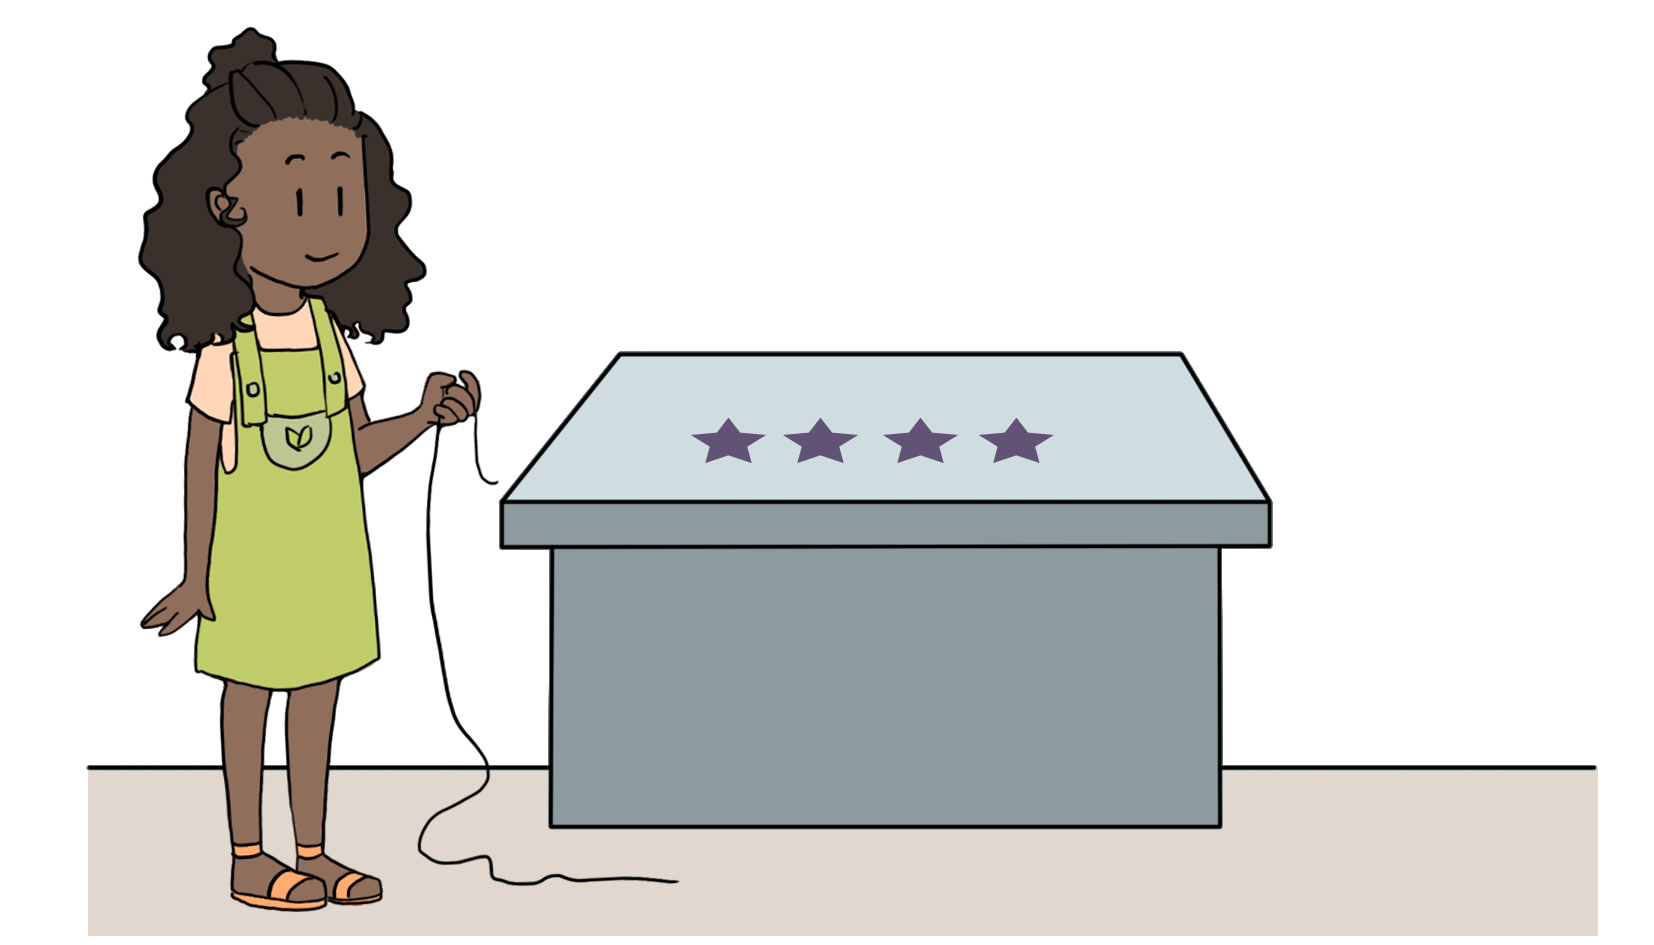
\includegraphics[width=400pt, keepaspectratio]{../figuras/licao01/ativ3_fig01-agnes.png}
  \end{center}

\end{atividade}
\section{ORGANIZANDO AS IDEIAS }

Nas atividades anteriores, a barra de chocolate, a pizza e o pedaço de barbante foram partidos \textbf{em partes com quantidades iguais}.
Em cada um dos casos, o que foi repartido é chamado \textbf{unidade}. Cada uma das partes em que essas unidades foram repartidas igualmente é uma \textbf{fração da unidade}. Assim, por exemplo, um quarto de uma pizza é uma fração da pizza e a pizza é unidade. Se a unidade for um barbante, um quarto do barbante será uma fração do barbante.

\begin{center}
    
\includegraphics[width=300pt, keepaspectratio]{../figuras/licao01/orgideias_fig01-agnes.png}
  \end{center}

O nome dado à fração da unidade depende da quantidade de partes em que a unidade é dividida.
Ao dividir uma unidade qualquer em duas partes iguais, ou ao meio, cada uma das partes é chamada de \textit{um meio} ou \textit{a metade} da unidade.

Por exemplo, se uma barra de chocolate é repartida igualmente entre dois amigos, a quantidade que caberá a cada um dos amigos é \textit{um meio} da barra de chocolate (ou \textit{metade} da barra). Nesse exemplo, a unidade é a barra de chocolate.

\begin{center}
    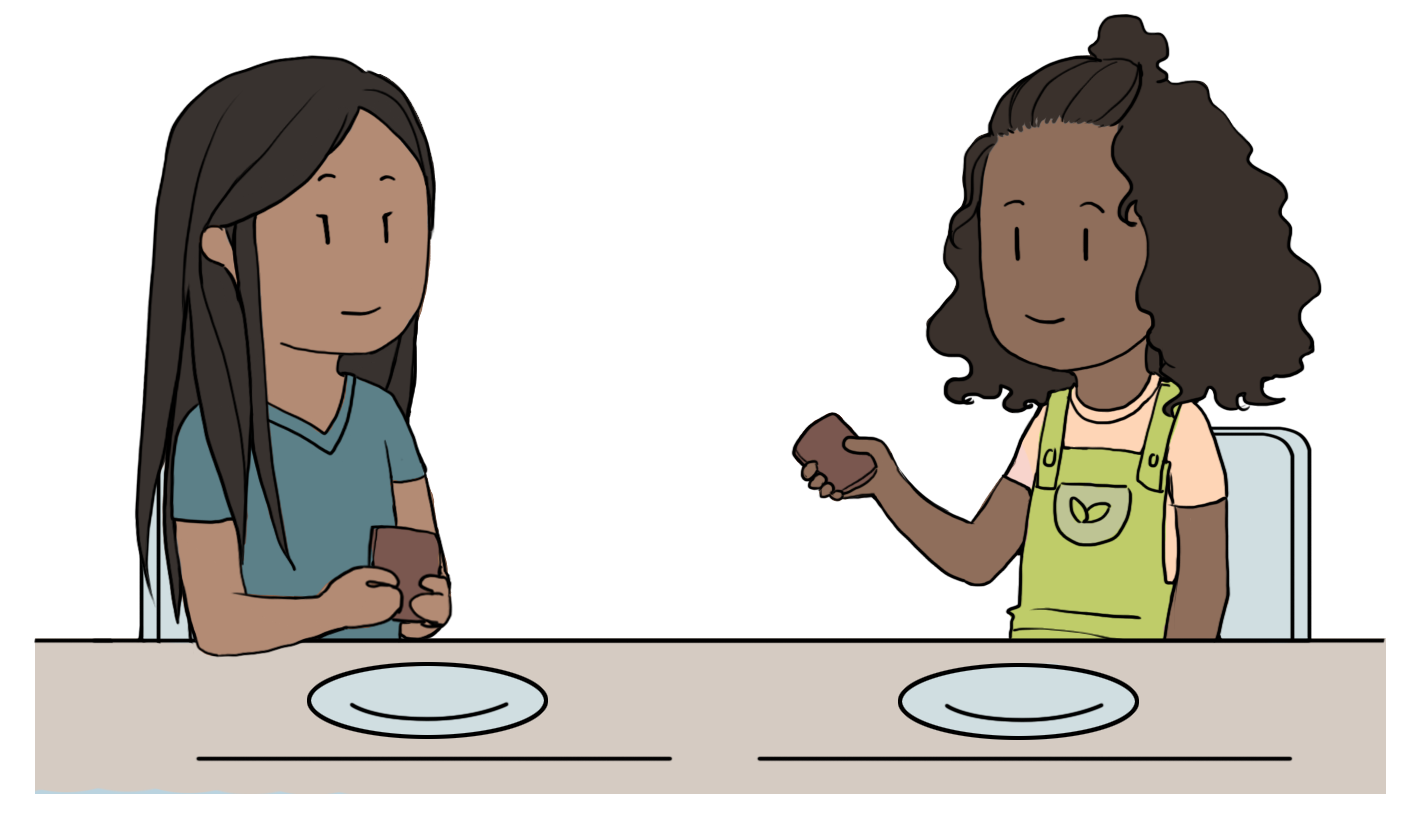
\includegraphics[width=.6\textwidth, keepaspectratio]{../figuras/licao01/orgideias_fig02-agnes.png}
\end{center}

Ao dividir uma unidade em três partes iguais, cada uma das partes é chamada de \textit{um terço} ou \textit{a terça parte} da unidade.

Por exemplo, se, para preparar uma receita, é necessário acrescentar \textit{um terço} de um litro de leite, então para colocar a quantidade correta de leite na receita, é preciso repartir o litro de leite em três partes iguais e usar apenas uma dessas partes. Nesse caso, cada uma das partes é \textit{um terço} do litro de leite. A unidade é um litro de leite.

\begin{center}
    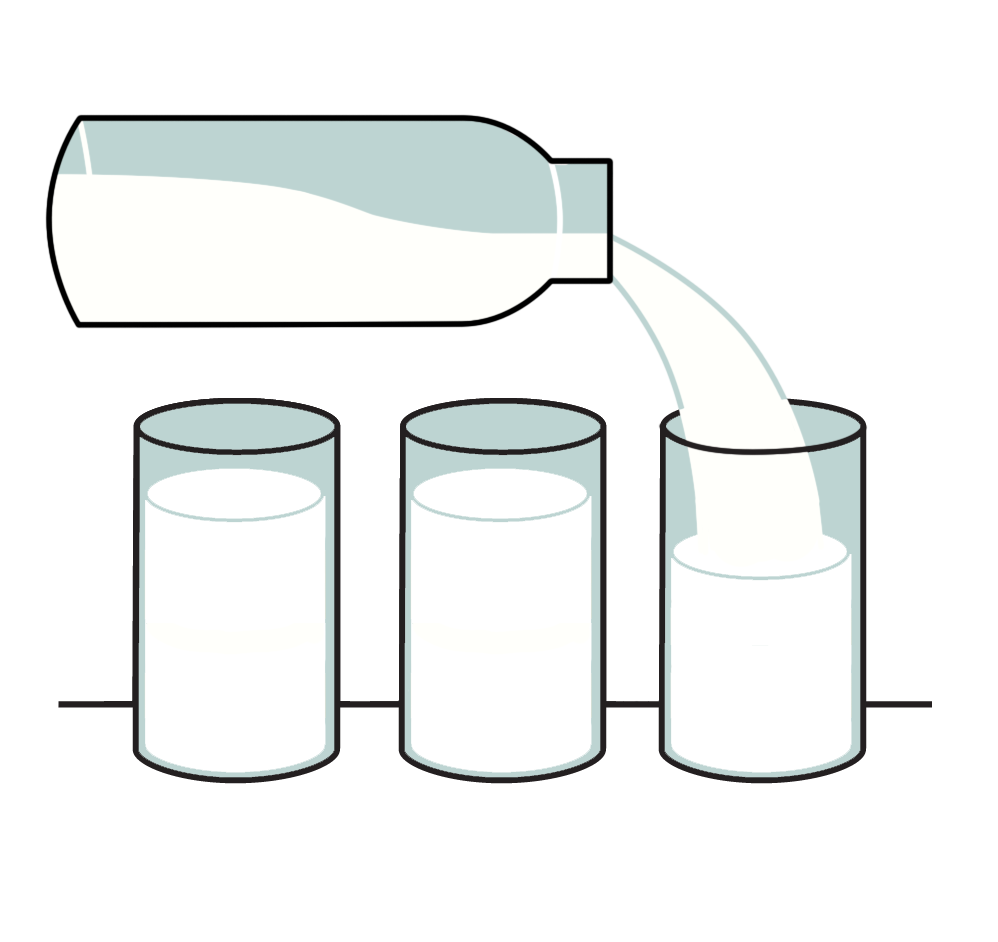
\includegraphics[width=120pt, keepaspectratio]{../figuras/licao01/copos-incompletos-agnes.png} $\quad$ 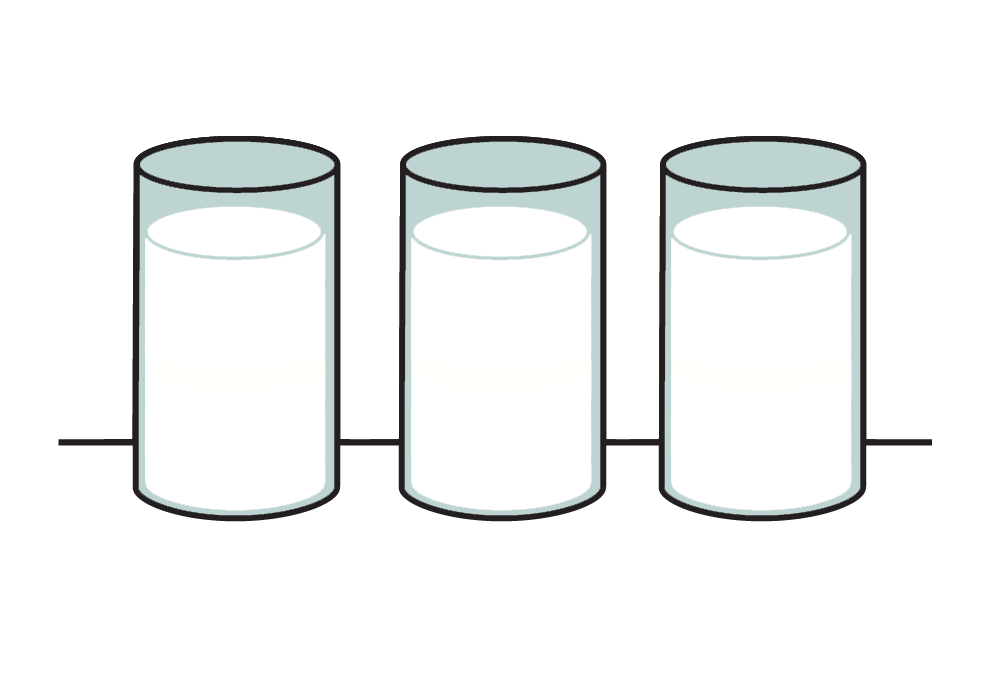
\includegraphics[width=120pt, keepaspectratio]{../figuras/licao01/copos-cheios-agnes.png}
  \end{center}

Ao dividir uma unidade em quatro partes iguais, cada uma das partes é chamada de \textit{um quarto} ou \textit{quarta parte} da unidade.

Por exemplo, a parte colorida da figura é um quarto da figura. Neste caso, a figura é a unidade.

\begin{center}
    
\includegraphics[width=100pt, keepaspectratio]{../figuras/licao01/orgideias_fig04.png}
  \end{center}

Da mesma forma, ao dividir uma unidade em cinco partes iguais, cada uma das partes é chamada de \textit{um quinto} ou \textit{quinta parte} da unidade.

Por exemplo, na época do império \emph{um quinto} de todo ouro pesado nas Casas de Fundição no Brasil era pago em impostos à Coroa Portuguesa. Desta forma, a quantidade de ouro pago em impostos à Coroa Portuguesa era igual a \emph{um quinto} ou a \emph{quinta parte} do ouro pesado nas Casas de Fundição no Brasil.

\begin{center}
    
\includegraphics[width=400pt, keepaspectratio]{../figuras/licao01/orgideias_fig05.png}
  \end{center}

\section{MÃO NA MASSA }

\begin{atividade}{}

\begin{enumerate} [\quad a)] %s
  \item     Quais dos oito retângulos a seguir foram partidos em \textit{quartos}? \newline
 %\vspace{0.2cm}

\begin{center}
 \begin{tikzpicture}[scale=5]
   % primeiro de cima
   % [fill=common, fill opacity=.3]
  \fill[cbpink] (0,0) rectangle (4,6);
  \draw (0,0) rectangle (1,6);
  \draw (1,0) rectangle (2,6);
  \draw (2,0) rectangle (3,6);
  \draw (3,0) rectangle (4,6);
  
  % segundo de cima
  \draw[fill=cbgreen] (5,0) rectangle (9,3);
  \draw[fill=cbgreen] (5,3) rectangle (9,6);
  \draw (5,0) -- (9,3);
  \draw (5,3) -- (9,6);

  \begin{scope}[xshift=28.5]
  % terceiro de cima    
\fill[cbbrown] (0,0) rectangle (4,6);
  \draw(0,0) rectangle (4,1.5);
  \draw (0,1.5) rectangle (4,3);
  \draw (0,3) rectangle (4,4.5);
  \draw (0,4.5) rectangle (4,6);

  % quarto de cima
  \fill[cbolive] (5,0) rectangle (9,6);
  \draw (5,0) rectangle (9,3);
  \draw (5,3) rectangle (9,6);
  \draw (7,0) -- (7,6);

  \end{scope}
  
\end{tikzpicture}

\vspace{0.2cm}

\begin{tikzpicture}[scale=5]

  \begin{scope}[xshift=-28.5]
    % primeiro debaixo
  \fill[cbpurple] (10,0) rectangle (14,6);  
  \draw (10,0) rectangle (14,3);
  \draw (10,3) rectangle (14,6);
  \draw (12,0) -- (12,3);
  \draw (10,4.5) -- (14,4.5);
  
  % 2 debaixo
  %\draw (15,0) rectangle (19,6);
  \filldraw[fill=cbyellow] (15,0) rectangle (19,3);
  \filldraw[fill=cbyellow] (15,3) rectangle (19,6);
  \draw (15,1.5) -- (19,1.5);
 \draw (15,3) -- (19,6);
  \end{scope}
  % 3 debaixo
  \fill[cbgray, opacity=.8] (10,0) rectangle (14,6);
  \draw[fill=cbgray, fill opacity=.3] (10,0) rectangle (14,3);
  \draw[fill=cbgray, fill opacity=.3] (10,3) rectangle (14,6);
  \draw (12,0) -- (12,3);
  \draw (10,6) -- (14,3);

  % 4 debaixo  
  \begin{scope}[xshift=42.5]
  \fill[cborange] (0,0) rectangle (4,6);
  \draw[fill=cborange, fill opacity=.3] (0,0) rectangle (4,6);
  \draw (1,0) -- (1,6);
  \draw (2,0) -- (2,6);
  \draw (2,3) -- (4,3);
  \end{scope}
\end{tikzpicture}
\end{center}

  \item     Desenhe um retângulo e faça uma partição desse retângulo em quatro partes que não sejam todas quartos.
\end{enumerate}
\end{atividade}

\begin{refletindo*}[breakable]{}{}
  Na atividade anterior, as partes em que os retângulos foram divididos são quartos dos retângulos, mesmo tendo formas diferentes.

  \begin{center}
    \begin{tikzpicture}[scale=5]
        \draw[fill=common, fill opacity=.3] (10,0) rectangle (14,3);
  \draw[fill=common, fill opacity=.3] (10,3) rectangle (14,6);
  \draw (12,0) -- (12,3);
  \draw (10,6) -- (14,3);
    \end{tikzpicture}
  \end{center}

  Se uma unidade é repartida em partes com quantidades iguais, essas partes são frações dessa unidade mesmo que tenham formas diferentes. Observe, nos quadrinhos a seguir, como a pizza foi dividida entre os dois amigos:
\begin{center}
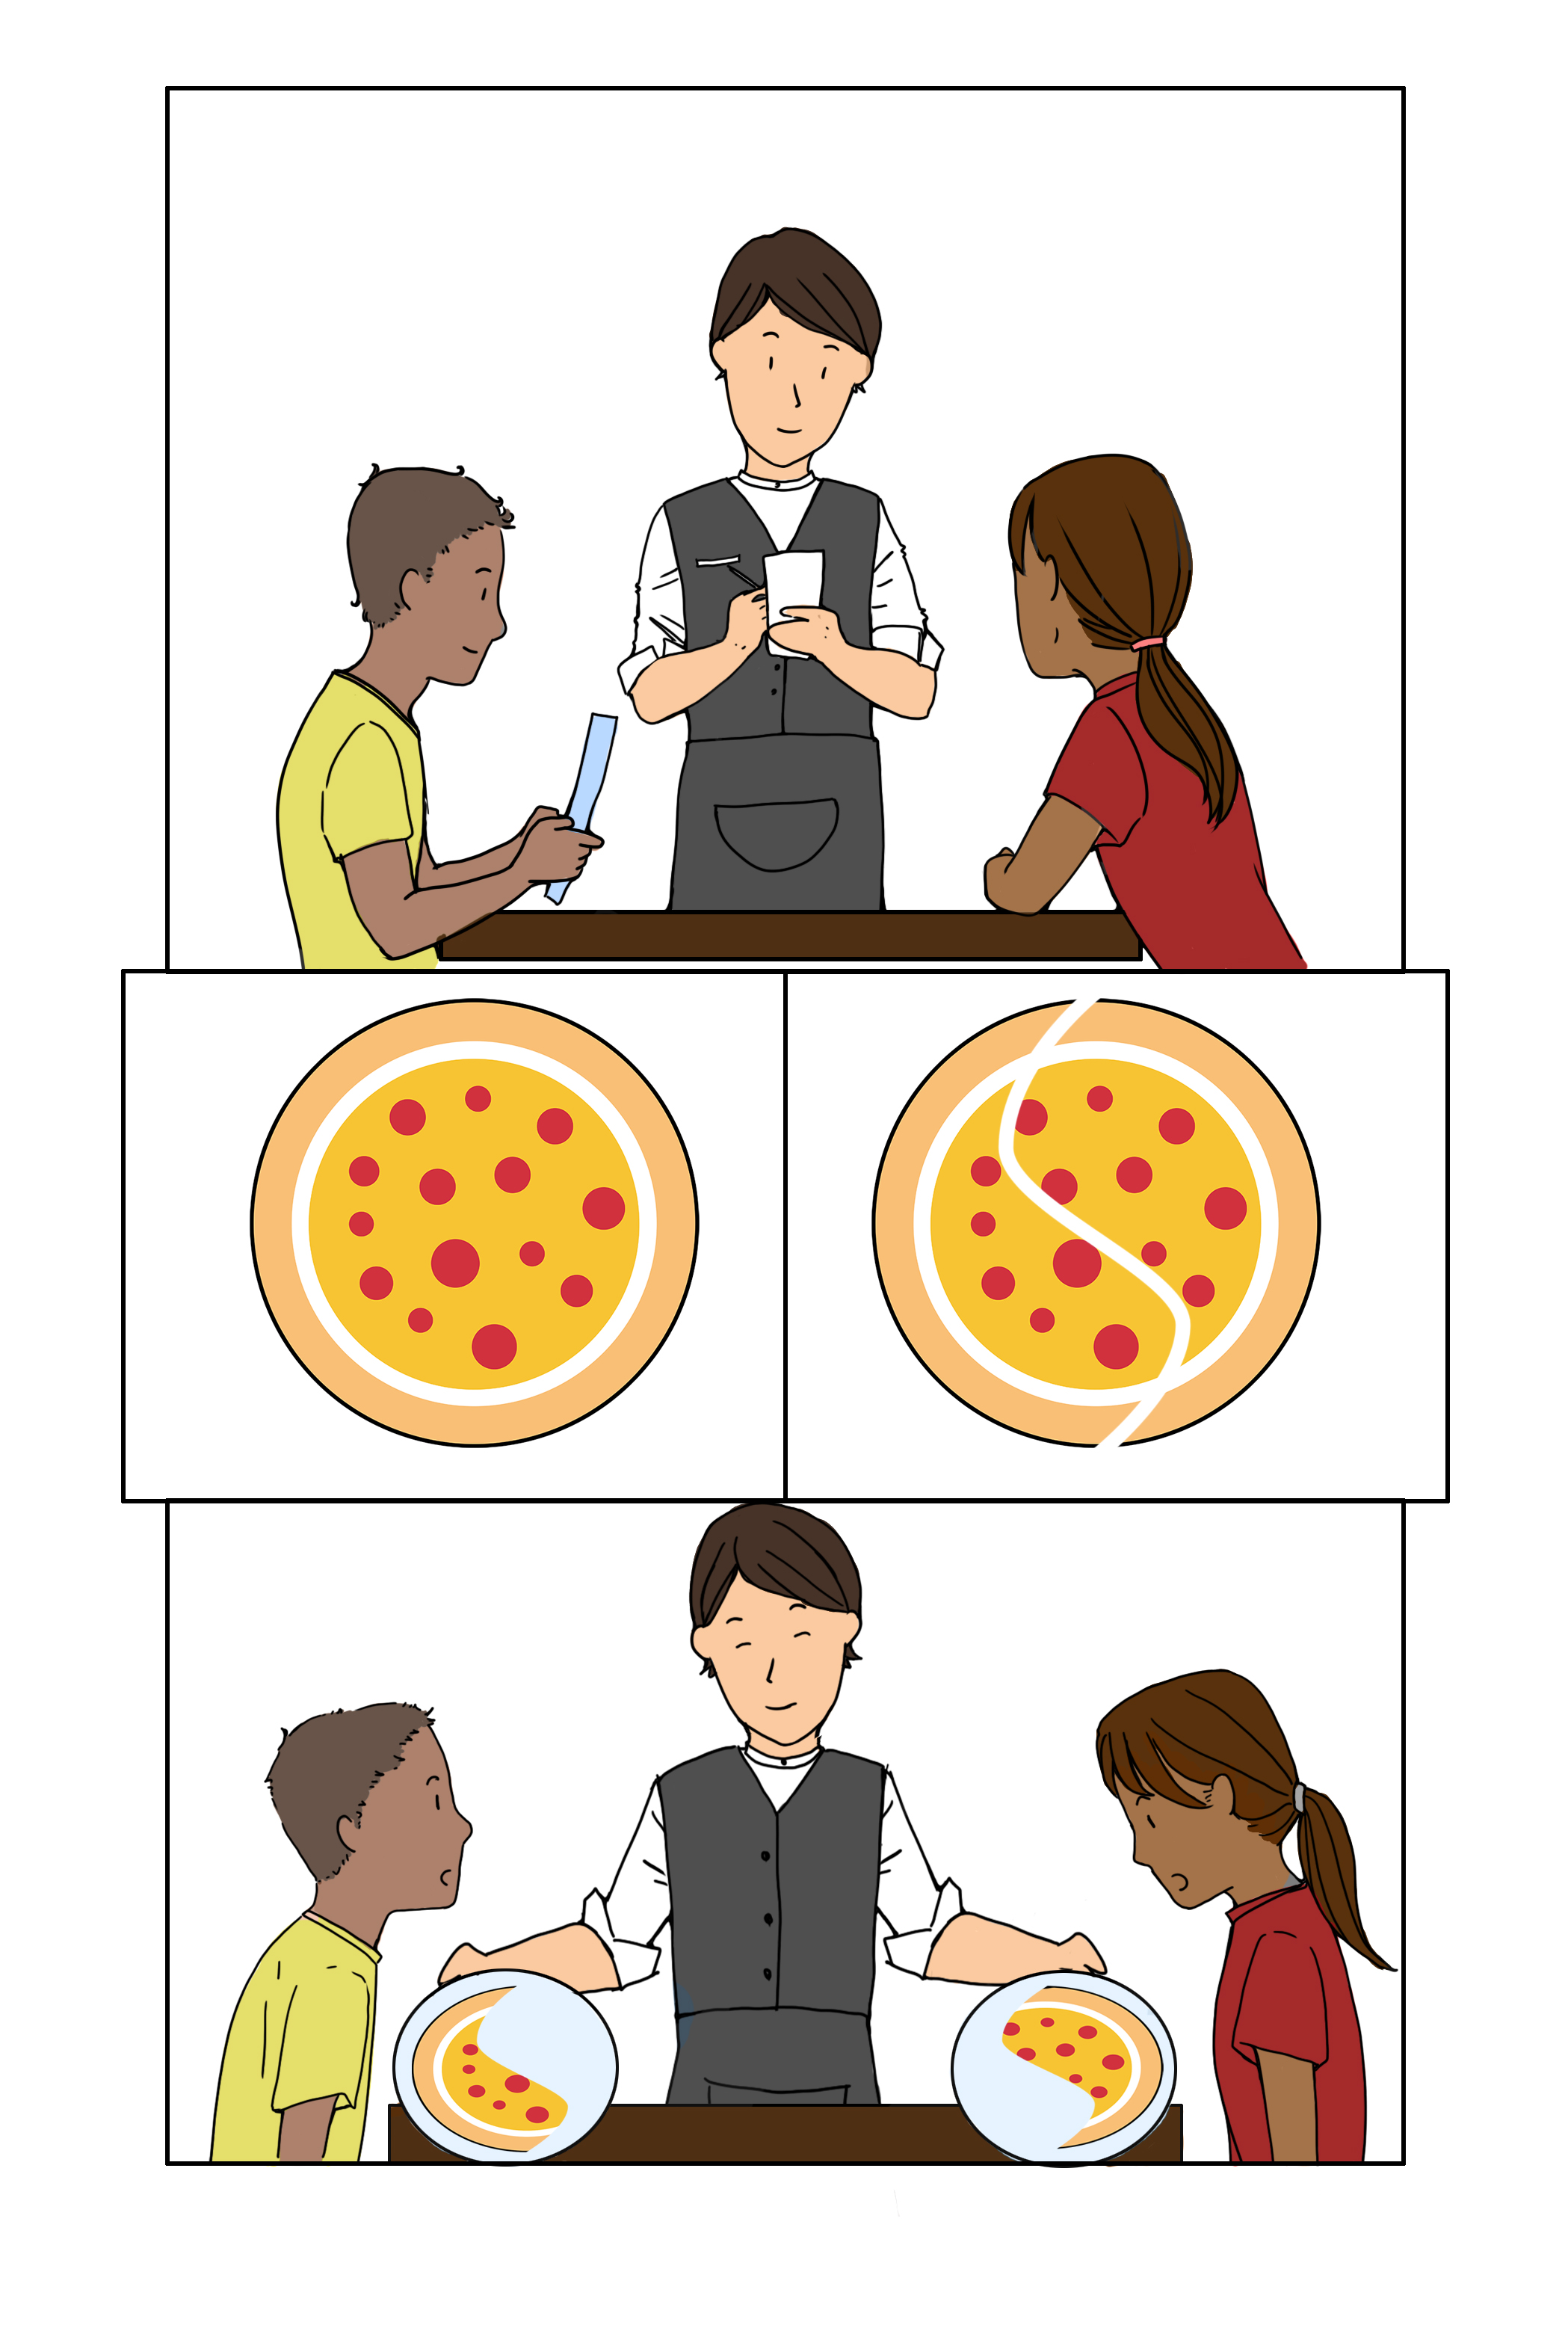
\includegraphics[width=.7\textwidth, keepaspectratio]{../figuras/licao01/pizzaria-do-artista-agnes}
  \end{center}
 % \noindent\begin{tabular}{ll}
  %  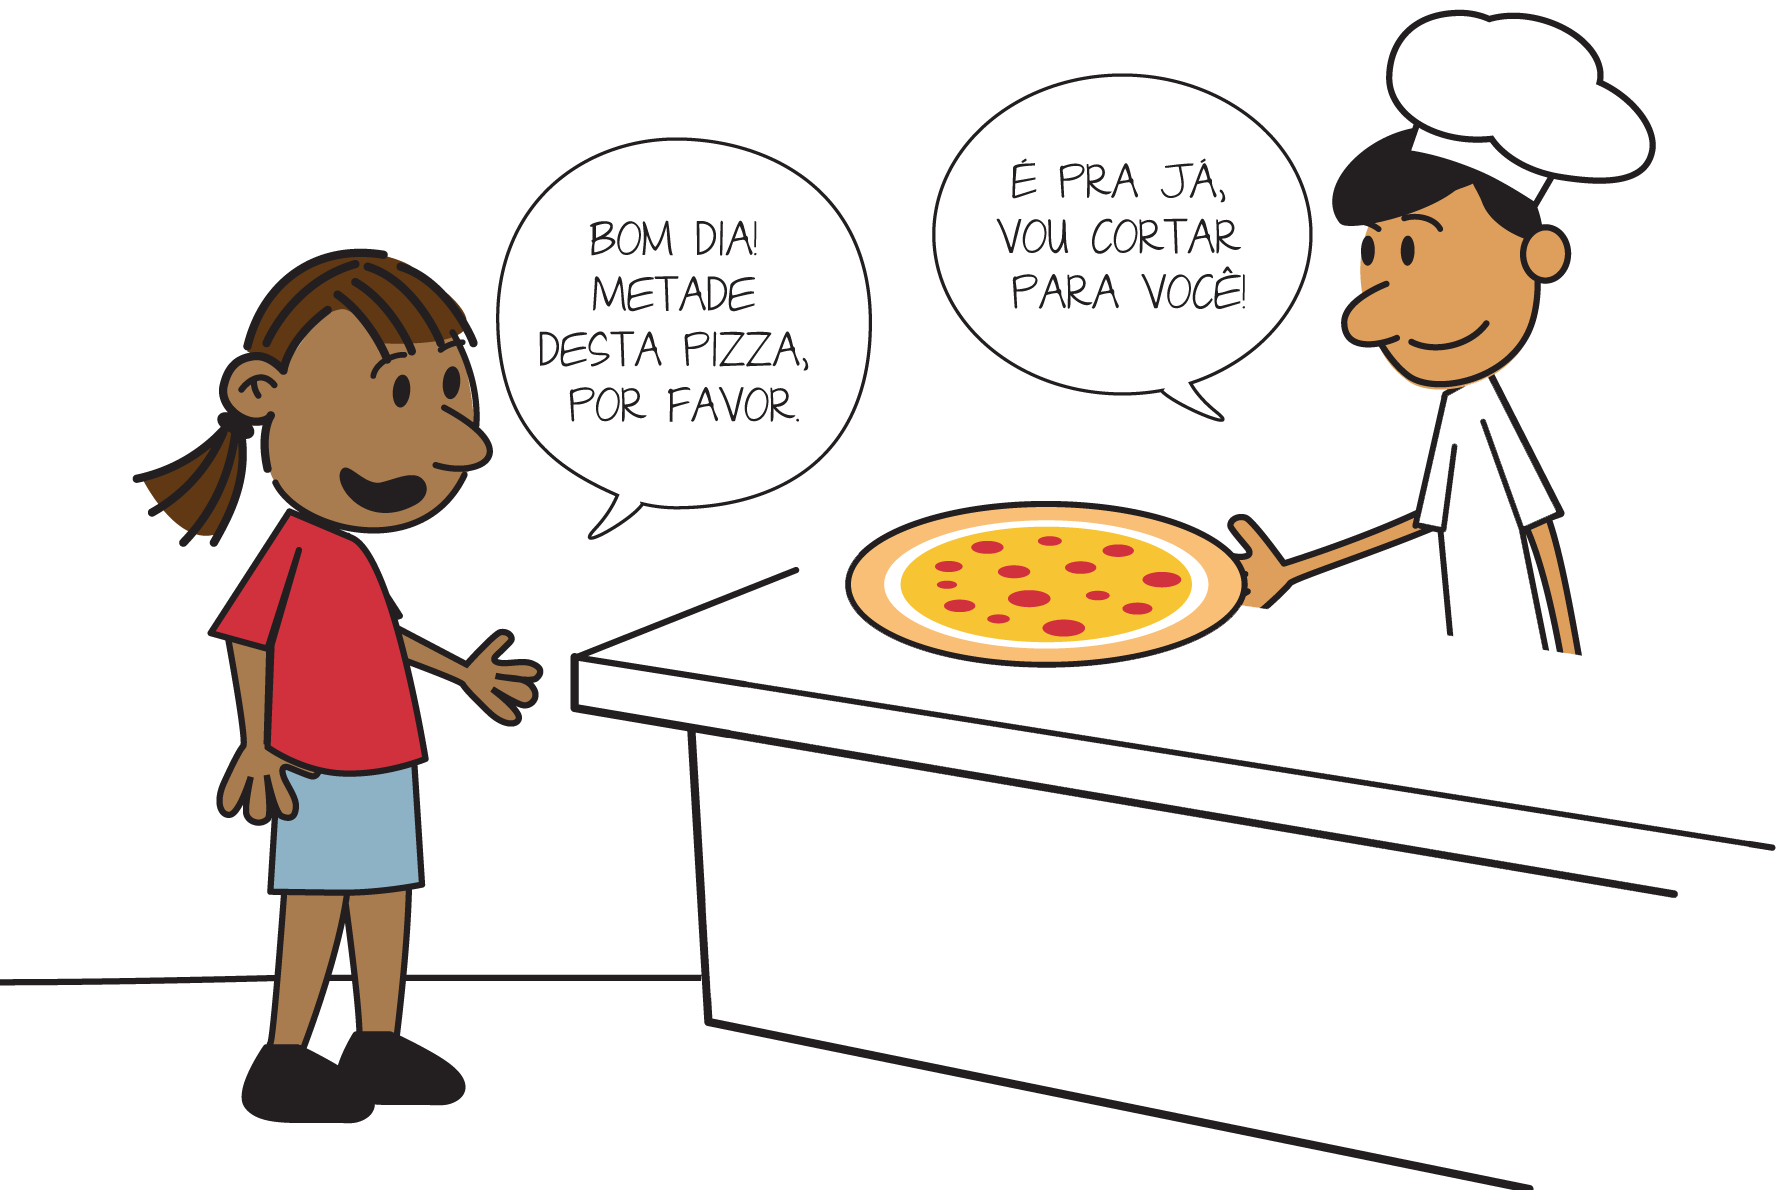
\includegraphics[width=220pt, keepaspectratio]{../figuras/licao01/reflet_fig01.png} & 
\includegraphics[width=180pt, keepaspectratio]{../figuras/licao01/reflet_fig02.png}

  %\end{tabular}
%\vspace{.5cm}
 % \hline
 % \vspace{.5cm}

  %\noindent  \noindent\begin{tabular}{ll}
   % 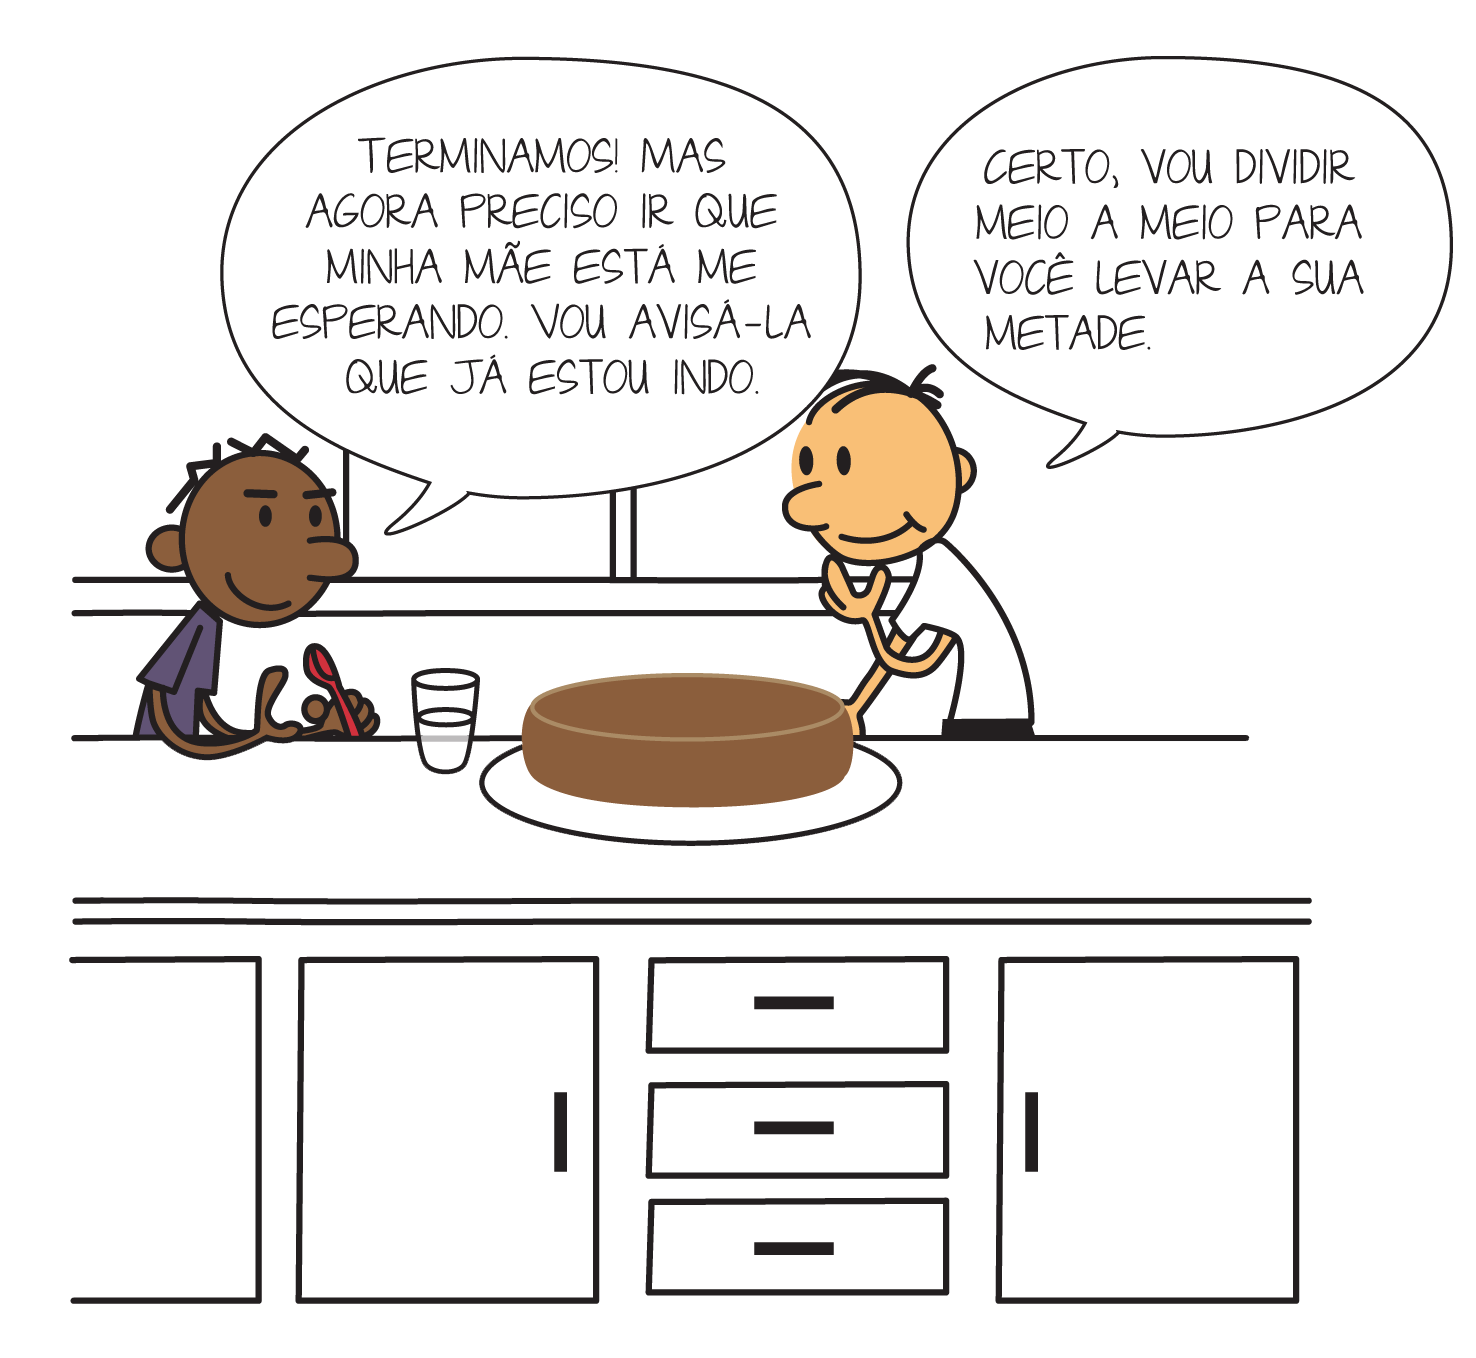
\includegraphics[width=180pt, keepaspectratio]{../figuras/licao01/reflet_fig03.png}   & 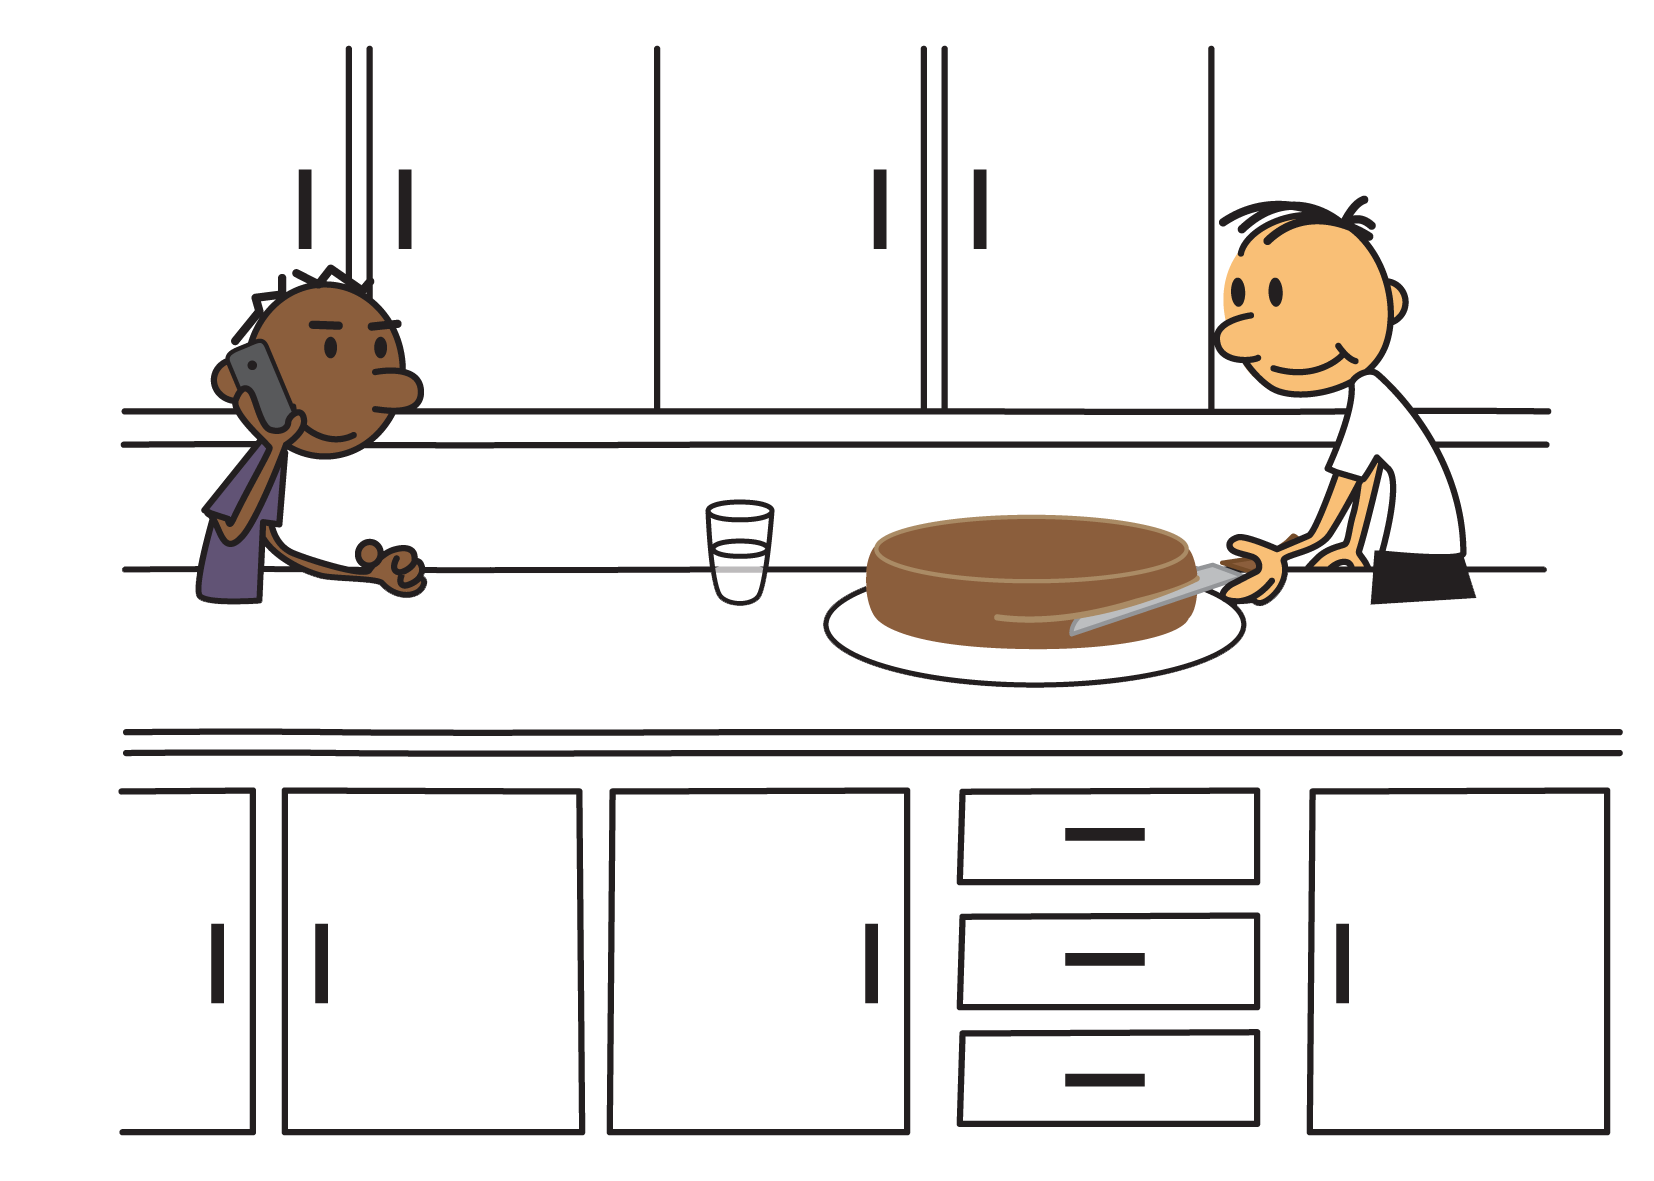
\includegraphics[width=200pt, keepaspectratio]{../figuras/licao01/reflet_fig04.png}
  %\end{tabular}

\end{refletindo*}

\begin{atividade}{}

\begin{enumerate}[a)]
\item O triângulo cinza é um terço de uma das figuras coloridas. Qual é essa figura? Explique. 
\item O triângulo cinza é um quarto de alguma dessas figuras? Qual ou quais?
\item Agora é a sua vez: desenhe uma unidade da qual o triângulo cinza seja um quinto.  
\item Que fração o triângulo cinza é da figura amarela?
\item Desafio: Que fração o triângulo cinza é do retângulo laranja? 
\end{enumerate}

\begin{center}  
\begin{tabular}[c]{ccc}
\begin{tikzpicture}[scale=20]
\fill [cbgray] (60:0) -- (120:1) -- (180:1) -- cycle;
\end{tikzpicture}
  &
%losango
\begin{tikzpicture}[scale=20,rotate=90]
\fill [cbpink] (60:0) -- (120:1) -- (180:1) -- ++(300:1) -- cycle;
\end{tikzpicture}
  &
%estrela de  seis pontas
\begin{tikzpicture}[scale=20]
\fill [cbpurple] (0,0) -- (60:1) -- (120:1) -- cycle;
\fill [cbpurple,shift={(.5,1.71/6)}] (60:0) -- (120:1) -- (180:1) -- cycle;
\end{tikzpicture}
    \\
%paralelogramo
\begin{tikzpicture}[scale=20]
\fill [cbgreen]  (120:1) -- ++(180:1) -- ++(240:1) -- ++(360:2) -- ++(60:1) -- cycle;
\end{tikzpicture}
  &
%retângulo
\begin{tikzpicture}[scale=20]
\fill [cborange] (0,0) -- (1,0) -- (1,1.732/2) -- (0,1.732/2) -- cycle;
\end{tikzpicture}
  &
    %trapézio:
\begin{tikzpicture}[scale=20]
\fill [cbpink] (60:0) -- (120:1) -- ++(180:1) -- +(240:1) -- cycle;
\end{tikzpicture}
  \\
  %hexágono
\begin{tikzpicture}[scale=20]
\fill [cbolive] (60:0) -- (120:1) -- ++(180:1) -- ++(240:1) -- ++(300:1) -- ++(360:1) -- cycle;
\end{tikzpicture}
&
%Bandeirinha
\begin{tikzpicture}[scale=20,xscale=-1]
\filldraw [cbyellow]  (120:1) -- ++(180:1) -- ++(240:1) -- ++(360:2) -- ++(60:1) -- cycle;
\fill [cbyellow,yscale=-1]  (120:1) -- ++(180:1) -- ++(240:1) -- ++(360:2) -- ++(60:1) -- cycle;
\end{tikzpicture}
&
%Triângulo ampliado
\begin{tikzpicture}[scale=40]
\fill [cbbrown] (60:0) -- (120:1) -- (180:1) -- cycle;
\end{tikzpicture}
\end{tabular}
\end{center}

\end{atividade}
\begin{atividade}{}

Em cinco das figuras a seguir, a parte em vermelho é um terço da figura. Identifique essas figuras.

\begin{center}
\begin{longtable}{ccc}
a)
\parbox[t][3cm][c]{5cm}{
  \begin{tikzpicture}[scale=0.7]
    \draw[very thick, attention] (90:2 cm)  -- (210:2 cm);
    \draw[very thick, attention] (330:2 cm) -- (90:2 cm);
    \draw[very thick, common] (210:2 cm)  -- (330:2 cm);
  \end{tikzpicture}
}
& \quad \quad  &


b)
\parbox[t][3cm][c]{5cm}{
\begin{tikzpicture}[scale=0.7]
  \draw[very thick, common] (90:2 cm)  -- (210:2 cm);
  \draw[very thick, attention] (210:2 cm)  -- (330:2 cm);
  \draw[very thick, common] (330:2 cm) -- (90:2 cm);
\end{tikzpicture}
}
\\


c)
\parbox[t][3cm][c]{5cm}{
\begin{tikzpicture}[scale=4]
  \draw[very thick, common] (0,3) -- (3,0);
  \draw[very thick, attention] (3,0) -- (6,3);
  \draw[very thick, common] (6,3) -- (9,0);
\end{tikzpicture}
}
& &


d)
\parbox[t][3cm][c]{5cm}{
  \begin{tikzpicture}[scale=4]
    \draw[very thick, attention] (0,3) -- (3,0);
    \draw[very thick, attention] (3,0) -- (6,3);
    \draw[very thick, common] (6,3) -- (9,0);
  \end{tikzpicture}
}

\\
e)
\parbox[t][3cm][c]{5cm}{
\begin{tikzpicture}[scale=3]
    \draw[fill=common, fill opacity=.3] (0,0) rectangle (3,1);
    \draw[fill=attention] (3,0) rectangle (6,1);
    \draw[fill=common, fill opacity=.3] (6,0) rectangle (9,1);
\end{tikzpicture}
}
& &

f)
\parbox[t][3cm][c]{5cm}{
\begin{tikzpicture}[scale=3]
    \draw[fill=common, fill opacity=.3] (0,0) rectangle (2,1);
    \draw[fill=attention] (2,0) rectangle (6,1);
    \draw[fill=common, fill opacity=.3] (6,0) rectangle (9,1);
\end{tikzpicture}
}
\\
g)
\parbox[t][3cm][c]{5cm}{
\begin{tikzpicture}[scale=0.7]

\filldraw [fill=common, fill opacity=.3, draw=black] (0:2 cm) -- (90:2 cm) -- (180:2 cm) -- (0,0) -- ( (270:2 cm) --cycle;
\fill[attention] (180:2 cm) -- (270:2cm) -- (0,0) -- cycle;
\draw (180:2 cm) -- (0:2 cm);
\draw (90:2 cm) -- (270:2 cm);
\draw (180:2 cm) -- (270:2 cm);
\end{tikzpicture}
}
&&
h)
\parbox[t][3cm][c]{5cm}{
\begin{tikzpicture}[scale=0.7]
  \filldraw[fill=attention, draw=black] (-2 cm, 0) -- (0,0) -- (0, 2 cm) arc (90:180:2 cm) -- cycle;
  \filldraw[fill=common, draw=black, fill opacity=.3] (-2 cm, 0) -- (2 cm,0) arc (0:-180: 2cm);
  \fill (0,0) circle (2 pt);
\end{tikzpicture}
}
\\
i)
\parbox[t][3cm][c]{5cm}{
\begin{tikzpicture}[scale=6]
  \filldraw[fill=common, fill opacity=.3, draw=black] (0,0) -- (0.5,0.5) -- (4,0.5) -- (4,2) -- (4.5,2.5) -- (4.5,0)--cycle;
  \fill[attention] (0,0) -- (0.5,0.5) -- (0.5,2) -- (4,2) -- (4.5,2.5) -- (0,2.5)--cycle;
 \draw (0,0) rectangle (4.5,2.5);
  \draw (0.5,0.5) rectangle (4,2);
\end{tikzpicture}
}
& &


j)
\parbox[t][3cm][c]{5cm}{

%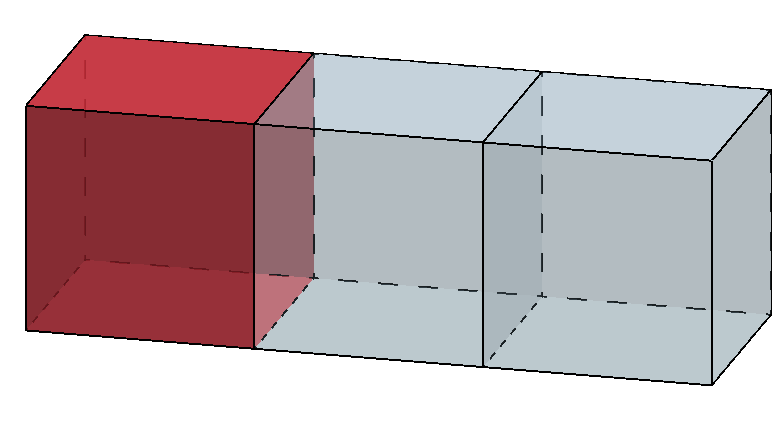
\includegraphics[scale=.6]{..figuras/licao01/paralelepipedo_tercos.png}
%}
  \begin{tikzpicture}%[scale=60]
  \tikzset{
  annotated cuboid/.pic={
    \tikzset{%
      every edge quotes/.append style={midway, auto},
      /cuboid/.cd,
      #1
    }
    \draw [every edge/.append style={pic actions, densely dashed, opacity=0}, pic actions]
    (0,0,0) coordinate (o) -- ++(-\cubescale*\cubex,0,0) coordinate (a) -- ++(0,-\cubescale*\cubey,0) coordinate (b) edge coordinate [pos=1] (g) ++(0,0,-\cubescale*\cubez)  -- ++(\cubescale*\cubex,0,0) coordinate (c) -- cycle
    (o) -- ++(0,0,-\cubescale*\cubez) coordinate (d) -- ++(0,-\cubescale*\cubey,0) coordinate (e) edge (g) -- (c) -- cycle
    (o) -- (a) -- ++(0,0,-\cubescale*\cubez) coordinate (f) edge (g) -- (d) -- cycle;
 },
  /cuboid/.search also={/tikz},
  /cuboid/.cd,
  width/.store in=\cubex,
  height/.store in=\cubey,
  depth/.store in=\cubez,
  units/.store in=\cubeunits,
  scale/.store in=\cubescale,
  width=100,
  height=100,
  depth=100,
  units=cm,
  scale=.1,
}

    \pic [fill=attention] at (50,0) {annotated cuboid={width=100, height=100, depth=14}};
    \pic [fill=common, fill opacity=.3] at (70,0) {annotated cuboid={width=200, height=100, depth=14}};
    \draw [dashed, lightgray] (50,-10,-1.4) -- (70,-10,-1.4);
    \draw [dashed, lightgray] (60,-10,0) -- (60,-10,-1.4) -- (60,0,-1.4);
    \draw [dashed] (60,0,-1.4) -- (60,0,0) -- (60,-10,0);
    \end{tikzpicture}
}


\end{longtable}
\end{center}

\end{atividade}

\begin{atividade}{}


\begin{enumerate}[a)]
\item Na tabela a seguir, a primeira coluna mostra uma figura que é uma fração de uma unidade. Na segunda, o nome que usamos para essa fração. Desenhe uma unidade na terceira coluna, unindo frações como essa.
  
  \def\h{1.8}
  
\begin{center}
  \begin{tabular}{|m{0.3\linewidth}|m{0.3\linewidth}|m{0.3\linewidth}|}
  \hline
\centering Fração da unidade & \centering Nome da fração da unidade  & \quad\quad\quad Unidade  \\
\hline \hline
\centering \begin{tikzpicture}[scale=2]
 \draw [fill=common, fill opacity=.3] (0,0) arc (0:90:3) -- (-3,0) -- cycle;
\end{tikzpicture}
&\centering \parbox[c][\h cm][c]{0.01cm}{  } metade  &  \\
    \hline
  \end{tabular}
\end{center}

\item A seguir, complete cada linha da tabela como no item anterior.
  
\begin{center}
  \begin{longtable}{|m{0.3\linewidth}|m{0.3\linewidth}|m{0.3\linewidth}|}
  \hline
\centering Fração da unidade & \centering Nome da fração da unidade  & \quad\quad\quad Unidade  \\
\hline \hline
\endhead
\centering \begin{tikzpicture}[scale=2]
 \draw [fill=common, fill opacity=.3] (0,0) arc (0:90:3) -- (-3,0) -- cycle;
\end{tikzpicture}
&\centering \parbox[c][\h cm][c]{0.01cm}{  } metade  &  \\
    \hline
\centering\begin{tikzpicture}[scale=2]
\draw [fill=common, fill opacity=.3] (0,0) arc (0:90:3) -- (-3,0) -- cycle;
\end{tikzpicture}        &\parbox[c][\h cm][c]{0.01cm}{  } \centering   um terço  &  \\
    \hline
\centering \begin{tikzpicture}[scale=2]
\draw [fill=common, fill opacity=.3] (0,0) arc (0:90:3) -- (-3,0) -- cycle;
\end{tikzpicture}        & \centering \parbox[c][\h cm][c]{0.01cm}{  } um quarto  &  \\
    \hline
\centering \begin{tikzpicture}[scale=2]
\draw [fill=common, fill opacity=.3] (0,0) rectangle (3,3);
\end{tikzpicture}
  & \centering \parbox[c][\h cm][c]{0.01cm}{  } metade  &  \\
    \hline
\centering \begin{tikzpicture}[scale=2]
\draw [fill=common, fill opacity=.3] (0,0) rectangle (3,3);
\end{tikzpicture}
  & \centering \parbox[c][\h cm][c]{0.01cm}{  } um terço  &  \\
    \hline
\centering \begin{tikzpicture}[scale=2]
\draw [fill=common, fill opacity=.3] (0,0) rectangle (3,3);
\end{tikzpicture}
 & \centering \parbox[c][\h cm][c]{0.01cm}{  } um quarto  &  \\
    \hline
\centering \begin{tikzpicture}[scale=2]
\draw  (0,0) -- (3,3);
\end{tikzpicture}
  & \centering \parbox[c][\h cm][c]{0.01cm}{  } metade  &  \\
    \hline
\centering \begin{tikzpicture}[scale=2]
\draw  (0,0) -- (3,3);
\end{tikzpicture}
  & \centering \parbox[c][\h cm][c]{0.01cm}{  } um terço  &  \\
    \hline
\centering \begin{tikzpicture}[scale=2]
\draw  (0,0) -- (3,3);
\end{tikzpicture}
  & \centering \parbox[c][\h cm][c]{0.01cm}{  } um quarto  &  \\
    \hline
\centering \begin{tikzpicture}[scale=2]
\draw [fill=common, fill opacity=.3] (90:2) -- (210:2) -- (330:2) -- cycle;
\end{tikzpicture}  & \centering \parbox[c][\h cm][c]{0.01cm}{  } metade  &  \\
    \hline
\centering \begin{tikzpicture}[scale=2]
\draw [fill=common, fill opacity=.3] (90:2) -- (210:2) -- (330:2) -- cycle;
\end{tikzpicture}  & \centering \parbox[c][\h cm][c]{0.01cm}{  } um terço  &  \\
    \hline
\centering \begin{tikzpicture}[scale=2]
\draw [fill=common, fill opacity=.3] (90:2) -- (210:2) -- (330:2) -- cycle;
\end{tikzpicture}  & \centering \parbox[c][\h cm][c]{0.01cm}{  } um quarto  &  \\
    \hline
  \end{longtable}
\end{center}

\end{enumerate}
% \pagebreak
\end{atividade}
\begin{atividade}{}

\begin{enumerate} [\quad a)] %s
  \item     Pinte metade do quadrado a seguir.

  \begin{center}
 \begin{tikzpicture}[x=1mm,y=1mm, scale=.7]  \draw[fill=common, fill opacity=.3] (0,0) rectangle (20,20);  \end{tikzpicture}
  \end{center}

  \item     Pinte um quarto do quadrado a seguir.

  \begin{center}
 \begin{tikzpicture}[x=1mm,y=1mm, scale=.7]  \draw[fill=common, fill opacity=.3] (0,0) rectangle (20,20);  \end{tikzpicture}
  \end{center}

  \item     Pinte um oitavo do quadrado a seguir.

  \begin{center}
 \begin{tikzpicture}[x=1mm,y=1mm, scale=.7]  \draw[fill=common, fill opacity=.3] (0,0) rectangle (20,20);  \end{tikzpicture}
  \end{center}
  \item     Qual é a maior das frações do quadrado: metade, quarto ou oitavo?
\end{enumerate} %s
\end{atividade}

\begin{atividade}{}

\begin{enumerate} [a)] %d
  \item     Pinte metade da figura.
\begin{center}
  \begin{tikzpicture}[x=1cm,y=1cm, scale=0.5]
  \draw[fill=common, fill opacity=.3] (3.,5.) -- (3.,3.) -- (4.7,2.) -- (6.46,3.) -- (8.2,2.) -- (9.9,3.) -- (9.9,5.) -- (8.2,6.)       -- (6.46,5.) -- (4.73,6.) -- cycle;
  \end{tikzpicture}
\end{center}

  \item     Pinte metade da figura de forma diferente da do item anterior.
\begin{center}
  \begin{tikzpicture}[x=1cm,y=1cm, scale=0.5]
  \draw[fill=common, fill opacity=.3] (3.,5.) -- (3.,3.) -- (4.7,2.) -- (6.46,3.) -- (8.2,2.) -- (9.9,3.) -- (9.9,5.) -- (8.2,6.)       -- (6.46,5.) -- (4.73,6.) -- cycle;
  \end{tikzpicture}
\end{center}

  \item     Pinte a metade da figura de forma diferente das dos dois itens anteriores.
\begin{center}
  \begin{tikzpicture}[x=1cm,y=1cm, scale=0.5]
  \draw[fill=common, fill opacity=.3] (3.,5.) -- (3.,3.) -- (4.7,2.) -- (6.46,3.) -- (8.2,2.) -- (9.9,3.) -- (9.9,5.) -- (8.2,6.)       -- (6.46,5.) -- (4.73,6.) -- cycle;
  \end{tikzpicture}
\end{center}


\end{enumerate} %d
\end{atividade}

\begin{atividade}[label=chap1-ativ10]{}
\phantomsection

Identifique as figuras em que a parte pintada de vermelho é a metade da figura.

\begin{center}
  \begin{tabular}{ccccc}
%retângulos

\begin{tikzpicture}[scale=5]
 \draw[fill=attention] (0,0) rectangle (3,2);
 \draw[fill=common, fill opacity=.3] (3,0) rectangle (6,2);
 \node at (3,-1) {Figura 1};
\end{tikzpicture}
&
\quad \quad \quad
&
\begin{tikzpicture}[scale=5]
 \draw[fill=common, fill opacity=.3] (0,0) rectangle (3,2);
 \draw (1,0) -- (1,2);
 \draw (1.5,0) -- (1.5,2);
 \draw (2.2,0) -- (2.2,2);
 \draw[fill=attention] (3,0) rectangle (6,2);
 \node at (3,-1) {Figura 2};
\end{tikzpicture}
&
\quad \quad \quad
&

\begin{tikzpicture}[scale=5]
 \draw[fill=common, fill opacity=.3] (0,0) rectangle (3,2);
 \draw[fill=common, fill opacity=.3] (3,0) rectangle (6,2);
 \node at (3,-1) {Figura 3};
 \filldraw[fill=attention, draw=black] (0,2) rectangle (6,1.2);
 \end{tikzpicture}
\\
 % círculos

\begin{tikzpicture}[scale=5]
  \filldraw[fill=attention, draw=black] (0,-2) arc (-90:90: 2);
  \draw (0, 2) -- (0, -2);
  \draw[fill=common, fill opacity=.3] (0,2) arc (90:270:2);
  \node at (0,-3) {Figura 4};
\end{tikzpicture}
&&

\begin{tikzpicture}[scale=5]
 \filldraw[fill=attention, draw=black] (45:2) arc (45:225:2);
 \draw[fill=common, fill opacity=.3] (225:2) arc (225:405:2);
 \node at (0,-3) {Figura 5};
 \draw (0,0) -- (0,-2);
 \draw (0,0) -- (-30:2);
 \draw (225:2) -- (45:2);
 \end{tikzpicture}

 &&
 \begin{tikzpicture}[scale=5]
 \draw[fill=common, fill opacity=.3] (0,0) circle (2);
 \filldraw[fill=attention, draw=black] (0,0) -- (2,0) arc (0:90:2) -- cycle;
 \filldraw[fill=attention, draw=black] (0,0) -- (-2,0) arc (180:270: 2) -- cycle;
 \node at (0,-3) {Figura 6};
\end{tikzpicture}
\\
% hexágonos

\begin{tikzpicture}[scale=5]
 \filldraw[fill=common, fill opacity=.3] (60:2) -- (120:2) -- (180:2) -- (240:2) -- (300:2) --cycle;
 \filldraw[fill=attention, draw=black] (2,0) -- (60:2) -- (300:2) --cycle;
 \node at (0,-3) {Figura 7};
\end{tikzpicture}
& &

\begin{tikzpicture}[scale=5]
  \filldraw[fill=attention, draw=black] (60:2) -- (120:2) -- (180:2) -- (240:2) --cycle;
\filldraw[fill=common, fill opacity=.3] (60:2) -- (240:2) -- (300:2) -- (0:2) --cycle;
  \draw (60:2) -- (0,0) -- (240:2);
  \draw (2,0) -- (0,0) -- (300:2) (0,-3) node{Figura 8};
\end{tikzpicture}
&&

\begin{tikzpicture}[scale=5]
  \filldraw[fill=attention] (0:2) -- (60:2) -- (0:0) --cycle;
  \filldraw[fill=attention] (120:2) -- (180:2) -- (0:0) --cycle;
  \filldraw[fill=attention] (240:2) -- (300:2) -- (0:0) --cycle;
  \filldraw[fill=common, fill opacity=.3] (0,0) -- (60:2) -- (120:2)--cycle;
  \filldraw[fill=common, fill opacity=.3] (0,0) -- (0:2) -- (300:2)--cycle;
  \filldraw[fill=common, fill opacity=.3] (0,0) -- (180:2) -- (240:2)--cycle;
  \node at (0,-3) {Figura 9};
\end{tikzpicture}
\\
%círculo

\begin{tikzpicture}[scale=5]
 \draw[fill=attention] (0:2) arc (0:270:2) -- (0,0) -- cycle;
 \draw[fill=common, fill opacity=.3] (270:2) arc (270:360:2) -- (0,0) -- cycle;
 \draw (0,0) -- (0,-2);
 \draw (0,0) -- (2,0)  (0,-3) node{Figura 10};
 \end{tikzpicture}
&&
%hexágonos

\begin{tikzpicture}[scale=5]
  \filldraw[fill=attention] (120:2) -- (180:2) -- (240:2) -- cycle;
  \filldraw[fill=attention] (240:2) -- (300:2) -- (60:2) -- cycle;
  \draw[fill=common, fill opacity=.3] (60:2) -- (120:2) -- (240:2) -- cycle;
  \draw[fill=common, fill opacity=.3] (0:2) -- (300:2) -- (60:2) -- cycle;
  \node at (0,-3) {Figura 11};
\end{tikzpicture}
&&
%retângulo
\begin{tikzpicture}[scale=5]
 \draw[fill=common, fill opacity=.3] (0,-1) rectangle (6,1);
 \filldraw[fill=attention, draw=black] (1,-1) rectangle (4,1);
 \node at (3,-2) {Figura 12};
 \end{tikzpicture}

\end{tabular}
\end{center}
\end{atividade}

\begin{atividade}{}

Você receberá do seu professor círculos como os que seguem, todos de mesmo tamanho. 

\begin{center}

 \begin{tabular}{ccccccccc}

 \begin{tikzpicture}
\fill[black] (0,0) circle (10);
 \end{tikzpicture}
& \parbox[t][.6cm][c]{1cm}{ }\quad&
 \begin{tikzpicture}
\fill[pink] (0,0) circle (10);
\draw[line width =.25mm, white] (-90:10) -- (90:10);
\end{tikzpicture}
& \quad&
 \begin{tikzpicture}
\fill[common] (0,0) circle (10);
\foreach \x in {30,150,270} \draw[line width =.25mm, white] (0,0)--(\x:10);
\end{tikzpicture}
& \quad&
 \begin{tikzpicture}
\fill[attention] (0,0) circle (10);
\foreach \x in {0,90} \draw[line width =.25mm, white] (\x:-10)--(\x:10);
\end{tikzpicture}
& \quad&
 \begin{tikzpicture}
\fill[OliveGreen] (0,0) circle (10);
\foreach \x in {18,90,...,360} \draw[line width =.25mm, white] (0,0)--(\x:10);
\end{tikzpicture}\\
\begin{tikzpicture}
\fill[Purple] (0,0) circle (10);
\foreach \x in {0,60,...,360} \draw[line width =.25mm, white] (0,0)--(\x:10);
\end{tikzpicture}
& \parbox[t][.6cm][c]{1cm}{ }\quad&
\begin{tikzpicture}
\fill[yellow] (0,0) circle (10);
\foreach \x in {0,51.428,...,360} \draw[line width =.25mm, white] (0,0)--(\x:10);
\end{tikzpicture}
&\parbox[t][.6cm][c]{1cm}{ }&
\begin{tikzpicture}
\fill[gray] (0,0) circle (10);
\foreach \x in {0,45,...,360} \draw[line width =.25mm, white] (0,0)--(\x:10);
\end{tikzpicture}
& \quad&
\begin{tikzpicture}
\fill[orange] (0,0) circle (10);
\foreach \x in {0,40,...,360} \draw[line width =.25mm, white] (0,0)--(\x:10);
\end{tikzpicture}
& \quad&
\begin{tikzpicture}
\draw (0,0) circle (10);
\foreach \x in {0,36,...,360} \draw[line width =.25mm] (0,0)--(\x:10);
\end{tikzpicture}

\end{tabular}

\end{center}

\pagebreak
\begin{enumerate}[a)]
   \item  Qual é a cor de uma peça que é um terço do círculo preto?
  \item  Qual é a cor  de uma peça que é  um quarto do círculo preto?
  \item  Qual é  a cor de uma peça que é um sétimo do círculo preto?
  \item  Qual é a cor de uma peça que é  um nono do círculo preto?
  \item  Que fração do círculo preto é uma peça de cor roxa?
  \item  Que fração do círculo preto é uma peça de cor cinza?
  \item  Que fração do círculo preto é uma peça de cor branca?
  \item  Que fração do círculo preto é uma peça de cor rosa?
  \item  Qual fração do círculo preto é maior, um terço ou um sétimo?
  \item  Qual fração do círculo preto é menor, um nono ou um quarto? 
  \item  Qual fração do círculo preto é menor, um quinto ou um sétimo?
  \item  Qual fração do círculo preto é maior, um oitavo ou um quarto?
  \item  Qual fração do círculo preto é maior, um sexto ou um sétimo?
\end{enumerate}
\end{atividade}
\begin{atividade}{}

Nas figuras a seguir, um mesmo círculo azul aparece diferentemente dividido em regiões iguais, sendo algumas delas coloridas em vermelho.


\begin{center}
\begin{tabular*}{\textwidth}{ccccc}

\begin{tikzpicture}[x=1mm,y=1mm, scale=0.5]
      \draw[fill=common, fill opacity=.3] (0,0) circle (20);
      \draw[attention,fill] (0,0)
        -- ({7 * 360/9}:20) arc ({7 * 360/9}:{8 * 360/9}:20) -- (0,0);
	  \foreach \x in {1,...,9}
    	{ \draw (0,0) -- ++({360 * \x / 9}:20); }
    	\draw (0,0) circle (20);
	  \node at (-20,16) {A)};
\end{tikzpicture}

&

\begin{tikzpicture}[x=1mm,y=1mm, scale=0.5]
      \draw[fill=common, fill opacity=.3] (0,0) circle (20);
      \draw[attention,fill] (0,0)
        -- ({3 * 360/8}:20) arc ({3 * 360/8}:{4 * 360/8}:20) -- (0,0);
	  \foreach \x in {1,...,8}
    	{ \draw (0,0) -- ++({360 * \x / 8}:20); }
    	\draw (0,0) circle (20);
	  \node at (-20,16) {B)};
\end{tikzpicture}

&
%C)

\begin{tikzpicture}[x=1mm,y=1mm, scale=0.5]
	  \draw[fill=attention] (0,0) circle (20);
	  \node at (-20,16) {C)};
\end{tikzpicture}

&
%D)
\begin{tikzpicture}[x=1mm,y=1mm, scale=0.5]
      \draw[fill=common, fill opacity=.3] (0,0) circle (20);
      \draw[attention,fill] (0,0)
        -- ({1.5 * 360/6}:20) arc ({1.5 * 360/6}:{2.5 * 360/6}:20) -- (0,0);
	  \foreach \x in {1.5,...,6.5}
    	{ \draw (0,0) -- ++({360 * \x / 6}:20); }
    	\draw (0,0) circle (20);
	  \node at (-20,16) {D)};
\end{tikzpicture}
&
%E)
\begin{tikzpicture}[x=1mm,y=1mm, scale=0.5]
      \draw[fill=common, fill opacity=.3] (0,0) circle (20);
      \draw[attention,fill] (0,0)
        -- (90 :20) arc (90:210:20) -- (0,0);
	  \foreach \x in {1,...,3}
    	{ \draw (0,0) -- ++({90 + 360 * \x / 3}:20); }
    	\draw (0,0) circle (20);
	  \node at (-20,16) {E)};
\end{tikzpicture}
\\
%F)
\begin{tikzpicture}[x=1mm,y=1mm, scale=0.5]
      \draw[fill=common, fill opacity=.3] (0,0) circle (20);
      \draw[attention,fill] (0,0)
        -- ({10 + 5 * 360/10}:20) arc ({10 + 5 * 360/10}:{10+6 * 360/10}:20) -- (0,0);
	  \foreach \x in {1,...,10}
    	{ \draw (0,0) -- ++({10 + 360 * \x / 10}:20); }
    	\draw (0,0) circle (20);
	  \node at (-20,16) {F)};
\end{tikzpicture}
&

%G)
\begin{tikzpicture}[x=1mm,y=1mm, scale=0.5]
      \draw[fill=common, fill opacity=.3] (0,0) circle (20);
      \draw[attention,fill] (0,0)-- ({90- 360/5}:20) arc ({90- 360/5}:90:20) -- (0,0);
	\foreach \x in {1,...,5}
    	{ \draw (0,0) -- ++({90 + 360 * \x / 5}:20); }
    	\draw (0,0) circle (20);
	\node at (-20,16) {G)};
\end{tikzpicture}
&
%H)
\begin{tikzpicture}[x=1mm,y=1mm, scale=0.5]
  \draw[attention,fill] (0,0)-- (90:20) arc (90:-90:20) -- (0,0);
  \draw (0,0)-- (90:20) arc (90:-90:20) -- (0,0) --cycle;
  \draw[fill=common, fill opacity=.3] (0,0)-- (90:20) arc (90:270:20) -- (0,0) -- cycle;
  \draw (0,0) circle (20);
  \node at (-20,16) {H)};
\end{tikzpicture}
&
%I)
\begin{tikzpicture}[x=1mm,y=1mm, scale=0.5]
      \draw[fill=common, fill opacity=.3] (0,0) circle (20);
      \draw[attention,fill] (0,0)-- ({- 360/7}:20) arc ({- 360/7}:{-2 * 360/7}:20) -- (0,0);
	  \foreach \x in {1,...,7}
    	{ \draw (0,0) -- ++({360 * \x / 7}:20); }
    	\draw (0,0) circle (20);
	  \node at (-20,16) {I)};
\end{tikzpicture}
&
%J)
\begin{tikzpicture}[x=1mm,y=1mm, scale=0.5]
      \draw[fill=common, fill opacity=.3] (0,0) circle (20);
      \draw[attention,fill] (0,0)-- (0:20) arc (0:{- 360/4}:20) -- (0,0);
	  \foreach \x in {1,...,4}
    	{ \draw (0,0) -- ++({360 * \x / 4}:20); }
    	\draw (0,0) circle (20);
	  \node at (-20,16) {J)};
\end{tikzpicture}

 \end{tabular*}
\end{center}


\begin{enumerate} %[\quad a)] %s
  \item     Complete as sentenças a seguir identificando os círculos que as tornam verdadeiras.
\begin{enumerate} %[\quad I)] %d
      \item        	A parte do círculo  colorida em vermelho na figura \begin{tikzpicture} \draw (0,0) -- (9,0);\end{tikzpicture} é um quinto do círculo.
      \item        	A parte do círculo colorida em vermelho na figura \begin{tikzpicture} \draw (0,0) -- (9,0);\end{tikzpicture} é a sexta parte do círculo.
      \item        	A parte do círculo colorida em vermelho na figura \begin{tikzpicture} \draw (0,0) -- (9,0);\end{tikzpicture} é um sétimo do círculo.
      \item        	A parte do círculo colorida em vermelho na figura \begin{tikzpicture} \draw (0,0) -- (9,0);\end{tikzpicture} é um oitavo do círculo.
      \item        	A parte do círculo colorida em vermelho na figura \begin{tikzpicture} \draw (0,0) -- (9,0);\end{tikzpicture} é a nona parte do círculo.
      \item        	A parte do círculo colorida em vermelho na figura \begin{tikzpicture} \draw (0,0) -- (9,0);\end{tikzpicture} é um décimo do círculo.
\end{enumerate} %d
  \item     Dentre as frações do círculo destacadas em vermelho, identifique uma que seja menor do que um sexto do círculo.
  \item     Dentre as frações do círculo destacadas em vermelho, identifique uma que seja maior do que um nono do círculo.
  \item     Identifique uma fração do círculo que seja menor do que um sexto e maior do que um nono do círculo.
\end{enumerate} %s
\end{atividade}
\pagebreak
\begin{atividade}{}

Em cada uma das imagens, a parte em vermelho é uma fração da figura. Essas frações podem ser ``um meio'', ``um quarto'' ou ``um décimo'' da figura. Associe cada imagem à fração correspondente.

\begin{center}
\begin{tasks}[label-width=2em](3)
\task \adjustbox{valign=t}{
\parbox[t][2cm][c]{2cm}{
\begin{tikzpicture}[scale=5]
 \draw[fill=common, fill opacity=.3] (0,0) rectangle (4,2);
 \filldraw[fill=attention, draw=black] (0,0) -- (4,2) -- (4,0) -- cycle;
\end{tikzpicture}}}
\task \adjustbox{valign=t}{
\parbox[t][2cm][c]{2cm}{
\begin{tikzpicture}[scale=5]
 \draw[fill=common, fill opacity=.3] (0,0) rectangle (4,2);
 \foreach \n in {0.4,0.8,1.2,...,3.2,3.6}{
 \draw (\n,0) -- (\n,2);}
 \filldraw[fill=attention, draw=black] (0.8,0) -- (0.8,2) -- (1.2,2) -- (1.2,0) -- cycle;
\end{tikzpicture}}}
\task \adjustbox{valign=t}{
\parbox[t][2cm][c]{2cm}{
\begin{tikzpicture}[scale=5]
 \draw[fill=common, fill opacity=.3] (0,0) rectangle (4,2);
 \filldraw[fill=attention, draw=black] (2,1) rectangle (4,2);
 \draw (0,1) -- (4,1);
 \draw (2,0) -- (2,2);
 \end{tikzpicture}}}
\task \adjustbox{valign=t}{
\parbox[t][2cm][c]{2cm}{
\begin{tikzpicture}[scale=5]
 \draw[fill=common, fill opacity=.3] (135:2) arc (135:405:2) -- (0,0) --cycle;
 \filldraw[fill=attention, draw=black] (45:2) arc (45:135:2) -- (0,0) -- cycle;
 \end{tikzpicture}}}
 \task \adjustbox{valign=t}{
\parbox[t][2cm][c]{2cm}{
\begin{tikzpicture}[scale=5]
 \draw[fill=common, fill opacity=.3] (0:2) -- (60:2) -- (90:1.73) -- (0,0) -- (180:2) -- (240:2) -- (300:2) --cycle;
 \filldraw[fill=attention, draw=black] (-2,0) -- (0,0) -- (0,1.73) -- (120:2) -- cycle;
\end{tikzpicture}}}
\task \adjustbox{valign=t}{
\parbox[t][2cm][c]{2cm}{
\begin{tikzpicture}[scale=5]
 \draw[fill=common, fill opacity=.3] (0,0) rectangle (5,1);
 \draw[fill=attention] (0,1) rectangle (5,2);
\end{tikzpicture}}}
\task \adjustbox{valign=t}{
\parbox[t][2cm][c]{2cm}{
\begin{tikzpicture}[scale=5]
 \draw[fill=common, fill opacity=.3] (0,.75) rectangle (2,3);
 \draw[fill=attention] (0,0) rectangle (2,.75);
\end{tikzpicture}}}
  \task \adjustbox{valign=t}{
\parbox[t][2cm][c]{2cm}{
\begin{tikzpicture}[scale=5]
 \draw[fill=common, fill opacity=.3] (236:2) arc (236:560:2);
 \draw[fill=attention] (200:2) arc (200:236:2) -- (0,0) -- cycle;
\end{tikzpicture}}}
\task \adjustbox{valign=t}{
\parbox[t][2cm][c]{2cm}{
\begin{tikzpicture}[scale=5]
 \draw[ultra thick,color=attention] (-1,0) arc (180:270:1);
 \draw (0,-1) arc (270:360:1) -- (1,0) arc (180:0:1);
 \end{tikzpicture}}}
\task \adjustbox{valign=t}{
\parbox[t][2cm][c]{2cm}{
\begin{tikzpicture}
\tikzset{
  annotated cuboid/.pic={
    \tikzset{%
      every edge quotes/.append style={midway, auto},
      /cuboid/.cd,
      #1
    }
    \draw [every edge/.append style={pic actions, densely dashed, opacity=0}, pic actions]
    (0,0,0) coordinate (o) -- ++(-\cubescale*\cubex,0,0) coordinate (a) -- ++(0,-\cubescale*\cubey,0) coordinate (b) edge coordinate [pos=1] (g) ++(0,0,-\cubescale*\cubez)  -- ++(\cubescale*\cubex,0,0) coordinate (c) -- cycle
    (o) -- ++(0,0,-\cubescale*\cubez) coordinate (d) -- ++(0,-\cubescale*\cubey,0) coordinate (e) edge (g) -- (c) -- cycle
    (o) -- (a) -- ++(0,0,-\cubescale*\cubez) coordinate (f) edge (g) -- (d) -- cycle;
 },
  /cuboid/.search also={/tikz},
  /cuboid/.cd,
  width/.store in=\cubex,
  height/.store in=\cubey,
  depth/.store in=\cubez,
  units/.store in=\cubeunits,
  scale/.store in=\cubescale,
  width=100,
  height=100,
  depth=100,
  units=cm,
  scale=.1,
}
    \draw[dotted] (2.95,-1.9) -- (25.5,-1.9);
    \pic [fill=attention, fill opacity=.8] at (0,0) {annotated cuboid={width=25, height=50, depth=8}};
    \pic [fill=common, fill opacity=.3] at (22.5,0) {annotated cuboid={width=225, height=50, depth=8}};
\end{tikzpicture}}}
\task \adjustbox{valign=t}{
\parbox[t][2cm][c]{2cm}{
\begin{tikzpicture}[scale=5]

  \draw[fill=common, fill opacity=.3] (0,2) rectangle (2,4);
 \draw[fill=common, fill opacity=.3] (0,0) rectangle (2,2);
 \draw[fill=common, fill opacity=.3] (2,0) rectangle (4,2);
 \draw[fill=common, fill opacity=.3] (2,2) rectangle (4,4);
 \draw[fill=attention] (1,1) rectangle (3,3);
 \draw (2,1) -- (2,3);
 \draw (1,2) -- (3,2);
 \end{tikzpicture}}}
\task \adjustbox{valign=t}{
\parbox[t][2cm][c]{2cm}{
\begin{tikzpicture}[scale=5]
\draw[fill=common, fill opacity=.3] (0,0) rectangle (4,4);
 \filldraw[fill=attention, draw=black] (1,0) rectangle (2,1);
 \filldraw[fill=attention, draw=black] (3,0) rectangle (4,1);
 \filldraw[fill=attention, draw=black] (0,1) rectangle (1,2);
 \filldraw[fill=attention, draw=black] (2,1) rectangle (3,2);
 \filldraw[fill=attention, draw=black] (1,2) rectangle (2,3);
 \filldraw[fill=attention, draw=black] (3,2) rectangle (4,3);
 \filldraw[fill=attention, draw=black] (0,3) rectangle (1,4);
 \filldraw[fill=attention, draw=black] (2,3) rectangle (3,4);
\end{tikzpicture}}}
\end{tasks}
\end{center}
\end{atividade}

%%% Local Variables: 
%%% mode: latex
%%% TeX-master: "livro_aluno_completo.tex"
%%% End: 

 
\setcounter{chapter}{1}
\setcounter{subsection}{0}
\chapter{Juntando frações da unidade }
\vspace*{-1.3cm}


\hspace*{-1.3cm}\begin{tabular}{cc}
 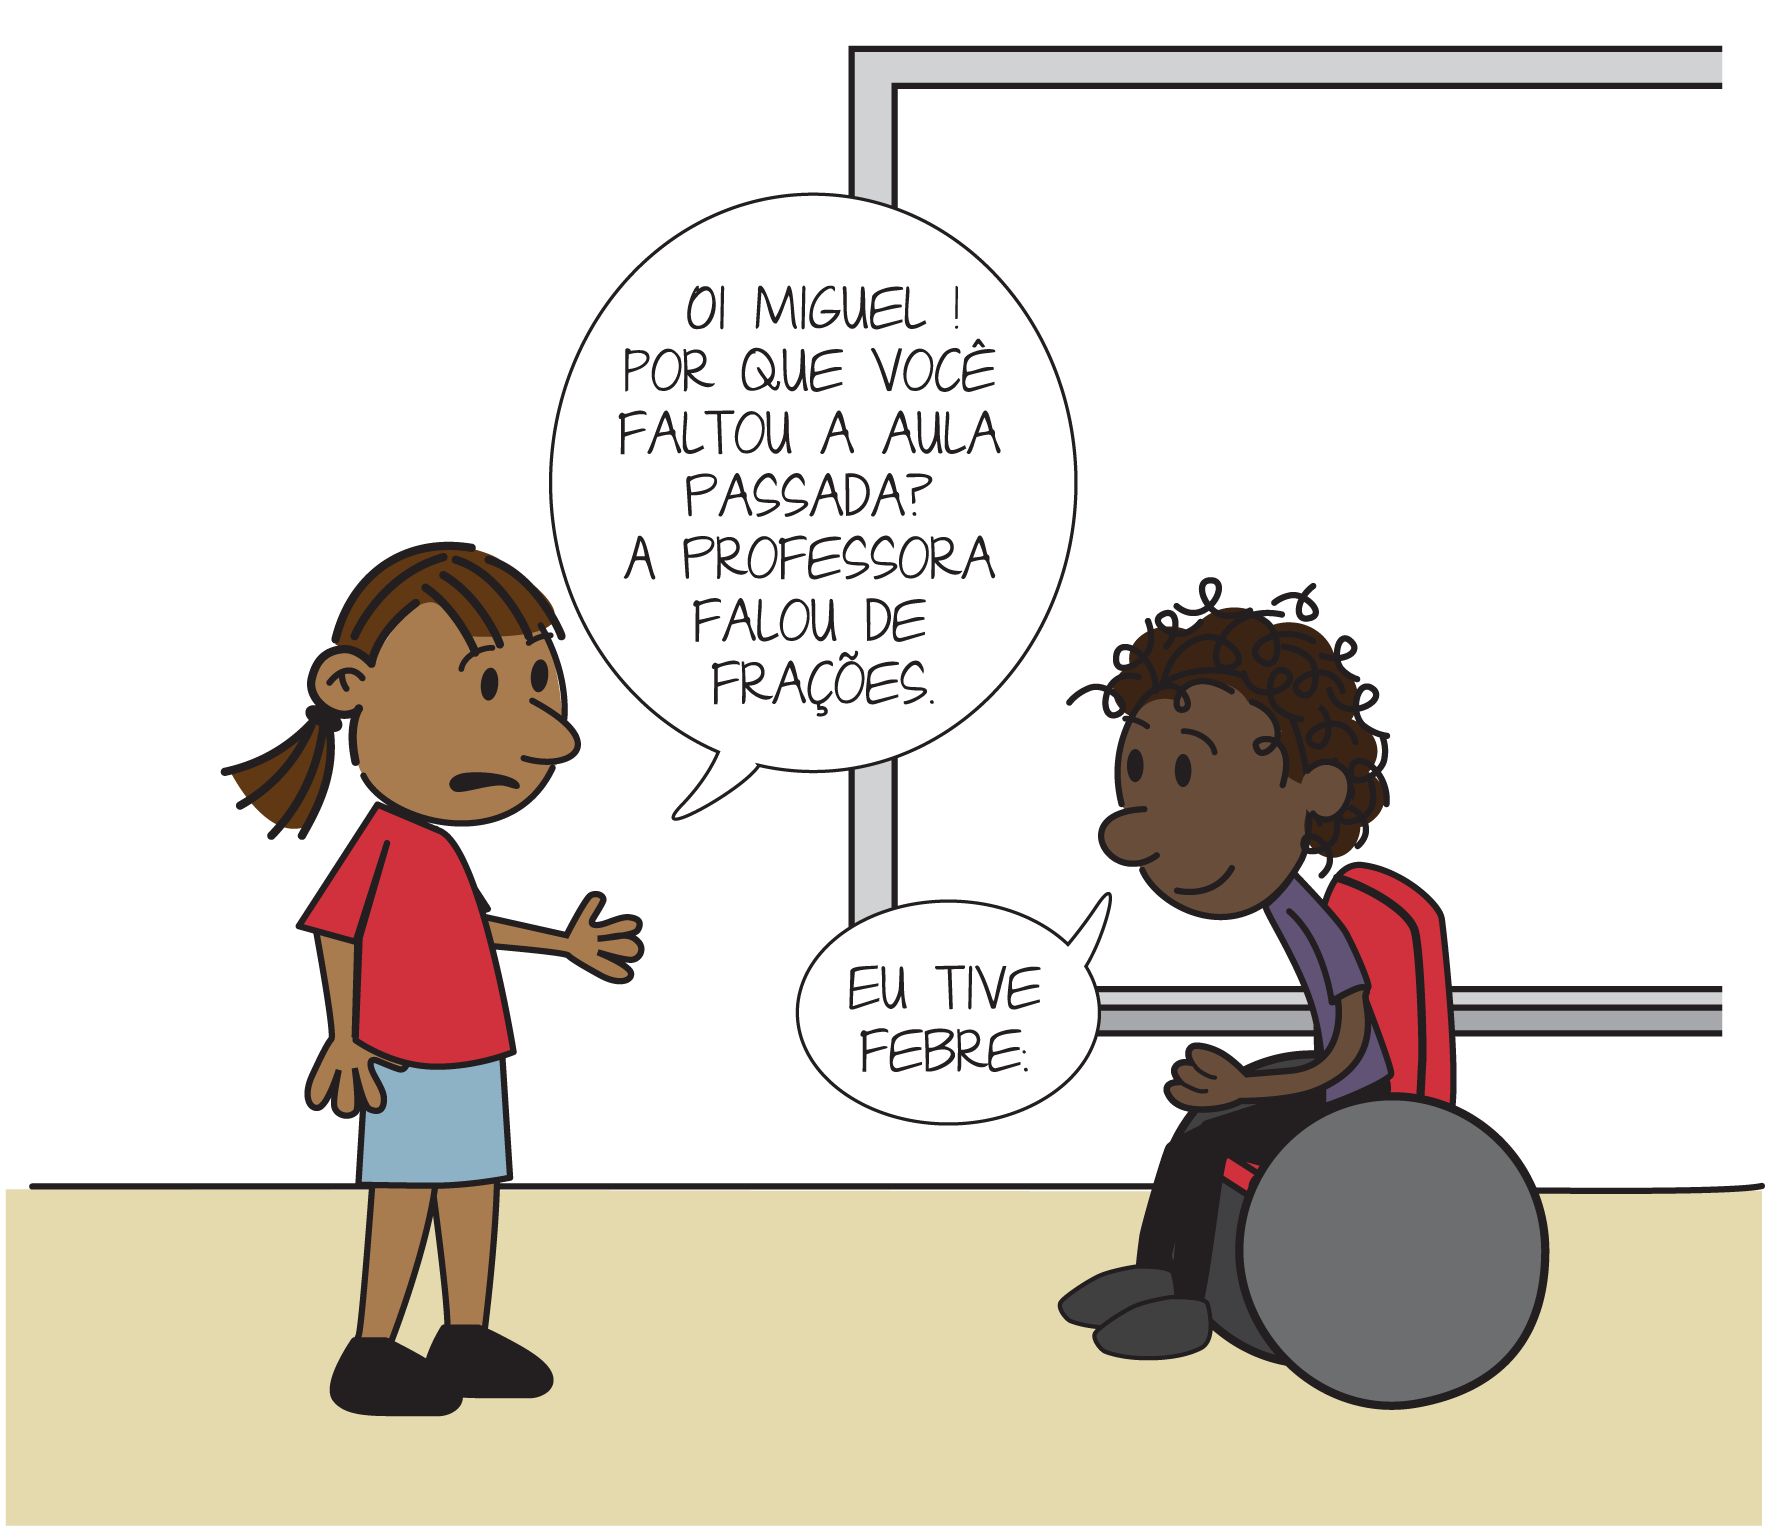
\includegraphics[width=.48\paperwidth, keepaspectratio]{licao02/quadrinho_01.png}   & 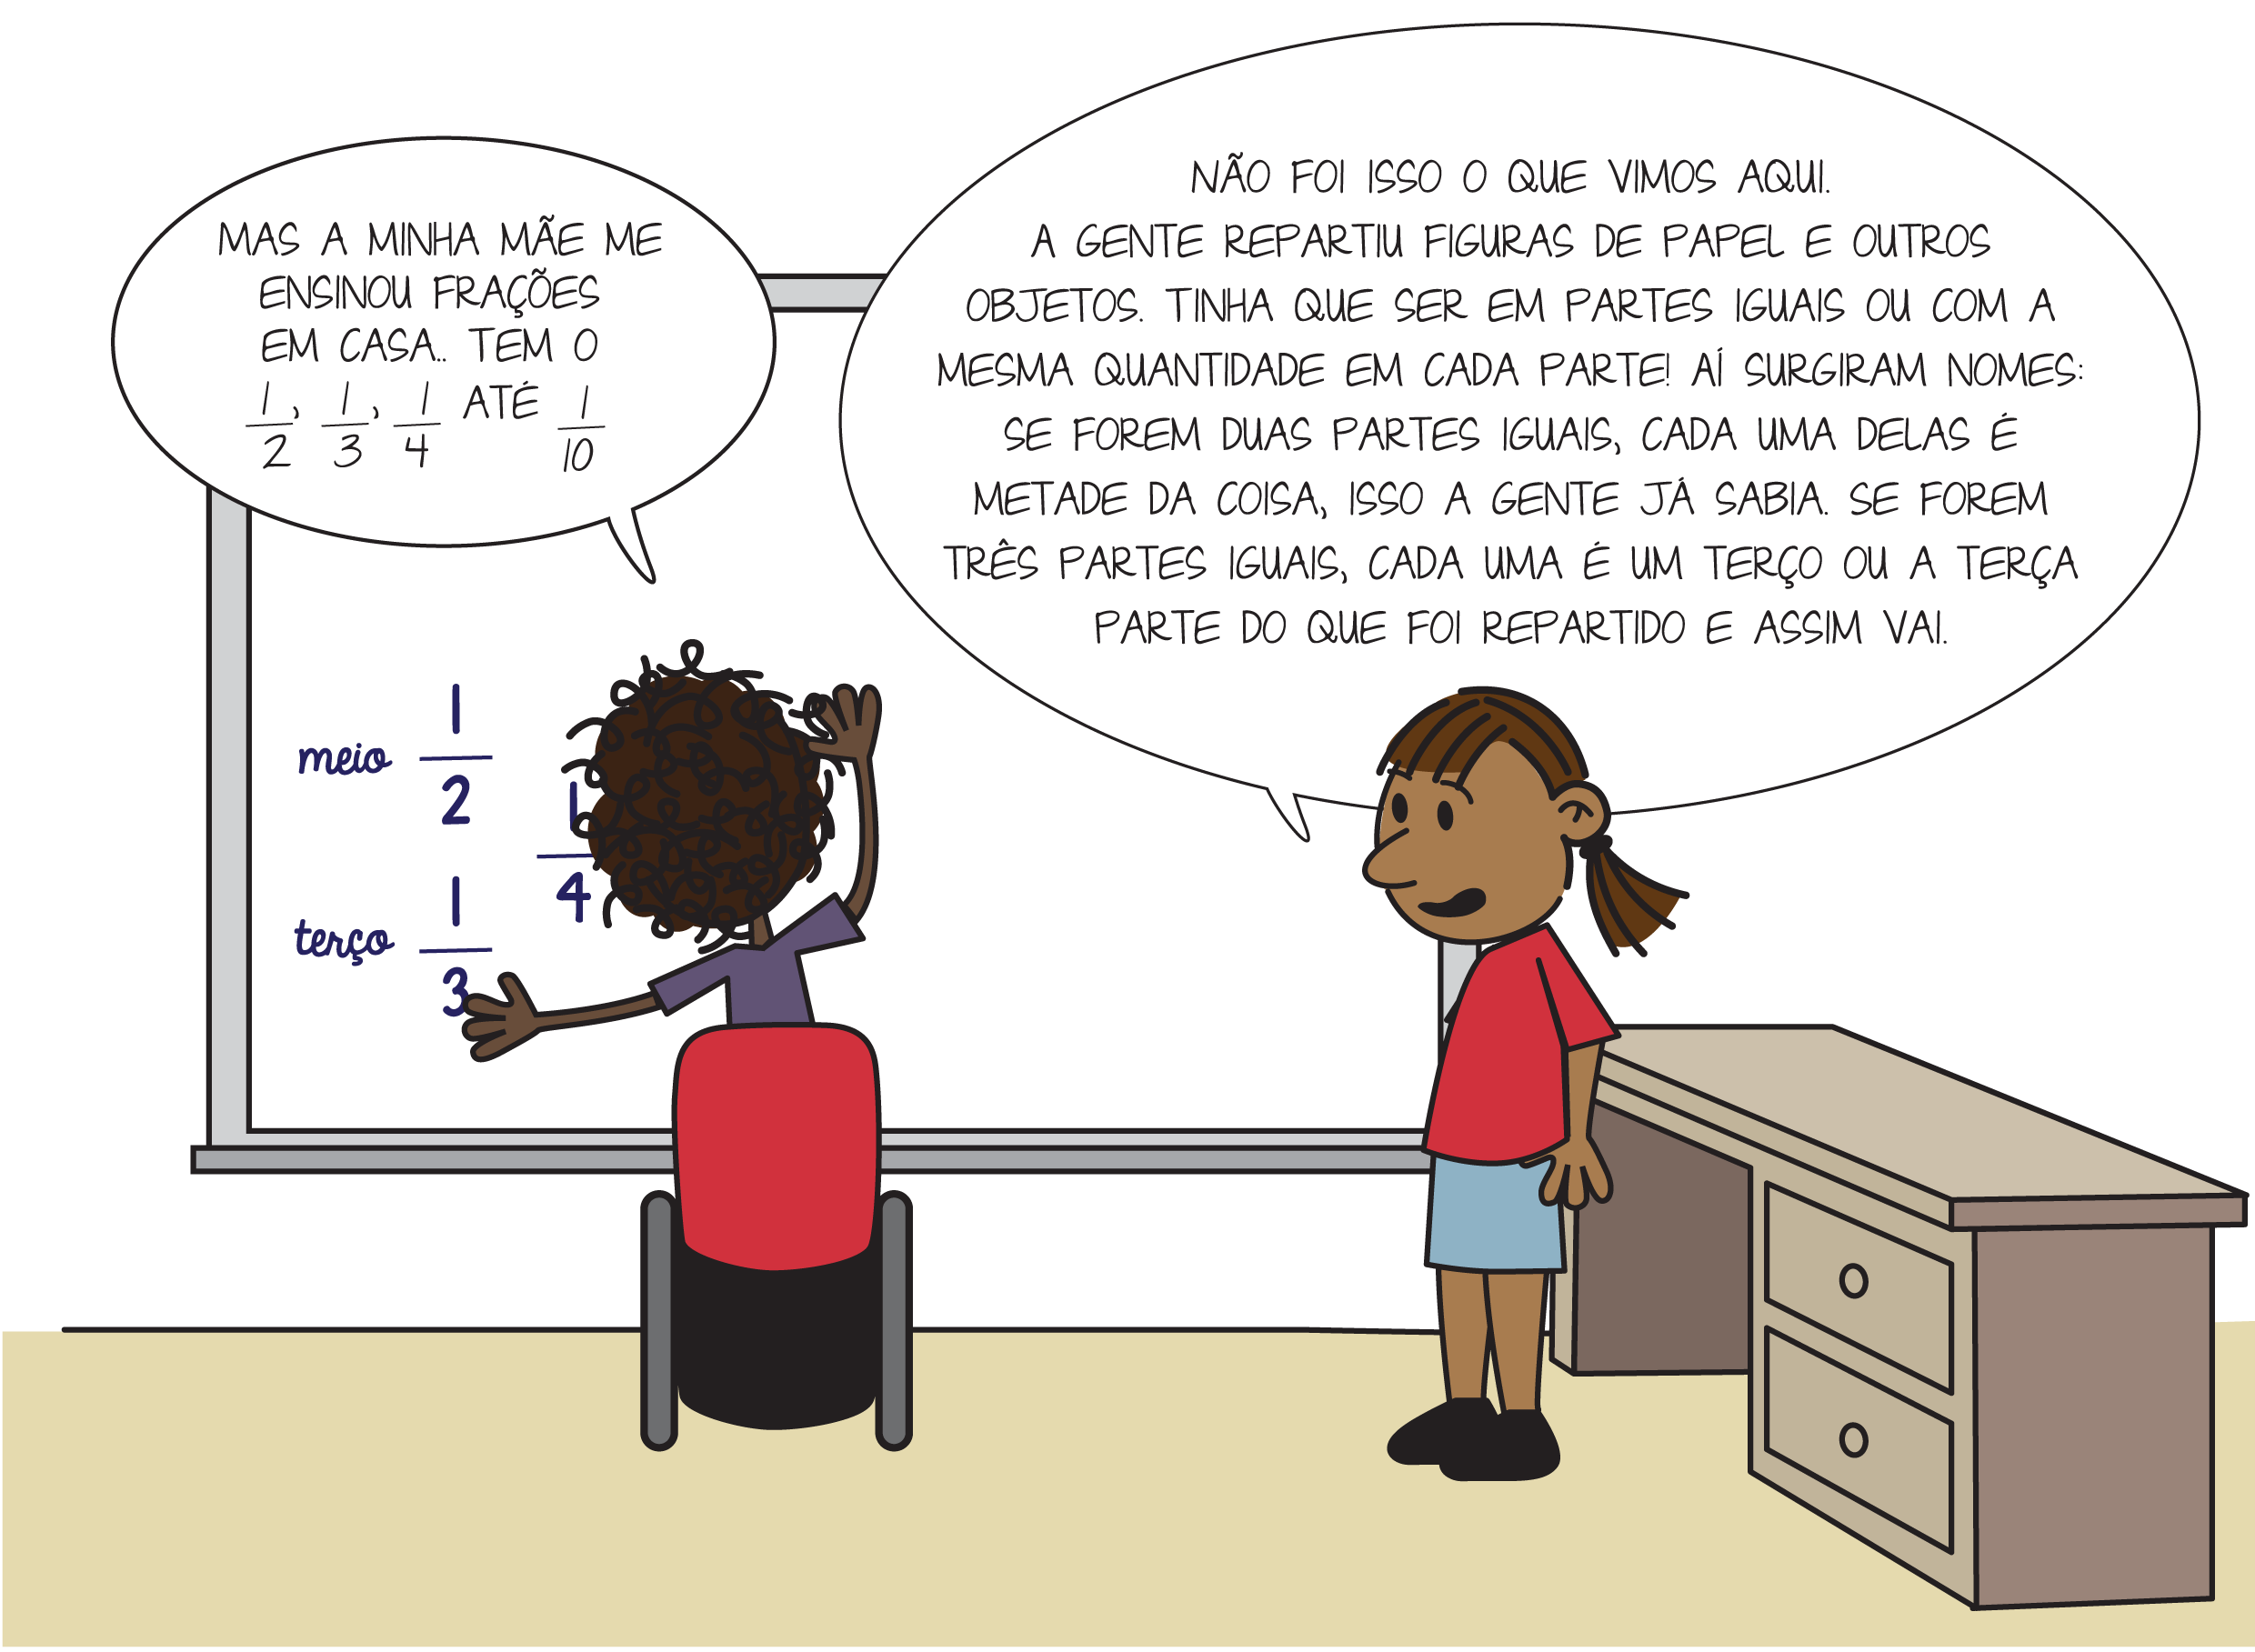
\includegraphics[width=.48\paperwidth, keepaspectratio]{licao02/quadrinho_02.png}   \\
 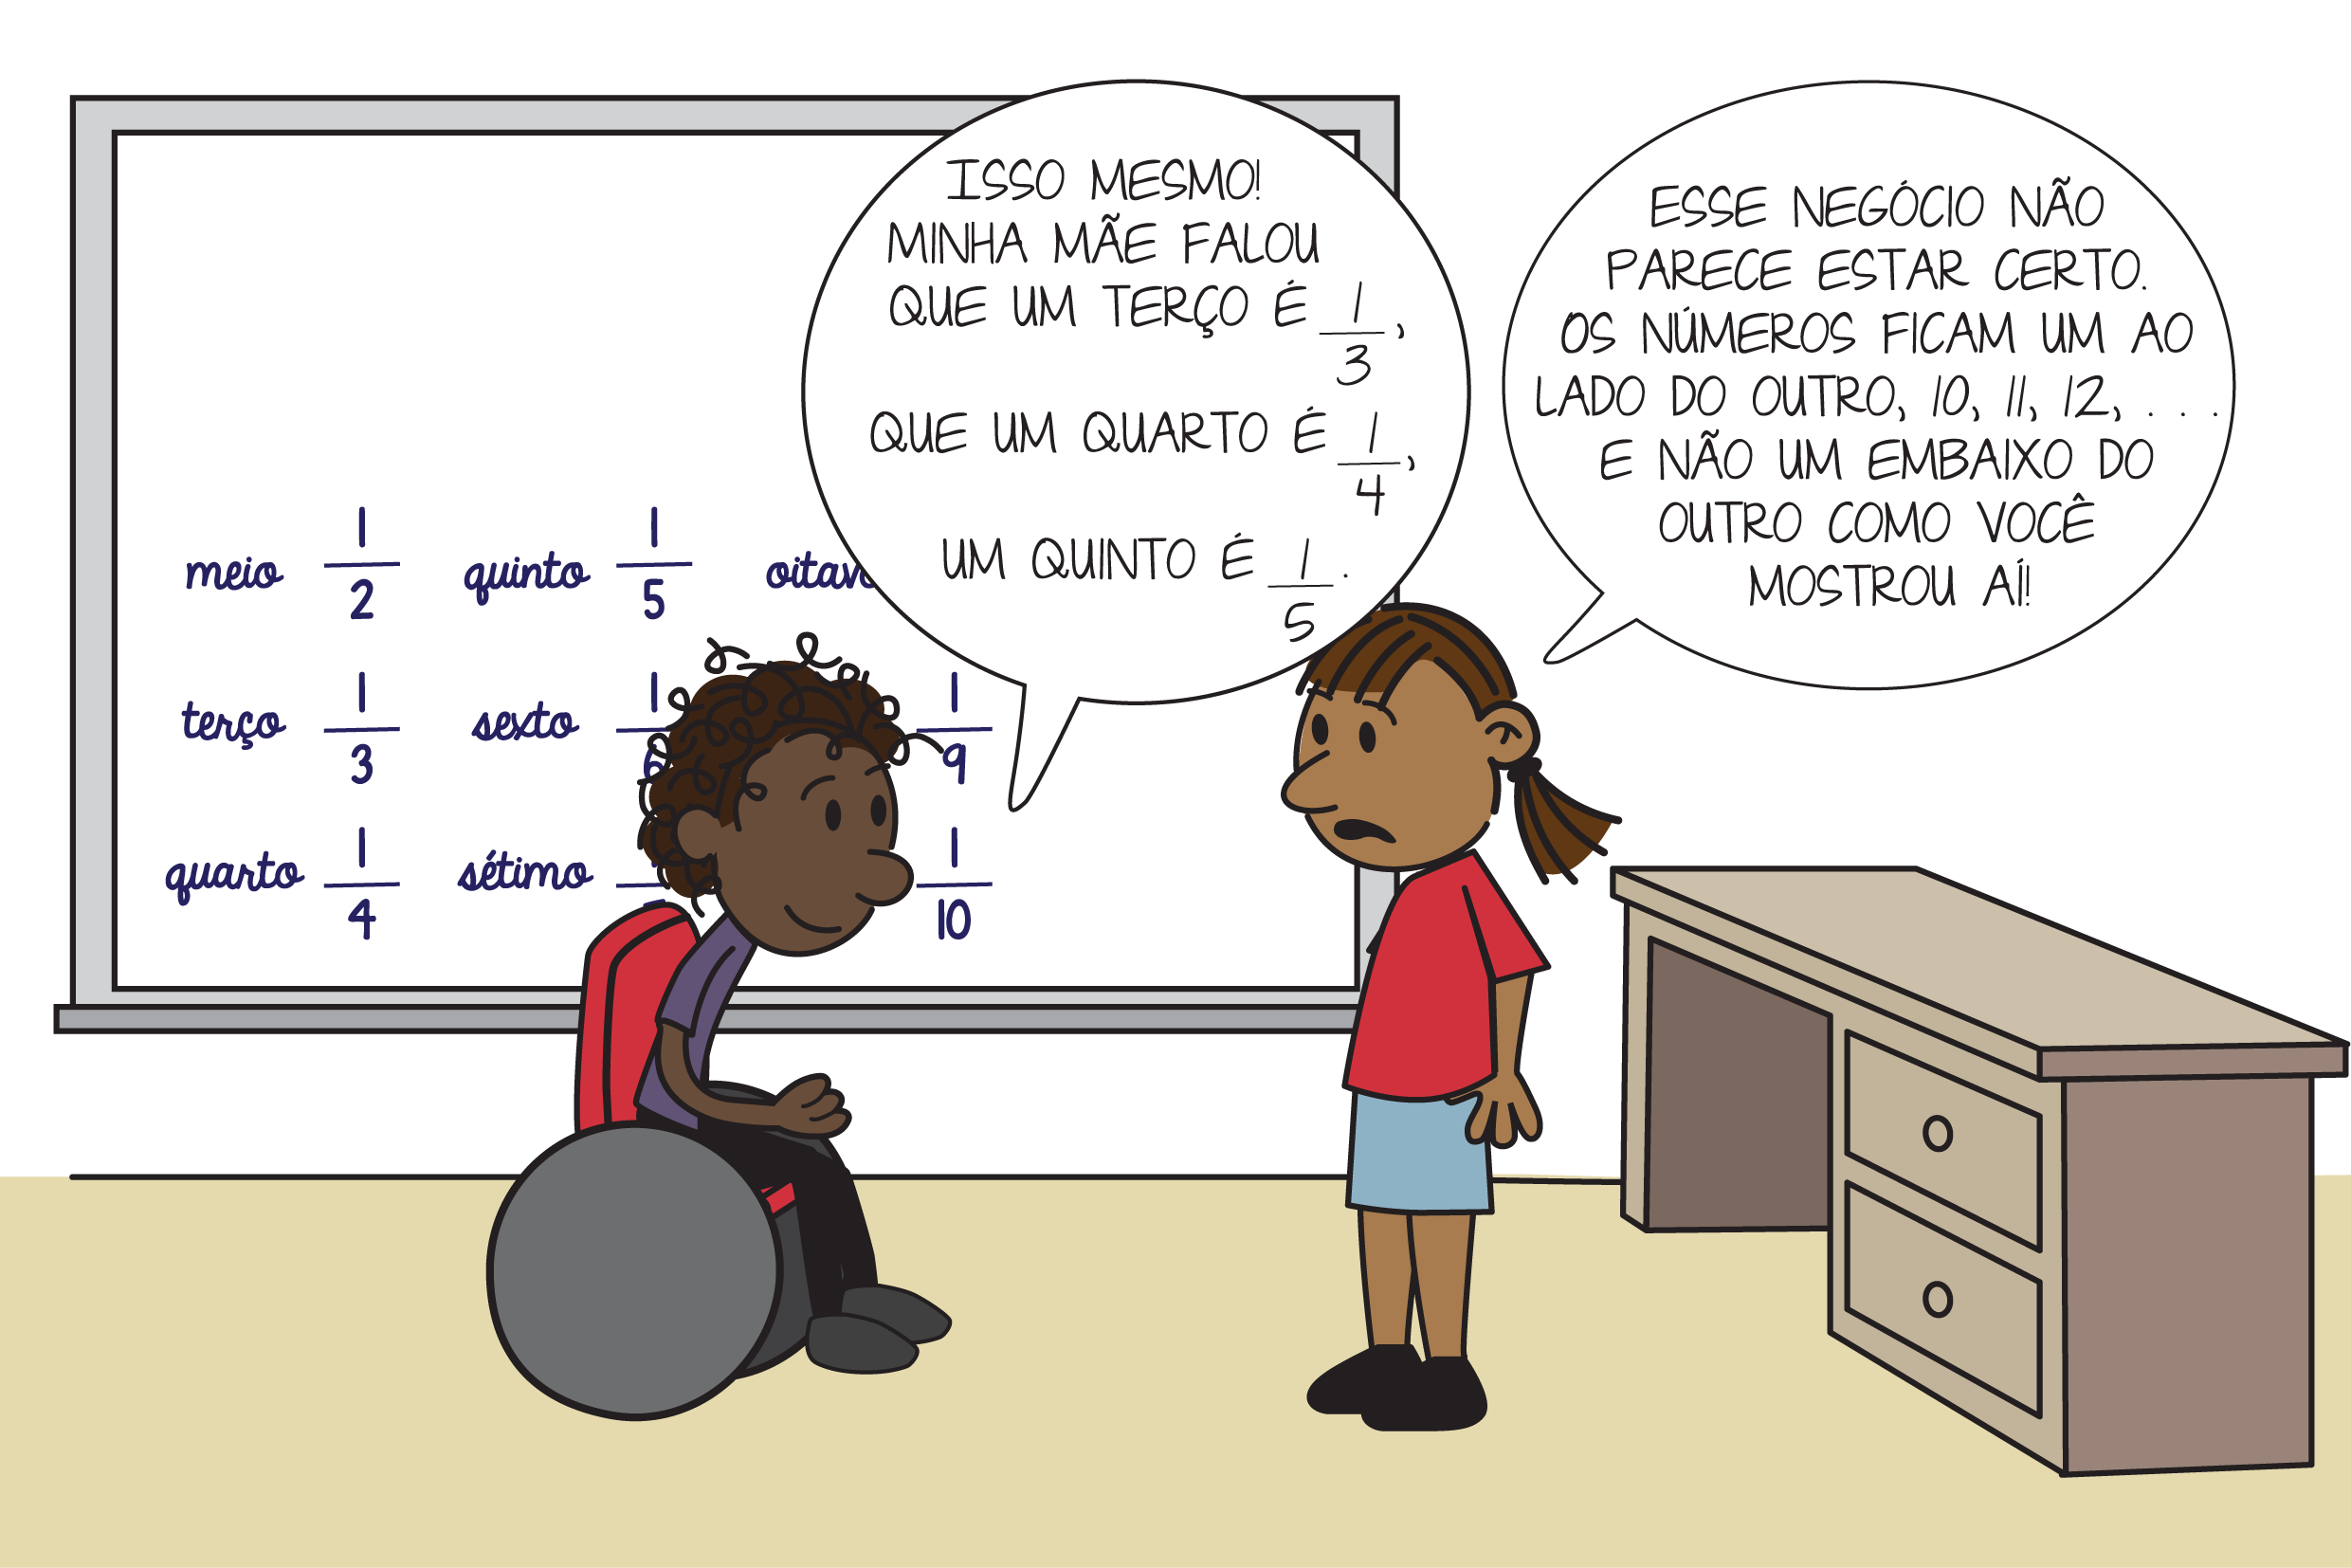
\includegraphics[width=.48\paperwidth, keepaspectratio]{licao02/quadrinho_03.png} & 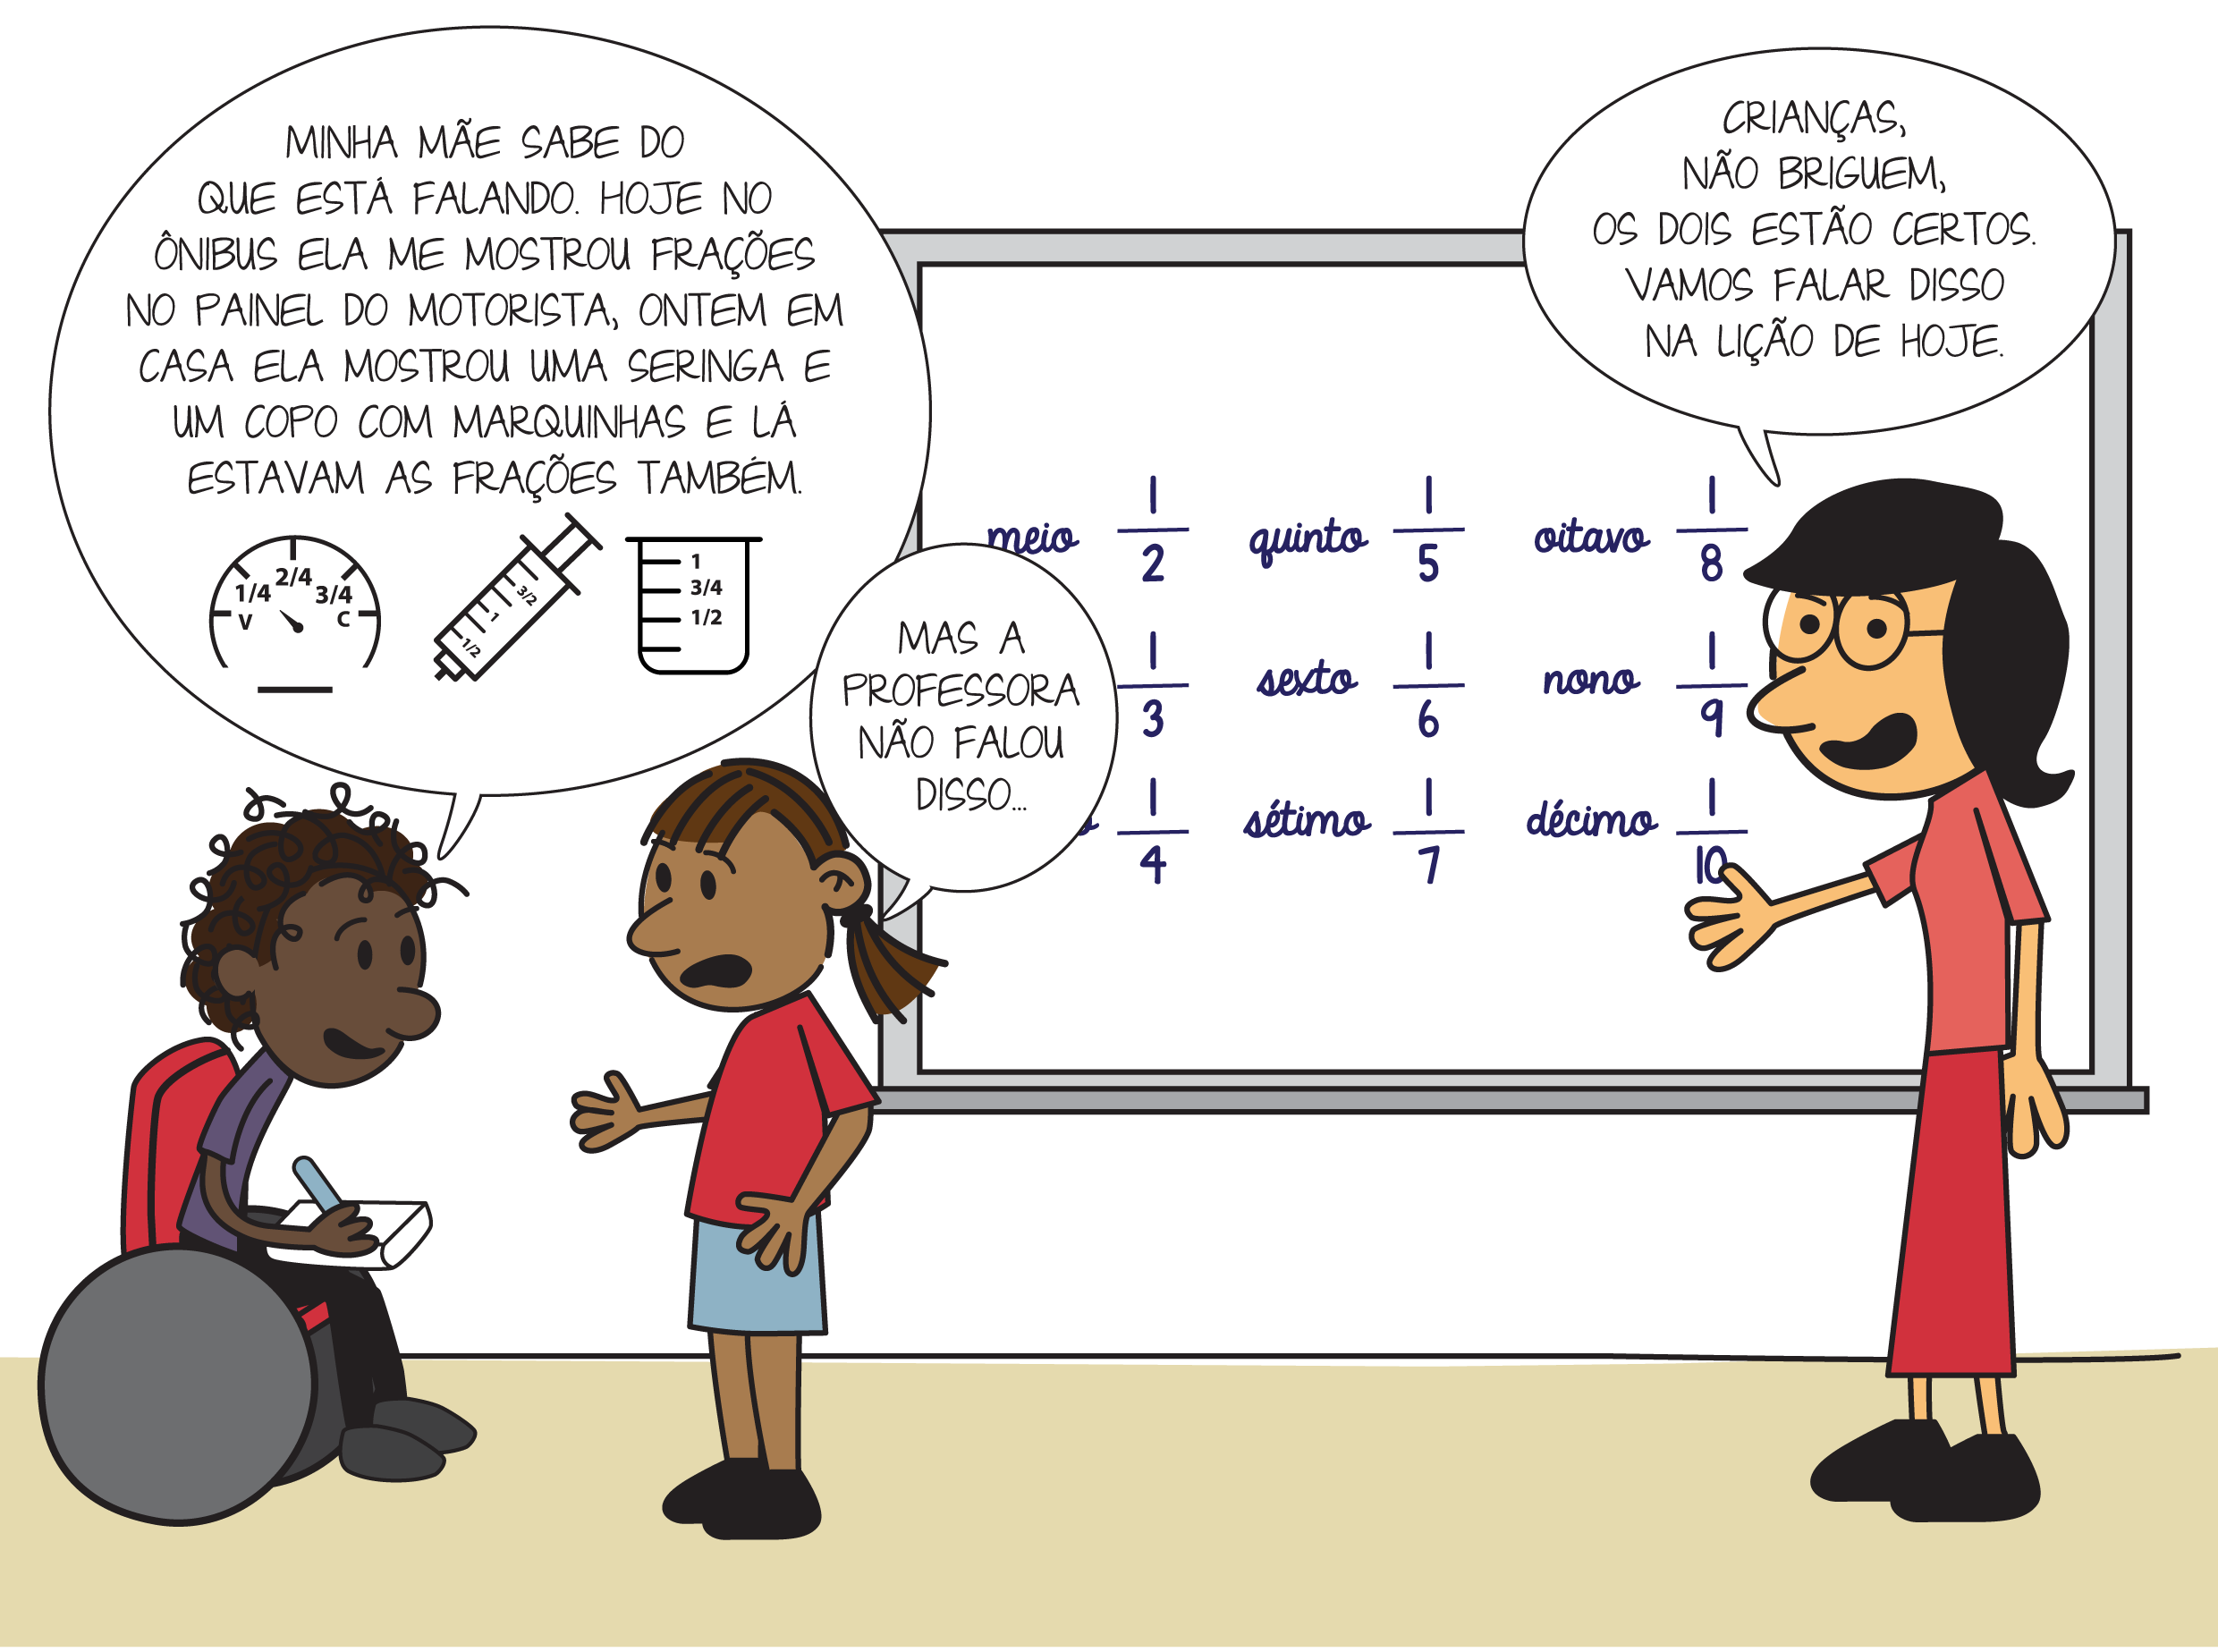
\includegraphics[width=.48\paperwidth, keepaspectratio]{licao02/quadrinho_04.png}
\end{tabular}


\clearpage

\section{EXPLORANDO O ASSUNTO }

\subsection{Atividade}

Luiza, João e Mariele foram a uma pizzaria. Cada um pediu uma pizza do seu sabor preferido. 
Luiza cortou sua pizza em 4 fatias; João cortou sua pizza em 6 fatias e Mariele cortou sua pizza em 8 fatias.
Veja o quanto restou de pizza após os amigos estarem satisfeitos:

\begin{center}
  \begin{tikzpicture}
\fill[common] (0,0) -- (120: 2cm) arc (120:240:2cm)--cycle;
\draw (0,0) circle (2cm);
\foreach \t in {0,60,...,300}{
  \draw (0,0) -- (\t: 2cm);
}  
\end{tikzpicture} \quad
\begin{tikzpicture}
\fill[common] (0,0) -- (135: 2cm) arc (135:225:2cm)--cycle;
\draw (0,0) circle (2cm);
\foreach \t in {0,45,...,315}{
  \draw (0,0) -- (\t: 2cm);
}  
\end{tikzpicture}\quad
\begin{tikzpicture}
\fill[common] (0,0) -- (180: 2cm) arc (180:270:2cm)--cycle;
\draw (0,0) circle (2cm);
\foreach \t in {0,90,...,270}{
  \draw (0,0) -- (\t: 2cm);
}  
\end{tikzpicture}
% Figura certa no Google Docs _Rascunho Frações
\end{center}

\begin{enumerate} [\quad a)] %d
\item   Identifique a pizza de cada um dos amigos.
\item   Em cada caso, que fração da pizza representa uma fatia?
\item   Escreva a quantidade de pizza que cada amigo comeu utilizando fração?
\end{enumerate}
 


\subsection{Atividade}

O pai de Ana, Beatriz e Clara trouxe duas barras de chocolate para serem repartidas entre elas.

\begin{center}
\begin{tikzpicture}[x=1mm,y=1mm, scale=0.9]
\draw[fill=Sepia] (0,0) rectangle (60,20);
\draw[fill=Sepia, shift={(65,0)}] (0,0) rectangle (60,20);
\end{tikzpicture}
\end{center}

Ana propôs que cada barra fosse dividida em três partes iguais e que cada irmã ficasse com duas dessas partes.

\begin{center}
\begin{tikzpicture}[x=1mm,y=1mm,scale=0.9]
\draw[fill=Sepia] (0,0) rectangle (60,20);
\draw (20,0) -- (20,20);
\draw (40,0) -- (40,20);

\draw[fill=Sepia, shift={(65,0)}] (0,0) rectangle (60,20);
\draw[shift={(65,0)}] (20,0) -- (20,20);
\draw[shift={(65,0)}] (40,0) -- (40,20);

\draw[very thick, shift={(62.5,-3)}, ->] (0,0) -- (0,-10);
\node at (90,-8) {Divisão sugerida por Ana};

\draw[fill=Sepia, shift={(-8.5,-36)}] (0,0) rectangle (20,20);
\draw[fill=Sepia, shift={(13.5,-36)}] (0,0) rectangle (20,20);

\draw[fill=Sepia, shift={(41.5,-36)}] (0,0) rectangle (20,20);
\draw[fill=Sepia, shift={(63.5,-36)}] (0,0) rectangle (20,20);

\draw[fill=Sepia, shift={(63.5 + 28,-36)}] (0,0) rectangle (20,20);
\draw[fill=Sepia, shift={(63.5 + 50,-36)}] (0,0) rectangle (20,20);

\draw [thick, decoration={brace,mirror,raise=5}, decorate] (-8.5,-36) -- (33.5,-36)
node [pos=0.5,anchor=north,yshift=-10] {\parbox[b]{40mm}{\centering Quantidade de chocolate recebida por Ana}};

\draw [thick, decoration={brace,mirror,raise=5}, decorate] (41.5,-36) -- (83.5,-36)
node [pos=0.5,anchor=north,yshift=-10] {\parbox[b]{40mm}{\centering Quantidade de chocolate recebida por Beatriz}};

\draw [thick, decoration={brace,mirror,raise=5}, decorate] (63.5+28,-36) -- (63.5+70,-36)
node [pos=0.5,anchor=north,yshift=-10] {\parbox[b]{40mm}{\centering Quantidade de chocolate recebida por Clara}};

\end{tikzpicture}
\end{center}

\begin{enumerate}[a)] %s
  \item Na divisão de cada uma das barras de chocolate em três partes iguais, cada parte é que fração de uma barra de chocolate?
  \item Você concorda com a divisão que Ana sugeriu? Explique.
  \item Com essa divisão, as três irmãs receberiam a mesma quantidade de chocolate?
  \item Na divisão proposta por Ana, como você nomearia, usando fração de uma barra de chocolate, a quantidade de chocolate que cada irmã receberia?
\end{enumerate}

Ana não quer o chocolate e decidiu dar a quantidade de chocolate que recebeu na divisão das barras para as suas irmãs.

\begin{enumerate}[e)]
\item Se Ana desse metade da quantidade de chocolate que recebeu para cada uma de suas irmãs, que quantidade de chocolate Beatriz e Clara passariam a ter? Como você nomearia, usando frações, essas quantidades?
\item[f)] E se Ana desse toda a quantidade de chocolate que recebeu para Beatriz, que quantidade de chocolate  Beatriz passaria a ter? Como você nomearia, usando frações, essa quantidade?
\end{enumerate} %s


\subsection{Atividade}

Um grupo de cinco amigos (Amarildo, Beto, Carlos, Davi e Edilson) encomendou três tortas salgadas, de mesmo tamanho retangular, como na ilustração para uma comemoração.

\begin{center}
 \begin{tikzpicture}[scale=0.6]
  \draw (0,0) rectangle (60,30);
  \draw (70,0) rectangle (130,30);
  \draw (140,0) rectangle (200,30);
 \end{tikzpicture}

\end{center}

\begin{enumerate} [\quad a)] %s
  \item     Como dividir as três tortas de modo que cada amigo receba a mesma quantidade de torta? Faça um desenho no seu caderno mostrando sua proposta de divisão. Indique qual parte é de qual amigo!
  \item     Considerando-se uma torta como unidade, como você nomearia, usando frações, a quantidade de torta que:
\begin{enumerate} [\quad I)] %d
      \item         Amarildo recebeu?
      \item         Amarildo e Beto receberam juntos?
      \item         Amarildo, Beto e Carlos receberam juntos?
      \item         Amarildo, Beto, Carlos e Davi receberam juntos?
      \item         Amarildo, Beto, Carlos, Davi e Edilson receberam juntos?
\end{enumerate} %d

  \item     A quantidade de torta que cada amigo recebeu é menor do que um quinto de torta? E do que dois quintos de torta? Explique sua resposta.
  \item     A quantidade de torta que cada amigo recebeu é maior do que três quintos de torta? E do que quatro quintos de torta? Explique sua resposta.
\end{enumerate} %s


\subsection{Atividade}

Para a sobremesa do almoço de domingo, papai passou em uma confeitaria que vende tortas divididas igualmente em 8 fatias, como na figura abaixo.
\begin{center}

\includegraphics[width=.6\textwidth, keepaspectratio]{licao02/ativ3_fig01.png}
\end{center}

\begin{enumerate} [\quad a)] %s
  \item     Que fração de uma torta é uma fatia? Explique.
  \item     Domingo papai comprou 4 fatias, quantos oitavos de uma torta havia para a sobremesa?
  \item     Na pergunta anterior, apresente outra fração que represente a quantidade de torta que papai comprou. Explique sua resposta.
  \item     Hoje papai comprou 10 fatias de torta. Como podemos representar essa quantidade de torta em termos de frações {\bf  de uma torta}? Lembre-se que oito fatias formam uma torta inteira.
\end{enumerate} %s

\subsection{Atividade}

Complete as afirmações com uma das frações: ``dois meios'', ``dois terços'', ``dois quintos'', ``três quartos'', ``oito sextos'' e ``nove meios'', para que sejam verdadeiras.

\begin{enumerate}[a)]
 \item A parte pintada de vermelho em \begin{tikzpicture}[scale=0.8]
                           \draw[fill=attention] (0,0) rectangle (20,10);
                           \draw[fill=common, fill opacity=.3] (20,0) rectangle (30,10);
                          \end{tikzpicture}
                          é \begin{tikzpicture}
                             \draw (0,0) -- (20,0);
                            \end{tikzpicture}
                            de \begin{tikzpicture}[scale=0.8]
                                 \draw[fill=common, fill opacity=.3] (0,0) rectangle (30,10);
                               \end{tikzpicture}.

 \item A parte pintada de vermelho em \begin{tikzpicture}
                           \draw[fill=attention] (0,0) rectangle (8,8);
                           \draw (0,0) -- (8,8);
                          \end{tikzpicture}
                          é \begin{tikzpicture}
                             \draw (0,0) -- (20,0);
                            \end{tikzpicture}
                            de \begin{tikzpicture}
                            \draw[fill=common, fill opacity=.3] (0,0) rectangle (8,8);
                           \end{tikzpicture}.


 \item A parte pintada de vermelho em \begin{tikzpicture}
                           \draw[fill=common, fill opacity=.3] (0,0) circle (4);
                           \fill[attention] (0,0) -- (72:4) arc (72:-72:4) --cycle;
                           \foreach \x in {0,72,...,288}{
                           \draw (0,0) -- (\x:4);}
                          \end{tikzpicture}
                          é \begin{tikzpicture}
                             \draw (0,0) -- (20,0);
                            \end{tikzpicture}
                            de \begin{tikzpicture}
                            \draw[fill=common, fill opacity=.3] (0,0) circle (4);
                           \end{tikzpicture}.

 \item A parte pintada de vermelho em \begin{tikzpicture}
                                       \fill[attention]  \foreach \x/\y in {36/72,108/144,180/212, 252/284, 324/360}{ (0,0) -- (\x-18:4) -- (\y-18:2)--(\x-18 +72:4) -- (0, 0)};
                                       \draw  \foreach \x/\y in {36/72,108/144,180/212, 252/284, 324/360}{ (\x-18:4) -- (\y-18:2)--(\x-18 +72:4)};
                                      \end{tikzpicture} \begin{tikzpicture}
                                       \fill[attention]  \foreach \x/\y in {36/72,108/144,180/212, 252/284, 324/360}{ (0,0) -- (\x-18:4) -- (\y-18:2)--(\x-18 +72:4) -- (0, 0)};
                                       \draw  \foreach \x/\y in {36/72,108/144,180/212, 252/284, 324/360}{ (\x-18:4) -- (\y-18:2)--(\x-18 +72:4)};
                                      \end{tikzpicture} \begin{tikzpicture}
                                       \fill[attention]  \foreach \x/\y in {36/72,108/144,180/212, 252/284, 324/360}{ (0,0) -- (\x-18:4) -- (\y-18:2)--(\x-18 +72:4) -- (0, 0)};
                                       \draw  \foreach \x/\y in {36/72,108/144,180/212, 252/284, 324/360}{ (\x-18:4) -- (\y-18:2)--(\x-18 +72:4)};
                                      \end{tikzpicture} \begin{tikzpicture}
                                       \fill[attention]  \foreach \x/\y in {36/72,108/144,180/212, 252/284, 324/360}{ (0,0) -- (\x-18:4) -- (\y-18:2)--(\x-18 +72:4) -- (0, 0)};
                                       \draw  \foreach \x/\y in {36/72,108/144,180/212, 252/284, 324/360}{ (\x-18:4) -- (\y-18:2)--(\x-18 +72:4)};
                                      \end{tikzpicture} \begin{tikzpicture}
                                       \fill[attention]  \foreach \x/\y in {36/72,108/144,180/212, 252/284, 324/360}{ (0,0) -- (\x-18:4) -- (\y-18:2)--(\x-18 +72:4) -- (0, 0)};
                                       \fill[white]  (90:4) -- (-90:2) -- (-56:4) -- (-18:2)-- (18:4) --(56:2) --cycle;
                                       \fill[common, opacity=.3]  (90:4) -- (-90:2) -- (-56:4) -- (-18:2)-- (18:4) --(56:2) --cycle;
                                       \draw  \foreach \x/\y in {36/72,108/144,180/212, 252/284, 324/360}{ (\x-18:4) -- (\y-18:2)--(\x-18 +72:4)};
                                      \end{tikzpicture} é \begin{tikzpicture} \draw (0,0) -- (20,0); \end{tikzpicture} de \begin{tikzpicture}
                                       \fill[common, opacity=.3]  \foreach \x/\y in {36/72,108/144,180/212, 252/284, 324/360}{ (0,0) -- (\x-18:4) -- (\y-18:2)--(\x-18 +72:4) -- (0, 0)};
                                       \draw  \foreach \x/\y in {36/72,108/144,180/212, 252/284, 324/360}{ (\x-18:4) -- (\y-18:2)--(\x-18 +72:4)};
                                      \end{tikzpicture}.

\item A parte pintada de vermelho em \begin{tikzpicture} \draw[fill=attention] (90:4)--(-90:4)--(-30:4)--(30:4)--cycle; \foreach \x in {30,90,...,330}{\draw (0,0) -- (\x:4);} \draw[fill=common, fill opacity=.3] (90:4) -- (150:4) -- (210:4) -- (270:4) -- cycle;\end{tikzpicture} \begin{tikzpicture} \fill[attention] (30:4)--(90:4)--(150:4)--(210:4)--(270:4)-- (330:4) -- (0,0) --cycle; \foreach \x in {30,90,...,330}{\draw (0,0) -- (\x:4); \draw (\x:4) -- (\x+60:4);} \fill[common, fill opacity=.3] (0,0) -- (30:4) -- (-30:4) -- cycle;\end{tikzpicture} é \begin{tikzpicture} \draw (0,0) -- (20,0); \end{tikzpicture} de \begin{tikzpicture} \draw[fill=common, fill opacity=.3] (30:4) --(90:4)--(150:4)--(210:4)--(270:4)-- (330:4) -- cycle;\end{tikzpicture}.
\end{enumerate}

\section{ORGANIZANDO AS IDEIAS }

Se uma torta está dividida em três partes iguais, a torta fica separada em três terços. Assim, como visto na historinha do início da lição, tanto faz escrever: ``$\frac{1}{3}$ da torta'' ou ``um terço da torta'' para se referir à fatia destacada na figura.

\begin{center}
\begin{tikzpicture}
 \draw[fill=common, fill opacity=.3] (0,0) circle (10);
 \draw[fill=attention] (0,0) -- (-90:10) arc (-90:30:10) -- (0,0) -- cycle;
 \draw (0,0) -- (-90:10);
 \draw (0,0) -- (30:10);
 \draw (0,0) -- (150:10);
 \node at (0,-14) {$\frac{1}{3}$ da torta};
\end{tikzpicture}
\end{center}


Duas fatias são ``dois terços da torta'', o que pode ser expresso simplesmente por ``$\frac{2}{3}$ da torta''. Deste modo, ``três terços da torta'' é uma torta inteira.

\begin{center}
\begin{tikzpicture}
 \draw[fill=common, fill opacity=.3] (0,0) circle (10);
 \draw[fill=attention] (0,0) -- (-210:10) arc (-210:30:10) -- (0,0) -- cycle;
 \draw (0,0) circle (10);
 \draw (0,0) -- (-90:10);
 \draw (0,0) -- (30:10);
 \draw (0,0) -- (150:10);
 \node at (0,-14) {$\frac{2}{3}$ da torta};
\end{tikzpicture}\quad \quad \quad \begin{tikzpicture}
 \draw[fill=attention] (0,0) circle (10);
 \draw (0,0) -- (-90:10);
 \draw (0,0) -- (30:10);
 \draw (0,0) -- (150:10);
 \node at (0,-14) {$\frac{3}{3}$ da torta};
\end{tikzpicture}
\end{center}


Também pode-se considerar quatro terços, cinco terços ou seis terços da torta, basta juntar novos terços à torta inteira.

\begin{center}
\begin{tikzpicture}
\begin{scope}[shift={(-24,0)}]
 \draw[fill=attention] (0,0) circle (10);
 \draw (0,0) -- (-90:10);
 \draw (0,0) -- (30:10);
 \draw (0,0) -- (150:10);
 \end{scope}
 \draw[fill=attention] (0,0) -- (150:10) arc (150:30:10) -- (0,0) -- cycle;
 \node at (-12,-14) {$\frac{4}{3}$ da torta = 1 torta e $\frac{1}{3}$ da torta};
\end{tikzpicture}
\vspace{0.4cm}

\begin{tikzpicture}
\begin{scope}[shift={(-24,0)}]
 \draw[fill=attention] (0,0) circle (10);
 \draw (0,0) -- (-90:10);
 \draw (0,0) -- (30:10);
 \draw (0,0) -- (150:10);
 \end{scope}
 \draw[fill=attention] (0,0) -- (150:10) arc (150:-90:10) -- (0,0) -- cycle;
 \draw (0,0) -- (30:10);
 \node at (-12,-14) {$\frac{5}{3}$ da torta = 1 torta e $\frac{2}{3}$ da torta};
\end{tikzpicture}
\vspace{0.4cm}

\begin{tikzpicture}
\begin{scope}[shift={(-24,0)}]
 \draw[fill=attention] (0,0) circle (10);
 \draw (0,0) -- (-90:10);
 \draw (0,0) -- (30:10);
 \draw (0,0) -- (150:10);
 \end{scope}
 \draw[fill=attention] (0,0) circle (10);
 \draw (0,0) -- (-90:10);
 \draw (0,0) -- (30:10);
 \draw (0,0) -- (150:10);
 \node at (-12,-14) {$\frac{6}{3}$ da torta = 2 tortas};
\end{tikzpicture}
\end{center}

Se uma torta é repartida em três partes iguais, cada fatia é um terço da torta - ou, simplesmente, $\frac{1}{3}$ da torta. Juntando essas fatias, é possível se ter dois terços ($\frac{2}{3}$) e três terços ($\frac{3}{3}$) da torta. Com mais do que uma torta repartida em três partes iguais, pode-se obter quatro terços ($\frac{4}{3}$), cinco terços ($\frac{5}{3}$), seis terços ($\frac{6}{3}$) etc de torta. Na representação simbólica, as frações que registram essas quantidades têm o número 3 ``abaixo'' do traço de fração, e, por isso, são denominadas terços. O número que informa a parte da unidade que ``dá nome'' à fração é chamado de {\it denominador} da fração. Assim, nas frações $\frac{1}{3}$, $\frac{2}{3}$, $\frac{3}{3}$,  $\frac{4}{3}$ e $\frac{5}{3}$, o 3 é o denominador, identificando ``terços''.

Já o número que aparece ``acima'' do traço de fração informa quantos terços estão sendo considerados. Esse número é chamado de {\it numerador} da fração. Por exemplo, na fração $\frac{1}{3}$ o numerador é 1 e na fração $\frac{4}{3}$ o numerador é 4.

Essa mesma forma de nomear vale para outras frações, mesmo que o denominador seja diferente de 3: \newline
Em $\frac{2}{5}$, por exemplo, o numerador é 2 e o denominador é 5. Lê-se {\it dois quintos}.\newline
Em $\frac{10}{8}$, por exemplo, o numerador é 10 e o denominador é 8. Lê-se {\it dez oitavos}. \newline
Como você pôde observar, a nomeação de uma fração depende fortemente do denominador da fração. Para ler a fração deve-se ler o {\bf número} do numerador seguido do {\bf nome que identifica a equipartição da unidade, e que está indicado no denominador}, nessa ordem. Veja:

$$\frac{1}{3}\rightarrow \text{ um terço;} \quad \frac{2}{3}\rightarrow \text{ dois terços;} \quad \frac{5}{3}\rightarrow \text{ cinco terços;}$$
$$\frac{1}{8}\rightarrow \text{ um oitavo;} \quad \frac{3}{8}\rightarrow \text{ três oitavos;} \quad \frac{7}{8}\rightarrow \text{ sete oitavos.}$$
Anote agora os nomes de algumas outras frações:
$$\frac{1}{2}\rightarrow \text{  um meio;} \quad \frac{1}{3}\rightarrow\text{  um terço;} \quad \frac{1}{4}\rightarrow\text{  um quarto;}$$
$$\frac{1}{5}\rightarrow\text{  um quinto;}\quad \frac{1}{6}\rightarrow\text{  um sexto;} \quad \frac{1}{7}\rightarrow\text{  um sétimo;}$$
$$\frac{1}{8}\rightarrow\text{  um oitavo;}\quad \frac{1}{9}\rightarrow\text{  um nono;}\quad \frac{1}{10}\rightarrow\text{  um décimo.}$$

Para a fração $\frac{1}{11}$, fala-se um onze avos. Da mesma forma, são nomeadas frações cujo denominador é maior do que 11. Por exemplo:
$$\frac{1}{12}\rightarrow \text{  um doze avos;}\quad \frac{1}{13}\rightarrow \text{ um treze avos;} \quad \frac{5}{13}\rightarrow \text{ cinco treze avos.}$$

Curioso para saber sobre o significado da palavra {\bf avos}? Pergunte ao seu professor. O importante é lembrar que, para denominadores maiores 11, acrescenta-se a expressão ``avos'' ao final da leitura da fração.

Contudo, para frações cujo denominador é uma potência de 10, usa-se outra formar de ler:
$$\frac{1}{100}\rightarrow \text{ um centésimo;}\quad \frac{13}{100} \rightarrow \text{treze centésimos;} \quad
\frac{33}{1000}\rightarrow \text{ trinta e três milésimos.}$$

{\bf Pronto! Agora você já é capaz de ler diversos tipos de frações.}

\begin{center}
 
\includegraphics[width=.9\textwidth, keepaspectratio]{licao02/orgideias_fig01.png}
\end{center}


\section{MÃO NA MASSA }

\subsection{Atividade}

Uma pizza gigante foi dividida em doze fatias iguais.
Pedro comeu quatro fatias, Isabella cinco fatias, Bernardo duas fatias e Manuela apenas uma fatia.

\begin{center}
  \begin{tabular}{|m{0.27\textwidth}|m{0.13\textwidth}|m{0.13\textwidth}|m{0.13\textwidth}|m{0.13\textwidth}|}
\hline
& \centering Pedro & \centering  Isabella & \centering  Bernardo &  \quad Manuela  \\
    \hline  \hline
   Pinte a fração de pizza consumida  por cada pessoa      & \parbox[c][2cm]{0.13\textwidth}{\centering \begin{tikzpicture}[x=1.0cm,y=1.0cm, scale=0.5]
\draw (1.76,2.04) circle (1.78cm);
\draw [shift={(1.76,2.04)}]  (0,0) --  plot[domain=0.:0.5235987755982987,variable=\t]({1.*1.78*cos(\t r)+0.*1.78*sin(\t r)},{0.*1.78*cos(\t r)+1.*1.78*sin(\t r)}) -- cycle ;
\draw [shift={(1.76,2.04)}]  (0,0) --  plot[domain=0.5235987755982987:1.0471975511965974,variable=\t]({1.*1.78*cos(\t r)+0.*1.78*sin(\t r)},{0.*1.78*cos(\t r)+1.*1.78*sin(\t r)}) -- cycle ;
\draw [shift={(1.76,2.04)}]  (0,0) --  plot[domain=1.0471975511965974:1.5707963267948963,variable=\t]({1.*1.78*cos(\t r)+0.*1.78*sin(\t r)},{0.*1.78*cos(\t r)+1.*1.78*sin(\t r)}) -- cycle ;
\draw [shift={(1.76,2.04)}]  (0,0) --  plot[domain=1.5707963267948963:2.0943951023931953,variable=\t]({1.*1.78*cos(\t r)+0.*1.78*sin(\t r)},{0.*1.78*cos(\t r)+1.*1.78*sin(\t r)}) -- cycle ;
\draw [shift={(1.76,2.04)}]  (0,0) --  plot[domain=2.0943951023931953:2.617993877991494,variable=\t]({1.*1.78*cos(\t r)+0.*1.78*sin(\t r)},{0.*1.78*cos(\t r)+1.*1.78*sin(\t r)}) -- cycle ;
\draw [shift={(1.76,2.04)}]  (0,0) --  plot[domain=2.617993877991494:3.1415926535897927,variable=\t]({1.*1.78*cos(\t r)+0.*1.78*sin(\t r)},{0.*1.78*cos(\t r)+1.*1.78*sin(\t r)}) -- cycle ;
\draw [shift={(1.76,2.04)}]  (0,0) --  plot[domain=3.1415926535897927:3.6651914291880914,variable=\t]({1.*1.78*cos(\t r)+0.*1.78*sin(\t r)},{0.*1.78*cos(\t r)+1.*1.78*sin(\t r)}) -- cycle ;
\draw [shift={(1.76,2.04)}]  (0,0) --  plot[domain=3.6651914291880914:4.18879020478639,variable=\t]({1.*1.78*cos(\t r)+0.*1.78*sin(\t r)},{0.*1.78*cos(\t r)+1.*1.78*sin(\t r)}) -- cycle ;
\draw [shift={(1.76,2.04)}]  (0,0) --  plot[domain=4.18879020478639:4.712388980384689,variable=\t]({1.*1.78*cos(\t r)+0.*1.78*sin(\t r)},{0.*1.78*cos(\t r)+1.*1.78*sin(\t r)}) -- cycle ;
\draw [shift={(1.76,2.04)}]  (0,0) --  plot[domain=4.712388980384689:5.235987755982988,variable=\t]({1.*1.78*cos(\t r)+0.*1.78*sin(\t r)},{0.*1.78*cos(\t r)+1.*1.78*sin(\t r)}) -- cycle ;
\draw [shift={(1.76,2.04)}]  (0,0) --  plot[domain=5.235987755982988:5.759586531581286,variable=\t]({1.*1.78*cos(\t r)+0.*1.78*sin(\t r)},{0.*1.78*cos(\t r)+1.*1.78*sin(\t r)}) -- cycle ;
\draw [shift={(1.76,2.04)}]  (0,0) --  plot[domain=-0.5235987755983:0.,variable=\t]({1.*1.78*cos(\t r)+0.*1.78*sin(\t r)},{0.*1.78*cos(\t r)+1.*1.78*sin(\t r)}) -- cycle ;
\end{tikzpicture}}
  & \parbox[c][2cm]{0.13\textwidth}{\centering \begin{tikzpicture}[x=1.0cm,y=1.0cm, scale=0.5]
\draw (1.76,2.04) circle (1.78cm);
\draw [shift={(1.76,2.04)}]  (0,0) --  plot[domain=0.:0.5235987755982987,variable=\t]({1.*1.78*cos(\t r)+0.*1.78*sin(\t r)},{0.*1.78*cos(\t r)+1.*1.78*sin(\t r)}) -- cycle ;
\draw [shift={(1.76,2.04)}]  (0,0) --  plot[domain=0.5235987755982987:1.0471975511965974,variable=\t]({1.*1.78*cos(\t r)+0.*1.78*sin(\t r)},{0.*1.78*cos(\t r)+1.*1.78*sin(\t r)}) -- cycle ;
\draw [shift={(1.76,2.04)}]  (0,0) --  plot[domain=1.0471975511965974:1.5707963267948963,variable=\t]({1.*1.78*cos(\t r)+0.*1.78*sin(\t r)},{0.*1.78*cos(\t r)+1.*1.78*sin(\t r)}) -- cycle ;
\draw [shift={(1.76,2.04)}]  (0,0) --  plot[domain=1.5707963267948963:2.0943951023931953,variable=\t]({1.*1.78*cos(\t r)+0.*1.78*sin(\t r)},{0.*1.78*cos(\t r)+1.*1.78*sin(\t r)}) -- cycle ;
\draw [shift={(1.76,2.04)}]  (0,0) --  plot[domain=2.0943951023931953:2.617993877991494,variable=\t]({1.*1.78*cos(\t r)+0.*1.78*sin(\t r)},{0.*1.78*cos(\t r)+1.*1.78*sin(\t r)}) -- cycle ;
\draw [shift={(1.76,2.04)}]  (0,0) --  plot[domain=2.617993877991494:3.1415926535897927,variable=\t]({1.*1.78*cos(\t r)+0.*1.78*sin(\t r)},{0.*1.78*cos(\t r)+1.*1.78*sin(\t r)}) -- cycle ;
\draw [shift={(1.76,2.04)}]  (0,0) --  plot[domain=3.1415926535897927:3.6651914291880914,variable=\t]({1.*1.78*cos(\t r)+0.*1.78*sin(\t r)},{0.*1.78*cos(\t r)+1.*1.78*sin(\t r)}) -- cycle ;
\draw [shift={(1.76,2.04)}]  (0,0) --  plot[domain=3.6651914291880914:4.18879020478639,variable=\t]({1.*1.78*cos(\t r)+0.*1.78*sin(\t r)},{0.*1.78*cos(\t r)+1.*1.78*sin(\t r)}) -- cycle ;
\draw [shift={(1.76,2.04)}]  (0,0) --  plot[domain=4.18879020478639:4.712388980384689,variable=\t]({1.*1.78*cos(\t r)+0.*1.78*sin(\t r)},{0.*1.78*cos(\t r)+1.*1.78*sin(\t r)}) -- cycle ;
\draw [shift={(1.76,2.04)}]  (0,0) --  plot[domain=4.712388980384689:5.235987755982988,variable=\t]({1.*1.78*cos(\t r)+0.*1.78*sin(\t r)},{0.*1.78*cos(\t r)+1.*1.78*sin(\t r)}) -- cycle ;
\draw [shift={(1.76,2.04)}]  (0,0) --  plot[domain=5.235987755982988:5.759586531581286,variable=\t]({1.*1.78*cos(\t r)+0.*1.78*sin(\t r)},{0.*1.78*cos(\t r)+1.*1.78*sin(\t r)}) -- cycle ;
\draw [shift={(1.76,2.04)}]  (0,0) --  plot[domain=-0.5235987755983:0.,variable=\t]({1.*1.78*cos(\t r)+0.*1.78*sin(\t r)},{0.*1.78*cos(\t r)+1.*1.78*sin(\t r)}) -- cycle ;
\end{tikzpicture}}
   & \parbox[c][2cm]{0.13\textwidth}{\centering \begin{tikzpicture}[x=1.0cm,y=1.0cm, scale=0.5]
\draw (1.76,2.04) circle (1.78cm);
\draw [shift={(1.76,2.04)}]  (0,0) --  plot[domain=0.:0.5235987755982987,variable=\t]({1.*1.78*cos(\t r)+0.*1.78*sin(\t r)},{0.*1.78*cos(\t r)+1.*1.78*sin(\t r)}) -- cycle ;
\draw [shift={(1.76,2.04)}]  (0,0) --  plot[domain=0.5235987755982987:1.0471975511965974,variable=\t]({1.*1.78*cos(\t r)+0.*1.78*sin(\t r)},{0.*1.78*cos(\t r)+1.*1.78*sin(\t r)}) -- cycle ;
\draw [shift={(1.76,2.04)}]  (0,0) --  plot[domain=1.0471975511965974:1.5707963267948963,variable=\t]({1.*1.78*cos(\t r)+0.*1.78*sin(\t r)},{0.*1.78*cos(\t r)+1.*1.78*sin(\t r)}) -- cycle ;
\draw [shift={(1.76,2.04)}]  (0,0) --  plot[domain=1.5707963267948963:2.0943951023931953,variable=\t]({1.*1.78*cos(\t r)+0.*1.78*sin(\t r)},{0.*1.78*cos(\t r)+1.*1.78*sin(\t r)}) -- cycle ;
\draw [shift={(1.76,2.04)}]  (0,0) --  plot[domain=2.0943951023931953:2.617993877991494,variable=\t]({1.*1.78*cos(\t r)+0.*1.78*sin(\t r)},{0.*1.78*cos(\t r)+1.*1.78*sin(\t r)}) -- cycle ;
\draw [shift={(1.76,2.04)}]  (0,0) --  plot[domain=2.617993877991494:3.1415926535897927,variable=\t]({1.*1.78*cos(\t r)+0.*1.78*sin(\t r)},{0.*1.78*cos(\t r)+1.*1.78*sin(\t r)}) -- cycle ;
\draw [shift={(1.76,2.04)}]  (0,0) --  plot[domain=3.1415926535897927:3.6651914291880914,variable=\t]({1.*1.78*cos(\t r)+0.*1.78*sin(\t r)},{0.*1.78*cos(\t r)+1.*1.78*sin(\t r)}) -- cycle ;
\draw [shift={(1.76,2.04)}]  (0,0) --  plot[domain=3.6651914291880914:4.18879020478639,variable=\t]({1.*1.78*cos(\t r)+0.*1.78*sin(\t r)},{0.*1.78*cos(\t r)+1.*1.78*sin(\t r)}) -- cycle ;
\draw [shift={(1.76,2.04)}]  (0,0) --  plot[domain=4.18879020478639:4.712388980384689,variable=\t]({1.*1.78*cos(\t r)+0.*1.78*sin(\t r)},{0.*1.78*cos(\t r)+1.*1.78*sin(\t r)}) -- cycle ;
\draw [shift={(1.76,2.04)}]  (0,0) --  plot[domain=4.712388980384689:5.235987755982988,variable=\t]({1.*1.78*cos(\t r)+0.*1.78*sin(\t r)},{0.*1.78*cos(\t r)+1.*1.78*sin(\t r)}) -- cycle ;
\draw [shift={(1.76,2.04)}]  (0,0) --  plot[domain=5.235987755982988:5.759586531581286,variable=\t]({1.*1.78*cos(\t r)+0.*1.78*sin(\t r)},{0.*1.78*cos(\t r)+1.*1.78*sin(\t r)}) -- cycle ;
\draw [shift={(1.76,2.04)}]  (0,0) --  plot[domain=-0.5235987755983:0.,variable=\t]({1.*1.78*cos(\t r)+0.*1.78*sin(\t r)},{0.*1.78*cos(\t r)+1.*1.78*sin(\t r)}) -- cycle ;
\end{tikzpicture}}
  & \parbox[c][2cm]{0.13\textwidth}{\centering \begin{tikzpicture}[x=1.0cm,y=1.0cm, scale=0.5]
\draw (1.76,2.04) circle (1.78cm);
\draw [shift={(1.76,2.04)}]  (0,0) --  plot[domain=0.:0.5235987755982987,variable=\t]({1.*1.78*cos(\t r)+0.*1.78*sin(\t r)},{0.*1.78*cos(\t r)+1.*1.78*sin(\t r)}) -- cycle ;
\draw [shift={(1.76,2.04)}]  (0,0) --  plot[domain=0.5235987755982987:1.0471975511965974,variable=\t]({1.*1.78*cos(\t r)+0.*1.78*sin(\t r)},{0.*1.78*cos(\t r)+1.*1.78*sin(\t r)}) -- cycle ;
\draw [shift={(1.76,2.04)}]  (0,0) --  plot[domain=1.0471975511965974:1.5707963267948963,variable=\t]({1.*1.78*cos(\t r)+0.*1.78*sin(\t r)},{0.*1.78*cos(\t r)+1.*1.78*sin(\t r)}) -- cycle ;
\draw [shift={(1.76,2.04)}]  (0,0) --  plot[domain=1.5707963267948963:2.0943951023931953,variable=\t]({1.*1.78*cos(\t r)+0.*1.78*sin(\t r)},{0.*1.78*cos(\t r)+1.*1.78*sin(\t r)}) -- cycle ;
\draw [shift={(1.76,2.04)}]  (0,0) --  plot[domain=2.0943951023931953:2.617993877991494,variable=\t]({1.*1.78*cos(\t r)+0.*1.78*sin(\t r)},{0.*1.78*cos(\t r)+1.*1.78*sin(\t r)}) -- cycle ;
\draw [shift={(1.76,2.04)}]  (0,0) --  plot[domain=2.617993877991494:3.1415926535897927,variable=\t]({1.*1.78*cos(\t r)+0.*1.78*sin(\t r)},{0.*1.78*cos(\t r)+1.*1.78*sin(\t r)}) -- cycle ;
\draw [shift={(1.76,2.04)}]  (0,0) --  plot[domain=3.1415926535897927:3.6651914291880914,variable=\t]({1.*1.78*cos(\t r)+0.*1.78*sin(\t r)},{0.*1.78*cos(\t r)+1.*1.78*sin(\t r)}) -- cycle ;
\draw [shift={(1.76,2.04)}]  (0,0) --  plot[domain=3.6651914291880914:4.18879020478639,variable=\t]({1.*1.78*cos(\t r)+0.*1.78*sin(\t r)},{0.*1.78*cos(\t r)+1.*1.78*sin(\t r)}) -- cycle ;
\draw [shift={(1.76,2.04)}]  (0,0) --  plot[domain=4.18879020478639:4.712388980384689,variable=\t]({1.*1.78*cos(\t r)+0.*1.78*sin(\t r)},{0.*1.78*cos(\t r)+1.*1.78*sin(\t r)}) -- cycle ;
\draw [shift={(1.76,2.04)}]  (0,0) --  plot[domain=4.712388980384689:5.235987755982988,variable=\t]({1.*1.78*cos(\t r)+0.*1.78*sin(\t r)},{0.*1.78*cos(\t r)+1.*1.78*sin(\t r)}) -- cycle ;
\draw [shift={(1.76,2.04)}]  (0,0) --  plot[domain=5.235987755982988:5.759586531581286,variable=\t]({1.*1.78*cos(\t r)+0.*1.78*sin(\t r)},{0.*1.78*cos(\t r)+1.*1.78*sin(\t r)}) -- cycle ;
\draw [shift={(1.76,2.04)}]  (0,0) --  plot[domain=-0.5235987755983:0.,variable=\t]({1.*1.78*cos(\t r)+0.*1.78*sin(\t r)},{0.*1.78*cos(\t r)+1.*1.78*sin(\t r)}) -- cycle ;
\end{tikzpicture}}
  \\
    \hline
     Escreva, por extenso, a fração de pizza consumida por cada pessoa&                                        &                                        &                                         &                                        \\
    \hline
     Escreva, usando notação simbólica matemática, a fração de pizza consumida por cada pessoa &                                        &                                        &                                         &                                        \\
    \hline
  \end{tabular}
\end{center}

\begin{enumerate} [\quad a)] %d
  \item     Na sua opinião, qual representação de fração     ``gasta menos lápis''     para ser escrita: usando notação simbólica matemática, escrevendo por extenso ou pintando?
  \item     Na sua opinião, qual a representação que mais rapidamente ajuda a decidir quem comeu mais e quem comeu menos pizza?
\end{enumerate} %d

\subsection{Atividade}

Para cada figura a seguir, indique a fração da figura que está pintada de vermelho. Esta fração é maior, menor ou exatamente igual a $\frac{1}{2}$ da figura?

\begin{center}
\begin{tabular}{m{0.3\textwidth}m{0.3\textwidth}m{0.3\textwidth}}

a)
\parbox[t][1.5cm][c]{5cm}{
\begin{tikzpicture}
\draw[fill=common, fill opacity=.3] (0,0) circle (10);
 \foreach \x in {0,72,...,288}{
 \draw[fill=attention] (0,0) -- (\x:10) arc (\x:\x+36:10) --cycle;
 \draw (\x:10) -- (\x:-10);}
\end{tikzpicture} }
&
b)
\parbox[t][1.5cm][c]{5cm}{
\begin{tikzpicture}
\draw[fill=common, fill opacity=.3] (0,0) rectangle (14,20);
\draw[fill=attention] (0,4) rectangle (7,20);
\foreach \y in {4,8,12,16}{
\draw (0,\y)--(14,\y);}
\draw (7,0) -- (7,20);
\end{tikzpicture} }

&

c)
\parbox[t][1.5cm][c]{5cm}{
\begin{tikzpicture}
\draw[fill=common, fill opacity=.3] (0,0) rectangle (30,20);
\fill[attention] (0,0) rectangle (18,20);
 \foreach \x in {3,6,...,27}{
 \draw (\x,0)--(\x,20);}
\end{tikzpicture} }

\end{tabular}
\end{center}

\subsection{Atividade}

Um grupo de amigos está dividindo duas pizzas circulares do mesmo tamanho. A primeira pizza foi cortada em 4 fatias de mesmo tamanho. A segunda pizza foi dividida em 8 fatias iguais.

\begin{enumerate} [\quad a)] %s
  \item     Uma fatia da primeira pizza é que fração dessa pizza? Responda usando notação simbólica matemática.
  \item     Uma fatia da segunda pizza é que fração dessa pizza? Responda usando notação simbólica matemática.
  \item     Qual fatia tem mais quantidade de pizza: uma fatia da primeira pizza ou uma fatia da segunda? Explique usando um desenho.
\end{enumerate} %s


\subsection{Atividade}

Na tabela a seguir, pinte cada figura de modo que a parte pintada seja a fração da figura indicada na coluna à esquerda e na mesma linha. Indique também, usando notação simbólica matemática, qual fração da figura ficou sem pintar.

\begin{center}
  \begin{longtable}{|m{0.25\textwidth}|m{0.2\textwidth}|m{0.25\textwidth}|}
    \hline
      Fração da figura que deve ser pintada  & \centering  Figura  &   Fração da figura que ficou sem pintar  \\
    \hline \hline
    \endhead
     \centering $\dfrac{5}{6}$  & \centering \parbox[c][1.75cm][c]{1.6cm}{\begin{tikzpicture}
                                    \foreach \x in {0,60,...,300}{ \draw (0,0)--(\x:8);\draw (\x:8)--(\x+60:8);}
                                   \end{tikzpicture}}
&  \\
    \hline
     \centering $\dfrac{3}{4}$  &  \centering \parbox[c][1.75cm][c]{1.6cm}{\begin{tikzpicture}
                                    \draw (0:8)--(180:8);
                                    \draw (90:8)--(270:8);
                                    \draw (0,0) circle (8);
                                   \end{tikzpicture}}
                                   &  \\
    \hline
     \centering $\dfrac{2}{5}$  &   \centering \parbox[c][1.75cm][c]{2.4cm}{
                                    \begin{tikzpicture}
                                    \draw (0,0) rectangle (25,16);
                                    \foreach \x in {5,10,15,20}{\draw (\x,0)--(\x,16);}
                                   \end{tikzpicture} }
                                   &  \\
    \hline
     \centering $\dfrac{2}{3}$  &  \centering \parbox[c][1.75cm][c]{1.6cm}{\begin{tikzpicture}
                                    \foreach \x in {0,60,...,300}{ \draw (0,0)--(\x:8);\draw (\x:8)--(\x+60:8);}
                                   \end{tikzpicture}}
                                   &  \\
    \hline
     \centering $\dfrac{3}{8}$  &   \centering \parbox[c][1.75cm][c]{1.6cm}{\begin{tikzpicture}
                                    \draw (0:8)--(180:8);
                                    \draw (90:8)--(270:8);
                                    \draw (0,0) circle (8);
                                   \end{tikzpicture}}&  \\
    \hline
     \centering $\dfrac{9}{10}$  & \centering \parbox[c][1.75cm][c]{2.4cm}{
                                    \begin{tikzpicture}
                                    \draw (0,0) rectangle (25,16);
                                    \foreach \x in {5,10,15,20}{\draw (\x,0)--(\x,16);}
                                   \end{tikzpicture} }
                                   &  \\
    \hline
  \end{longtable}
\end{center}

\subsection{Atividade}

\begin{enumerate} [\quad a)] %s
  \item     Em cada um dos três copos idênticos a seguir, indique a fração da capacidade do copo que está com água.
\begin{center}
\begin{tikzpicture}[scale=0.3, x=1cm,y=1cm]

% Definição do eixo vertical das elipses
\def\EixoM{0.5}

% colorindo o primeiro cilindro
\fill[common] (2,0) ellipse (2 and \EixoM);
\fill[common] (0,0) rectangle (4,3);
\fill[common] (2,3) ellipse (2 and \EixoM);

% colorindo o segundo cilindro
\fill[common] (8,0) ellipse (2 and \EixoM);
\fill[common] (6,0) rectangle (10,2);
\fill[common] (8,2) ellipse (2 and \EixoM);

% colorindo o terceiro
\fill[common] (14,0) ellipse (2 and \EixoM);
\fill[common] (12,0) rectangle (16,4);
\fill[common] (14,4) ellipse (2 and \EixoM);

% shift horizontal nos cilindros definido por \x
\foreach \x in {0,6,12}{
\draw (\x,0)--(\x,8);
\draw (\x + 4,0)--(\x + 4,8);
% shift vertical nos arcos de elipse definido por \y
\foreach \y in {0,1,...,7}{
\pgfpathmoveto{\pgfpoint{\x cm}{\y cm}}
\pgfpatharc{-180}{0}{2cm and \EixoM cm}
\pgfusepath{draw}}
\draw (\x + 2,8) ellipse (2 and \EixoM);}

\node at (2,-2) {(1)};
\node at (8,-2) {(2)};
\node at (14,-2) {(3)};
\end{tikzpicture}

\end{center}
  \item     Qual é a fração da capacidade do copo correspondente à toda a água que está nos três copos?
  \item     É possível armazenar a água dos três copos em um único copo sem que transborde? Explique.
\end{enumerate} %s

\clearpage
\subsection{Atividade}

\begin{center}
  \begin{longtable}{|m{0.2\textwidth}|m{0.2\textwidth}|m{0.5\textwidth}|}
    \hline
     \centering Fração da unidade  & \centering  Figura correspondente à fração da unidade  & \quad \quad \quad Desenhe aqui uma unidade  \\
    \hline \hline
    \endhead
     \centering $\dfrac{1}{2}$  &\centering \parbox[c][1.1cm]{1.5cm}{\begin{tikzpicture}
                                    \draw[fill=attention] (0,0) rectangle (12,6);
                                   \end{tikzpicture}}
 &  \\
    \hline
     \centering $\dfrac{4}{2}$  &   \centering \parbox[c][1.1cm]{1.5cm}{\begin{tikzpicture}
                                    \draw[fill=attention] (0,0) rectangle (12,6);
                                   \end{tikzpicture}}
                                   &  \\
    \hline
     \centering $\dfrac{3}{2}$  &  \centering \parbox[c][1.1cm]{1.5cm}{\begin{tikzpicture}
                                    \draw[fill=attention] (0,0) rectangle (12,6);
                                   \end{tikzpicture}}
                                   &  \\
    \hline
     \centering $\dfrac{2}{3}$  &  \centering \parbox[c][1.1cm]{1.5cm}{\begin{tikzpicture}
                                    \draw[fill=attention] (0,0) rectangle (12,6);
                                   \end{tikzpicture}}
                                   &  \\
    \hline
     \centering $\dfrac{1}{2}$  &  \centering \parbox[c][1.1cm]{1.5cm}{\begin{tikzpicture}
                                    \draw[fill=attention] (0,0) arc (0:180:6) -- cycle;
                                   \end{tikzpicture}}  &  \\
    \hline
      \centering $\dfrac{4}{2}$  &  \centering \parbox[c][1.1cm]{1.5cm}{\begin{tikzpicture}
                                    \draw[fill=attention] (0,0) arc (0:180:6) -- cycle;
                                   \end{tikzpicture}} &  \\
    \hline
      \centering $\dfrac{3}{2}$  &  \centering \parbox[c][1.1cm]{1.5cm}{\begin{tikzpicture}
                                    \draw[fill=attention] (0,0) arc (0:180:6) -- cycle;
                                   \end{tikzpicture}}  &  \\
    \hline
      \centering $\dfrac{2}{3}$  &  \centering \parbox[c][1.1cm]{1.5cm}{\begin{tikzpicture}
                                    \draw[fill=attention] (0,0) arc (0:180:6) -- cycle;
                                   \end{tikzpicture}} &  \\
    \hline
      \centering $\dfrac{1}{2}$  &  \centering \parbox[c][1.1cm]{1.5cm}{\begin{tikzpicture}
                                    \draw[fill=attention] (0,0) rectangle (12,1);
                                   \end{tikzpicture}}  &  \\
    \hline
      \centering $\dfrac{4}{2}$  &  \centering \parbox[c][1.1cm]{1.5cm}{\begin{tikzpicture}
                                    \draw[fill=attention] (0,0) rectangle (12,1);
                                   \end{tikzpicture}}  &  \\
    \hline
      \centering $\dfrac{3}{2}$  &  \centering \parbox[c][1.1cm]{1.5cm}{\begin{tikzpicture}
                                    \draw[fill=attention] (0,0) rectangle (12,1);
                                   \end{tikzpicture}}  &  \\
    \hline
      \centering $\dfrac{2}{3}$  &  \centering \parbox[c][1.1cm]{1.5cm}{\begin{tikzpicture}
                                    \draw[fill=attention] (0,0) rectangle (12,1);
                                   \end{tikzpicture}}   &  \\
    \hline
        \centering $\dfrac{1}{2}$  &  \centering \parbox[c][1.1cm]{1.5cm}{ \begin{tikzpicture}
                                      \draw[fill=attention] (0:4) -- (60:4)--(120:4)-- (180:4)--(240:4)--(300:4)--cycle;
                                     \end{tikzpicture} } &  \\
     \hline
     \centering $\dfrac{4}{2}$  &  \centering \parbox[c][1.1cm]{1.5cm}{ \begin{tikzpicture}
                                    \draw[fill=attention] (0:4) -- (60:4)--(120:4)-- (180:4)--(240:4)--(300:4)--cycle;
                                   \end{tikzpicture} } &  \\
     \hline
       \centering $\dfrac{3}{2}$  &  \centering \parbox[c][1.1cm]{1.5cm}{ \begin{tikzpicture}
                                    \draw[fill=attention] (0:4) -- (60:4)--(120:4)-- (180:4)--(240:4)--(300:4)--cycle;
                                   \end{tikzpicture} } &  \\
    \hline
      \centering $\dfrac{2}{3}$  &  \centering \parbox[c][1.1cm]{1.5cm}{ \begin{tikzpicture}
                                    \draw[fill=attention] (0:4) -- (60:4)--(120:4)-- (180:4)--(240:4)--(300:4)--cycle;
                                   \end{tikzpicture} } &  \\
    \hline
  \end{longtable}
\end{center}

\subsection{Atividade}

Lucas, Matheus, Heitor, Rafael, Enzo, Nicolas, Lorenzo, Guilherme e Samuel estavam brincando de empurrar seus carrinhos de brinquedo para ver qual carrinho ia mais longe em uma pista reta.

A figura a seguir mostra o quão longe foi o carrinho de Lucas e onde ele parou na pista com relação ao ponto de largada.

\begin{center}
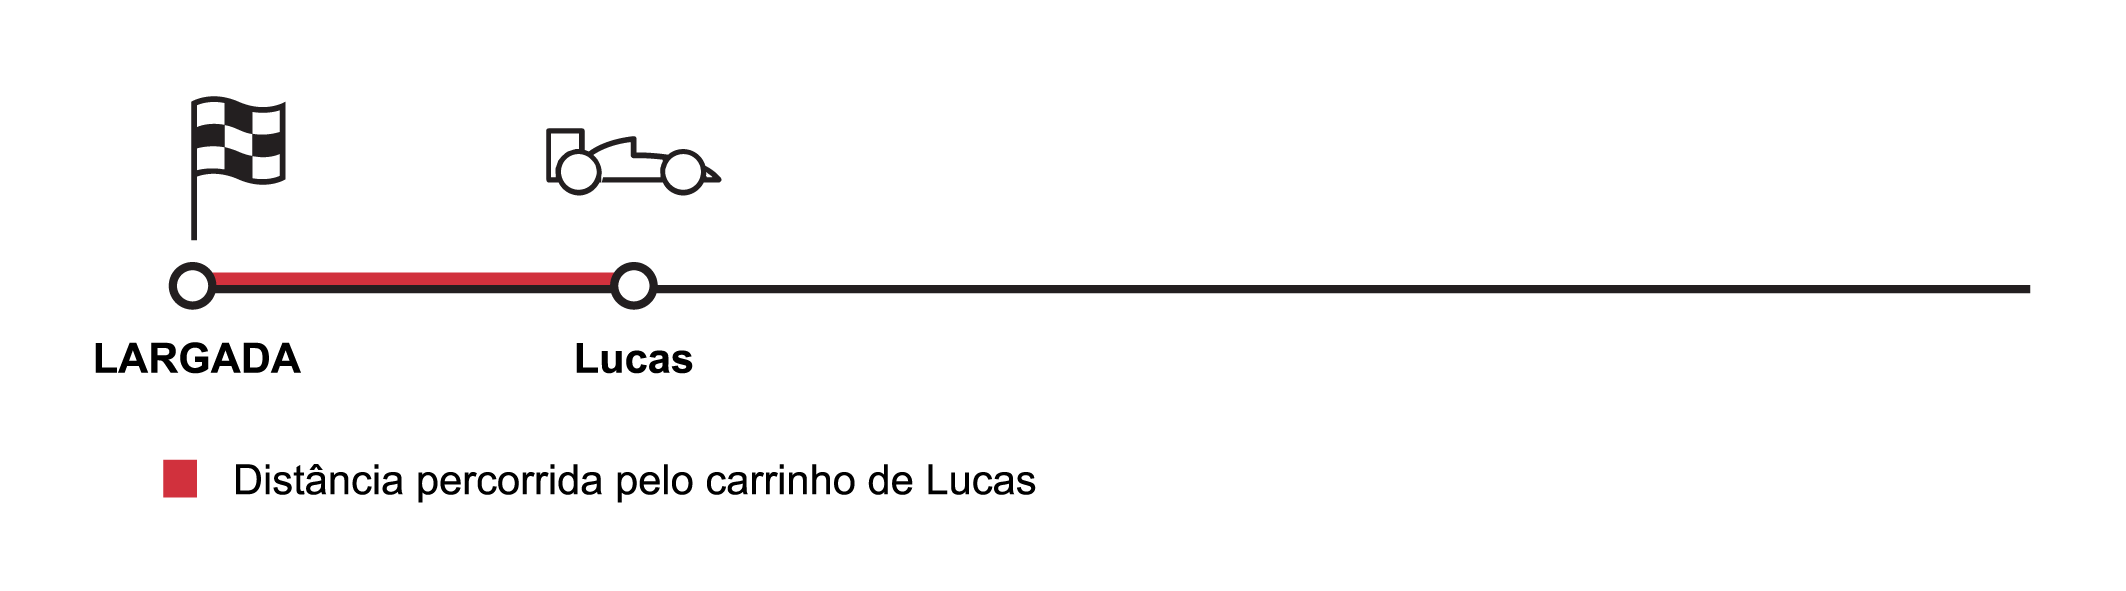
\includegraphics[width=450pt, keepaspectratio]{licao02/ativ12_fig01.png}
\end{center}

Sabe-se que:

\begin{enumerate} [\quad a)] %s
  \item     O carrinho de Matheus só conseguiu ir até a metade da distância percorrida pelo carrinho de Lucas.
  \item     O carrinho de Heitor conseguiu ir até     $\frac{3}{2}$     da distância percorrida pelo carrinho de Lucas.
  \item     O carrinho de Rafael conseguiu ir até     $\frac{4}{2}$     da distância percorrida pelo carrinho de Lucas.
  \item     O carrinho de Enzo conseguiu ir até     $\frac{5}{2}$     da distância percorrida pelo carrinho de Lucas.
  \item     O carrinho de Nicolas conseguiu ir até     $\frac{6}{2}$     da distância percorrida pelo carrinho de Lucas.
  \item     O carrinho de Lorenzo conseguiu ir até     $\frac{6}{4}$     da distância percorrida pelo carrinho de Lucas.
  \item     O carrinho de Guilherme conseguiu ir até o dobro da distância percorrida pelo carrinho de Lucas.
  \item     O carrinho de Samuel conseguiu ir até     $\frac{6}{3}$     da distância percorrida pelo carrinho de Lucas.
\end{enumerate} %s


Com estas informações, marque as posições de parada dos carrinhos de todos os amigos de Lucas no encarte que você irá receber.

\begin{center}
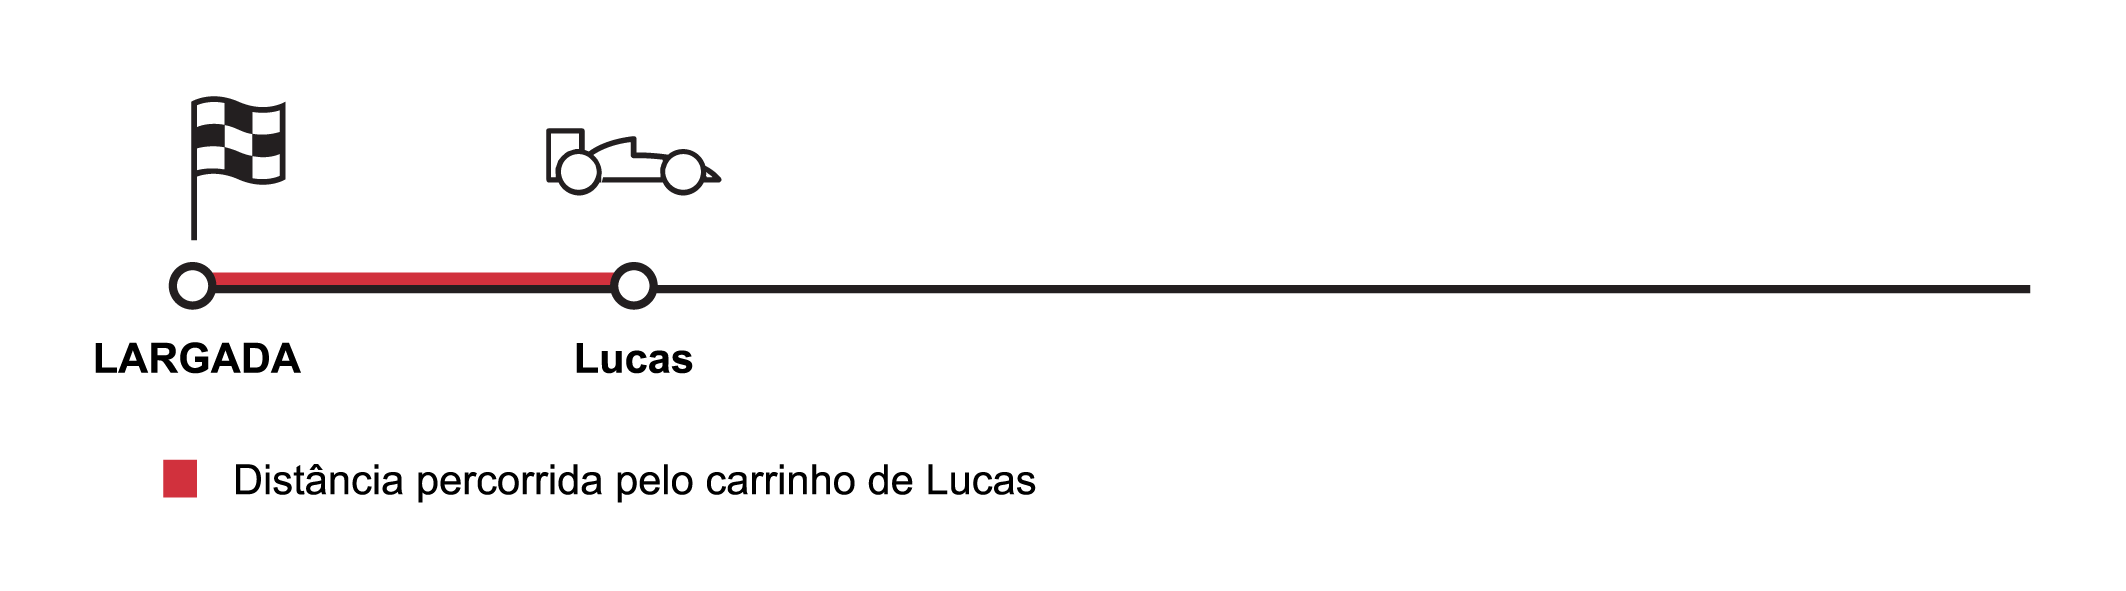
\includegraphics[width=450pt, keepaspectratio]{licao02/ativ12_fig01.png}
\end{center}


Os carrinhos de Rafael e Samuel pararam no mesmo lugar? Explique.


\subsection{Atividade}

Anita, Gustavo e Henrique descobriram que todos tinham levado bolo para o lanche.\newline
Anita falou: ``Mamãe colocou metade do bolo no meu lanche.''\newline
Gustavo falou: ``Eu trouxe um terço do bolo que minha tia fez.''\newline
Henrique falou: ``Eu trouxe apenas um quinto do bolo que minha mãe preparou!''\newline
Para surpresa de todos, ao retirarem seus lanches da mochila, descobriram que todos traziam-no em  embalagens iguais, portanto traziam a mesma quantidade de bolo.\newline
Como você explica tal situação?


\section{QUEBRANDO A CUCA }
\vspace*{-.4cm}


\subsection{Atividade}

(NAEP, 1992) Pense cuidadosamente nesta questão. Escreva uma resposta completa. Você pode usar desenhos, palavras e números para explicar sua resposta. Certifique-se de mostrar todo o seu raciocínio.

José comeu $\frac{1}{2}$ de uma pizza. Ella comeu $\frac{1}{2}$ de uma outra pizza. José disse que ele comeu mais pizza do que Ella, mas Ella diz que eles comeram a mesma quantidade. Use palavras, figuras ou números para mostrar que José pode estar certo.
%\vspace*{-.5cm}


\subsection{Atividade}

Complete as sentenças a seguir com uma fração adequada (use notação simbólica matemática). Perceba que uma mesma região pintada pode ser descrita por frações diferentes, dependendo da unidade considerada.

%definição da região limitada pelos 2 hexágonos encaixados.
\def \tripinha{ (30:4) -- (90:4) -- (150:4)--(210:4)--(270:4)--(330:4) [shift={({4*sqrt(3)},0)}] --(270:4) -- (330:4) -- (30:4) -- (90:4)--(150:4)--cycle;}
%definição da região limitada pelos 3 hexágonos encaixados.
\def \tripa{ (30:4) -- (90:4) -- (150:4)--(210:4)--(270:4)--(330:4) [shift={({4*sqrt(3)},0)}] --(270:4) -- (330:4) [shift={({4*sqrt(3)},0)}]--  (270:4) -- (330:4) -- (30:4) -- (90:4)--(150:4) [shift={({-4*sqrt(3)},0)}] -- (90:4) -- (150:4)--cycle;}

\begin{enumerate} [\quad a)] %s
%a
\item     A região pintada em vermelho em
\begin{tikzpicture}[scale=1.3]
 \draw \tripa;
\begin{scope}
 \clip \tripa;
\draw[fill=attention] (-4,-4) rectangle (0,4);
\draw[fill=common, fill opacity=.3] (0,-4) rectangle (20,4);
\end{scope}
\end{tikzpicture}
é
\begin{tikzpicture} \draw (0,0)--(20,0);\end{tikzpicture}
de
\begin{tikzpicture}[scale=1.3]
\draw[fill=common, fill opacity=.3] (30:4) -- (90:4) -- (150:4) -- (210:4) -- (270:4) -- (330:4)--cycle;
\end{tikzpicture}.
 %b
\item     A região pintada em vermelho em
\begin{tikzpicture}[scale=1.3]
 \draw \tripa;
\begin{scope}
 \clip \tripa;
\draw[fill=attention] (-4,-4) rectangle (0,4);
\draw[fill=common, fill opacity=.3] (0,-4) rectangle (20,4);
\end{scope}
\end{tikzpicture}
é
\begin{tikzpicture} \draw (0,0)--(20,0);\end{tikzpicture}
de
\begin{tikzpicture}[scale=1.3]
 \draw[fill=common, fill opacity=.3] (30:4) -- (90:4) -- (150:4)--(210:4)--(270:4)--(330:4) [shift={({4*sqrt(3)},0)}] --(270:4) -- (330:4) --(30:4) -- (90:4) -- (150:4)--cycle;
\end{tikzpicture}.

%c
\item     A região pintada em vermelho em \begin{tikzpicture}[scale=1.3]
 \draw \tripa;
\begin{scope}
 \clip \tripa;
\draw[fill=attention] (-4,-4) rectangle (0,4);
\draw[fill=common, fill opacity=.3] (0,-4) rectangle (20,4);
\end{scope}
\end{tikzpicture}
     é \begin{tikzpicture} \draw (0,0)--(20,0);\end{tikzpicture}    de
\begin{tikzpicture}[scale=1.3]
\draw[fill=common, fill opacity=.3] \tripa;
\end{tikzpicture}.

%d
 \item     A região pintada em vermelho em  \begin{tikzpicture}[scale=1.3]
 \draw \tripa;
\begin{scope}
 \clip \tripa;
\draw[fill=attention] (-4,-4) rectangle ({4*sqrt(3)},4);
\draw[fill=common, fill opacity=.3] ({4*sqrt(3)},-4) rectangle ({10*sqrt(3)},4);
\end{scope}
\end{tikzpicture}  é \begin{tikzpicture} \draw (0,0)--(20,0);\end{tikzpicture}    de
\begin{tikzpicture}[scale=1.3]
\draw[fill=common, fill opacity=.3] (30:4) -- (90:4) -- (150:4) -- (210:4) -- (270:4) -- (330:4)--cycle;
\end{tikzpicture}.
%e
\item     A região pintada em vermelho em   \begin{tikzpicture}[scale=1.3]
 \draw \tripa;
\begin{scope}
 \clip \tripa;
\draw[fill=attention] (-4,-4) rectangle ({4*sqrt(3)},4);
\draw[fill=common, fill opacity=.3] ({4*sqrt(3)},-4) rectangle ({10*sqrt(3)},4);
\end{scope}
\end{tikzpicture}    é \begin{tikzpicture} \draw (0,0)--(20,0);\end{tikzpicture}    de
\begin{tikzpicture}[scale=1.3]
 \draw[fill=common, fill opacity=.3] (30:4) -- (90:4) -- (150:4)--(210:4)--(270:4)--(330:4) [shift={({4*sqrt(3)},0)}] --(270:4) -- (330:4) --(30:4) -- (90:4) -- (150:4)--cycle;
\end{tikzpicture}.

%f
\item     A região pintada em vermelho em  \begin{tikzpicture}[scale=1.3]
 \draw \tripa;
\begin{scope}
 \clip \tripa;
\draw[fill=attention] (-4,-4) rectangle ({4*sqrt(3)},4);
\draw[fill=common, fill opacity=.3] ({4*sqrt(3)},-4) rectangle ({10*sqrt(3)},4);
\end{scope}
\end{tikzpicture}   é \begin{tikzpicture} \draw (0,0)--(20,0);\end{tikzpicture}    de
\begin{tikzpicture}[scale=1.3]
\draw[fill=common, fill opacity=.3] \tripa;
\end{tikzpicture}.

%g
\item     A região pintada em vermelho em
\begin{tikzpicture}[scale=1.3]
 \draw \tripa;
\begin{scope}
 \clip \tripa;
\draw[fill=attention] (-4,-4) rectangle ({8*sqrt(3)},4);
\draw[fill=common, fill opacity=.3] ({8*sqrt(3)},-4) rectangle ({10*sqrt(3)},4);
\end{scope}
\end{tikzpicture}
é \begin{tikzpicture} \draw (0,0)--(20,0);\end{tikzpicture}    de
\begin{tikzpicture}[scale=1.3]
\draw[fill=common, fill opacity=.3] (30:4) -- (90:4) -- (150:4) -- (210:4) -- (270:4) -- (330:4)--cycle;
\end{tikzpicture}.
%h
\item     A região pintada em vermelho em  \begin{tikzpicture}[scale=1.3]
 \draw \tripa;
\begin{scope}
 \clip \tripa;
\draw[fill=attention] (-4,-4) rectangle ({8*sqrt(3)},4);
\draw[fill=common, fill opacity=.3] ({8*sqrt(3)},-4) rectangle ({10*sqrt(3)},4);
\end{scope}
\end{tikzpicture} é \begin{tikzpicture} \draw (0,0)--(20,0);\end{tikzpicture}    de
\begin{tikzpicture}[scale=1.3]
 \draw[fill=common, fill opacity=.3] (30:4) -- (90:4) -- (150:4)--(210:4)--(270:4)--(330:4) [shift={({4*sqrt(3)},0)}] --(270:4) -- (330:4) --(30:4) -- (90:4) -- (150:4)--cycle;
\end{tikzpicture}.

%i
\item     A região pintada em vermelho em
\begin{tikzpicture}[scale=1.3]
 \draw \tripa;
\begin{scope}
 \clip \tripa;
\draw[fill=attention] (-4,-4) rectangle ({8*sqrt(3)},4);
\draw[fill=common, fill opacity=.3] ({8*sqrt(3)},-4) rectangle ({10*sqrt(3)},4);
\end{scope}
\end{tikzpicture}
é \begin{tikzpicture} \draw (0,0)--(20,0);\end{tikzpicture}    de
\begin{tikzpicture}[scale=1.3]
\draw[fill=common, fill opacity=.3] \tripa;
\end{tikzpicture}.
%j
\item     A região pintada em vermelho em
  \begin{tikzpicture}[scale=1.3]
 \draw \tripa;
\begin{scope}
 \clip \tripa;
\draw[fill=attention] (-4,-4) rectangle ({12*sqrt(3)},4);
\end{scope}
\end{tikzpicture}
é \begin{tikzpicture} \draw (0,0)--(20,0);\end{tikzpicture}    de
\begin{tikzpicture}[scale=1.3]
\draw[fill=common, fill opacity=.3] (30:4) -- (90:4) -- (150:4) -- (210:4) -- (270:4) -- (330:4)--cycle;
\end{tikzpicture}.
%k
\item     A região pintada em vermelho em
\begin{tikzpicture}[scale=1.3]
 \draw \tripa;
\begin{scope}
 \clip \tripa;
\draw[fill=attention] (-4,-4) rectangle ({12*sqrt(3)},4);
\end{scope}
\end{tikzpicture}
é \begin{tikzpicture} \draw (0,0)--(20,0);\end{tikzpicture}    de
\begin{tikzpicture}[scale=1.3]
 \draw[fill=common, fill opacity=.3] (30:4) -- (90:4) -- (150:4)--(210:4)--(270:4)--(330:4) [shift={({4*sqrt(3)},0)}] --(270:4) -- (330:4) --(30:4) -- (90:4) -- (150:4)--cycle;
\end{tikzpicture}.

%l
\item     A região pintada em vermelho em
  \begin{tikzpicture}[scale=1.3]
 \draw \tripa;
\begin{scope}
 \clip \tripa;
\draw[fill=attention] (-4,-4) rectangle ({12*sqrt(3)},4);
\end{scope}
\end{tikzpicture}
é \begin{tikzpicture} \draw (0,0)--(20,0);\end{tikzpicture}    de
\begin{tikzpicture}[scale=1.3]
\draw[fill=common, fill opacity=.3] \tripa;
\end{tikzpicture}.

\end{enumerate} %s


\subsection{Atividade}

Miguel disse para Alice que a parte pintada de vermelho na figura a seguir corresponde a $\frac{3}{5}$ da figura, pois ela está dividida em 5 partes e 3 partes estão pintadas. Você concorda com a afirmação e com a justificativa de Miguel? Explique!

\begin{center}
\begin{tikzpicture}[scale=1.5]
%\fill[fill=attention,fill opacity=0.1] (0.,5.) -- (9.,5.) -- (9.,-5.) -- (0.,-5.) -- cycle;
\fill[fill=attention,fill opacity=1.0] (0.,5.) -- (0.,0.) -- (9.,0.) -- (9.,5.) -- cycle;
\fill[common, fill opacity=.3] (0,-5) rectangle (9,0);
\draw   (0.,5.)-- (9.,5.);
\draw   (9.,5.)-- (9.,-5.);
\draw   (9.,-5.)-- (0.,-5.);
\draw   (0.,-5.)-- (0.,5.);
\draw   (0.,5.)-- (0.,0.);
\draw   (0.,0.)-- (9.,0.);
\draw   (9.,0.)-- (9.,5.);
\draw   (9.,5.)-- (0.,5.);
\draw   (0.,5.)-- (9.,5.);
\draw   (9.,0.)-- (0.,0.);
\draw   (0.,0.)-- (0.,5.);
\draw   (9.,5.)-- (9.,0.);
\draw   (3.,0.)-- (3.,5.);
\draw   (6.,5.)-- (6.,0.);
\draw   (4.5,-5.)-- (4.5,0.);
\draw   (0.,-5.)-- (9.,-5.);
\draw   (9.,-5.)-- (9.,0.);
\draw   (9.,0.)-- (0.,0.);
\draw   (0.,0.)-- (0.,-5.);
% \begin{scriptsize}
% %\draw[color=ffqqqq] (4.725943121127749,2.6736730506884316) node {$pol2$};
% \end{scriptsize}
\end{tikzpicture}
\end{center}
\vspace*{-.6cm}

\subsection{Atividade}

A figura a seguir tem 3 partes pintadas de vermelho e 4 partes pintadas de branco. É correto afirmar que a parte pintada de vermelho corresponde a $\frac{3}{4}$ da figura? Explique.
\begin{center}
\begin{tikzpicture}[scale=3.5]%[line cap=round,line join=round,>=triangle 45,x=1.0cm,y=1.0cm]
\fill[fill=attention] (0.,3.) -- (3.,3.) -- (3.,0.) -- (0.,0.) -- cycle;
\fill[common, fill opacity=.3] (3,0) rectangle (7,3);
\draw (1.,3.)-- (1.,0.);
\draw (2.,0.)-- (2.,3.);
\draw (3.,3.)-- (3.,0.);
\draw (4.,0.)-- (4.,3.);
\draw (5.,3.)-- (5.,0.);
\draw (6.,0.)-- (6.,3.);
\draw (7.,3.)-- (7.,0.);
\draw (0.,3.)-- (7.,3.);
\draw (7.,3.)-- (7.,0.);
\draw (7.,0.)-- (0.,0.);
\draw (0.,0.)-- (0.,3.);
\end{tikzpicture}
\end{center}

\subsection{Atividade}

\begin{enumerate} [\quad a)] %s
  \item     A região em vermelho na figura a seguir representa $\frac{1}{2}$ ou $\frac{1}{4}$?
\begin{center}
\begin{tikzpicture}[scale=1.5]
 \draw \tripinha;
\begin{scope}
 \clip \tripinha;
\draw[fill=attention] (-4,-4) rectangle (0,4);
\draw[fill=common, fill opacity=.3] (0,-4) rectangle (12,4);
\end{scope}
\end{tikzpicture}
\end{center}

  \item     A região em vermelho na figura a seguir representa     $\frac{1}{2}$     ou     $\frac{3}{2}$?
\begin{center}
\begin{tikzpicture}[scale=1.5]
 \draw \tripa;
\begin{scope}
 \clip \tripa;
\draw[fill=attention] (-4,-4) rectangle ({4*sqrt(3)},4);
\draw[fill=common, fill opacity=.3] ({4*sqrt(3)},-4) rectangle ({12*sqrt(3)},4);
\end{scope}
\end{tikzpicture}
\end{center}
\def \tripalonga{ (30:4) -- (90:4) -- (150:4)--(210:4)--(270:4)--(330:4) [shift={({4*sqrt(3)},0)}] --(270:4) -- (330:4) [shift={({4*sqrt(3)},0)}] --(270:4) -- (330:4)[shift={({4*sqrt(3)},0)}] --(270:4) -- (330:4) [shift={({4*sqrt(3)},0)}]--  (270:4) -- (330:4) -- (30:4) -- (90:4)--(150:4) [shift={({-4*sqrt(3)},0)}] -- (90:4) -- (150:4)[shift={({-4*sqrt(3)},0)}] -- (90:4) -- (150:4) [shift={({-4*sqrt(3)},0)}] -- (90:4) -- (150:4)--cycle;}

  \item     A região em vermelho na figura a seguir representa     $\frac{3}{5}$     ou     $3$?
\begin{center}
\begin{tikzpicture}[scale=1.5]
 \draw \tripalonga;
\begin{scope}
 \clip \tripalonga;
  \draw[fill=attention] (-4,-4) rectangle ({10*sqrt(3)},4);
\draw[fill=common, fill opacity=.3] ({10*sqrt(3)},-4) rectangle ({20*sqrt(3)},4);
\end{scope}
\end{tikzpicture}
\end{center}

  \end{enumerate} %s


\subsection{Atividade}

Júlia, Davi e Laura estavam estudando a figura a seguir.
\begin{center}
\begin{tikzpicture}[scale=4]
%\fill(1.,3.) -- (6.,3.) -- (6.,0.02) -- (1.,0.) -- cycle;
\fill[attention] (1.,3.) -- (4.,3.) -- (4.,0.012) -- (1.,0.) -- cycle;
\fill[common, fill opacity=.3] (4,0) rectangle (6,3);
%\fill[line width=0.pt,color=black,fill=black,fill opacity=1.0] (4.,3.) -- (4.,0.012) -- (6.,0.04) -- (6.,3.) -- cycle;
\draw (1.,3.)-- (1.,0.);
\draw (2.,0.)-- (2.,3.);
\draw (3.,3.)-- (3.,0.);
\draw (4.,0.)-- (4.,3.);
\draw (5.,3.)-- (5.,0.);
\draw (6.,0.)-- (6.,3.);
\draw (1.,3.)-- (6.,3.);
\draw (6.,3.)-- (6.,0.02);
\draw (6.,0.02)-- (1.,0.);
\draw (1.,0.)-- (1.,3.);
\end{tikzpicture}
\end{center}
Júlia disse: ``A parte em vermelho representa $\frac{3}{5}$''. Davi retrucou: ``Não, não! A parte em vermelho representa $\frac{3}{2}$!''. Laura, então acrescentou: ``Eu acho que a parte em vermelho representa $3$!''. Quem está certo? Júlia, Davi ou Laura? Explique!

\subsection{Atividade}

Em uma pizzaria rodízio, 7 amigos comem, ao todo, 38 fatias.

\begin{center}

\includegraphics[width=300pt, keepaspectratio]{licao02/ativ18_fig01.png}
\end{center}


Sabendo que nessa pizzaria cada pizza é repartida em 8 fatias de mesmo tamanho, pergunta-se:
\begin{enumerate} [\quad a)] %s
  \item     Quantas pizzas inteiras comeraram os 7 amigos?
  \item     Que fração de uma pizza comeram  ao todo os amigos?
  \item     É possível que todos os amigos tenham comido o mesmo número de fatias de pizza? Explique.
\end{enumerate} %s

		  
		  
		  
		  
		  
		  
\mbox{}
\thispagestyle{empty}
\newpage

\setcounter{chapter}{2}
\chapter{Frações na reta numérica }
\setcounter{subsection}{0}
\section{EXPLORANDO O ASSUNTO }

\subsection{Atividade}

Os quadrinhos a seguir mostram uma caixa-d'água sendo enchida. 
Para saber que fração da capacidade da caixa-d'água já está com água, será usada uma faixa graduada para indicar o nível de água na caixa. 


  \begin{center}
  \begin{tabular}{cc}
  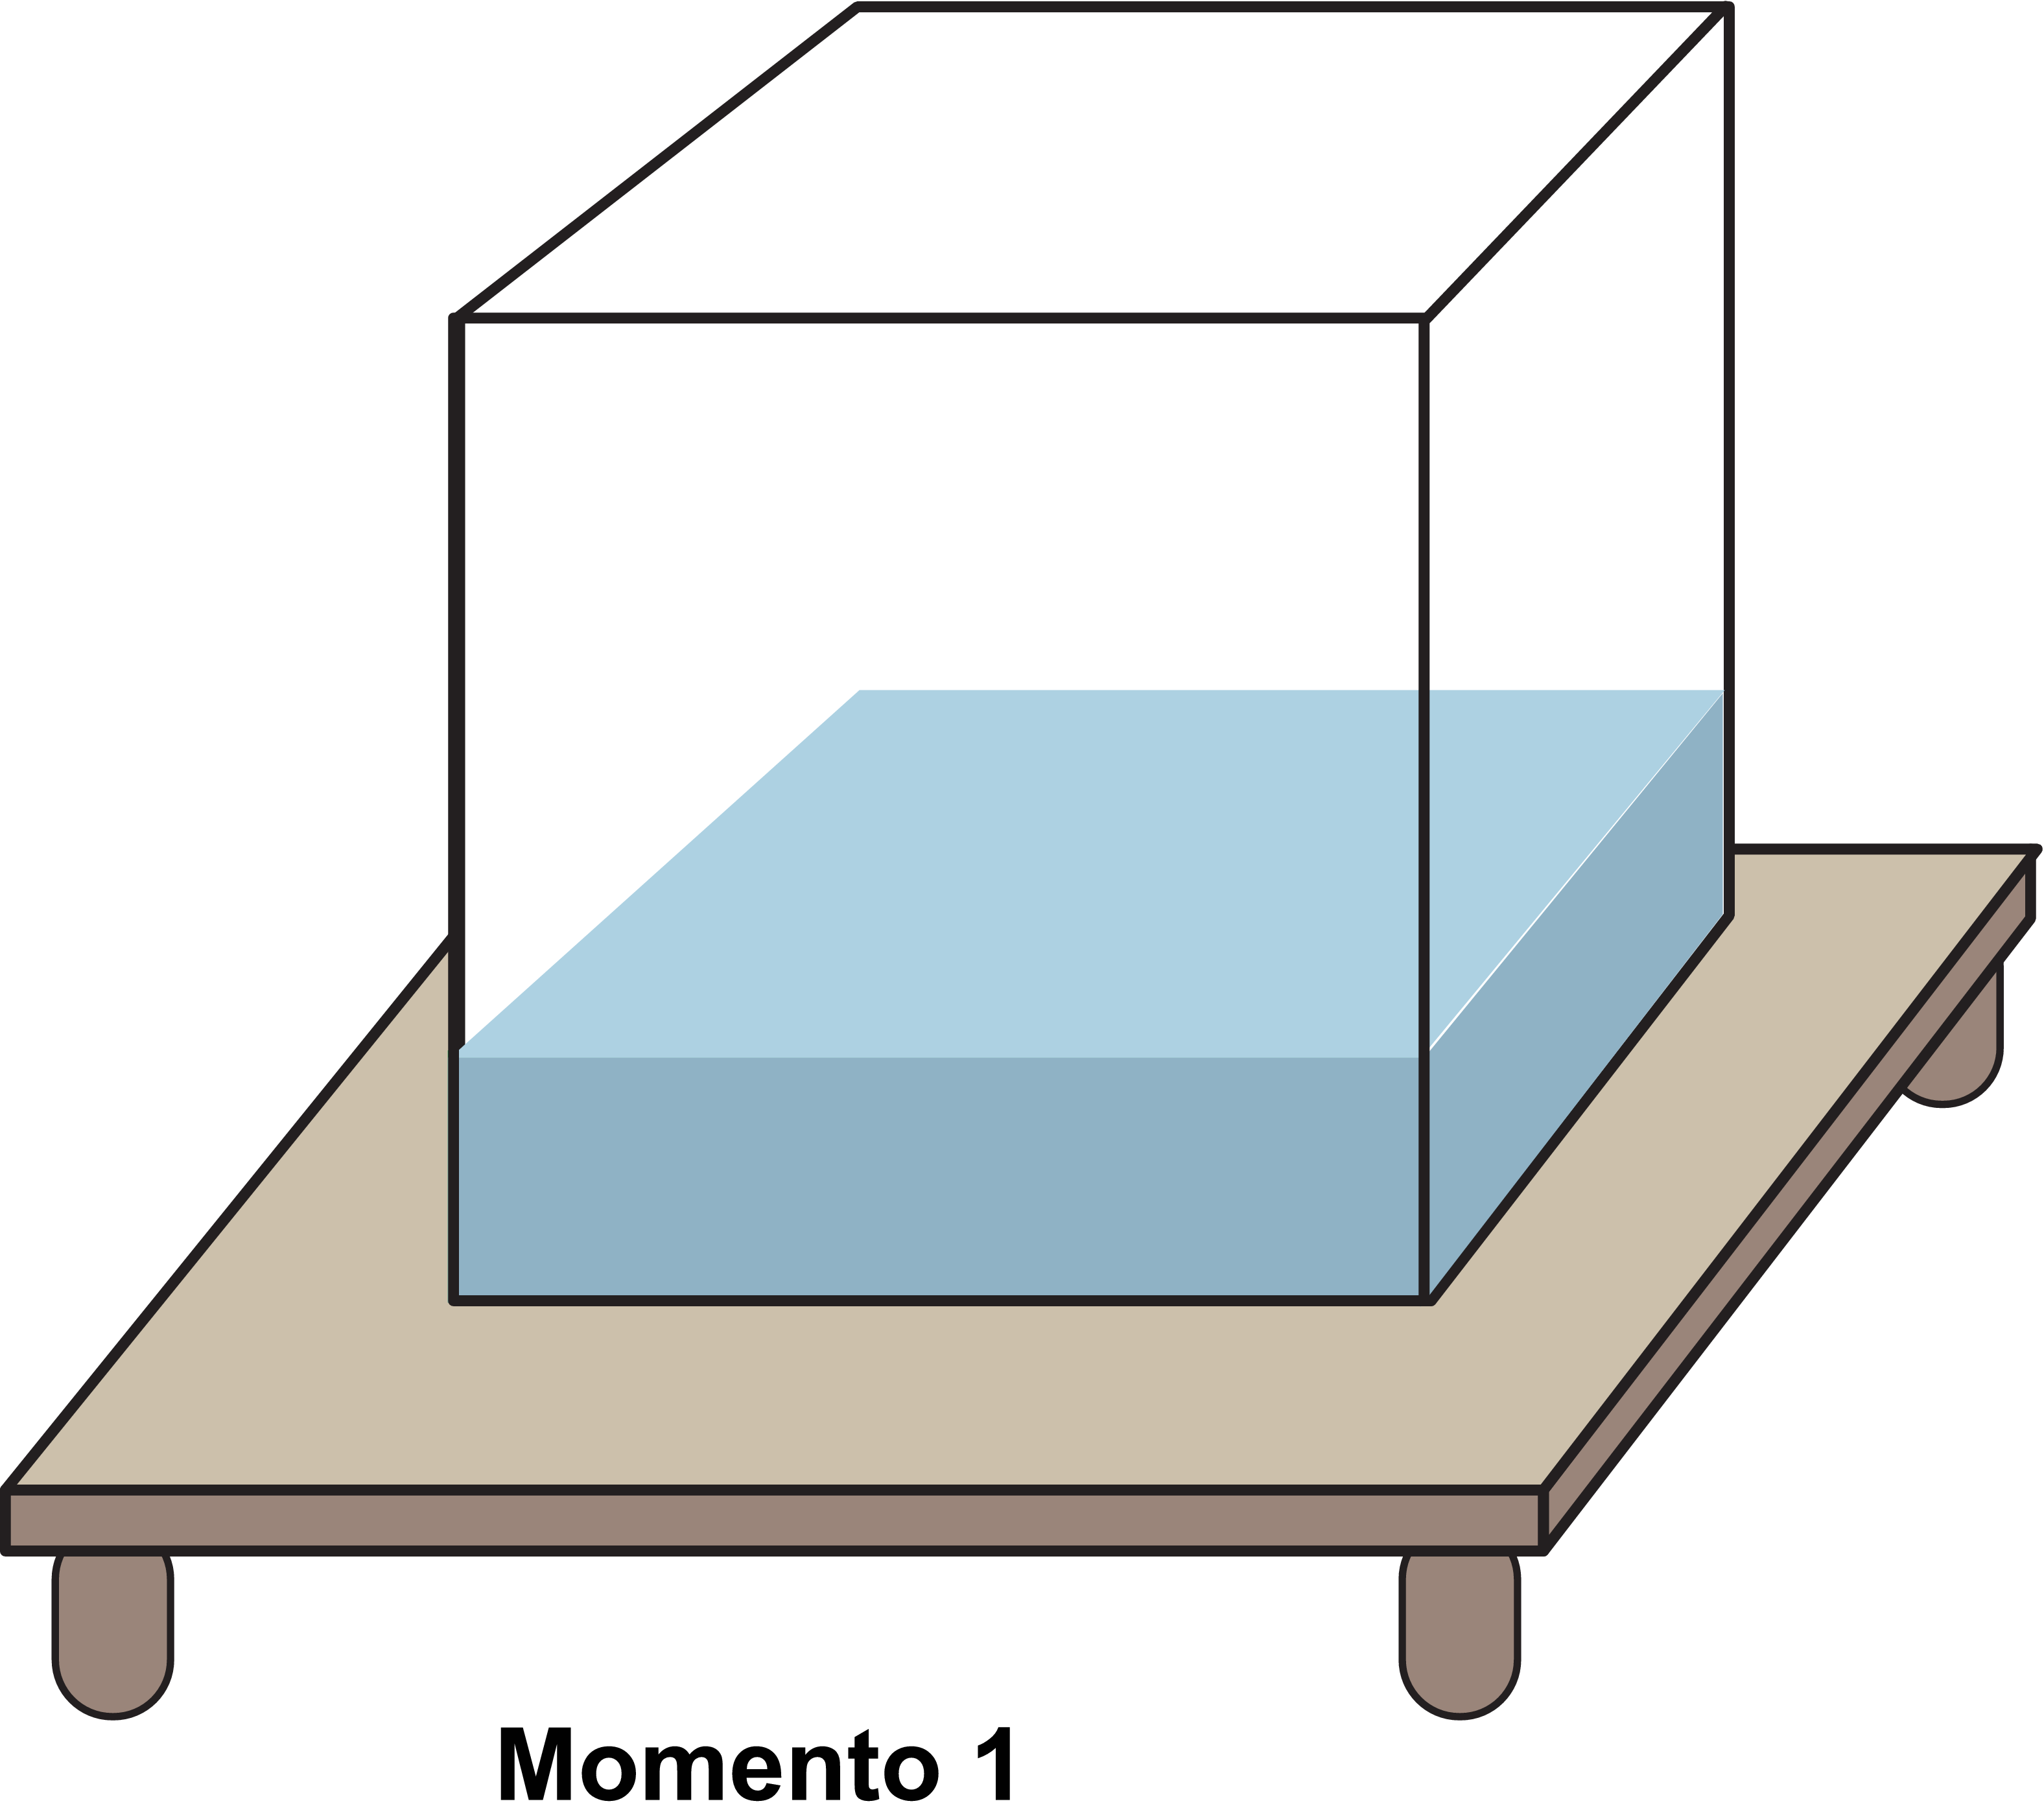
\includegraphics[width=145pt, keepaspectratio]{..//media/cap3/secoes/png/ativ1_fig01.png}  & 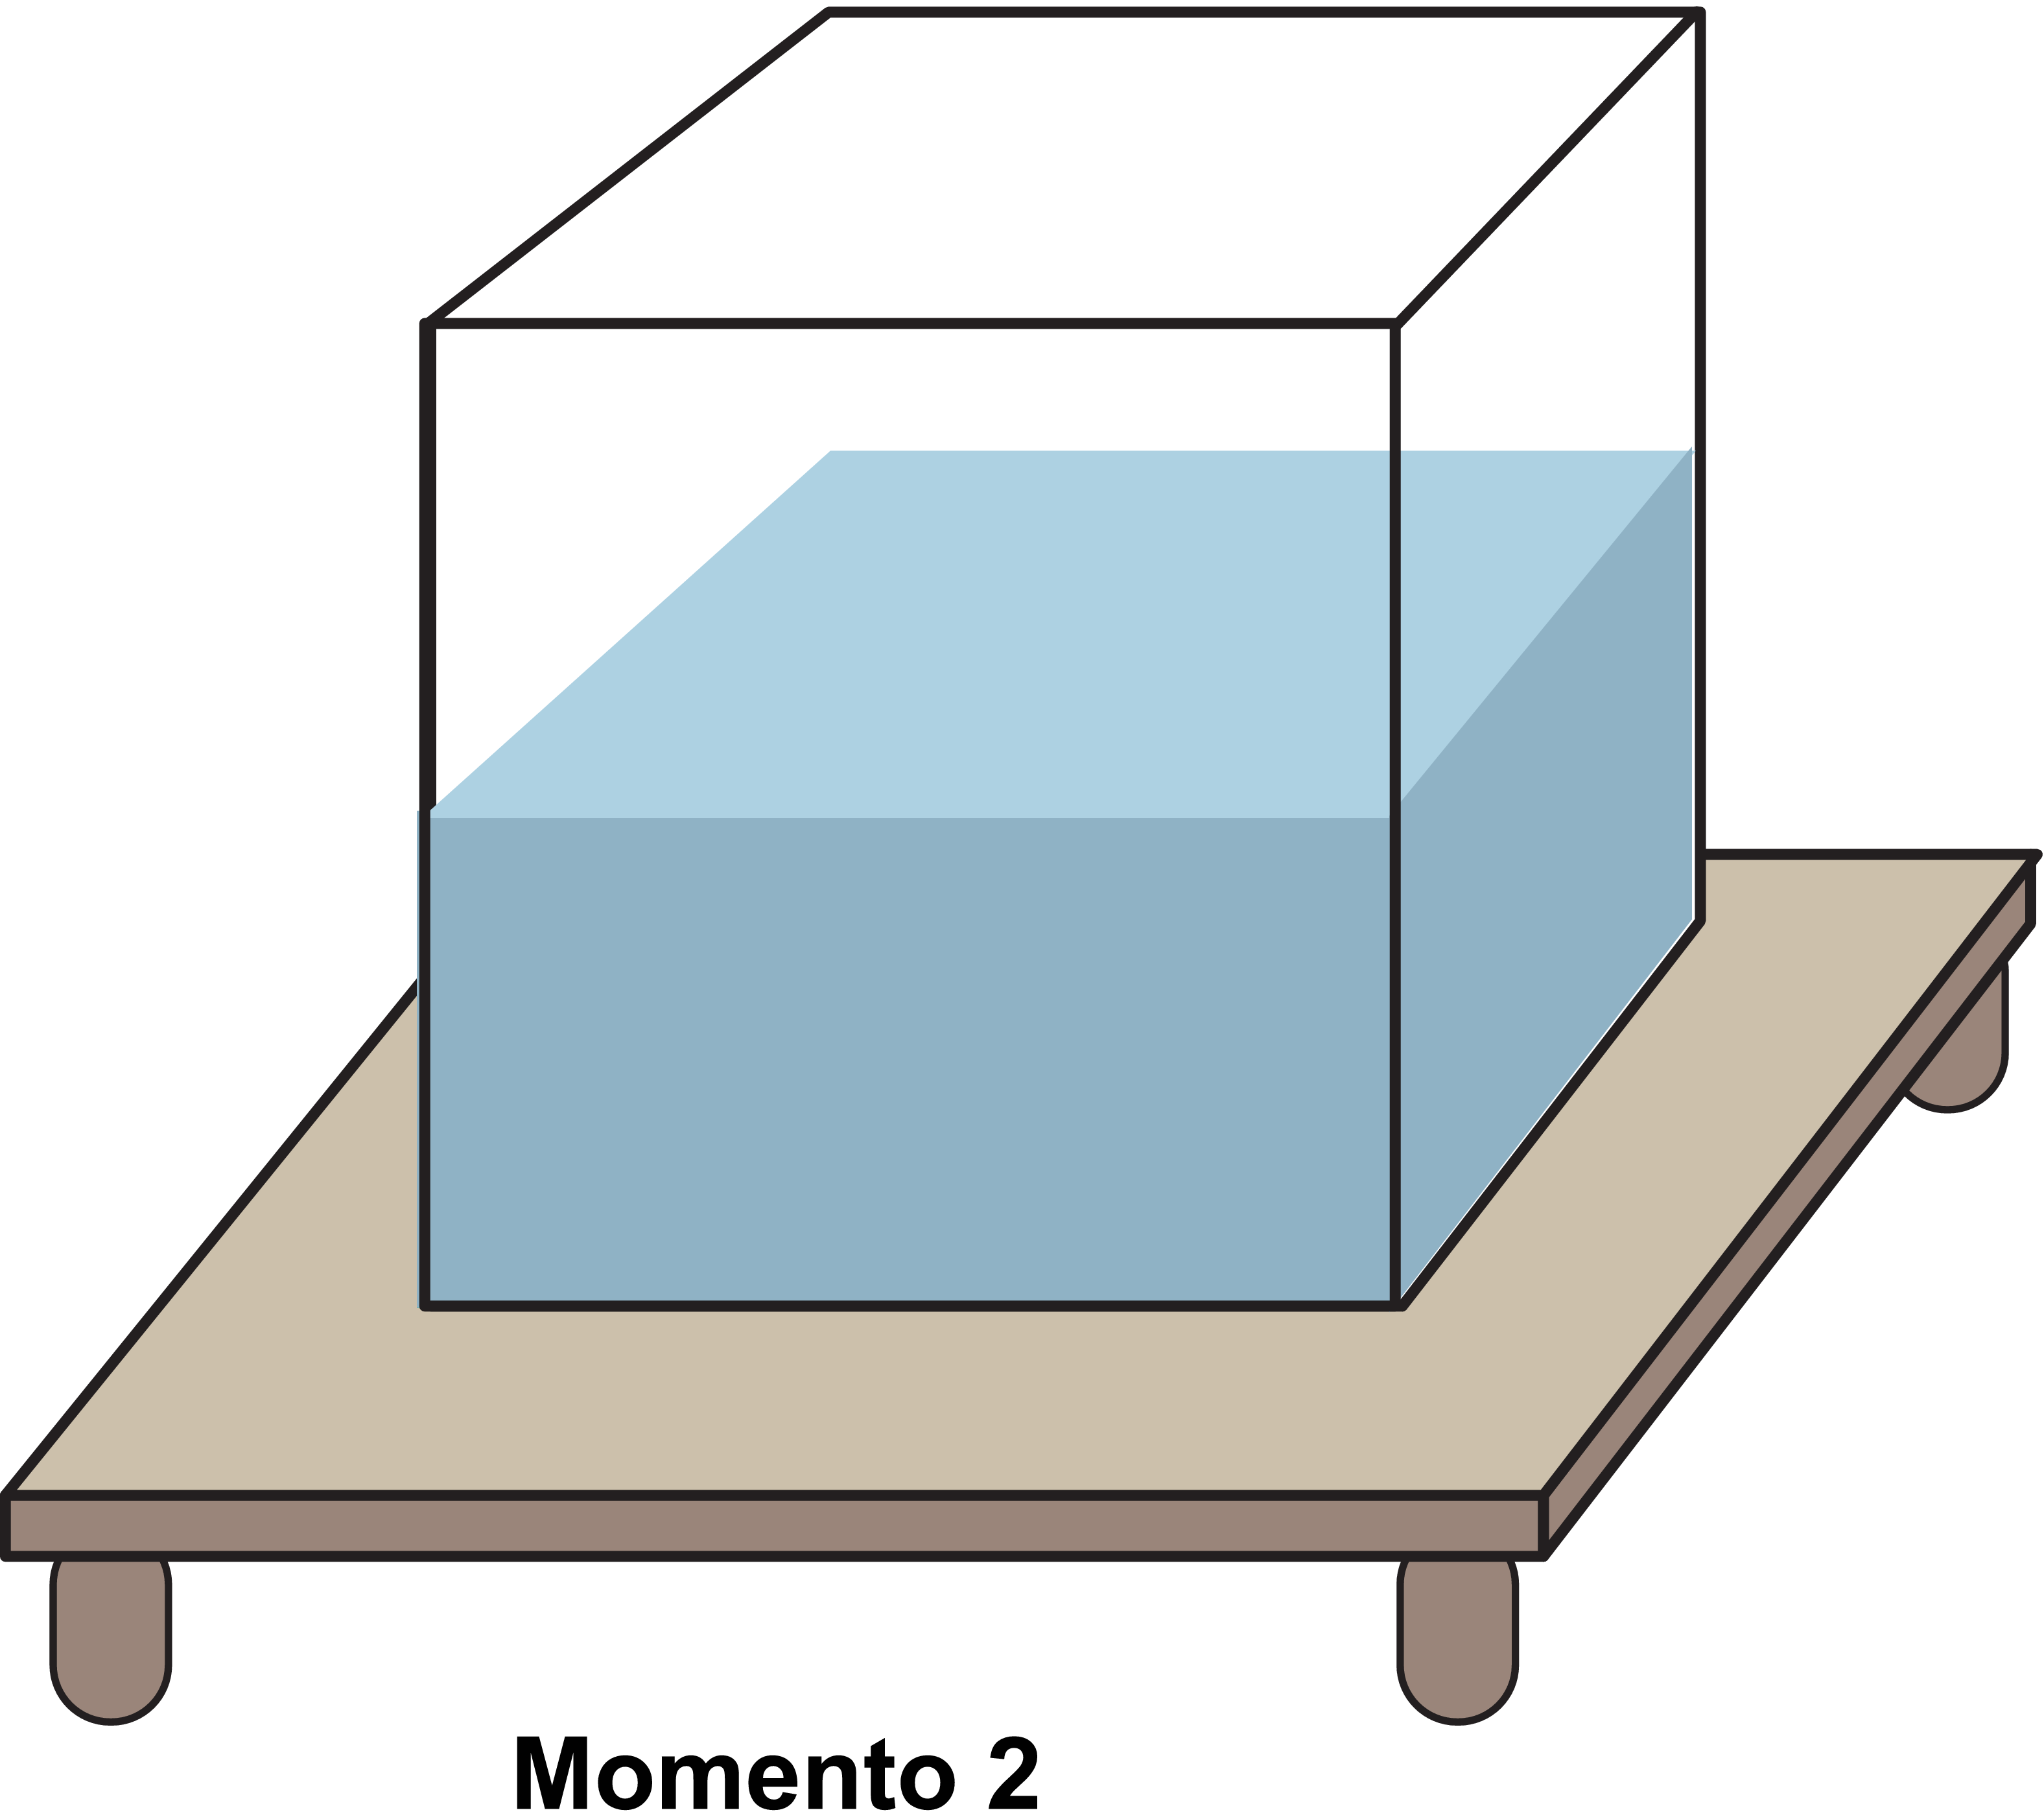
\includegraphics[width=145pt, keepaspectratio]{..//media/cap3/secoes/png/ativ1_fig02.png}
  \end{tabular}\newline
  \begin{tabular}{cc}
  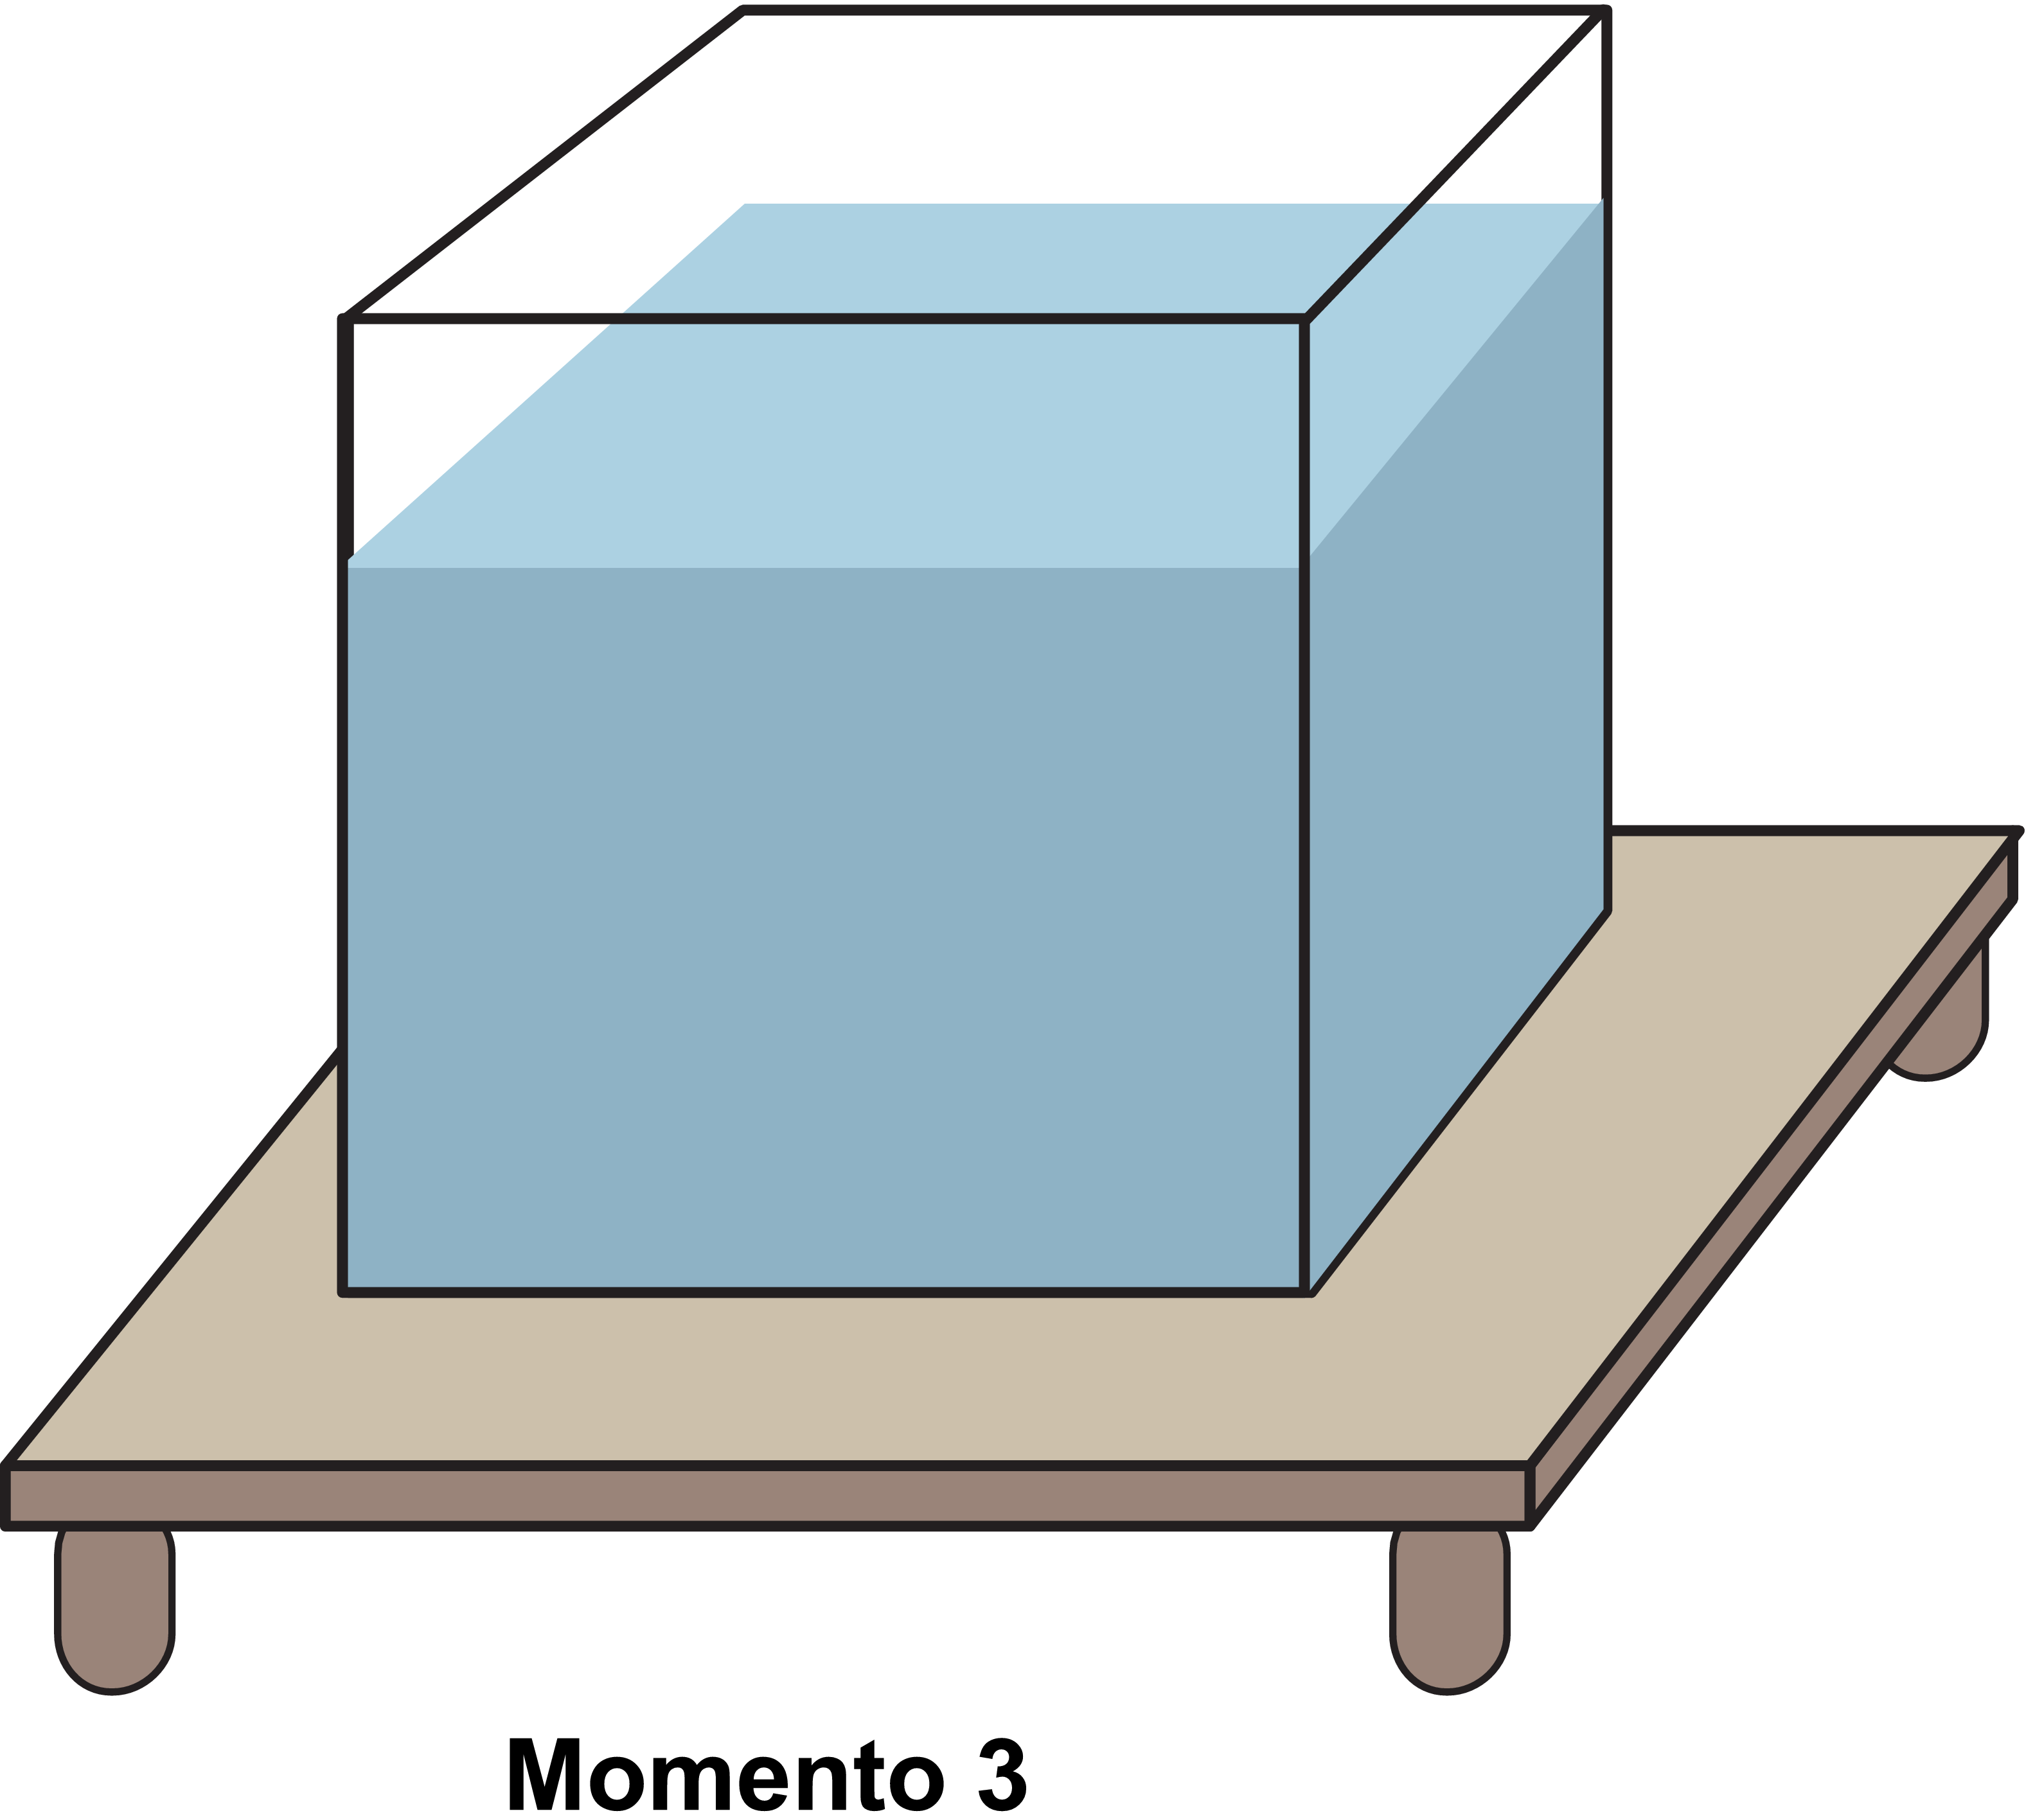
\includegraphics[width=145pt, keepaspectratio]{..//media/cap3/secoes/png/ativ1_fig03.png}  & 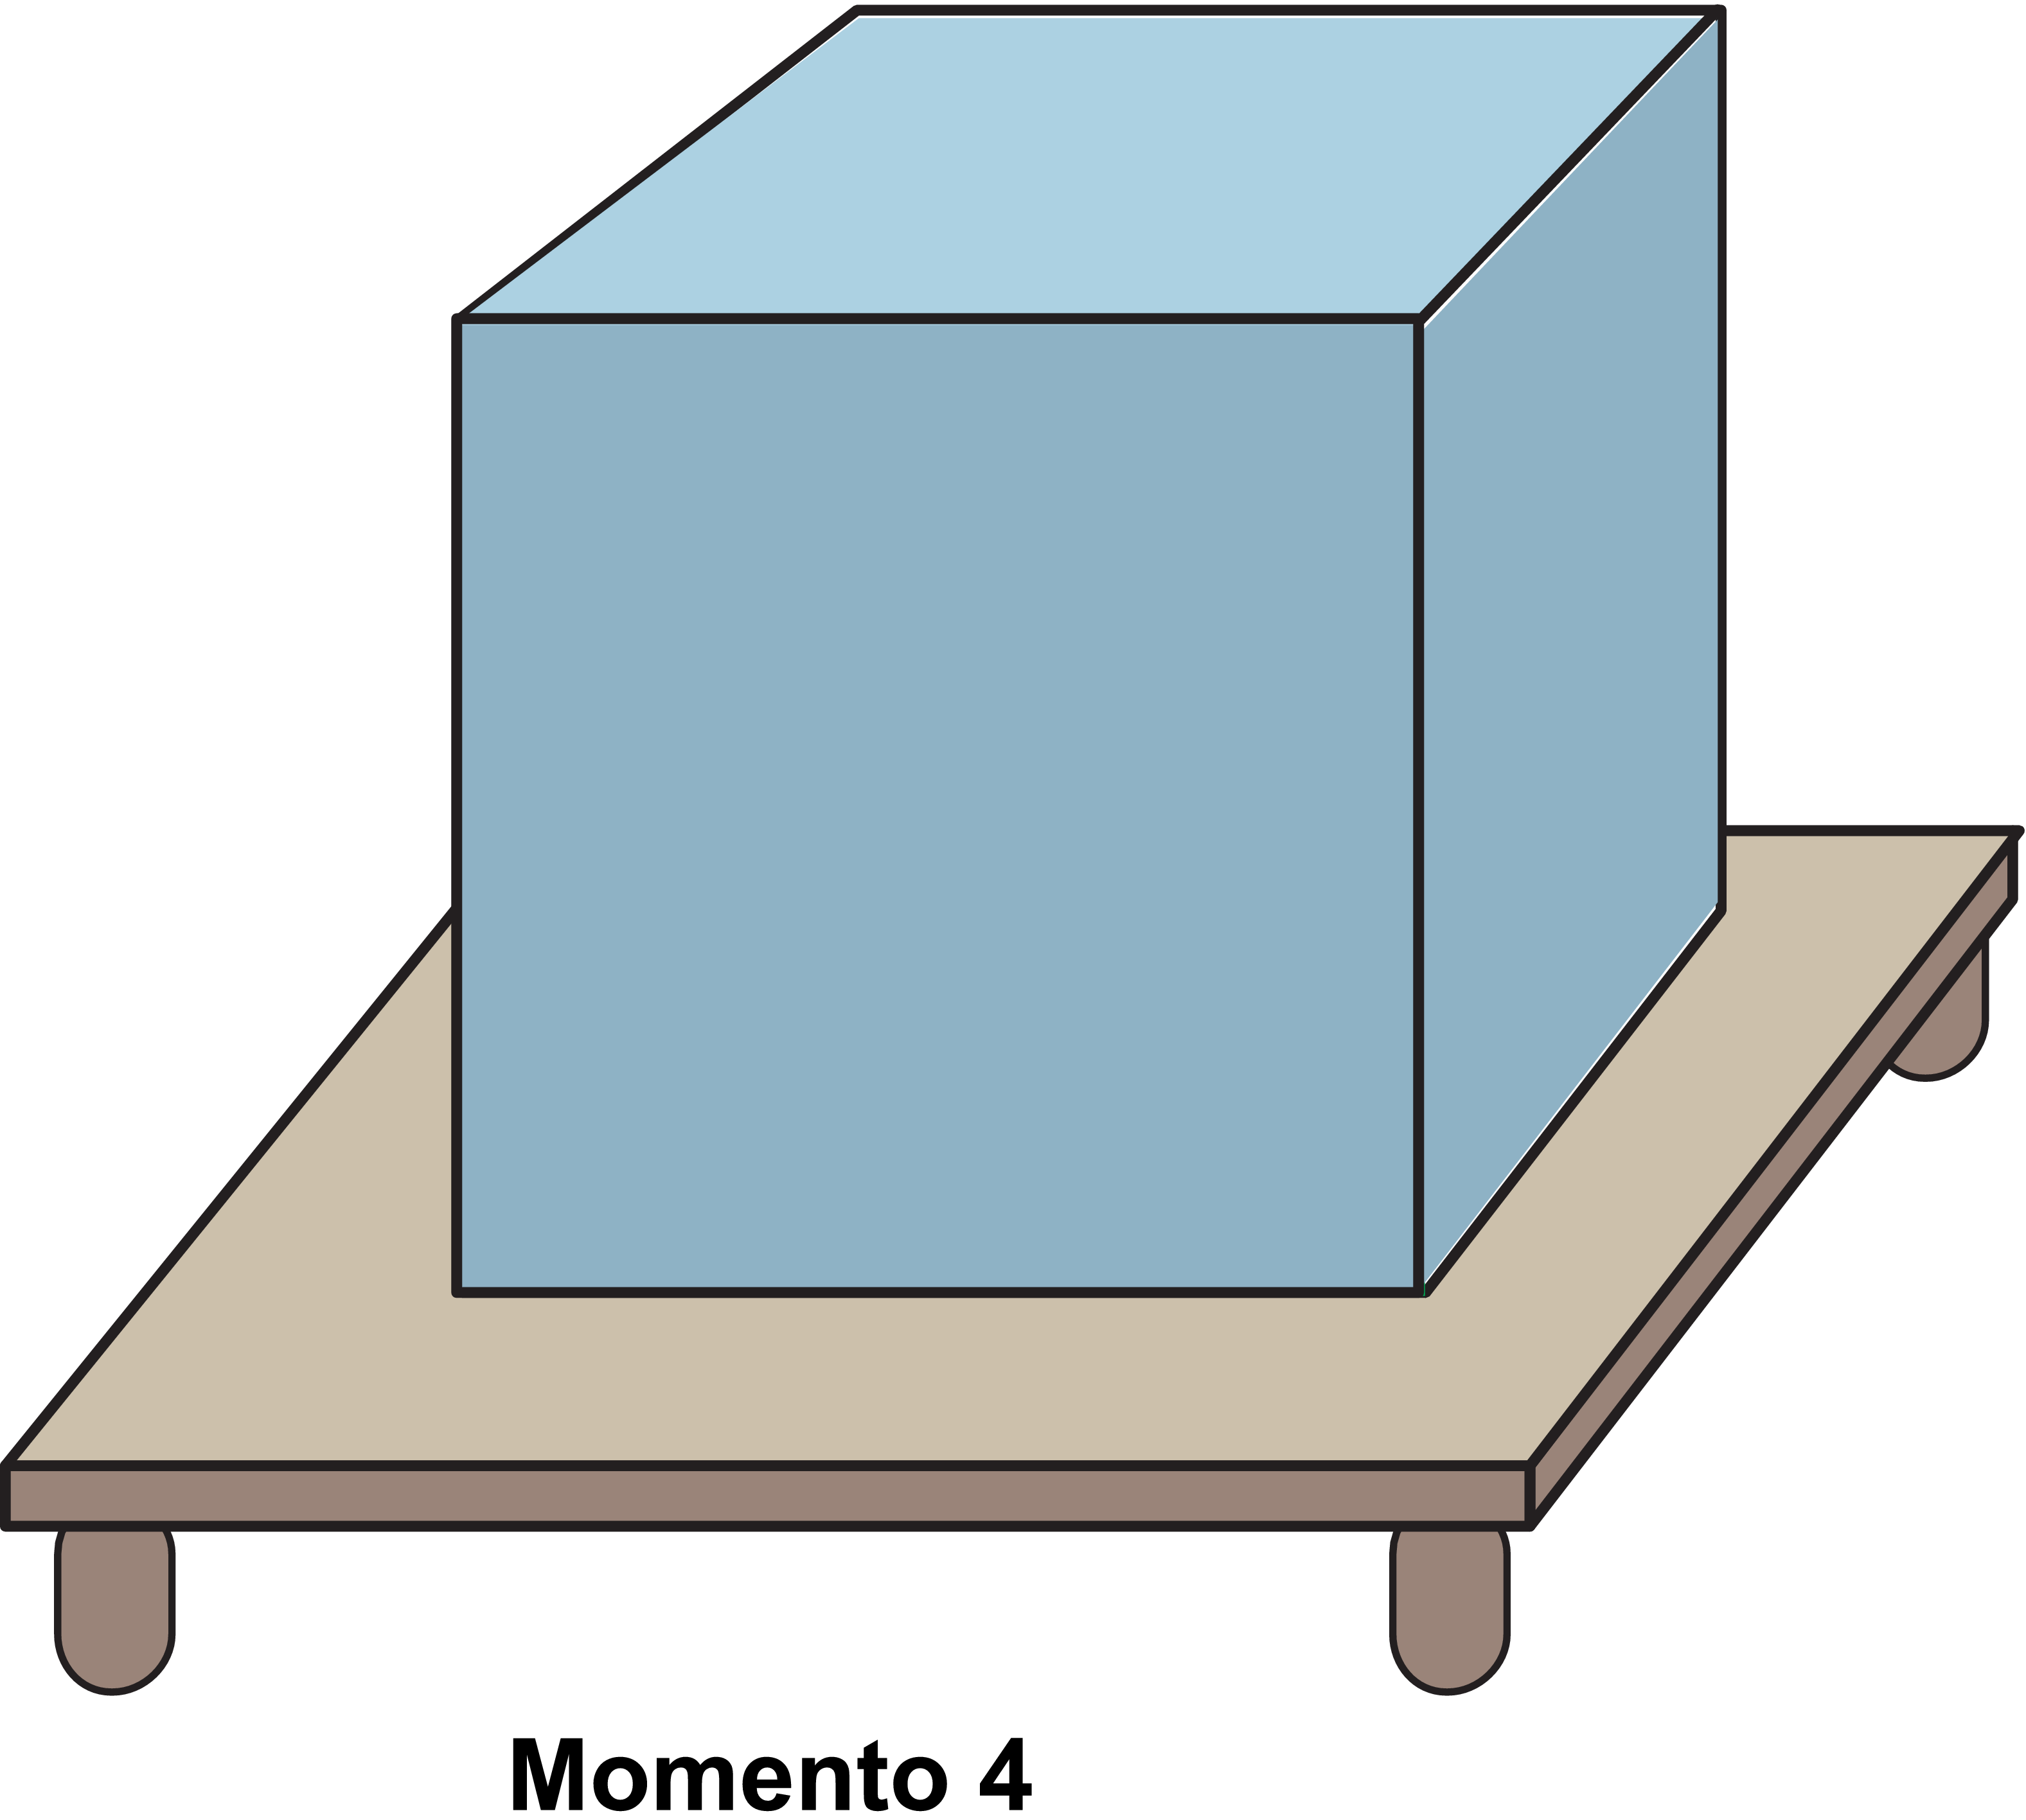
\includegraphics[width=145pt, keepaspectratio]{..//media/cap3/secoes/png/ativ1_fig04.png}
  \end{tabular}
  \end{center}

Escolha, para cada um dos momentos, a graduação que lhe parece mais adequada para registrar a quantidade de agua representada em cada uma das imagens. Explique sua escolha.

  
     \begin{center}
     \begin{tabular}{m{.3\textwidth}m{.3\textwidth}m{.3\textwidth}}
 \parbox[b][.3cm][t]{.3cm}{a)}  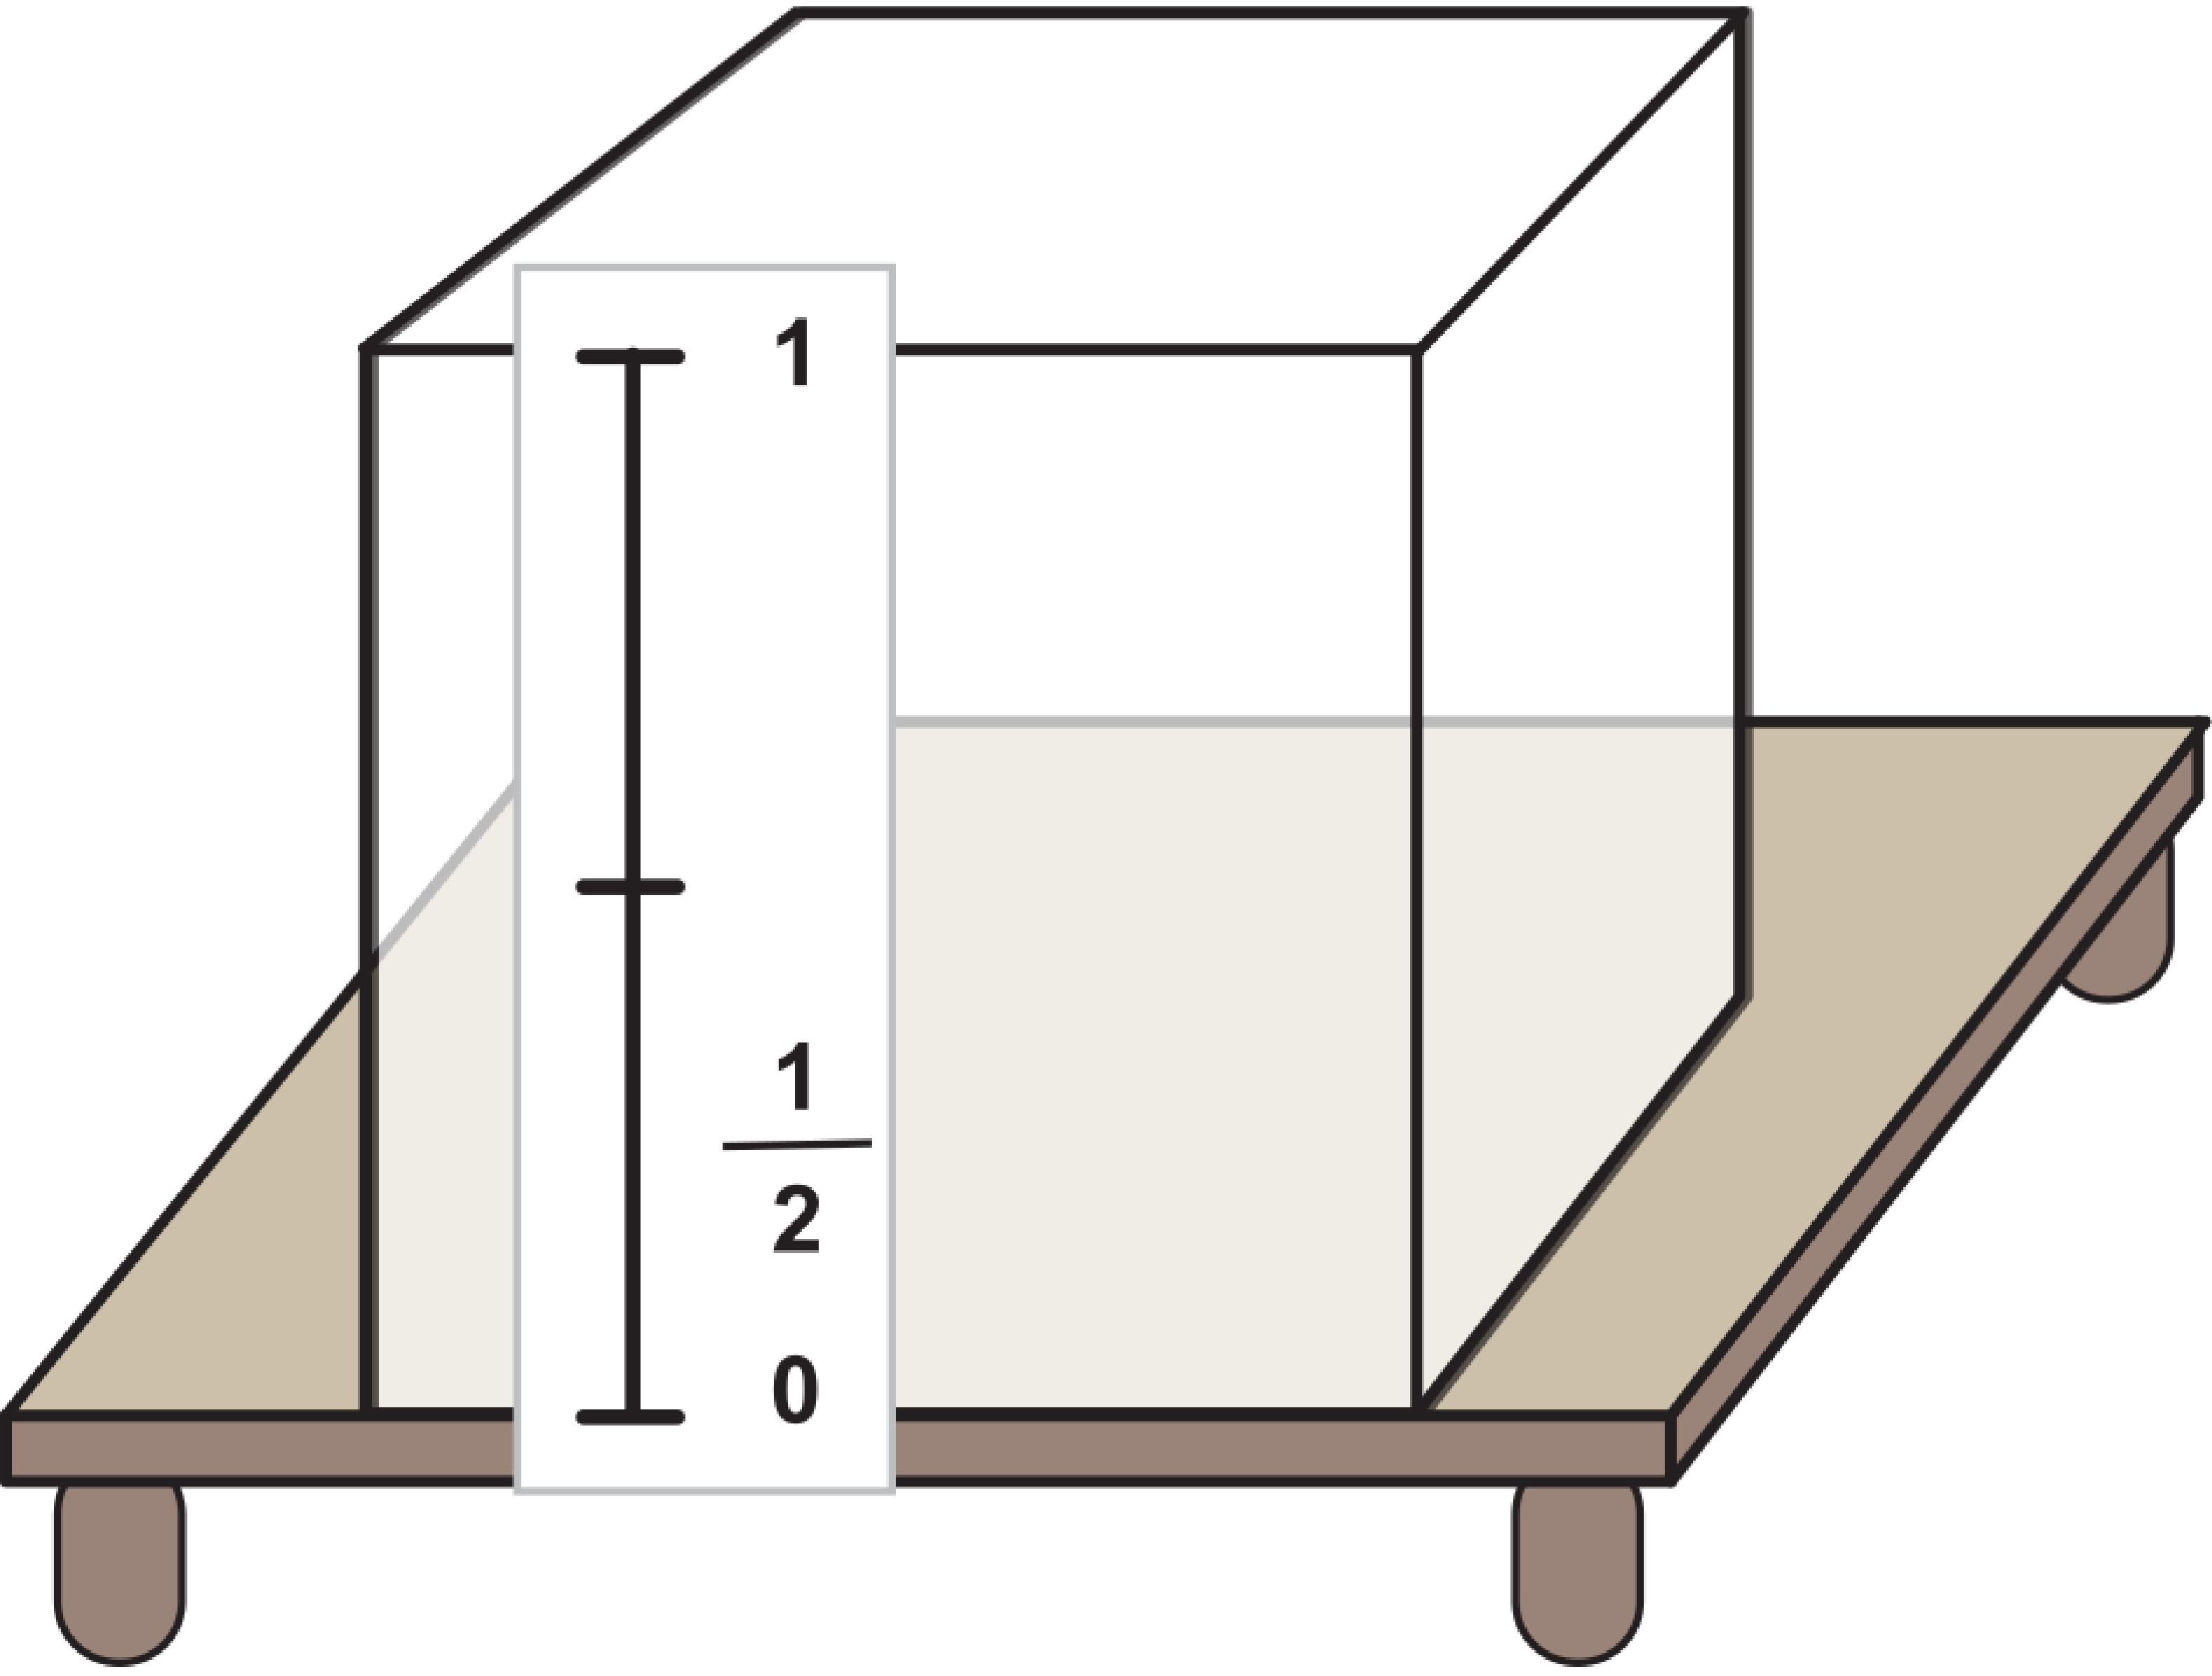
\includegraphics[width=145pt, keepaspectratio]{..//media/cap3/secoes/png/ativ1_fig05.png} &  
 \parbox[b][.3cm][t]{.3cm}{b)}  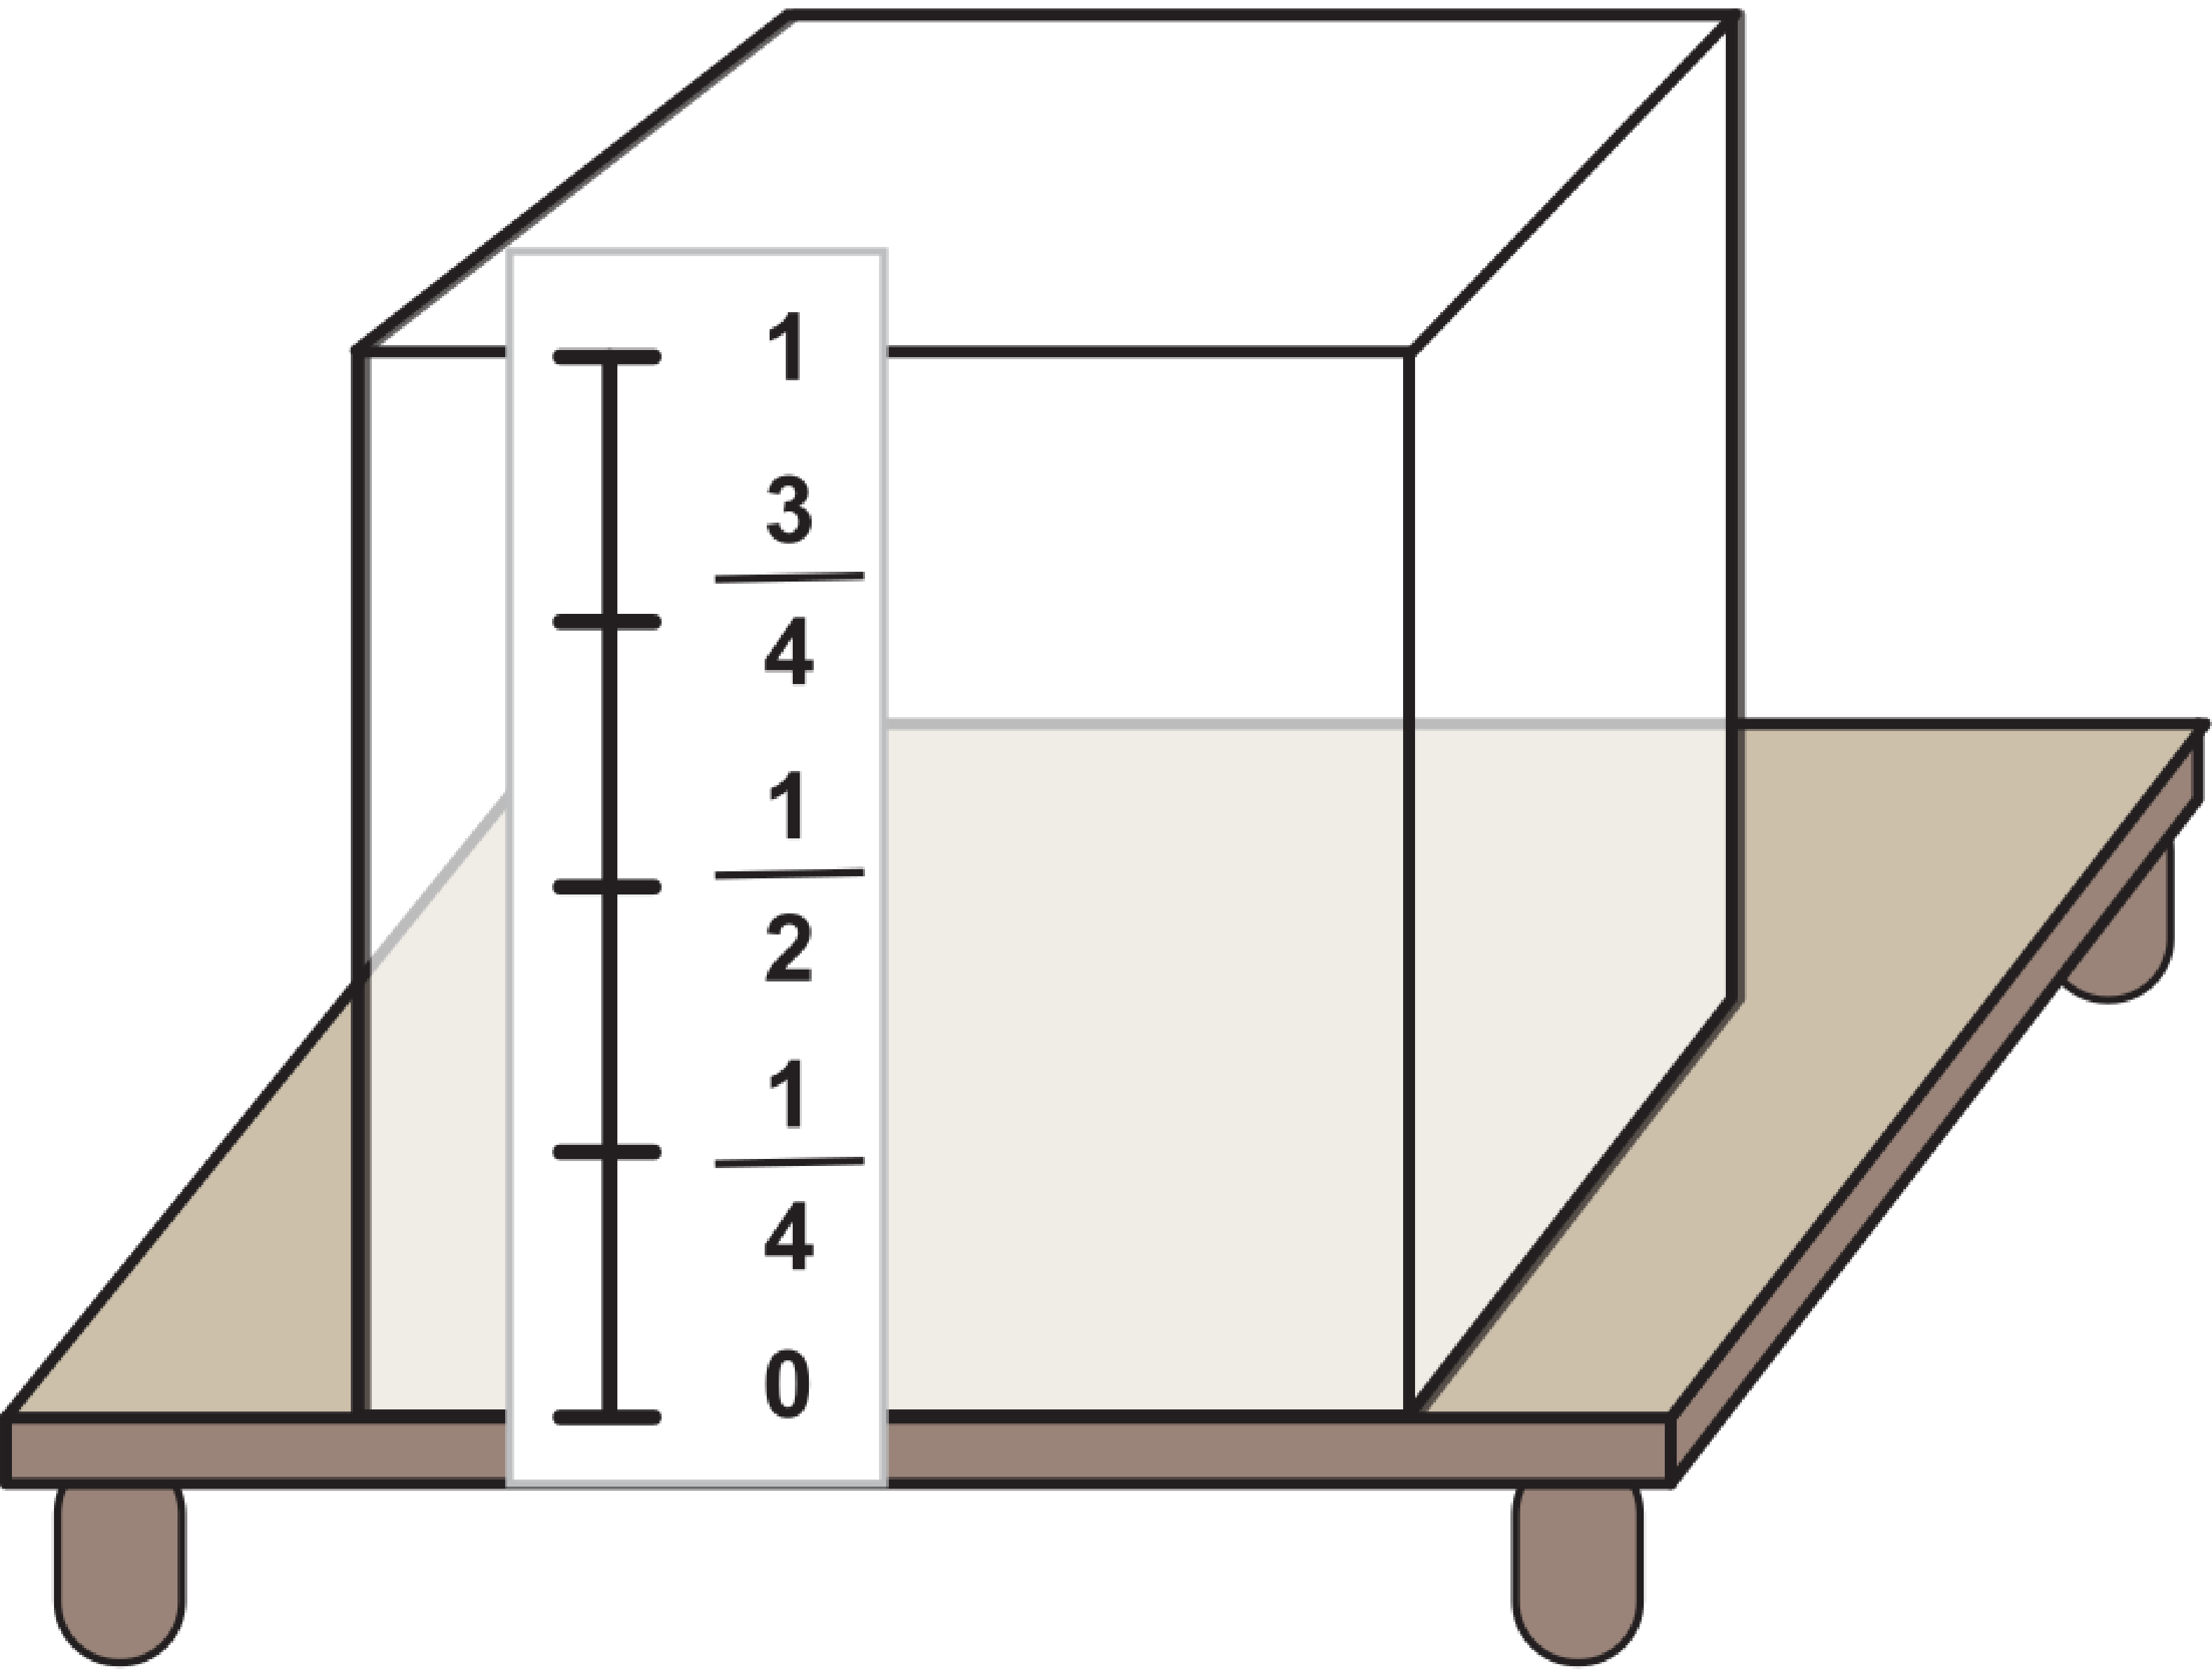
\includegraphics[width=145pt, keepaspectratio]{..//media/cap3/secoes/png/ativ1_fig06.png} &
  \parbox[b][.3cm][t]{.3cm}{c)}  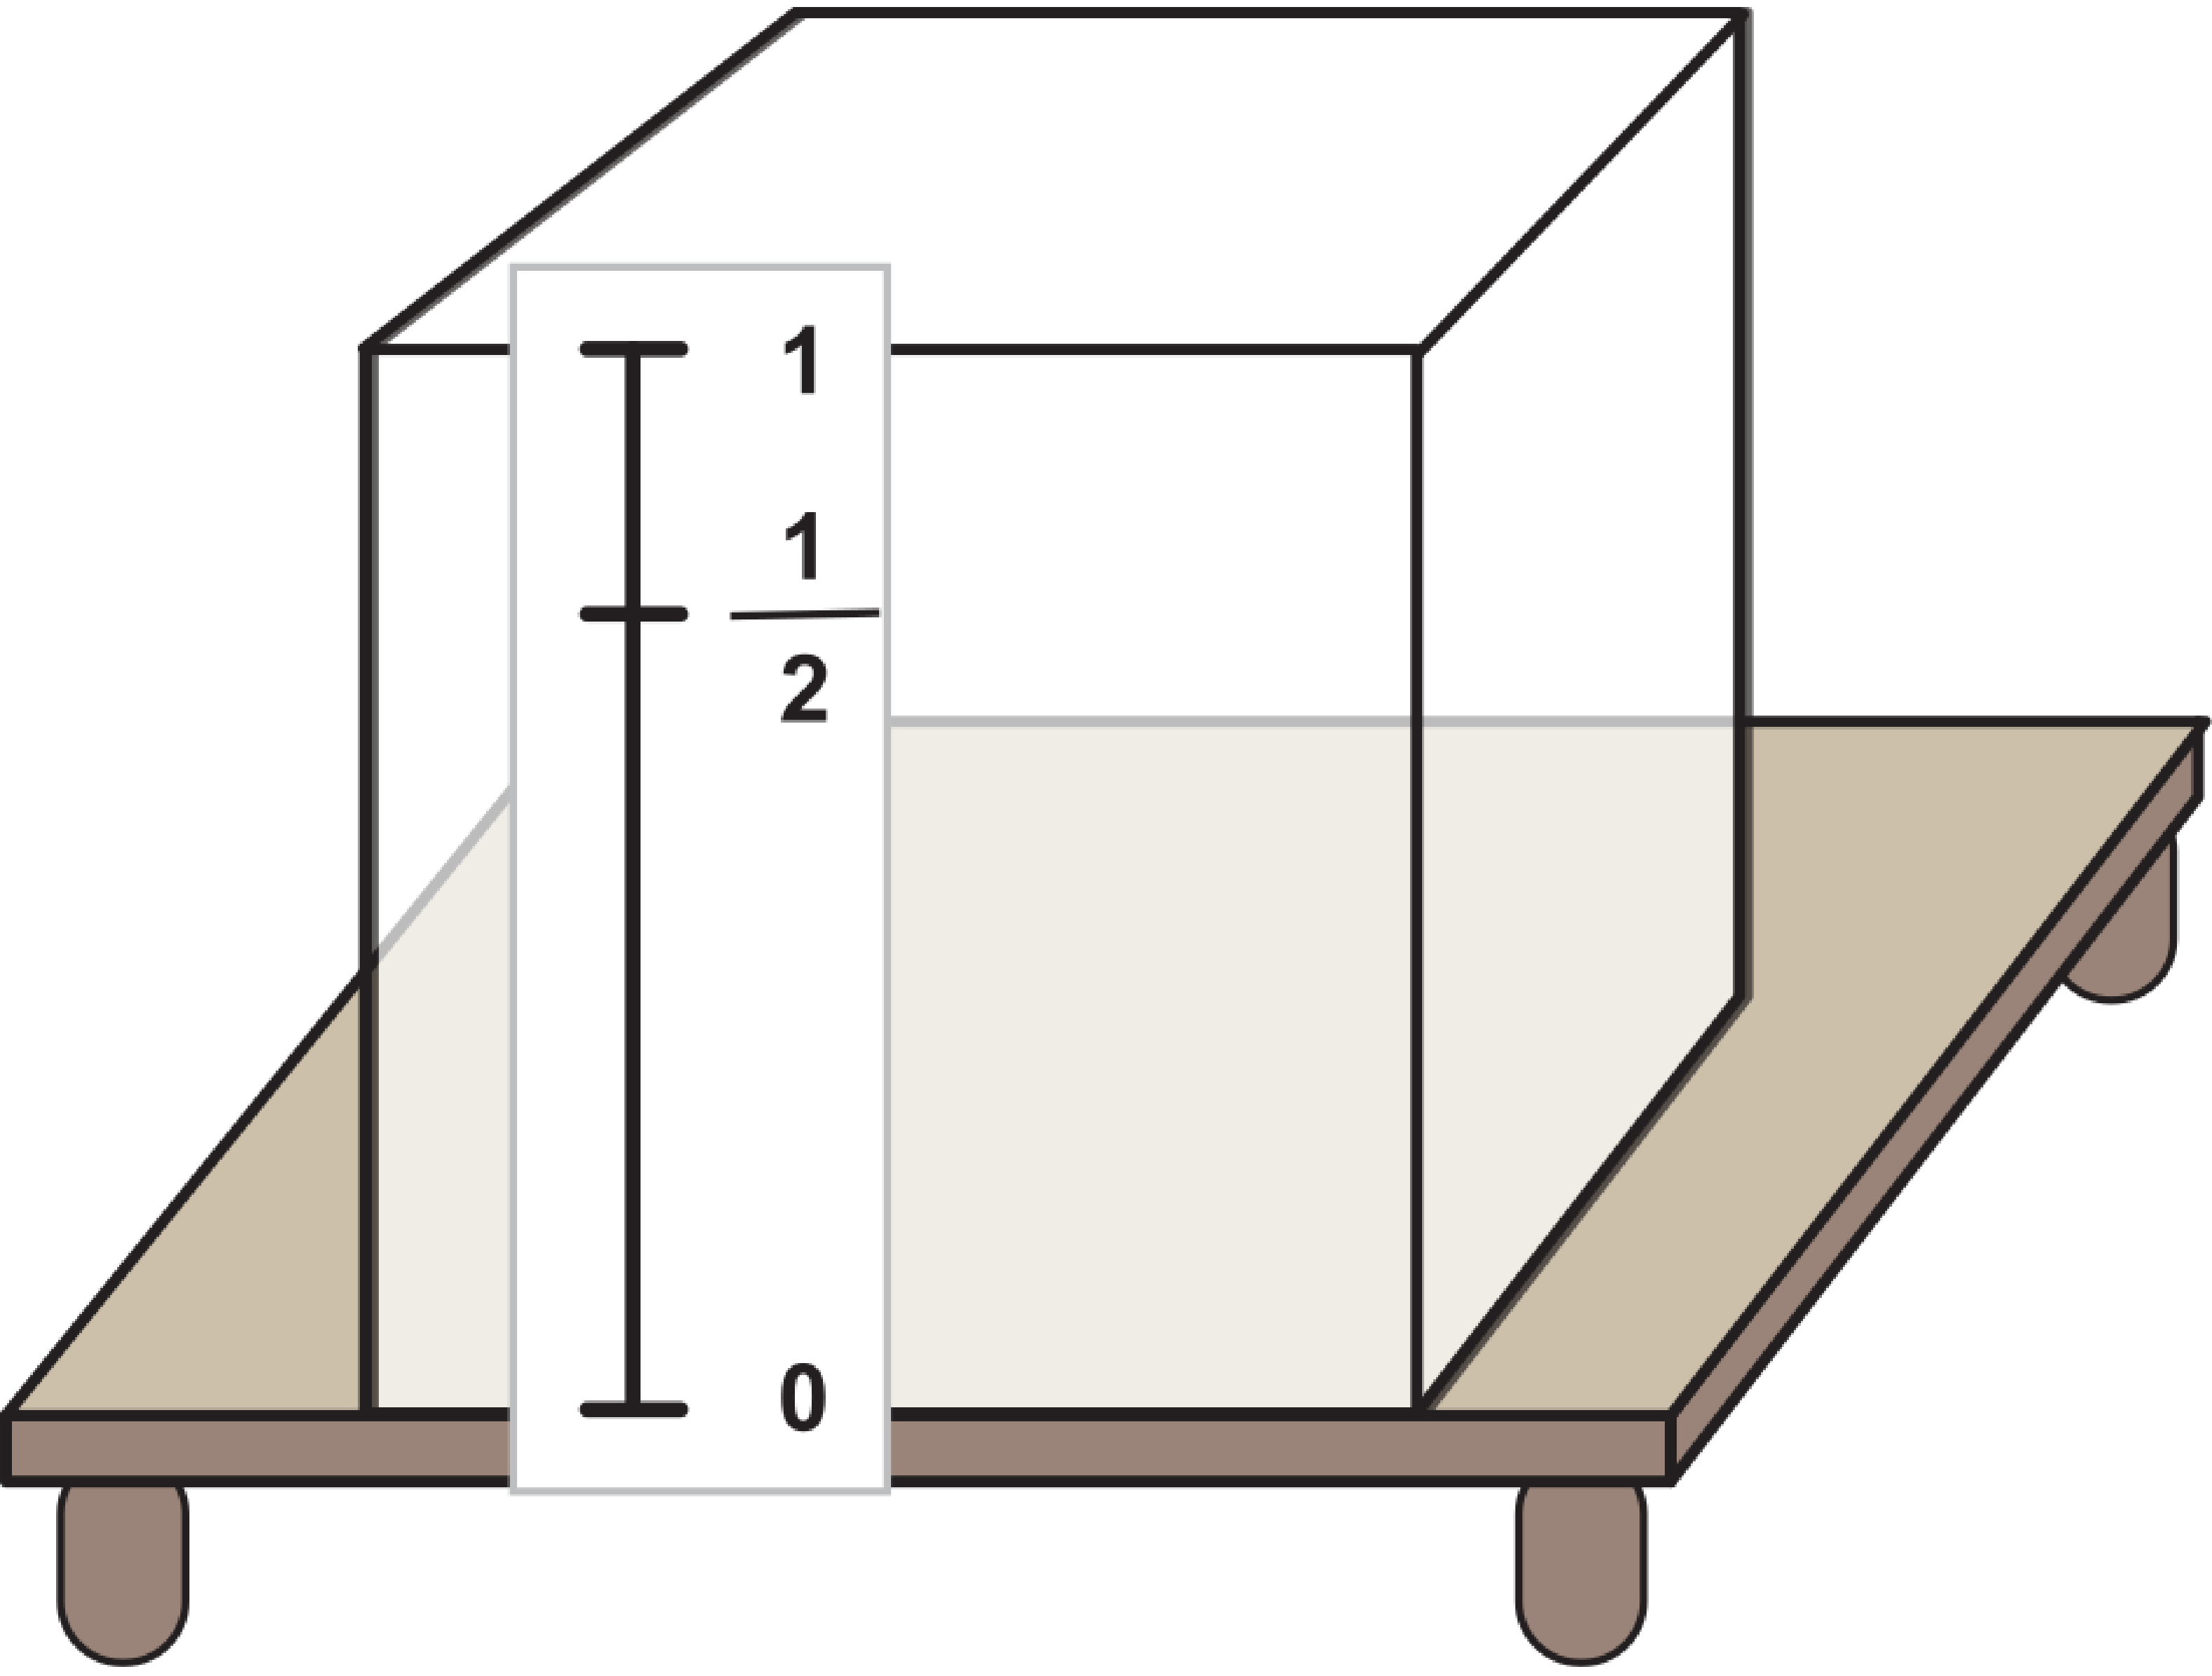
\includegraphics[width=145pt, keepaspectratio]{..//media/cap3/secoes/png/ativ1_fig07.png}  
   \end{tabular}
   
  \begin{tabular}{m{.3\textwidth}m{.3\textwidth}}
  \parbox[b][0.3cm][t]{.3cm}{d)}  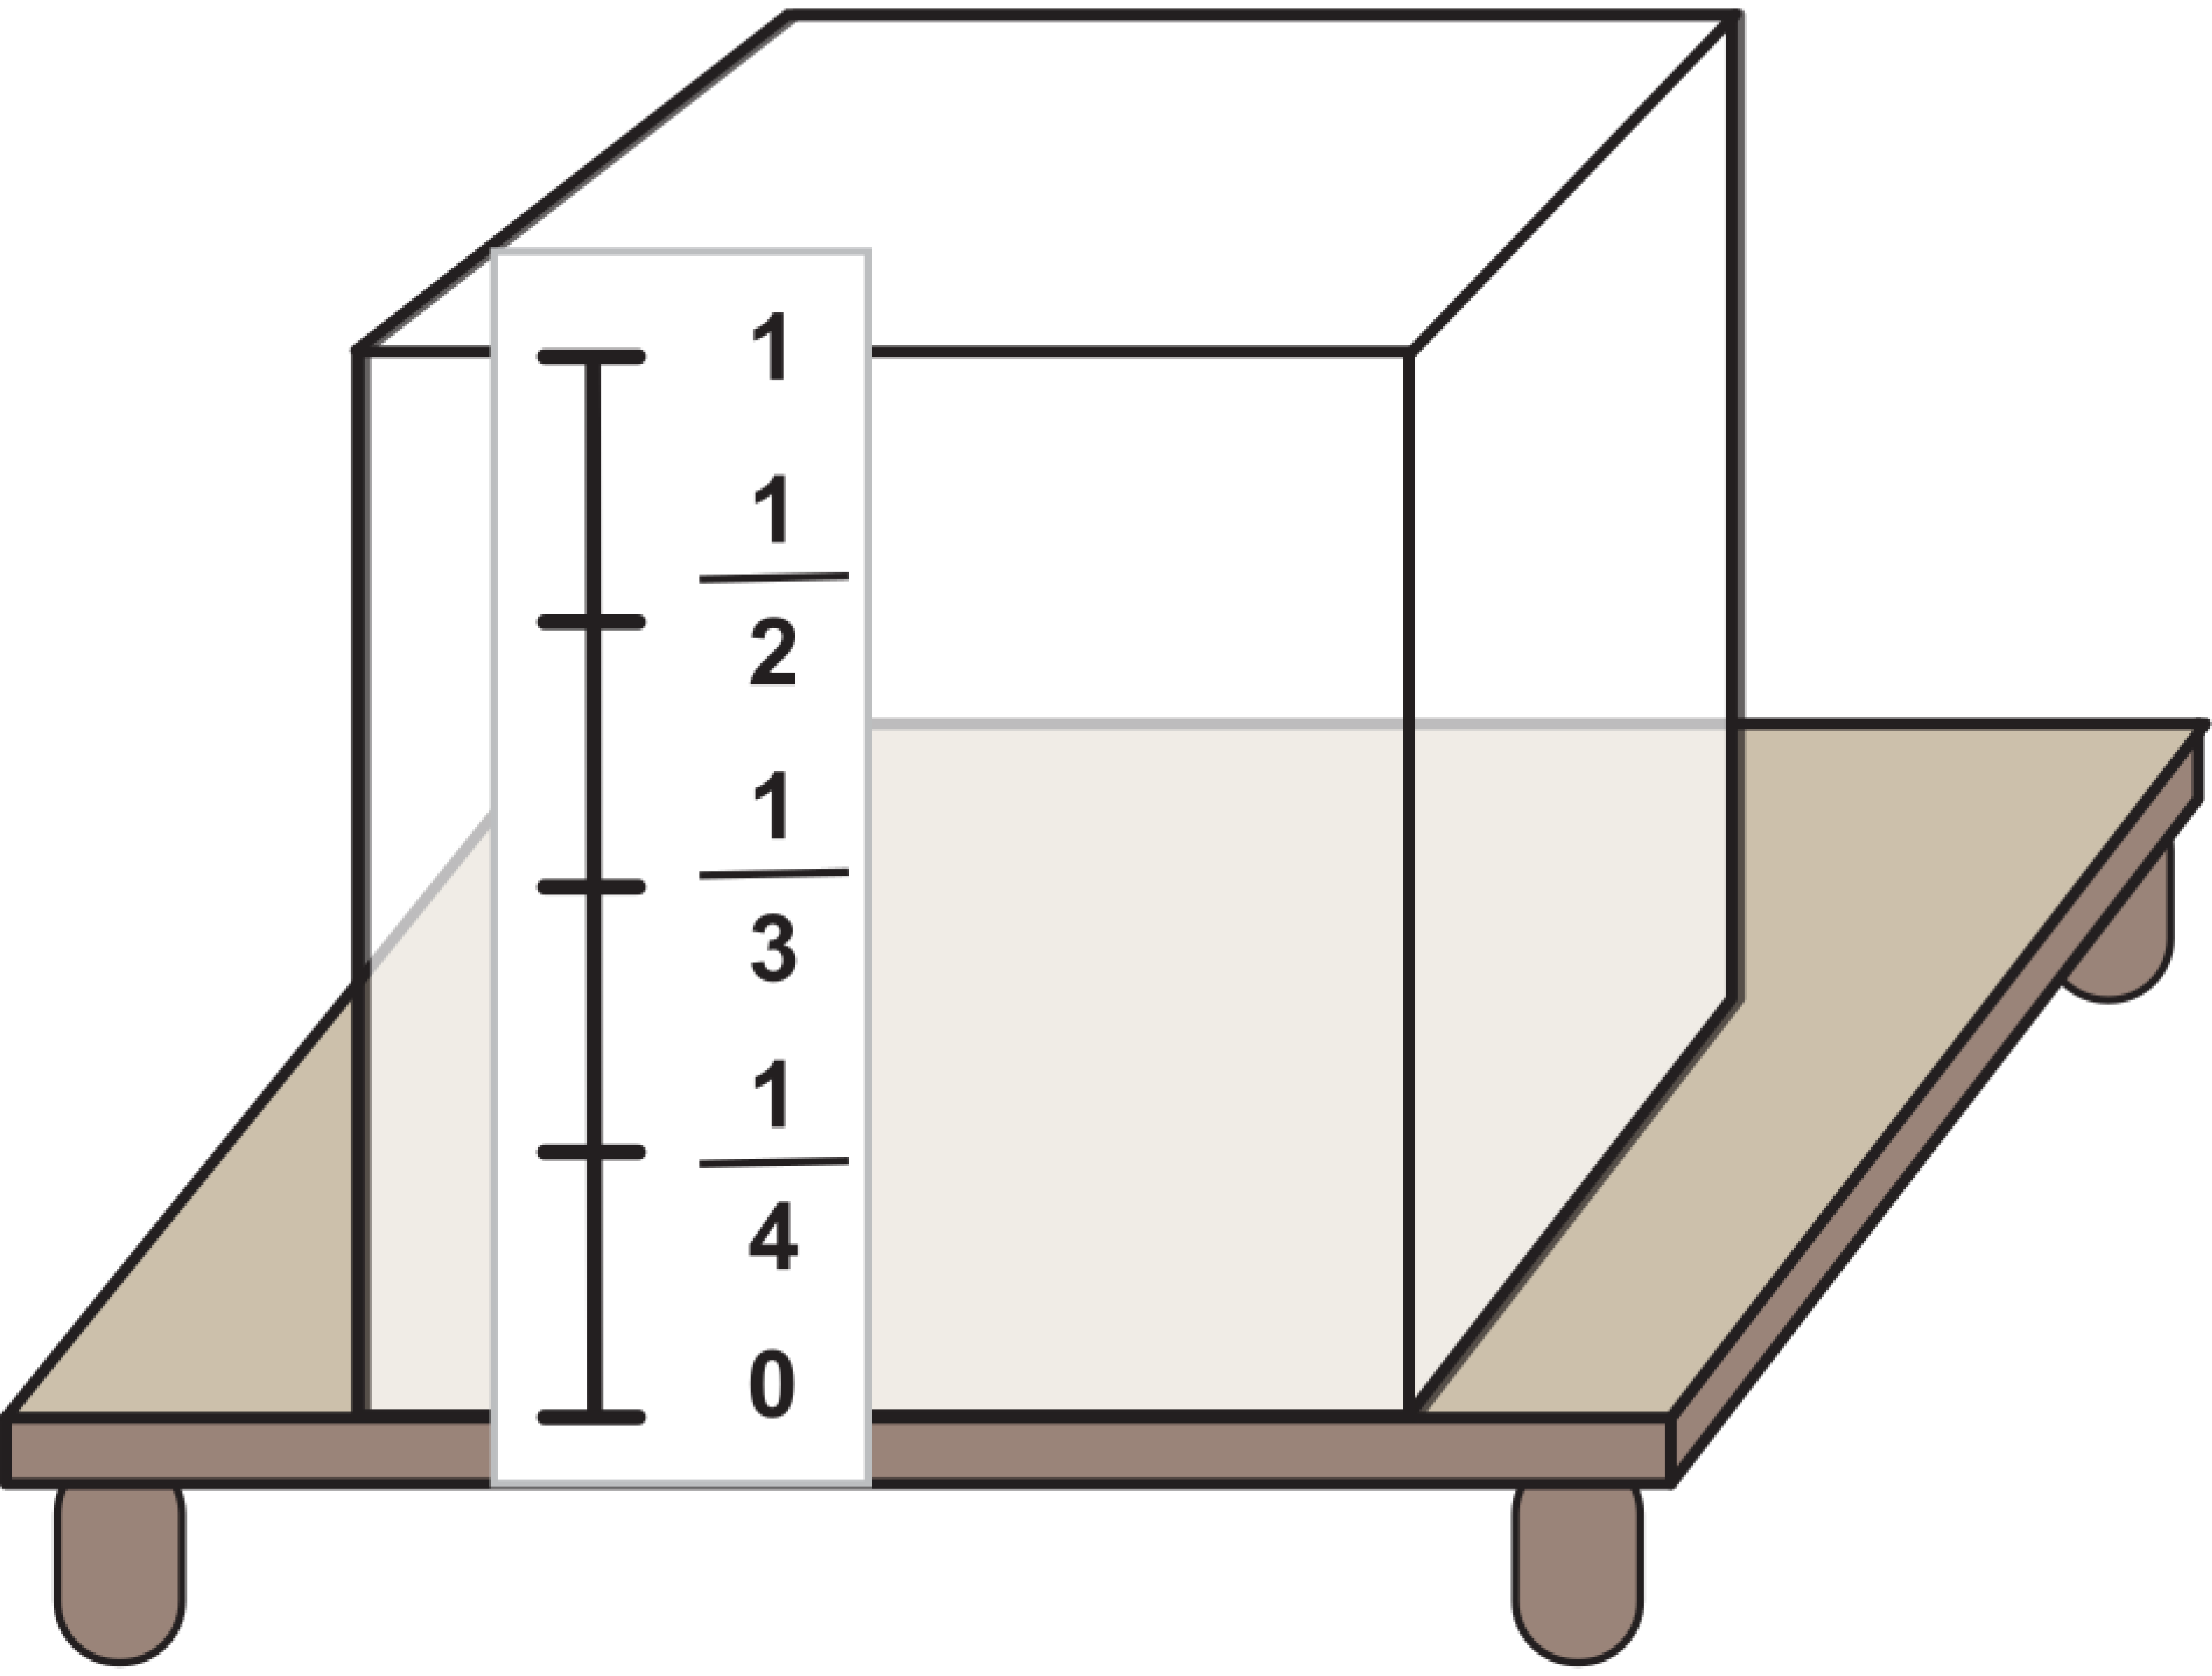
\includegraphics[width=145pt, keepaspectratio]{..//media/cap3/secoes/png/ativ1_fig08.png}&
  \parbox[b][0.3cm][t]{.3cm}{e)}  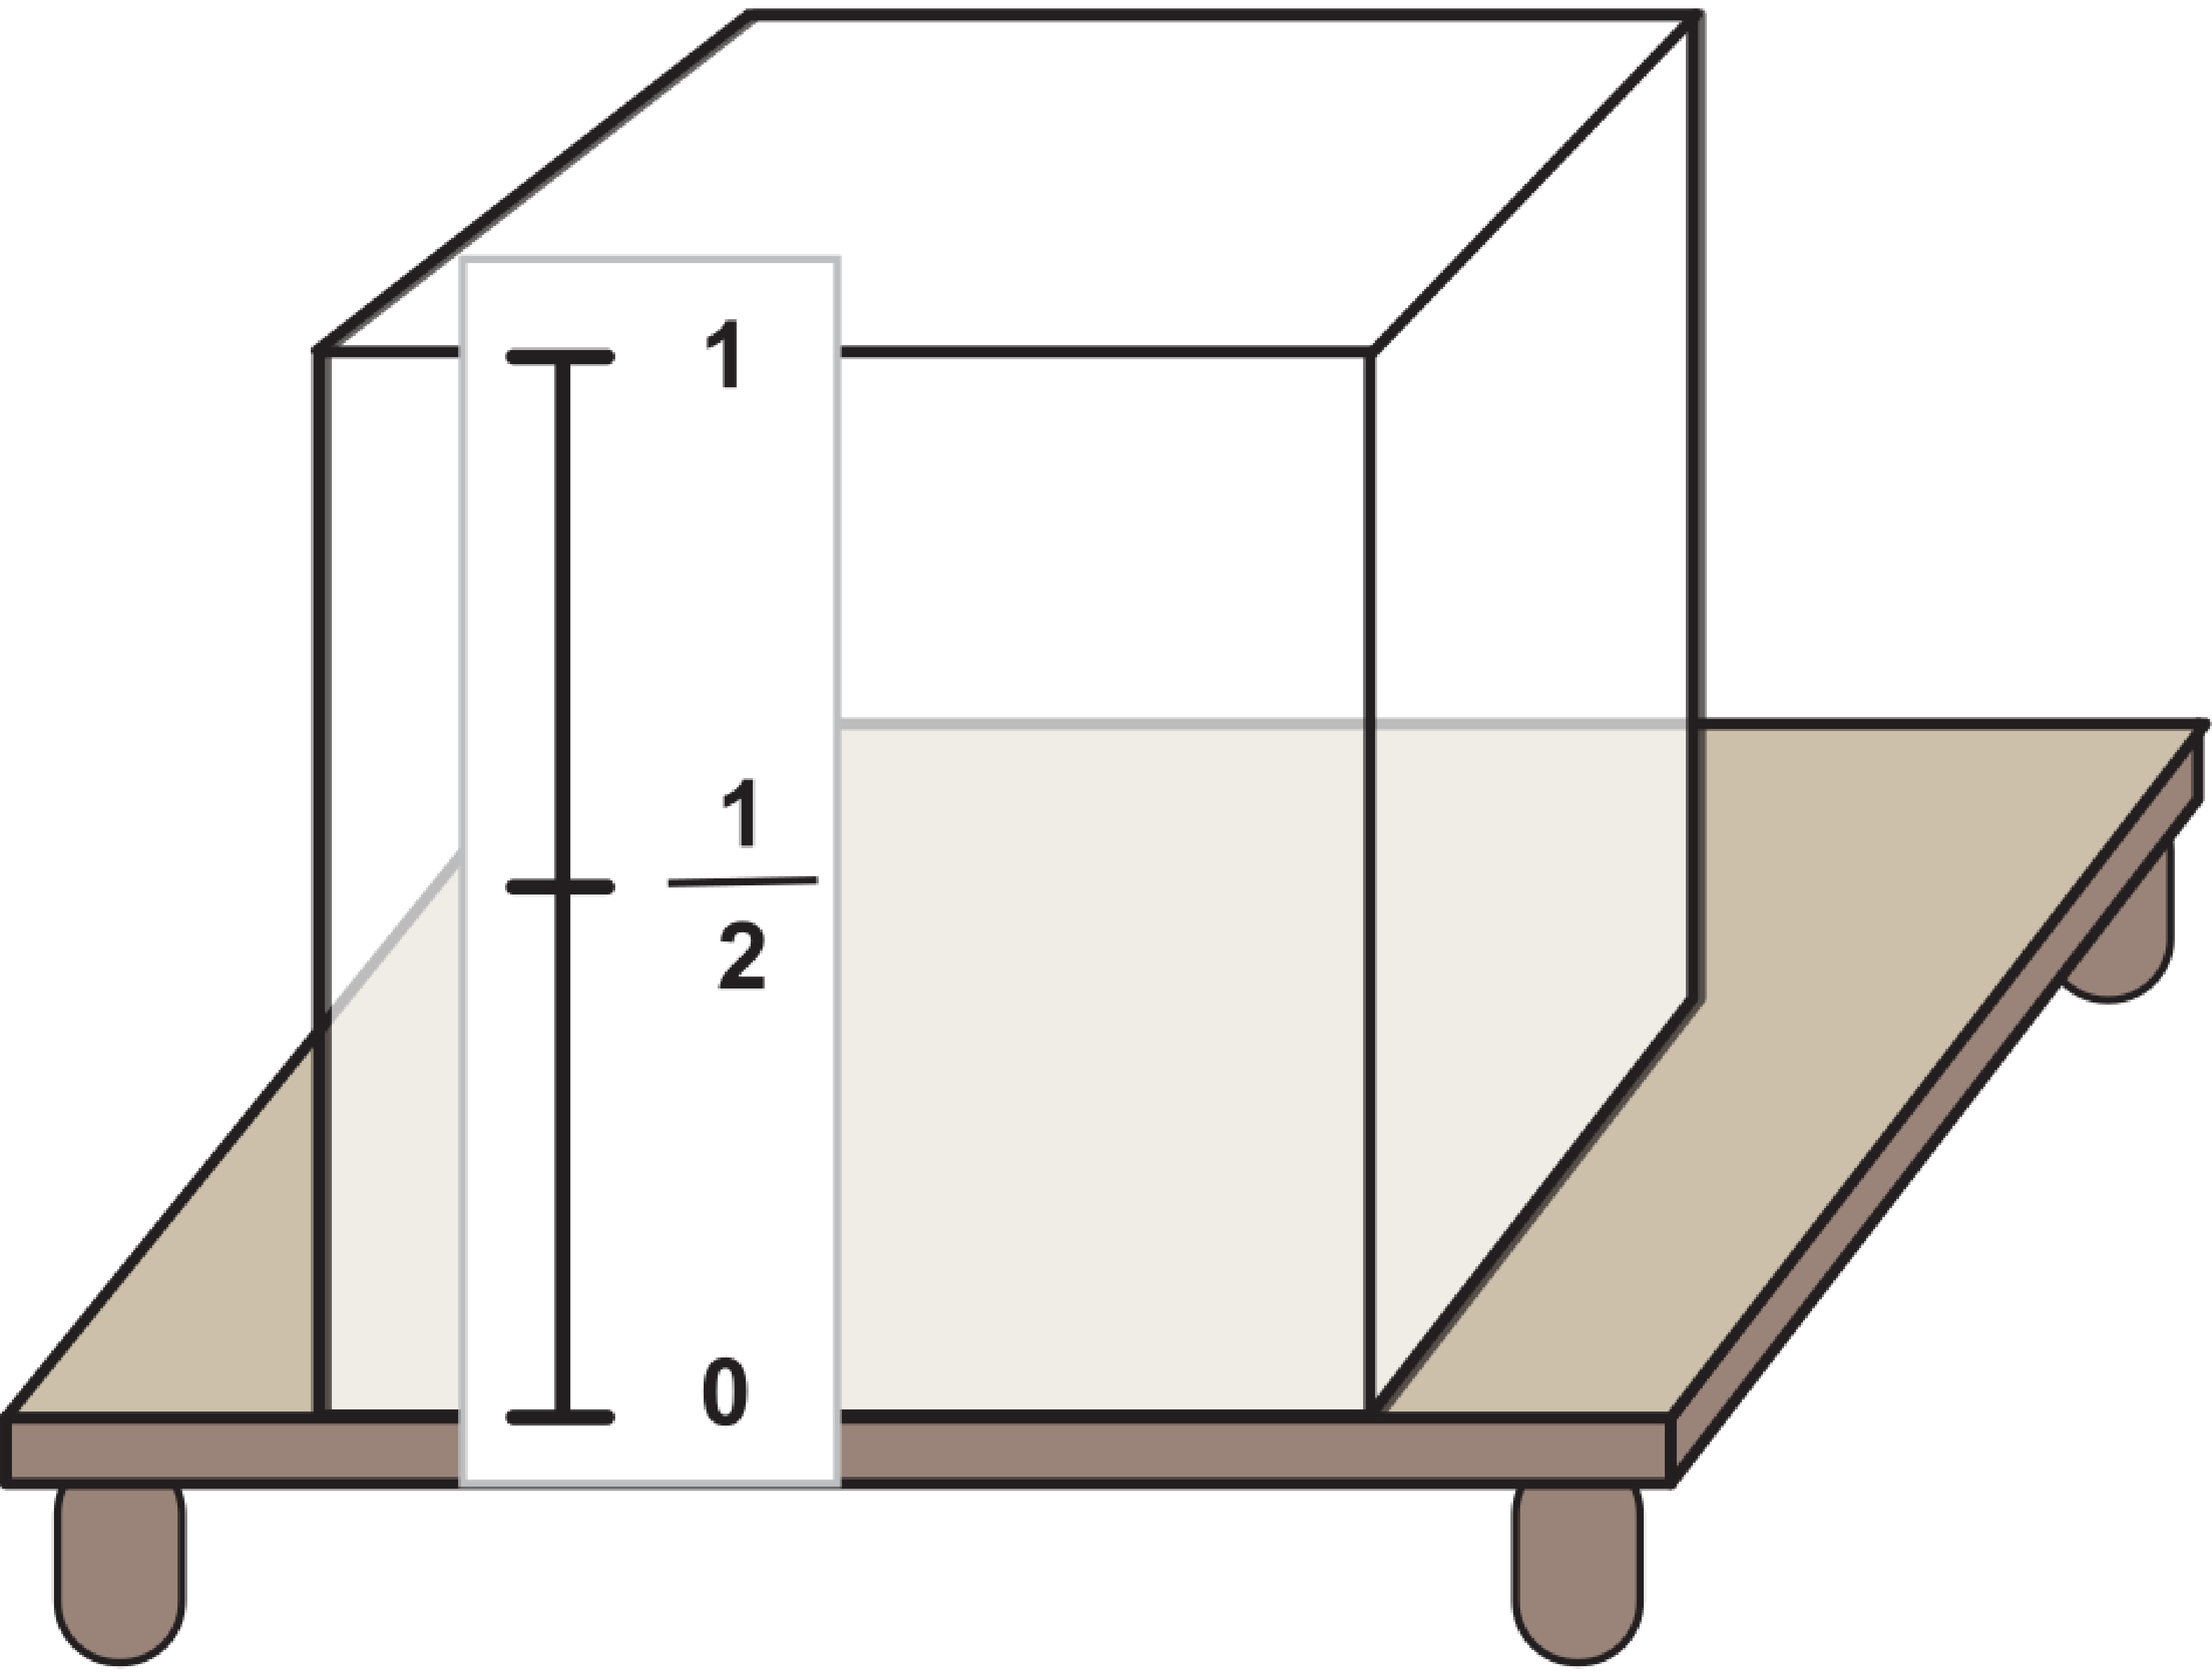
\includegraphics[width=145pt, keepaspectratio]{..//media/cap3/secoes/png/ativ1_fig09.png}
  \end{tabular}
  \end{center}

  
\subsection{Atividade}

Relembrando a representação na reta numérica: você já conhece a reta numérica com os números naturais destacados.


\begin{enumerate} [\quad a)] %s
  \item     Marque na reta numérica pontos que representem as 3 quantidades de pizza nas imagens a seguir. 

\begin{center}
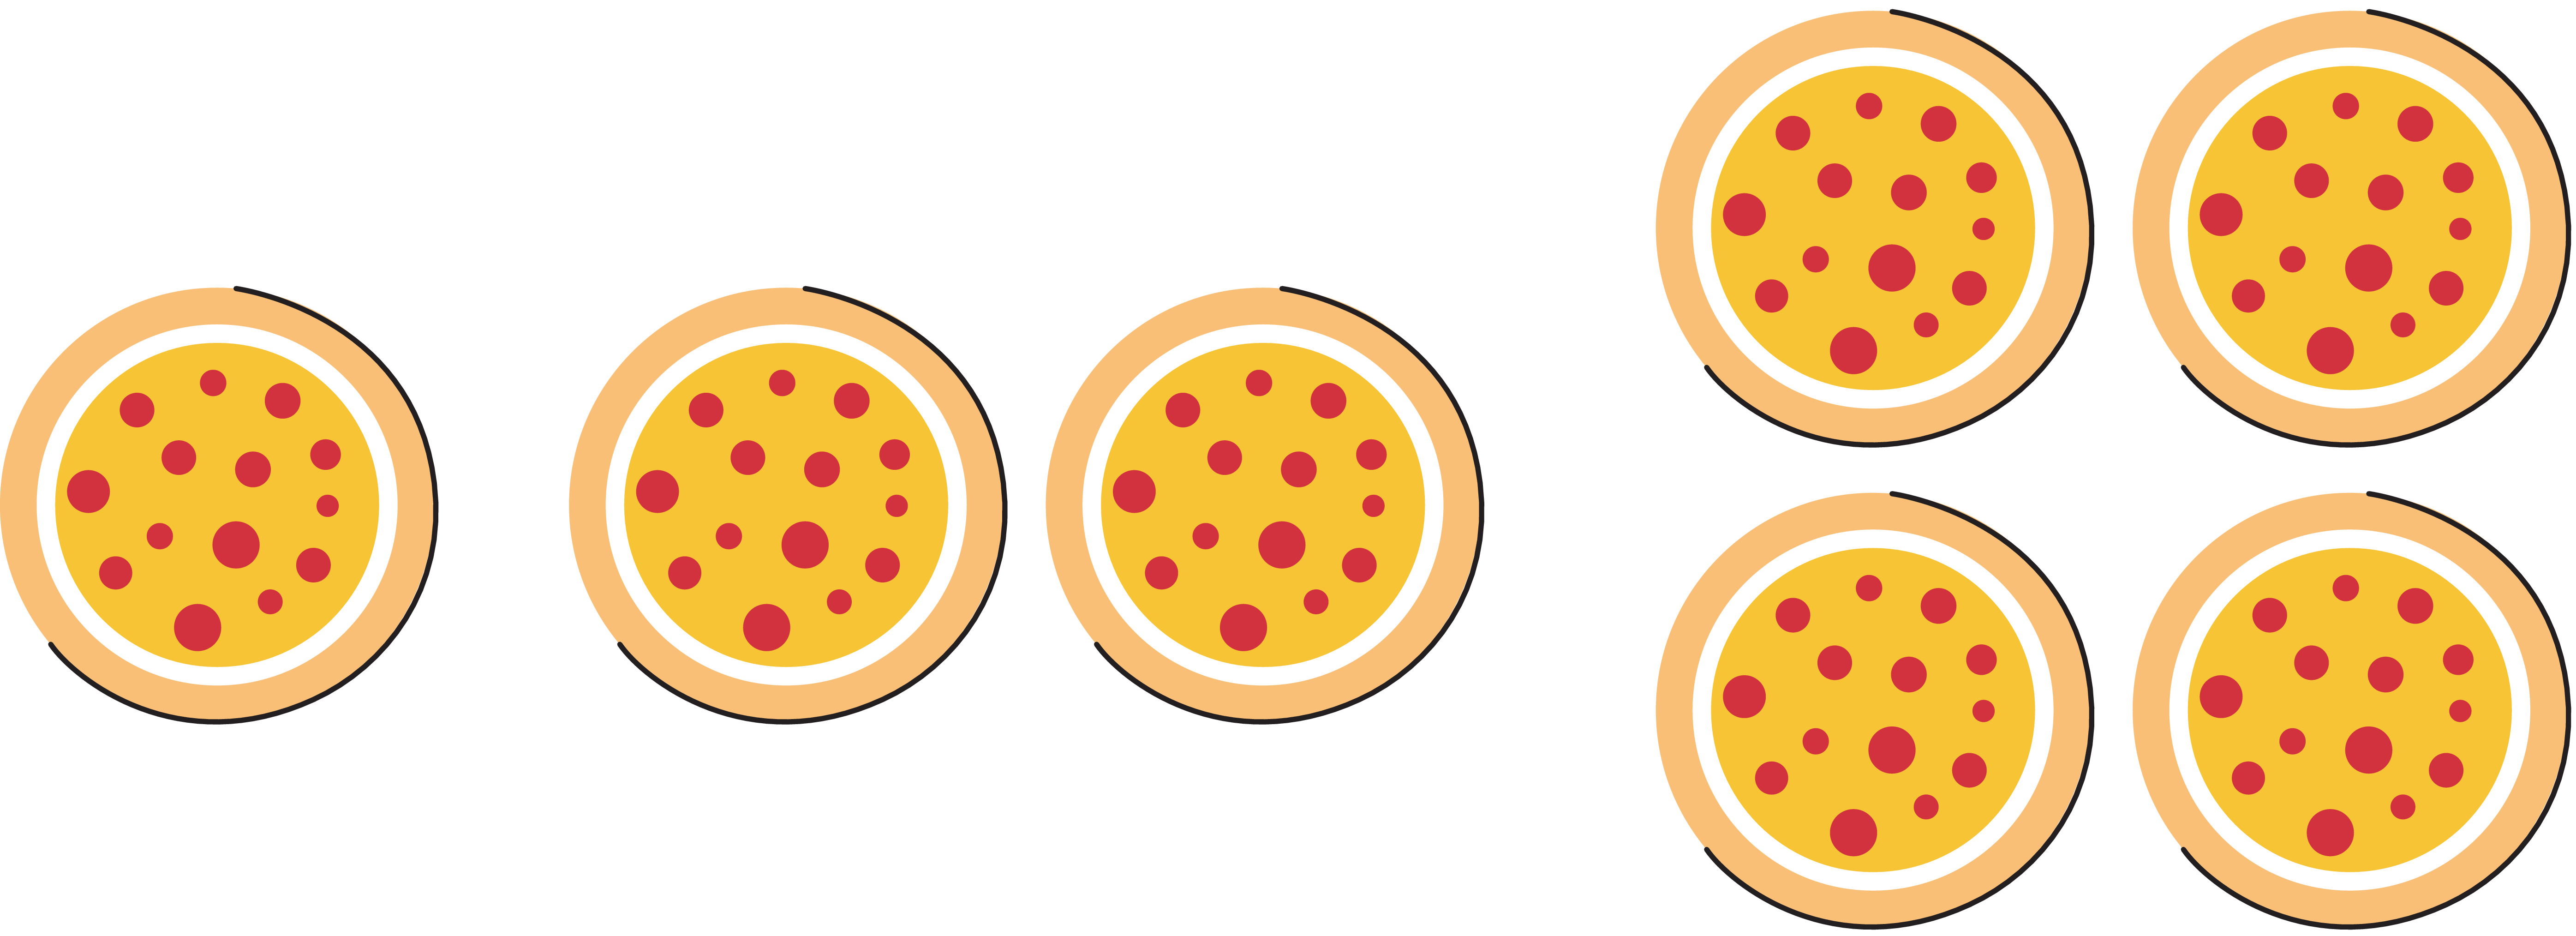
\includegraphics[width=400pt, keepaspectratio]{..//media/cap3/secoes/png/ativ2_fig_a.png} 
\end{center}

\begin{center}
\begin{tikzpicture}[x=10mm,y=10mm]
\draw[->] (-1,0) -- (6,0) ; %edit here for the axis
\foreach \x in  {0,1,...,5} % edit here for the vertical lines
\draw[shift={(\x,0)},color=black] (0,3pt) -- (0pt,-3pt) 
node[below] {$\x$};

\foreach \x in  {0.5,1.5,...,4.5} % edit here for the vertical lines
\draw[shift={(\x,0)},color=black] (0,2pt) -- (0pt,-2pt); 

\end{tikzpicture}
\end{center}

\item     E no caso destas imagens, que pontos na reta numérica representam as 4 quantidades de pizza ilustradas?
\end{enumerate} %s

\begin{center}

\includegraphics[width=400pt, keepaspectratio]{..//media/cap3/secoes/png/ativ2_fig_b2.png} 
\end{center}


  \begin{center}
  \begin{tikzpicture}[x=30mm,y=30mm]
\draw[->] (-1/4,0) -- (2.5,0) ; %edit here for the axis
\foreach \x in  {0,0.25,...,2} % edit here for the vertical lines
\draw[shift={(\x,0)},color=black] (0,3pt) -- (0pt,-3pt); 
\foreach \x in  {0,1,2}
\draw[shift={(\x,0)},color=black] (0,3pt) -- (0pt,-3pt) node[below] {$\x$};
\end{tikzpicture}
\end{center}
  
\subsection{Atividade}

Para cada par ou trio de figuras a seguir, há uma reta numérica. Considerando a região colorida de vermelho como uma fração da figura, ligue cada uma das figuras ao número, sobre a reta numérica, correspondente à região colorida da mesma.

\begin{longtable}{lccc}
 
%retangulos 
\parbox[b][2.6cm][t]{.3cm}{a)}&
 
\begin{tikzpicture}[x=30mm,y=30mm,scale=.6]
\draw[ fill=attention] (-1.8,0) rectangle (0,1.2) node[above, shift={(-.7,0)}] {Figura 1};
\end{tikzpicture}
&&
 
\begin{tikzpicture}[x=30mm,y=30mm,scale=.6]
\draw[fill=common, fill opacity=.3] (0,0) rectangle (1.8,1.2);
\node[above, black] at (.9,1.2) {Figura 2};
\draw[fill=attention] (0,0) -- (0,1.2) --(1.8,0)--cycle;
\end{tikzpicture}
 
\\
 
\multicolumn{4}{c}{
\parbox[c][.7cm][t]{8cm}{ } }
 
\\
 
&\multicolumn{3}{c}{
\begin{tikzpicture}[x=45mm,y=45mm]
\draw[->] (-0.5,0) -- (1.5,0) ; %edit here for the axis
\foreach \x in  {0,1} % edit here for the vertical lines
\draw[shift={(\x,0)},color=black] (0,3pt) -- (0pt,-3pt) 
node[below] {$\x$};
\draw[shift={(0.5,0)},color=black] (0,3pt) -- (0pt,-3pt) 
node[below] {$\frac{1}{2}$};
\end{tikzpicture}   
}
 
\\ 
\parbox[b][2.6cm][t]{.3cm}{b)}&
 
%quadrados
 
 
 \begin{tikzpicture}[x=30mm,y=30mm]
\def\scale{.6}
%
\draw[fill=common, fill opacity=.3, scale=\scale] (-1.2,0) rectangle (0,1.2);
\draw[fill=attention, scale=\scale] (-1.2,0) rectangle (-0.8,.4);
\draw[fill=attention, scale=\scale] (-.4,0) rectangle (0,.4);
\draw[fill=attention, scale=\scale] (-1.2,0.8) rectangle (-0.8,1.2);
\draw[fill=attention, scale=\scale] (-.4,0.8) rectangle (0,1.2);
\draw[fill=attention, scale=\scale] (-.8,0.4) rectangle (-0.4,.8);

% \draw[ fill=attention, scale=\scale] (-1.2,.8) rectangle (0,1.2);
 
% \draw[fill=common, fill opacity=.3, scale=\scale] (-0.8,0) rectangle (-.4,.4);
% \draw[ fill=attention, scale=\scale] (-0.8,.4) rectangle (-0.4,.8);
% \draw[fill=common, fill opacity=.3, scale=\scale] (-0.8,.8) rectangle (-.4,1.2);
\end{tikzpicture}
&&
 \begin{tikzpicture}[x=30mm,y=30mm]
\def\scale{.6}
\draw[fill=attention, scale=\scale] (0,0) rectangle (1.2,1.2);
\end{tikzpicture}
 
\\
 
\multicolumn{4}{c}{
\parbox[c][.7cm][t]{8cm}{ } }
 
\\
 
&\multicolumn{3}{c}{
\begin{tikzpicture}[x=45mm,y=45mm]
\draw[->] (-0.5,0) -- (1.5,0) ; %edit here for the axis
\foreach \x in  {0,0.1111,...,1}{ % edit here for the vertical lines
\draw[shift={(\x,0)},color=black] (0,3pt) -- (0pt,-3pt);} 
\foreach \x in  {0,1}
\draw[shift={(\x,0)},color=black] (0,3pt) -- (0pt,-3pt) node[below] {$\x$};
\foreach \x in  {3,5}
\draw[shift={(\x/9,0)},color=black] (0,3pt) -- (0pt,-3pt) node[below] {$\frac{\x}{9}$};
\end{tikzpicture}}
\\ 
 
%hexagonos
\parbox[b][2.6cm][t]{.3cm}{c)}&
 
\begin{tikzpicture}[x=30mm,y=30mm]
\def\scale{.6}% to rescale the polygons only.
 
%hexagon on the left
\fill[shift={(0,0.6)}, fill=attention, scale=\scale] (0,0) -- (90:0.7) -- (150:0.7)-- (210:.7);
\fill[shift={(0,0.6)}, fill=common, fill opacity=.3, scale=\scale] (0,0) -- (90:0.7) -- (30:0.7)-- (-30:.7) -- (-90:.7) -- (-150:.7)--cycle;
\foreach \x in {30,90,...,330}{
\draw[shift={(0,0.6)}, scale=\scale] (\x:0.7) -- (\x + 60: 0.7);
\draw[shift={(0,0.6)}, scale=\scale] (0,0) -- (\x:0.7);}
\end{tikzpicture}
&&
\begin{tikzpicture}[x=30mm,y=30mm] 
\def\scale{.6}% to rescale the polygons only.
 
%hexagon on the right
\foreach \x in {30,90,...,330}{
\draw[shift={(1,0.6)}, fill=attention,attention, scale=\scale] (\x:0.7) -- (\x + 60: 0.7) --(0,0) --cycle;
\draw[shift={(1,0.6)}, fill=attention, scale=\scale] (\x:0.7) -- (\x + 60: 0.7);}
\end{tikzpicture}
 
\\
 
\multicolumn{4}{c}{
\parbox[c][.7cm][t]{8cm}{ } }
 
\\
&\multicolumn{3}{c}{
\begin{tikzpicture}[x=68mm,y=68mm]
\draw[->] (-1/6,0) -- (1+1/6,0) ; %edit here for the axis
\foreach \x in  {0,0.1667,...,1}{ % edit here for the vertical lines
\draw[shift={(\x,0)},color=black] (0,3pt) -- (0pt,-3pt);} 
\foreach \x in  {0,1}
\draw[shift={(\x,0)},color=black] (0,3pt) -- (0pt,-3pt) node[below] {$\x$};
\foreach \x in  {1,2}
\draw[shift={(\x/3,0)},color=black] (0,3pt) -- (0pt,-3pt) node[below] {$\frac{\x}{3}$};
\end{tikzpicture} }
\\ 
 
\parbox[b][2.6cm][t]{.3cm}{d)}&
 
 %triangulos
\begin{tikzpicture}[x=30mm,y=30mm]
\def\scale{.6}% to rescale the polygons only.
 
\foreach \x in {90,210,330}{
\draw[attention,fill=attention, shift={(0,0.6)}, scale=\scale] (\x:0.7) -- (\x + 120: 0.7) -- (0,0)--cycle;
\draw[shift={(0,0.6)}, scale=\scale] (\x:0.7) -- (\x + 120: 0.7);}
\draw[shift={(0,0.6)}, scale=\scale] (-90:0.35) -- (30: 0.35) -- (150: 0.35) -- cycle;
\end{tikzpicture}
&&
\begin{tikzpicture}[x=30mm,y=30mm]
\def\scale{.6}% to rescale the polygons only.
\fill[shift={(1,0.6)}, scale=\scale, common, fill opacity=.3] (90:0.7) -- (210: 0.7)--(330:.7)--cycle;
\foreach \x in {90,210,330}{
\draw[shift={(1,0.6)}, scale=\scale] (\x:0.7) -- (\x + 120: 0.7);}
\draw[fill=attention, shift={(1,0.6)}, scale=\scale] (-90:0.35) -- (30: 0.35) -- (150: 0.35) -- cycle;
\end{tikzpicture}
 
\\
 
\multicolumn{4}{c}{
\parbox[c][.7cm][t]{8cm}{ } }
 
\\
&\multicolumn{3}{c}{
\begin{tikzpicture}[x=60mm,y=60mm]
\draw[->] (-1/4,0) -- (1+1/4,0) ; %edit here for the axis
\foreach \x in  {0,0.25,...,1}{ % edit here for the vertical lines
\draw[shift={(\x,0)},color=black] (0,3pt) -- (0pt,-3pt);} 
\foreach \x in  {0,1}
\draw[shift={(\x,0)},color=black] (0,3pt) -- (0pt,-3pt) node[below] {$\x$};
\foreach \x in  {1,3}
\draw[shift={(\x/4,0)},color=black] (0,3pt) -- (0pt,-3pt) node[below] {$\frac{\x}{4}$};
\end{tikzpicture}}
\\
 
\parbox[b][2.6cm][t]{.3cm}{e)}&
 
%os baianos e os novos retangulos
\begin{tikzpicture} [x=30mm,y=30mm]
\def\scalefig {.6}
\draw[shift={(-.35*\scalefig,0.3)}, fill=attention, scale=\scalefig] (-1.5,0) rectangle (-0.5,1.2) node[above, shift={(-.25*\scalefig,0)}] {Figura 1};
\draw[shift={(-.35*\scalefig,0.3)}, scale=\scalefig, fill=common, fill opacity=.3] (-.5,0) rectangle (0,1.2);
\draw[shift={(-.35*\scalefig,0.3)}, scale=\scalefig] (-1,0) -- (-1,1.2);
\end{tikzpicture}
&
\begin{tikzpicture} [x=30mm,y=30mm] 
\def\scalefig {.6}
\draw[shift={(1.25*\scalefig,0.3)}, fill=attention, scale=\scalefig] (-1.5,0) rectangle (-1,1.2);
\draw[shift={(1.25*\scalefig,0.3)}, scale=\scalefig, fill=common, fill opacity=.3] (-1,0) rectangle (0,1.2); 
\node[shift={(1.25*\scalefig,0.3)}] at (-.48,.85) {Figura 2};
\draw[shift={(1.25*\scalefig,0.3)}, scale=\scalefig] (-.5,0) -- (-.5,1.2);
\end{tikzpicture}
&
\begin{tikzpicture} [x=30mm,y=30mm] 
\def\scalefig {.6}
\draw[shift={(1.35*\scalefig,0.3)}, fill=attention, scale=\scalefig] (0,0) rectangle (1.5,1.2) node[above, shift={(-.75*\scalefig,0)}] {Figura 3};
\draw[shift={(1.35*\scalefig,0.3)}, scale=\scalefig] (.5,0) -- (.5,1.2);
\draw[shift={(1.35*\scalefig,0.3)}, scale=\scalefig] (1,0) -- (1,1.2);
\end{tikzpicture}
 
\\
 
\multicolumn{4}{c}{
\parbox[c][.7cm][t]{8cm}{ } }
 
\\
&\multicolumn{3}{c}{
\begin{tikzpicture}[x=55mm,y=55mm]
 \begin{scope}[shift={(-.3,0)}]
\draw[->] (-1/3,0) -- (1.33,0) ; %edit here for the axis
\foreach \x in  {0,1} % edit here for the vertical lines
\draw[shift={(\x,0)},color=black] (0,3pt) -- (0pt,-3pt) 
node[below] {$\x$};
\foreach \x in {1,2}
\draw[shift={(\x/3,0)},color=black] (0,3pt) -- (0pt,-3pt) 
node[below] {$\frac{\x}{3}$};
\end{scope}
\end{tikzpicture}}
\\
\parbox[b][2.6cm][t]{.3cm}{f)}&
 
\begin{tikzpicture}[scale=.48]
\fill[common, fill opacity=.3] (0,0) rectangle (45,45); 
 \fill[attention] (0,33.75) rectangle (33.75,45);
 \draw[step=11.25, fill=attention] (0,0) grid (45,45); 
\end{tikzpicture}
&
\begin{tikzpicture}[scale=.48]
\draw[fill=attention] (0,0) rectangle (45,45);
\end{tikzpicture}
&
 
\begin{tikzpicture}[scale=.48]
  \draw[step=11.25, fill=attention] (0,0) rectangle (45,45); 
  \draw[step=11.25, fill=white] (11.25,0) rectangle (45,11.25);
  \draw[step=11.25, fill=common, fill opacity=.3] (11.25,0) rectangle (45,11.25);
  \draw[step=11.25] (0,0) grid (45,45); 
\end{tikzpicture}
\\
 
\multicolumn{4}{c}{
\parbox[c][.7cm][t]{8cm}{ } }
 
\\
&\multicolumn{3}{c}{
\begin{tikzpicture}[x=90mm,y=90mm]
 \draw[->] (-1/16,0) -- (1+1/16,0) ; %edit here for the axis
 \foreach \x in  {0,0.0625,...,1}{ % edit here for the vertical lines
 \draw[shift={(\x,0)},color=black] (0,3pt) -- (0pt,-3pt);} 
\foreach \x in  {0,1}
\draw[shift={(\x,0)},color=black] (0,3pt) -- (0pt,-3pt) node[below] {$\x$};
\foreach \x in  {3,7,10,13}
\draw[shift={(\x/16,0)},color=black] (0,3pt) -- (0pt,-3pt) node[below] {$\frac{\x}{16}$};
\end{tikzpicture}
}
\end{longtable}

\subsection{Atividade}

Para cada uma das figuras a seguir, marque na reta numérica o ponto correspondente à fração da unidade destacada na imagem:


\begin{enumerate} [\quad a)] %s
  \item     A unidade é uma pizza. 

\begin{center}
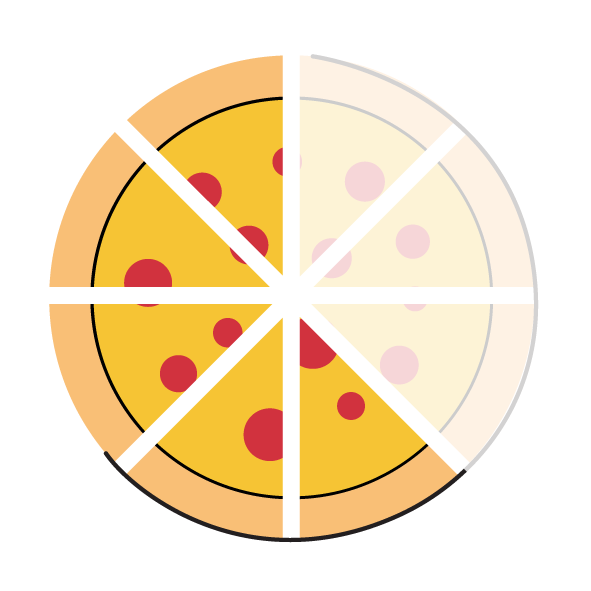
\includegraphics[width=60pt, keepaspectratio]{..//media/cap3/secoes/png/ativ4_fig_a.png} 
\quad\quad\quad \begin{tikzpicture}[x=56.25mm,y=56.25mm]
\draw[->] (-0.3,0) -- (1.3,0) ; %edit here for the axis
\foreach \x in  {0,1} % edit here for the vertical lines
\draw[shift={(\x,0)},color=black] (0,3pt) -- (0pt,-3pt) 
node[below] {$\x$};
 
\foreach \x in {3,5}
\draw[shift={(\x/8,0)},color=black] (0,3pt) -- (0pt,-3pt) 
node[below] {$\frac{\x}{8}$};
\end{tikzpicture}   
\end{center}

\item     A unidade é uma barra de chocolate. 

\begin{center}
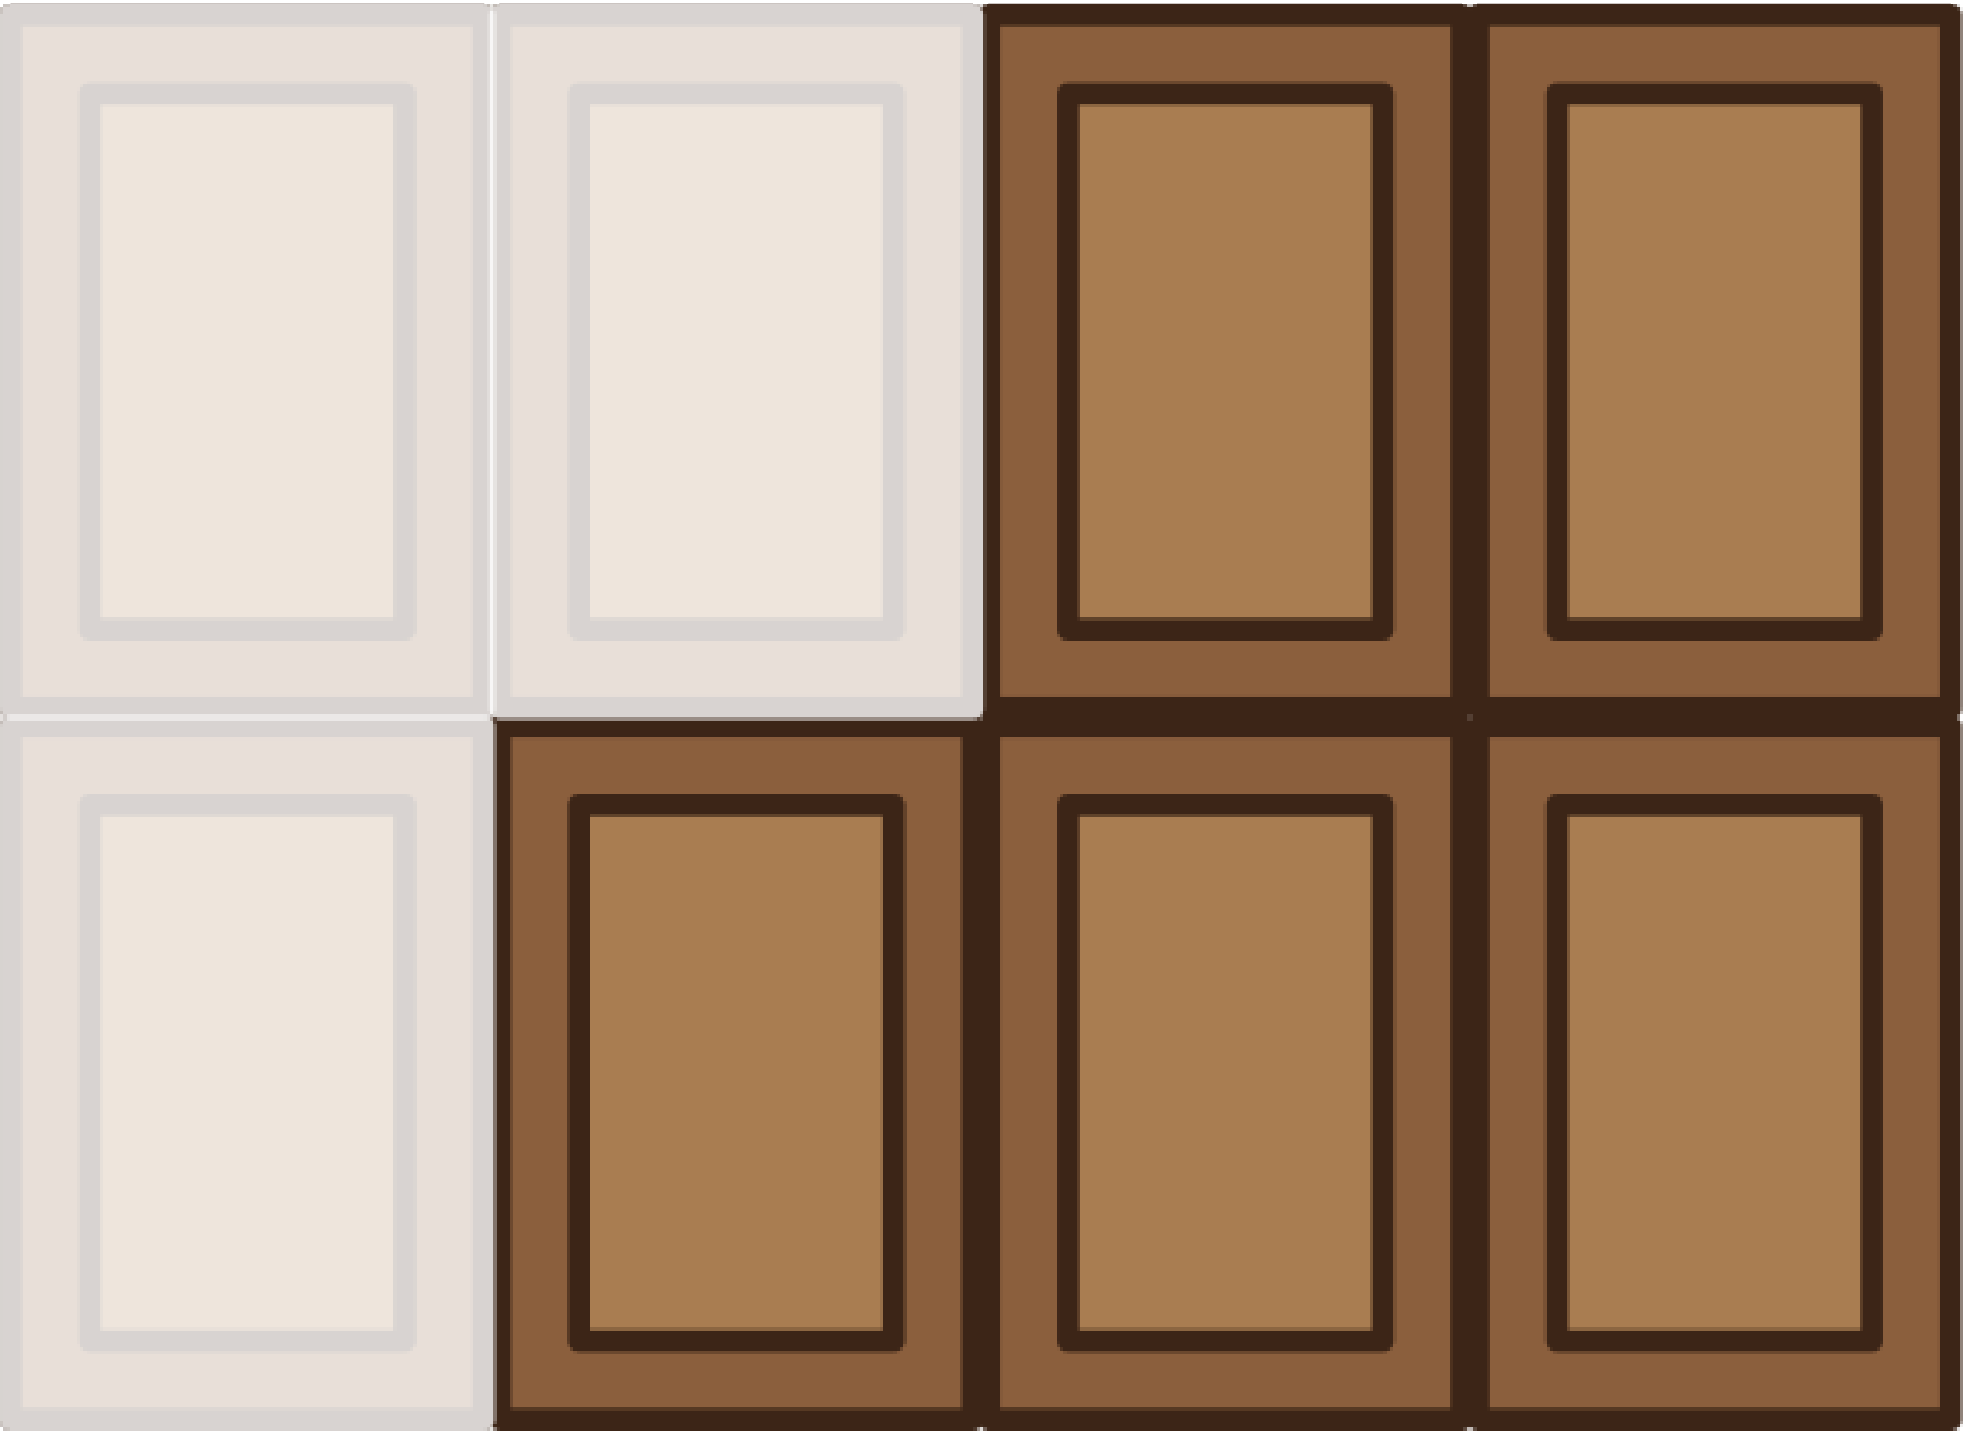
\includegraphics[width=100pt, keepaspectratio]{..//media/cap3/secoes/png/ativ4_fig_b.png} \quad \quad \quad
\begin{tikzpicture}[x=56.25mm,y=56.25mm]
\draw[->] (-0.3,0) -- (1.3,0) ; %edit here for the axis
\foreach \x in  {0,1} % edit here for the vertical lines
\draw[shift={(\x,0)},color=black] (0,3pt) -- (0pt,-3pt) 
node[below] {$\x$};
 
\foreach \x in {3,5}
\draw[shift={(\x/8,0)},color=black] (0,3pt) -- (0pt,-3pt) 
node[below] {$\frac{\x}{8}$};
\end{tikzpicture}   
\end{center}

\item     A unidade é uma maçã. 

\begin{center}

\includegraphics[width=80pt, keepaspectratio]{..//media/cap3/secoes/png/ativ4_fig_c.png} \quad \quad \quad
\begin{tikzpicture}[x=60mm,y=60mm]
\draw[->] (-1/4,0) -- (1+1/4,0) ; %edit here for the axis
\foreach \x in  {0,0.25,...,1}{ % edit here for the vertical lines
\draw[shift={(\x,0)},color=black] (0,3pt) -- (0pt,-3pt);} 
\foreach \x in  {0,1}
\draw[shift={(\x,0)},color=black] (0,3pt) -- (0pt,-3pt) node[below] {$\x$};
\foreach \x in  {1,3}
\draw[shift={(\x/4,0)},color=black] (0,3pt) -- (0pt,-3pt) node[below] {$\frac{\x}{4}$};
\draw[shift={(.5,0)},color=black] (0,3pt) -- (0pt,-3pt) node[below] {$\frac{1}{2}$};
\end{tikzpicture}
\end{center}

  \item     A unidade é um sanduíche de queijo com presunto. 

\begin{center}
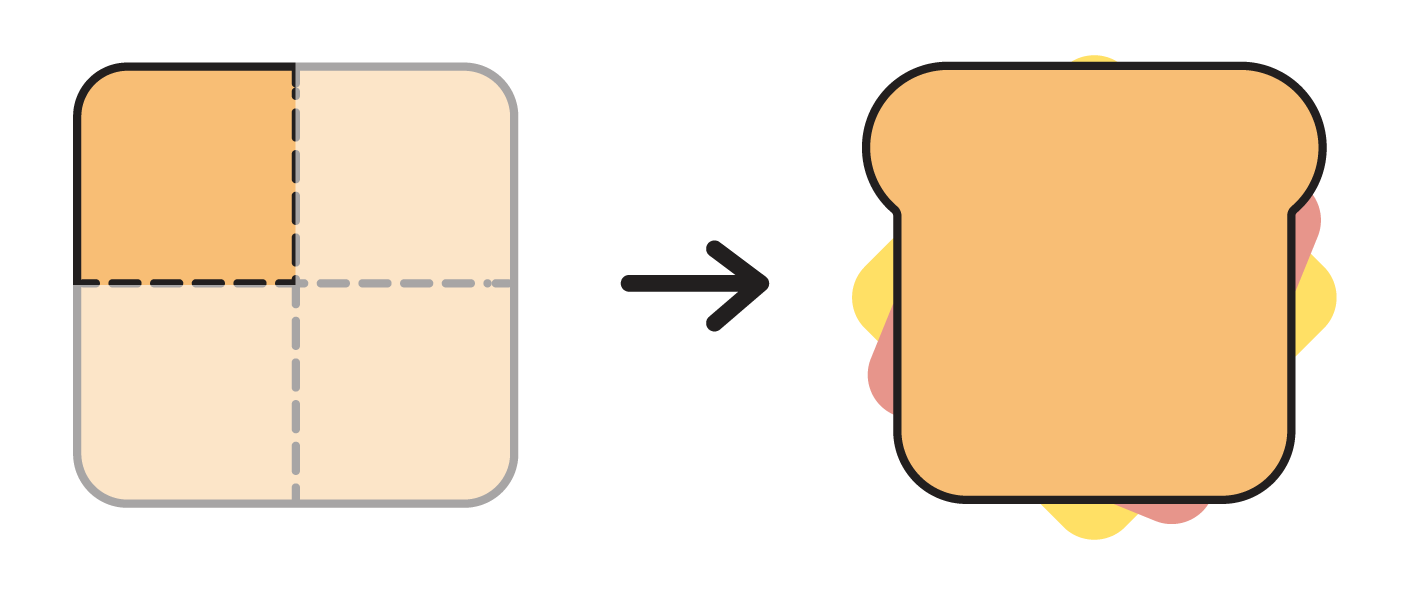
\includegraphics[width=100pt, keepaspectratio]{..//media/cap3/secoes/png/ativ4_fig_d.png} \quad \quad \quad
\begin{tikzpicture}[x=60mm,y=60mm]
\draw[->] (-1/4,0) -- (1+1/4,0) ; %edit here for the axis
\foreach \x in  {0,0.25,...,1}{ % edit here for the vertical lines
\draw[shift={(\x,0)},color=black] (0,3pt) -- (0pt,-3pt);} 
\foreach \x in  {0,1}
\draw[shift={(\x,0)},color=black] (0,3pt) -- (0pt,-3pt) node[below] {$\x$};
\foreach \x in  {1,3}
\draw[shift={(\x/4,0)},color=black] (0,3pt) -- (0pt,-3pt) node[below] {$\frac{\x}{4}$};
\draw[shift={(.5,0)},color=black] (0,3pt) -- (0pt,-3pt) node[below] {$\frac{1}{2}$};
\end{tikzpicture}
\end{center}

\item A unidade é uma torta. 

\begin{center}
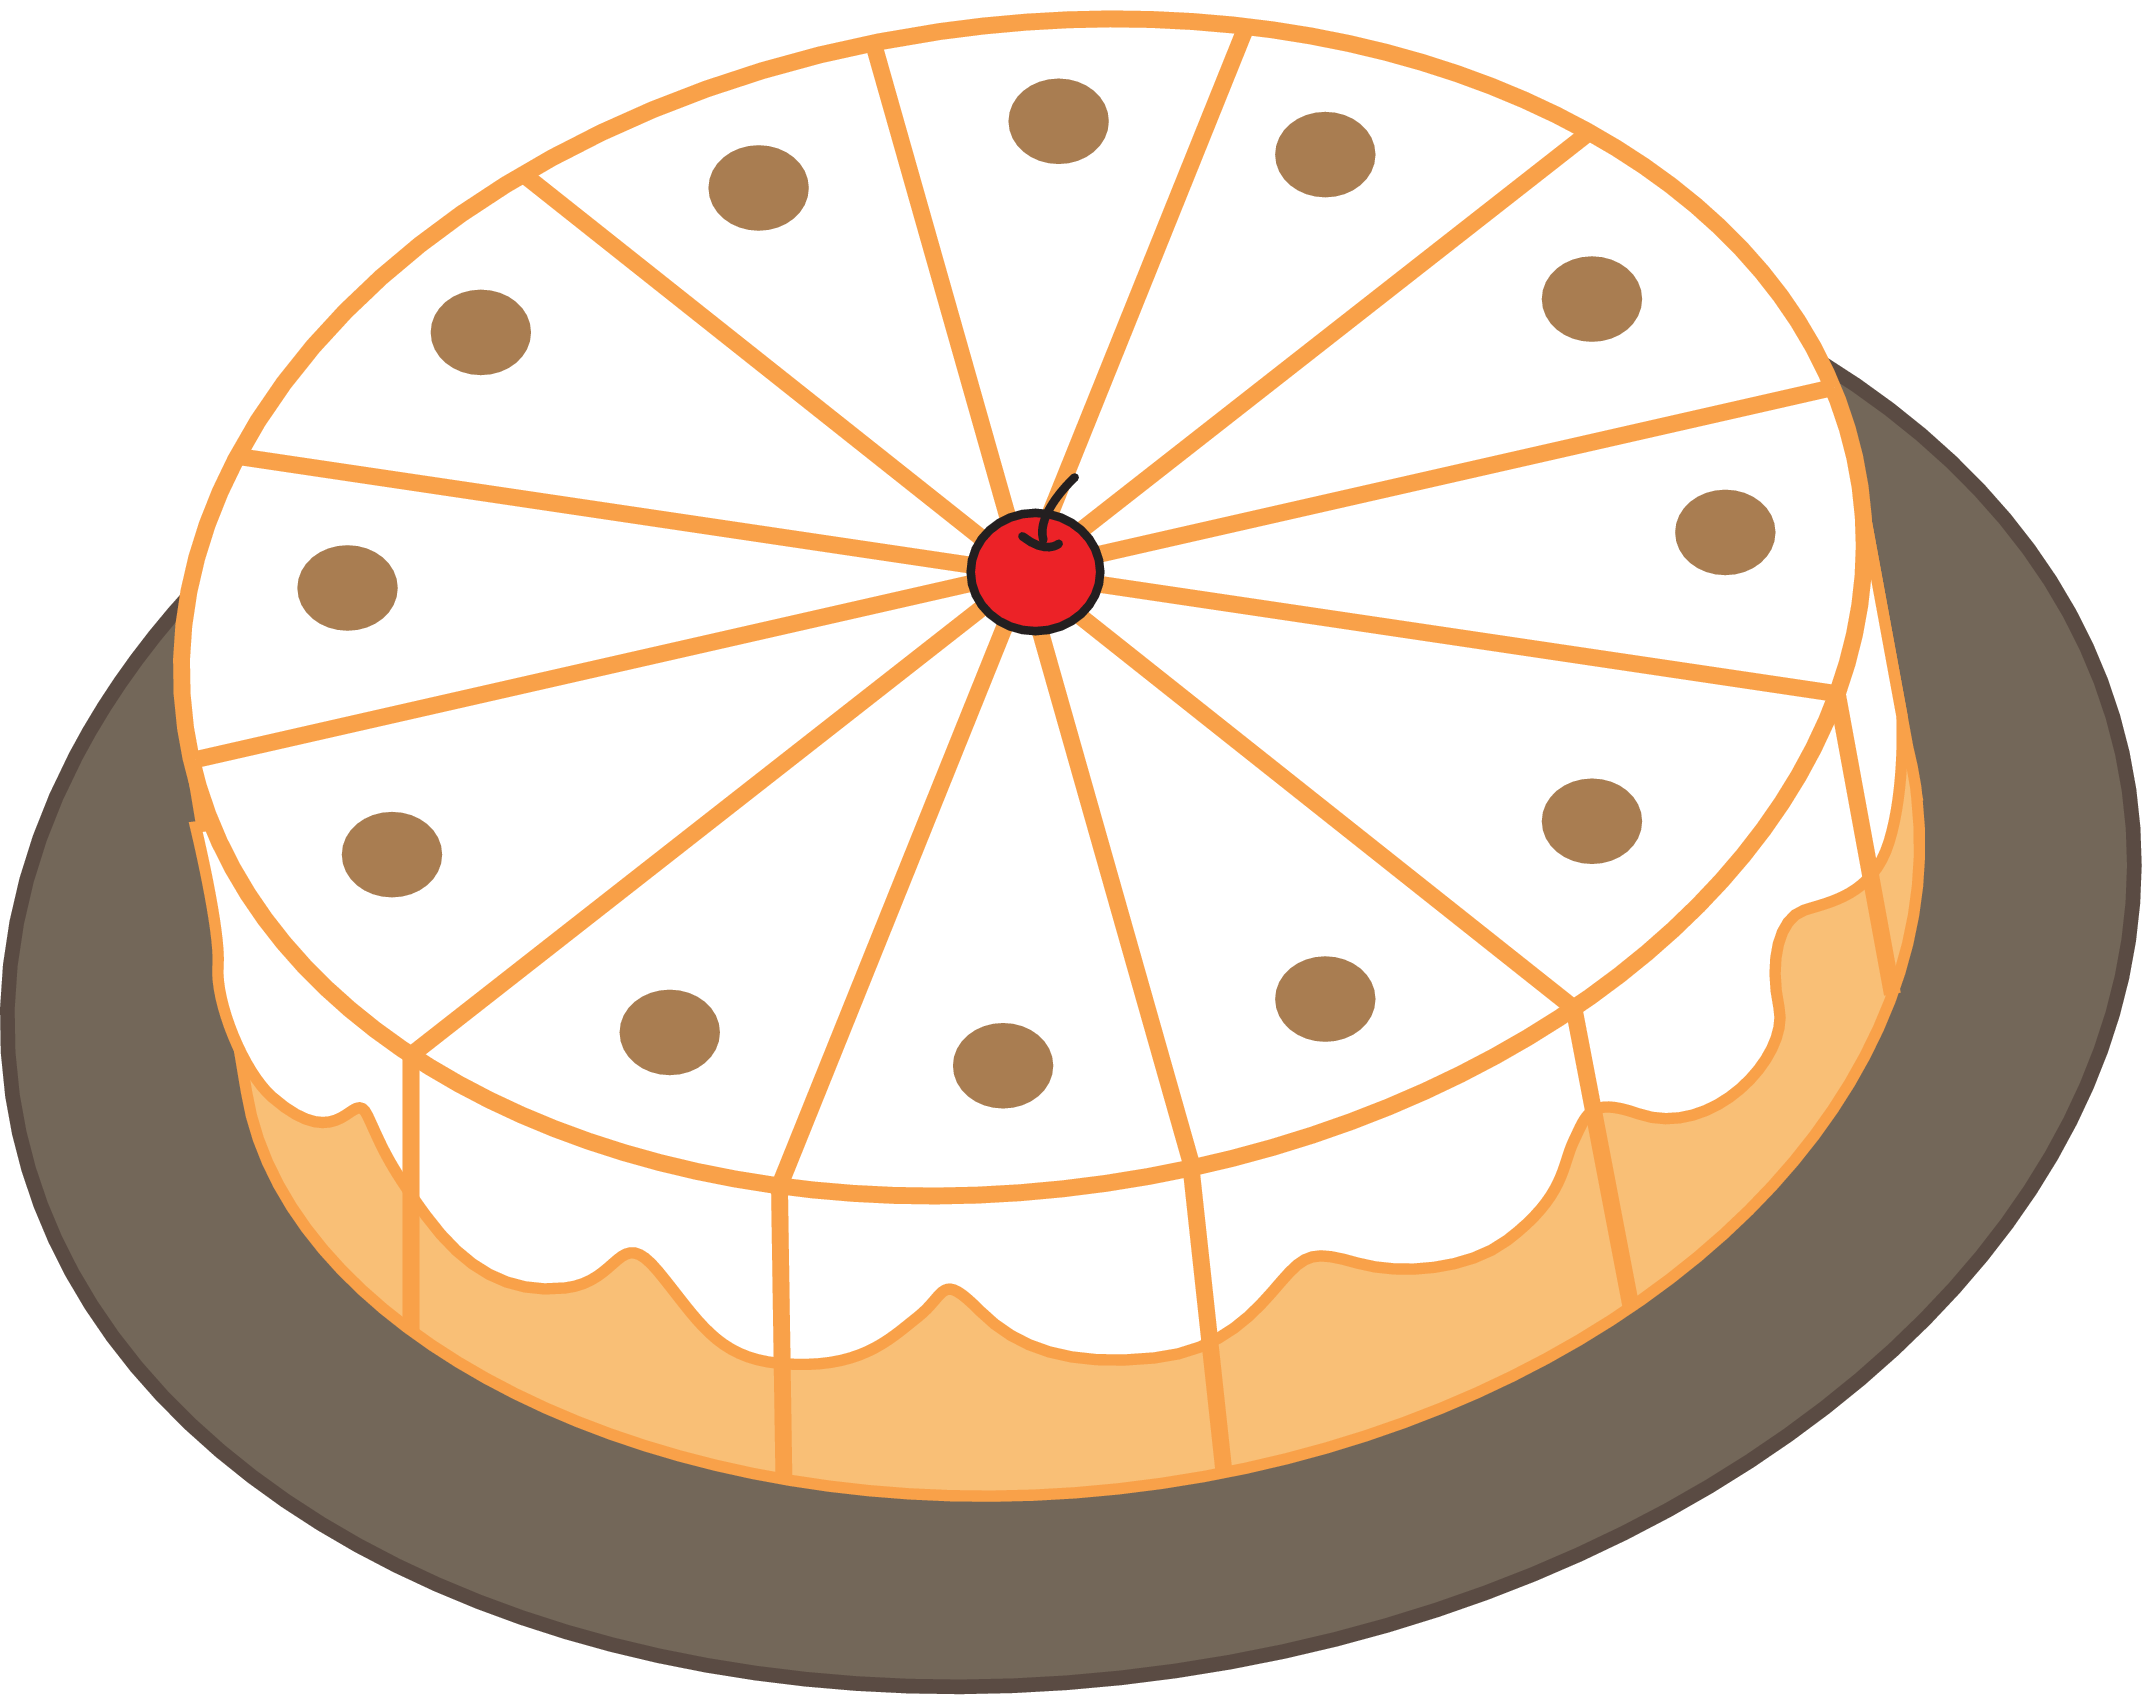
\includegraphics[width=100pt, keepaspectratio]{..//media/cap3/secoes/png/ativ4_fig_e.png} \quad \quad \quad
 \begin{tikzpicture}[x=25.71mm,y=25.71mm]
\draw[->] (-.5,0) -- (3,0) ; %edit here for the axis
\foreach \x in  {0,0.5,...,2.5}{ % edit here for the vertical lines
\draw[shift={(\x,0)},color=black] (0,3pt) -- (0pt,-3pt);} 
\foreach \x in  {0,1,2}
\draw[shift={(\x,0)},color=black] (0,3pt) -- (0pt,-3pt) node[below] {$\x$};
\foreach \x in  {1,3,5}
\draw[shift={(\x/2,0)},color=black] (0,3pt) -- (0pt,-3pt) node[below] {$\frac{\x}{2}$};
\end{tikzpicture}
\end{center}

  \item     A unidade é um biscoito. 

\begin{center}

\includegraphics[width=100pt, keepaspectratio]{..//media/cap3/secoes/png/ativ4_fig_f.png} \quad \quad \quad
\begin{tikzpicture}[x=25.71mm,y=25.71mm]
\draw[->] (-.5,0) -- (3,0) ; %edit here for the axis
\foreach \x in  {0,0.5,...,2.5}{ % edit here for the vertical lines
\draw[shift={(\x,0)},color=black] (0,3pt) -- (0pt,-3pt);} 
\foreach \x in  {0,1,2}
\draw[shift={(\x,0)},color=black] (0,3pt) -- (0pt,-3pt) node[below] {$\x$};
\foreach \x in  {1,3,5}
\draw[shift={(\x/2,0)},color=black] (0,3pt) -- (0pt,-3pt) node[below] {$\frac{\x}{2}$};
\end{tikzpicture}
\end{center}

  \item     A unidade é um copo cheio. 
\end{enumerate} %s

\begin{flushright}
 \begin{tabular}{rcr}

\includegraphics[width=50pt, keepaspectratio]{..//media/cap3/secoes/png/ativ4_fig_g.png}  & \quad\quad\quad\quad&
 \begin{tikzpicture}[x=25.71mm,y=25.71mm]
\draw[->] (-.5,0) -- (3,0) ; %edit here for the axis
\foreach \x in  {0,0.5,...,2.5}{ % edit here for the vertical lines
\draw[shift={(\x,0)},color=black] (0,3pt) -- (0pt,-3pt);} 
\foreach \x in  {0,1,2}
\draw[shift={(\x,0)},color=black] (0,3pt) -- (0pt,-3pt) node[below] {$\x$};
\foreach \x in  {1,3,5}
\draw[shift={(\x/2,0)},color=black] (0,3pt) -- (0pt,-3pt) node[below] {$\frac{\x}{2}$};
\end{tikzpicture}
\end{tabular}
\end{flushright}


\subsection{Atividade}

A faixa a seguir está dividida em 5 partes iguais. 

\begin{center}
 \begin{tikzpicture}[x=56.25mm,y=56.25mm]
\foreach \x in {0,1,2,...,4}{
\draw[fill=common, fill opacity=.3] (\x/5,0) rectangle (\x/5 + 1/5,.1);
\draw[step=.2] (0,0) grid (1,.1);
\draw (0,.1)-- (1,.1);}
 \end{tikzpicture}
\end{center}


\begin{enumerate} [\quad a)] %s
  \item     Considerando a faixa como unidade, escreva na reta numérica a fração correspondente a cada uma das regiões coloridas de vermelho.


\begin{center}
\begin{tikzpicture}[x=56.25mm,y=56.25mm]
\foreach \x in {1,2,...,5}{
\fill[fill=common, fill opacity=.3, shift={(0,-\x*.15)}] (\x/5,0) rectangle (1,.1);
\draw[fill=attention, shift={(0,-\x*.15)}] (0,0) rectangle (\x/5,.1);
\draw[step=.2, shift={(0,-\x*.15)}] (0,0) grid (1,.1);
\draw[shift={(0,-\x*.15)}] (0,.1)-- (1,.1);}
 
\begin{scope}[shift={(0,-.9)}]
\draw[->] (-0.1,0) -- (1.1,0) ; %edit here for the axis
\foreach \x in  {0,1} % edit here for the vertical lines
\draw[shift={(\x,0)},color=black] (0,3pt) -- (0pt,-3pt) node[below] {$\x$};
 
\foreach \x in  {.2,.4,.6,.8} % edit here for the vertical lines
\draw[shift={(\x,0)},color=black] (0,3pt) -- (0pt,-3pt) node[below] {{\Large $\frac{\square}{\square}$}};
\end{scope}

\end{tikzpicture}   
 \end{center}
 
  \item     Escreva, em linguagem simbólica, a fração correspondente à faixa inteira. De que outra maneira é possível indicar essa quantidade? 

\end{enumerate} %s


\subsection{Atividade}

A professora Julia pediu que os seus alunos, Pedro e Miguel, marcassem $\frac{1}{2}$ na reta numérica traçada em uma fita, como esta que vocês também receberam:

\begin{center}
 \begin{tikzpicture}[x=56.25mm,y=56.25mm]
\draw[fill=common, fill opacity=.3] (0,-.15) rectangle (1.2,.15);
\draw (0,0) -- (1.2,0) ; %edit here for the axis
\draw (1,3pt) -- (1,-3pt) node[below] {1};
\node at (.03,-.05) {0};
\end{tikzpicture} 
\end{center}

Pedro trouxe a seguinte marcação: 
 \begin{tikzpicture}[x=56.25mm,y=56.25mm]
\draw[fill=common, fill opacity=.3] (0,-.15) rectangle (1.2,.15);
\draw (0,0) -- (1.2,0) ; %edit here for the axis
\draw[dashed] (0.6,-.15) -- (.6,.15);
\draw (1,3pt) -- (1,-3pt) node[below] {1};
\node at (.03,-.05) {0};
\node at (.63,-.05) {$\frac{1}{2}$};
\end{tikzpicture}

Miguel trouxe esta:
 \begin{tikzpicture}[x=56.25mm,y=56.25mm]
\draw[fill=common, fill opacity=.3] (0,-.15) rectangle (1.2,.15);
\draw (0,0) -- (1.2,0) ; %edit here for the axis
\draw[dashed] (0.5,-.15) -- (.5,.15);
\draw (1,3pt) -- (1,-3pt) node[below] {1};
\node at (.03,-.05) {0};
\node at (.53,-.05) {$\frac{1}{2}$};
\end{tikzpicture} 

\begin{enumerate} [\quad a)] %s
  \item     É possível ambos estarem corretos? Justifique sua resposta. 
  \item     Faça marcações nessa fita correspondentes a     $\frac{1}{4}$     e a     $\frac{3}{4}$    . Explique como você fez essas marcações.
  \item     Onde deve ser feita a marcação correspondente a     $\frac{4}{4}$    ?
  \item     E a marcação de     $\frac{5}{4}$    ? 
\end{enumerate} %s
  
\subsection{Atividade}

Um caçador de tesouros encontrou o mapa a seguir. Leia as instruções para a localização do tesouro e decida em que local ele deve cavar:

\noindent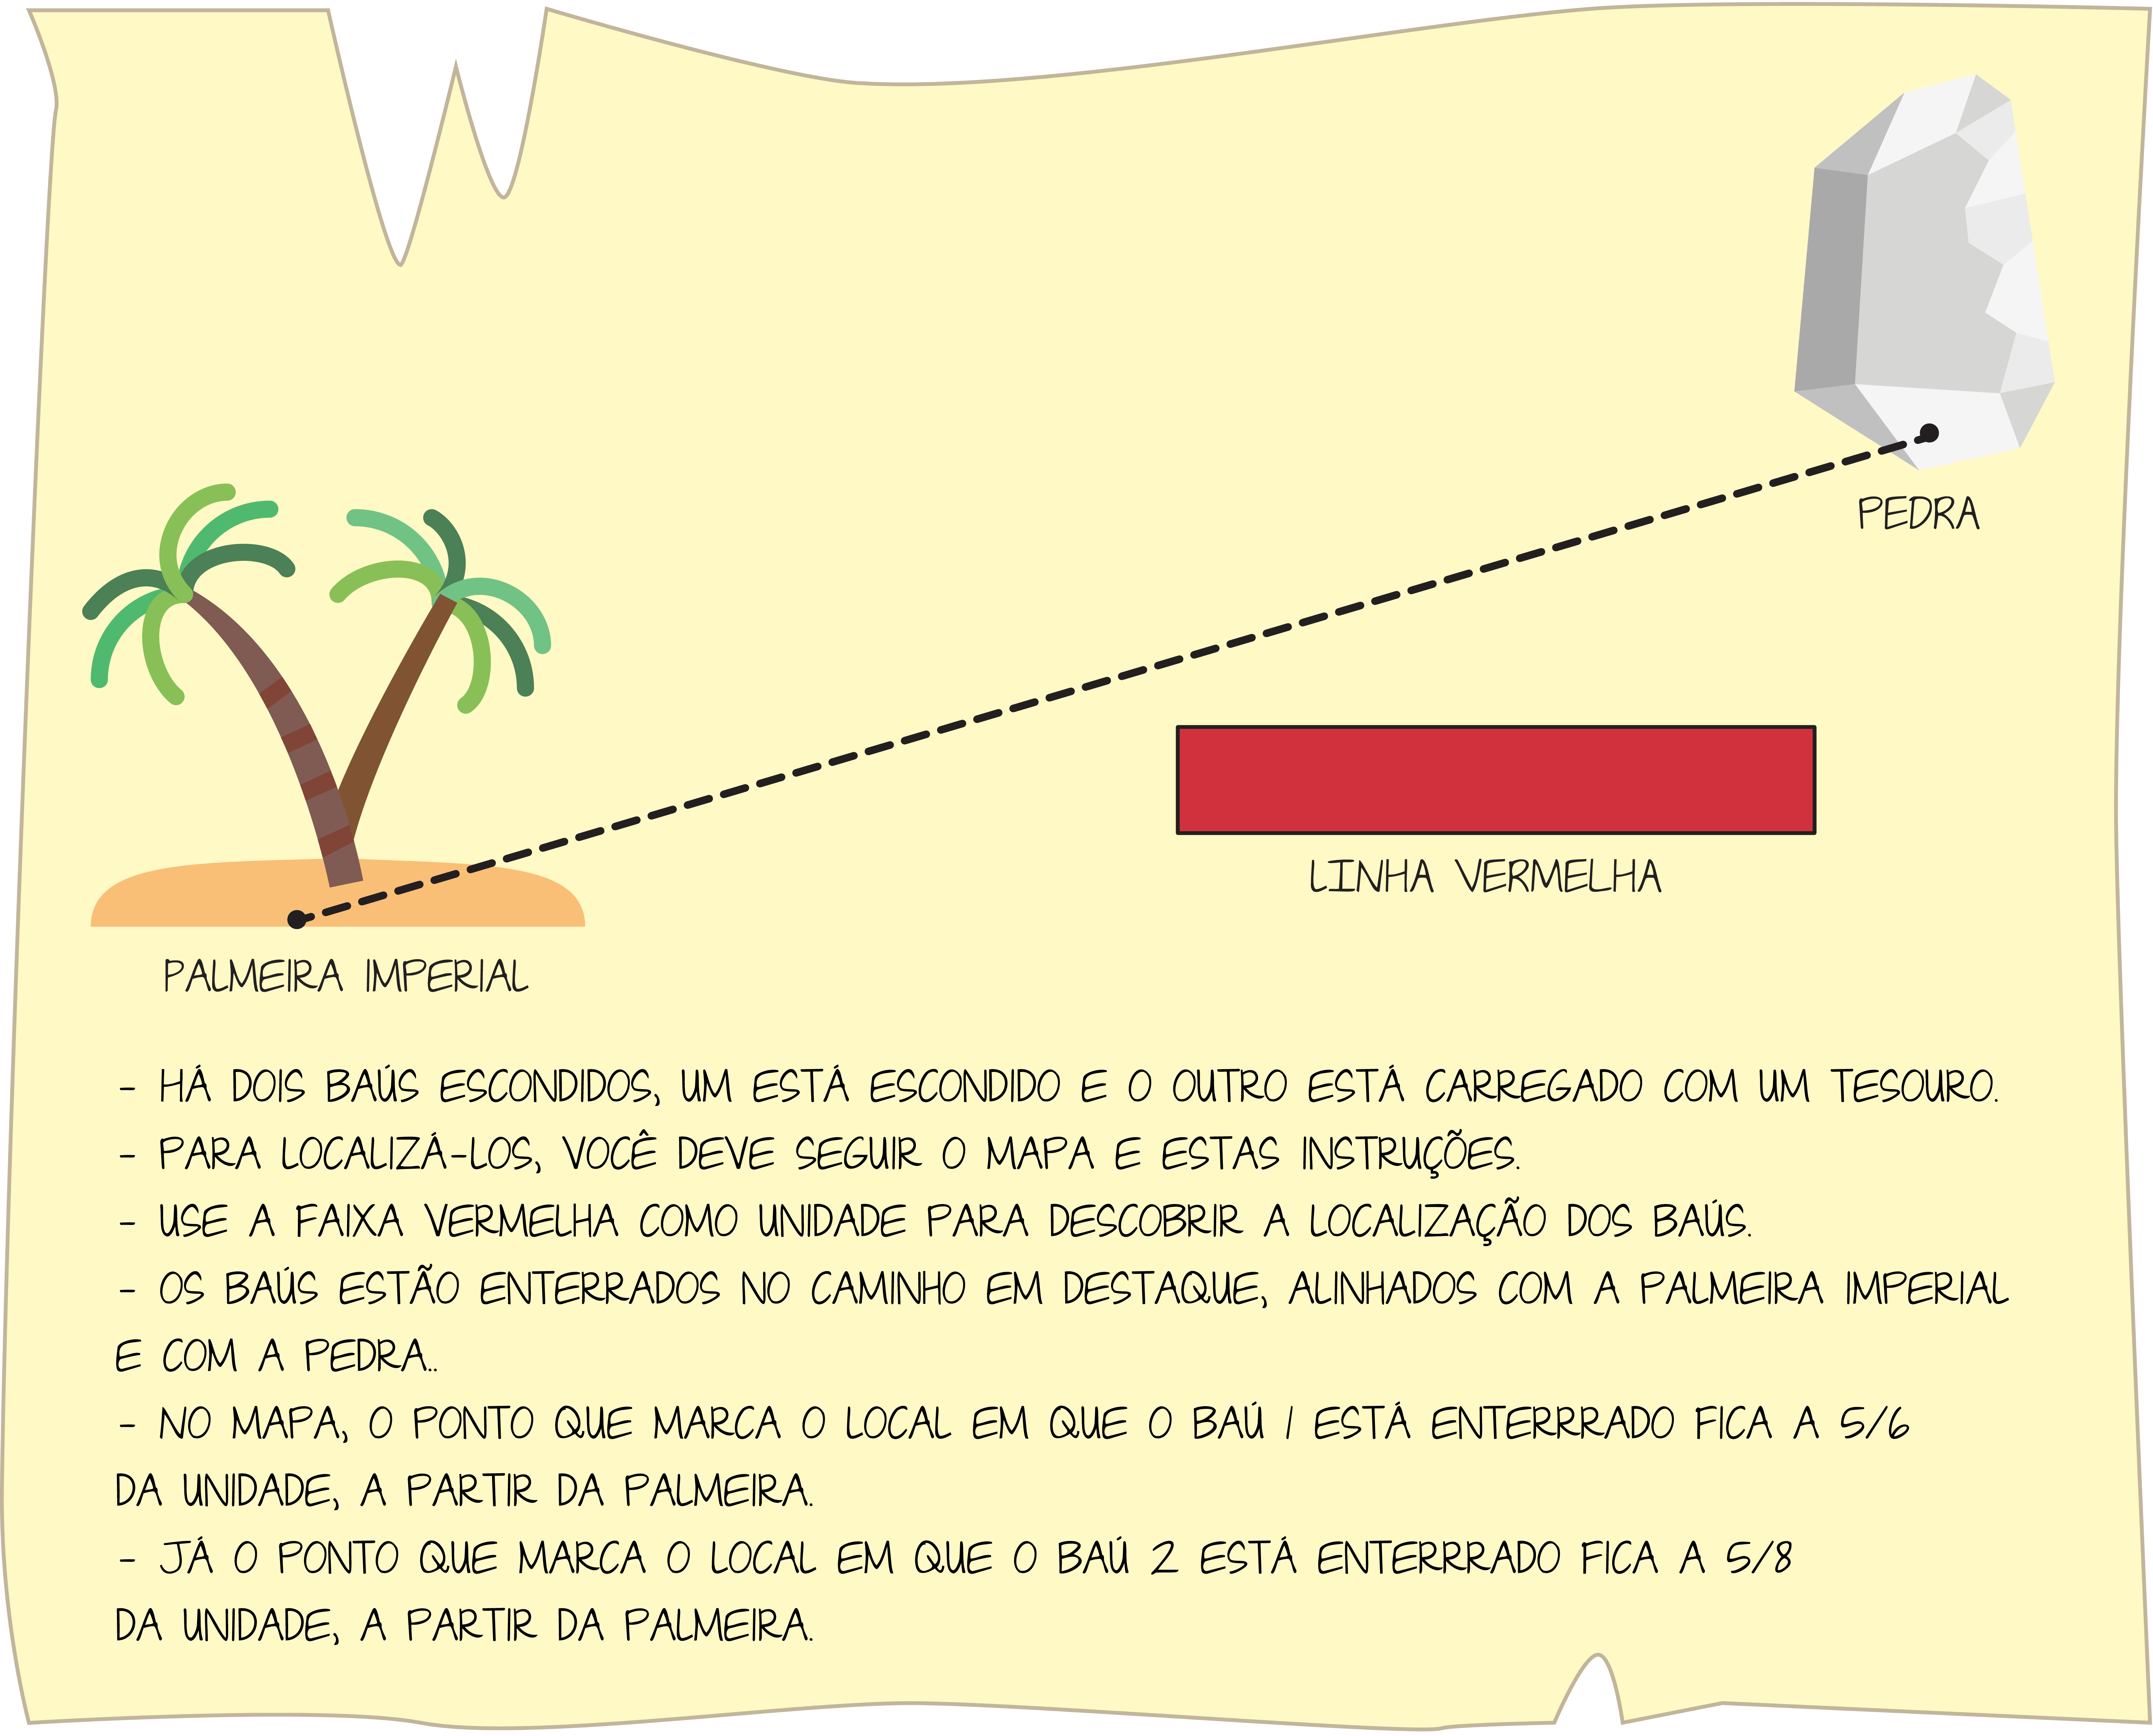
\includegraphics[width=\textwidth, keepaspectratio]{..//media//cap3/secoes/png/ativ7_fig01.png}  

\begin{enumerate}[a)]
 \item Marque, no mapa, as localizações dos baús 1 e 2.
 \item Qual o baú com o tesouro? Explique como chegou à sua conclusão. 
\end{enumerate}

\subsection{Atividade}

Três amigos foram a uma pizzaria e cada um pediu uma pizza média, de três sabores diferentes: João comeu $\frac{3}{4}$ da pizza de calabresa, Maria comeu  $\frac{2}{4}$ da pizza de presunto e Miguel comeu $\frac{3}{5}$ da pizza de Milho. Sabendo que todas as pizzas eram do mesmo tamanho, pergunta-se:
\begin{enumerate} [\quad a)] %s
  \item     Quem comeu mais pizza, João ou Maria? Explique.
  \item     E no caso de João e Miguel, quem comeu mais pizza? Explique.
  \item     Dos três amigos, quem comeu mais pizza? Explique.
  \item     Marque na reta numérica a seguir as frações correspondentes às porções de pizza que cada amigo comeu, e confirme na reta numérica sua resposta em c.
\end{enumerate} %s

\begin{center}
 \begin{tikzpicture}[x=56.25mm,y=56.25mm]
\draw[->] (-0.2,0) -- (1.2,0) ; %edit here for the axis
\foreach \x in {0,1}{ \draw (\x,3pt) -- (\x,-3pt) node[below] {\x};}
\end{tikzpicture}  
\end{center}


\subsection{Atividade}

A imagem a seguir ilustra uma tartaruga percorrendo um caminho em linha reta, do ponto de partida ao de chegada. Observe a posição da tartaruga na imagem e avalie se as afirmações a seguir estão corretas ou não. Em cada item, explique a sua avaliação por escrito.
\begin{enumerate} [\quad a)] %s
  \item     A tartaruga percorreu mais do que a metade do percurso total.
  \item     A tartaruga percorreu mais do que     $\frac{3}{4}$     do percurso total.
  \item     A tartaruga percorreu mais do que     $\frac{3}{8}$     do percurso total.
  \item     A tartaruga percorreu menos do que     $\frac{3}{4}$     do percurso total.
  \item     A tartaruga percorreu menos do que     $\frac{2}{8}$     do percurso total.
  \item     A tartaruga percorreu menos do que     $\frac{2}{3}$     do percurso total.
  \item     A tartaruga percorreu     $\frac{3}{4}$     do percurso total.
  \item     A tartaruga percorreu pelo menos     $\frac{5}{8}$     do percurso total.
  \item     Para alcançar a chegada, a tartaruga precisa percorrer mais do que a metade do caminho.
  \item     Para alcançar a chegada, a tartaruga precisa percorrer menos do que     $\frac{2}{3}$     do caminho.
\end{enumerate} %s

  \noindent
\includegraphics[width=\textwidth, keepaspectratio]{..//media//cap3/secoes/png/ativ9_fig01.png}  

\subsection{Atividade}

Na figura, há várias retas paralelas igualmente espaçadas e outra reta, destacada em vermelho, não paralela às anteriores. Observe que as retas paralelas marcam na reta destacada em vermelho pontos também igualmente espaçados. Dois desses pontos correspondem ao 0 e ao 1. A reta vermelha torna-se uma reta numérica, como ilustra a figura. 

\begin{enumerate} [\quad a)] %s
  \item     Marque, usando os pontos destacados na reta numérica, a fração     $\frac{1}{2}$    . 
  \item     Associe frações a cada um dos pontos destacados na reta numérica. Explique a sua resposta.    \mbox{} \newline      
\begin{center}
 \begin{tikzpicture}[x=56.25mm,y=56.25mm]
 
\begin{scope}
\clip (-.2,-.2) rectangle (.85,.85); 
 
\begin{scope}[ rotate=45]
\foreach \x in {-1.1,-1,...,1.6}{
\draw[common] (\x,0) --+ (45:1); 
\draw[common] (\x,0) --+ (45:-1);}
 
\draw[attention] (-0.2,0) -- (1.2,0) ; %edit here for the axis
\foreach \x in {0,1}{ \draw (\x,3pt) -- (\x,-3pt) node[below] {\x};}
\foreach \x in {0.1,.2,...,.9}{ \draw (\x,3pt) -- (\x,-3pt);}
\end{scope}
\end{scope}
 
\end{tikzpicture}  
\end{center}

Como na figura anterior, há várias retas paralelas igualmente espaçadas e outra reta, destacada em azul, não paralela às anteriores. Observe que as retas paralelas marcam na reta destacada em azul pontos também igualmente espaçados. Dois desses pontos correspondem às frações $\frac{1}{2}$ e $\frac{3}{2}$, como ilustra a figura. 

  \item     Marque, usando os pontos destacados na reta numérica, os pontos correspondentes ao 0 e ao 1
  \item     Marque, nesta mesma reta numérica, as frações     $\frac{3}{4}$     e     $\frac{5}{4}$    .
\begin{center}
  \begin{tikzpicture}[x=56.25mm,y=56.25mm]
 
\begin{scope}
\clip (-.2,-.2) rectangle (.85,.85); 
 
\begin{scope}[ rotate=45]
\foreach \x in {-1.1,-1,...,1.6}{
\draw[common] (\x,0) --+ (135:1); 
\draw[common] (\x,0) --+ (135:-1);}
 
\draw[blue] (-0.2,0) -- (1.2,0) ; %edit here for the axis
\foreach \x in {0,0.1,.2,...,.9}{ \draw (\x,3pt) -- (\x,-3pt);}
\fill[common] (.2,0) circle (3pt) node[below, black] {$\frac{1}{2}$};
\fill[common] (.6,0) circle (3pt) node[below, black] {$\frac{3}{2}$};
\end{scope}
\end{scope}
 
\end{tikzpicture}
\end{center}

\end{enumerate} %s

\section{ORGANIZANDO AS IDEIAS }


Frações na reta numérica

Já é conhecido que os números naturais podem ser representados por pontos em uma reta. 
Para isso, é preciso começar escolhendo dois pontos que vão corresponder ao 0 e ao 1 e, a partir deles, são marcados os pontos que corresponderão aos demais números naturais.

\begin{center}
 \begin{tikzpicture}[x=18mm,y=18mm]
\draw[very thick, attention] (0,0) -- (1,0); 
\node[above] at (.5,0) {unidade};
\draw[->] (-0.5,0) -- (7.5,0) ; %edit here for the axis
\foreach \x in {0,1}{ \draw (\x,3pt) -- (\x,-3pt) node[below] {\x};}
\foreach \x in {0,1}{ \fill[common] (\x,0) circle (3pt);}
 
\end{tikzpicture}   
\end{center}
\vspace{.2cm}

\begin{center}
\begin{tikzpicture}[x=18mm,y=18mm]
 
\begin{scope}[shift={(0,.6)}]
\draw[very thick, attention] (0,0) -- (2,0);% segmento superior
\node[above] at (1,0) {2 unidades};
\foreach \x in {0,1,2}{ \draw (\x,3pt) -- (\x,-3pt);}% marcas verticais
\foreach \x in {0,2} \draw[very thick, ->] (\x,-.1) -- (\x,-.5); 
\end{scope}
 
\draw[->] (-0.5,0) -- (7.5,0) ; %reta anterior
\draw[very thick, attention] (0,0) -- (1,0); 
\foreach \x in {0,1,2}{ \draw (\x,3pt) -- (\x,-3pt) node[below] {\x};}
 
\foreach \x in {0,1,2}{ \fill[common] (\x,0) circle (3pt);}
 
\end{tikzpicture}   
 \end{center}
\vspace{.2cm}

\begin{center} 
\begin{tikzpicture}[x=18mm,y=18mm]
 
\begin{scope}[shift={(0,.6)}]
\draw[very thick, attention] (0,0) -- (7,0);% segmento superior
\node[above] at (3.5,0) {7 unidades};
\foreach \x in {0,1,...,7}{ \draw (\x,3pt) -- (\x,-3pt);}% marcas verticais
\foreach \x in {0,7} \draw[very thick, ->] (\x,-.1) -- (\x,-.5); 
\end{scope}
 
\draw[->] (-0.5,0) -- (7.5,0) ; %reta anterior
\draw[very thick, attention] (0,0) -- (1,0); 
\foreach \x in {0,1,7}{ \draw (\x,3pt) -- (\x,-3pt) node[below] {\x};}
 
\foreach \x in {0,1,7}{ \fill[common] (\x,0) circle (3pt);}
 
\end{tikzpicture}   
\end{center}

As frações também podem ser associadas a pontos na reta numérica. Para isso, é preciso identificar o segmento unitário, aquele cujos extremos são os pontos correspondentes ao 0 e ao 1. Esse segmento representa a unidade.
\begin{center}
\begin{tikzpicture}[x=18mm,y=18mm]
\draw[->] (-0.5,0) -- (7.5,0) ; %edit here for the axis
\foreach \x in {0,1}{ \draw (\x,3pt) -- (\x,-3pt) node[below] {\x};}
\draw[very thick, attention] (0,0) -- (1,0);
\foreach \x in {0,1}{ \fill[common] (\x,0) circle (3pt);}
\end{tikzpicture}   
\end{center}

Dividindo a unidade em partes iguais,  cada uma das partes identifica uma fração da unidade na reta numérica.
Por exemplo, a divisão da unidade em 3 partes iguais identifica terços. O ponto correspondente a $\frac{1}{3}$  é a extremidade do segmento que, a partir do 0, identifica o primeiro terço da unidade. 

\begin{center}
\begin{tikzpicture}[x=18mm,y=18mm]
 
\begin{scope}[shift={(0,.6)}]
\draw[very thick, attention] (0,0) -- (1/3,0);% segmento superior
\node[above] at (1/3,0) {$\frac{1}{3}$ da unidade};
\foreach \x in {0,1/3}{ \draw (\x,3pt) -- (\x,-3pt);}% marcas verticais
\foreach \x in {0,1/3} \draw[very thick, ->] (\x,-.1) -- (\x,-.5); 
\end{scope}
 
\draw[->] (-0.5,0) -- (3.5,0) ; %reta anterior
\draw[very thick, attention] (0,0) -- (1,0); 
\foreach \x in {0,1,...,3}{ \draw (\x,3pt) -- (\x,-3pt) node[below] {\x};}
 
\draw (2/3,3pt) -- (2/3,-3pt);
\node[below] at (1/3,0) {$\dfrac{1}{3}$};
\foreach \x in {0,1}{ \fill[common] (\x,0) circle (3pt);}
\fill[common] (1/3,0) circle (2pt);
\end{tikzpicture}
\end{center}


A partir dele, por justaposições desse segmento, são identificados na reta numérica os pontos correspondentes a $\frac{2}{3}$,$\frac{3}{3}$,$\frac{4}{3}$, e assim por diante. 



\begin{center}
\begin{tikzpicture}[x=18mm,y=18mm]
 
\begin{scope}[shift={(0,.6)}]
\draw[very thick, attention] (0,0) -- (2/3,0);% segmento superior
\node[above] at (1/3,0) {$\frac{2}{3}$ da unidade};
\foreach \x in {0,1/3, 2/3}{ \draw (\x,3pt) -- (\x,-3pt);}% marcas verticais
\foreach \x in {0,2/3} \draw[very thick, ->] (\x,-.1) -- (\x,-.5); 
\end{scope}
 
\draw[->] (-0.5,0) -- (3.5,0) ; %reta anterior
\draw[very thick, attention] (0,0) -- (1,0); 
\foreach \x in {0,1,...,3}{ \draw (\x,3pt) -- (\x,-3pt) node[below] {\x};}
 
\draw (2/3,3pt) -- (2/3,-3pt);
\node[below] at (1/3,0) {$\dfrac{1}{3}$};
\node[below] at (2/3,0) {$\dfrac{2}{3}$};
\foreach \x in {0,1}{ \fill[common] (\x,0) circle (3pt);}
\fill[common] (1/3,0) circle (2pt);
\fill[common] (2/3,0) circle (2pt);
\end{tikzpicture}   
\vspace{.2cm}

\begin{tikzpicture}[x=18mm,y=18mm]
\draw[->] (-0.5,0) -- (3.5,0) ; %reta anterior
\draw[very thick, attention] (0,0) -- (1,0); 
\foreach \x in {0,1,...,3}{ \draw (\x,3pt) -- (\x,-3pt);
\node[above] at (\x,3pt) {\x};}
 
\foreach \x in {0,3,...,9}{ \fill[common] (\x/3,0) circle (3pt);
\node[below] at (\x/3,0) {$\dfrac{\x}{3}$};}
 
\foreach \x in {1,2,4,5,7,8,10}{ \fill[common] (\x/3,0) circle (2pt);
\node[below] at (\x/3,0) {$\dfrac{\x}{3}$};}
 
\end{tikzpicture}   
\end{center}

A representação dos números na reta numérica ajuda a perceber que os pontos correspondentes a algumas frações  são os mesmos que os correspondentes a alguns números naturais. Por exemplo, $\frac{3}{3}$ é igual a 1. 

\begin{center}
\begin{tabular}{cc}
\noindent\includegraphics[width=100pt, keepaspectratio]{..//media//cap3/secoes/png/orgideias_fig_a.png}  &
\noindent\includegraphics[width=100pt, keepaspectratio]{..//media//cap3/secoes/png/orgideias_fig_b.png} \\
\begin{tikzpicture}[x=18mm,y=18mm]
 
\draw[->] (-0.5,0) -- (3.5,0) ; %reta anterior
\draw[very thick, attention] (0,0) -- (1,0); 
\foreach \x in {0,1,...,3}{ \draw (\x,3pt) -- (\x,-3pt);
\node[above] at (\x,3pt) {\x};}
 
\draw (1/3,3pt) -- (1/3,-3pt);
\draw (2/3,3pt) -- (2/3,-3pt);
\node[below] at (1/3,0) {$\dfrac{1}{3}$};
\node[below] at (2/3,0) {$\dfrac{2}{3}$};
%\foreach \x in {0,1/3,2/3,1}{ \fill[common] (\x,0) circle (3pt);}
 
\end{tikzpicture}   &
\begin{tikzpicture}[x=18mm,y=18mm]
 
\draw[->] (-0.5,0) -- (3.5,0) ; %reta anterior
\draw[very thick, attention] (0,0) -- (1,0); 
\foreach \x in {0,1,...,3}{ \draw (\x,3pt) -- (\x,-3pt);
\node[above] at (\x,3pt) {\x};}
 
\draw (1/3,3pt) -- (1/3,-3pt);
\draw (2/3,3pt) -- (2/3,-3pt);
% \node[below] at (1/3,0) {$\dfrac{1}{3}$};
% \node[below] at (2/3,0) {$\dfrac{2}{3}$};
\node[below] at (3/3,0) {$\dfrac{3}{3}$};
%\foreach \x in {0,1/3,2/3,1}{ \fill[common] (\x,0) circle (3pt);}
\end{tikzpicture}   
\end{tabular}
\end{center}

Já $\frac{6}{3}$ é igual a 2. 

\begin{center}
\begin{tabular}{cc}
\includegraphics[width=200pt, keepaspectratio]{..//media//cap3/secoes/png/orgideias_fig_a_2.png} & 
\includegraphics[width=110pt, keepaspectratio]{..//media//cap3/secoes/png/orgideias_fig_b_2.png} \\
\begin{tikzpicture}[x=18mm,y=18mm]
 
\draw[->] (-0.5,0) -- (3.5,0) ; %reta anterior
\draw[very thick, attention] (0,0) -- (1,0); 
\foreach \x in {0,1,...,3}{ \draw (\x,3pt) -- (\x,-3pt);
\node[above] at (\x,3pt) {\x};}
 
\foreach \x in {1,...,5}{\draw (\x/3,3pt) -- (\x/3,-3pt);
\node[below] at (\x/3,0) {$\dfrac{\x}{3}$};}
 
\end{tikzpicture}     &
\begin{tikzpicture}[x=18mm,y=18mm]
 
\draw[->] (-0.5,0) -- (3.5,0) ; %reta anterior
\draw[very thick, attention] (0,0) -- (1,0); 
\foreach \x in {0,1,...,3}{ \draw (\x,3pt) -- (\x,-3pt);
\node[above] at (\x,3pt) {\x};}
 
\draw (1/3,3pt) -- (1/3,-3pt);
\draw (2/3,3pt) -- (2/3,-3pt);
\node[below] at (6/3,0) {$\dfrac{6}{3}$};
\end{tikzpicture}    
\end{tabular}
\end{center}




E $\frac{12}{3}$, é igual a que número natural? $\frac{12}{3}=$

Para identificar na reta numérica os pontos correspondentes às frações $\frac{1}{4}$, $\frac{2}{4}$, $\frac{3}{4}$, $\frac{4}{4}$,$\frac{5}{4}$, $\frac{6}{4}$, e assim por diante, o processo é o mesmo:

\begin{center}
 \begin{tikzpicture}[x=18mm,y=18mm]
\draw[->] (-0.5,0) -- (4.75,0) ; %reta anterior
\draw[very thick, attention] (0,0) -- (1,0); 
\foreach \x in {0,1,...,4}{ \draw (\x,3pt) -- (\x,-3pt);
\node[above] at (\x,3pt) {\x};}
 
\foreach \x in {0,1,...,18}{ \fill[common] (\x/4,0) circle (2pt);
\node[below] at (\x/4,0) {$\dfrac{\x}{4}$};}
 
\foreach \x in {0,4,...,16}{ \fill[common] (\x/4,0) circle (3pt);
\node[below] at (\x/4,0) {$\dfrac{\x}{4}$};}
\end{tikzpicture}   
\end{center}

Na reta numérica a seguir estão destacados alguns pontos e as frações correspondentes a eles. Observe e complete as frações em destaque.

\begin{center}
 \begin{tikzpicture}[x=18mm,y=18mm]
\draw[->] (-0.5,0) -- (3.5,0) ; %reta anterior
\draw[very thick, attention] (0,0) -- (1,0); 
\foreach \x in {0,1,...,20}{ \draw (\x/6,3pt) -- (\x/6,-3pt);}
\foreach \x in {0,1,...,3}{ \draw (\x,3pt) -- (\x,-3pt) node[below] {\x};}
 
\foreach \x in {4,15,20}{ \fill[common] (\x/6,0) circle (3pt);
\node[below] at (\x/6,-9pt) {$\dfrac{}{6}$};}
 
\foreach \x in {2,9}{ \node[below] at (\x/6,-3pt) {$\dfrac{\x}{6}$};}
 
\end{tikzpicture}  
\end{center}

A ordem na reta numérica

Na reta numérica, os números são organizados em ordem crescente, a partir do zero no sentido do 1. Assim, o que vale para o 0, o 1, o 2, o, 3, etc. também valerá para as frações: 

\begin{center}
\begin{tikzpicture}[x=36mm,y=36mm]
 
\begin{scope}[shift={(0,150pt)}]
\draw[->] (-0.1,0) -- (3.5,0) ; %reta anterior
\draw[very thick, attention] (0,0) -- (1,0); 
\foreach \x in {0,1,...,3}{ \draw (\x,3pt) -- (\x,-3pt);
\foreach \x in {0,1,...,6}{ \draw (\x/2,3pt) -- (\x/2,-3pt);}
\node[above] at (\x,3pt) {\x};}
\foreach \x in {1,...,6} \node[below, light] at (\x/2 , 0 pt) {$\frac{\x}{2}$};
\end{scope}
 
\begin{scope}[shift={(0,100pt)}]
\draw[->] (-0.1,0) -- (3.5,0) ; %reta anterior
\draw[very thick, attention] (0,0) -- (1,0); 
\foreach \x in {0,1,...,3}{ \draw (\x,3pt) -- (\x,-3pt);
\foreach \x in {0,1,...,17}{ \draw (\x/5,2pt) -- (\x/5,-2pt);}
\node[above] at (\x,3pt) {\x};}
\foreach \x in {1,...,17} \node[below, attention] at (\x/5 , 0 pt) {$\frac{\x}{5}$};
\end{scope}
 
\begin{scope}[shift={(0,50pt)}]
\draw[->] (-0.1,0) -- (3.5,0) ; %reta anterior
\draw[very thick, attention] (0,0) -- (1,0); 
\foreach \x in {0,1,...,3}{ \draw (\x,3pt) -- (\x,-3pt);
\foreach \x in {0,1,...,34}{ \draw (\x/10,1pt) -- (\x/10,-1pt);}
\node[above] at (\x,3pt) {\x};}
\foreach \x in {0,...,34} \node[below, dark] at (\x/10,0) {$\frac{\x}{10}$};
\end{scope}
 
\draw[->] (-0.1,0) -- (3.5,0) ; %reta anterior
\draw[very thick, attention] (0,0) -- (1,0); 
\foreach \x in {0,1,...,3}{ \draw (\x,3pt) -- (\x,-3pt);
\node[above] at (\x,3pt) {\x};}
 
\foreach \x in {0,1,...,34}{ \draw (\x/10,1pt) -- (\x/10,-1pt);}
\foreach \x in {0,1,...,17}{ \draw (\x/5,2pt) -- (\x/5,-2pt);}
\foreach \x in {0,1,...,6}{ \draw (\x/2,3pt) -- (\x/2,-3pt);}
 
\foreach \x in {0,...,34} \node[below, dark] at (\x/10,0) {$\frac{\x}{10}$};
\foreach \x in {1,2,3,4,6,7,8,9,11,12,13,14,16,17} \node[above, attention] at (\x/5 , 3 pt) {$\frac{\x}{5}$};
\foreach \x in {1,3,5} \node[above, light] at (\x/2 , 3 pt) {\large $\frac{\x}{2}$};
 
\end{tikzpicture}   
\end{center}


Na reta numérica, quanto mais distante do 0 estiver o ponto correspondente ao número, maior será o número. 
\begin{center}
\begin{tikzpicture}[x=54mm,y=54mm]
\draw[->] (-0.5,0) -- (1.5,0) ; %reta anterior
\draw[very thick, attention] (0,0) -- (1,0); 
\foreach \x in {0,1}{ \draw (\x,3pt) -- (\x,-3pt);
\node[below] at (\x,0pt) {\x};}
 
% \node[below] at (1/3,0) {$\dfrac{1}{3}$};
% \node[below] at (2/3,0) {$\dfrac{2}{3}$};
%\node[below] at (6/3,0) {$\dfrac{6}{3}$};
\foreach \x in {3,5}{ \fill[common] (4/\x,0) circle (3pt);
\node[below] at (4/\x,0) {$\dfrac{4}{\x}$};}
 
\end{tikzpicture}
\end{center}

$\frac{4}{3}$ é maior do que $\frac{4}{5}$. Ou ainda, $\frac{4}{5}$ é menor do que $\frac{4}{3}$.


O símbolo é usado $<$ para dizer ``menor do que''.

Por exemplo, a frase ``oito é menor do que quinze'' pode ser expressa de modo mais resumido com ``$8<15$''. Já a expressão $\frac{1}{2}<\frac{3}{2}$ indica que ``um meio é menor do que três meios''.

Do mesmo modo, o símbolo $>$ é usado para significar ``maior do que'', portanto, também pode-se escrever $15>8$ para expressar ``quinze é maior do que oito'' ou $\frac{3}{2}>\frac{1}{2}$  para expressar ``três meios é maior do que um meio''
\begin{center}
  \includegraphics[width=300pt, keepaspectratio]{..//media//cap3/secoes/png/orgideias_fig05.png}   
\end{center}
  
\section{MÃO NA MASSA }

\subsection{Atividade}

{\bf Jogo: varal dos números}

O varal de números está disposto na sala de aula, nele já estão posicionados os números $0$ (zero) e $1$ (um), como na figura. Nos cartões preparados para a atividade estão os números: \\
$0$, $1$, $2$, $3$, $\frac{1}{2}$, $\frac{2}{2}$, $\frac{3}{2}$, $\frac{4}{2}$, $\frac{5}{2}$, $\frac{6}{2}$,
$\frac{1}{3}$, $\frac{2}{3}$, $\frac{3}{3}$, $\frac{4}{3}$, $\frac{7}{3}$, $\frac{9}{3}$,
$\frac{1}{4}$, $\frac{2}{4}$, $\frac{3}{4}$, $\frac{4}{4}$, $\frac{5}{4}$, $\frac{6}{4}$, $\frac{8}{4}$, $\frac{10}{4}$, $\frac{11}{4}$, $\frac{12}{4}$,
$\frac{1}{5}$, $\frac{3}{5}$, $\frac{4}{5}$, $\frac{6}{5}$, $\frac{7}{5}$, $\frac{10}{5}$,
$\frac{1}{10}$.

\begin{center}
\includegraphics[width=300pt, keepaspectratio]{..//media//cap3/secoes/png/ativ11_fig01.png} 
\end{center}


O jogo consiste em fixar cartões numerados em varal, reproduzindo uma reta numérica. As regras serão apresentadas pelo seu professor ou professora. Discuta com seus colegas a posição correta de fixação de cada um dos cartões numerados no varal. 

Ao final do jogo, reproduza a forma como os cartões foram posicionados no varal na reta numérica a seguir. Aproveite as marcações já existentes.

\begin{center}
\begin{tikzpicture}[x=34mm,y=34mm]
\draw[->] (-0.1,0) -- (4,0) ; %reta anterior
\foreach \x in {0,.1,...,3.9}{ \draw (\x,3pt) -- (\x,-3pt);}
\end{tikzpicture}
\end{center}

\subsection{Atividade}

Na reta numérica já estão marcados o 0, o 1 e a fração $\frac{1}{2}$. Marque $\frac{3}{2}$, $\frac{3}{4}$, $\frac{5}{4}$, $\frac{8}{4}$, $\frac{10}{4}$, $\frac{1}{8}$, $\frac{7}{8}$, $\frac{10}{8}$ e 2.

\begin{center}
 \begin{tikzpicture}[x=5mm,y=5mm]
	\draw[->]  (-0.5,0) -- (26,0);
	\draw  (0,-3pt) -- (0,3pt);
	\draw  (1.25,-3pt) -- (1.25,3pt);
	\draw  (2.5,-3pt) -- (2.5,3pt);
	\draw  (3.75,-3pt) -- (3.75,3pt);
	\draw  (5,-3pt) -- (5,3pt);
	\draw  (6.25,-3pt) -- (6.25,3pt);
	\draw  (7.5,-3pt) -- (7.5,3pt);
	\draw  (8.75,-3pt) -- (8.75,3pt);
	\draw  (10,-3pt) -- (10,3pt);
	\draw  (11.25,-3pt) -- (11.25,3pt);
	\draw  (12.5,-3pt) -- (12.5,3pt);
	\draw  (13.75,-3pt) -- (13.75,3pt);
	\draw  (15,-3pt) -- (15,3pt);
	\draw  (16.25,-3pt) -- (16.25,3pt);
	\draw  (17.5,-3pt) -- (17.5,3pt);
	\draw  (18.75,-3pt) -- (18.75,3pt);
	\draw  (20,-3pt) -- (20,3pt);
	\draw  (21.25,-3pt) -- (21.25,3pt);
	\draw  (22.5,-3pt) -- (22.5,3pt);
	\draw  (23.75,-3pt) -- (23.75,3pt);
	\draw  (25,-3pt) -- (25,3pt);

	\node[below] at (0,0) {0};
	\node[below] at (5,0) {$\frac{1}{2}$};
	\node[below] at (10,0)  {1};

\end{tikzpicture}
\end{center}

\subsection{Atividade}


Associe, como no exemplo, cada uma das frações à sua representação na reta numérica.   

\noindent\begin{tabular}{m{.09\textwidth}m{.08\textwidth}m{.08\textwidth}m{.08\textwidth}m{.08\textwidth}m{.08\textwidth}m{0.08\textwidth}m{.08\textwidth}m{0.08\textwidth}}
(A) $\frac{1}{2}$ & (B) $\frac{1}{3}$ &  (C) $\frac{1}{4}$  & (D) $\frac{1}{5}$ & (E) $\frac{1}{6}$  & (F) $\frac{1}{7}$  & (G) $\frac{1}{8}$  & (H) $\frac{1}{9}$  & (I) $\frac{1}{10}$
\end{tabular}

\begin{center}
\begin{longtable}{m{.2\textwidth}m{.5\textwidth}}

\centering \begin{tikzpicture}
 \draw (0,0) -- (20,0);
\end{tikzpicture}
 & 
\parbox[t][1cm][c]{8cm}{
\begin{tikzpicture}[x=50mm,y=50mm]
\draw[->] (-0.3,0) -- (1.3,0) ; %reta anterior
\foreach \x in {0,.1,1}{ \draw (\x,3pt) -- (\x,-3pt);}
 \node[below] at (0,0) {0}; 
 \node[below] at (1,0) {1};
 \fill[common] (.1,0) circle (3pt);
\end{tikzpicture}}
\\
 
 \centering \begin{tikzpicture}
 \draw (0,0) -- (20,0);
 \node[above] at (10,0){(A)};
\end{tikzpicture}
 & 
\parbox[t][1cm][c]{8cm}{
\begin{tikzpicture}[x=50mm,y=50mm]
\draw[->] (-0.3,0) -- (1.3,0) ; %reta anterior
\foreach \x in {0,1}{ \draw (\x,3pt) -- (\x,-3pt);}
 \node[below] at (0,0) {0}; 
 \node[below] at (1,0) {1};
 \fill[common] (.5,0) circle (3pt);
\end{tikzpicture}
}\\
 
\centering \begin{tikzpicture}
 \draw (0,0) -- (20,0);
\end{tikzpicture}
  & 
\parbox[t][1cm][c]{8cm}{
\begin{tikzpicture}[x=50mm,y=50mm]
\draw[->] (-0.3,0) -- (1.3,0) ; %reta anterior
\foreach \x in {0,1}{ \draw (\x,3pt) -- (\x,-3pt);}
 \node[below] at (0,0) {0}; 
 \node[below] at (1,0) {1};
 \fill[common] (1/3,0) circle (3pt);
\end{tikzpicture}
}\\
  
\centering \begin{tikzpicture}
 \draw (0,0) -- (20,0);
\end{tikzpicture}
 & 
\parbox[t][1cm][c]{8cm}{
\begin{tikzpicture}[x=50mm,y=50mm]
\draw[->] (-0.3,0) -- (1.3,0) ; %reta anterior
\foreach \x in {0,1}{ \draw (\x,3pt) -- (\x,-3pt);}
 \node[below] at (0,0) {0}; 
 \node[below] at (1,0) {1};
 \fill[common] (1/9,0) circle (3pt);
\end{tikzpicture}
}\\
 
\centering \begin{tikzpicture}
 \draw (0,0) -- (20,0);
\end{tikzpicture}
 & 
\parbox[t][1cm][c]{8cm}{
\begin{tikzpicture}[x=50mm,y=50mm]
\draw[->] (-0.3,0) -- (1.3,0) ; %reta anterior
\foreach \x in {0,1}{ \draw (\x,3pt) -- (\x,-3pt);}
 \node[below] at (0,0) {0}; 
 \node[below] at (1,0) {1};
 \fill[common] (1/7,0) circle (3pt);
\end{tikzpicture}
}\\
 
\centering \begin{tikzpicture}
 \draw (0,0) -- (20,0);
\end{tikzpicture}
 & 
\parbox[t][1cm][c]{8cm}{
\begin{tikzpicture}[x=50mm,y=50mm]
\draw[->] (-0.3,0) -- (1.3,0) ; %reta anterior
\foreach \x in {0,1}{ \draw (\x,3pt) -- (\x,-3pt);}
 \node[below] at (0,0) {0}; 
 \node[below] at (1,0) {1};
 \fill[common] (.25,0) circle (3pt);
\end{tikzpicture}
}\\
 
\centering \begin{tikzpicture}
 \draw (0,0) -- (20,0);
\end{tikzpicture}
 & 
\parbox[t][1cm][c]{8cm}{
\begin{tikzpicture}[x=50mm,y=50mm]
\draw[->] (-0.3,0) -- (1.3,0) ; %reta anterior
\foreach \x in {0,1}{ \draw (\x,3pt) -- (\x,-3pt);}
 \node[below] at (0,0) {0}; 
 \node[below] at (1,0) {1};
 \fill[common] (1/6,0) circle (3pt);
\end{tikzpicture}
}\\
 
\centering \begin{tikzpicture}
 \draw (0,0) -- (20,0);
\end{tikzpicture}
& 
\parbox[t][1cm][c]{8cm}{
\begin{tikzpicture}[x=50mm,y=50mm]
\draw[->] (-0.3,0) -- (1.3,0) ; %reta anterior
\foreach \x in {0,1}{ \draw (\x,3pt) -- (\x,-3pt);}
 \node[below] at (0,0) {0}; 
 \node[below] at (1,0) {1};
 \fill[common] (1/5,0) circle (3pt);
\end{tikzpicture}
}\\
 
\centering \begin{tikzpicture}
 \draw (0,0) -- (20,0);
\end{tikzpicture}
& 
\parbox[t][1cm][c]{8cm}{
\begin{tikzpicture}[x=50mm,y=50mm]
\draw[->] (-0.3,0) -- (1.3,0) ; %reta anterior
\foreach \x in {0,1}{ \draw (\x,3pt) -- (\x,-3pt);}
 \node[below] at (0,0) {0}; 
 \node[below] at (1,0) {1};
 \fill[common] (1/8,0) circle (3pt);
\end{tikzpicture}
}\\
 
\end{longtable}
\end{center}

\subsection{Atividade}

Observando a atividade anterior (Atividade 13), complete as sentenças a seguir com os sinais $>$ (maior) ou $<$ (menor) de modo a torná-las verdadeiras.
\begin{center}
\begin{tabular}{ccccccccc}
 a)  &   $\dfrac{1}{2}$    & \parbox[t][.6cm]{2cm}{ }\quad\quad\quad      &  $\dfrac{1}{5}$ & \quad\quad\quad\quad\quad\quad\quad   &e)  &  $\dfrac{1}{35}$   & \quad\quad\quad      &  $\dfrac{1}{43}$\\
 b)  &  $\dfrac{1}{4}$    & \parbox[t][.6cm]{2cm}{ }      &  $\dfrac{1}{3}$   & & f)  &  $\dfrac{1}{99}$   &       &  $\dfrac{1}{100}$  \\
 c)  &  $\dfrac{1}{10}$   &  \parbox[t][.6cm]{2cm}{ }     &  $\dfrac{1}{20}$  & & g)  &  $\dfrac{1}{5}$    &       &  $\dfrac{1}{50}$  \\
 d)  &  $\dfrac{1}{12}$   & \parbox[t][.6cm]{2cm}{ }      &  $\dfrac{1}{2}$   & & h)  &  $\dfrac{1}{100}$  &       &  $\dfrac{1}{10}$  \\ 
 \end{tabular}
 \end{center}


\subsection{Atividade}

Na reta numérica a seguir estão destacados os pontos correspondentes ao 0, ao 1 e a $\frac{1}{2}$. Os demais pontos correspondem às frações apresentadas a seguir. Associe cada fração ao ponto correspondente.  

\begin{center}
\begin{tikzpicture}[x=.3cm,y=.3cm,]
	\draw[->] (-2,0) -- (47,0);
		
	\fill[common] (0,0) circle (3 pt);		%0
	\fill[common] (10,0) circle (3 pt);
	\fill[common] (15,0) circle (3 pt);
	\fill[common] (20,0) circle (3 pt);
	\fill[common] (25,0) circle (3 pt);
	\fill[common] (30,0) circle (3 pt);
	\fill[common] (32,0) circle (3 pt);
	\fill[common] (36,0) circle (3 pt);
	\fill[common] (40,0) circle (3 pt);
	\fill[common] (44,0) circle (3 pt);
	\fill[common] (45,0) circle (3 pt);

		\node[below]  at (0,-1) {0};			%0
		\node[below]  at (20,-1) {$\frac{1}{2}$};	%1/2
		\node[below]  at (40,-1) {1};			%1

	 	     \tikzstyle{gray_block} = [draw,outer sep=3,inner sep=3,minimum size=1,line width=1, very thick, draw=black!55, top color=white,bottom color=black!20]
	\node [gray_block] at (10.5,5) {$\frac{1}{4}$};   
  	\node [gray_block] at (14.5,5) {$\frac{3}{4}$};
	\node [gray_block] at (18.5,5) {$\frac{4}{5}$};
	\node [gray_block] at (22.5,5) {$\frac{3}{8}$};
	\node [gray_block] at (26.5,5) {$\frac{5}{8}$};
	\node [gray_block] at (30.5,5) {$\frac{9}{8}$};
	\node [gray_block] at (35,5) {$\frac{9}{10}$};
	\node [gray_block] at (40,5) {$\frac{11}{10}$};
\end{tikzpicture}
\end{center}

\subsection{Atividade}


Complete as sentenças a seguir com os sinais $>$ (maior), $<$ (menor) ou $=$ (igual) de modo a torná-las verdadeiras. 

\begin{center}
\begin{tabular}{lccccccccccccc}
 a)  &  $\dfrac{3}{6}$     &   &  $\dfrac{5}{6}$   & \parbox[t][.6cm]{2cm}{ } \quad \quad\quad  & f)  &  $\dfrac{1}{2}$     &   &  $\dfrac{1}{3}$    & \quad \quad\quad  & m)  &  $\dfrac{3}{2}$     &   &  $\dfrac{2}{5}$    \\
 b)  &  $\dfrac{5}{9}$     &   &  $\dfrac{4}{9}$   & \parbox[t][.6cm]{2cm}{ }    & g)  &  $\dfrac{1}{7}$     &   &  $\dfrac{1}{6}$    &   & n)  &  $\dfrac{3}{4}$     &   &  $\dfrac{6}{5}$    \\
 c)  &  $\dfrac{7}{10}$    &   &  $\dfrac{9}{10}$   & \parbox[t][.6cm]{2cm}{ }   & h)  &  $\dfrac{2}{5}$     &   &  $\dfrac{2}{7}$    &   & o)  &  $\dfrac{7}{8}$     &   &  $\dfrac{10}{9}$   \\
 d)  &  $\dfrac{3}{12}$    &   &  $\dfrac{9}{12}$   & \parbox[t][.6cm]{2cm}{ }   & i)  &  $\dfrac{4}{5}$     &   &  $\dfrac{4}{3}$    &   & p)  &  $\dfrac{6}{5}$     &   &  $\dfrac{12}{9}$   \\
 e)  &  $\dfrac{39}{100}$  &   &  $\dfrac{25}{100}$ & \parbox[t][.6cm]{2cm}{ }   & j)  &  $\dfrac{12}{15}$   &   &  $\dfrac{12}{7}$   &   & q)  &  $\dfrac{4}{5}$     &   &  $\dfrac{5}{4}$    \\
     &&                     &    &                  \parbox[t][.6cm]{2cm}{ }    &  l)  &  $\dfrac{22}{80}$   &   &  $\dfrac{22}{90}$  &   & r)  &  $\dfrac{35}{40}$   &   &  $\dfrac{30}{25}$  \\
     &&                      &    &                    &      &  \parbox[t][.6cm]{2cm}{ }                    &   &                   &   &  s)  &  $\dfrac{99}{100}$  &   &  $\dfrac{3}{2}$    \\
\end{tabular} 
 \end{center}
 
\section{QUEBRANDO A CUCA }


\subsection{Atividade}

Você recebeu uma folha com retângulos que têm o mesmo tamanho mas que são coloridos de maneira diferente. Em cada um deles há marcações que representam uma equipartição.  

\begin{enumerate}[a)]
\item Complete os retângulos, ecrevendo em cada um deles a fração representada por cada parte da equipartição, como no exemplo
\begin{center}
\begin{tikzpicture}[scale=.5]
\draw[fill=gray] (0,0) rectangle (60,12);
    \end{tikzpicture}

\begin{tikzpicture}[scale=.5]
\draw[fill=light] (0,0) rectangle (60,12);
\draw (30,0) -- (30,12);
\node at (15,6) {{\small $\frac{1}{2}$}};
\node at (45,6) {{\small $\frac{1}{2}$}};
\end{tikzpicture}
    
   \begin{tikzpicture}[scale=.5]
\draw[fill=pink] (0,0) rectangle (60,12);
\foreach \x in {1,2} \draw (\x*60/3,0) -- (\x*60/3,12);
    \end{tikzpicture}        
    
      \begin{tikzpicture}[scale=.5]
\draw[fill=special] (0,0) rectangle (60,12);
\foreach \x in {1,2,3} \draw (\x*60/4,0) -- (\x*60/4,12);
    \end{tikzpicture}        
    
   \begin{tikzpicture}[scale=.5]
\draw[fill=attention] (0,0) rectangle (60,12);
\foreach \x in {1,...,4} \draw (\x*60/5,0) -- (\x*60/5,12);
    \end{tikzpicture}        
    
   \begin{tikzpicture}[scale=.5]
\draw[fill=common] (0,0) rectangle (60,12);
\foreach \x in {1,...,5} \draw (\x*60/6,0) -- (\x*60/6,12);
    \end{tikzpicture}        
    
    \begin{tikzpicture}[scale=.5]
\draw[fill=CornflowerBlue] (0,0) rectangle (60,12);
\foreach \x in {1,...,6} \draw (\x*60/7,0) -- (\x*60/7,12);
    \end{tikzpicture}        
    
   \begin{tikzpicture}[scale=.5]
\draw[fill=dark] (0,0) rectangle (60,12);
\foreach \x in {1,...,7} \draw (\x*60/8,0) -- (\x*60/8,12);
    \end{tikzpicture}        
    
   \begin{tikzpicture}[scale=.5]
\draw[fill=Fuchsia] (0,0) rectangle (60,12);'
\foreach \x in {1,...,8} \draw (\x*60/9,0) -- (\x*60/9,12);
    \end{tikzpicture}        
    
 \begin{tikzpicture}[scale=.5]   
 \draw[fill=NavyBlue] (0,0) rectangle (60,12);
 \foreach \x in {1,...,9} \draw (\x*60/10,0) -- (\x*60/10,12);
     \end{tikzpicture}        
    
\begin{tikzpicture}[scale=.5]   
    \draw[fill=BlueViolet] (0,0) rectangle (60,12);
\foreach \x in {1,...,15} \draw (\x*60/16,0) -- (\x*60/16,12);
    \end{tikzpicture}        
 \end{center}
\item  Recorte os retângulos coloridos da folha que você recebeu e use-os para representar na reta numérica os seguintes números: 

$0$, $1$, $\frac{1}{2}$, $\frac{1}{3}$, $\frac{1}{4}$, $\frac{3}{4}$, $\frac{3}{5}$, $\frac{5}{6}$, $\frac{7}{6}$, $\frac{6}{7}$,  $\frac{10}{7}$,  $\frac{12}{7}$,  $\frac{10}{8}$,  $\frac{12}{8}$, $\frac{10}{9}$, $\frac{12}{9}$, $\frac{10}{10}$, $\frac{20}{16}$

\begin{center}
 \begin{tikzpicture}[scale=.5]
\draw[->] (-10,0) -- (150,0);
\foreach \x in {0,60} \draw (\x,-6pt) -- (\x,6 pt);
\node at (0,-20pt) {0};
\node at (60,-20pt) {1};
\end{tikzpicture}
\end{center}


\end{enumerate}


\subsection{Atividade}


Na reta numérica a seguir:
\begin{enumerate} [\quad a)] %s
  \item     Marque     $\frac{1}{2}$    . Justifique sua resposta.
  \item     Marque     $\frac{1}{4}$    ,     $\frac{3}{4}$     e     $\frac{5}{4}$    . Explique como raciocinou para fazer essas marcações. 
  
\begin{center}
\begin{tikzpicture}[x=15mm,y=15mm]
\draw[->] (-0.5,0) -- (5.5,0) ; %reta anterior
\foreach \x in {0,2}{ \draw (\x,3pt) -- (\x,-3pt);}
\node[below] at (0,0) {0};
\node[below] at (2,0) {2};
\end{tikzpicture}
\end{center}

Observando a reta numérica com as marcações feitas, compare: 

  \item $\frac{1}{4}$     é maior ou menor do que     $\frac{1}{2}$    ? 
  \item $\frac{3}{4}$ é maior ou menor do que $\frac{1}{2}$    ?
  \item $\frac{5}{4}$  é menor do que 1?
  \item Escreva as frações marcadas na reta em ordem crescente, completando os espaços a seguir:

$$0 < \frac{\square}{\square} < \frac{\square}{\square}< \frac{\square}{\square} < 1 < \frac{\square}{\square}$$

Volte à reta e marque outras três frações que atendam às seguintes condições: 
  \item A primeira deve ser maior do que $3$ e menor do que $4$.
 \item A segunda deve ser maior do que $\frac{7}{2}$.
 \item A terceira deve ser maior do que $\frac{17}{4}$ e menor do que $5$

\end{enumerate} %s




 

\setcounter{chapter}{3}
\chapter{Comparação e Igualdade de Frações }
\setcounter{subsection}{0}
\vspace*{-1.3cm}

\hspace*{-1.3cm}\begin{tabular}{cc}
\includegraphics[width=.48\paperwidth, keepaspectratio]{licao04/quadrinho_01.png} &
\includegraphics[width=.48\paperwidth, keepaspectratio]{licao04/quadrinho_02.png} \\
\includegraphics[width=.48\paperwidth, keepaspectratio]{licao04/quadrinho_03.png} &
\includegraphics[width=.48\paperwidth, keepaspectratio]{licao04/quadrinho_04.png}
         \end{tabular}

%\vspace*{-3cm}

\section{EXPLORANDO O ASSUNTO }

\begin{atividade}{}

A turma de Rita vai fazer um piquenique. A professora comprou pães para a turma preparar sanduíches. Cada colega de Rita preparou um sanduíche e partiu-o em partes iguais. Veja como alguns dos colegas repartiram o seu sanduiche:


\begin{center}
\begin{tabular}{cccc}
\begin{tikzpicture}
\draw[fill=common, fill opacity=.3] (0,0) rectangle (20,20);
\draw (0,0) -- (20,20);
\node[below] at (10,0){(A)};
\end{tikzpicture}
&
\begin{tikzpicture}
\draw[fill=common, fill opacity=.3] (0,0) rectangle (20,20);
\draw (0,20/3) -- (20,20/3);
\draw (0,40/3) -- (20,40/3);
\node[below] at (10,0){(B)};
\end{tikzpicture}
&
\begin{tikzpicture}
\draw[fill=common, fill opacity=.3] (0,0) rectangle (20,20);
\draw (0,0) -- (20,20);
\draw (20,0) -- (0,20);
\node[below] at (10,0){(C)};
\end{tikzpicture}
&
\begin{tikzpicture}
\draw[fill=common, fill opacity=.3] (0,0) rectangle (20,20);
\draw (10,0) -- (10,20);
\draw (0,10) -- (20,10);
\node[below] at (10,0){(D)};
\end{tikzpicture}
\end{tabular}
\end{center}


\begin{enumerate} [\quad a)] %s
  \item     Nessas repartições, que fração do sanduíche pode representar cada uma das partes em que o sanduíche foi repartido?
  \item     Em quais dessas repartições é possível comer metade do sanduíche repartido sem parti-lo ainda mais? Justifique sua resposta!
  \item     Para cada uma das repartições que você deu como resposta no item b), expresse, por meio de frações, a metade do sanduíche.
\end{enumerate} %s
\end{atividade}

\begin{atividade}[label=chap4-ativ2]{}
\phantomsection

O \textit{retângulo maior} na folha que você recebeu está dividido em 10 retângulos menores, três deles estão coloridos. Dobre a folha como ilustrado na primeira coluna - ``Como dobrar''. As dobras formam novos \textit{retângulos menores}. Preencha a tabela a seguir, uma linha de cada vez, considerando as dobras feitas.
\clearpage

 \begin{longtable}{|m{.30\textwidth}|m{.16\textwidth}|m{.16\textwidth}|m{.31\textwidth}|}
    \hline
      Como dobrar  &  Quantidade total de retângulos menores & Quantidade de retângulos menores pintados  &   Fração do retângulo maior do encarte que está pintada  \\
    \hline \hline
    \endhead
    \includegraphics[width=110pt, keepaspectratio]{licao04/ativ2_fig01.png}      & $$10$$ & $$3$$&  $$\dfrac{3}{10}$$   \\
    \hline
     \includegraphics[width=110pt, keepaspectratio]{licao04/ativ2_fig02.png}                                                                              & &  &  \\
    \hline
     \includegraphics[width=110pt, keepaspectratio]{licao04/ativ2_fig03.png}     &  &   &  \\
    \hline
     \includegraphics[width=110pt, keepaspectratio]{licao04/ativ2_fig04.png} & &&\\
    \hline
     \includegraphics[width=110pt, keepaspectratio]{licao04/ativ2_fig05.png}  &                                     &                                  &                                                   \\
    \hline
     \includegraphics[width=110pt, keepaspectratio]{licao04/ativ2_fig06.png} &                                     &                                  &                                                   \\
    \hline
  \end{longtable}
\end{atividade}
\clearpage

\begin{refletindo*}
  Na \hyperref[chap4-ativ2]{atividade 2}, o retângulo maior está inicialmente dividido em dez retângulos menores iguais com três deles pintados de amarelo. Então a ``Fração do retângulo maior que está pintada de amarelo é $\frac{3}{10}$.''

\begin{center}
  \includegraphics[width=.45\textwidth, keepaspectratio]{licao04/dobradura-geogebra-10x1.png}\quad \includegraphics[width=.45\textwidth, keepaspectratio]{licao04/dobradura-geogebra-10x2.png}
\end{center}

  Depois de dobrar a folha em duas partes iguais, o número total de retângulos menores passa a ser 20, o dobro da quantidade inicial. A  quantidade total de retângulos menores pintados passa a ser 6. Dessa forma a ``Fração do retângulo maior que está pintada de amarelo é $\frac{6}{20}$.''

Como a parte do retângulo pintada de amarelo não mudou quando a folha foi dobrada,  então $\frac{3}{10}$ do retângulo maior é igual a  $\frac{6}{20}$ do retângulo maior. Essas frações representam a mesma quantidade:

$$\dfrac{3}{10} = \dfrac{6}{20} = \dfrac{2 \times 3}{2 \times 10},$$
sendo 2 é o número de partes em que a folha foi dobrada.

Da mesma forma, depois de dobrar a folha em 4 partes iguais, o número total de retângulos menores passa a ser 40, quatro vezes a quantidade inicial. A quantidade total de retângulos menores pintados também fica multiplicada por 4 e passa a ser 12. Dessa forma, a  ``Fração do retângulo maior que está pintada de amarelo é $\frac{12}{40}$.''

$$\dfrac{3}{10} = \dfrac{12}{40} = \dfrac{4 \times 3}{4 \times 10},$$
sendo 4 é o número de partes em a folha foi dobrada.

\begin{center}
\includegraphics[width=.55\textwidth, keepaspectratio]{licao04/dobradura-geogebra-10x4.png}
\end{center}

Se quiser, use este aplicativo (\url{https://www.geogebra.org/m/fkb5vpze}) no computador, tablet ou no celular para rever as imagens e ajudar na contagem.

Agora é a sua vez:

\begin{center}
  \fbox{\includegraphics[width=.6\textwidth, keepaspectratio]{licao04/dobradura-geogebra-10x3.png}}
\end{center}

Depois de dobrar a folha em três parte, o número total de retângulos menores passa a ser $\underline{\phantom{1000}}$, o $\underline{\phantom{1000}}$ da quantidade inicial. A  quantidade total de retângulos menores pintados passa a ser $\underline{\phantom{1000}}$. Dessa forma a ``Fração do retângulo maior que está pintada de amarelo é $\dfrac{\square}{\square}$.''

Como a parte do retângulo pintada de amarelo não mudou quando a folha foi dobrada,  então $\frac{3}{10}$ do retângulo maior é igual a também $\dfrac{\square}{\square}$ do retângulo maior. Essas frações representam a mesma quantidade:

$$\dfrac{3}{10} = \dfrac{\square}{\square} = \dfrac{\square \times 3}{\square \times 10},$$
sendo $\underline{\phantom{1000}}$ é o número de partes em que a folha foi dobrada.

Do mesmo modo, ao dobrar a folha em seis ou oito partes iguais, você obteve outras representações equivalentes para a fração $\frac{3}{10}$:
\begin{itemize} %d
  \item     Ao dobrar em     {\bf seis}     partes iguais:     $\frac{3}{10} = \frac{18}{60} = \frac{6 \times 3}{6 \times 10}$; em que 6 é o número de partes em que você dobrou a folha;
  \item     Ao dobrar em     {\bf oito}     partes iguais:     $\frac{3}{10} = \frac{24}{80} = \frac{8 \times 3}{8 \times 10}$; em que 8 é o número de partes em que você dobrou a folha.
\end{itemize} %d

A conclusão é que os números $\frac{3}{10}$, $\frac{6}{20}$, $\frac{9}{30}$, $\frac{12}{40}$, $\frac{18}{60}$ e $\frac{24}{80}$ são iguais!!

\end{refletindo*}
\clearpage

\begin{atividade}{}

(Garcez, 2013)

\begin{enumerate} [\quad a)] %s
  \item     O retângulo desenhado a seguir está dividido em     $4$ partes iguais, das quais     $3$ estão pintadas de azul. Que fração do retângulo está pintada de azul?
  \begin{center}
\begin{tikzpicture}[scale=.8]
\draw[fill=common] (0,0) rectangle (30,30);
\draw (30,0) rectangle (40,30);
\draw  (10,0)-- (10,30);
\draw  (20,0)-- (20,30);
\end{tikzpicture}
\end{center}

\item     O retângulo do item anterior foi dividido com o acréscimo de onze linhas horizontais igualmente espaçadas e ele está parcialmente coberto com um papel vermelho que impede a visualização dos retângulos menores que compõem a nova equipartição. Com essa nova divisão, em quantas partes ficou dividido o retângulo inicial? Quantas dessas partes estão pintadas de azul? Que fração do retângulo está pintada de azul?     \mbox{} \newline
\end{enumerate} %s

\begin{center}
\begin{tikzpicture}[scale=.8]
\draw[fill=common] (0,0) rectangle (30,30);
\draw (30,0) rectangle (40,30);
\draw  (10,0)-- (10,30);
\draw  (20,0)-- (20,30);
\foreach \x in {1,...,11}{
\draw (0,\x*30/12) -- (40,\x*30/12);}
\fill[attention] (5,-10) rectangle (55,29);
\end{tikzpicture}
\end{center}
\end{atividade}
\clearpage

\begin{atividade}{}
Rita convidou seus colegas de escola para virem à sua casa conhecer seu novo cãozinho. Sua mãe preparou um bolo para o lanche da tarde das crianças. Às 16h, chegaram dois de seus colegas, João e Mário. Mário logo imaginou o bolo repartido em 3 pedaços e pensou que ele poderia então comer um terço do mesmo.

\begin{center}
\includegraphics[width=.5\textwidth, keepaspectratio]{licao04/ativ4_fig01.png}
\end{center}

A mãe de Rita dividiu o bolo, partindo-o, como Mário havia imaginado, em 3 partes. No entanto, antes que começassem a comer, chegaram mais colegas da escola. Então a mãe de Rita subdividiu cada um dos 3 pedaços iniciais em 4 partes de igual tamanho.

\begin{center}
\includegraphics[width=.25\textwidth, keepaspectratio]{licao04/ativ4_fig02.png}
\end{center}



Na hora do lanche, João comeu 2 pedaços do bolo e Mário comeu 4.
\begin{enumerate} %s
  \item     Que fração do bolo Mário comeu?
  \item     Que fração do bolo João comeu?
\end{enumerate} %s

Se os amigos atrasados não tivessem aparecido antes do lanche, a mãe de Rita não teria subdivido as 3 fatias iniciais. Assim, se fossem apenas Rita, Mário e João, cada um teria comido $\frac{1}{3}$ do bolo.
\begin{enumerate} %s
  \item[c)]     Nesse caso, Mário teria comido menos bolo, mais bolo ou a mesma quantidade de bolo que comeu?
  \item[d)]     E João, teria comido menos bolo, mais bolo ou a mesma quantidade de bolo que comeu?
\end{enumerate} %s
\end{atividade}

\begin{atividade}[label=chap4-ativ5]{}
\phantomsection

O objetivo desta atividade é explorar a fração do círculo que está pintada de cinza no encarte que você recebeu.

\begin{center}
 \begin{tikzpicture}
  \draw[fill=gray] (20,0) arc (0:240:20) -- (0,0)--cycle;
  \draw (0,0) circle (20);
 \end{tikzpicture}
\end{center}

Para isso, responda as perguntas na tabela a seguir. Se necessário, use as peças coloridas que você recortou e usou na \hyperref[chap1-ativ11]{Atividade 11 da Lição 1}.

  \noindent \begin{longtable}{|m{0.25\textwidth}|m{0.2\textwidth}|m{0.2\textwidth}|m{0.2\textwidth}|}
    \hline
     {\small Peça} &  {\small Quantas peças como essa são necessárias para juntas cobrirem a região cinza?} &  {\small Juntas, essas peças são que fração do círculo?}  &  {\small Que fração do círculo não está colorida de cinza?} \\
    \hline \hline
    \endhead
     $\frac{1}{3}$
\begin{center}
 \begin{tikzpicture}[scale=.8]
  \draw[fill=common] (20,0) arc (0:120:20) -- (0,0)--cycle;
 \end{tikzpicture}
\end{center}
     &  &  &  \\
    \hline
     $\frac{1}{6}$
\begin{center}
\begin{tikzpicture}[scale=.8]
  \draw[fill=Purple] (20,0) arc (0:60:20) -- (0,0)--cycle;
\end{tikzpicture}
\end{center}
     &  &  &  \\
    \hline
     $\frac{1}{12}$
\begin{center}
\begin{tikzpicture}[scale=.8]
  \draw[fill=special!50] (20,0) arc (0:30:20) -- (0,0)--cycle;
\end{tikzpicture}
 \end{center}
&  &  &  \\
    \hline
  \end{longtable}
\end{atividade}

\clearpage
\begin{refletindo*}[breakable]{}{}

Na \hyperref[chap4-ativ5]{atividade 5}, a região cinza é igual a duas peças azuis juntas. Como cada peça azul é $\frac{1}{3}$ do círculo, a região cinza é $\frac{2}{3}$ do círculo. Cada peça azul é igual a duas peças lilás. Assim, a região cinza é também igual a quatro peças lilás e, por isso, a região cinza é $\frac{4}{6}$ do círculo. Dessa forma, $\frac{2}{3} = \frac{4}{6}$.

\begin{center}
\begin{tabular}{b{.27\textwidth}b{.27\textwidth}b{.27\textwidth} }

\begin{center}
 \begin{tikzpicture}
  \draw[fill=gray] (10,0) arc (0:240:10) -- (0,0)--cycle;
  \draw (0,0) circle (10);
 \end{tikzpicture}
\end{center}
&
\begin{center}
 \begin{tikzpicture}
  \draw[fill=common] (10,0) arc (0:120:10) -- (0,0)--cycle;
  \draw[fill=common] (120:10) arc (120:240:10) -- (0,0)--cycle;
  \draw (0,0) circle (10);
\end{tikzpicture}
\end{center}
&
\begin{center}
\begin{tikzpicture}
  \draw[fill=Purple] (10,0) arc (0:240:10) -- (0,0)--cycle;
  \foreach \x in {0,60,...,360} \draw (0,0) -- (\x:10);
  \draw (0,0) circle (10);
\end{tikzpicture}
\end{center}
\end{tabular}
\end{center}


Da mesma maneira, como cada peça azul é igual a quatro peças rosas, a região cinza é igual a 8 peças rosas juntas. Por isso a região cinza é $\frac{8}{12}$ do círculo. Então $\frac{2}{3} = \frac{4}{6} = \frac{8}{12}$.

\begin{center}
\begin{tabular}{b{.27\textwidth}b{.27\textwidth}}

\begin{center}
 \begin{tikzpicture}
  \draw[fill=common] (10,0) arc (0:120:10) -- (0,0)--cycle;
  \draw[fill=common] (120:10) arc (120:240:10) -- (0,0)--cycle;
  \draw (0,0) circle (10);
\end{tikzpicture}
\end{center}
&
\begin{center}
\begin{tikzpicture}
  \draw[fill=special!50] (10,0) arc (0:240:10) -- (0,0)--cycle;
  \foreach \x in {0,30,...,360} \draw (0,0) -- (\x:10);
  \draw (0,0) circle (10);
\end{tikzpicture}
\end{center}
\end{tabular}
\end{center}


Quantas peças laranjas ($\frac{1}{9}$ do círculo) juntas são iguais a uma peça azul? E quantas peças laranjas juntas são iguais à região cinza? 

  \end{refletindo*}


\begin{atividade}[label=chap4-ativ6]{}
\phantomsection

{\bf PARTE 1.}
Você recebeu um encarte com 10 retângulos coloridos de mesmo tamanho, cada um deles dividido em partes iguais. Seguindo o modelo feito para o primeiro retângulo, preencha a tabela a seguir.
\pagebreak

\begin{center}
  \begin{longtable}{|m{.4\textwidth}|m{.25\textwidth}|m{.25\textwidth}|}
    \hline
      \centering {\small Retângulo}  &  {\small Número de partes em que está dividido}  &  {\small Cada parte é que fração do retângulo?}  \\
    \hline \hline
    \endhead
   \centering
    \begin{tikzpicture}
\draw[fill=light] (0,0) rectangle (60,12);
\draw (30,0) -- (30,12);
    \end{tikzpicture}   &   \centering $2$& \parbox[t][1.3 cm][c]{.25\textwidth}{ \centering $\dfrac{1}{2}$ } \\
    \hline
 \centering  \begin{tikzpicture}
\draw[fill=pink] (0,0) rectangle (60,12);
\foreach \x in {1,2} \draw (\x*60/3,0) -- (\x*60/3,12);
    \end{tikzpicture}        &  \parbox[t][1.3 cm][c]{.2cm}{ }    &     \\
    \hline
    \centering  \begin{tikzpicture}
\draw[fill=special] (0,0) rectangle (60,12);
\foreach \x in {1,2,3} \draw (\x*60/4,0) -- (\x*60/4,12);
    \end{tikzpicture}        &  \parbox[t][1.3 cm][c]{.2cm}{ }    &     \\
    \hline
 \centering  \begin{tikzpicture}
\draw[fill=attention] (0,0) rectangle (60,12);
\foreach \x in {1,...,4} \draw (\x*60/5,0) -- (\x*60/5,12);
    \end{tikzpicture}        &  \parbox[t][1.3 cm][c]{.2cm}{ }    &     \\
    \hline
 \centering  \begin{tikzpicture}
\draw[fill=common] (0,0) rectangle (60,12);
\foreach \x in {1,...,5} \draw (\x*60/6,0) -- (\x*60/6,12);
    \end{tikzpicture}        &  \parbox[t][1.3 cm][c]{.2cm}{ }    &     \\
    \hline
  \centering  \begin{tikzpicture}
\draw[fill=CornflowerBlue] (0,0) rectangle (60,12);
\foreach \x in {1,...,6} \draw (\x*60/7,0) -- (\x*60/7,12);
    \end{tikzpicture}        &  \parbox[t][1.3 cm][c]{.2cm}{ }    &     \\
    \hline
 \centering  \begin{tikzpicture}
\draw[fill=dark] (0,0) rectangle (60,12);
\foreach \x in {1,...,7} \draw (\x*60/8,0) -- (\x*60/8,12);
    \end{tikzpicture}        &  \parbox[t][1.3 cm][c]{.2cm}{ }    &     \\
    \hline
 \centering  \begin{tikzpicture}
\draw[fill=Fuchsia] (0,0) rectangle (60,12);
\foreach \x in {1,...,8} \draw (\x*60/9,0) -- (\x*60/9,12);
    \end{tikzpicture}        &  \parbox[t][1.3 cm][c]{.2cm}{ }    &     \\
    \hline
 \begin{tikzpicture}
 \draw[fill=NavyBlue] (0,0) rectangle (60,12);
 \foreach \x in {1,...,9} \draw (\x*60/10,0) -- (\x*60/10,12);
     \end{tikzpicture}        &  \parbox[t][1.3 cm][c]{.2cm}{ }    &     \\
    \hline
\begin{tikzpicture}
    \draw[fill=BlueViolet] (0,0) rectangle (60,12);
\foreach \x in {1,...,15} \draw (\x*60/16,0) -- (\x*60/16,12);
    \end{tikzpicture}        &  \parbox[t][1.3 cm][c]{.2cm}{ }    &     \\
    \hline
 \end{longtable}
\end{center}
\vspace*{-1.1cm}

{\bf PARTE 2.}
O objetivo desta parte é explorar a fração do retângulo que está colorida de cinza no segundo encarte que você recebeu.
\begin{center}
\begin{tikzpicture}[x=1mm, y=1mm]
% Fita principal (metade cinza, metade branca)
\draw (0,0) rectangle (100,10);
\draw[fill=lightgray] (0,0) rectangle (100/2,10);
\end{tikzpicture}
\end{center}

Para isso, responda as perguntas a na tabela seguir. Se necessário, use as peças coloridas do primeiro encarte para avaliar as suas respostas.


\noindent  \begin{longtable}{|m{.35\textwidth}|m{.18\textwidth}|m{.18\textwidth}|m{.2\textwidth}|}
 \hline
 \centering {\small Peça} &   {\small Quantas peças como essa são necessárias para juntas cobrirem a região cinza?} & {\small  Que fração do retângulo é a região cinza? Complete. }  & {\small Que fração do retângulo do encarte não está colorida de cinza?} \\
    \hline    \hline
\centering \begin{tikzpicture}[x=1mm, y=1mm]
% Fita de largura 1/2
\draw[fill=light] (0,0) rectangle (100/2,10);
\end{tikzpicture} &  \parbox[t][1.3 cm][c]{.2cm}{ } & \centering $\dfrac{\phantom{0}\square\phantom{0}}{2}$ &  \\
    \hline
\centering  \begin{tikzpicture}[x=1mm, y=1mm]
% Fita rosa de largura 1/4
\draw[fill=pink] (0,0) rectangle (100/4,10);
\end{tikzpicture}
        &  \parbox[t][1.3 cm][c]{.2cm}{ } &  \centering $\dfrac{\phantom{0}\square\phantom{0}}{4}$  &  \\
    \hline
 \centering \begin{tikzpicture}[x=1mm, y=1mm]
% Fita rosa de largura 1/6
\draw[fill=special] (0,0) rectangle (100/6,10);
\end{tikzpicture}    &  \parbox[t][1.3 cm][c]{.2cm}{ } & \centering $\dfrac{\phantom{0}\square\phantom{0}}{6}$ &  \\
    \hline
\centering \begin{tikzpicture}[x=1mm, y=1mm]
% Fita rosa de largura 1/8
\draw[fill=attention] (0,0) rectangle (100/8,10);
\end{tikzpicture}     &  \parbox[t][1.3 cm][c]{.2cm}{ } & \centering $\dfrac{\phantom{0}\square\phantom{0}}{8}$ &  \\
    \hline
\centering \begin{tikzpicture}[x=1mm, y=1mm]
% Fita rosa de largura 1/10
\draw[fill=common] (0,0) rectangle (100/10,10);
\end{tikzpicture}     &  \parbox[t][1.3 cm][c]{.2cm}{ } & \centering $\dfrac{\phantom{0}\square\phantom{0}}{10}$ &  \\
    \hline
\centering \begin{tikzpicture}[x=1mm, y=1mm]
% Fita rosa de largura 1/16
\draw[fill=CornflowerBlue] (0,0) rectangle (100/16,10);
\end{tikzpicture}     &  \parbox[t][1.3 cm][c]{.2cm}{ } & \centering $\dfrac{\phantom{0}\square\phantom{0}}{16}$ &  \\
    \hline
  \end{longtable}
\end{atividade}
\clearpage

\begin{refletindo*}[breakable]{}{}
  A \hyperref[chap4-ativ6]{atividade 6} mostrou que: 
  
  \[\frac{1}{2} = \frac{2}{4} = \frac{3}{6} = \frac{4}{8} = \frac{5}{10} = \frac{6}{12} = \frac{7}{14} = \frac{8}{16}.\]
  
  Será que $\frac{1}{2} = \frac{24}{48}$ também? O que você acha? 
  
  Uma forma de pensar para responder a pergunta é a seguinte: ``se eu repartir uma unidade em 48 partes iguais e pegar 24 dessas partes eu terei pego metade da unidade. Conclusão: $\frac{24}{48} = \frac{1}{2}$.'' 
  
  Agora é a sua vez! Explique por que $\frac{15}{30} = \frac{1}{2}$. 

  Quantas frações são iguais a $\frac{1}{2}$?
\end{refletindo*}


\begin{atividade}{}


\begin{enumerate} [\quad a)] %d
  \item     Preencha os quadradinhos     $\square$ com numeradores adequados de modo que cada fração corresponda a sua respectiva marca em cada reta numérica.    \mbox{ } \newline

 \begin{center}
 \begin{tikzpicture}[x=45mm,y=45mm]
  \draw (0,0) -- (3,0);
  \foreach \x in {0,...,3}{
  % \draw (\x,-3pt) -- (\x, 3pt);
  \node[above] at (\x,3pt) {\x};}

  \foreach \x in {0,1,...,9}{
  \draw (\x/3,-2pt) -- (\x/3, 2pt);
  \node[below] at (\x/3,-2 pt) {$\dfrac{\square}{3}$};
  \draw[dotted] (\x/3,-30pt) -- (\x/3, -60pt);
  }

  \fill[common] (1+1/3,0) circle (2pt);

  \begin{scope}[shift={(0,-75pt)}]
  \draw (0,0) -- (3,0);
  \foreach \x in {0,...,3}{
  % \draw (\x,-3pt) -- (\x, 3pt);
  \node[above] at (\x,3pt) {\x};}

  \foreach \x in {0,1,...,9}{
  \draw (\x/3,-2pt) -- (\x/3, 2pt);
  \node[below] at (\x/3,-2 pt) {$\dfrac{\square}{6}$};
  \draw[dotted] (\x/3,-30pt) -- (\x/3, -60pt);
  }

  \foreach \x in {0,.333,...,6}{
  \draw (\x/2,-2pt) -- (\x/2, 2pt);}


  \fill[common] (1+1/3,0) circle (2pt);

  \end{scope}


  \begin{scope}[shift={(0,-150pt)}]
  \draw (0,0) -- (3,0);
  \foreach \x in {0,...,3}{
  % \draw (\x,-3pt) -- (\x, 3pt);
  \node[above] at (\x,3pt) {\x};}

  \foreach \x in {0,1,...,27}{
  \draw (\x/9,-2pt) -- (\x/9, 2pt);
  }

  \foreach \x in {0,1,...,9}{
  \draw (\x/3,-2pt) -- (\x/3, 2pt);
  \node[below] at (\x/3,-2 pt) {$\dfrac{\square}{9}$};
    \draw[dotted] (\x/3,-30pt) -- (\x/3, -60pt);
}

  \fill[common] (1+1/3,0) circle (2pt);

  \end{scope}

  \begin{scope}[shift={(0,-225pt)}]
  \draw (0,0) -- (3,0);
  \foreach \x in {0,...,3}{
  % \draw (\x,-3pt) -- (\x, 3pt);
  \node[above] at (\x,3pt) {\x};}

  \foreach \x in {0,1,...,9}{
  \draw (\x/3,-2pt) -- (\x/3, 2pt);
  \node[below] at (\x/3,-2 pt) {$\dfrac{\square}{12}$};
  %\draw[dotted] (\x,-30pt) -- (\x, -60pt);
  }

  \foreach \x in {0,1,...,36}{
  \draw (\x/12,-2pt) -- (\x/12, 2pt);}

  \fill[common] (1+1/3,0) circle (2pt);

  \end{scope}
 \end{tikzpicture}
\end{center}
  \item     Escreva quatro frações com numeradores diferentes (consequentemente com denominadores também diferentes) que correspondam ao ponto azul em destaque na figura.
  \item     Determine uma fração de denominador     $15$ que corresponda ao ponto azul em destaque. Justifique sua resposta usando uma reta numérica!
\end{enumerate} %d
\end{atividade}

\begin{refletindo*}

Na Atividade 7, foram apresentadas quatro figuras que mostravam a reta numérica com subdivisões em partes iguais, mas de formas diferentes.

Na primeira figura, as subdivisões do segmento unitário (que está, aqui, servindo como unidade) eram em três partes iguais, ou seja, em terços. Para representar o ponto azul na reta numérica da primeira figura, foram consideradas quatro cópias de $\frac{1}{3}$, justapostas a partir da origem. Portanto, o ponto azul indica na reta numérica a fração $\frac{4}{3}$.
\begin{center}
\begin{tikzpicture}[x=45mm,y=45mm]
  \draw (0,0) -- (3,0);
  \foreach \x in {0,...,3}{
  \draw (\x,-3pt) -- (\x, 3pt);
  \node[above] at (\x,3pt) {\x};}

\fill[light] (1.3,-3pt) rectangle (1.37,-18pt);

  \foreach \x in {0,...,9}{
  \draw (\x/3,-2pt) -- (\x/3, 2pt);
  \node[below] at (\x/3,-2 pt) {$\dfrac{\x}{3}$};
  %\draw[dotted] (\x,-30pt) -- (\x, -60pt);
  }

  \fill[common] (1+1/3,0) circle (2pt);
\end{tikzpicture}
\end{center}

Na segunda figura, cada uma das subdivisões do segmento unitário foram divididas em duas partes iguais. Assim, as justaposições dos segmentos unitários ficam subdivididos em seis partes iguais, ou seja, em sextos. Para representar o ponto azul na reta numérica da segunda figura, foram necessárias então oito (o dobro da quantidade anterior) cópias de  $\frac{1}{6}$. Logo, o ponto azul representa também a fração $\frac{8}{6}$.

\begin{center}
\begin{tikzpicture}[x=45mm,y=45mm]
 \draw (0,0) -- (3,0);
  \foreach \x in {1,...,3}{
  \draw (\x,-3pt) -- (\x, 3pt);
  \node[above] at (\x,3pt) {\x};}

\fill[light] (1.3,-3pt) rectangle (1.37,-18pt);

\foreach \x in {0,2,...,18}{
\draw (\x/6,-2pt) -- (\x/6, 2pt);
\node[below] at (\x/6,-2 pt) {$\dfrac{\x}{6}$};}

\foreach \x in {0,.333,...,6}{
\draw (\x/2,-2pt) -- (\x/2, 2pt);}

\fill[common] (1+1/3,0) circle (2pt);

\begin{scope}[shift={(0,.15)}]
 \draw[thick, |-|] (0,0) -- (1/3,0);
  \node[above] at (.33/2,0) {$\dfrac{1}{3}$};
  \draw[dotted] (0,-6pt) -- (0,-12pt);
  \draw[dotted] (.333,-6pt) -- (.333,-12pt);
  \end{scope}

\end{tikzpicture}
\end{center}


Isto é,
$$\dfrac{4}{3} = \dfrac{2 \times 4}{2 \times 3} = \dfrac{8}{6}.$$

Na terceira figura, cada uma das três subdivisões do segmento unitário apresentadas na primeira figura foi dividida em três partes iguais. Assim, as justaposições dos segmentos unitários ficam subdivididos em nove partes iguais, ou seja, em nonos. Para representar o ponto azul na reta numérica da terceira figura, foram necessárias doze (o triplo da quantidade inicial) cópias de $\frac{1}{96}$. Portanto, o ponto azul representa também a fração $\frac{12}{9}$.

\begin{center}
\begin{tikzpicture}[x=45mm,y=45mm]
 \draw (0,0) -- (3,0);
  \foreach \x in {1,...,3}{
  \draw (\x,-3pt) -- (\x, 3pt);
  \node[above] at (\x,3pt) {\x};}

\fill[light] (1.28,-3pt) rectangle (1.39,-18pt);

\foreach \x in {0,3,...,27}{
\draw (\x/9,-2pt) -- (\x/9, 2pt);
\node[below] at (\x/9,-2 pt) {$\dfrac{\x}{9}$};}

\foreach \x in {0,.333,...,9}{
\draw (\x/3,-2pt) -- (\x/3, 2pt);}

\fill[common] (1+1/3,0) circle (2pt);

\begin{scope}[shift={(0,.15)}]
 \draw[thick, |-|] (0,0) -- (1/3,0);
  \node[above] at (.33/2,0) {$\dfrac{1}{3}$};
  \draw[dotted] (0,-6pt) -- (0,-12pt);
  \draw[dotted] (.333,-6pt) -- (.333,-12pt);
  \end{scope}

\end{tikzpicture}
\end{center}


Isto é,
$$\dfrac{4}{3} = \dfrac{3 \times 4}{3 \times 3} = \dfrac{12}{9}.$$

Na quarta figura, cada uma das três subdivisões do segmento unitário apresentadas na primeira figura foi dividida em quatro partes iguais.

\begin{center}
\begin{tikzpicture}[x=45mm,y=45mm]
 \draw (0,0) -- (3,0);
  \foreach \x in {1,...,3}{
  \draw (\x,-3pt) -- (\x, 3pt);
  \node[above] at (\x,3pt) {\x};}

\fill[light] (1.28,-3pt) rectangle (1.39,-18pt);

\foreach \x in {0,4,...,36}{
\draw (\x/12,-2pt) -- (\x/12, 2pt);
\node[below] at (\x/12,-2 pt) {$\dfrac{\x}{12}$};}

\foreach \x in {0,.333,...,12}{
\draw (\x/4,-2pt) -- (\x/4, 2pt);}

\fill[common] (1+1/3,0) circle (2pt);

\begin{scope}[shift={(0,.15)}]
 \draw[thick, |-|] (0,0) -- (1/3,0);
  \node[above] at (.33/2,0) {$\dfrac{1}{3}$};
  \draw[dotted] (0,-6pt) -- (0,-12pt);
  \draw[dotted] (.333,-6pt) -- (.333,-12pt);
  \end{scope}

\end{tikzpicture}
\end{center}

Assim, como nos casos anteriores, conclui-se que o ponto azul representa a fração $\frac{16}{12}$:

$$\dfrac{4}{3} = \dfrac{4 \times 4}{4 \times 3} = \dfrac{16}{12}.$$

Portanto, o ponto azul indica qualquer uma das frações iguais

$$\dfrac{4}{3} = \dfrac{8}{6} = \dfrac{12}{9} = \dfrac{16}{12}.$$

Agora, recomenda-se que você utilize o aplicativo disponível no link a seguir (\url{https://www.geogebra.org/m/Pr3s9vak}) para perceber como frações com numeradores e denominadores diferentes podem representar um mesmo ponto  na reta numérica. Mexa à vontade! Qualquer dúvida pergunte ao seu professor.
\begin{center}
\includegraphics[width=300pt, keepaspectratio]{licao04/geogebra-reta-numerica-equivalencia.png}
\end{center}

Mais geralmente, ao subdividir cada subintervalo de comprimento igual a $\frac{1}{3}$ em $m$ partes iguais, obtém-se que
$$\dfrac{4}{3} = \dfrac{m \times 4}{m \times 3}.$$

Esse raciocínio vale para qualquer fração. Ou seja, dada uma fração $\frac{n}{d}$, pode-se representá-la de forma equivalente, subdividindo cada subintervalo de comprimento $\frac{1}{d}$ em $m$ partes iguais.

Neste caso serão necessárias ($m \times n$) cópias de subintervalos de comprimento $\frac{1}{m \times d}$, isto é:

$$\dfrac{n}{d} = \dfrac{m \times n}{m \times d},$$

qualquer que seja o número natural $m > 0$.

\end{refletindo*}

\begin{atividade}{}

O objetivo desta atividade é determinar uma fração de denominador $12$ que seja igual à fração $\frac{5}{4}$.

\begin{enumerate}
  \item     Tomando um círculo como unidade:
\begin{enumerate}
  \item Faça um desenho que represente     $\frac{5}{4}$ da unidade.
  \item Usando o desenho feito, represente uma fração de denominador     $12$ que seja igual a     $\frac{5}{4}$.
\end{enumerate}
  \item     Tomando um quadrado como unidade:
  \begin{enumerate}
  \item Faça um desenho que represente     $\frac{5}{4}$ da unidade.
  \item Usando o desenho feito, represente uma fração de denominador     $12$ que seja igual a     $\frac{5}{4}$.
  \end{enumerate}
\item     Desenhe uma reta numérica e, em seguida, marque os números     $0$,     $1$ e     $\frac{5}{4}$. A partir deste desenho, represente uma fração de denominador     $12$ que seja igual a     $\frac{5}{4}$.
\end{enumerate} %s
\end{atividade}

\section{ORGANIZANDO AS IDEIAS }

Olá! É chegada a hora de ajudar Miguel e Alice, nossos amigos da história em quadrinhos do início da lição, a compararem as frações $\frac{1}{3}$ e $\frac{8}{25}$.

Ora, na lição anterior você aprendeu a comparar frações com o mesmo denominador. Neste caso, como os denominadores eram iguais, você precisou comparar apenas os numeradores da fração. Você também aprendeu a comparar frações com o com mesmo numerador. Neste caso, como os numeradores eram iguais, você precisou comparar apenas os denominadores da fração. Mas, Miguel e Alice querem comparar duas frações com denominadores bem como numeradores diferentes.

Aí vai uma pista.  A ideia é utilizar o que você aprendeu até aqui nesta lição para determinar frações iguais às frações $\frac{1}{3}$ e $\frac{8}{25}$ que possuem o mesmo denominador.

Deste modo, transforma-se um ``novo problema'' em um ``velho problema'': o de comparar frações com o mesmo denominador.

Usando o que você aprendeu com as atividades anteriores, pode-se, por exemplo, construir as seguintes igualdades:

$$\dfrac{1}{3} = \dfrac{2 \times 1}{2 \times 3} = \dfrac{3 \times 1}{3 \times 3} = \dfrac{4 \times 1}{4 \times 3} = \dfrac{5 \times 1}{5 \times 3} = \cdots = \dfrac{n \times 1}{n\times 3} = \cdots$$
e
$$\dfrac{8}{25} = \dfrac{2 \times 8}{2 \times 25} = \dfrac{3 \times 8}{3 \times 25} = \dfrac{4 \times 8}{4 \times 25} = \dfrac{5 \times 8}{5 \times 25} = \cdots = \dfrac{m \times 8}{m\times 25} = \cdots$$
quaisquer que sejam $m$ e $n$ números naturais, $m > 0$, $n > 0$.

Ao observar a lista de frações iguais à fração $\frac{1}{3}$, enunciada acima, você deve ter percebido que os denominadores dessas frações são múltiplos de 3.  Do mesmo modo, com relação à lista de frações iguais à fração $\frac{8}{25}$, você deve ter percebido que os denominadores dessas frações são múltiplos de 25. Assim, para efeito de comparação, será necessário encontrar frações iguais às frações dadas que possuem denominadores que sejam, simultaneamente, múltiplos de 3 e de 25. Um número que satisfaz essa condição é o número $75 = 3 \times 25$.

Desta maneira, obtém-se que

$$\dfrac{1}{3} = \dfrac{25 \times 1}{25 \times 3} = \dfrac{25}{75}$$
e que
$$\dfrac{8}{25} = \dfrac{3 \times 8}{3 \times 25} = \dfrac{24}{75}.$$

Agora é só comparar as frações $\frac{25}{75}$ e $\frac{24}{75}$. Mas, isto, já é conhecido.
Como $25 > 24$, tem-se que

$$\dfrac{1}{3} = \dfrac{25}{75} > \dfrac{24}{75} =  \dfrac{8}{25};$$
isto é,
$$\dfrac{1}{3} > \dfrac{8}{25}.$$

{\bf Generalização do procedimento}

Para generalizar o procedimento apresentado aqui, considere duas frações $\frac{a}{b}$ e $\frac{c}{d}$ diferentes.

Com base na solução dada para o problema do Miguel e da Alice, você deve ter percebido que para comparar duas frações, basta comparar as frações iguais a elas, mas que possuem o mesmo denominador. Uma forma simples para realizar tal tarefa é procurar frações iguais às frações  $\frac{a}{b}$ e $\frac{c}{d}$ cujos denominadores são iguais ao número $d\times b$ que é um múltiplo comum de $b$ e $d$.

Ora, para obter uma fração igual à fração $\frac{a}{b}$ cujo denominador seja igual a $d\times b$ basta multiplicar tanto o numerador como o denominador da fração por $d$ (denominador da segunda fração):
$$\dfrac{d\times a}{d \times b} =  \dfrac{a}{b}.$$

Do mesmo modo, para obter uma fração igual à fração $\frac{c}{d}$ cujo denominador seja igual $d\times b$ basta multiplicar tanto o numerador e como o denominador da fração por $b$ (denominador da primeira fração):
$$\dfrac{b\times c}{b \times d} =  \dfrac{c}{d}.$$

Assim, para comparar as frações $\frac{a}{b}$ e $\frac{c}{d}$ é suficiente comparar os numeradores das frações  $\frac{d\times a}{d \times b}$ e $\frac{b\times c}{b \times d}$.
Isto é,

$$\text{se } d\times a > b\times c \text{ então }  \dfrac{a}{b} = \dfrac{d\times a}{d \times b} >\dfrac{b\times c}{b \times d} =  \dfrac{c}{d}$$
e
$$\text{se } d\times a < b\times c \text{ então }  \dfrac{a}{b} = \dfrac{d\times a}{d \times b} < \dfrac{b\times c}{b \times d} =  \dfrac{c}{d}.$$


\section{MÃO NA MASSA }

\begin{atividade}{}

Determine uma fração que seja igual a $\frac{7}{3}$ e que tenha denominador

\begin{tabular}{m{.2\textwidth}m{.2\textwidth}m{.2\textwidth}m{.2\textwidth}}
 a) 6 & b) 21 & c) 123 & d) 210
\end{tabular}
\end{atividade}

\begin{atividade}{}

(Van de Walle, 2009)
Preencha os $\square$ com números de forma a tornar as igualdades verdadeiras.

\noindent\begin{tabular}{m{.14\textwidth}m{.14\textwidth}m{.14\textwidth}m{.14\textwidth}m{.14\textwidth}m{.14\textwidth}}
a)  $\frac{5}{3} = \frac{\square}{6}$ & b) $\frac{2}{3} = \frac{6}{\square}$ & c) $\frac{8}{12} = \frac{\square}{3}$ & d) $\frac{9}{12} = \frac{3}{\square}$& e) $\frac{9}{12} = \frac{6}{\square}$& f)  $\frac{6}{8} = \frac{\square}{12}$
\end{tabular}
\end{atividade}

\begin{atividade}{}

Você tem um copo cilíndrico graduado com cinco marcas horizontais igualmente espaçadas. O copo tem suco de laranja até $\frac{3}{4}$ de sua capacidade, como ilustra a imagem:

\begin{center}

 \begin{tikzpicture}[scale=0.5, x=1cm,y=1cm]

% Definição do eixo vertical das elipses
\def\EixoM{0.3}

% colorindo o primeiro cilindro
\fill[light, opacity=1] (2,0) ellipse (2 and \EixoM);
\fill[light,fill opacity=.8] (0,0) rectangle (4,3);
\fill[fill=light,fill opacity=1] (2,3) ellipse (2 and \EixoM);

\pgfpathmoveto{\pgfpoint{0 cm}{0 cm}}
\pgfpatharc{-180}{0}{2cm and \EixoM cm}
\pgfusepath{draw}

\draw (2,4) ellipse (2 and \EixoM);
\draw (0,0) -- (0,4);
\draw (4,0) -- (4,4);

% shift vertical nos arcos de elipse definido por \y
\pgfsetlinewidth{2*\pgflinewidth}
\foreach \y in {0,...,4}{
\pgfpathmoveto{\pgfpoint{0 cm}{\y cm}}
\pgfpatharc{-180}{-130}{2cm and \EixoM cm}
\color{Green}
\pgfusepath{draw}}

\end{tikzpicture}
\end{center}

Seu colega tem um copo cilindrico idêntico, mas graduado com 17 níveis horizontais igualmente espaçados:

\begin{center}
 \begin{tikzpicture}[scale=0.5, x=1cm,y=1cm]

% Definição do eixo vertical das elipses
\def\EixoM{0.3}

\pgfpathmoveto{\pgfpoint{0 cm}{0 cm}}
\pgfpatharc{-180}{0}{2cm and \EixoM cm}
\pgfusepath{draw}

\draw (2,4) ellipse (2 and \EixoM);
\draw (0,0) -- (0,4);
\draw (4,0) -- (4,4);

% shift vertical nos arcos de elipse definido por \y
\pgfsetlinewidth{2*\pgflinewidth}
\foreach \y in {0,.25,...,4}{
\pgfpathmoveto{\pgfpoint{0 cm}{\y cm}}
\pgfpatharc{-180}{-130}{2cm and \EixoM cm}
\color{Green}
\pgfusepath{draw}}

\end{tikzpicture}
\end{center}

Verifique se é possível completar um número inteiro de níveis do copo de seu colega de modo a ficar com a mesma quantidade de suco. Em caso afirmativo, explique sua resposta.
\end{atividade}

\begin{atividade}{}

\begin{enumerate} [\quad a)] %s
  \item     Quantas são as frações com denominador igual a 5 que são menores do que $\frac{3}{5}$? Explique como você chegou à sua resposta.
  \item     Quantas são as frações com denominador igual a 5 que são maiores do que $\frac{3}{5}$? Explique como você chegou à sua resposta.
\end{enumerate} %s
\end{atividade}



\begin{atividade}{}

Para cada par de frações na mesma linha da tabela a seguir, determine frações de mesmo denominador que sejam iguais a cada uma das frações dadas. Em seguida, compare essas frações, preenchendo a coluna em branco, com um dos símbolos ``$>$'', ``$<$'' ou ``$=$'', de forma que, em cada linha da tabela, a comparação estabelecida seja verdadeira. Vamos fazer o Item a) juntos: observe que

$$\frac{5}{6} = \frac{5 \times 5}{5 \times 6} = \frac{25}{30} \text{ e } \frac{4}{5} = \frac{6 \times 4}{6 \times 5} = \frac{24}{30}.$$

Como $25 > 24$, segue-se que $\frac{25}{30} > \frac{24}{30}$. Portanto, preenchemos a coluna em branco da primeira linha com $>$.


\begin{center}
  \begin{longtable}{|	m{.1\textwidth}|m{.25\textwidth}|m{.25\textwidth}|m{.25\textwidth}|}
    \hline
     Item &  Fração &  $>$, $<$ ou $=$ &  Fração \\
    \hline \hline
     a) & \parbox[b][1.2cm][c]{3cm}{ $\dfrac{5}{6} = \dfrac{25}{30}$ } &   $>$&  $\dfrac{24}{30} = \dfrac{4}{5}$ \\
    \hline
     b) & \parbox[b][1.2cm][c]{3cm}{ $\dfrac{3}{4} = \dfrac{\square}{\square}$} &   &  $\dfrac{\square}{\square} = \dfrac{2}{3}$ \\
    \hline
     c) &  \parbox[b][1.2cm][c]{3cm}{$\dfrac{2}{10} = \dfrac{\square}{\square}$} &   &  $\dfrac{\square}{\square} = \dfrac{3}{15}$ \\
    \hline
     d) & \parbox[b][1.2cm][c]{3cm}{ $\dfrac{1}{4} = \dfrac{\square}{\square}$} &   &  $\dfrac{\square}{\square} = \dfrac{6}{25}$ \\
    \hline
     e) & \parbox[b][1.2cm][c]{3cm}{ $\dfrac{22}{7} = \dfrac{\square}{\square}$} &  &  $\dfrac{\square}{\square} = \dfrac{31}{10}$ \\
    \hline
     f) & \parbox[b][1.2cm][c]{3cm}{ $\dfrac{22}{33} = \dfrac{\square}{\square}$} &   &  $\dfrac{\square}{\square} = \dfrac{24}{36}$ \\
    \hline
     g) & \parbox[b][1.2cm][c]{3cm}{ $\dfrac{5}{10} = \dfrac{\square}{\square}$} &   &  $\dfrac{\square}{\square} = \dfrac{50}{100}$ \\
    \hline
     h) & \parbox[b][1.2cm][c]{3cm}{ $\dfrac{7}{5} = \dfrac{\square}{\square}$} &  &  $\dfrac{\square}{\square} = \dfrac{17}{12}$ \\
    \hline
     i) & \parbox[b][1.2cm][c]{3cm}{ $\dfrac{7}{12} = \dfrac{\square}{\square}$} &  &  $\dfrac{\square}{\square} = \dfrac{9}{20}$ \\
    \hline
  \end{longtable}
\end{center}
\end{atividade}

\begin{atividade}{}


A chave de caixa é uma ferramenta usada para apertar (ou afrouxar) porcas e parafusos. Ela consiste
de um braço no qual, em uma de suas extremidades, é possível acoplar soquetes de tamanhos variados.
Estes soquetes são identificados por frações que especificam seus tamanhos em polegadas (a polegada é uma medida de comprimento usada nos Estados Unidos e no Reino Unido).

Na figura a seguir, observe o tamanho dos soquetes e identifique cada um deles com uma das seguintes frações $\frac{1}{2}$, $\frac{3}{4}$, $\frac{3}{8}$, $\frac{5}{8}$, $\frac{7}{8}$, $\frac{7}{16}$, $\frac{9}{16}$, $\frac{11}{16}$ e $\frac{13}{16}$.

\begin{center}
    \includegraphics[width=300pt, keepaspectratio]{licao04/ativ14_fig01.png}
\end{center}

\end{atividade}

\begin{atividade}{}

Responda às seguintes questões:

\begin{enumerate} [\quad a)] %d
  \item     A fração determinada pela adição de 1 ao numerador da fração     $\frac{4}{7}$ é maior, menor ou igual a     $\frac{4}{7}$? Explique como chegou a essa conclusão.
  \item     A fração determinada pela adição de 1 ao denominador da fração     $\frac{4}{7}$ é maior, menor ou igual a     $\frac{4}{7}$? Explique como chegou a essa conclusão.
  \item     A fração determinada pela subtração de 1 ao denominador da fração     $\frac{4}{7}$ é maior, menor ou igual a     $\frac{4}{7}$? Explique como chegou a essa conclusão.
  \item     A fração determinada pela adição de 2 ao numerador e ao denominador da fração     $\frac{4}{7}$ é maior, menor ou igual a     $\frac{4}{7}$? Explique como chegou a essa conclusão.
  \item     A fração determinada pela multiplicação por 2 do numerador e do denominador da fração     $\frac{4}{7}$ é maior, menor ou igual a     $\frac{4}{7}$? Explique como chegou a essa conclusão.
  \item     A fração determinada pela adição de 1 ao numerador e subtração de 1 ao denominador da fração     $\frac{4}{7}$ é maior, menor ou igual a     $\frac{4}{7}$? Explique como chegou a essa conclusão.
\end{enumerate} %d

\end{atividade}

\begin{atividade}{}


(Adaptado de Empson (2001))

$24$ amigos estão querendo dividir igualmente $8$ panquecas circulares.

Luciano, um dos amigos sugeriu que cada panqueca fosse dividida em $24$ partes iguais e que, então, cada um dos 24 amigos recebesse $8$ dessas partes.
\begin{center}
 \begin{tikzpicture}[x=0.2cm,y=0.2cm, scale=1.4]
%\clip(-6.671687478832792,-17.90763699164108) rectangle (54.671411657651255,12.538800286189925);
\draw(0.,0.) circle (0.6cm);
\draw(7.,0.) circle (0.6cm);
\draw(14.,0.) circle (0.6cm);
\draw(21.,0.) circle (0.6cm);
\draw(28.,0.) circle (0.6cm);
\draw(35.,0.) circle (0.6cm);
\draw(42.,0.) circle (0.6cm);
\draw(49.,0.) circle (0.6cm);
\draw (0.,0.)-- (3.,0.);
\draw (0.,0.)-- (2.897777478867205,0.7764571353075622);
\draw (0.,0.)-- (2.598076211353316,1.5);
\draw (0.,0.)-- (2.121320343559643,2.121320343559643);
\draw (0.,0.)-- (1.5,2.5980762113533165);
\draw (0.,0.)-- (0.7764571353075628,2.8977774788672055);
\draw (0.,0.)-- (0.,3.);
\draw (0.,0.)-- (-0.776457135307562,2.8977774788672055);
\draw (0.,0.)-- (-1.5,2.5980762113533165);
\draw (0.,0.)-- (-2.121320343559643,2.1213203435596433);
\draw (0.,0.)-- (-2.5980762113533165,1.5);
\draw (0.,0.)-- (-2.897777478867206,0.7764571353075632);
\draw (0.,0.)-- (-3.,0.);
\draw (0.,0.)-- (-2.8977774788672064,-0.7764571353075619);
\draw (0.,0.)-- (-2.5980762113533173,-1.5);
\draw (0.,0.)-- (-2.121320343559644,-2.121320343559643);
\draw (0.,0.)-- (-1.5,-2.598076211353317);
\draw (0.,0.)-- (-0.7764571353075636,-2.8977774788672064);
\draw (0.,0.)-- (0.,-3.);
\draw (0.,0.)-- (0.7764571353075618,-2.8977774788672073);
\draw (0.,0.)-- (1.5,-2.5980762113533182);
\draw (0.,0.)-- (2.1213203435596433,-2.121320343559645);
\draw (0.,0.)-- (2.5980762113533173,-1.5);
\draw (0.,0.)-- (2.897777478867207,-0.7764571353075641);
\draw (4.,0.)-- (7.,0.);
\draw (4.102222521132795,0.7764571353075647)-- (7.,0.);
\draw (4.401923788646685,1.5)-- (7.,0.);
\draw (4.878679656440359,2.1213203435596446)-- (7.,0.);
\draw (5.5,2.5980762113533173)-- (7.,0.);
\draw (7.,0.)-- (6.22354286469244,2.897777478867206);
\draw (7.,0.)-- (7.,3.);
\draw (7.,0.)-- (7.776457135307564,2.8977774788672046);
\draw (7.,0.)-- (8.5,2.598076211353315);
\draw (7.,0.)-- (9.121320343559644,2.121320343559641);
\draw (7.,0.)-- (9.598076211353316,1.5);
\draw (7.,0.)-- (9.897777478867205,0.776457135307561);
\draw (7.,0.)-- (10.,0.);
\draw (7.,0.)-- (9.897777478867205,-0.7764571353075636);
\draw (7.,0.)-- (9.598076211353316,-1.5);
\draw (7.,0.)-- (9.121320343559642,-2.1213203435596433);
\draw (7.,0.)-- (8.5,-2.5980762113533165);
\draw (7.,0.)-- (7.776457135307562,-2.8977774788672055);
\draw (7.,0.)-- (7.,-3.);
\draw (7.,0.)-- (6.223542864692438,-2.8977774788672055);
\draw (7.,0.)-- (5.5,-2.5980762113533165);
\draw (7.,0.)-- (4.878679656440357,-2.121320343559643);
\draw (7.,0.)-- (4.401923788646684,-1.5);
\draw (7.,0.)-- (4.102222521132795,-0.7764571353075622);
\draw (14.,0.)-- (11.,0.);
\draw (14.,0.)-- (11.102222521132795,-0.7764571353075622);
\draw (14.,0.)-- (11.401923788646684,-1.5);
\draw (14.,0.)-- (11.878679656440358,-2.121320343559643);
\draw (14.,0.)-- (12.5,-2.598076211353316);
\draw (14.,0.)-- (13.223542864692437,-2.897777478867205);
\draw (14.,0.)-- (14.,-3.);
\draw (14.,0.)-- (14.776457135307563,-2.897777478867205);
\draw (14.,0.)-- (15.5,-2.598076211353316);
\draw (14.,0.)-- (16.121320343559642,-2.121320343559643);
\draw (14.,0.)-- (16.598076211353316,-1.5);
\draw (14.,0.)-- (16.897777478867205,-0.7764571353075631);
\draw (14.,0.)-- (17.,0.);
\draw (14.,0.)-- (16.897777478867205,0.7764571353075614);
\draw (14.,0.)-- (16.598076211353316,1.5);
\draw (14.,0.)-- (16.121320343559642,2.121320343559642);
\draw (14.,0.)-- (15.5,2.598076211353315);
\draw (14.,0.)-- (14.776457135307563,2.897777478867204);
\draw (14.,0.)-- (14.,3.);
\draw (14.,0.)-- (13.223542864692439,2.8977774788672055);
\draw (14.,0.)-- (12.5,2.598076211353317);
\draw (14.,0.)-- (11.878679656440358,2.1213203435596437);
\draw (14.,0.)-- (11.401923788646684,1.5);
\draw (14.,0.)-- (11.102222521132795,0.776457135307564);
\draw (18.,0.)-- (24.,0.);
\draw (18.102222521132795,-0.7764571353075622)-- (23.897777478867205,0.7764571353075614);
\draw (18.401923788646684,-1.5)-- (23.598076211353316,1.5);
\draw (18.878679656440358,-2.121320343559643)-- (23.121320343559642,2.121320343559642);
\draw (19.5,-2.598076211353316)-- (22.5,2.598076211353315);
\draw (20.223542864692437,-2.897777478867205)-- (21.776457135307563,2.897777478867204);
\draw (21.,-3.)-- (21.,3.);
\draw (21.776457135307563,-2.897777478867205)-- (20.223542864692437,2.897777478867205);
\draw (22.5,-2.598076211353316)-- (19.5,2.598076211353316);
\draw (23.121320343559642,-2.121320343559643)-- (18.878679656440358,2.121320343559643);
\draw (23.598076211353316,-1.5)-- (18.401923788646684,1.5);
\draw (23.897777478867205,-0.7764571353075631)-- (18.102222521132795,0.7764571353075631);
\draw (25.,0.)-- (31.,0.);
\draw (25.102222521132795,-0.7764571353075622)-- (30.897777478867205,0.7764571353075614);
\draw (25.401923788646684,-1.5)-- (30.598076211353316,1.5);
\draw (25.878679656440358,-2.121320343559643)-- (30.121320343559642,2.121320343559642);
\draw (26.5,-2.598076211353316)-- (29.5,2.598076211353315);
\draw (27.223542864692437,-2.897777478867205)-- (28.776457135307563,2.897777478867204);
\draw (28.,-3.)-- (28.,3.);
\draw (28.776457135307563,-2.897777478867205)-- (27.223542864692437,2.897777478867205);
\draw (29.5,-2.598076211353316)-- (26.5,2.598076211353316);
\draw (30.121320343559642,-2.121320343559643)-- (25.878679656440358,2.121320343559643);
\draw (30.598076211353316,-1.5)-- (25.401923788646684,1.5);
\draw (25.102222521132795,0.7764571353075631)-- (30.897777478867205,-0.7764571353075631);
\draw (32.,0.)-- (38.,0.);
\draw (32.102222521132795,-0.7764571353075622)-- (37.897777478867205,0.7764571353075614);
\draw (32.401923788646684,-1.5)-- (37.598076211353316,1.5);
\draw (32.878679656440355,-2.121320343559643)-- (37.121320343559645,2.121320343559642);
\draw (33.5,-2.598076211353317)-- (36.5,2.598076211353316);
\draw (34.22354286469244,-2.897777478867206)-- (35.77645713530756,2.897777478867205);
\draw (35.,-3.)-- (35.,3.);
\draw (35.77645713530756,-2.897777478867205)-- (34.22354286469244,2.897777478867204);
\draw (36.5,-2.598076211353317)-- (33.5,2.5980762113533165);
\draw (37.121320343559645,-2.1213203435596437)-- (32.878679656440355,2.1213203435596433);
\draw (37.598076211353316,-1.5)-- (32.401923788646684,1.5);
\draw (37.897777478867205,-0.7764571353075631)-- (32.102222521132795,0.7764571353075627);
\draw (39.,0.)-- (45.,0.);
\draw (39.102222521132795,-0.7764571353075622)-- (44.897777478867205,0.7764571353075614);
\draw (39.401923788646684,-1.5)-- (44.598076211353316,1.5);
\draw (39.878679656440355,-2.121320343559643)-- (44.121320343559645,2.121320343559642);
\draw (40.5,-2.598076211353317)-- (43.5,2.598076211353316);
\draw (41.22354286469244,-2.897777478867206)-- (42.77645713530756,2.897777478867205);
\draw (42.,-3.)-- (42.,3.);
\draw (42.77645713530756,-2.897777478867205)-- (41.22354286469244,2.897777478867204);
\draw (43.5,-2.598076211353317)-- (40.5,2.5980762113533165);
\draw (44.121320343559645,-2.1213203435596437)-- (39.878679656440355,2.1213203435596433);
\draw (44.598076211353316,-1.5)-- (39.401923788646684,1.5);
\draw (44.897777478867205,-0.7764571353075631)-- (39.102222521132795,0.7764571353075627);
\draw (46.,0.)-- (52.,0.);
\draw (46.102222521132795,-0.7764571353075622)-- (51.897777478867205,0.7764571353075614);
\draw (46.401923788646684,-1.5)-- (51.598076211353316,1.5);
\draw (46.878679656440355,-2.121320343559643)-- (51.121320343559645,2.121320343559642);
\draw (47.5,-2.598076211353317)-- (50.5,2.598076211353316);
\draw (48.22354286469244,-2.897777478867206)-- (49.77645713530756,2.897777478867205);
\draw (49.,-3.)-- (49.,3.);
\draw (49.77645713530756,-2.897777478867205)-- (48.22354286469244,2.897777478867204);
\draw (50.5,-2.598076211353317)-- (47.5,2.5980762113533165);
\draw (51.121320343559645,-2.1213203435596437)-- (46.878679656440355,2.1213203435596433);
\draw (51.598076211353316,-1.5)-- (46.401923788646684,1.5);
\draw (51.897777478867205,-0.7764571353075631)-- (46.102222521132795,0.7764571353075627);
\end{tikzpicture}
\end{center}

\begin{enumerate} [\quad a)] %d
  \item     Com a divisão sugerida por Luciano, qual a fração de uma panqueca que cada amigo vai receber?
  \item     Quantos cortes da panqueca (do centro para a borda, como no desenho) são necessários para a divisão proposta?
  \item     É possível dividir igualmente as     $8$ panquecas entre os     $24$ amigos fazendo menos cortes do que como Luciano sugeriu? Se você acha que sim, quantos cortes serão necessários e qual é a fração de uma panqueca que cada amigo poderia receber neste caso?
\end{enumerate} %d
\end{atividade}

\begin{atividade}{}

Dizemos que uma fração é {\bf irredutível} se o máximo divisor comum entre o seu numerador e o seu denominador é igual a $1$. Para cada fração indicada a seguir, determine uma fração igual, mas que seja irredutível.
\vspace{.2cm}

\begin{tabular}{m{.18\textwidth}m{.18\textwidth}m{.18\textwidth}m{.18\textwidth}m{.18\textwidth}}
a) $\dfrac{2}{4}$, & b) $\dfrac{6}{9}$, & c) $\dfrac{4}{2}$, & d) $\dfrac{5}{35}$, & e) $\dfrac{50}{100}$.
\end{tabular}
\end{atividade}

\begin{atividade}{}

O objetivo desta atividade é determinar qual é a maior e qual é a menor fração entre
as frações $\frac{11}{6}$, $\frac{28}{15}$ e $\frac{37}{20}$.

\begin{enumerate} [\quad a)] %s
  \item     Determine três frações de mesmo denominador que sejam iguais às frações     $\frac{11}{6}$,     $\frac{28}{15}$ e     $\frac{37}{20}$.
  \item     Usando as frações do item a), determine qual é a maior e qual é a menor fração entre as frações     $\frac{11}{6}$,     $\frac{28}{15}$ e     $\frac{37}{20}$.
\end{enumerate} %s
\end{atividade}

\begin{atividade}{}

Dadas duas frações, se o produto do numerador da primeira fração pelo denominador da segunda fração for igual ao produto do denominador da primeira fração pelo numerador da segunda fração, então as frações são iguais.

Vamos ver um exemplo: para as frações $\frac{14}{6}$ e $\frac{21}{9}$, note que  $14 \times 9 = 126 = 6 \times 21$. Vamos agora usar este fato de que $14 \times 9 = 6 \times 21$
para concluir que $\frac{14}{6} = \frac{21}{9}$:

$$\frac{14}{6} = \frac{9 \times 14}{9 \times 6} = \frac{14 \times 9}{9 \times 6} = \frac{6 \times 21}{9 \times 6} = \frac{6 \times 21}{6 \times 9} = \frac{21}{9}.$$

\begin{enumerate}[a)]
 \item Use o procedimento do exemplo para mostrar que $\frac{2}{8} = \frac{5}{20}$.
 \item Verdadeirou ou falso? Se duas frações são iguais, então o produto do numerador da primeira fração pelo denominador da segunda fração é igual ao produto do denominador da primeira fração pelo numerador da segunda fração. Justifique sua resposta.
\end{enumerate}
\end{atividade}


\begin{atividade}{}

{\bf Trilha dos doze avos}

Junte seus amigos para jogar! Seu grupo vai receber uma cópia de um tabuleiro onde há uma trilha com as posições de partida e chegada indicadas e um dado com 12 faces marcadas com os números de 1 a 12.

\begin{center}
\begin{tikzpicture}[x=1.5cm,y=1.5cm, scale=.7]
\draw (4,0) rectangle (5,1);
\draw (3,0) rectangle (4,1);
\draw (2,0) rectangle (3,1);
\draw (1,0) rectangle (2,1);
\draw (0,0) rectangle (1,1);
\draw (0,1) rectangle (1,2);
\draw (0,2) rectangle (1,3);
\draw (0,3) rectangle (1,4);
\draw (0,4) rectangle (1,5);
\draw (0,5) rectangle (1,6);
\draw (0,6) rectangle (1,7);
\draw (0,7) rectangle (1,8);
\draw (0,8) rectangle (1,9);
\draw (0,9) rectangle (1,10);
\draw (1,9) rectangle (2,10);
\draw (2,9) rectangle (3,10);
\draw (3,9) rectangle (4,10);
\draw (4,9) rectangle (5,10);
\draw (5,9) rectangle (6,10);
\draw (6,9) rectangle (7,10);
\draw (7,9) rectangle (8,10);
\draw (8,9) rectangle (9,10);
\draw (8,8) rectangle (9,9);
\draw (8,7) rectangle (9,8);
\draw (8,6) rectangle (9,7);
\draw (8,5) rectangle (9,6);
\draw (8,4) rectangle (9,5);
\draw (8,3) rectangle (9,4);
\draw (8,2) rectangle (9,3);
\draw (7,2) rectangle (8,3);
\draw (6,2) rectangle (7,3);
\draw (5,2) rectangle (6,3);
\draw (4,2) rectangle (5,3);
\draw (3,2) rectangle (4,3);
\draw (2,2) rectangle (3,3);
\draw (2,3) rectangle (3,4);
\draw (2,4) rectangle (3,5);
\draw (2,5) rectangle (3,6);
\draw (2,6) rectangle (3,7);
\draw (2,7) rectangle (3,8);
\draw (3,7) rectangle (4,8);
\draw (4,7) rectangle (5,8);
\draw (5,7) rectangle (6,8);
\draw (6,7) rectangle (7,8);
\draw (6,6) rectangle (7,7);
\draw (6,5) rectangle (7,6);
\draw (6,4) rectangle (7,5);
\draw (5,4) rectangle (6,5);
\draw (4,4) rectangle (5,5);
\draw (4,5) rectangle (5,6);
\draw (6,0.5) node[]{PARTIDA};
\draw (4.5,6.5) node[]{CHEGADA};
\end{tikzpicture}
\end{center}

Seu grupo também receberá peões que identificarão as posições dos jogadores na trilha. Cada jogador deve escrever o seu nome no peão (na imagem a seguir, o peão está com o nome ``Antônio'').
\begin{center}
\includegraphics[width=50pt, keepaspectratio]{licao04/caminho-peao.jpeg}
\end{center}
O dado pode ser usado para decidir a ordem de jogada. As regras do jogo são as seguintes:


$1^{\textrm{\underline{o}}}$ No desenvolvimento do jogo, cada jogador lança o dado duas vezes. Esses lançamentos determinam a fração que correspondente ao movimento que o jogador fará: o primeiro lançamento registra o denominador da fração e o segundo o numerador. Assim, por exemplo, se o primeiro lançamento do dado resulta no número 12 e o segundo lançamento resulta no número 10, a fração correspondente é $\frac{10}{12}$. Outro exemplo: se o número do primeiro lançamento do dado é $6$ e o número do segundo lançamento é $3$, a fração correspondente é $\frac{3}{6}$. Mais um exemplo: se o número do primeiro lançamento do dado é $5$ e o número do segundo lançamento é $7$, a fração correspondente é $\frac{7}{5}$.

$2^{\textrm{\underline{o}}}$ Se a fração obtida com o lançamento dos dados for equivalente a uma fraçào de denominador 12, ou seja, a certa quantidade de doze avos, o peão ``caminha'' essa quantidade de passos. Caso contrário, ele não sai do lugar que está e passa a vez para o próximo jogador. Assim, por exemplo: se a fração obtida for $\frac{10}{12}$, seu peão andará 10 casas. Se a fração obtida for $\frac{3}{6}$, seu peão andará $6$ casas, pois $\frac{3}{6} = \frac{6}{12}$. Se a fração obtida for $\frac{7}{5}$, seu peão permanecerá na casa em que está e você passará a vez.

$3^{\textrm{\underline{o}}}$ Vence o jogo aquele jogador que, em primeiro lugar, atingir o ponto de chegada.

Depois de jogar algumas vezes responda às questões a seguir.


\begin{enumerate}[a)]
 \item Quantos passos um jogador deu se ele obteve nos dois lançamentos respectivamente os seguintes números:

 \noindent \begin{tabular}{m{.17\textwidth}m{.17\textwidth}m{.17\textwidth}m{.17\textwidth}m{.17\textwidth}}
1º) 12 e 7?  & 2º) 6 e 5? & 3º) 8 e 6? & 4º) 8 e 7? & 5º) 9 e 12? \\
6º) 7 e 8? & 7º) 11 e 4? & 8º) 1 e 1? & 9º) 6 e 3? & 10º) 3 e 6?
\end{tabular}

\item   Em 5 rodadas consecutivas, o primeiro jogador sorteou as frações  $\frac{7}{12}$, $\frac{10}{9}$, $\frac{1}{3}$, $\frac{3}{2}$e  $\frac{12}{6}$. Já o segundo jogador, nessas 5 rodadas, deu ao todo 47 passos. Ao final dessas rodadas, qual deles está a frente?
\end{enumerate}
\end{atividade}

\section{QUEBRANDO A CUCA }

\begin{atividade}{}

Jorge e Ana estão comparando as frações $\frac{2}{3}$ e $\frac{6}{10}$. Jorge afirma que
$\frac{2}{3} < \frac{6}{10}$ porque $2 < 6$ e $3 < 10$. Ana diz que $\frac{2}{3} > \frac{6}{10}$. Use desenhos, palavras ou apenas números para ajudar Ana a explicar a Jorge porque ele está errado.
\end{atividade}


\begin{atividade}{}

Uma fração é dita {\bf unitária} se o seu numerador é igual a $1$.
\begin{enumerate}[a)]
\item  Quais das frações a seguir são iguais a alguma fração unitária? Justifique sua resposta.

\begin{center}
\begin{tabular}{m{.13\textwidth}m{.13\textwidth}m{.13\textwidth}m{.13\textwidth}}
$\frac{4}{20}$, & $\frac{21}{7}$, & $\frac{4}{30}$, & $\frac{6}{18}$.
\end{tabular}
\end{center}

\item  Uma fração com numerador maior do que o denominador pode ser igual a uma fração unitária? Justifique sua resposta!

\item  Existe uma fração de denominador ímpar que seja igual à fração unitária $\frac{1}{2}$? Justifique sua resposta!
\end{enumerate}
\end{atividade}

\begin{atividade}{}

Diga se cada uma das sentenças a seguir é verdadeira ou falsa. Explique a sua resposta com exemplos, desenhos ou palavras.
\begin{enumerate}[a)]
 \item  Se duas frações têm numeradores e denominadores diferentes, então elas representam quantidades diferentes.
 \item Se duas frações têm denominadores iguais, mas numeradores diferentes, então elas representam quantidades diferentes.
 \item Se duas frações têm numeradores iguais e maiores do que zero, mas denominadores diferentes, então elas representam quantidades diferentes.
 \item Se duas frações representam quantidades iguais, então o numerador e o denominador de uma são obtidos multiplicando-se o numerador e o denominador da outra por um mesmo número natural.
\end{enumerate}
\end{atividade}

\begin{atividade}[label=chap4-ativ24]{}
\phantomsection
\begin{enumerate}[a)]
 \item Escreva uma fração que seja menor do que 1 e maior do que 0.
 \item Existe uma fração maior do que 0 e menor do que a fração que você escreveu no item a)? Em caso afirmativo, escreva uma tal fração.
 \item Existe uma fração menor do que a fração que você escreveu no item b)? Em caso afirmativo, escreva uma tal fração.
 \item Dada uma fração menor do que 1 e maior do que 0, é sempre possível determinar uma outra fração menor ainda? Em caso afirmativo, explique como tal fração pode ser obtida.
 \item Existe uma fração menor do que 1 e que seja maior do que a fração que você escreveu no item a)? Em caso afirmativo, escreva uma tal fração.
 \item Existe uma fração menor do que 1 e que seja maior do que a fração que você escreveu no item e)? Em caso afirmativo, escreva uma tal fração.
 \item Dada uma fração menor do que 1, é sempre possível determinar uma outra fração menor do que 1 e que seja maior do que a fração dada? Em caso afirmativo, explique como tal fração pode ser obtida.
\end{enumerate}
\end{atividade}

\begin{atividade}[label=chap4-ativ24]{}
\phantomsection

Fabrício acredita que não existem frações entre $\frac{3}{5}$ e $\frac{4}{5}$ (isto é, maiores de que $\frac{3}{5}$ e menores do que $\frac{4}{5}$) porque $3 < 4$ e não existe número natural entre $3$ e $4$. Fabrício continua: ``Pelo mesmo motivo, não existem frações entre $\frac{11}{10}$ e $\frac{12}{10}$ e entre $\frac{19}{20}$ e $\frac{20}{20}$!''. Você concorda com as afirmações e argumentos de Fabrício? Se você acha que Fabrício está errado, determine:

\begin{enumerate}[a)]
\item  Uma fração entre $\frac{3}{5}$ e $\frac{4}{5}$;

\item  Duas frações entre $\frac{11}{10}$ e $\frac{12}{10}$;

\item  Uma fração entre $\frac{19}{20}$ e $\frac{20}{20}$.
\end{enumerate}
\end{atividade}

\begin{refletindo*}[breakable]{}{}

  Nas atividades \hyperref[chap4-ativ24]{24} e \hyperref[chap4-ativ25]{25} você estudou uma propriedade importante do conjunto das frações:

{\it  dadas quaisquer duas frações que representam diferentes quantidades, sempre é possível encontrar uma  fração entre elas.}


  Ora, se sempre é possível, como se pode então determinar uma terceira fração entre as frações dadas? Para explicar melhor o procedimento, veja primeiro um exemplo.

  Suponha que se quer determinar uma fração entre as frações   $\frac{5}{7}$ e   $\frac{3}{4}$.

  O primeiro passo é reescrevê-las usando um mesmo denominador:

  $$\dfrac{5}{7} = \dfrac{4 \times 5}{ 4 \times 7} = \dfrac{20}{28}$$
  e
  $$\dfrac{3}{4} = \dfrac{7 \times 3}{ 7 \times 4} = \dfrac{21}{28}.$$

  Ao comparar as frações obtidas, percebe-se que   $\frac{20}{28}<\frac{21}{28}$. No entanto, não se vê de imediato um exemplo de fração que seja maior que   $\frac{20}{28}$ e menor que   $\frac{21}{28}$. Isto ocorre porque os números 20 e 21 são consecutivos.

  Humm... que tal aumentar ainda mais os denominadores? Pois é isso que será feito.  Multiplique por dois os numeradores e denominadores de cada uma das frações. Veja:

  $$\dfrac{5}{7} = \dfrac{4 \times 5}{ 4 \times 7} = \dfrac{20}{28} = \dfrac{2 \times 20}{ 2 \times 28} = \dfrac{40}{56}$$
  e
  $$\dfrac{3}{4} = \dfrac{7 \times 3}{ 7 \times 4} = \dfrac{21}{28} = \dfrac{2 \times 21}{2 \times 28} = \dfrac{42}{56}.$$

  Agora sim. Pode-se escolher a fração   $\frac{41}{56}$ como solução do problema:

  $$\dfrac{5}{7} = \dfrac{4 \times 5}{ 4 \times 7} = \dfrac{20}{28} = \dfrac{2 \times 20}{ 2 \times 28} = \dfrac{40}{56} < \dfrac{41}{56} < \dfrac{42}{56} = \dfrac{2 \times 21}{2 \times 28} =  \dfrac{21}{28} = \dfrac{7 \times 3}{ 7 \times 4} = \dfrac{3}{4}.$$

  De modo resumido:

  $$\dfrac{5}{7} = \dfrac{40}{56} < \dfrac{41}{56} < \dfrac{42}{56} =\dfrac{3}{4}.$$

  Fácil, não é mesmo? O método consiste em buscar representações equivalentes com denominadores suficientemente grandes que permitam a nossa escolha do numerador. Por isso a multiplicação simultânea dos numeradores e denominadores das frações acima por dois. Os números 20 e 21 são consecutivos, essa foi a dificuldade inicial. Mas o dobro de 20 e o dobro de 21, que são números pares, não são números consecutivos. E essa foi a jogada de mestre!

  Agora sim, pode-se apresentar o procedimento utilizado em uma linguagem mais geral.

  Dadas duas frações   $\frac{a}{b}$ e   $\frac{c}{d}$ diferentes (suponha   $\frac{a}{b}<\frac{c}{d}$), queremos determinar uma terceira fração   $\frac{p}{q}$ tal que   $\dfrac{a}{b}<\dfrac{p}{q}<\dfrac{c}{d}$.

  O primeiro passo é encontrar frações iguais às anteriores, mas que tenham o mesmo denominador.

  Para isso, basta multiplicar os numeradores e os denominadores de cada fração pelo denominador da outra fração. Veja:

  $$\dfrac{a}{b} = \dfrac{d \times a}{d \times b},$$
  onde   $d$ é o denominador da segunda fração e

  $$\dfrac{c}{d} = \dfrac{b \times c}{b \times d},$$
  onde   $b$ é o denominador da primeira fração.

  Além disso, como   $\frac{a}{b}<\frac{c}{d}$, o produto   $d \times a$ é diferente do produto   $b \times c$.

  Ora, se   $d \times a$ e   $b \times c$ não são números naturais consecutivos, já temos condições de determinar a fração   $\frac{p}{q}$ basta fazer   $q = b \times d$ e escolher um número natural   $m$ entre   $d \times a$ e   $b \times c$. Neste caso tem-se como solução para o problema a fração
  $$\dfrac{p}{q} = \dfrac{m}{b \times d},$$
  onde   $m$ é um número natural entre   $d \times a$ e   $b \times c$.
  Agora, se   $d \times a$ e   $b \times c$ são números naturais consecutivos, usa-se a jogada de mestre. Isto é, multiplica-se por dois os numeradores e denominadores das frações acima:
  $$\dfrac{a}{b} = \dfrac{2d \times a}{2d \times b}$$
  e
  $$\dfrac{c}{d} = \dfrac{2b \times c}{2b \times d}.$$
  Ora,   $(2d \times a)$ e $(2b \times c)$ são dois números pares diferentes e, portanto, não consecutivos.

  Portanto, basta escolher   $p = (2d \times a) + 1$, o primeiro número ímpar depois do número    $(2d \times a)$,  e   $q=(2b \times d)$, para encontrar uma solução do nosso problema:

  $$\dfrac{a}{b} = \dfrac{2d \times a}{2d \times b} < \dfrac{(2d \times a) + 1}{2b \times d} <  \dfrac{2b \times c}{2b \times d} = \dfrac{c}{d}.$$

  Isto é,

  $$\dfrac{a}{b} < \dfrac{p}{q} < \dfrac{c}{d}.$$

\end{refletindo*}

%%% Local Variables: 
%%% mode: latex
%%% TeX-master: "livro_aluno_completo.tex"
%%% End: 

\setcounter{chapter}{4}
\chapter{Adição e subtração de frações }

\section{EXPLORANDO O ASSUNTO }

\setcounter{subsection}{0}
\subsection{Atividade}


Miguel e Alice estão participando de uma campanha da escola para coleta de óleo de cozinha. O objetivo é disponibilizar recipientes para que as pessoas depositem óleo. Depois esses recipientes serão destinados a empresas que usarão o óleo descartado para fazer sabão. Eles conseguiram diferentes recipientes e agora desejam saber qual tem maior capacidade.


\begin{tabular}{ccc}
\includegraphics[width=100pt, keepaspectratio]{../figuras/licao05/ativ1_fig01.png} &\quad \quad&\includegraphics[width=100pt, keepaspectratio]{../figuras/licao05/ativ1_fig02.png}\\
{\bf Recipiente 1:} trazido pela Alice & & {\bf Recipiente 2:} trazido pelo Miguel
\end{tabular}

Eles tiveram a seguinte ideia: encheram os dois recipientes com água para depois verificarem onde havia mais água. Para isso, usaram um copo d'água como unidade de medida.
\begin{itemize}
 \item O recipiente trazido por Alice foi enchido com 26 copos.
 \item O recipiente trazido por Miguel foi enchido com 40 copos.
\end{itemize}
Eles então observaram que a partir de {\bf uma unidade de medida comum} (nesse caso o copo), poderiam não só dizer qual recipiente tinha maior capacidade, mas também o quanto era maior e qual seria a capacidade dos dois recipientes juntos.
Usando a ideia de medida de Miguel e Alice, isto é, tomando o copo como unidade de medida, responda:
  \begin{enumerate}[a)]
   \item Qual recipiente tem maior capacidade?
   \item Qual é a capacidade dos dois recipientes juntos?
   \item Quanto de água se deve retirar do recipiente maior, para ter o mesmo volume de líquido que é possível colocar no recipiente menor?
  \end{enumerate}


\subsection{Atividade}

A professora Estela quer enfeitar sua sala de aula para uma festa da escola. Para isso ela comprou várias fitas, todas de mesmo tamanho, nas cores vermelho, azul e amarelo.

\begin{center}
\begin{tikzpicture}[x=1.0cm,y=1.0cm, scale=.5]
\draw[fill=attention] (0.,1) rectangle (12.,3.);
\draw[fill=common] (0.,-2) rectangle (12.,0.);
\draw[fill=yellow,fill opacity=.3] (0.,-5) rectangle (12.,-3.);
\end{tikzpicture}
\end{center}


A professora cortou cada fita vermelha em 3 partes iguais, cada fita azul em 2 partes iguais e cada fita amarela em 4 partes iguais.

\begin{center}
\begin{tikzpicture}[x=1.0cm,y=1.0cm, scale=.5]
\draw[fill=attention] (0.,1) rectangle (12.,3.);
\foreach \x in {4,8} \draw[dashed] (\x,1) -- (\x,3);
\draw[fill=common] (0.,-2) rectangle (12.,0.);
\draw[dashed] (6,-2) -- (6,0);
\draw[fill=yellow,fill opacity=.3] (0.,-5) rectangle (12.,-3.);
\foreach \x in {3,6,9} \draw[dashed] (\x,-5) -- (\x,-3);
\end{tikzpicture}
\end{center}

\begin{enumerate} [\quad a)] %s
  \item     A que fração da fita original corresponde cada pedaço recortado pela professora Estela?
 \end{enumerate}

 Em seguida, a professora Estela começou a juntar pedaços recortados das fitas, formando novas fitas coloridas. Ela começou juntando (de forma intercalada) um pedaço azul e dois pedaços amarelos.     \mbox{} \newline

\begin{center}
\begin{tikzpicture}[x=1.0cm,y=1.0cm, scale=.5]
\draw[fill=yellow,fill opacity=.3] (0.,0) rectangle (3,2);
\draw[fill=common] (3,0) rectangle (9.,2.);
\draw[fill=yellow,fill opacity=.3] (9,0) rectangle (12,2);
\end{tikzpicture}
\end{center}

Ela verificou que a nova fita formada tinha o mesmo tamanho da fita original. Isso aconteceu porque cada pedaço azul tem o mesmo tamanho de dois pedaços amarelos. Podemos representar o tamanho da nova fita formada pela professora por meio de uma {\bf soma de frações}. Cada pedaço azul corresponde a $\frac{1}{2}$ da fita original. Cada pedaço amarelo corresponde a $\frac{1}{4}$ da fita original, então 2 pedaços amarelos correspondem a $\frac{2}{4}$ da fita original. Portanto, o tamanho da nova fita é igual a: $$\dfrac{1}{2} + \dfrac{2}{4}.$$ Mas, como $\frac{2}{4}$ é igual a $\frac{1}{2}$ (cada pedaço azul tem o mesmo tamanho de dois pedaços amarelos), então: $$\dfrac{1}{2} + \dfrac{2}{4} = \dfrac{1}{2} + \dfrac{1}{2}.$$ O resultado dessa soma $\frac{1}{2} + \frac{1}{2}$ é igual 2 pedaços de $\frac{1}{2}$, isto é, $\frac{2}{2}$ (que é igual 1). Assim: $$\dfrac{1}{2} + \dfrac{2}{4} = \dfrac{1}{2} + \dfrac{1}{2} = 1.$$ Neste caso, o resultado 1 corresponde ao tamanho da fita original.
 \begin{enumerate} [\quad a)] %s
 \item[\quad b)]    A professora também agrupou pedaços de fita, juntando 1 pedaço amarelo e 1 pedaço azul, como na figura abaixo. A qual fração da fita inicial correspondem esses dois pedaços juntos?
\end{enumerate} %s

\begin{center}
\includegraphics[width=330pt, keepaspectratio]{../figuras/licao05/ativ2_fig01.png}
\end{center}


\subsection{Atividade}


Uma barra de chocolate é vendida com as marcações mostradas na figura abaixo.
 \begin{center}
 \includegraphics[width=150pt, keepaspectratio]{../figuras/licao05/ativ3_fig01.png}
 \end{center}


Alice comeu a metade dessa barra de chocolate (em bege), quebrou o restante da barra em pedaços, seguindo as marcações e comeu 3 desses pedaços (em azul).

\begin{center}
\begin{tikzpicture}[x=1.0cm,y=1.0cm, scale=.7]
\fill[fill=light] (-1.,5.) -- (-1.,1.) -- (3.,1.) -- (3.,5.) -- cycle;
\fill[fill=common] (3.,5.) -- (5.,5.) -- (5.,3.) -- (3.,3.) -- cycle;
\fill[fill=common] (5.,5.) -- (7.,5.) -- (7.,4.) -- (5.,4.02) -- cycle;
\draw  (-1.,5.)-- (-1.,1.);
\draw  (-1.,1.)-- (3.,1.);
\draw  (3.,1.)-- (7.,1.);
\draw  (7.,1.)-- (7.,5.);
\draw  (7.,5.)-- (-1.,5.);
\draw  (3.,5.)-- (3.,3.);
\draw  (5.,5.)-- (5.,1.);
\draw  (-1.,3.)-- (7.,3.);
\draw  (-1.,2.)-- (7.,2.);
\draw  (1.,5.)-- (1.,1.);
\draw  (-1.,4.)-- (7.,4.);
\draw  (3.,3.)-- (3.,1.);
\end{tikzpicture}
\end{center}

Se considerarmos a barra de chocolate como a unidade, indicamos que as quantidades comidas são: $\frac{1}{2}$ por Alice e $\frac{3}{16}$ por Miguel.
Os pedaços da barra (quebrados por Miguel de acordo com as marcações na barra) correspondem a uma subdivisão dessa unidade.
Observe que ambas as frações da barra de chocolate comidas por Alice e Miguel podem ser obtidas a partir dessa subdivisão: Miguel comeu 3 pedaços e a quantidade comida por Alice corresponde a 8 pedaços.
\begin{enumerate}[a)]
\item Um pedaço corresponde a que fração da barra de chocolate?
\item Complete a parte em branco (numerador) para indicar a fração da barra de chocolate que Alice comeu.
$$\frac{1}{2} = \frac{\text{\Large $\square$} }{16}$$
\item Que fração da barra de chocolate foi comida por Alice e por Miguel, juntos?
\item  Que fração da barra de chocolate não foi comida?
\end{enumerate}

\subsection{Atividade}


Amanda, Bruno e Caio pediram três pizzas do mesmo tamanho, mas com sabores diferentes. Todas as pizzas nessa pizzaria são servidas em {\bf 12 fatias} iguais. Amanda comeu $\frac{1}{6}$ de uma pizza, Bruno comeu $\frac{3}{4}$ de outra, e Caio comeu $\frac{2}{3}$ da pizza que pediu.

\begin{tabular}{m{.3\textwidth}m{.3\textwidth}m{.3\textwidth}}

\begin{tikzpicture}
\fill[light, opacity = .8] (0,0) -- (30:20) arc (30:90:20) --cycle;
\foreach \x in {0,60,120}{ \draw (\x:20) -- (\x:-20);}
\foreach \x in {30,90,150}{ \draw[very thick, light] (\x:20) -- (\x:-20);}
\draw[|-|] (30:25) arc (30:90:25);
\node[] at (60:30) {$\dfrac{1}{6}$};
\draw (0,0) circle (20);
\end{tikzpicture}

&
\begin{tikzpicture}
\fill[common, opacity = .8] (0,0) -- (-180:20) arc (-180:90:20) --cycle;
\foreach \x in {0,30,60,120,150}{ \draw (\x:20) -- (\x:-20);}
\foreach \x in {0,90}{ \draw[very thick, common] (\x:20) -- (\x:-20);}
\draw[|-|] (0:25) arc (0:90:25);
\node[] at (45:30) {$\dfrac{1}{4}$};
\draw (0,0) circle (20);
\end{tikzpicture}
&
\begin{tikzpicture}
\fill[special, opacity = .8] (0,0) -- (-150:20) arc (-150:90:20) --cycle;
\foreach \x in {0,30,60,90,120,150}{ \draw (\x:20) -- (\x:-20);}
\foreach \x in {-30,90,210}{ \draw[very thick, special] (0,0) -- (\x:20);}
\draw[|-|] (-30:25) arc (-30:90:25);
\node[] at (30:30) {$\dfrac{1}{3}$};
\draw (0,0) circle (20);
\end{tikzpicture}
\\
 Fração de pizza consumida por Amanda $\frac{1}{6}$  & Fração de pizza consumida por Bruno $\frac{3}{4}$  & Fração de pizza consumida por Caio $\frac{2}{3}$
\end{tabular}

\begin{enumerate}[a)]
\item  Que fração de uma pizza cada fatia representa?
 \item Complete os espaços (numeradores) a seguir registrando outra representação para a fração de uma pizza que cada uma das crianças comeu.\\ Amanda: $\frac{1}{6} =\frac{}{12}  \quad \quad$ Bruno: $\frac{3}{4} =\frac{}{12} \quad \quad$ Caio: $\frac{2}{3} =\frac{}{12}$
 \item Quem comeu mais pizza? Quem comeu menos pizza?
 \item Que quantidade de pizza Bruno comeu a mais do que Caio?
 \item Que quantidade de pizza Amanda e Bruno comeram juntas?
  \item Que fração de uma pizza Amanda comeu a menos do que Caio?
  \item Quanto a mais de pizza Bruno consumiu, em relação a Amanda?
\end{enumerate}


\section{ORGANIZANDO AS IDEIAS }

No caso de quantidades expressas por meio de frações de uma unidade dada, para comparar, determinar a soma ou determinar a diferença, é necessário uma {\bf subdivisão da unidade} com a qual seja possível expressar ambas as quantidades por meio de frações equivalentes às frações dadas e de mesmo denominador. Por exemplo:
\begin{itemize} %s
  \item     Na Atividade 3, a subdivisão da unidade considerada, barra de chocolate, permitiu expressar as quantidades de chocolate comidas por Alice e por Miguel a partir da contagem da mesma subdivisão da unidade. A partir dessa estratégia, foram determinadas a quantidade de chocolate comidas por Alice e Miguel juntos, bem como a quantidade de chocolate restante.
  \item     Na Atividade 4, a unidade é uma pizza e a fatia de pizza é uma subdivisão dessa unidade. Neste caso, pôde-se expressar todas as frações de pizza consumidas por Amanda, Bruno e Caio a partir de contagem dessas fatias (subdivisões da unidade). Relembrando:
\end{itemize} %s

$$\dfrac{1}{6} = \dfrac{2}{12} 	\quad \quad \dfrac{3}{4} = \dfrac{9}{12} \quad \quad \dfrac{2}{3} = \dfrac{8}{12}.$$


Como os exemplos acima ilustram, a escolha adequada de uma subdivisão da unidade que permita representar as frações dadas com um mesmo denomindador foi a estratégia usada para calcular a adição e a subtração dessas frações. É exatamente essa estratégia que usaremos para calcular adição e subtração de frações em geral.

$$\dfrac{1}{6} + \dfrac{3}{4} = \dfrac{2}{12} + \dfrac{9}{12} = \dfrac{11}{12}.$$


\section{MÃO NA MASSA }

\subsection{Atividade}

Tendo como unidade um mesmo retângulo, as representações das frações $\frac{3}{5}$ e $\frac{7}{10}$ estão ilustradas nas figuras a seguir.

\begin{center}
\begin{tikzpicture}[scale=4]
\fill[fill=common, fill opacity=.3] (0,0) rectangle (10,5);
\fill[special] (0,0) rectangle (6,5);
\draw (0,0) rectangle (10,5);
\foreach \x in {2,4,...,8} \draw (\x,0) -- (\x, 5);

\begin{scope}[shift={(14,0)}]
\fill[fill=common, fill opacity=.3] (8,2.5) rectangle (10,5);
\fill[fill=common, fill opacity=.3] (6,0) rectangle (10,2.5);
\fill[light, opacity = .8] (0,0) rectangle (6,5);
\fill[light, opacity = .8] (6,2.5) rectangle (8,5);
\draw (0,0) rectangle (10,5);
\foreach \x in {2,4,...,8} \draw (\x,0) -- (\x, 5);
\draw (0,2.5) -- (10, 2.5);
\end{scope}
\end{tikzpicture}
\end{center}

\begin{enumerate} [\quad a)] %s
  \item     Determine uma subdivisão da unidade que permita expressar essas quantidades por frações com um mesmo denominador. Represente tal subdivisão nas figuras acima.
  \item     Escreva frações iguais a     $\frac{3}{5}$     e a     $\frac{7}{10}$     a partir dessa subdivisão.
  \item     Existe alguma outra subdivisão, diferente da que você usou para responder os itens a) e b), com a qual também seja possível responder ao item b)? Se sim, qual?
  \item     Juntas, as regiões destacadas em vermelho e em bege determinam um região maior, menor ou igual a um retângulo? Explique.
\end{enumerate} %s

\subsection{Atividade}

Aqui retomamos a Atividade 2, na qual a professora Estela comprou fitas de mesmo tamanho e as cortou em partes iguais: a vermelha em três pedaços; a azul em dois pedaços e a amarela em quatro pedaços.


\begin{center}
\begin{tikzpicture}[x=1.0cm,y=1.0cm, scale=.5]
\draw[fill=attention] (0.,1) rectangle (12.,3.);
\foreach \x in {4,8} \draw[dashed] (\x,1) -- (\x,3);
\draw[fill=common] (0.,-2) rectangle (12.,0.);
\draw[dashed] (6,-2) -- (6,0);
\draw[fill=yellow,fill opacity=.3] (0.,-5) rectangle (12.,-3.);
\foreach \x in {3,6,9} \draw[dashed] (\x,-5) -- (\x,-3);
\end{tikzpicture}
\end{center}


\begin{enumerate}[a)]
  \item  Agora, a professora Estela juntou um pedaço da fita vermelha com um pedaço da fita azul. Essa nova fita formada tem tamanho maior ou menor ou igual ao tamanho original de uma fita? A que fração de uma fita original corresponde a nova fita vermelha e azul? Qual é a diferença entre os tamanhos de uma fita original e da fita vermelha e azul?
  \item  A professora formou então mais uma fita colorida, agora juntando (de forma intercalada) dois pedaços vermelhos e três pedaços amarelos. Essa nova fita vermelha e amarela é maior ou menor do que uma fita original? A que fração de uma fita original corresponde a nova fita vermelha e azul? Qual é a diferença entre os tamanhos da fita original e da fita vermelha e amarela?
\end{enumerate}


\subsection{Atividade}


Em cada um dos itens a seguir, escreva frações iguais às frações dadas que tenham mesmo denominador. Para cada par de frações, destaque a subdivisão escolhida da unidade para determinar o denominador comum e represente essa subdivisão por meio de um desenho.

\begin{center}
  \begin{tabular}{m{0.25\textwidth}m{0.25\textwidth}m{0.25\textwidth}}

     a) $\frac{1}{3}$ e $\frac{2}{9}$  &   b) $\frac{3}{10}$ e $\frac{4}{5}$  &   c) 1 e $\frac{3}{7}$  \\
     \\
     d) $\frac{3}{5}$ e $\frac{8}{3}$  &   e) $\frac{7}{8}$ e $\frac{13}{12}$  &  f) $\frac{7}{4}$ e 5
  \end{tabular}
\end{center}

\subsection{Atividade}

Em cada um dos itens a seguir, faça a conta e uma ilustração que explique a maneira como você realizou o cálculo solicitado.

\begin{center}
  \begin{tabular}{m{0.25\textwidth}m{0.25\textwidth}m{0.25\textwidth}}
     a) $\frac{1}{3} - \frac{2}{9}$  &   b) $\frac{3}{10} + \frac{4}{5}$  &   c) $1 - \frac{3}{7}$
  \end{tabular}
\end{center}

\subsection{Atividade}
Miguel deseja calcular a soma $2 + \frac{1}{3}$. Para isso, marcou na reta numérica um ponto determinado pela justaposição do segmento correspondente a $2$ unidades com um segmento igual a $\frac{1}{3}$ da unidade, como na figura abaixo.

Miguel relacionou essa estratégia com o seguinte cálculo:
$$ 2 + \frac{1}{3} =  \frac{6}{3} + \frac{1}{3} = \frac{7}{3}$$

%
% \begin{center}
%  \begin{tikzpicture}[x=17mm,y=17mm]
%   \draw[->] (0,-.25) -- (0,3.25);
%   \foreach \x in {0,...,3}{
%   \draw (-3pt,\x)--(3pt,\x);
%   \node at (-7pt,\x) {\x};}
%  \foreach \x in {2+1/3,2+2/3}\draw (-2pt,\x)--(2pt,\x);
%  \draw[|-|] (9pt,2) -- (9pt,2+1/3);
%  \node at (20pt,2+1/6) {$\dfrac{1}{3}$};
%  \draw[->] (-35pt,2+1/3) -- (-9pt,2+1/3);
%  \node at (-1.1,2+1/3) {$2 + \dfrac{1}{3}$};
%  \fill[common] (0,2+1/3) circle (3pt);
%  \end{tikzpicture}
% \end{center}


\begin{center}
 \begin{tikzpicture}[x=17mm,y=17mm]
  \draw[->] (0,-.25) -- (0,3.25);
  \foreach \x in {0,...,3}{
  \draw (-3pt,\x)--(3pt,\x);
  \node at (-7pt,\x) {\x};}
 \foreach \x in {2+1/3,2+2/3}\draw (-2pt,\x)--(2pt,\x);
 \draw[|-|] (9pt,2) -- (9pt,2+1/3);
 \node at (20pt,2+1/6) {$\dfrac{1}{3}$};
 \draw[->] (-35pt,2+1/3) -- (-9pt,2+1/3);
 \node at (-1.1,2+1/3) {$2 + \dfrac{1}{3}$};
 \fill[common] (0,2+1/3) circle (3pt);
 \draw[dotted] (9 pt, 2+1/3) -- (1.9, 2+1/3);

 \begin{scope}[shift={(2,0)}]
 %reta numerica vertical
 \draw[->] (0,-.25) -- (0,3.25);
  \foreach \x in {0,...,3}{
  \draw (-3pt,\x)--(3pt,\x);
  \node at (-7pt,\x) {\x};}
\foreach \x in {0,.3333,...,2.6666}\draw (-2pt,\x)--(2pt,\x);
  \fill[common] (0,2+1/3) circle (3pt);

% segmentos de 1/3 ao lado da reta

\foreach \x in {1,...,6}{
\draw[|-|] (9pt,\x/3+.01) -- (9pt,\x/3+1/3-.01);
\node at (20pt,\x/3+1/6) {{\small $\frac{1}{3}$}};}
\draw[|-|] (9pt,0) -- (9pt,1/3-.01);
\node at (20pt,1/6) {{\small $\frac{1}{3}$}};

%flecha e texto.
\draw[<-]  (30 pt, 2+1/6) -- (56pt, 2+1/6);
\node at (90pt, 2+1/6) {1 fração de $\dfrac{1}{3}$};
\node at (90pt, 1.6) {$+$};
\node at (90pt, 1) {6 frações de $\dfrac{1}{3}$};
%linhas tracejadas e chave
\foreach \x in {0,2} \draw[dotted] (25pt,\x) -- (45pt,\x);
\draw [thick, decoration={brace,mirror,raise=5}, decorate] (45pt,0) -- (45pt,2);
 \end{scope}
 \end{tikzpicture}
\end{center}


\begin{enumerate}[a)]
 \item Em cada item a seguir, a partir da imagem repita o procedimento feito por Miguel e realize os cálculos.

\begin{center}
\begin{tabular}{m{.3\textwidth}m{.3\textwidth}m{.3\textwidth}}
 (A) & (B) & (C)\\

 \begin{tikzpicture}[x=17mm,y=17mm]
  \draw[->] (0,-.5) -- (0,4.5);
  \foreach \x in {0,...,4}{
  \draw (-3pt,\x)--(3pt,\x);
  \node at (-7pt,\x) {\x};}
 \foreach \x in {3.25,3.5,3.75}\draw (-2pt,\x)--(2pt,\x);
 \fill[common] (0,3.25) circle (3pt);

 % setinha e texto
 \draw[->] (-35pt,3.25) -- (-9pt,3.25);
 \node at (-1.1,3.25) {$3 + \dfrac{1}{4}$};

 \end{tikzpicture}
&

 \begin{tikzpicture}[x=17mm,y=17mm]
  \draw[->] (0,-.5) -- (0,5.5);
  \foreach \x in {0,...,5}{
  \draw (-3pt,\x)--(3pt,\x);
  \node at (-7pt,\x) {\x};}
 \draw (-2pt,4.5)--(2pt,4.5);
 \fill[common] (0,4.5) circle (3pt);

 % setinha e texto
 \draw[->] (-35pt,4.5) -- (-9pt,4.5);
 \node at (-1.1,4.5) {$4 + \dfrac{1}{2}$};
  \end{tikzpicture}
 &
 \begin{tikzpicture}[x=17mm,y=17mm]
  \draw[->] (0,-.5) -- (0,3.5);
  \foreach \x in {0,...,3}{
  \draw (-3pt,\x)--(3pt,\x);
  \node at (-7pt,\x) {\x};}
 \draw (-2pt,2.6)--(2pt,2.6);
 \foreach \x in {2.2,2.4,...,2.8}\draw (-2pt,\x)--(2pt,\x);
 \fill[common] (0,2.6) circle (3pt);

 % setinha e texto
 \draw[->] (-35pt,2.6) -- (-9pt,2.6);
 \node at (-1.1,2.6) {$2 + \dfrac{3}{5}$};

 \end{tikzpicture}
\end{tabular}
\end{center}

 \item Que valor é obtido se juntarmos 7 inteiros com dois terços?
\end{enumerate}

\subsection{Atividade}


Quanto se deve acrescentar a $\frac{3}{8}$ para que se obtenha $\frac{27}{8}$?


\subsection{Atividade}

Qual é o maior número, $\frac{19}{7}$ ou $2$? Quanto se deve acrescentar ao menor número para chegar ao maior?

\subsection{Atividade}

Observando a reta, Miguel conseguiu determinar o tamanho do segmento azul entre os dois pontos $A = 3$ e $B = 7$ marcados da seguinte forma:

\begin{center}
\definecolor{DarkGreen}{rgb}{0.0, 0.5, 0.0}
\begin{tikzpicture}[x=17mm,y=17mm]
\draw[->] (-0.5,0) -- (7.5,0) ; %reta anterior
\foreach \x in {0,...,7}{ \draw (\x,3pt) -- (\x,-3pt) node[below] {\x}; }
\draw[common, line width=0.4mm] (3,0) -- (7,0);
\foreach \x in {3,7} \fill[common] (\x,0) circle (3 pt);
\node[above] at (3,3pt) {$A$};
\node[above] at (7,3pt) {$B$};
\node[color=attention] at (5,-30pt) {{\Large 7}};
\node[] at (5.2,-30pt) {{\Large $-$}};
\node[color=DarkGreen] at (5.4,-30pt) {{\Large 3}};
\node[] at (5.6,-30pt) {{\Large $=$}};
\node[common] at (5.8,-30pt) {{\Large 4}};
\draw[|-|, shift={(0,-30pt)},  color=DarkGreen, line width=0.4mm] (0,0)--(3,0);
\draw[|-|, shift={(0,-45pt)}, color=attention, line width=0.4mm] (0,0)--(7,0);
\end{tikzpicture}
\end{center}

Miguel calculou o tamanho do segmento azul fazendo a diferença entre o tamanho do segmento vermelho e o tamanho do segmento verde. Assim, concluiu que o tamanho do segmento AB é igual a 4.
Usando um raciocínio parecido, e considerando $C = \frac{5}{4}$ e $D=\frac{11}{6}$, ajude Miguel a realizar as tarefas a seguir.

\begin{center}
\begin{tikzpicture}[x=50mm,y=50mm]
\draw[->] (-0.25,0) -- (2.25,0) ; %reta anterior
\foreach \x in {0,1,2}{ \draw (\x,3pt) -- (\x,-3pt) node[below] {\x}; }
\draw[common, line width=0.4mm] (5/4,0) -- (11/6,0);
\foreach \x in {5/4,11/6} \fill[common] (\x,0) circle (3 pt);
\node[above] at (5/4,3pt) {$C$};
\node[above] at (11/6,3pt) {$D$};
\node[below] at (5/4,-3pt) {$\frac{5}{4}$};
\node[below] at (11/6,-3pt) {$\frac{11}{6}$};
\end{tikzpicture}
\end{center}


\begin{enumerate} [\quad a)] %s
  \item     Escreva C e D a partir de uma mesma subdivisão da unidade (isto é, com o mesmo denominador).
  \item     Determine seis frações que correspondam a pontos na reta numérica entre $C$ e $D$. \newline
  Discuta com seus colegas se é possível determinar mais que seis valores e, se for possível, qual seria a estratégia para fazer isso.
  \item     Calcule o tamanho do segmento     $CD$.
  \item     Determine uma fração que, somada a     $\frac{5}{4}$     dê um resultado menor que     $\frac{11}{6}$. Justifique a sua resposta usando a reta.     $$ \dfrac{5}{4} +\dfrac{\text{\Large $\square$}}{\text{\Large $\square$}} = \dfrac{11}{6}.$$
  \item     Encontre outras três possíveis respostas para o item anterior.
  \item     Determine duas frações possíveis, que quando somadas a     $\frac{5}{4}$     tenham como resultado     $\frac{11}{6}$. Justifique a sua resposta usando a reta.     $$ \dfrac{5}{4} +\dfrac{\text{\Large $\square$}}{\text{\Large $\square$}} + \dfrac{\text{\Large $\square$}}{\text{\Large $\square$}} = \dfrac{11}{6}.$$
\end{enumerate} %s

\subsection{Atividade}

A família de Miguel reservou um determinado espaço retangular para fazer um canteiro em seu quintal. A família quer que o cateiro tenha rosas e verduras frescas. O pai de Miguel disse que precisa de $\frac{2}{3}$ do espaço inicialmente reservado, para cultivar rosas. A mãe disse que necessita de $\frac{1}{2}$ desse espaço, para plantar as verduras. Quando Miguel ouviu o diálogo dos pais, pensou nas seguintes questões:
\begin{enumerate} [\quad a)] %s
  \item     Quem precisa de mais espaço, seu pai ou sua mãe?
  \item     O espaço reservado inicialmente para o canteiro é suficiente para comportar os espaços de que o pai e a mãe de Miguel precisam?
  \item     Caso o espaço seja suficiente, que fração do mesmo ficaria sem uso?
  \item     Caso o espaço não seja suficiente, que fração do canteiro reservado inicialmente deverá ser acrescentada para que a família consiga fazer as plantações que deseja?
\end{enumerate} %s


Faça um desenho que ajude a explicar as suas respostas para as questões de Miguel. Não deixe de indicar a subdivisão da unidade que você empregou.
\vspace*{-.3cm}

\subsection{Atividade}

Há três recipientes cilíndricos, de mesmo tamanho, contendo água. No primeiro recipiente, a água ocupa dois terços de sua capacidade. No segundo, a água ocupa metade de sua capacidade. No terceiro, a água ocupa cinco oitavos de sua capacidade.
\begin{center}
  \includegraphics[width=280pt, keepaspectratio]{../figuras/licao05/ativ14_fig01.png}
\end{center}

É possível redistribuir a água de todos os recipientes em somente dois deles?

\section{QUEBRANDO A CUCA }

\subsection{Atividade}

Diga se as afirmações a seguir são verdadeiras ou falsas. Para as verdadeiras, explique com as suas palavras por que acha que são verdadeiras. Para as falsas, dê um exemplo que justifique a sua avaliação.
\begin{enumerate} [\quad a)] %s
  \item     A soma de um número inteiro com uma fração não inteira pode sempre ser expressa por um número inteiro.
  \item     A diferença entre um número inteiro e uma fração não inteira pode sempre ser expressa por um número inteiro.
  \item     A soma de uma fração não inteira com uma fração não inteira é, necessariamente, uma fração não inteira.
  \item     A diferença entre uma fração não inteira e uma fração não inteira é, necessariamente, uma fração não inteira.
\end{enumerate} %s
}
\else
{\let\cleardoublepage\clearpage %to set pagenumbering arabic hereafter
\thispagestyle{empty}


% %redefining chapter appearence for regular sections
% \titleformat{\chapter} %
% {} % style
% {\titlefont\Huge\bf} % style
% {} % label
% {0pt} % separationS
% {\begin{tikzpicture}[remember picture,overlay]
%     \filldraw [x=1mm,y=1mm, special, overlay] (37,0) circle [radius=9];
%     \filldraw [x=1mm,y=1mm, attention, overlay] (58,0) circle [radius=9];
%     \filldraw [x=1mm,y=1mm, light, overlay] (79,0) circle [radius=9];
%     \filldraw [x=1mm,y=1mm, common, overlay] (210,-9) -- (100 ,-9) arc (-90:-270:9) --(100,9)
%     -- (210,9) (118, 0) node{\color{white} Lição \thechapter} (105,-27);
%   \end{tikzpicture}
% } % before title
% [\vspace{3cm} \hfill{\bf\bigtitlefont\raggedright\color{special} #1}] % after title
% %%%%%%%%%%%%%%%%%%%%%%%%%%%%%%%%%%%%%%%%%%%%%%%%%%%%%%%%%%%%%%%%%%%%%%



\setcounter{chapter}{0}
\chapter{Começando a falar sobre frações}
\setcounter{page}{1}
\section{EXPLORANDO O ASSUNTO }

\begin{atividade}{}

Três amigos repartiram uma barra de chocolate. Veja como eles fizeram.

  \begin{center}
    \includegraphics[width=300pt, keepaspectratio]{../figuras/licao01/ativ1_fig01.png}
  \end{center}

\begin{enumerate} [\quad a)] %s
  \item Você concorda com essa divisão? Explique.
  \item Com essa divisão, os três amigos receberam a mesma quantidade de chocolate?
  \item Desenhe uma divisão da barra de chocolate que permita que os 3 amigos recebam quantidades iguais de chocolate.

    \begin{center}
      \begin{tikzpicture}[scale=10]
 \draw[fill={rgb,255:red,141; green,94; blue,66}] (0,0) rectangle (4.5,2);        
      \end{tikzpicture}
    \end{center}

  \item Considerando a divisão da barra de chocolate em 3 partes iguais, como você nomearia a quantidade de chocolate que cada amigo receberia?
\end{enumerate} %s
\end{atividade}

\begin{atividade}{}
Três pizzas inteiras, de mesmo tamanho, foram repartidas entre as crianças de uma turma. Para isso, a turma foi dividida em três grupos com quatro crianças cada. Veja como cada grupo repartiu a sua pizza.

  \begin{center}
    \includegraphics[width=400pt, keepaspectratio]{../figuras/licao01/ativ2_fig01-agnes.png}

    \includegraphics[width=300pt, keepaspectratio]{../figuras/licao01/ativ2_fig02-agnes.png}
  \end{center}

\begin{enumerate} [\quad a)] %d
  \item Cada um dos três grupos repartiu a sua pizza na mesma \textbf{quantidade de fatias} que os outros grupos?
  \item Dessa maneira, todas as crianças da turma receberam a mesma \textbf{quantidade de pizza}?
  \item É verdade que em algum dos grupos, as 4 crianças receberam a mesma quantidade de pizza? Se sim, em qual? Considerando a pizza inteira, como você nomearia cada uma das fatias de pizza desse grupo?
\end{enumerate} %d
\end{atividade}

\begin{atividade}{}

Alice quer enfeitar a sala de aula e pretende pendurar os enfeites utilizando pedaços de barbante. Para que os enfeites fiquem todos na mesma altura, quer cortar o barbante em pedaços iguais. Ajude Alice a cortar o barbante (você receberá o barbante do seu professor).

\begin{center}
    \includegraphics[width=400pt, keepaspectratio]{../figuras/licao01/ativ3_fig01-agnes.png}
  \end{center}

\end{atividade}
\section{ORGANIZANDO AS IDEIAS }

Nas atividades anteriores, a barra de chocolate, a pizza e o pedaço de barbante foram partidos \textbf{em partes com quantidades iguais}.
Em cada um dos casos, o que foi repartido é chamado \textbf{unidade}. Cada uma das partes em que essas unidades foram repartidas igualmente é uma \textbf{fração da unidade}. Assim, por exemplo, um quarto de uma pizza é uma fração da pizza e a pizza é unidade. Se a unidade for um barbante, um quarto do barbante será uma fração do barbante.

\begin{center}
    \includegraphics[width=300pt, keepaspectratio]{../figuras/licao01/orgideias_fig01-agnes.png}
  \end{center}

O nome dado à fração da unidade depende da quantidade de partes em que a unidade é dividida.
Ao dividir uma unidade qualquer em duas partes iguais, ou ao meio, cada uma das partes é chamada de \textit{um meio} ou \textit{a metade} da unidade.

Por exemplo, se uma barra de chocolate é repartida igualmente entre dois amigos, a quantidade que caberá a cada um dos amigos é \textit{um meio} da barra de chocolate (ou \textit{metade} da barra). Nesse exemplo, a unidade é a barra de chocolate.

\begin{center}
    \includegraphics[width=.6\textwidth, keepaspectratio]{../figuras/licao01/orgideias_fig02-agnes.png}
\end{center}

Ao dividir uma unidade em três partes iguais, cada uma das partes é chamada de \textit{um terço} ou \textit{a terça parte} da unidade.

Por exemplo, se, para preparar uma receita, é necessário acrescentar \textit{um terço} de um litro de leite, então para colocar a quantidade correta de leite na receita, é preciso repartir o litro de leite em três partes iguais e usar apenas uma dessas partes. Nesse caso, cada uma das partes é \textit{um terço} do litro de leite. A unidade é um litro de leite.

\begin{center}
    \includegraphics[width=120pt, keepaspectratio]{../figuras/licao01/copos-incompletos-agnes.png} $\quad$ \includegraphics[width=120pt, keepaspectratio]{../figuras/licao01/copos-cheios-agnes.png}
  \end{center}

Ao dividir uma unidade em quatro partes iguais, cada uma das partes é chamada de \textit{um quarto} ou \textit{quarta parte} da unidade.

Por exemplo, a parte colorida da figura é um quarto da figura. Neste caso, a figura é a unidade.

\begin{center}
    \includegraphics[width=100pt, keepaspectratio]{../figuras/licao01/orgideias_fig04.png}
  \end{center}

Da mesma forma, ao dividir uma unidade em cinco partes iguais, cada uma das partes é chamada de \textit{um quinto} ou \textit{quinta parte} da unidade.

Por exemplo, na época do império \emph{um quinto} de todo ouro pesado nas Casas de Fundição no Brasil era pago em impostos à Coroa Portuguesa. Desta forma, a quantidade de ouro pago em impostos à Coroa Portuguesa era igual a \emph{um quinto} ou a \emph{quinta parte} do ouro pesado nas Casas de Fundição no Brasil.

\begin{center}
    \includegraphics[width=400pt, keepaspectratio]{../figuras/licao01/orgideias_fig05.png}
  \end{center}

\section{MÃO NA MASSA }

\begin{atividade}{}

\begin{enumerate} [\quad a)] %s
  \item     Quais dos oito retângulos a seguir foram partidos em \textit{quartos}? \newline
 %\vspace{0.2cm}

\begin{center}
 \begin{tikzpicture}[scale=5]
   % primeiro de cima
   % [fill=common, fill opacity=.3]
  \fill[cbpink] (0,0) rectangle (4,6);
  \draw (0,0) rectangle (1,6);
  \draw (1,0) rectangle (2,6);
  \draw (2,0) rectangle (3,6);
  \draw (3,0) rectangle (4,6);
  
  % segundo de cima
  \draw[fill=cbgreen] (5,0) rectangle (9,3);
  \draw[fill=cbgreen] (5,3) rectangle (9,6);
  \draw (5,0) -- (9,3);
  \draw (5,3) -- (9,6);

  \begin{scope}[xshift=28.5]
  % terceiro de cima    
\fill[cbbrown] (0,0) rectangle (4,6);
  \draw(0,0) rectangle (4,1.5);
  \draw (0,1.5) rectangle (4,3);
  \draw (0,3) rectangle (4,4.5);
  \draw (0,4.5) rectangle (4,6);

  % quarto de cima
  \fill[cbolive] (5,0) rectangle (9,6);
  \draw (5,0) rectangle (9,3);
  \draw (5,3) rectangle (9,6);
  \draw (7,0) -- (7,6);

  \end{scope}
  
\end{tikzpicture}

\vspace{0.2cm}

\begin{tikzpicture}[scale=5]

  \begin{scope}[xshift=-28.5]
    % primeiro debaixo
  \fill[cbpurple] (10,0) rectangle (14,6);  
  \draw (10,0) rectangle (14,3);
  \draw (10,3) rectangle (14,6);
  \draw (12,0) -- (12,3);
  \draw (10,4.5) -- (14,4.5);
  
  % 2 debaixo
  %\draw (15,0) rectangle (19,6);
  \filldraw[fill=cbyellow] (15,0) rectangle (19,3);
  \filldraw[fill=cbyellow] (15,3) rectangle (19,6);
  \draw (15,1.5) -- (19,1.5);
 \draw (15,3) -- (19,6);
  \end{scope}
  % 3 debaixo
  \fill[cbgray, opacity=.8] (10,0) rectangle (14,6);
  \draw[fill=cbgray, fill opacity=.3] (10,0) rectangle (14,3);
  \draw[fill=cbgray, fill opacity=.3] (10,3) rectangle (14,6);
  \draw (12,0) -- (12,3);
  \draw (10,6) -- (14,3);

  % 4 debaixo  
  \begin{scope}[xshift=42.5]
  \fill[cborange] (0,0) rectangle (4,6);
  \draw[fill=cborange, fill opacity=.3] (0,0) rectangle (4,6);
  \draw (1,0) -- (1,6);
  \draw (2,0) -- (2,6);
  \draw (2,3) -- (4,3);
  \end{scope}
\end{tikzpicture}
\end{center}

  \item     Desenhe um retângulo e faça uma partição desse retângulo em quatro partes que não sejam todas quartos.
\end{enumerate}
\end{atividade}

\begin{refletindo*}[breakable]{}{}
  Na atividade anterior, as partes em que os retângulos foram divididos são quartos dos retângulos, mesmo tendo formas diferentes.

  \begin{center}
    \begin{tikzpicture}[scale=5]
        \draw[fill=common, fill opacity=.3] (10,0) rectangle (14,3);
  \draw[fill=common, fill opacity=.3] (10,3) rectangle (14,6);
  \draw (12,0) -- (12,3);
  \draw (10,6) -- (14,3);
    \end{tikzpicture}
  \end{center}

  Se uma unidade é repartida em partes com quantidades iguais, essas partes são frações dessa unidade mesmo que tenham formas diferentes. Observe, nos quadrinhos a seguir, como a pizza foi dividida entre os dois amigos:
\begin{center}
\includegraphics[width=.7\textwidth, keepaspectratio]{../figuras/licao01/pizzaria-do-artista-agnes}
  \end{center}
 % \noindent\begin{tabular}{ll}
  %  \includegraphics[width=220pt, keepaspectratio]{../figuras/licao01/reflet_fig01.png} & \includegraphics[width=180pt, keepaspectratio]{../figuras/licao01/reflet_fig02.png}

  %\end{tabular}
%\vspace{.5cm}
 % \hline
 % \vspace{.5cm}

  %\noindent  \noindent\begin{tabular}{ll}
   % \includegraphics[width=180pt, keepaspectratio]{../figuras/licao01/reflet_fig03.png}   & \includegraphics[width=200pt, keepaspectratio]{../figuras/licao01/reflet_fig04.png}
  %\end{tabular}

\end{refletindo*}

\begin{atividade}{}

\begin{enumerate}[a)]
\item O triângulo cinza é um terço de uma das figuras coloridas. Qual é essa figura? Explique. 
\item O triângulo cinza é um quarto de alguma dessas figuras? Qual ou quais?
\item Agora é a sua vez: desenhe uma unidade da qual o triângulo cinza seja um quinto.  
\item Que fração o triângulo cinza é da figura amarela?
\item Desafio: Que fração o triângulo cinza é do retângulo laranja? 
\end{enumerate}

\begin{center}  
\begin{tabular}[c]{ccc}
\begin{tikzpicture}[scale=20]
\fill [cbgray] (60:0) -- (120:1) -- (180:1) -- cycle;
\end{tikzpicture}
  &
%losango
\begin{tikzpicture}[scale=20,rotate=90]
\fill [cbpink] (60:0) -- (120:1) -- (180:1) -- ++(300:1) -- cycle;
\end{tikzpicture}
  &
%estrela de  seis pontas
\begin{tikzpicture}[scale=20]
\fill [cbpurple] (0,0) -- (60:1) -- (120:1) -- cycle;
\fill [cbpurple,shift={(.5,1.71/6)}] (60:0) -- (120:1) -- (180:1) -- cycle;
\end{tikzpicture}
    \\
%paralelogramo
\begin{tikzpicture}[scale=20]
\fill [cbgreen]  (120:1) -- ++(180:1) -- ++(240:1) -- ++(360:2) -- ++(60:1) -- cycle;
\end{tikzpicture}
  &
%retângulo
\begin{tikzpicture}[scale=20]
\fill [cborange] (0,0) -- (1,0) -- (1,1.732/2) -- (0,1.732/2) -- cycle;
\end{tikzpicture}
  &
    %trapézio:
\begin{tikzpicture}[scale=20]
\fill [cbpink] (60:0) -- (120:1) -- ++(180:1) -- +(240:1) -- cycle;
\end{tikzpicture}
  \\
  %hexágono
\begin{tikzpicture}[scale=20]
\fill [cbolive] (60:0) -- (120:1) -- ++(180:1) -- ++(240:1) -- ++(300:1) -- ++(360:1) -- cycle;
\end{tikzpicture}
&
%Bandeirinha
\begin{tikzpicture}[scale=20,xscale=-1]
\filldraw [cbyellow]  (120:1) -- ++(180:1) -- ++(240:1) -- ++(360:2) -- ++(60:1) -- cycle;
\fill [cbyellow,yscale=-1]  (120:1) -- ++(180:1) -- ++(240:1) -- ++(360:2) -- ++(60:1) -- cycle;
\end{tikzpicture}
&
%Triângulo ampliado
\begin{tikzpicture}[scale=40]
\fill [cbbrown] (60:0) -- (120:1) -- (180:1) -- cycle;
\end{tikzpicture}
\end{tabular}
\end{center}

\end{atividade}
\begin{atividade}{}

Em cinco das figuras a seguir, a parte em vermelho é um terço da figura. Identifique essas figuras.

\begin{center}
\begin{longtable}{ccc}
a)
\parbox[t][3cm][c]{5cm}{
  \begin{tikzpicture}[scale=0.7]
    \draw[very thick, attention] (90:2 cm)  -- (210:2 cm);
    \draw[very thick, attention] (330:2 cm) -- (90:2 cm);
    \draw[very thick, common] (210:2 cm)  -- (330:2 cm);
  \end{tikzpicture}
}
& \quad \quad  &


b)
\parbox[t][3cm][c]{5cm}{
\begin{tikzpicture}[scale=0.7]
  \draw[very thick, common] (90:2 cm)  -- (210:2 cm);
  \draw[very thick, attention] (210:2 cm)  -- (330:2 cm);
  \draw[very thick, common] (330:2 cm) -- (90:2 cm);
\end{tikzpicture}
}
\\


c)
\parbox[t][3cm][c]{5cm}{
\begin{tikzpicture}[scale=4]
  \draw[very thick, common] (0,3) -- (3,0);
  \draw[very thick, attention] (3,0) -- (6,3);
  \draw[very thick, common] (6,3) -- (9,0);
\end{tikzpicture}
}
& &


d)
\parbox[t][3cm][c]{5cm}{
  \begin{tikzpicture}[scale=4]
    \draw[very thick, attention] (0,3) -- (3,0);
    \draw[very thick, attention] (3,0) -- (6,3);
    \draw[very thick, common] (6,3) -- (9,0);
  \end{tikzpicture}
}

\\
e)
\parbox[t][3cm][c]{5cm}{
\begin{tikzpicture}[scale=3]
    \draw[fill=common, fill opacity=.3] (0,0) rectangle (3,1);
    \draw[fill=attention] (3,0) rectangle (6,1);
    \draw[fill=common, fill opacity=.3] (6,0) rectangle (9,1);
\end{tikzpicture}
}
& &

f)
\parbox[t][3cm][c]{5cm}{
\begin{tikzpicture}[scale=3]
    \draw[fill=common, fill opacity=.3] (0,0) rectangle (2,1);
    \draw[fill=attention] (2,0) rectangle (6,1);
    \draw[fill=common, fill opacity=.3] (6,0) rectangle (9,1);
\end{tikzpicture}
}
\\
g)
\parbox[t][3cm][c]{5cm}{
\begin{tikzpicture}[scale=0.7]

\filldraw [fill=common, fill opacity=.3, draw=black] (0:2 cm) -- (90:2 cm) -- (180:2 cm) -- (0,0) -- ( (270:2 cm) --cycle;
\fill[attention] (180:2 cm) -- (270:2cm) -- (0,0) -- cycle;
\draw (180:2 cm) -- (0:2 cm);
\draw (90:2 cm) -- (270:2 cm);
\draw (180:2 cm) -- (270:2 cm);
\end{tikzpicture}
}
&&
h)
\parbox[t][3cm][c]{5cm}{
\begin{tikzpicture}[scale=0.7]
  \filldraw[fill=attention, draw=black] (-2 cm, 0) -- (0,0) -- (0, 2 cm) arc (90:180:2 cm) -- cycle;
  \filldraw[fill=common, draw=black, fill opacity=.3] (-2 cm, 0) -- (2 cm,0) arc (0:-180: 2cm);
  \fill (0,0) circle (2 pt);
\end{tikzpicture}
}
\\
i)
\parbox[t][3cm][c]{5cm}{
\begin{tikzpicture}[scale=6]
  \filldraw[fill=common, fill opacity=.3, draw=black] (0,0) -- (0.5,0.5) -- (4,0.5) -- (4,2) -- (4.5,2.5) -- (4.5,0)--cycle;
  \fill[attention] (0,0) -- (0.5,0.5) -- (0.5,2) -- (4,2) -- (4.5,2.5) -- (0,2.5)--cycle;
 \draw (0,0) rectangle (4.5,2.5);
  \draw (0.5,0.5) rectangle (4,2);
\end{tikzpicture}
}
& &


j)
\parbox[t][3cm][c]{5cm}{

%\includegraphics[scale=.6]{..figuras/licao01/paralelepipedo_tercos.png}
%}
  \begin{tikzpicture}%[scale=60]
  \tikzset{
  annotated cuboid/.pic={
    \tikzset{%
      every edge quotes/.append style={midway, auto},
      /cuboid/.cd,
      #1
    }
    \draw [every edge/.append style={pic actions, densely dashed, opacity=0}, pic actions]
    (0,0,0) coordinate (o) -- ++(-\cubescale*\cubex,0,0) coordinate (a) -- ++(0,-\cubescale*\cubey,0) coordinate (b) edge coordinate [pos=1] (g) ++(0,0,-\cubescale*\cubez)  -- ++(\cubescale*\cubex,0,0) coordinate (c) -- cycle
    (o) -- ++(0,0,-\cubescale*\cubez) coordinate (d) -- ++(0,-\cubescale*\cubey,0) coordinate (e) edge (g) -- (c) -- cycle
    (o) -- (a) -- ++(0,0,-\cubescale*\cubez) coordinate (f) edge (g) -- (d) -- cycle;
 },
  /cuboid/.search also={/tikz},
  /cuboid/.cd,
  width/.store in=\cubex,
  height/.store in=\cubey,
  depth/.store in=\cubez,
  units/.store in=\cubeunits,
  scale/.store in=\cubescale,
  width=100,
  height=100,
  depth=100,
  units=cm,
  scale=.1,
}

    \pic [fill=attention] at (50,0) {annotated cuboid={width=100, height=100, depth=14}};
    \pic [fill=common, fill opacity=.3] at (70,0) {annotated cuboid={width=200, height=100, depth=14}};
    \draw [dashed, lightgray] (50,-10,-1.4) -- (70,-10,-1.4);
    \draw [dashed, lightgray] (60,-10,0) -- (60,-10,-1.4) -- (60,0,-1.4);
    \draw [dashed] (60,0,-1.4) -- (60,0,0) -- (60,-10,0);
    \end{tikzpicture}
}


\end{longtable}
\end{center}

\end{atividade}

\begin{atividade}{}


\begin{enumerate}[a)]
\item Na tabela a seguir, a primeira coluna mostra uma figura que é uma fração de uma unidade. Na segunda, o nome que usamos para essa fração. Desenhe uma unidade na terceira coluna, unindo frações como essa.
  
  \def\h{1.8}
  
\begin{center}
  \begin{tabular}{|m{0.3\linewidth}|m{0.3\linewidth}|m{0.3\linewidth}|}
  \hline
\centering Fração da unidade & \centering Nome da fração da unidade  & \quad\quad\quad Unidade  \\
\hline \hline
\centering \begin{tikzpicture}[scale=2]
 \draw [fill=common, fill opacity=.3] (0,0) arc (0:90:3) -- (-3,0) -- cycle;
\end{tikzpicture}
&\centering \parbox[c][\h cm][c]{0.01cm}{  } metade  &  \\
    \hline
  \end{tabular}
\end{center}

\item A seguir, complete cada linha da tabela como no item anterior.
  
\begin{center}
  \begin{longtable}{|m{0.3\linewidth}|m{0.3\linewidth}|m{0.3\linewidth}|}
  \hline
\centering Fração da unidade & \centering Nome da fração da unidade  & \quad\quad\quad Unidade  \\
\hline \hline
\endhead
\centering \begin{tikzpicture}[scale=2]
 \draw [fill=common, fill opacity=.3] (0,0) arc (0:90:3) -- (-3,0) -- cycle;
\end{tikzpicture}
&\centering \parbox[c][\h cm][c]{0.01cm}{  } metade  &  \\
    \hline
\centering\begin{tikzpicture}[scale=2]
\draw [fill=common, fill opacity=.3] (0,0) arc (0:90:3) -- (-3,0) -- cycle;
\end{tikzpicture}        &\parbox[c][\h cm][c]{0.01cm}{  } \centering   um terço  &  \\
    \hline
\centering \begin{tikzpicture}[scale=2]
\draw [fill=common, fill opacity=.3] (0,0) arc (0:90:3) -- (-3,0) -- cycle;
\end{tikzpicture}        & \centering \parbox[c][\h cm][c]{0.01cm}{  } um quarto  &  \\
    \hline
\centering \begin{tikzpicture}[scale=2]
\draw [fill=common, fill opacity=.3] (0,0) rectangle (3,3);
\end{tikzpicture}
  & \centering \parbox[c][\h cm][c]{0.01cm}{  } metade  &  \\
    \hline
\centering \begin{tikzpicture}[scale=2]
\draw [fill=common, fill opacity=.3] (0,0) rectangle (3,3);
\end{tikzpicture}
  & \centering \parbox[c][\h cm][c]{0.01cm}{  } um terço  &  \\
    \hline
\centering \begin{tikzpicture}[scale=2]
\draw [fill=common, fill opacity=.3] (0,0) rectangle (3,3);
\end{tikzpicture}
 & \centering \parbox[c][\h cm][c]{0.01cm}{  } um quarto  &  \\
    \hline
\centering \begin{tikzpicture}[scale=2]
\draw  (0,0) -- (3,3);
\end{tikzpicture}
  & \centering \parbox[c][\h cm][c]{0.01cm}{  } metade  &  \\
    \hline
\centering \begin{tikzpicture}[scale=2]
\draw  (0,0) -- (3,3);
\end{tikzpicture}
  & \centering \parbox[c][\h cm][c]{0.01cm}{  } um terço  &  \\
    \hline
\centering \begin{tikzpicture}[scale=2]
\draw  (0,0) -- (3,3);
\end{tikzpicture}
  & \centering \parbox[c][\h cm][c]{0.01cm}{  } um quarto  &  \\
    \hline
\centering \begin{tikzpicture}[scale=2]
\draw [fill=common, fill opacity=.3] (90:2) -- (210:2) -- (330:2) -- cycle;
\end{tikzpicture}  & \centering \parbox[c][\h cm][c]{0.01cm}{  } metade  &  \\
    \hline
\centering \begin{tikzpicture}[scale=2]
\draw [fill=common, fill opacity=.3] (90:2) -- (210:2) -- (330:2) -- cycle;
\end{tikzpicture}  & \centering \parbox[c][\h cm][c]{0.01cm}{  } um terço  &  \\
    \hline
\centering \begin{tikzpicture}[scale=2]
\draw [fill=common, fill opacity=.3] (90:2) -- (210:2) -- (330:2) -- cycle;
\end{tikzpicture}  & \centering \parbox[c][\h cm][c]{0.01cm}{  } um quarto  &  \\
    \hline
  \end{longtable}
\end{center}

\end{enumerate}
% \pagebreak
\end{atividade}
\begin{atividade}{}

\begin{enumerate} [\quad a)] %s
  \item     Pinte metade do quadrado a seguir.

  \begin{center}
 \begin{tikzpicture}[x=1mm,y=1mm, scale=.7]  \draw[fill=common, fill opacity=.3] (0,0) rectangle (20,20);  \end{tikzpicture}
  \end{center}

  \item     Pinte um quarto do quadrado a seguir.

  \begin{center}
 \begin{tikzpicture}[x=1mm,y=1mm, scale=.7]  \draw[fill=common, fill opacity=.3] (0,0) rectangle (20,20);  \end{tikzpicture}
  \end{center}

  \item     Pinte um oitavo do quadrado a seguir.

  \begin{center}
 \begin{tikzpicture}[x=1mm,y=1mm, scale=.7]  \draw[fill=common, fill opacity=.3] (0,0) rectangle (20,20);  \end{tikzpicture}
  \end{center}
  \item     Qual é a maior das frações do quadrado: metade, quarto ou oitavo?
\end{enumerate} %s
\end{atividade}

\begin{atividade}{}

\begin{enumerate} [a)] %d
  \item     Pinte metade da figura.
\begin{center}
  \begin{tikzpicture}[x=1cm,y=1cm, scale=0.5]
  \draw[fill=common, fill opacity=.3] (3.,5.) -- (3.,3.) -- (4.7,2.) -- (6.46,3.) -- (8.2,2.) -- (9.9,3.) -- (9.9,5.) -- (8.2,6.)       -- (6.46,5.) -- (4.73,6.) -- cycle;
  \end{tikzpicture}
\end{center}

  \item     Pinte metade da figura de forma diferente da do item anterior.
\begin{center}
  \begin{tikzpicture}[x=1cm,y=1cm, scale=0.5]
  \draw[fill=common, fill opacity=.3] (3.,5.) -- (3.,3.) -- (4.7,2.) -- (6.46,3.) -- (8.2,2.) -- (9.9,3.) -- (9.9,5.) -- (8.2,6.)       -- (6.46,5.) -- (4.73,6.) -- cycle;
  \end{tikzpicture}
\end{center}

  \item     Pinte a metade da figura de forma diferente das dos dois itens anteriores.
\begin{center}
  \begin{tikzpicture}[x=1cm,y=1cm, scale=0.5]
  \draw[fill=common, fill opacity=.3] (3.,5.) -- (3.,3.) -- (4.7,2.) -- (6.46,3.) -- (8.2,2.) -- (9.9,3.) -- (9.9,5.) -- (8.2,6.)       -- (6.46,5.) -- (4.73,6.) -- cycle;
  \end{tikzpicture}
\end{center}


\end{enumerate} %d
\end{atividade}

\begin{atividade}[label=chap1-ativ10]{}
\phantomsection

Identifique as figuras em que a parte pintada de vermelho é a metade da figura.

\begin{center}
  \begin{tabular}{ccccc}
%retângulos

\begin{tikzpicture}[scale=5]
 \draw[fill=attention] (0,0) rectangle (3,2);
 \draw[fill=common, fill opacity=.3] (3,0) rectangle (6,2);
 \node at (3,-1) {Figura 1};
\end{tikzpicture}
&
\quad \quad \quad
&
\begin{tikzpicture}[scale=5]
 \draw[fill=common, fill opacity=.3] (0,0) rectangle (3,2);
 \draw (1,0) -- (1,2);
 \draw (1.5,0) -- (1.5,2);
 \draw (2.2,0) -- (2.2,2);
 \draw[fill=attention] (3,0) rectangle (6,2);
 \node at (3,-1) {Figura 2};
\end{tikzpicture}
&
\quad \quad \quad
&

\begin{tikzpicture}[scale=5]
 \draw[fill=common, fill opacity=.3] (0,0) rectangle (3,2);
 \draw[fill=common, fill opacity=.3] (3,0) rectangle (6,2);
 \node at (3,-1) {Figura 3};
 \filldraw[fill=attention, draw=black] (0,2) rectangle (6,1.2);
 \end{tikzpicture}
\\
 % círculos

\begin{tikzpicture}[scale=5]
  \filldraw[fill=attention, draw=black] (0,-2) arc (-90:90: 2);
  \draw (0, 2) -- (0, -2);
  \draw[fill=common, fill opacity=.3] (0,2) arc (90:270:2);
  \node at (0,-3) {Figura 4};
\end{tikzpicture}
&&

\begin{tikzpicture}[scale=5]
 \filldraw[fill=attention, draw=black] (45:2) arc (45:225:2);
 \draw[fill=common, fill opacity=.3] (225:2) arc (225:405:2);
 \node at (0,-3) {Figura 5};
 \draw (0,0) -- (0,-2);
 \draw (0,0) -- (-30:2);
 \draw (225:2) -- (45:2);
 \end{tikzpicture}

 &&
 \begin{tikzpicture}[scale=5]
 \draw[fill=common, fill opacity=.3] (0,0) circle (2);
 \filldraw[fill=attention, draw=black] (0,0) -- (2,0) arc (0:90:2) -- cycle;
 \filldraw[fill=attention, draw=black] (0,0) -- (-2,0) arc (180:270: 2) -- cycle;
 \node at (0,-3) {Figura 6};
\end{tikzpicture}
\\
% hexágonos

\begin{tikzpicture}[scale=5]
 \filldraw[fill=common, fill opacity=.3] (60:2) -- (120:2) -- (180:2) -- (240:2) -- (300:2) --cycle;
 \filldraw[fill=attention, draw=black] (2,0) -- (60:2) -- (300:2) --cycle;
 \node at (0,-3) {Figura 7};
\end{tikzpicture}
& &

\begin{tikzpicture}[scale=5]
  \filldraw[fill=attention, draw=black] (60:2) -- (120:2) -- (180:2) -- (240:2) --cycle;
\filldraw[fill=common, fill opacity=.3] (60:2) -- (240:2) -- (300:2) -- (0:2) --cycle;
  \draw (60:2) -- (0,0) -- (240:2);
  \draw (2,0) -- (0,0) -- (300:2) (0,-3) node{Figura 8};
\end{tikzpicture}
&&

\begin{tikzpicture}[scale=5]
  \filldraw[fill=attention] (0:2) -- (60:2) -- (0:0) --cycle;
  \filldraw[fill=attention] (120:2) -- (180:2) -- (0:0) --cycle;
  \filldraw[fill=attention] (240:2) -- (300:2) -- (0:0) --cycle;
  \filldraw[fill=common, fill opacity=.3] (0,0) -- (60:2) -- (120:2)--cycle;
  \filldraw[fill=common, fill opacity=.3] (0,0) -- (0:2) -- (300:2)--cycle;
  \filldraw[fill=common, fill opacity=.3] (0,0) -- (180:2) -- (240:2)--cycle;
  \node at (0,-3) {Figura 9};
\end{tikzpicture}
\\
%círculo

\begin{tikzpicture}[scale=5]
 \draw[fill=attention] (0:2) arc (0:270:2) -- (0,0) -- cycle;
 \draw[fill=common, fill opacity=.3] (270:2) arc (270:360:2) -- (0,0) -- cycle;
 \draw (0,0) -- (0,-2);
 \draw (0,0) -- (2,0)  (0,-3) node{Figura 10};
 \end{tikzpicture}
&&
%hexágonos

\begin{tikzpicture}[scale=5]
  \filldraw[fill=attention] (120:2) -- (180:2) -- (240:2) -- cycle;
  \filldraw[fill=attention] (240:2) -- (300:2) -- (60:2) -- cycle;
  \draw[fill=common, fill opacity=.3] (60:2) -- (120:2) -- (240:2) -- cycle;
  \draw[fill=common, fill opacity=.3] (0:2) -- (300:2) -- (60:2) -- cycle;
  \node at (0,-3) {Figura 11};
\end{tikzpicture}
&&
%retângulo
\begin{tikzpicture}[scale=5]
 \draw[fill=common, fill opacity=.3] (0,-1) rectangle (6,1);
 \filldraw[fill=attention, draw=black] (1,-1) rectangle (4,1);
 \node at (3,-2) {Figura 12};
 \end{tikzpicture}

\end{tabular}
\end{center}
\end{atividade}

\begin{atividade}{}

Você receberá do seu professor círculos como os que seguem, todos de mesmo tamanho. 

\begin{center}

 \begin{tabular}{ccccccccc}

 \begin{tikzpicture}
\fill[black] (0,0) circle (10);
 \end{tikzpicture}
& \parbox[t][.6cm][c]{1cm}{ }\quad&
 \begin{tikzpicture}
\fill[pink] (0,0) circle (10);
\draw[line width =.25mm, white] (-90:10) -- (90:10);
\end{tikzpicture}
& \quad&
 \begin{tikzpicture}
\fill[common] (0,0) circle (10);
\foreach \x in {30,150,270} \draw[line width =.25mm, white] (0,0)--(\x:10);
\end{tikzpicture}
& \quad&
 \begin{tikzpicture}
\fill[attention] (0,0) circle (10);
\foreach \x in {0,90} \draw[line width =.25mm, white] (\x:-10)--(\x:10);
\end{tikzpicture}
& \quad&
 \begin{tikzpicture}
\fill[OliveGreen] (0,0) circle (10);
\foreach \x in {18,90,...,360} \draw[line width =.25mm, white] (0,0)--(\x:10);
\end{tikzpicture}\\
\begin{tikzpicture}
\fill[Purple] (0,0) circle (10);
\foreach \x in {0,60,...,360} \draw[line width =.25mm, white] (0,0)--(\x:10);
\end{tikzpicture}
& \parbox[t][.6cm][c]{1cm}{ }\quad&
\begin{tikzpicture}
\fill[yellow] (0,0) circle (10);
\foreach \x in {0,51.428,...,360} \draw[line width =.25mm, white] (0,0)--(\x:10);
\end{tikzpicture}
&\parbox[t][.6cm][c]{1cm}{ }&
\begin{tikzpicture}
\fill[gray] (0,0) circle (10);
\foreach \x in {0,45,...,360} \draw[line width =.25mm, white] (0,0)--(\x:10);
\end{tikzpicture}
& \quad&
\begin{tikzpicture}
\fill[orange] (0,0) circle (10);
\foreach \x in {0,40,...,360} \draw[line width =.25mm, white] (0,0)--(\x:10);
\end{tikzpicture}
& \quad&
\begin{tikzpicture}
\draw (0,0) circle (10);
\foreach \x in {0,36,...,360} \draw[line width =.25mm] (0,0)--(\x:10);
\end{tikzpicture}

\end{tabular}

\end{center}

\pagebreak
\begin{enumerate}[a)]
   \item  Qual é a cor de uma peça que é um terço do círculo preto?
  \item  Qual é a cor  de uma peça que é  um quarto do círculo preto?
  \item  Qual é  a cor de uma peça que é um sétimo do círculo preto?
  \item  Qual é a cor de uma peça que é  um nono do círculo preto?
  \item  Que fração do círculo preto é uma peça de cor roxa?
  \item  Que fração do círculo preto é uma peça de cor cinza?
  \item  Que fração do círculo preto é uma peça de cor branca?
  \item  Que fração do círculo preto é uma peça de cor rosa?
  \item  Qual fração do círculo preto é maior, um terço ou um sétimo?
  \item  Qual fração do círculo preto é menor, um nono ou um quarto? 
  \item  Qual fração do círculo preto é menor, um quinto ou um sétimo?
  \item  Qual fração do círculo preto é maior, um oitavo ou um quarto?
  \item  Qual fração do círculo preto é maior, um sexto ou um sétimo?
\end{enumerate}
\end{atividade}
\begin{atividade}{}

Nas figuras a seguir, um mesmo círculo azul aparece diferentemente dividido em regiões iguais, sendo algumas delas coloridas em vermelho.


\begin{center}
\begin{tabular*}{\textwidth}{ccccc}

\begin{tikzpicture}[x=1mm,y=1mm, scale=0.5]
      \draw[fill=common, fill opacity=.3] (0,0) circle (20);
      \draw[attention,fill] (0,0)
        -- ({7 * 360/9}:20) arc ({7 * 360/9}:{8 * 360/9}:20) -- (0,0);
	  \foreach \x in {1,...,9}
    	{ \draw (0,0) -- ++({360 * \x / 9}:20); }
    	\draw (0,0) circle (20);
	  \node at (-20,16) {A)};
\end{tikzpicture}

&

\begin{tikzpicture}[x=1mm,y=1mm, scale=0.5]
      \draw[fill=common, fill opacity=.3] (0,0) circle (20);
      \draw[attention,fill] (0,0)
        -- ({3 * 360/8}:20) arc ({3 * 360/8}:{4 * 360/8}:20) -- (0,0);
	  \foreach \x in {1,...,8}
    	{ \draw (0,0) -- ++({360 * \x / 8}:20); }
    	\draw (0,0) circle (20);
	  \node at (-20,16) {B)};
\end{tikzpicture}

&
%C)

\begin{tikzpicture}[x=1mm,y=1mm, scale=0.5]
	  \draw[fill=attention] (0,0) circle (20);
	  \node at (-20,16) {C)};
\end{tikzpicture}

&
%D)
\begin{tikzpicture}[x=1mm,y=1mm, scale=0.5]
      \draw[fill=common, fill opacity=.3] (0,0) circle (20);
      \draw[attention,fill] (0,0)
        -- ({1.5 * 360/6}:20) arc ({1.5 * 360/6}:{2.5 * 360/6}:20) -- (0,0);
	  \foreach \x in {1.5,...,6.5}
    	{ \draw (0,0) -- ++({360 * \x / 6}:20); }
    	\draw (0,0) circle (20);
	  \node at (-20,16) {D)};
\end{tikzpicture}
&
%E)
\begin{tikzpicture}[x=1mm,y=1mm, scale=0.5]
      \draw[fill=common, fill opacity=.3] (0,0) circle (20);
      \draw[attention,fill] (0,0)
        -- (90 :20) arc (90:210:20) -- (0,0);
	  \foreach \x in {1,...,3}
    	{ \draw (0,0) -- ++({90 + 360 * \x / 3}:20); }
    	\draw (0,0) circle (20);
	  \node at (-20,16) {E)};
\end{tikzpicture}
\\
%F)
\begin{tikzpicture}[x=1mm,y=1mm, scale=0.5]
      \draw[fill=common, fill opacity=.3] (0,0) circle (20);
      \draw[attention,fill] (0,0)
        -- ({10 + 5 * 360/10}:20) arc ({10 + 5 * 360/10}:{10+6 * 360/10}:20) -- (0,0);
	  \foreach \x in {1,...,10}
    	{ \draw (0,0) -- ++({10 + 360 * \x / 10}:20); }
    	\draw (0,0) circle (20);
	  \node at (-20,16) {F)};
\end{tikzpicture}
&

%G)
\begin{tikzpicture}[x=1mm,y=1mm, scale=0.5]
      \draw[fill=common, fill opacity=.3] (0,0) circle (20);
      \draw[attention,fill] (0,0)-- ({90- 360/5}:20) arc ({90- 360/5}:90:20) -- (0,0);
	\foreach \x in {1,...,5}
    	{ \draw (0,0) -- ++({90 + 360 * \x / 5}:20); }
    	\draw (0,0) circle (20);
	\node at (-20,16) {G)};
\end{tikzpicture}
&
%H)
\begin{tikzpicture}[x=1mm,y=1mm, scale=0.5]
  \draw[attention,fill] (0,0)-- (90:20) arc (90:-90:20) -- (0,0);
  \draw (0,0)-- (90:20) arc (90:-90:20) -- (0,0) --cycle;
  \draw[fill=common, fill opacity=.3] (0,0)-- (90:20) arc (90:270:20) -- (0,0) -- cycle;
  \draw (0,0) circle (20);
  \node at (-20,16) {H)};
\end{tikzpicture}
&
%I)
\begin{tikzpicture}[x=1mm,y=1mm, scale=0.5]
      \draw[fill=common, fill opacity=.3] (0,0) circle (20);
      \draw[attention,fill] (0,0)-- ({- 360/7}:20) arc ({- 360/7}:{-2 * 360/7}:20) -- (0,0);
	  \foreach \x in {1,...,7}
    	{ \draw (0,0) -- ++({360 * \x / 7}:20); }
    	\draw (0,0) circle (20);
	  \node at (-20,16) {I)};
\end{tikzpicture}
&
%J)
\begin{tikzpicture}[x=1mm,y=1mm, scale=0.5]
      \draw[fill=common, fill opacity=.3] (0,0) circle (20);
      \draw[attention,fill] (0,0)-- (0:20) arc (0:{- 360/4}:20) -- (0,0);
	  \foreach \x in {1,...,4}
    	{ \draw (0,0) -- ++({360 * \x / 4}:20); }
    	\draw (0,0) circle (20);
	  \node at (-20,16) {J)};
\end{tikzpicture}

 \end{tabular*}
\end{center}


\begin{enumerate} %[\quad a)] %s
  \item     Complete as sentenças a seguir identificando os círculos que as tornam verdadeiras.
\begin{enumerate} %[\quad I)] %d
      \item        	A parte do círculo  colorida em vermelho na figura \begin{tikzpicture} \draw (0,0) -- (9,0);\end{tikzpicture} é um quinto do círculo.
      \item        	A parte do círculo colorida em vermelho na figura \begin{tikzpicture} \draw (0,0) -- (9,0);\end{tikzpicture} é a sexta parte do círculo.
      \item        	A parte do círculo colorida em vermelho na figura \begin{tikzpicture} \draw (0,0) -- (9,0);\end{tikzpicture} é um sétimo do círculo.
      \item        	A parte do círculo colorida em vermelho na figura \begin{tikzpicture} \draw (0,0) -- (9,0);\end{tikzpicture} é um oitavo do círculo.
      \item        	A parte do círculo colorida em vermelho na figura \begin{tikzpicture} \draw (0,0) -- (9,0);\end{tikzpicture} é a nona parte do círculo.
      \item        	A parte do círculo colorida em vermelho na figura \begin{tikzpicture} \draw (0,0) -- (9,0);\end{tikzpicture} é um décimo do círculo.
\end{enumerate} %d
  \item     Dentre as frações do círculo destacadas em vermelho, identifique uma que seja menor do que um sexto do círculo.
  \item     Dentre as frações do círculo destacadas em vermelho, identifique uma que seja maior do que um nono do círculo.
  \item     Identifique uma fração do círculo que seja menor do que um sexto e maior do que um nono do círculo.
\end{enumerate} %s
\end{atividade}
\pagebreak
\begin{atividade}{}

Em cada uma das imagens, a parte em vermelho é uma fração da figura. Essas frações podem ser ``um meio'', ``um quarto'' ou ``um décimo'' da figura. Associe cada imagem à fração correspondente.

\begin{center}
\begin{tasks}[label-width=2em](3)
\task \adjustbox{valign=t}{
\parbox[t][2cm][c]{2cm}{
\begin{tikzpicture}[scale=5]
 \draw[fill=common, fill opacity=.3] (0,0) rectangle (4,2);
 \filldraw[fill=attention, draw=black] (0,0) -- (4,2) -- (4,0) -- cycle;
\end{tikzpicture}}}
\task \adjustbox{valign=t}{
\parbox[t][2cm][c]{2cm}{
\begin{tikzpicture}[scale=5]
 \draw[fill=common, fill opacity=.3] (0,0) rectangle (4,2);
 \foreach \n in {0.4,0.8,1.2,...,3.2,3.6}{
 \draw (\n,0) -- (\n,2);}
 \filldraw[fill=attention, draw=black] (0.8,0) -- (0.8,2) -- (1.2,2) -- (1.2,0) -- cycle;
\end{tikzpicture}}}
\task \adjustbox{valign=t}{
\parbox[t][2cm][c]{2cm}{
\begin{tikzpicture}[scale=5]
 \draw[fill=common, fill opacity=.3] (0,0) rectangle (4,2);
 \filldraw[fill=attention, draw=black] (2,1) rectangle (4,2);
 \draw (0,1) -- (4,1);
 \draw (2,0) -- (2,2);
 \end{tikzpicture}}}
\task \adjustbox{valign=t}{
\parbox[t][2cm][c]{2cm}{
\begin{tikzpicture}[scale=5]
 \draw[fill=common, fill opacity=.3] (135:2) arc (135:405:2) -- (0,0) --cycle;
 \filldraw[fill=attention, draw=black] (45:2) arc (45:135:2) -- (0,0) -- cycle;
 \end{tikzpicture}}}
 \task \adjustbox{valign=t}{
\parbox[t][2cm][c]{2cm}{
\begin{tikzpicture}[scale=5]
 \draw[fill=common, fill opacity=.3] (0:2) -- (60:2) -- (90:1.73) -- (0,0) -- (180:2) -- (240:2) -- (300:2) --cycle;
 \filldraw[fill=attention, draw=black] (-2,0) -- (0,0) -- (0,1.73) -- (120:2) -- cycle;
\end{tikzpicture}}}
\task \adjustbox{valign=t}{
\parbox[t][2cm][c]{2cm}{
\begin{tikzpicture}[scale=5]
 \draw[fill=common, fill opacity=.3] (0,0) rectangle (5,1);
 \draw[fill=attention] (0,1) rectangle (5,2);
\end{tikzpicture}}}
\task \adjustbox{valign=t}{
\parbox[t][2cm][c]{2cm}{
\begin{tikzpicture}[scale=5]
 \draw[fill=common, fill opacity=.3] (0,.75) rectangle (2,3);
 \draw[fill=attention] (0,0) rectangle (2,.75);
\end{tikzpicture}}}
  \task \adjustbox{valign=t}{
\parbox[t][2cm][c]{2cm}{
\begin{tikzpicture}[scale=5]
 \draw[fill=common, fill opacity=.3] (236:2) arc (236:560:2);
 \draw[fill=attention] (200:2) arc (200:236:2) -- (0,0) -- cycle;
\end{tikzpicture}}}
\task \adjustbox{valign=t}{
\parbox[t][2cm][c]{2cm}{
\begin{tikzpicture}[scale=5]
 \draw[ultra thick,color=attention] (-1,0) arc (180:270:1);
 \draw (0,-1) arc (270:360:1) -- (1,0) arc (180:0:1);
 \end{tikzpicture}}}
\task \adjustbox{valign=t}{
\parbox[t][2cm][c]{2cm}{
\begin{tikzpicture}
\tikzset{
  annotated cuboid/.pic={
    \tikzset{%
      every edge quotes/.append style={midway, auto},
      /cuboid/.cd,
      #1
    }
    \draw [every edge/.append style={pic actions, densely dashed, opacity=0}, pic actions]
    (0,0,0) coordinate (o) -- ++(-\cubescale*\cubex,0,0) coordinate (a) -- ++(0,-\cubescale*\cubey,0) coordinate (b) edge coordinate [pos=1] (g) ++(0,0,-\cubescale*\cubez)  -- ++(\cubescale*\cubex,0,0) coordinate (c) -- cycle
    (o) -- ++(0,0,-\cubescale*\cubez) coordinate (d) -- ++(0,-\cubescale*\cubey,0) coordinate (e) edge (g) -- (c) -- cycle
    (o) -- (a) -- ++(0,0,-\cubescale*\cubez) coordinate (f) edge (g) -- (d) -- cycle;
 },
  /cuboid/.search also={/tikz},
  /cuboid/.cd,
  width/.store in=\cubex,
  height/.store in=\cubey,
  depth/.store in=\cubez,
  units/.store in=\cubeunits,
  scale/.store in=\cubescale,
  width=100,
  height=100,
  depth=100,
  units=cm,
  scale=.1,
}
    \draw[dotted] (2.95,-1.9) -- (25.5,-1.9);
    \pic [fill=attention, fill opacity=.8] at (0,0) {annotated cuboid={width=25, height=50, depth=8}};
    \pic [fill=common, fill opacity=.3] at (22.5,0) {annotated cuboid={width=225, height=50, depth=8}};
\end{tikzpicture}}}
\task \adjustbox{valign=t}{
\parbox[t][2cm][c]{2cm}{
\begin{tikzpicture}[scale=5]

  \draw[fill=common, fill opacity=.3] (0,2) rectangle (2,4);
 \draw[fill=common, fill opacity=.3] (0,0) rectangle (2,2);
 \draw[fill=common, fill opacity=.3] (2,0) rectangle (4,2);
 \draw[fill=common, fill opacity=.3] (2,2) rectangle (4,4);
 \draw[fill=attention] (1,1) rectangle (3,3);
 \draw (2,1) -- (2,3);
 \draw (1,2) -- (3,2);
 \end{tikzpicture}}}
\task \adjustbox{valign=t}{
\parbox[t][2cm][c]{2cm}{
\begin{tikzpicture}[scale=5]
\draw[fill=common, fill opacity=.3] (0,0) rectangle (4,4);
 \filldraw[fill=attention, draw=black] (1,0) rectangle (2,1);
 \filldraw[fill=attention, draw=black] (3,0) rectangle (4,1);
 \filldraw[fill=attention, draw=black] (0,1) rectangle (1,2);
 \filldraw[fill=attention, draw=black] (2,1) rectangle (3,2);
 \filldraw[fill=attention, draw=black] (1,2) rectangle (2,3);
 \filldraw[fill=attention, draw=black] (3,2) rectangle (4,3);
 \filldraw[fill=attention, draw=black] (0,3) rectangle (1,4);
 \filldraw[fill=attention, draw=black] (2,3) rectangle (3,4);
\end{tikzpicture}}}
\end{tasks}
\end{center}
\end{atividade}

%%% Local Variables: 
%%% mode: latex
%%% TeX-master: "livro_aluno_completo.tex"
%%% End: 
}
 
\setcounter{chapter}{1}
\setcounter{subsection}{0}
\chapter{Juntando frações da unidade }
\vspace*{-1.3cm}


\hspace*{-1.3cm}\begin{tabular}{cc}
 \includegraphics[width=.48\paperwidth, keepaspectratio]{licao02/quadrinho_01.png}   & \includegraphics[width=.48\paperwidth, keepaspectratio]{licao02/quadrinho_02.png}   \\
 \includegraphics[width=.48\paperwidth, keepaspectratio]{licao02/quadrinho_03.png} & \includegraphics[width=.48\paperwidth, keepaspectratio]{licao02/quadrinho_04.png}
\end{tabular}


\clearpage

\section{EXPLORANDO O ASSUNTO }

\subsection{Atividade}

Luiza, João e Mariele foram a uma pizzaria. Cada um pediu uma pizza do seu sabor preferido. 
Luiza cortou sua pizza em 4 fatias; João cortou sua pizza em 6 fatias e Mariele cortou sua pizza em 8 fatias.
Veja o quanto restou de pizza após os amigos estarem satisfeitos:

\begin{center}
  \begin{tikzpicture}
\fill[common] (0,0) -- (120: 2cm) arc (120:240:2cm)--cycle;
\draw (0,0) circle (2cm);
\foreach \t in {0,60,...,300}{
  \draw (0,0) -- (\t: 2cm);
}  
\end{tikzpicture} \quad
\begin{tikzpicture}
\fill[common] (0,0) -- (135: 2cm) arc (135:225:2cm)--cycle;
\draw (0,0) circle (2cm);
\foreach \t in {0,45,...,315}{
  \draw (0,0) -- (\t: 2cm);
}  
\end{tikzpicture}\quad
\begin{tikzpicture}
\fill[common] (0,0) -- (180: 2cm) arc (180:270:2cm)--cycle;
\draw (0,0) circle (2cm);
\foreach \t in {0,90,...,270}{
  \draw (0,0) -- (\t: 2cm);
}  
\end{tikzpicture}
% Figura certa no Google Docs _Rascunho Frações
\end{center}

\begin{enumerate} [\quad a)] %d
\item   Identifique a pizza de cada um dos amigos.
\item   Em cada caso, que fração da pizza representa uma fatia?
\item   Escreva a quantidade de pizza que cada amigo comeu utilizando fração?
\end{enumerate}
 


\subsection{Atividade}

O pai de Ana, Beatriz e Clara trouxe duas barras de chocolate para serem repartidas entre elas.

\begin{center}
\begin{tikzpicture}[x=1mm,y=1mm, scale=0.9]
\draw[fill=Sepia] (0,0) rectangle (60,20);
\draw[fill=Sepia, shift={(65,0)}] (0,0) rectangle (60,20);
\end{tikzpicture}
\end{center}

Ana propôs que cada barra fosse dividida em três partes iguais e que cada irmã ficasse com duas dessas partes.

\begin{center}
\begin{tikzpicture}[x=1mm,y=1mm,scale=0.9]
\draw[fill=Sepia] (0,0) rectangle (60,20);
\draw (20,0) -- (20,20);
\draw (40,0) -- (40,20);

\draw[fill=Sepia, shift={(65,0)}] (0,0) rectangle (60,20);
\draw[shift={(65,0)}] (20,0) -- (20,20);
\draw[shift={(65,0)}] (40,0) -- (40,20);

\draw[very thick, shift={(62.5,-3)}, ->] (0,0) -- (0,-10);
\node at (90,-8) {Divisão sugerida por Ana};

\draw[fill=Sepia, shift={(-8.5,-36)}] (0,0) rectangle (20,20);
\draw[fill=Sepia, shift={(13.5,-36)}] (0,0) rectangle (20,20);

\draw[fill=Sepia, shift={(41.5,-36)}] (0,0) rectangle (20,20);
\draw[fill=Sepia, shift={(63.5,-36)}] (0,0) rectangle (20,20);

\draw[fill=Sepia, shift={(63.5 + 28,-36)}] (0,0) rectangle (20,20);
\draw[fill=Sepia, shift={(63.5 + 50,-36)}] (0,0) rectangle (20,20);

\draw [thick, decoration={brace,mirror,raise=5}, decorate] (-8.5,-36) -- (33.5,-36)
node [pos=0.5,anchor=north,yshift=-10] {\parbox[b]{40mm}{\centering Quantidade de chocolate recebida por Ana}};

\draw [thick, decoration={brace,mirror,raise=5}, decorate] (41.5,-36) -- (83.5,-36)
node [pos=0.5,anchor=north,yshift=-10] {\parbox[b]{40mm}{\centering Quantidade de chocolate recebida por Beatriz}};

\draw [thick, decoration={brace,mirror,raise=5}, decorate] (63.5+28,-36) -- (63.5+70,-36)
node [pos=0.5,anchor=north,yshift=-10] {\parbox[b]{40mm}{\centering Quantidade de chocolate recebida por Clara}};

\end{tikzpicture}
\end{center}

\begin{enumerate}[a)] %s
  \item Na divisão de cada uma das barras de chocolate em três partes iguais, cada parte é que fração de uma barra de chocolate?
  \item Você concorda com a divisão que Ana sugeriu? Explique.
  \item Com essa divisão, as três irmãs receberiam a mesma quantidade de chocolate?
  \item Na divisão proposta por Ana, como você nomearia, usando fração de uma barra de chocolate, a quantidade de chocolate que cada irmã receberia?
\end{enumerate}

Ana não quer o chocolate e decidiu dar a quantidade de chocolate que recebeu na divisão das barras para as suas irmãs.

\begin{enumerate}[e)]
\item Se Ana desse metade da quantidade de chocolate que recebeu para cada uma de suas irmãs, que quantidade de chocolate Beatriz e Clara passariam a ter? Como você nomearia, usando frações, essas quantidades?
\item[f)] E se Ana desse toda a quantidade de chocolate que recebeu para Beatriz, que quantidade de chocolate  Beatriz passaria a ter? Como você nomearia, usando frações, essa quantidade?
\end{enumerate} %s


\subsection{Atividade}

Um grupo de cinco amigos (Amarildo, Beto, Carlos, Davi e Edilson) encomendou três tortas salgadas, de mesmo tamanho retangular, como na ilustração para uma comemoração.

\begin{center}
 \begin{tikzpicture}[scale=0.6]
  \draw (0,0) rectangle (60,30);
  \draw (70,0) rectangle (130,30);
  \draw (140,0) rectangle (200,30);
 \end{tikzpicture}

\end{center}

\begin{enumerate} [\quad a)] %s
  \item     Como dividir as três tortas de modo que cada amigo receba a mesma quantidade de torta? Faça um desenho no seu caderno mostrando sua proposta de divisão. Indique qual parte é de qual amigo!
  \item     Considerando-se uma torta como unidade, como você nomearia, usando frações, a quantidade de torta que:
\begin{enumerate} [\quad I)] %d
      \item         Amarildo recebeu?
      \item         Amarildo e Beto receberam juntos?
      \item         Amarildo, Beto e Carlos receberam juntos?
      \item         Amarildo, Beto, Carlos e Davi receberam juntos?
      \item         Amarildo, Beto, Carlos, Davi e Edilson receberam juntos?
\end{enumerate} %d

  \item     A quantidade de torta que cada amigo recebeu é menor do que um quinto de torta? E do que dois quintos de torta? Explique sua resposta.
  \item     A quantidade de torta que cada amigo recebeu é maior do que três quintos de torta? E do que quatro quintos de torta? Explique sua resposta.
\end{enumerate} %s


\subsection{Atividade}

Para a sobremesa do almoço de domingo, papai passou em uma confeitaria que vende tortas divididas igualmente em 8 fatias, como na figura abaixo.
\begin{center}
\includegraphics[width=.6\textwidth, keepaspectratio]{licao02/ativ3_fig01.png}
\end{center}

\begin{enumerate} [\quad a)] %s
  \item     Que fração de uma torta é uma fatia? Explique.
  \item     Domingo papai comprou 4 fatias, quantos oitavos de uma torta havia para a sobremesa?
  \item     Na pergunta anterior, apresente outra fração que represente a quantidade de torta que papai comprou. Explique sua resposta.
  \item     Hoje papai comprou 10 fatias de torta. Como podemos representar essa quantidade de torta em termos de frações {\bf  de uma torta}? Lembre-se que oito fatias formam uma torta inteira.
\end{enumerate} %s

\subsection{Atividade}

Complete as afirmações com uma das frações: ``dois meios'', ``dois terços'', ``dois quintos'', ``três quartos'', ``oito sextos'' e ``nove meios'', para que sejam verdadeiras.

\begin{enumerate}[a)]
 \item A parte pintada de vermelho em \begin{tikzpicture}[scale=0.8]
                           \draw[fill=attention] (0,0) rectangle (20,10);
                           \draw[fill=common, fill opacity=.3] (20,0) rectangle (30,10);
                          \end{tikzpicture}
                          é \begin{tikzpicture}
                             \draw (0,0) -- (20,0);
                            \end{tikzpicture}
                            de \begin{tikzpicture}[scale=0.8]
                                 \draw[fill=common, fill opacity=.3] (0,0) rectangle (30,10);
                               \end{tikzpicture}.

 \item A parte pintada de vermelho em \begin{tikzpicture}
                           \draw[fill=attention] (0,0) rectangle (8,8);
                           \draw (0,0) -- (8,8);
                          \end{tikzpicture}
                          é \begin{tikzpicture}
                             \draw (0,0) -- (20,0);
                            \end{tikzpicture}
                            de \begin{tikzpicture}
                            \draw[fill=common, fill opacity=.3] (0,0) rectangle (8,8);
                           \end{tikzpicture}.


 \item A parte pintada de vermelho em \begin{tikzpicture}
                           \draw[fill=common, fill opacity=.3] (0,0) circle (4);
                           \fill[attention] (0,0) -- (72:4) arc (72:-72:4) --cycle;
                           \foreach \x in {0,72,...,288}{
                           \draw (0,0) -- (\x:4);}
                          \end{tikzpicture}
                          é \begin{tikzpicture}
                             \draw (0,0) -- (20,0);
                            \end{tikzpicture}
                            de \begin{tikzpicture}
                            \draw[fill=common, fill opacity=.3] (0,0) circle (4);
                           \end{tikzpicture}.

 \item A parte pintada de vermelho em \begin{tikzpicture}
                                       \fill[attention]  \foreach \x/\y in {36/72,108/144,180/212, 252/284, 324/360}{ (0,0) -- (\x-18:4) -- (\y-18:2)--(\x-18 +72:4) -- (0, 0)};
                                       \draw  \foreach \x/\y in {36/72,108/144,180/212, 252/284, 324/360}{ (\x-18:4) -- (\y-18:2)--(\x-18 +72:4)};
                                      \end{tikzpicture} \begin{tikzpicture}
                                       \fill[attention]  \foreach \x/\y in {36/72,108/144,180/212, 252/284, 324/360}{ (0,0) -- (\x-18:4) -- (\y-18:2)--(\x-18 +72:4) -- (0, 0)};
                                       \draw  \foreach \x/\y in {36/72,108/144,180/212, 252/284, 324/360}{ (\x-18:4) -- (\y-18:2)--(\x-18 +72:4)};
                                      \end{tikzpicture} \begin{tikzpicture}
                                       \fill[attention]  \foreach \x/\y in {36/72,108/144,180/212, 252/284, 324/360}{ (0,0) -- (\x-18:4) -- (\y-18:2)--(\x-18 +72:4) -- (0, 0)};
                                       \draw  \foreach \x/\y in {36/72,108/144,180/212, 252/284, 324/360}{ (\x-18:4) -- (\y-18:2)--(\x-18 +72:4)};
                                      \end{tikzpicture} \begin{tikzpicture}
                                       \fill[attention]  \foreach \x/\y in {36/72,108/144,180/212, 252/284, 324/360}{ (0,0) -- (\x-18:4) -- (\y-18:2)--(\x-18 +72:4) -- (0, 0)};
                                       \draw  \foreach \x/\y in {36/72,108/144,180/212, 252/284, 324/360}{ (\x-18:4) -- (\y-18:2)--(\x-18 +72:4)};
                                      \end{tikzpicture} \begin{tikzpicture}
                                       \fill[attention]  \foreach \x/\y in {36/72,108/144,180/212, 252/284, 324/360}{ (0,0) -- (\x-18:4) -- (\y-18:2)--(\x-18 +72:4) -- (0, 0)};
                                       \fill[white]  (90:4) -- (-90:2) -- (-56:4) -- (-18:2)-- (18:4) --(56:2) --cycle;
                                       \fill[common, opacity=.3]  (90:4) -- (-90:2) -- (-56:4) -- (-18:2)-- (18:4) --(56:2) --cycle;
                                       \draw  \foreach \x/\y in {36/72,108/144,180/212, 252/284, 324/360}{ (\x-18:4) -- (\y-18:2)--(\x-18 +72:4)};
                                      \end{tikzpicture} é \begin{tikzpicture} \draw (0,0) -- (20,0); \end{tikzpicture} de \begin{tikzpicture}
                                       \fill[common, opacity=.3]  \foreach \x/\y in {36/72,108/144,180/212, 252/284, 324/360}{ (0,0) -- (\x-18:4) -- (\y-18:2)--(\x-18 +72:4) -- (0, 0)};
                                       \draw  \foreach \x/\y in {36/72,108/144,180/212, 252/284, 324/360}{ (\x-18:4) -- (\y-18:2)--(\x-18 +72:4)};
                                      \end{tikzpicture}.

\item A parte pintada de vermelho em \begin{tikzpicture} \draw[fill=attention] (90:4)--(-90:4)--(-30:4)--(30:4)--cycle; \foreach \x in {30,90,...,330}{\draw (0,0) -- (\x:4);} \draw[fill=common, fill opacity=.3] (90:4) -- (150:4) -- (210:4) -- (270:4) -- cycle;\end{tikzpicture} \begin{tikzpicture} \fill[attention] (30:4)--(90:4)--(150:4)--(210:4)--(270:4)-- (330:4) -- (0,0) --cycle; \foreach \x in {30,90,...,330}{\draw (0,0) -- (\x:4); \draw (\x:4) -- (\x+60:4);} \fill[common, fill opacity=.3] (0,0) -- (30:4) -- (-30:4) -- cycle;\end{tikzpicture} é \begin{tikzpicture} \draw (0,0) -- (20,0); \end{tikzpicture} de \begin{tikzpicture} \draw[fill=common, fill opacity=.3] (30:4) --(90:4)--(150:4)--(210:4)--(270:4)-- (330:4) -- cycle;\end{tikzpicture}.
\end{enumerate}

\section{ORGANIZANDO AS IDEIAS }

Se uma torta está dividida em três partes iguais, a torta fica separada em três terços. Assim, como visto na historinha do início da lição, tanto faz escrever: ``$\frac{1}{3}$ da torta'' ou ``um terço da torta'' para se referir à fatia destacada na figura.

\begin{center}
\begin{tikzpicture}
 \draw[fill=common, fill opacity=.3] (0,0) circle (10);
 \draw[fill=attention] (0,0) -- (-90:10) arc (-90:30:10) -- (0,0) -- cycle;
 \draw (0,0) -- (-90:10);
 \draw (0,0) -- (30:10);
 \draw (0,0) -- (150:10);
 \node at (0,-14) {$\frac{1}{3}$ da torta};
\end{tikzpicture}
\end{center}


Duas fatias são ``dois terços da torta'', o que pode ser expresso simplesmente por ``$\frac{2}{3}$ da torta''. Deste modo, ``três terços da torta'' é uma torta inteira.

\begin{center}
\begin{tikzpicture}
 \draw[fill=common, fill opacity=.3] (0,0) circle (10);
 \draw[fill=attention] (0,0) -- (-210:10) arc (-210:30:10) -- (0,0) -- cycle;
 \draw (0,0) circle (10);
 \draw (0,0) -- (-90:10);
 \draw (0,0) -- (30:10);
 \draw (0,0) -- (150:10);
 \node at (0,-14) {$\frac{2}{3}$ da torta};
\end{tikzpicture}\quad \quad \quad \begin{tikzpicture}
 \draw[fill=attention] (0,0) circle (10);
 \draw (0,0) -- (-90:10);
 \draw (0,0) -- (30:10);
 \draw (0,0) -- (150:10);
 \node at (0,-14) {$\frac{3}{3}$ da torta};
\end{tikzpicture}
\end{center}


Também pode-se considerar quatro terços, cinco terços ou seis terços da torta, basta juntar novos terços à torta inteira.

\begin{center}
\begin{tikzpicture}
\begin{scope}[shift={(-24,0)}]
 \draw[fill=attention] (0,0) circle (10);
 \draw (0,0) -- (-90:10);
 \draw (0,0) -- (30:10);
 \draw (0,0) -- (150:10);
 \end{scope}
 \draw[fill=attention] (0,0) -- (150:10) arc (150:30:10) -- (0,0) -- cycle;
 \node at (-12,-14) {$\frac{4}{3}$ da torta = 1 torta e $\frac{1}{3}$ da torta};
\end{tikzpicture}
\vspace{0.4cm}

\begin{tikzpicture}
\begin{scope}[shift={(-24,0)}]
 \draw[fill=attention] (0,0) circle (10);
 \draw (0,0) -- (-90:10);
 \draw (0,0) -- (30:10);
 \draw (0,0) -- (150:10);
 \end{scope}
 \draw[fill=attention] (0,0) -- (150:10) arc (150:-90:10) -- (0,0) -- cycle;
 \draw (0,0) -- (30:10);
 \node at (-12,-14) {$\frac{5}{3}$ da torta = 1 torta e $\frac{2}{3}$ da torta};
\end{tikzpicture}
\vspace{0.4cm}

\begin{tikzpicture}
\begin{scope}[shift={(-24,0)}]
 \draw[fill=attention] (0,0) circle (10);
 \draw (0,0) -- (-90:10);
 \draw (0,0) -- (30:10);
 \draw (0,0) -- (150:10);
 \end{scope}
 \draw[fill=attention] (0,0) circle (10);
 \draw (0,0) -- (-90:10);
 \draw (0,0) -- (30:10);
 \draw (0,0) -- (150:10);
 \node at (-12,-14) {$\frac{6}{3}$ da torta = 2 tortas};
\end{tikzpicture}
\end{center}

Se uma torta é repartida em três partes iguais, cada fatia é um terço da torta - ou, simplesmente, $\frac{1}{3}$ da torta. Juntando essas fatias, é possível se ter dois terços ($\frac{2}{3}$) e três terços ($\frac{3}{3}$) da torta. Com mais do que uma torta repartida em três partes iguais, pode-se obter quatro terços ($\frac{4}{3}$), cinco terços ($\frac{5}{3}$), seis terços ($\frac{6}{3}$) etc de torta. Na representação simbólica, as frações que registram essas quantidades têm o número 3 ``abaixo'' do traço de fração, e, por isso, são denominadas terços. O número que informa a parte da unidade que ``dá nome'' à fração é chamado de {\it denominador} da fração. Assim, nas frações $\frac{1}{3}$, $\frac{2}{3}$, $\frac{3}{3}$,  $\frac{4}{3}$ e $\frac{5}{3}$, o 3 é o denominador, identificando ``terços''.

Já o número que aparece ``acima'' do traço de fração informa quantos terços estão sendo considerados. Esse número é chamado de {\it numerador} da fração. Por exemplo, na fração $\frac{1}{3}$ o numerador é 1 e na fração $\frac{4}{3}$ o numerador é 4.

Essa mesma forma de nomear vale para outras frações, mesmo que o denominador seja diferente de 3: \newline
Em $\frac{2}{5}$, por exemplo, o numerador é 2 e o denominador é 5. Lê-se {\it dois quintos}.\newline
Em $\frac{10}{8}$, por exemplo, o numerador é 10 e o denominador é 8. Lê-se {\it dez oitavos}. \newline
Como você pôde observar, a nomeação de uma fração depende fortemente do denominador da fração. Para ler a fração deve-se ler o {\bf número} do numerador seguido do {\bf nome que identifica a equipartição da unidade, e que está indicado no denominador}, nessa ordem. Veja:

$$\frac{1}{3}\rightarrow \text{ um terço;} \quad \frac{2}{3}\rightarrow \text{ dois terços;} \quad \frac{5}{3}\rightarrow \text{ cinco terços;}$$
$$\frac{1}{8}\rightarrow \text{ um oitavo;} \quad \frac{3}{8}\rightarrow \text{ três oitavos;} \quad \frac{7}{8}\rightarrow \text{ sete oitavos.}$$
Anote agora os nomes de algumas outras frações:
$$\frac{1}{2}\rightarrow \text{  um meio;} \quad \frac{1}{3}\rightarrow\text{  um terço;} \quad \frac{1}{4}\rightarrow\text{  um quarto;}$$
$$\frac{1}{5}\rightarrow\text{  um quinto;}\quad \frac{1}{6}\rightarrow\text{  um sexto;} \quad \frac{1}{7}\rightarrow\text{  um sétimo;}$$
$$\frac{1}{8}\rightarrow\text{  um oitavo;}\quad \frac{1}{9}\rightarrow\text{  um nono;}\quad \frac{1}{10}\rightarrow\text{  um décimo.}$$

Para a fração $\frac{1}{11}$, fala-se um onze avos. Da mesma forma, são nomeadas frações cujo denominador é maior do que 11. Por exemplo:
$$\frac{1}{12}\rightarrow \text{  um doze avos;}\quad \frac{1}{13}\rightarrow \text{ um treze avos;} \quad \frac{5}{13}\rightarrow \text{ cinco treze avos.}$$

Curioso para saber sobre o significado da palavra {\bf avos}? Pergunte ao seu professor. O importante é lembrar que, para denominadores maiores 11, acrescenta-se a expressão ``avos'' ao final da leitura da fração.

Contudo, para frações cujo denominador é uma potência de 10, usa-se outra formar de ler:
$$\frac{1}{100}\rightarrow \text{ um centésimo;}\quad \frac{13}{100} \rightarrow \text{treze centésimos;} \quad
\frac{33}{1000}\rightarrow \text{ trinta e três milésimos.}$$

{\bf Pronto! Agora você já é capaz de ler diversos tipos de frações.}

\begin{center}
 \includegraphics[width=.9\textwidth, keepaspectratio]{licao02/orgideias_fig01.png}
\end{center}


\section{MÃO NA MASSA }

\subsection{Atividade}

Uma pizza gigante foi dividida em doze fatias iguais.
Pedro comeu quatro fatias, Isabella cinco fatias, Bernardo duas fatias e Manuela apenas uma fatia.

\begin{center}
  \begin{tabular}{|m{0.27\textwidth}|m{0.13\textwidth}|m{0.13\textwidth}|m{0.13\textwidth}|m{0.13\textwidth}|}
\hline
& \centering Pedro & \centering  Isabella & \centering  Bernardo &  \quad Manuela  \\
    \hline  \hline
   Pinte a fração de pizza consumida  por cada pessoa      & \parbox[c][2cm]{0.13\textwidth}{\centering \begin{tikzpicture}[x=1.0cm,y=1.0cm, scale=0.5]
\draw (1.76,2.04) circle (1.78cm);
\draw [shift={(1.76,2.04)}]  (0,0) --  plot[domain=0.:0.5235987755982987,variable=\t]({1.*1.78*cos(\t r)+0.*1.78*sin(\t r)},{0.*1.78*cos(\t r)+1.*1.78*sin(\t r)}) -- cycle ;
\draw [shift={(1.76,2.04)}]  (0,0) --  plot[domain=0.5235987755982987:1.0471975511965974,variable=\t]({1.*1.78*cos(\t r)+0.*1.78*sin(\t r)},{0.*1.78*cos(\t r)+1.*1.78*sin(\t r)}) -- cycle ;
\draw [shift={(1.76,2.04)}]  (0,0) --  plot[domain=1.0471975511965974:1.5707963267948963,variable=\t]({1.*1.78*cos(\t r)+0.*1.78*sin(\t r)},{0.*1.78*cos(\t r)+1.*1.78*sin(\t r)}) -- cycle ;
\draw [shift={(1.76,2.04)}]  (0,0) --  plot[domain=1.5707963267948963:2.0943951023931953,variable=\t]({1.*1.78*cos(\t r)+0.*1.78*sin(\t r)},{0.*1.78*cos(\t r)+1.*1.78*sin(\t r)}) -- cycle ;
\draw [shift={(1.76,2.04)}]  (0,0) --  plot[domain=2.0943951023931953:2.617993877991494,variable=\t]({1.*1.78*cos(\t r)+0.*1.78*sin(\t r)},{0.*1.78*cos(\t r)+1.*1.78*sin(\t r)}) -- cycle ;
\draw [shift={(1.76,2.04)}]  (0,0) --  plot[domain=2.617993877991494:3.1415926535897927,variable=\t]({1.*1.78*cos(\t r)+0.*1.78*sin(\t r)},{0.*1.78*cos(\t r)+1.*1.78*sin(\t r)}) -- cycle ;
\draw [shift={(1.76,2.04)}]  (0,0) --  plot[domain=3.1415926535897927:3.6651914291880914,variable=\t]({1.*1.78*cos(\t r)+0.*1.78*sin(\t r)},{0.*1.78*cos(\t r)+1.*1.78*sin(\t r)}) -- cycle ;
\draw [shift={(1.76,2.04)}]  (0,0) --  plot[domain=3.6651914291880914:4.18879020478639,variable=\t]({1.*1.78*cos(\t r)+0.*1.78*sin(\t r)},{0.*1.78*cos(\t r)+1.*1.78*sin(\t r)}) -- cycle ;
\draw [shift={(1.76,2.04)}]  (0,0) --  plot[domain=4.18879020478639:4.712388980384689,variable=\t]({1.*1.78*cos(\t r)+0.*1.78*sin(\t r)},{0.*1.78*cos(\t r)+1.*1.78*sin(\t r)}) -- cycle ;
\draw [shift={(1.76,2.04)}]  (0,0) --  plot[domain=4.712388980384689:5.235987755982988,variable=\t]({1.*1.78*cos(\t r)+0.*1.78*sin(\t r)},{0.*1.78*cos(\t r)+1.*1.78*sin(\t r)}) -- cycle ;
\draw [shift={(1.76,2.04)}]  (0,0) --  plot[domain=5.235987755982988:5.759586531581286,variable=\t]({1.*1.78*cos(\t r)+0.*1.78*sin(\t r)},{0.*1.78*cos(\t r)+1.*1.78*sin(\t r)}) -- cycle ;
\draw [shift={(1.76,2.04)}]  (0,0) --  plot[domain=-0.5235987755983:0.,variable=\t]({1.*1.78*cos(\t r)+0.*1.78*sin(\t r)},{0.*1.78*cos(\t r)+1.*1.78*sin(\t r)}) -- cycle ;
\end{tikzpicture}}
  & \parbox[c][2cm]{0.13\textwidth}{\centering \begin{tikzpicture}[x=1.0cm,y=1.0cm, scale=0.5]
\draw (1.76,2.04) circle (1.78cm);
\draw [shift={(1.76,2.04)}]  (0,0) --  plot[domain=0.:0.5235987755982987,variable=\t]({1.*1.78*cos(\t r)+0.*1.78*sin(\t r)},{0.*1.78*cos(\t r)+1.*1.78*sin(\t r)}) -- cycle ;
\draw [shift={(1.76,2.04)}]  (0,0) --  plot[domain=0.5235987755982987:1.0471975511965974,variable=\t]({1.*1.78*cos(\t r)+0.*1.78*sin(\t r)},{0.*1.78*cos(\t r)+1.*1.78*sin(\t r)}) -- cycle ;
\draw [shift={(1.76,2.04)}]  (0,0) --  plot[domain=1.0471975511965974:1.5707963267948963,variable=\t]({1.*1.78*cos(\t r)+0.*1.78*sin(\t r)},{0.*1.78*cos(\t r)+1.*1.78*sin(\t r)}) -- cycle ;
\draw [shift={(1.76,2.04)}]  (0,0) --  plot[domain=1.5707963267948963:2.0943951023931953,variable=\t]({1.*1.78*cos(\t r)+0.*1.78*sin(\t r)},{0.*1.78*cos(\t r)+1.*1.78*sin(\t r)}) -- cycle ;
\draw [shift={(1.76,2.04)}]  (0,0) --  plot[domain=2.0943951023931953:2.617993877991494,variable=\t]({1.*1.78*cos(\t r)+0.*1.78*sin(\t r)},{0.*1.78*cos(\t r)+1.*1.78*sin(\t r)}) -- cycle ;
\draw [shift={(1.76,2.04)}]  (0,0) --  plot[domain=2.617993877991494:3.1415926535897927,variable=\t]({1.*1.78*cos(\t r)+0.*1.78*sin(\t r)},{0.*1.78*cos(\t r)+1.*1.78*sin(\t r)}) -- cycle ;
\draw [shift={(1.76,2.04)}]  (0,0) --  plot[domain=3.1415926535897927:3.6651914291880914,variable=\t]({1.*1.78*cos(\t r)+0.*1.78*sin(\t r)},{0.*1.78*cos(\t r)+1.*1.78*sin(\t r)}) -- cycle ;
\draw [shift={(1.76,2.04)}]  (0,0) --  plot[domain=3.6651914291880914:4.18879020478639,variable=\t]({1.*1.78*cos(\t r)+0.*1.78*sin(\t r)},{0.*1.78*cos(\t r)+1.*1.78*sin(\t r)}) -- cycle ;
\draw [shift={(1.76,2.04)}]  (0,0) --  plot[domain=4.18879020478639:4.712388980384689,variable=\t]({1.*1.78*cos(\t r)+0.*1.78*sin(\t r)},{0.*1.78*cos(\t r)+1.*1.78*sin(\t r)}) -- cycle ;
\draw [shift={(1.76,2.04)}]  (0,0) --  plot[domain=4.712388980384689:5.235987755982988,variable=\t]({1.*1.78*cos(\t r)+0.*1.78*sin(\t r)},{0.*1.78*cos(\t r)+1.*1.78*sin(\t r)}) -- cycle ;
\draw [shift={(1.76,2.04)}]  (0,0) --  plot[domain=5.235987755982988:5.759586531581286,variable=\t]({1.*1.78*cos(\t r)+0.*1.78*sin(\t r)},{0.*1.78*cos(\t r)+1.*1.78*sin(\t r)}) -- cycle ;
\draw [shift={(1.76,2.04)}]  (0,0) --  plot[domain=-0.5235987755983:0.,variable=\t]({1.*1.78*cos(\t r)+0.*1.78*sin(\t r)},{0.*1.78*cos(\t r)+1.*1.78*sin(\t r)}) -- cycle ;
\end{tikzpicture}}
   & \parbox[c][2cm]{0.13\textwidth}{\centering \begin{tikzpicture}[x=1.0cm,y=1.0cm, scale=0.5]
\draw (1.76,2.04) circle (1.78cm);
\draw [shift={(1.76,2.04)}]  (0,0) --  plot[domain=0.:0.5235987755982987,variable=\t]({1.*1.78*cos(\t r)+0.*1.78*sin(\t r)},{0.*1.78*cos(\t r)+1.*1.78*sin(\t r)}) -- cycle ;
\draw [shift={(1.76,2.04)}]  (0,0) --  plot[domain=0.5235987755982987:1.0471975511965974,variable=\t]({1.*1.78*cos(\t r)+0.*1.78*sin(\t r)},{0.*1.78*cos(\t r)+1.*1.78*sin(\t r)}) -- cycle ;
\draw [shift={(1.76,2.04)}]  (0,0) --  plot[domain=1.0471975511965974:1.5707963267948963,variable=\t]({1.*1.78*cos(\t r)+0.*1.78*sin(\t r)},{0.*1.78*cos(\t r)+1.*1.78*sin(\t r)}) -- cycle ;
\draw [shift={(1.76,2.04)}]  (0,0) --  plot[domain=1.5707963267948963:2.0943951023931953,variable=\t]({1.*1.78*cos(\t r)+0.*1.78*sin(\t r)},{0.*1.78*cos(\t r)+1.*1.78*sin(\t r)}) -- cycle ;
\draw [shift={(1.76,2.04)}]  (0,0) --  plot[domain=2.0943951023931953:2.617993877991494,variable=\t]({1.*1.78*cos(\t r)+0.*1.78*sin(\t r)},{0.*1.78*cos(\t r)+1.*1.78*sin(\t r)}) -- cycle ;
\draw [shift={(1.76,2.04)}]  (0,0) --  plot[domain=2.617993877991494:3.1415926535897927,variable=\t]({1.*1.78*cos(\t r)+0.*1.78*sin(\t r)},{0.*1.78*cos(\t r)+1.*1.78*sin(\t r)}) -- cycle ;
\draw [shift={(1.76,2.04)}]  (0,0) --  plot[domain=3.1415926535897927:3.6651914291880914,variable=\t]({1.*1.78*cos(\t r)+0.*1.78*sin(\t r)},{0.*1.78*cos(\t r)+1.*1.78*sin(\t r)}) -- cycle ;
\draw [shift={(1.76,2.04)}]  (0,0) --  plot[domain=3.6651914291880914:4.18879020478639,variable=\t]({1.*1.78*cos(\t r)+0.*1.78*sin(\t r)},{0.*1.78*cos(\t r)+1.*1.78*sin(\t r)}) -- cycle ;
\draw [shift={(1.76,2.04)}]  (0,0) --  plot[domain=4.18879020478639:4.712388980384689,variable=\t]({1.*1.78*cos(\t r)+0.*1.78*sin(\t r)},{0.*1.78*cos(\t r)+1.*1.78*sin(\t r)}) -- cycle ;
\draw [shift={(1.76,2.04)}]  (0,0) --  plot[domain=4.712388980384689:5.235987755982988,variable=\t]({1.*1.78*cos(\t r)+0.*1.78*sin(\t r)},{0.*1.78*cos(\t r)+1.*1.78*sin(\t r)}) -- cycle ;
\draw [shift={(1.76,2.04)}]  (0,0) --  plot[domain=5.235987755982988:5.759586531581286,variable=\t]({1.*1.78*cos(\t r)+0.*1.78*sin(\t r)},{0.*1.78*cos(\t r)+1.*1.78*sin(\t r)}) -- cycle ;
\draw [shift={(1.76,2.04)}]  (0,0) --  plot[domain=-0.5235987755983:0.,variable=\t]({1.*1.78*cos(\t r)+0.*1.78*sin(\t r)},{0.*1.78*cos(\t r)+1.*1.78*sin(\t r)}) -- cycle ;
\end{tikzpicture}}
  & \parbox[c][2cm]{0.13\textwidth}{\centering \begin{tikzpicture}[x=1.0cm,y=1.0cm, scale=0.5]
\draw (1.76,2.04) circle (1.78cm);
\draw [shift={(1.76,2.04)}]  (0,0) --  plot[domain=0.:0.5235987755982987,variable=\t]({1.*1.78*cos(\t r)+0.*1.78*sin(\t r)},{0.*1.78*cos(\t r)+1.*1.78*sin(\t r)}) -- cycle ;
\draw [shift={(1.76,2.04)}]  (0,0) --  plot[domain=0.5235987755982987:1.0471975511965974,variable=\t]({1.*1.78*cos(\t r)+0.*1.78*sin(\t r)},{0.*1.78*cos(\t r)+1.*1.78*sin(\t r)}) -- cycle ;
\draw [shift={(1.76,2.04)}]  (0,0) --  plot[domain=1.0471975511965974:1.5707963267948963,variable=\t]({1.*1.78*cos(\t r)+0.*1.78*sin(\t r)},{0.*1.78*cos(\t r)+1.*1.78*sin(\t r)}) -- cycle ;
\draw [shift={(1.76,2.04)}]  (0,0) --  plot[domain=1.5707963267948963:2.0943951023931953,variable=\t]({1.*1.78*cos(\t r)+0.*1.78*sin(\t r)},{0.*1.78*cos(\t r)+1.*1.78*sin(\t r)}) -- cycle ;
\draw [shift={(1.76,2.04)}]  (0,0) --  plot[domain=2.0943951023931953:2.617993877991494,variable=\t]({1.*1.78*cos(\t r)+0.*1.78*sin(\t r)},{0.*1.78*cos(\t r)+1.*1.78*sin(\t r)}) -- cycle ;
\draw [shift={(1.76,2.04)}]  (0,0) --  plot[domain=2.617993877991494:3.1415926535897927,variable=\t]({1.*1.78*cos(\t r)+0.*1.78*sin(\t r)},{0.*1.78*cos(\t r)+1.*1.78*sin(\t r)}) -- cycle ;
\draw [shift={(1.76,2.04)}]  (0,0) --  plot[domain=3.1415926535897927:3.6651914291880914,variable=\t]({1.*1.78*cos(\t r)+0.*1.78*sin(\t r)},{0.*1.78*cos(\t r)+1.*1.78*sin(\t r)}) -- cycle ;
\draw [shift={(1.76,2.04)}]  (0,0) --  plot[domain=3.6651914291880914:4.18879020478639,variable=\t]({1.*1.78*cos(\t r)+0.*1.78*sin(\t r)},{0.*1.78*cos(\t r)+1.*1.78*sin(\t r)}) -- cycle ;
\draw [shift={(1.76,2.04)}]  (0,0) --  plot[domain=4.18879020478639:4.712388980384689,variable=\t]({1.*1.78*cos(\t r)+0.*1.78*sin(\t r)},{0.*1.78*cos(\t r)+1.*1.78*sin(\t r)}) -- cycle ;
\draw [shift={(1.76,2.04)}]  (0,0) --  plot[domain=4.712388980384689:5.235987755982988,variable=\t]({1.*1.78*cos(\t r)+0.*1.78*sin(\t r)},{0.*1.78*cos(\t r)+1.*1.78*sin(\t r)}) -- cycle ;
\draw [shift={(1.76,2.04)}]  (0,0) --  plot[domain=5.235987755982988:5.759586531581286,variable=\t]({1.*1.78*cos(\t r)+0.*1.78*sin(\t r)},{0.*1.78*cos(\t r)+1.*1.78*sin(\t r)}) -- cycle ;
\draw [shift={(1.76,2.04)}]  (0,0) --  plot[domain=-0.5235987755983:0.,variable=\t]({1.*1.78*cos(\t r)+0.*1.78*sin(\t r)},{0.*1.78*cos(\t r)+1.*1.78*sin(\t r)}) -- cycle ;
\end{tikzpicture}}
  \\
    \hline
     Escreva, por extenso, a fração de pizza consumida por cada pessoa&                                        &                                        &                                         &                                        \\
    \hline
     Escreva, usando notação simbólica matemática, a fração de pizza consumida por cada pessoa &                                        &                                        &                                         &                                        \\
    \hline
  \end{tabular}
\end{center}

\begin{enumerate} [\quad a)] %d
  \item     Na sua opinião, qual representação de fração     ``gasta menos lápis''     para ser escrita: usando notação simbólica matemática, escrevendo por extenso ou pintando?
  \item     Na sua opinião, qual a representação que mais rapidamente ajuda a decidir quem comeu mais e quem comeu menos pizza?
\end{enumerate} %d

\subsection{Atividade}

Para cada figura a seguir, indique a fração da figura que está pintada de vermelho. Esta fração é maior, menor ou exatamente igual a $\frac{1}{2}$ da figura?

\begin{center}
\begin{tabular}{m{0.3\textwidth}m{0.3\textwidth}m{0.3\textwidth}}

a)
\parbox[t][1.5cm][c]{5cm}{
\begin{tikzpicture}
\draw[fill=common, fill opacity=.3] (0,0) circle (10);
 \foreach \x in {0,72,...,288}{
 \draw[fill=attention] (0,0) -- (\x:10) arc (\x:\x+36:10) --cycle;
 \draw (\x:10) -- (\x:-10);}
\end{tikzpicture} }
&
b)
\parbox[t][1.5cm][c]{5cm}{
\begin{tikzpicture}
\draw[fill=common, fill opacity=.3] (0,0) rectangle (14,20);
\draw[fill=attention] (0,4) rectangle (7,20);
\foreach \y in {4,8,12,16}{
\draw (0,\y)--(14,\y);}
\draw (7,0) -- (7,20);
\end{tikzpicture} }

&

c)
\parbox[t][1.5cm][c]{5cm}{
\begin{tikzpicture}
\draw[fill=common, fill opacity=.3] (0,0) rectangle (30,20);
\fill[attention] (0,0) rectangle (18,20);
 \foreach \x in {3,6,...,27}{
 \draw (\x,0)--(\x,20);}
\end{tikzpicture} }

\end{tabular}
\end{center}

\subsection{Atividade}

Um grupo de amigos está dividindo duas pizzas circulares do mesmo tamanho. A primeira pizza foi cortada em 4 fatias de mesmo tamanho. A segunda pizza foi dividida em 8 fatias iguais.

\begin{enumerate} [\quad a)] %s
  \item     Uma fatia da primeira pizza é que fração dessa pizza? Responda usando notação simbólica matemática.
  \item     Uma fatia da segunda pizza é que fração dessa pizza? Responda usando notação simbólica matemática.
  \item     Qual fatia tem mais quantidade de pizza: uma fatia da primeira pizza ou uma fatia da segunda? Explique usando um desenho.
\end{enumerate} %s


\subsection{Atividade}

Na tabela a seguir, pinte cada figura de modo que a parte pintada seja a fração da figura indicada na coluna à esquerda e na mesma linha. Indique também, usando notação simbólica matemática, qual fração da figura ficou sem pintar.

\begin{center}
  \begin{longtable}{|m{0.25\textwidth}|m{0.2\textwidth}|m{0.25\textwidth}|}
    \hline
      Fração da figura que deve ser pintada  & \centering  Figura  &   Fração da figura que ficou sem pintar  \\
    \hline \hline
    \endhead
     \centering $\dfrac{5}{6}$  & \centering \parbox[c][1.75cm][c]{1.6cm}{\begin{tikzpicture}
                                    \foreach \x in {0,60,...,300}{ \draw (0,0)--(\x:8);\draw (\x:8)--(\x+60:8);}
                                   \end{tikzpicture}}
&  \\
    \hline
     \centering $\dfrac{3}{4}$  &  \centering \parbox[c][1.75cm][c]{1.6cm}{\begin{tikzpicture}
                                    \draw (0:8)--(180:8);
                                    \draw (90:8)--(270:8);
                                    \draw (0,0) circle (8);
                                   \end{tikzpicture}}
                                   &  \\
    \hline
     \centering $\dfrac{2}{5}$  &   \centering \parbox[c][1.75cm][c]{2.4cm}{
                                    \begin{tikzpicture}
                                    \draw (0,0) rectangle (25,16);
                                    \foreach \x in {5,10,15,20}{\draw (\x,0)--(\x,16);}
                                   \end{tikzpicture} }
                                   &  \\
    \hline
     \centering $\dfrac{2}{3}$  &  \centering \parbox[c][1.75cm][c]{1.6cm}{\begin{tikzpicture}
                                    \foreach \x in {0,60,...,300}{ \draw (0,0)--(\x:8);\draw (\x:8)--(\x+60:8);}
                                   \end{tikzpicture}}
                                   &  \\
    \hline
     \centering $\dfrac{3}{8}$  &   \centering \parbox[c][1.75cm][c]{1.6cm}{\begin{tikzpicture}
                                    \draw (0:8)--(180:8);
                                    \draw (90:8)--(270:8);
                                    \draw (0,0) circle (8);
                                   \end{tikzpicture}}&  \\
    \hline
     \centering $\dfrac{9}{10}$  & \centering \parbox[c][1.75cm][c]{2.4cm}{
                                    \begin{tikzpicture}
                                    \draw (0,0) rectangle (25,16);
                                    \foreach \x in {5,10,15,20}{\draw (\x,0)--(\x,16);}
                                   \end{tikzpicture} }
                                   &  \\
    \hline
  \end{longtable}
\end{center}

\subsection{Atividade}

\begin{enumerate} [\quad a)] %s
  \item     Em cada um dos três copos idênticos a seguir, indique a fração da capacidade do copo que está com água.
\begin{center}
\begin{tikzpicture}[scale=0.3, x=1cm,y=1cm]

% Definição do eixo vertical das elipses
\def\EixoM{0.5}

% colorindo o primeiro cilindro
\fill[common] (2,0) ellipse (2 and \EixoM);
\fill[common] (0,0) rectangle (4,3);
\fill[common] (2,3) ellipse (2 and \EixoM);

% colorindo o segundo cilindro
\fill[common] (8,0) ellipse (2 and \EixoM);
\fill[common] (6,0) rectangle (10,2);
\fill[common] (8,2) ellipse (2 and \EixoM);

% colorindo o terceiro
\fill[common] (14,0) ellipse (2 and \EixoM);
\fill[common] (12,0) rectangle (16,4);
\fill[common] (14,4) ellipse (2 and \EixoM);

% shift horizontal nos cilindros definido por \x
\foreach \x in {0,6,12}{
\draw (\x,0)--(\x,8);
\draw (\x + 4,0)--(\x + 4,8);
% shift vertical nos arcos de elipse definido por \y
\foreach \y in {0,1,...,7}{
\pgfpathmoveto{\pgfpoint{\x cm}{\y cm}}
\pgfpatharc{-180}{0}{2cm and \EixoM cm}
\pgfusepath{draw}}
\draw (\x + 2,8) ellipse (2 and \EixoM);}

\node at (2,-2) {(1)};
\node at (8,-2) {(2)};
\node at (14,-2) {(3)};
\end{tikzpicture}

\end{center}
  \item     Qual é a fração da capacidade do copo correspondente à toda a água que está nos três copos?
  \item     É possível armazenar a água dos três copos em um único copo sem que transborde? Explique.
\end{enumerate} %s

\clearpage
\subsection{Atividade}

\begin{center}
  \begin{longtable}{|m{0.2\textwidth}|m{0.2\textwidth}|m{0.5\textwidth}|}
    \hline
     \centering Fração da unidade  & \centering  Figura correspondente à fração da unidade  & \quad \quad \quad Desenhe aqui uma unidade  \\
    \hline \hline
    \endhead
     \centering $\dfrac{1}{2}$  &\centering \parbox[c][1.1cm]{1.5cm}{\begin{tikzpicture}
                                    \draw[fill=attention] (0,0) rectangle (12,6);
                                   \end{tikzpicture}}
 &  \\
    \hline
     \centering $\dfrac{4}{2}$  &   \centering \parbox[c][1.1cm]{1.5cm}{\begin{tikzpicture}
                                    \draw[fill=attention] (0,0) rectangle (12,6);
                                   \end{tikzpicture}}
                                   &  \\
    \hline
     \centering $\dfrac{3}{2}$  &  \centering \parbox[c][1.1cm]{1.5cm}{\begin{tikzpicture}
                                    \draw[fill=attention] (0,0) rectangle (12,6);
                                   \end{tikzpicture}}
                                   &  \\
    \hline
     \centering $\dfrac{2}{3}$  &  \centering \parbox[c][1.1cm]{1.5cm}{\begin{tikzpicture}
                                    \draw[fill=attention] (0,0) rectangle (12,6);
                                   \end{tikzpicture}}
                                   &  \\
    \hline
     \centering $\dfrac{1}{2}$  &  \centering \parbox[c][1.1cm]{1.5cm}{\begin{tikzpicture}
                                    \draw[fill=attention] (0,0) arc (0:180:6) -- cycle;
                                   \end{tikzpicture}}  &  \\
    \hline
      \centering $\dfrac{4}{2}$  &  \centering \parbox[c][1.1cm]{1.5cm}{\begin{tikzpicture}
                                    \draw[fill=attention] (0,0) arc (0:180:6) -- cycle;
                                   \end{tikzpicture}} &  \\
    \hline
      \centering $\dfrac{3}{2}$  &  \centering \parbox[c][1.1cm]{1.5cm}{\begin{tikzpicture}
                                    \draw[fill=attention] (0,0) arc (0:180:6) -- cycle;
                                   \end{tikzpicture}}  &  \\
    \hline
      \centering $\dfrac{2}{3}$  &  \centering \parbox[c][1.1cm]{1.5cm}{\begin{tikzpicture}
                                    \draw[fill=attention] (0,0) arc (0:180:6) -- cycle;
                                   \end{tikzpicture}} &  \\
    \hline
      \centering $\dfrac{1}{2}$  &  \centering \parbox[c][1.1cm]{1.5cm}{\begin{tikzpicture}
                                    \draw[fill=attention] (0,0) rectangle (12,1);
                                   \end{tikzpicture}}  &  \\
    \hline
      \centering $\dfrac{4}{2}$  &  \centering \parbox[c][1.1cm]{1.5cm}{\begin{tikzpicture}
                                    \draw[fill=attention] (0,0) rectangle (12,1);
                                   \end{tikzpicture}}  &  \\
    \hline
      \centering $\dfrac{3}{2}$  &  \centering \parbox[c][1.1cm]{1.5cm}{\begin{tikzpicture}
                                    \draw[fill=attention] (0,0) rectangle (12,1);
                                   \end{tikzpicture}}  &  \\
    \hline
      \centering $\dfrac{2}{3}$  &  \centering \parbox[c][1.1cm]{1.5cm}{\begin{tikzpicture}
                                    \draw[fill=attention] (0,0) rectangle (12,1);
                                   \end{tikzpicture}}   &  \\
    \hline
        \centering $\dfrac{1}{2}$  &  \centering \parbox[c][1.1cm]{1.5cm}{ \begin{tikzpicture}
                                      \draw[fill=attention] (0:4) -- (60:4)--(120:4)-- (180:4)--(240:4)--(300:4)--cycle;
                                     \end{tikzpicture} } &  \\
     \hline
     \centering $\dfrac{4}{2}$  &  \centering \parbox[c][1.1cm]{1.5cm}{ \begin{tikzpicture}
                                    \draw[fill=attention] (0:4) -- (60:4)--(120:4)-- (180:4)--(240:4)--(300:4)--cycle;
                                   \end{tikzpicture} } &  \\
     \hline
       \centering $\dfrac{3}{2}$  &  \centering \parbox[c][1.1cm]{1.5cm}{ \begin{tikzpicture}
                                    \draw[fill=attention] (0:4) -- (60:4)--(120:4)-- (180:4)--(240:4)--(300:4)--cycle;
                                   \end{tikzpicture} } &  \\
    \hline
      \centering $\dfrac{2}{3}$  &  \centering \parbox[c][1.1cm]{1.5cm}{ \begin{tikzpicture}
                                    \draw[fill=attention] (0:4) -- (60:4)--(120:4)-- (180:4)--(240:4)--(300:4)--cycle;
                                   \end{tikzpicture} } &  \\
    \hline
  \end{longtable}
\end{center}

\subsection{Atividade}

Lucas, Matheus, Heitor, Rafael, Enzo, Nicolas, Lorenzo, Guilherme e Samuel estavam brincando de empurrar seus carrinhos de brinquedo para ver qual carrinho ia mais longe em uma pista reta.

A figura a seguir mostra o quão longe foi o carrinho de Lucas e onde ele parou na pista com relação ao ponto de largada.

\begin{center}
\includegraphics[width=450pt, keepaspectratio]{licao02/ativ12_fig01.png}
\end{center}

Sabe-se que:

\begin{enumerate} [\quad a)] %s
  \item     O carrinho de Matheus só conseguiu ir até a metade da distância percorrida pelo carrinho de Lucas.
  \item     O carrinho de Heitor conseguiu ir até     $\frac{3}{2}$     da distância percorrida pelo carrinho de Lucas.
  \item     O carrinho de Rafael conseguiu ir até     $\frac{4}{2}$     da distância percorrida pelo carrinho de Lucas.
  \item     O carrinho de Enzo conseguiu ir até     $\frac{5}{2}$     da distância percorrida pelo carrinho de Lucas.
  \item     O carrinho de Nicolas conseguiu ir até     $\frac{6}{2}$     da distância percorrida pelo carrinho de Lucas.
  \item     O carrinho de Lorenzo conseguiu ir até     $\frac{6}{4}$     da distância percorrida pelo carrinho de Lucas.
  \item     O carrinho de Guilherme conseguiu ir até o dobro da distância percorrida pelo carrinho de Lucas.
  \item     O carrinho de Samuel conseguiu ir até     $\frac{6}{3}$     da distância percorrida pelo carrinho de Lucas.
\end{enumerate} %s


Com estas informações, marque as posições de parada dos carrinhos de todos os amigos de Lucas no encarte que você irá receber.

\begin{center}
\includegraphics[width=450pt, keepaspectratio]{licao02/ativ12_fig01.png}
\end{center}


Os carrinhos de Rafael e Samuel pararam no mesmo lugar? Explique.


\subsection{Atividade}

Anita, Gustavo e Henrique descobriram que todos tinham levado bolo para o lanche.\newline
Anita falou: ``Mamãe colocou metade do bolo no meu lanche.''\newline
Gustavo falou: ``Eu trouxe um terço do bolo que minha tia fez.''\newline
Henrique falou: ``Eu trouxe apenas um quinto do bolo que minha mãe preparou!''\newline
Para surpresa de todos, ao retirarem seus lanches da mochila, descobriram que todos traziam-no em  embalagens iguais, portanto traziam a mesma quantidade de bolo.\newline
Como você explica tal situação?


\section{QUEBRANDO A CUCA }
\vspace*{-.4cm}


\subsection{Atividade}

(NAEP, 1992) Pense cuidadosamente nesta questão. Escreva uma resposta completa. Você pode usar desenhos, palavras e números para explicar sua resposta. Certifique-se de mostrar todo o seu raciocínio.

José comeu $\frac{1}{2}$ de uma pizza. Ella comeu $\frac{1}{2}$ de uma outra pizza. José disse que ele comeu mais pizza do que Ella, mas Ella diz que eles comeram a mesma quantidade. Use palavras, figuras ou números para mostrar que José pode estar certo.
%\vspace*{-.5cm}


\subsection{Atividade}

Complete as sentenças a seguir com uma fração adequada (use notação simbólica matemática). Perceba que uma mesma região pintada pode ser descrita por frações diferentes, dependendo da unidade considerada.

%definição da região limitada pelos 2 hexágonos encaixados.
\def \tripinha{ (30:4) -- (90:4) -- (150:4)--(210:4)--(270:4)--(330:4) [shift={({4*sqrt(3)},0)}] --(270:4) -- (330:4) -- (30:4) -- (90:4)--(150:4)--cycle;}
%definição da região limitada pelos 3 hexágonos encaixados.
\def \tripa{ (30:4) -- (90:4) -- (150:4)--(210:4)--(270:4)--(330:4) [shift={({4*sqrt(3)},0)}] --(270:4) -- (330:4) [shift={({4*sqrt(3)},0)}]--  (270:4) -- (330:4) -- (30:4) -- (90:4)--(150:4) [shift={({-4*sqrt(3)},0)}] -- (90:4) -- (150:4)--cycle;}

\begin{enumerate} [\quad a)] %s
%a
\item     A região pintada em vermelho em
\begin{tikzpicture}[scale=1.3]
 \draw \tripa;
\begin{scope}
 \clip \tripa;
\draw[fill=attention] (-4,-4) rectangle (0,4);
\draw[fill=common, fill opacity=.3] (0,-4) rectangle (20,4);
\end{scope}
\end{tikzpicture}
é
\begin{tikzpicture} \draw (0,0)--(20,0);\end{tikzpicture}
de
\begin{tikzpicture}[scale=1.3]
\draw[fill=common, fill opacity=.3] (30:4) -- (90:4) -- (150:4) -- (210:4) -- (270:4) -- (330:4)--cycle;
\end{tikzpicture}.
 %b
\item     A região pintada em vermelho em
\begin{tikzpicture}[scale=1.3]
 \draw \tripa;
\begin{scope}
 \clip \tripa;
\draw[fill=attention] (-4,-4) rectangle (0,4);
\draw[fill=common, fill opacity=.3] (0,-4) rectangle (20,4);
\end{scope}
\end{tikzpicture}
é
\begin{tikzpicture} \draw (0,0)--(20,0);\end{tikzpicture}
de
\begin{tikzpicture}[scale=1.3]
 \draw[fill=common, fill opacity=.3] (30:4) -- (90:4) -- (150:4)--(210:4)--(270:4)--(330:4) [shift={({4*sqrt(3)},0)}] --(270:4) -- (330:4) --(30:4) -- (90:4) -- (150:4)--cycle;
\end{tikzpicture}.

%c
\item     A região pintada em vermelho em \begin{tikzpicture}[scale=1.3]
 \draw \tripa;
\begin{scope}
 \clip \tripa;
\draw[fill=attention] (-4,-4) rectangle (0,4);
\draw[fill=common, fill opacity=.3] (0,-4) rectangle (20,4);
\end{scope}
\end{tikzpicture}
     é \begin{tikzpicture} \draw (0,0)--(20,0);\end{tikzpicture}    de
\begin{tikzpicture}[scale=1.3]
\draw[fill=common, fill opacity=.3] \tripa;
\end{tikzpicture}.

%d
 \item     A região pintada em vermelho em  \begin{tikzpicture}[scale=1.3]
 \draw \tripa;
\begin{scope}
 \clip \tripa;
\draw[fill=attention] (-4,-4) rectangle ({4*sqrt(3)},4);
\draw[fill=common, fill opacity=.3] ({4*sqrt(3)},-4) rectangle ({10*sqrt(3)},4);
\end{scope}
\end{tikzpicture}  é \begin{tikzpicture} \draw (0,0)--(20,0);\end{tikzpicture}    de
\begin{tikzpicture}[scale=1.3]
\draw[fill=common, fill opacity=.3] (30:4) -- (90:4) -- (150:4) -- (210:4) -- (270:4) -- (330:4)--cycle;
\end{tikzpicture}.
%e
\item     A região pintada em vermelho em   \begin{tikzpicture}[scale=1.3]
 \draw \tripa;
\begin{scope}
 \clip \tripa;
\draw[fill=attention] (-4,-4) rectangle ({4*sqrt(3)},4);
\draw[fill=common, fill opacity=.3] ({4*sqrt(3)},-4) rectangle ({10*sqrt(3)},4);
\end{scope}
\end{tikzpicture}    é \begin{tikzpicture} \draw (0,0)--(20,0);\end{tikzpicture}    de
\begin{tikzpicture}[scale=1.3]
 \draw[fill=common, fill opacity=.3] (30:4) -- (90:4) -- (150:4)--(210:4)--(270:4)--(330:4) [shift={({4*sqrt(3)},0)}] --(270:4) -- (330:4) --(30:4) -- (90:4) -- (150:4)--cycle;
\end{tikzpicture}.

%f
\item     A região pintada em vermelho em  \begin{tikzpicture}[scale=1.3]
 \draw \tripa;
\begin{scope}
 \clip \tripa;
\draw[fill=attention] (-4,-4) rectangle ({4*sqrt(3)},4);
\draw[fill=common, fill opacity=.3] ({4*sqrt(3)},-4) rectangle ({10*sqrt(3)},4);
\end{scope}
\end{tikzpicture}   é \begin{tikzpicture} \draw (0,0)--(20,0);\end{tikzpicture}    de
\begin{tikzpicture}[scale=1.3]
\draw[fill=common, fill opacity=.3] \tripa;
\end{tikzpicture}.

%g
\item     A região pintada em vermelho em
\begin{tikzpicture}[scale=1.3]
 \draw \tripa;
\begin{scope}
 \clip \tripa;
\draw[fill=attention] (-4,-4) rectangle ({8*sqrt(3)},4);
\draw[fill=common, fill opacity=.3] ({8*sqrt(3)},-4) rectangle ({10*sqrt(3)},4);
\end{scope}
\end{tikzpicture}
é \begin{tikzpicture} \draw (0,0)--(20,0);\end{tikzpicture}    de
\begin{tikzpicture}[scale=1.3]
\draw[fill=common, fill opacity=.3] (30:4) -- (90:4) -- (150:4) -- (210:4) -- (270:4) -- (330:4)--cycle;
\end{tikzpicture}.
%h
\item     A região pintada em vermelho em  \begin{tikzpicture}[scale=1.3]
 \draw \tripa;
\begin{scope}
 \clip \tripa;
\draw[fill=attention] (-4,-4) rectangle ({8*sqrt(3)},4);
\draw[fill=common, fill opacity=.3] ({8*sqrt(3)},-4) rectangle ({10*sqrt(3)},4);
\end{scope}
\end{tikzpicture} é \begin{tikzpicture} \draw (0,0)--(20,0);\end{tikzpicture}    de
\begin{tikzpicture}[scale=1.3]
 \draw[fill=common, fill opacity=.3] (30:4) -- (90:4) -- (150:4)--(210:4)--(270:4)--(330:4) [shift={({4*sqrt(3)},0)}] --(270:4) -- (330:4) --(30:4) -- (90:4) -- (150:4)--cycle;
\end{tikzpicture}.

%i
\item     A região pintada em vermelho em
\begin{tikzpicture}[scale=1.3]
 \draw \tripa;
\begin{scope}
 \clip \tripa;
\draw[fill=attention] (-4,-4) rectangle ({8*sqrt(3)},4);
\draw[fill=common, fill opacity=.3] ({8*sqrt(3)},-4) rectangle ({10*sqrt(3)},4);
\end{scope}
\end{tikzpicture}
é \begin{tikzpicture} \draw (0,0)--(20,0);\end{tikzpicture}    de
\begin{tikzpicture}[scale=1.3]
\draw[fill=common, fill opacity=.3] \tripa;
\end{tikzpicture}.
%j
\item     A região pintada em vermelho em
  \begin{tikzpicture}[scale=1.3]
 \draw \tripa;
\begin{scope}
 \clip \tripa;
\draw[fill=attention] (-4,-4) rectangle ({12*sqrt(3)},4);
\end{scope}
\end{tikzpicture}
é \begin{tikzpicture} \draw (0,0)--(20,0);\end{tikzpicture}    de
\begin{tikzpicture}[scale=1.3]
\draw[fill=common, fill opacity=.3] (30:4) -- (90:4) -- (150:4) -- (210:4) -- (270:4) -- (330:4)--cycle;
\end{tikzpicture}.
%k
\item     A região pintada em vermelho em
\begin{tikzpicture}[scale=1.3]
 \draw \tripa;
\begin{scope}
 \clip \tripa;
\draw[fill=attention] (-4,-4) rectangle ({12*sqrt(3)},4);
\end{scope}
\end{tikzpicture}
é \begin{tikzpicture} \draw (0,0)--(20,0);\end{tikzpicture}    de
\begin{tikzpicture}[scale=1.3]
 \draw[fill=common, fill opacity=.3] (30:4) -- (90:4) -- (150:4)--(210:4)--(270:4)--(330:4) [shift={({4*sqrt(3)},0)}] --(270:4) -- (330:4) --(30:4) -- (90:4) -- (150:4)--cycle;
\end{tikzpicture}.

%l
\item     A região pintada em vermelho em
  \begin{tikzpicture}[scale=1.3]
 \draw \tripa;
\begin{scope}
 \clip \tripa;
\draw[fill=attention] (-4,-4) rectangle ({12*sqrt(3)},4);
\end{scope}
\end{tikzpicture}
é \begin{tikzpicture} \draw (0,0)--(20,0);\end{tikzpicture}    de
\begin{tikzpicture}[scale=1.3]
\draw[fill=common, fill opacity=.3] \tripa;
\end{tikzpicture}.

\end{enumerate} %s


\subsection{Atividade}

Miguel disse para Alice que a parte pintada de vermelho na figura a seguir corresponde a $\frac{3}{5}$ da figura, pois ela está dividida em 5 partes e 3 partes estão pintadas. Você concorda com a afirmação e com a justificativa de Miguel? Explique!

\begin{center}
\begin{tikzpicture}[scale=1.5]
%\fill[fill=attention,fill opacity=0.1] (0.,5.) -- (9.,5.) -- (9.,-5.) -- (0.,-5.) -- cycle;
\fill[fill=attention,fill opacity=1.0] (0.,5.) -- (0.,0.) -- (9.,0.) -- (9.,5.) -- cycle;
\fill[common, fill opacity=.3] (0,-5) rectangle (9,0);
\draw   (0.,5.)-- (9.,5.);
\draw   (9.,5.)-- (9.,-5.);
\draw   (9.,-5.)-- (0.,-5.);
\draw   (0.,-5.)-- (0.,5.);
\draw   (0.,5.)-- (0.,0.);
\draw   (0.,0.)-- (9.,0.);
\draw   (9.,0.)-- (9.,5.);
\draw   (9.,5.)-- (0.,5.);
\draw   (0.,5.)-- (9.,5.);
\draw   (9.,0.)-- (0.,0.);
\draw   (0.,0.)-- (0.,5.);
\draw   (9.,5.)-- (9.,0.);
\draw   (3.,0.)-- (3.,5.);
\draw   (6.,5.)-- (6.,0.);
\draw   (4.5,-5.)-- (4.5,0.);
\draw   (0.,-5.)-- (9.,-5.);
\draw   (9.,-5.)-- (9.,0.);
\draw   (9.,0.)-- (0.,0.);
\draw   (0.,0.)-- (0.,-5.);
% \begin{scriptsize}
% %\draw[color=ffqqqq] (4.725943121127749,2.6736730506884316) node {$pol2$};
% \end{scriptsize}
\end{tikzpicture}
\end{center}
\vspace*{-.6cm}

\subsection{Atividade}

A figura a seguir tem 3 partes pintadas de vermelho e 4 partes pintadas de branco. É correto afirmar que a parte pintada de vermelho corresponde a $\frac{3}{4}$ da figura? Explique.
\begin{center}
\begin{tikzpicture}[scale=3.5]%[line cap=round,line join=round,>=triangle 45,x=1.0cm,y=1.0cm]
\fill[fill=attention] (0.,3.) -- (3.,3.) -- (3.,0.) -- (0.,0.) -- cycle;
\fill[common, fill opacity=.3] (3,0) rectangle (7,3);
\draw (1.,3.)-- (1.,0.);
\draw (2.,0.)-- (2.,3.);
\draw (3.,3.)-- (3.,0.);
\draw (4.,0.)-- (4.,3.);
\draw (5.,3.)-- (5.,0.);
\draw (6.,0.)-- (6.,3.);
\draw (7.,3.)-- (7.,0.);
\draw (0.,3.)-- (7.,3.);
\draw (7.,3.)-- (7.,0.);
\draw (7.,0.)-- (0.,0.);
\draw (0.,0.)-- (0.,3.);
\end{tikzpicture}
\end{center}

\subsection{Atividade}

\begin{enumerate} [\quad a)] %s
  \item     A região em vermelho na figura a seguir representa $\frac{1}{2}$ ou $\frac{1}{4}$?
\begin{center}
\begin{tikzpicture}[scale=1.5]
 \draw \tripinha;
\begin{scope}
 \clip \tripinha;
\draw[fill=attention] (-4,-4) rectangle (0,4);
\draw[fill=common, fill opacity=.3] (0,-4) rectangle (12,4);
\end{scope}
\end{tikzpicture}
\end{center}

  \item     A região em vermelho na figura a seguir representa     $\frac{1}{2}$     ou     $\frac{3}{2}$?
\begin{center}
\begin{tikzpicture}[scale=1.5]
 \draw \tripa;
\begin{scope}
 \clip \tripa;
\draw[fill=attention] (-4,-4) rectangle ({4*sqrt(3)},4);
\draw[fill=common, fill opacity=.3] ({4*sqrt(3)},-4) rectangle ({12*sqrt(3)},4);
\end{scope}
\end{tikzpicture}
\end{center}
\def \tripalonga{ (30:4) -- (90:4) -- (150:4)--(210:4)--(270:4)--(330:4) [shift={({4*sqrt(3)},0)}] --(270:4) -- (330:4) [shift={({4*sqrt(3)},0)}] --(270:4) -- (330:4)[shift={({4*sqrt(3)},0)}] --(270:4) -- (330:4) [shift={({4*sqrt(3)},0)}]--  (270:4) -- (330:4) -- (30:4) -- (90:4)--(150:4) [shift={({-4*sqrt(3)},0)}] -- (90:4) -- (150:4)[shift={({-4*sqrt(3)},0)}] -- (90:4) -- (150:4) [shift={({-4*sqrt(3)},0)}] -- (90:4) -- (150:4)--cycle;}

  \item     A região em vermelho na figura a seguir representa     $\frac{3}{5}$     ou     $3$?
\begin{center}
\begin{tikzpicture}[scale=1.5]
 \draw \tripalonga;
\begin{scope}
 \clip \tripalonga;
  \draw[fill=attention] (-4,-4) rectangle ({10*sqrt(3)},4);
\draw[fill=common, fill opacity=.3] ({10*sqrt(3)},-4) rectangle ({20*sqrt(3)},4);
\end{scope}
\end{tikzpicture}
\end{center}

  \end{enumerate} %s


\subsection{Atividade}

Júlia, Davi e Laura estavam estudando a figura a seguir.
\begin{center}
\begin{tikzpicture}[scale=4]
%\fill(1.,3.) -- (6.,3.) -- (6.,0.02) -- (1.,0.) -- cycle;
\fill[attention] (1.,3.) -- (4.,3.) -- (4.,0.012) -- (1.,0.) -- cycle;
\fill[common, fill opacity=.3] (4,0) rectangle (6,3);
%\fill[line width=0.pt,color=black,fill=black,fill opacity=1.0] (4.,3.) -- (4.,0.012) -- (6.,0.04) -- (6.,3.) -- cycle;
\draw (1.,3.)-- (1.,0.);
\draw (2.,0.)-- (2.,3.);
\draw (3.,3.)-- (3.,0.);
\draw (4.,0.)-- (4.,3.);
\draw (5.,3.)-- (5.,0.);
\draw (6.,0.)-- (6.,3.);
\draw (1.,3.)-- (6.,3.);
\draw (6.,3.)-- (6.,0.02);
\draw (6.,0.02)-- (1.,0.);
\draw (1.,0.)-- (1.,3.);
\end{tikzpicture}
\end{center}
Júlia disse: ``A parte em vermelho representa $\frac{3}{5}$''. Davi retrucou: ``Não, não! A parte em vermelho representa $\frac{3}{2}$!''. Laura, então acrescentou: ``Eu acho que a parte em vermelho representa $3$!''. Quem está certo? Júlia, Davi ou Laura? Explique!

\subsection{Atividade}

Em uma pizzaria rodízio, 7 amigos comem, ao todo, 38 fatias.

\begin{center}
\includegraphics[width=300pt, keepaspectratio]{licao02/ativ18_fig01.png}
\end{center}


Sabendo que nessa pizzaria cada pizza é repartida em 8 fatias de mesmo tamanho, pergunta-se:
\begin{enumerate} [\quad a)] %s
  \item     Quantas pizzas inteiras comeraram os 7 amigos?
  \item     Que fração de uma pizza comeram  ao todo os amigos?
  \item     É possível que todos os amigos tenham comido o mesmo número de fatias de pizza? Explique.
\end{enumerate} %s

		  
		  
		  
		  
		  
		  
\mbox{}
\thispagestyle{empty}
\newpage

\setcounter{chapter}{2}
\chapter{Frações na reta numérica }
\setcounter{subsection}{0}
\section{EXPLORANDO O ASSUNTO }

\subsection{Atividade}

Os quadrinhos a seguir mostram uma caixa-d'água sendo enchida. 
Para saber que fração da capacidade da caixa-d'água já está com água, será usada uma faixa graduada para indicar o nível de água na caixa. 


  \begin{center}
  \begin{tabular}{cc}
  \includegraphics[width=145pt, keepaspectratio]{..//media/cap3/secoes/png/ativ1_fig01.png}  & \includegraphics[width=145pt, keepaspectratio]{..//media/cap3/secoes/png/ativ1_fig02.png}
  \end{tabular}\newline
  \begin{tabular}{cc}
  \includegraphics[width=145pt, keepaspectratio]{..//media/cap3/secoes/png/ativ1_fig03.png}  & \includegraphics[width=145pt, keepaspectratio]{..//media/cap3/secoes/png/ativ1_fig04.png}
  \end{tabular}
  \end{center}

Escolha, para cada um dos momentos, a graduação que lhe parece mais adequada para registrar a quantidade de agua representada em cada uma das imagens. Explique sua escolha.

  
     \begin{center}
     \begin{tabular}{m{.3\textwidth}m{.3\textwidth}m{.3\textwidth}}
 \parbox[b][.3cm][t]{.3cm}{a)}  \includegraphics[width=145pt, keepaspectratio]{..//media/cap3/secoes/png/ativ1_fig05.png} &  
 \parbox[b][.3cm][t]{.3cm}{b)}  \includegraphics[width=145pt, keepaspectratio]{..//media/cap3/secoes/png/ativ1_fig06.png} &
  \parbox[b][.3cm][t]{.3cm}{c)}  \includegraphics[width=145pt, keepaspectratio]{..//media/cap3/secoes/png/ativ1_fig07.png}  
   \end{tabular}
   
  \begin{tabular}{m{.3\textwidth}m{.3\textwidth}}
  \parbox[b][0.3cm][t]{.3cm}{d)}  \includegraphics[width=145pt, keepaspectratio]{..//media/cap3/secoes/png/ativ1_fig08.png}&
  \parbox[b][0.3cm][t]{.3cm}{e)}  \includegraphics[width=145pt, keepaspectratio]{..//media/cap3/secoes/png/ativ1_fig09.png}
  \end{tabular}
  \end{center}

  
\subsection{Atividade}

Relembrando a representação na reta numérica: você já conhece a reta numérica com os números naturais destacados.


\begin{enumerate} [\quad a)] %s
  \item     Marque na reta numérica pontos que representem as 3 quantidades de pizza nas imagens a seguir. 

\begin{center}
\includegraphics[width=400pt, keepaspectratio]{..//media/cap3/secoes/png/ativ2_fig_a.png} 
\end{center}

\begin{center}
\begin{tikzpicture}[x=10mm,y=10mm]
\draw[->] (-1,0) -- (6,0) ; %edit here for the axis
\foreach \x in  {0,1,...,5} % edit here for the vertical lines
\draw[shift={(\x,0)},color=black] (0,3pt) -- (0pt,-3pt) 
node[below] {$\x$};

\foreach \x in  {0.5,1.5,...,4.5} % edit here for the vertical lines
\draw[shift={(\x,0)},color=black] (0,2pt) -- (0pt,-2pt); 

\end{tikzpicture}
\end{center}

\item     E no caso destas imagens, que pontos na reta numérica representam as 4 quantidades de pizza ilustradas?
\end{enumerate} %s

\begin{center}
\includegraphics[width=400pt, keepaspectratio]{..//media/cap3/secoes/png/ativ2_fig_b2.png} 
\end{center}


  \begin{center}
  \begin{tikzpicture}[x=30mm,y=30mm]
\draw[->] (-1/4,0) -- (2.5,0) ; %edit here for the axis
\foreach \x in  {0,0.25,...,2} % edit here for the vertical lines
\draw[shift={(\x,0)},color=black] (0,3pt) -- (0pt,-3pt); 
\foreach \x in  {0,1,2}
\draw[shift={(\x,0)},color=black] (0,3pt) -- (0pt,-3pt) node[below] {$\x$};
\end{tikzpicture}
\end{center}
  
\subsection{Atividade}

Para cada par ou trio de figuras a seguir, há uma reta numérica. Considerando a região colorida de vermelho como uma fração da figura, ligue cada uma das figuras ao número, sobre a reta numérica, correspondente à região colorida da mesma.

\begin{longtable}{lccc}
 
%retangulos 
\parbox[b][2.6cm][t]{.3cm}{a)}&
 
\begin{tikzpicture}[x=30mm,y=30mm,scale=.6]
\draw[ fill=attention] (-1.8,0) rectangle (0,1.2) node[above, shift={(-.7,0)}] {Figura 1};
\end{tikzpicture}
&&
 
\begin{tikzpicture}[x=30mm,y=30mm,scale=.6]
\draw[fill=common, fill opacity=.3] (0,0) rectangle (1.8,1.2);
\node[above, black] at (.9,1.2) {Figura 2};
\draw[fill=attention] (0,0) -- (0,1.2) --(1.8,0)--cycle;
\end{tikzpicture}
 
\\
 
\multicolumn{4}{c}{
\parbox[c][.7cm][t]{8cm}{ } }
 
\\
 
&\multicolumn{3}{c}{
\begin{tikzpicture}[x=45mm,y=45mm]
\draw[->] (-0.5,0) -- (1.5,0) ; %edit here for the axis
\foreach \x in  {0,1} % edit here for the vertical lines
\draw[shift={(\x,0)},color=black] (0,3pt) -- (0pt,-3pt) 
node[below] {$\x$};
\draw[shift={(0.5,0)},color=black] (0,3pt) -- (0pt,-3pt) 
node[below] {$\frac{1}{2}$};
\end{tikzpicture}   
}
 
\\ 
\parbox[b][2.6cm][t]{.3cm}{b)}&
 
%quadrados
 
 
 \begin{tikzpicture}[x=30mm,y=30mm]
\def\scale{.6}
%
\draw[fill=common, fill opacity=.3, scale=\scale] (-1.2,0) rectangle (0,1.2);
\draw[fill=attention, scale=\scale] (-1.2,0) rectangle (-0.8,.4);
\draw[fill=attention, scale=\scale] (-.4,0) rectangle (0,.4);
\draw[fill=attention, scale=\scale] (-1.2,0.8) rectangle (-0.8,1.2);
\draw[fill=attention, scale=\scale] (-.4,0.8) rectangle (0,1.2);
\draw[fill=attention, scale=\scale] (-.8,0.4) rectangle (-0.4,.8);

% \draw[ fill=attention, scale=\scale] (-1.2,.8) rectangle (0,1.2);
 
% \draw[fill=common, fill opacity=.3, scale=\scale] (-0.8,0) rectangle (-.4,.4);
% \draw[ fill=attention, scale=\scale] (-0.8,.4) rectangle (-0.4,.8);
% \draw[fill=common, fill opacity=.3, scale=\scale] (-0.8,.8) rectangle (-.4,1.2);
\end{tikzpicture}
&&
 \begin{tikzpicture}[x=30mm,y=30mm]
\def\scale{.6}
\draw[fill=attention, scale=\scale] (0,0) rectangle (1.2,1.2);
\end{tikzpicture}
 
\\
 
\multicolumn{4}{c}{
\parbox[c][.7cm][t]{8cm}{ } }
 
\\
 
&\multicolumn{3}{c}{
\begin{tikzpicture}[x=45mm,y=45mm]
\draw[->] (-0.5,0) -- (1.5,0) ; %edit here for the axis
\foreach \x in  {0,0.1111,...,1}{ % edit here for the vertical lines
\draw[shift={(\x,0)},color=black] (0,3pt) -- (0pt,-3pt);} 
\foreach \x in  {0,1}
\draw[shift={(\x,0)},color=black] (0,3pt) -- (0pt,-3pt) node[below] {$\x$};
\foreach \x in  {3,5}
\draw[shift={(\x/9,0)},color=black] (0,3pt) -- (0pt,-3pt) node[below] {$\frac{\x}{9}$};
\end{tikzpicture}}
\\ 
 
%hexagonos
\parbox[b][2.6cm][t]{.3cm}{c)}&
 
\begin{tikzpicture}[x=30mm,y=30mm]
\def\scale{.6}% to rescale the polygons only.
 
%hexagon on the left
\fill[shift={(0,0.6)}, fill=attention, scale=\scale] (0,0) -- (90:0.7) -- (150:0.7)-- (210:.7);
\fill[shift={(0,0.6)}, fill=common, fill opacity=.3, scale=\scale] (0,0) -- (90:0.7) -- (30:0.7)-- (-30:.7) -- (-90:.7) -- (-150:.7)--cycle;
\foreach \x in {30,90,...,330}{
\draw[shift={(0,0.6)}, scale=\scale] (\x:0.7) -- (\x + 60: 0.7);
\draw[shift={(0,0.6)}, scale=\scale] (0,0) -- (\x:0.7);}
\end{tikzpicture}
&&
\begin{tikzpicture}[x=30mm,y=30mm] 
\def\scale{.6}% to rescale the polygons only.
 
%hexagon on the right
\foreach \x in {30,90,...,330}{
\draw[shift={(1,0.6)}, fill=attention,attention, scale=\scale] (\x:0.7) -- (\x + 60: 0.7) --(0,0) --cycle;
\draw[shift={(1,0.6)}, fill=attention, scale=\scale] (\x:0.7) -- (\x + 60: 0.7);}
\end{tikzpicture}
 
\\
 
\multicolumn{4}{c}{
\parbox[c][.7cm][t]{8cm}{ } }
 
\\
&\multicolumn{3}{c}{
\begin{tikzpicture}[x=68mm,y=68mm]
\draw[->] (-1/6,0) -- (1+1/6,0) ; %edit here for the axis
\foreach \x in  {0,0.1667,...,1}{ % edit here for the vertical lines
\draw[shift={(\x,0)},color=black] (0,3pt) -- (0pt,-3pt);} 
\foreach \x in  {0,1}
\draw[shift={(\x,0)},color=black] (0,3pt) -- (0pt,-3pt) node[below] {$\x$};
\foreach \x in  {1,2}
\draw[shift={(\x/3,0)},color=black] (0,3pt) -- (0pt,-3pt) node[below] {$\frac{\x}{3}$};
\end{tikzpicture} }
\\ 
 
\parbox[b][2.6cm][t]{.3cm}{d)}&
 
 %triangulos
\begin{tikzpicture}[x=30mm,y=30mm]
\def\scale{.6}% to rescale the polygons only.
 
\foreach \x in {90,210,330}{
\draw[attention,fill=attention, shift={(0,0.6)}, scale=\scale] (\x:0.7) -- (\x + 120: 0.7) -- (0,0)--cycle;
\draw[shift={(0,0.6)}, scale=\scale] (\x:0.7) -- (\x + 120: 0.7);}
\draw[shift={(0,0.6)}, scale=\scale] (-90:0.35) -- (30: 0.35) -- (150: 0.35) -- cycle;
\end{tikzpicture}
&&
\begin{tikzpicture}[x=30mm,y=30mm]
\def\scale{.6}% to rescale the polygons only.
\fill[shift={(1,0.6)}, scale=\scale, common, fill opacity=.3] (90:0.7) -- (210: 0.7)--(330:.7)--cycle;
\foreach \x in {90,210,330}{
\draw[shift={(1,0.6)}, scale=\scale] (\x:0.7) -- (\x + 120: 0.7);}
\draw[fill=attention, shift={(1,0.6)}, scale=\scale] (-90:0.35) -- (30: 0.35) -- (150: 0.35) -- cycle;
\end{tikzpicture}
 
\\
 
\multicolumn{4}{c}{
\parbox[c][.7cm][t]{8cm}{ } }
 
\\
&\multicolumn{3}{c}{
\begin{tikzpicture}[x=60mm,y=60mm]
\draw[->] (-1/4,0) -- (1+1/4,0) ; %edit here for the axis
\foreach \x in  {0,0.25,...,1}{ % edit here for the vertical lines
\draw[shift={(\x,0)},color=black] (0,3pt) -- (0pt,-3pt);} 
\foreach \x in  {0,1}
\draw[shift={(\x,0)},color=black] (0,3pt) -- (0pt,-3pt) node[below] {$\x$};
\foreach \x in  {1,3}
\draw[shift={(\x/4,0)},color=black] (0,3pt) -- (0pt,-3pt) node[below] {$\frac{\x}{4}$};
\end{tikzpicture}}
\\
 
\parbox[b][2.6cm][t]{.3cm}{e)}&
 
%os baianos e os novos retangulos
\begin{tikzpicture} [x=30mm,y=30mm]
\def\scalefig {.6}
\draw[shift={(-.35*\scalefig,0.3)}, fill=attention, scale=\scalefig] (-1.5,0) rectangle (-0.5,1.2) node[above, shift={(-.25*\scalefig,0)}] {Figura 1};
\draw[shift={(-.35*\scalefig,0.3)}, scale=\scalefig, fill=common, fill opacity=.3] (-.5,0) rectangle (0,1.2);
\draw[shift={(-.35*\scalefig,0.3)}, scale=\scalefig] (-1,0) -- (-1,1.2);
\end{tikzpicture}
&
\begin{tikzpicture} [x=30mm,y=30mm] 
\def\scalefig {.6}
\draw[shift={(1.25*\scalefig,0.3)}, fill=attention, scale=\scalefig] (-1.5,0) rectangle (-1,1.2);
\draw[shift={(1.25*\scalefig,0.3)}, scale=\scalefig, fill=common, fill opacity=.3] (-1,0) rectangle (0,1.2); 
\node[shift={(1.25*\scalefig,0.3)}] at (-.48,.85) {Figura 2};
\draw[shift={(1.25*\scalefig,0.3)}, scale=\scalefig] (-.5,0) -- (-.5,1.2);
\end{tikzpicture}
&
\begin{tikzpicture} [x=30mm,y=30mm] 
\def\scalefig {.6}
\draw[shift={(1.35*\scalefig,0.3)}, fill=attention, scale=\scalefig] (0,0) rectangle (1.5,1.2) node[above, shift={(-.75*\scalefig,0)}] {Figura 3};
\draw[shift={(1.35*\scalefig,0.3)}, scale=\scalefig] (.5,0) -- (.5,1.2);
\draw[shift={(1.35*\scalefig,0.3)}, scale=\scalefig] (1,0) -- (1,1.2);
\end{tikzpicture}
 
\\
 
\multicolumn{4}{c}{
\parbox[c][.7cm][t]{8cm}{ } }
 
\\
&\multicolumn{3}{c}{
\begin{tikzpicture}[x=55mm,y=55mm]
 \begin{scope}[shift={(-.3,0)}]
\draw[->] (-1/3,0) -- (1.33,0) ; %edit here for the axis
\foreach \x in  {0,1} % edit here for the vertical lines
\draw[shift={(\x,0)},color=black] (0,3pt) -- (0pt,-3pt) 
node[below] {$\x$};
\foreach \x in {1,2}
\draw[shift={(\x/3,0)},color=black] (0,3pt) -- (0pt,-3pt) 
node[below] {$\frac{\x}{3}$};
\end{scope}
\end{tikzpicture}}
\\
\parbox[b][2.6cm][t]{.3cm}{f)}&
 
\begin{tikzpicture}[scale=.48]
\fill[common, fill opacity=.3] (0,0) rectangle (45,45); 
 \fill[attention] (0,33.75) rectangle (33.75,45);
 \draw[step=11.25, fill=attention] (0,0) grid (45,45); 
\end{tikzpicture}
&
\begin{tikzpicture}[scale=.48]
\draw[fill=attention] (0,0) rectangle (45,45);
\end{tikzpicture}
&
 
\begin{tikzpicture}[scale=.48]
  \draw[step=11.25, fill=attention] (0,0) rectangle (45,45); 
  \draw[step=11.25, fill=white] (11.25,0) rectangle (45,11.25);
  \draw[step=11.25, fill=common, fill opacity=.3] (11.25,0) rectangle (45,11.25);
  \draw[step=11.25] (0,0) grid (45,45); 
\end{tikzpicture}
\\
 
\multicolumn{4}{c}{
\parbox[c][.7cm][t]{8cm}{ } }
 
\\
&\multicolumn{3}{c}{
\begin{tikzpicture}[x=90mm,y=90mm]
 \draw[->] (-1/16,0) -- (1+1/16,0) ; %edit here for the axis
 \foreach \x in  {0,0.0625,...,1}{ % edit here for the vertical lines
 \draw[shift={(\x,0)},color=black] (0,3pt) -- (0pt,-3pt);} 
\foreach \x in  {0,1}
\draw[shift={(\x,0)},color=black] (0,3pt) -- (0pt,-3pt) node[below] {$\x$};
\foreach \x in  {3,7,10,13}
\draw[shift={(\x/16,0)},color=black] (0,3pt) -- (0pt,-3pt) node[below] {$\frac{\x}{16}$};
\end{tikzpicture}
}
\end{longtable}

\subsection{Atividade}

Para cada uma das figuras a seguir, marque na reta numérica o ponto correspondente à fração da unidade destacada na imagem:


\begin{enumerate} [\quad a)] %s
  \item     A unidade é uma pizza. 

\begin{center}
\includegraphics[width=60pt, keepaspectratio]{..//media/cap3/secoes/png/ativ4_fig_a.png} 
\quad\quad\quad \begin{tikzpicture}[x=56.25mm,y=56.25mm]
\draw[->] (-0.3,0) -- (1.3,0) ; %edit here for the axis
\foreach \x in  {0,1} % edit here for the vertical lines
\draw[shift={(\x,0)},color=black] (0,3pt) -- (0pt,-3pt) 
node[below] {$\x$};
 
\foreach \x in {3,5}
\draw[shift={(\x/8,0)},color=black] (0,3pt) -- (0pt,-3pt) 
node[below] {$\frac{\x}{8}$};
\end{tikzpicture}   
\end{center}

\item     A unidade é uma barra de chocolate. 

\begin{center}
\includegraphics[width=100pt, keepaspectratio]{..//media/cap3/secoes/png/ativ4_fig_b.png} \quad \quad \quad
\begin{tikzpicture}[x=56.25mm,y=56.25mm]
\draw[->] (-0.3,0) -- (1.3,0) ; %edit here for the axis
\foreach \x in  {0,1} % edit here for the vertical lines
\draw[shift={(\x,0)},color=black] (0,3pt) -- (0pt,-3pt) 
node[below] {$\x$};
 
\foreach \x in {3,5}
\draw[shift={(\x/8,0)},color=black] (0,3pt) -- (0pt,-3pt) 
node[below] {$\frac{\x}{8}$};
\end{tikzpicture}   
\end{center}

\item     A unidade é uma maçã. 

\begin{center}
\includegraphics[width=80pt, keepaspectratio]{..//media/cap3/secoes/png/ativ4_fig_c.png} \quad \quad \quad
\begin{tikzpicture}[x=60mm,y=60mm]
\draw[->] (-1/4,0) -- (1+1/4,0) ; %edit here for the axis
\foreach \x in  {0,0.25,...,1}{ % edit here for the vertical lines
\draw[shift={(\x,0)},color=black] (0,3pt) -- (0pt,-3pt);} 
\foreach \x in  {0,1}
\draw[shift={(\x,0)},color=black] (0,3pt) -- (0pt,-3pt) node[below] {$\x$};
\foreach \x in  {1,3}
\draw[shift={(\x/4,0)},color=black] (0,3pt) -- (0pt,-3pt) node[below] {$\frac{\x}{4}$};
\draw[shift={(.5,0)},color=black] (0,3pt) -- (0pt,-3pt) node[below] {$\frac{1}{2}$};
\end{tikzpicture}
\end{center}

  \item     A unidade é um sanduíche de queijo com presunto. 

\begin{center}
\includegraphics[width=100pt, keepaspectratio]{..//media/cap3/secoes/png/ativ4_fig_d.png} \quad \quad \quad
\begin{tikzpicture}[x=60mm,y=60mm]
\draw[->] (-1/4,0) -- (1+1/4,0) ; %edit here for the axis
\foreach \x in  {0,0.25,...,1}{ % edit here for the vertical lines
\draw[shift={(\x,0)},color=black] (0,3pt) -- (0pt,-3pt);} 
\foreach \x in  {0,1}
\draw[shift={(\x,0)},color=black] (0,3pt) -- (0pt,-3pt) node[below] {$\x$};
\foreach \x in  {1,3}
\draw[shift={(\x/4,0)},color=black] (0,3pt) -- (0pt,-3pt) node[below] {$\frac{\x}{4}$};
\draw[shift={(.5,0)},color=black] (0,3pt) -- (0pt,-3pt) node[below] {$\frac{1}{2}$};
\end{tikzpicture}
\end{center}

\item A unidade é uma torta. 

\begin{center}
\includegraphics[width=100pt, keepaspectratio]{..//media/cap3/secoes/png/ativ4_fig_e.png} \quad \quad \quad
 \begin{tikzpicture}[x=25.71mm,y=25.71mm]
\draw[->] (-.5,0) -- (3,0) ; %edit here for the axis
\foreach \x in  {0,0.5,...,2.5}{ % edit here for the vertical lines
\draw[shift={(\x,0)},color=black] (0,3pt) -- (0pt,-3pt);} 
\foreach \x in  {0,1,2}
\draw[shift={(\x,0)},color=black] (0,3pt) -- (0pt,-3pt) node[below] {$\x$};
\foreach \x in  {1,3,5}
\draw[shift={(\x/2,0)},color=black] (0,3pt) -- (0pt,-3pt) node[below] {$\frac{\x}{2}$};
\end{tikzpicture}
\end{center}

  \item     A unidade é um biscoito. 

\begin{center}
\includegraphics[width=100pt, keepaspectratio]{..//media/cap3/secoes/png/ativ4_fig_f.png} \quad \quad \quad
\begin{tikzpicture}[x=25.71mm,y=25.71mm]
\draw[->] (-.5,0) -- (3,0) ; %edit here for the axis
\foreach \x in  {0,0.5,...,2.5}{ % edit here for the vertical lines
\draw[shift={(\x,0)},color=black] (0,3pt) -- (0pt,-3pt);} 
\foreach \x in  {0,1,2}
\draw[shift={(\x,0)},color=black] (0,3pt) -- (0pt,-3pt) node[below] {$\x$};
\foreach \x in  {1,3,5}
\draw[shift={(\x/2,0)},color=black] (0,3pt) -- (0pt,-3pt) node[below] {$\frac{\x}{2}$};
\end{tikzpicture}
\end{center}

  \item     A unidade é um copo cheio. 
\end{enumerate} %s

\begin{flushright}
 \begin{tabular}{rcr}
\includegraphics[width=50pt, keepaspectratio]{..//media/cap3/secoes/png/ativ4_fig_g.png}  & \quad\quad\quad\quad&
 \begin{tikzpicture}[x=25.71mm,y=25.71mm]
\draw[->] (-.5,0) -- (3,0) ; %edit here for the axis
\foreach \x in  {0,0.5,...,2.5}{ % edit here for the vertical lines
\draw[shift={(\x,0)},color=black] (0,3pt) -- (0pt,-3pt);} 
\foreach \x in  {0,1,2}
\draw[shift={(\x,0)},color=black] (0,3pt) -- (0pt,-3pt) node[below] {$\x$};
\foreach \x in  {1,3,5}
\draw[shift={(\x/2,0)},color=black] (0,3pt) -- (0pt,-3pt) node[below] {$\frac{\x}{2}$};
\end{tikzpicture}
\end{tabular}
\end{flushright}


\subsection{Atividade}

A faixa a seguir está dividida em 5 partes iguais. 

\begin{center}
 \begin{tikzpicture}[x=56.25mm,y=56.25mm]
\foreach \x in {0,1,2,...,4}{
\draw[fill=common, fill opacity=.3] (\x/5,0) rectangle (\x/5 + 1/5,.1);
\draw[step=.2] (0,0) grid (1,.1);
\draw (0,.1)-- (1,.1);}
 \end{tikzpicture}
\end{center}


\begin{enumerate} [\quad a)] %s
  \item     Considerando a faixa como unidade, escreva na reta numérica a fração correspondente a cada uma das regiões coloridas de vermelho.


\begin{center}
\begin{tikzpicture}[x=56.25mm,y=56.25mm]
\foreach \x in {1,2,...,5}{
\fill[fill=common, fill opacity=.3, shift={(0,-\x*.15)}] (\x/5,0) rectangle (1,.1);
\draw[fill=attention, shift={(0,-\x*.15)}] (0,0) rectangle (\x/5,.1);
\draw[step=.2, shift={(0,-\x*.15)}] (0,0) grid (1,.1);
\draw[shift={(0,-\x*.15)}] (0,.1)-- (1,.1);}
 
\begin{scope}[shift={(0,-.9)}]
\draw[->] (-0.1,0) -- (1.1,0) ; %edit here for the axis
\foreach \x in  {0,1} % edit here for the vertical lines
\draw[shift={(\x,0)},color=black] (0,3pt) -- (0pt,-3pt) node[below] {$\x$};
 
\foreach \x in  {.2,.4,.6,.8} % edit here for the vertical lines
\draw[shift={(\x,0)},color=black] (0,3pt) -- (0pt,-3pt) node[below] {{\Large $\frac{\square}{\square}$}};
\end{scope}

\end{tikzpicture}   
 \end{center}
 
  \item     Escreva, em linguagem simbólica, a fração correspondente à faixa inteira. De que outra maneira é possível indicar essa quantidade? 

\end{enumerate} %s


\subsection{Atividade}

A professora Julia pediu que os seus alunos, Pedro e Miguel, marcassem $\frac{1}{2}$ na reta numérica traçada em uma fita, como esta que vocês também receberam:

\begin{center}
 \begin{tikzpicture}[x=56.25mm,y=56.25mm]
\draw[fill=common, fill opacity=.3] (0,-.15) rectangle (1.2,.15);
\draw (0,0) -- (1.2,0) ; %edit here for the axis
\draw (1,3pt) -- (1,-3pt) node[below] {1};
\node at (.03,-.05) {0};
\end{tikzpicture} 
\end{center}

Pedro trouxe a seguinte marcação: 
 \begin{tikzpicture}[x=56.25mm,y=56.25mm]
\draw[fill=common, fill opacity=.3] (0,-.15) rectangle (1.2,.15);
\draw (0,0) -- (1.2,0) ; %edit here for the axis
\draw[dashed] (0.6,-.15) -- (.6,.15);
\draw (1,3pt) -- (1,-3pt) node[below] {1};
\node at (.03,-.05) {0};
\node at (.63,-.05) {$\frac{1}{2}$};
\end{tikzpicture}

Miguel trouxe esta:
 \begin{tikzpicture}[x=56.25mm,y=56.25mm]
\draw[fill=common, fill opacity=.3] (0,-.15) rectangle (1.2,.15);
\draw (0,0) -- (1.2,0) ; %edit here for the axis
\draw[dashed] (0.5,-.15) -- (.5,.15);
\draw (1,3pt) -- (1,-3pt) node[below] {1};
\node at (.03,-.05) {0};
\node at (.53,-.05) {$\frac{1}{2}$};
\end{tikzpicture} 

\begin{enumerate} [\quad a)] %s
  \item     É possível ambos estarem corretos? Justifique sua resposta. 
  \item     Faça marcações nessa fita correspondentes a     $\frac{1}{4}$     e a     $\frac{3}{4}$    . Explique como você fez essas marcações.
  \item     Onde deve ser feita a marcação correspondente a     $\frac{4}{4}$    ?
  \item     E a marcação de     $\frac{5}{4}$    ? 
\end{enumerate} %s
  
\subsection{Atividade}

Um caçador de tesouros encontrou o mapa a seguir. Leia as instruções para a localização do tesouro e decida em que local ele deve cavar:

\noindent\includegraphics[width=\textwidth, keepaspectratio]{..//media//cap3/secoes/png/ativ7_fig01.png}  

\begin{enumerate}[a)]
 \item Marque, no mapa, as localizações dos baús 1 e 2.
 \item Qual o baú com o tesouro? Explique como chegou à sua conclusão. 
\end{enumerate}

\subsection{Atividade}

Três amigos foram a uma pizzaria e cada um pediu uma pizza média, de três sabores diferentes: João comeu $\frac{3}{4}$ da pizza de calabresa, Maria comeu  $\frac{2}{4}$ da pizza de presunto e Miguel comeu $\frac{3}{5}$ da pizza de Milho. Sabendo que todas as pizzas eram do mesmo tamanho, pergunta-se:
\begin{enumerate} [\quad a)] %s
  \item     Quem comeu mais pizza, João ou Maria? Explique.
  \item     E no caso de João e Miguel, quem comeu mais pizza? Explique.
  \item     Dos três amigos, quem comeu mais pizza? Explique.
  \item     Marque na reta numérica a seguir as frações correspondentes às porções de pizza que cada amigo comeu, e confirme na reta numérica sua resposta em c.
\end{enumerate} %s

\begin{center}
 \begin{tikzpicture}[x=56.25mm,y=56.25mm]
\draw[->] (-0.2,0) -- (1.2,0) ; %edit here for the axis
\foreach \x in {0,1}{ \draw (\x,3pt) -- (\x,-3pt) node[below] {\x};}
\end{tikzpicture}  
\end{center}


\subsection{Atividade}

A imagem a seguir ilustra uma tartaruga percorrendo um caminho em linha reta, do ponto de partida ao de chegada. Observe a posição da tartaruga na imagem e avalie se as afirmações a seguir estão corretas ou não. Em cada item, explique a sua avaliação por escrito.
\begin{enumerate} [\quad a)] %s
  \item     A tartaruga percorreu mais do que a metade do percurso total.
  \item     A tartaruga percorreu mais do que     $\frac{3}{4}$     do percurso total.
  \item     A tartaruga percorreu mais do que     $\frac{3}{8}$     do percurso total.
  \item     A tartaruga percorreu menos do que     $\frac{3}{4}$     do percurso total.
  \item     A tartaruga percorreu menos do que     $\frac{2}{8}$     do percurso total.
  \item     A tartaruga percorreu menos do que     $\frac{2}{3}$     do percurso total.
  \item     A tartaruga percorreu     $\frac{3}{4}$     do percurso total.
  \item     A tartaruga percorreu pelo menos     $\frac{5}{8}$     do percurso total.
  \item     Para alcançar a chegada, a tartaruga precisa percorrer mais do que a metade do caminho.
  \item     Para alcançar a chegada, a tartaruga precisa percorrer menos do que     $\frac{2}{3}$     do caminho.
\end{enumerate} %s

  \noindent\includegraphics[width=\textwidth, keepaspectratio]{..//media//cap3/secoes/png/ativ9_fig01.png}  

\subsection{Atividade}

Na figura, há várias retas paralelas igualmente espaçadas e outra reta, destacada em vermelho, não paralela às anteriores. Observe que as retas paralelas marcam na reta destacada em vermelho pontos também igualmente espaçados. Dois desses pontos correspondem ao 0 e ao 1. A reta vermelha torna-se uma reta numérica, como ilustra a figura. 

\begin{enumerate} [\quad a)] %s
  \item     Marque, usando os pontos destacados na reta numérica, a fração     $\frac{1}{2}$    . 
  \item     Associe frações a cada um dos pontos destacados na reta numérica. Explique a sua resposta.    \mbox{} \newline      
\begin{center}
 \begin{tikzpicture}[x=56.25mm,y=56.25mm]
 
\begin{scope}
\clip (-.2,-.2) rectangle (.85,.85); 
 
\begin{scope}[ rotate=45]
\foreach \x in {-1.1,-1,...,1.6}{
\draw[common] (\x,0) --+ (45:1); 
\draw[common] (\x,0) --+ (45:-1);}
 
\draw[attention] (-0.2,0) -- (1.2,0) ; %edit here for the axis
\foreach \x in {0,1}{ \draw (\x,3pt) -- (\x,-3pt) node[below] {\x};}
\foreach \x in {0.1,.2,...,.9}{ \draw (\x,3pt) -- (\x,-3pt);}
\end{scope}
\end{scope}
 
\end{tikzpicture}  
\end{center}

Como na figura anterior, há várias retas paralelas igualmente espaçadas e outra reta, destacada em azul, não paralela às anteriores. Observe que as retas paralelas marcam na reta destacada em azul pontos também igualmente espaçados. Dois desses pontos correspondem às frações $\frac{1}{2}$ e $\frac{3}{2}$, como ilustra a figura. 

  \item     Marque, usando os pontos destacados na reta numérica, os pontos correspondentes ao 0 e ao 1
  \item     Marque, nesta mesma reta numérica, as frações     $\frac{3}{4}$     e     $\frac{5}{4}$    .
\begin{center}
  \begin{tikzpicture}[x=56.25mm,y=56.25mm]
 
\begin{scope}
\clip (-.2,-.2) rectangle (.85,.85); 
 
\begin{scope}[ rotate=45]
\foreach \x in {-1.1,-1,...,1.6}{
\draw[common] (\x,0) --+ (135:1); 
\draw[common] (\x,0) --+ (135:-1);}
 
\draw[blue] (-0.2,0) -- (1.2,0) ; %edit here for the axis
\foreach \x in {0,0.1,.2,...,.9}{ \draw (\x,3pt) -- (\x,-3pt);}
\fill[common] (.2,0) circle (3pt) node[below, black] {$\frac{1}{2}$};
\fill[common] (.6,0) circle (3pt) node[below, black] {$\frac{3}{2}$};
\end{scope}
\end{scope}
 
\end{tikzpicture}
\end{center}

\end{enumerate} %s

\section{ORGANIZANDO AS IDEIAS }


Frações na reta numérica

Já é conhecido que os números naturais podem ser representados por pontos em uma reta. 
Para isso, é preciso começar escolhendo dois pontos que vão corresponder ao 0 e ao 1 e, a partir deles, são marcados os pontos que corresponderão aos demais números naturais.

\begin{center}
 \begin{tikzpicture}[x=18mm,y=18mm]
\draw[very thick, attention] (0,0) -- (1,0); 
\node[above] at (.5,0) {unidade};
\draw[->] (-0.5,0) -- (7.5,0) ; %edit here for the axis
\foreach \x in {0,1}{ \draw (\x,3pt) -- (\x,-3pt) node[below] {\x};}
\foreach \x in {0,1}{ \fill[common] (\x,0) circle (3pt);}
 
\end{tikzpicture}   
\end{center}
\vspace{.2cm}

\begin{center}
\begin{tikzpicture}[x=18mm,y=18mm]
 
\begin{scope}[shift={(0,.6)}]
\draw[very thick, attention] (0,0) -- (2,0);% segmento superior
\node[above] at (1,0) {2 unidades};
\foreach \x in {0,1,2}{ \draw (\x,3pt) -- (\x,-3pt);}% marcas verticais
\foreach \x in {0,2} \draw[very thick, ->] (\x,-.1) -- (\x,-.5); 
\end{scope}
 
\draw[->] (-0.5,0) -- (7.5,0) ; %reta anterior
\draw[very thick, attention] (0,0) -- (1,0); 
\foreach \x in {0,1,2}{ \draw (\x,3pt) -- (\x,-3pt) node[below] {\x};}
 
\foreach \x in {0,1,2}{ \fill[common] (\x,0) circle (3pt);}
 
\end{tikzpicture}   
 \end{center}
\vspace{.2cm}

\begin{center} 
\begin{tikzpicture}[x=18mm,y=18mm]
 
\begin{scope}[shift={(0,.6)}]
\draw[very thick, attention] (0,0) -- (7,0);% segmento superior
\node[above] at (3.5,0) {7 unidades};
\foreach \x in {0,1,...,7}{ \draw (\x,3pt) -- (\x,-3pt);}% marcas verticais
\foreach \x in {0,7} \draw[very thick, ->] (\x,-.1) -- (\x,-.5); 
\end{scope}
 
\draw[->] (-0.5,0) -- (7.5,0) ; %reta anterior
\draw[very thick, attention] (0,0) -- (1,0); 
\foreach \x in {0,1,7}{ \draw (\x,3pt) -- (\x,-3pt) node[below] {\x};}
 
\foreach \x in {0,1,7}{ \fill[common] (\x,0) circle (3pt);}
 
\end{tikzpicture}   
\end{center}

As frações também podem ser associadas a pontos na reta numérica. Para isso, é preciso identificar o segmento unitário, aquele cujos extremos são os pontos correspondentes ao 0 e ao 1. Esse segmento representa a unidade.
\begin{center}
\begin{tikzpicture}[x=18mm,y=18mm]
\draw[->] (-0.5,0) -- (7.5,0) ; %edit here for the axis
\foreach \x in {0,1}{ \draw (\x,3pt) -- (\x,-3pt) node[below] {\x};}
\draw[very thick, attention] (0,0) -- (1,0);
\foreach \x in {0,1}{ \fill[common] (\x,0) circle (3pt);}
\end{tikzpicture}   
\end{center}

Dividindo a unidade em partes iguais,  cada uma das partes identifica uma fração da unidade na reta numérica.
Por exemplo, a divisão da unidade em 3 partes iguais identifica terços. O ponto correspondente a $\frac{1}{3}$  é a extremidade do segmento que, a partir do 0, identifica o primeiro terço da unidade. 

\begin{center}
\begin{tikzpicture}[x=18mm,y=18mm]
 
\begin{scope}[shift={(0,.6)}]
\draw[very thick, attention] (0,0) -- (1/3,0);% segmento superior
\node[above] at (1/3,0) {$\frac{1}{3}$ da unidade};
\foreach \x in {0,1/3}{ \draw (\x,3pt) -- (\x,-3pt);}% marcas verticais
\foreach \x in {0,1/3} \draw[very thick, ->] (\x,-.1) -- (\x,-.5); 
\end{scope}
 
\draw[->] (-0.5,0) -- (3.5,0) ; %reta anterior
\draw[very thick, attention] (0,0) -- (1,0); 
\foreach \x in {0,1,...,3}{ \draw (\x,3pt) -- (\x,-3pt) node[below] {\x};}
 
\draw (2/3,3pt) -- (2/3,-3pt);
\node[below] at (1/3,0) {$\dfrac{1}{3}$};
\foreach \x in {0,1}{ \fill[common] (\x,0) circle (3pt);}
\fill[common] (1/3,0) circle (2pt);
\end{tikzpicture}
\end{center}


A partir dele, por justaposições desse segmento, são identificados na reta numérica os pontos correspondentes a $\frac{2}{3}$,$\frac{3}{3}$,$\frac{4}{3}$, e assim por diante. 



\begin{center}
\begin{tikzpicture}[x=18mm,y=18mm]
 
\begin{scope}[shift={(0,.6)}]
\draw[very thick, attention] (0,0) -- (2/3,0);% segmento superior
\node[above] at (1/3,0) {$\frac{2}{3}$ da unidade};
\foreach \x in {0,1/3, 2/3}{ \draw (\x,3pt) -- (\x,-3pt);}% marcas verticais
\foreach \x in {0,2/3} \draw[very thick, ->] (\x,-.1) -- (\x,-.5); 
\end{scope}
 
\draw[->] (-0.5,0) -- (3.5,0) ; %reta anterior
\draw[very thick, attention] (0,0) -- (1,0); 
\foreach \x in {0,1,...,3}{ \draw (\x,3pt) -- (\x,-3pt) node[below] {\x};}
 
\draw (2/3,3pt) -- (2/3,-3pt);
\node[below] at (1/3,0) {$\dfrac{1}{3}$};
\node[below] at (2/3,0) {$\dfrac{2}{3}$};
\foreach \x in {0,1}{ \fill[common] (\x,0) circle (3pt);}
\fill[common] (1/3,0) circle (2pt);
\fill[common] (2/3,0) circle (2pt);
\end{tikzpicture}   
\vspace{.2cm}

\begin{tikzpicture}[x=18mm,y=18mm]
\draw[->] (-0.5,0) -- (3.5,0) ; %reta anterior
\draw[very thick, attention] (0,0) -- (1,0); 
\foreach \x in {0,1,...,3}{ \draw (\x,3pt) -- (\x,-3pt);
\node[above] at (\x,3pt) {\x};}
 
\foreach \x in {0,3,...,9}{ \fill[common] (\x/3,0) circle (3pt);
\node[below] at (\x/3,0) {$\dfrac{\x}{3}$};}
 
\foreach \x in {1,2,4,5,7,8,10}{ \fill[common] (\x/3,0) circle (2pt);
\node[below] at (\x/3,0) {$\dfrac{\x}{3}$};}
 
\end{tikzpicture}   
\end{center}

A representação dos números na reta numérica ajuda a perceber que os pontos correspondentes a algumas frações  são os mesmos que os correspondentes a alguns números naturais. Por exemplo, $\frac{3}{3}$ é igual a 1. 

\begin{center}
\begin{tabular}{cc}
\noindent\includegraphics[width=100pt, keepaspectratio]{..//media//cap3/secoes/png/orgideias_fig_a.png}  &
\noindent\includegraphics[width=100pt, keepaspectratio]{..//media//cap3/secoes/png/orgideias_fig_b.png} \\
\begin{tikzpicture}[x=18mm,y=18mm]
 
\draw[->] (-0.5,0) -- (3.5,0) ; %reta anterior
\draw[very thick, attention] (0,0) -- (1,0); 
\foreach \x in {0,1,...,3}{ \draw (\x,3pt) -- (\x,-3pt);
\node[above] at (\x,3pt) {\x};}
 
\draw (1/3,3pt) -- (1/3,-3pt);
\draw (2/3,3pt) -- (2/3,-3pt);
\node[below] at (1/3,0) {$\dfrac{1}{3}$};
\node[below] at (2/3,0) {$\dfrac{2}{3}$};
%\foreach \x in {0,1/3,2/3,1}{ \fill[common] (\x,0) circle (3pt);}
 
\end{tikzpicture}   &
\begin{tikzpicture}[x=18mm,y=18mm]
 
\draw[->] (-0.5,0) -- (3.5,0) ; %reta anterior
\draw[very thick, attention] (0,0) -- (1,0); 
\foreach \x in {0,1,...,3}{ \draw (\x,3pt) -- (\x,-3pt);
\node[above] at (\x,3pt) {\x};}
 
\draw (1/3,3pt) -- (1/3,-3pt);
\draw (2/3,3pt) -- (2/3,-3pt);
% \node[below] at (1/3,0) {$\dfrac{1}{3}$};
% \node[below] at (2/3,0) {$\dfrac{2}{3}$};
\node[below] at (3/3,0) {$\dfrac{3}{3}$};
%\foreach \x in {0,1/3,2/3,1}{ \fill[common] (\x,0) circle (3pt);}
\end{tikzpicture}   
\end{tabular}
\end{center}

Já $\frac{6}{3}$ é igual a 2. 

\begin{center}
\begin{tabular}{cc}
\includegraphics[width=200pt, keepaspectratio]{..//media//cap3/secoes/png/orgideias_fig_a_2.png} & 
\includegraphics[width=110pt, keepaspectratio]{..//media//cap3/secoes/png/orgideias_fig_b_2.png} \\
\begin{tikzpicture}[x=18mm,y=18mm]
 
\draw[->] (-0.5,0) -- (3.5,0) ; %reta anterior
\draw[very thick, attention] (0,0) -- (1,0); 
\foreach \x in {0,1,...,3}{ \draw (\x,3pt) -- (\x,-3pt);
\node[above] at (\x,3pt) {\x};}
 
\foreach \x in {1,...,5}{\draw (\x/3,3pt) -- (\x/3,-3pt);
\node[below] at (\x/3,0) {$\dfrac{\x}{3}$};}
 
\end{tikzpicture}     &
\begin{tikzpicture}[x=18mm,y=18mm]
 
\draw[->] (-0.5,0) -- (3.5,0) ; %reta anterior
\draw[very thick, attention] (0,0) -- (1,0); 
\foreach \x in {0,1,...,3}{ \draw (\x,3pt) -- (\x,-3pt);
\node[above] at (\x,3pt) {\x};}
 
\draw (1/3,3pt) -- (1/3,-3pt);
\draw (2/3,3pt) -- (2/3,-3pt);
\node[below] at (6/3,0) {$\dfrac{6}{3}$};
\end{tikzpicture}    
\end{tabular}
\end{center}




E $\frac{12}{3}$, é igual a que número natural? $\frac{12}{3}=$

Para identificar na reta numérica os pontos correspondentes às frações $\frac{1}{4}$, $\frac{2}{4}$, $\frac{3}{4}$, $\frac{4}{4}$,$\frac{5}{4}$, $\frac{6}{4}$, e assim por diante, o processo é o mesmo:

\begin{center}
 \begin{tikzpicture}[x=18mm,y=18mm]
\draw[->] (-0.5,0) -- (4.75,0) ; %reta anterior
\draw[very thick, attention] (0,0) -- (1,0); 
\foreach \x in {0,1,...,4}{ \draw (\x,3pt) -- (\x,-3pt);
\node[above] at (\x,3pt) {\x};}
 
\foreach \x in {0,1,...,18}{ \fill[common] (\x/4,0) circle (2pt);
\node[below] at (\x/4,0) {$\dfrac{\x}{4}$};}
 
\foreach \x in {0,4,...,16}{ \fill[common] (\x/4,0) circle (3pt);
\node[below] at (\x/4,0) {$\dfrac{\x}{4}$};}
\end{tikzpicture}   
\end{center}

Na reta numérica a seguir estão destacados alguns pontos e as frações correspondentes a eles. Observe e complete as frações em destaque.

\begin{center}
 \begin{tikzpicture}[x=18mm,y=18mm]
\draw[->] (-0.5,0) -- (3.5,0) ; %reta anterior
\draw[very thick, attention] (0,0) -- (1,0); 
\foreach \x in {0,1,...,20}{ \draw (\x/6,3pt) -- (\x/6,-3pt);}
\foreach \x in {0,1,...,3}{ \draw (\x,3pt) -- (\x,-3pt) node[below] {\x};}
 
\foreach \x in {4,15,20}{ \fill[common] (\x/6,0) circle (3pt);
\node[below] at (\x/6,-9pt) {$\dfrac{}{6}$};}
 
\foreach \x in {2,9}{ \node[below] at (\x/6,-3pt) {$\dfrac{\x}{6}$};}
 
\end{tikzpicture}  
\end{center}

A ordem na reta numérica

Na reta numérica, os números são organizados em ordem crescente, a partir do zero no sentido do 1. Assim, o que vale para o 0, o 1, o 2, o, 3, etc. também valerá para as frações: 

\begin{center}
\begin{tikzpicture}[x=36mm,y=36mm]
 
\begin{scope}[shift={(0,150pt)}]
\draw[->] (-0.1,0) -- (3.5,0) ; %reta anterior
\draw[very thick, attention] (0,0) -- (1,0); 
\foreach \x in {0,1,...,3}{ \draw (\x,3pt) -- (\x,-3pt);
\foreach \x in {0,1,...,6}{ \draw (\x/2,3pt) -- (\x/2,-3pt);}
\node[above] at (\x,3pt) {\x};}
\foreach \x in {1,...,6} \node[below, light] at (\x/2 , 0 pt) {$\frac{\x}{2}$};
\end{scope}
 
\begin{scope}[shift={(0,100pt)}]
\draw[->] (-0.1,0) -- (3.5,0) ; %reta anterior
\draw[very thick, attention] (0,0) -- (1,0); 
\foreach \x in {0,1,...,3}{ \draw (\x,3pt) -- (\x,-3pt);
\foreach \x in {0,1,...,17}{ \draw (\x/5,2pt) -- (\x/5,-2pt);}
\node[above] at (\x,3pt) {\x};}
\foreach \x in {1,...,17} \node[below, attention] at (\x/5 , 0 pt) {$\frac{\x}{5}$};
\end{scope}
 
\begin{scope}[shift={(0,50pt)}]
\draw[->] (-0.1,0) -- (3.5,0) ; %reta anterior
\draw[very thick, attention] (0,0) -- (1,0); 
\foreach \x in {0,1,...,3}{ \draw (\x,3pt) -- (\x,-3pt);
\foreach \x in {0,1,...,34}{ \draw (\x/10,1pt) -- (\x/10,-1pt);}
\node[above] at (\x,3pt) {\x};}
\foreach \x in {0,...,34} \node[below, dark] at (\x/10,0) {$\frac{\x}{10}$};
\end{scope}
 
\draw[->] (-0.1,0) -- (3.5,0) ; %reta anterior
\draw[very thick, attention] (0,0) -- (1,0); 
\foreach \x in {0,1,...,3}{ \draw (\x,3pt) -- (\x,-3pt);
\node[above] at (\x,3pt) {\x};}
 
\foreach \x in {0,1,...,34}{ \draw (\x/10,1pt) -- (\x/10,-1pt);}
\foreach \x in {0,1,...,17}{ \draw (\x/5,2pt) -- (\x/5,-2pt);}
\foreach \x in {0,1,...,6}{ \draw (\x/2,3pt) -- (\x/2,-3pt);}
 
\foreach \x in {0,...,34} \node[below, dark] at (\x/10,0) {$\frac{\x}{10}$};
\foreach \x in {1,2,3,4,6,7,8,9,11,12,13,14,16,17} \node[above, attention] at (\x/5 , 3 pt) {$\frac{\x}{5}$};
\foreach \x in {1,3,5} \node[above, light] at (\x/2 , 3 pt) {\large $\frac{\x}{2}$};
 
\end{tikzpicture}   
\end{center}


Na reta numérica, quanto mais distante do 0 estiver o ponto correspondente ao número, maior será o número. 
\begin{center}
\begin{tikzpicture}[x=54mm,y=54mm]
\draw[->] (-0.5,0) -- (1.5,0) ; %reta anterior
\draw[very thick, attention] (0,0) -- (1,0); 
\foreach \x in {0,1}{ \draw (\x,3pt) -- (\x,-3pt);
\node[below] at (\x,0pt) {\x};}
 
% \node[below] at (1/3,0) {$\dfrac{1}{3}$};
% \node[below] at (2/3,0) {$\dfrac{2}{3}$};
%\node[below] at (6/3,0) {$\dfrac{6}{3}$};
\foreach \x in {3,5}{ \fill[common] (4/\x,0) circle (3pt);
\node[below] at (4/\x,0) {$\dfrac{4}{\x}$};}
 
\end{tikzpicture}
\end{center}

$\frac{4}{3}$ é maior do que $\frac{4}{5}$. Ou ainda, $\frac{4}{5}$ é menor do que $\frac{4}{3}$.


O símbolo é usado $<$ para dizer ``menor do que''.

Por exemplo, a frase ``oito é menor do que quinze'' pode ser expressa de modo mais resumido com ``$8<15$''. Já a expressão $\frac{1}{2}<\frac{3}{2}$ indica que ``um meio é menor do que três meios''.

Do mesmo modo, o símbolo $>$ é usado para significar ``maior do que'', portanto, também pode-se escrever $15>8$ para expressar ``quinze é maior do que oito'' ou $\frac{3}{2}>\frac{1}{2}$  para expressar ``três meios é maior do que um meio''
\begin{center}
  \includegraphics[width=300pt, keepaspectratio]{..//media//cap3/secoes/png/orgideias_fig05.png}   
\end{center}
  
\section{MÃO NA MASSA }

\subsection{Atividade}

{\bf Jogo: varal dos números}

O varal de números está disposto na sala de aula, nele já estão posicionados os números $0$ (zero) e $1$ (um), como na figura. Nos cartões preparados para a atividade estão os números: \\
$0$, $1$, $2$, $3$, $\frac{1}{2}$, $\frac{2}{2}$, $\frac{3}{2}$, $\frac{4}{2}$, $\frac{5}{2}$, $\frac{6}{2}$,
$\frac{1}{3}$, $\frac{2}{3}$, $\frac{3}{3}$, $\frac{4}{3}$, $\frac{7}{3}$, $\frac{9}{3}$,
$\frac{1}{4}$, $\frac{2}{4}$, $\frac{3}{4}$, $\frac{4}{4}$, $\frac{5}{4}$, $\frac{6}{4}$, $\frac{8}{4}$, $\frac{10}{4}$, $\frac{11}{4}$, $\frac{12}{4}$,
$\frac{1}{5}$, $\frac{3}{5}$, $\frac{4}{5}$, $\frac{6}{5}$, $\frac{7}{5}$, $\frac{10}{5}$,
$\frac{1}{10}$.

\begin{center}
\includegraphics[width=300pt, keepaspectratio]{..//media//cap3/secoes/png/ativ11_fig01.png} 
\end{center}


O jogo consiste em fixar cartões numerados em varal, reproduzindo uma reta numérica. As regras serão apresentadas pelo seu professor ou professora. Discuta com seus colegas a posição correta de fixação de cada um dos cartões numerados no varal. 

Ao final do jogo, reproduza a forma como os cartões foram posicionados no varal na reta numérica a seguir. Aproveite as marcações já existentes.

\begin{center}
\begin{tikzpicture}[x=34mm,y=34mm]
\draw[->] (-0.1,0) -- (4,0) ; %reta anterior
\foreach \x in {0,.1,...,3.9}{ \draw (\x,3pt) -- (\x,-3pt);}
\end{tikzpicture}
\end{center}

\subsection{Atividade}

Na reta numérica já estão marcados o 0, o 1 e a fração $\frac{1}{2}$. Marque $\frac{3}{2}$, $\frac{3}{4}$, $\frac{5}{4}$, $\frac{8}{4}$, $\frac{10}{4}$, $\frac{1}{8}$, $\frac{7}{8}$, $\frac{10}{8}$ e 2.

\begin{center}
 \begin{tikzpicture}[x=5mm,y=5mm]
	\draw[->]  (-0.5,0) -- (26,0);
	\draw  (0,-3pt) -- (0,3pt);
	\draw  (1.25,-3pt) -- (1.25,3pt);
	\draw  (2.5,-3pt) -- (2.5,3pt);
	\draw  (3.75,-3pt) -- (3.75,3pt);
	\draw  (5,-3pt) -- (5,3pt);
	\draw  (6.25,-3pt) -- (6.25,3pt);
	\draw  (7.5,-3pt) -- (7.5,3pt);
	\draw  (8.75,-3pt) -- (8.75,3pt);
	\draw  (10,-3pt) -- (10,3pt);
	\draw  (11.25,-3pt) -- (11.25,3pt);
	\draw  (12.5,-3pt) -- (12.5,3pt);
	\draw  (13.75,-3pt) -- (13.75,3pt);
	\draw  (15,-3pt) -- (15,3pt);
	\draw  (16.25,-3pt) -- (16.25,3pt);
	\draw  (17.5,-3pt) -- (17.5,3pt);
	\draw  (18.75,-3pt) -- (18.75,3pt);
	\draw  (20,-3pt) -- (20,3pt);
	\draw  (21.25,-3pt) -- (21.25,3pt);
	\draw  (22.5,-3pt) -- (22.5,3pt);
	\draw  (23.75,-3pt) -- (23.75,3pt);
	\draw  (25,-3pt) -- (25,3pt);

	\node[below] at (0,0) {0};
	\node[below] at (5,0) {$\frac{1}{2}$};
	\node[below] at (10,0)  {1};

\end{tikzpicture}
\end{center}

\subsection{Atividade}


Associe, como no exemplo, cada uma das frações à sua representação na reta numérica.   

\noindent\begin{tabular}{m{.09\textwidth}m{.08\textwidth}m{.08\textwidth}m{.08\textwidth}m{.08\textwidth}m{.08\textwidth}m{0.08\textwidth}m{.08\textwidth}m{0.08\textwidth}}
(A) $\frac{1}{2}$ & (B) $\frac{1}{3}$ &  (C) $\frac{1}{4}$  & (D) $\frac{1}{5}$ & (E) $\frac{1}{6}$  & (F) $\frac{1}{7}$  & (G) $\frac{1}{8}$  & (H) $\frac{1}{9}$  & (I) $\frac{1}{10}$
\end{tabular}

\begin{center}
\begin{longtable}{m{.2\textwidth}m{.5\textwidth}}

\centering \begin{tikzpicture}
 \draw (0,0) -- (20,0);
\end{tikzpicture}
 & 
\parbox[t][1cm][c]{8cm}{
\begin{tikzpicture}[x=50mm,y=50mm]
\draw[->] (-0.3,0) -- (1.3,0) ; %reta anterior
\foreach \x in {0,.1,1}{ \draw (\x,3pt) -- (\x,-3pt);}
 \node[below] at (0,0) {0}; 
 \node[below] at (1,0) {1};
 \fill[common] (.1,0) circle (3pt);
\end{tikzpicture}}
\\
 
 \centering \begin{tikzpicture}
 \draw (0,0) -- (20,0);
 \node[above] at (10,0){(A)};
\end{tikzpicture}
 & 
\parbox[t][1cm][c]{8cm}{
\begin{tikzpicture}[x=50mm,y=50mm]
\draw[->] (-0.3,0) -- (1.3,0) ; %reta anterior
\foreach \x in {0,1}{ \draw (\x,3pt) -- (\x,-3pt);}
 \node[below] at (0,0) {0}; 
 \node[below] at (1,0) {1};
 \fill[common] (.5,0) circle (3pt);
\end{tikzpicture}
}\\
 
\centering \begin{tikzpicture}
 \draw (0,0) -- (20,0);
\end{tikzpicture}
  & 
\parbox[t][1cm][c]{8cm}{
\begin{tikzpicture}[x=50mm,y=50mm]
\draw[->] (-0.3,0) -- (1.3,0) ; %reta anterior
\foreach \x in {0,1}{ \draw (\x,3pt) -- (\x,-3pt);}
 \node[below] at (0,0) {0}; 
 \node[below] at (1,0) {1};
 \fill[common] (1/3,0) circle (3pt);
\end{tikzpicture}
}\\
  
\centering \begin{tikzpicture}
 \draw (0,0) -- (20,0);
\end{tikzpicture}
 & 
\parbox[t][1cm][c]{8cm}{
\begin{tikzpicture}[x=50mm,y=50mm]
\draw[->] (-0.3,0) -- (1.3,0) ; %reta anterior
\foreach \x in {0,1}{ \draw (\x,3pt) -- (\x,-3pt);}
 \node[below] at (0,0) {0}; 
 \node[below] at (1,0) {1};
 \fill[common] (1/9,0) circle (3pt);
\end{tikzpicture}
}\\
 
\centering \begin{tikzpicture}
 \draw (0,0) -- (20,0);
\end{tikzpicture}
 & 
\parbox[t][1cm][c]{8cm}{
\begin{tikzpicture}[x=50mm,y=50mm]
\draw[->] (-0.3,0) -- (1.3,0) ; %reta anterior
\foreach \x in {0,1}{ \draw (\x,3pt) -- (\x,-3pt);}
 \node[below] at (0,0) {0}; 
 \node[below] at (1,0) {1};
 \fill[common] (1/7,0) circle (3pt);
\end{tikzpicture}
}\\
 
\centering \begin{tikzpicture}
 \draw (0,0) -- (20,0);
\end{tikzpicture}
 & 
\parbox[t][1cm][c]{8cm}{
\begin{tikzpicture}[x=50mm,y=50mm]
\draw[->] (-0.3,0) -- (1.3,0) ; %reta anterior
\foreach \x in {0,1}{ \draw (\x,3pt) -- (\x,-3pt);}
 \node[below] at (0,0) {0}; 
 \node[below] at (1,0) {1};
 \fill[common] (.25,0) circle (3pt);
\end{tikzpicture}
}\\
 
\centering \begin{tikzpicture}
 \draw (0,0) -- (20,0);
\end{tikzpicture}
 & 
\parbox[t][1cm][c]{8cm}{
\begin{tikzpicture}[x=50mm,y=50mm]
\draw[->] (-0.3,0) -- (1.3,0) ; %reta anterior
\foreach \x in {0,1}{ \draw (\x,3pt) -- (\x,-3pt);}
 \node[below] at (0,0) {0}; 
 \node[below] at (1,0) {1};
 \fill[common] (1/6,0) circle (3pt);
\end{tikzpicture}
}\\
 
\centering \begin{tikzpicture}
 \draw (0,0) -- (20,0);
\end{tikzpicture}
& 
\parbox[t][1cm][c]{8cm}{
\begin{tikzpicture}[x=50mm,y=50mm]
\draw[->] (-0.3,0) -- (1.3,0) ; %reta anterior
\foreach \x in {0,1}{ \draw (\x,3pt) -- (\x,-3pt);}
 \node[below] at (0,0) {0}; 
 \node[below] at (1,0) {1};
 \fill[common] (1/5,0) circle (3pt);
\end{tikzpicture}
}\\
 
\centering \begin{tikzpicture}
 \draw (0,0) -- (20,0);
\end{tikzpicture}
& 
\parbox[t][1cm][c]{8cm}{
\begin{tikzpicture}[x=50mm,y=50mm]
\draw[->] (-0.3,0) -- (1.3,0) ; %reta anterior
\foreach \x in {0,1}{ \draw (\x,3pt) -- (\x,-3pt);}
 \node[below] at (0,0) {0}; 
 \node[below] at (1,0) {1};
 \fill[common] (1/8,0) circle (3pt);
\end{tikzpicture}
}\\
 
\end{longtable}
\end{center}

\subsection{Atividade}

Observando a atividade anterior (Atividade 13), complete as sentenças a seguir com os sinais $>$ (maior) ou $<$ (menor) de modo a torná-las verdadeiras.
\begin{center}
\begin{tabular}{ccccccccc}
 a)  &   $\dfrac{1}{2}$    & \parbox[t][.6cm]{2cm}{ }\quad\quad\quad      &  $\dfrac{1}{5}$ & \quad\quad\quad\quad\quad\quad\quad   &e)  &  $\dfrac{1}{35}$   & \quad\quad\quad      &  $\dfrac{1}{43}$\\
 b)  &  $\dfrac{1}{4}$    & \parbox[t][.6cm]{2cm}{ }      &  $\dfrac{1}{3}$   & & f)  &  $\dfrac{1}{99}$   &       &  $\dfrac{1}{100}$  \\
 c)  &  $\dfrac{1}{10}$   &  \parbox[t][.6cm]{2cm}{ }     &  $\dfrac{1}{20}$  & & g)  &  $\dfrac{1}{5}$    &       &  $\dfrac{1}{50}$  \\
 d)  &  $\dfrac{1}{12}$   & \parbox[t][.6cm]{2cm}{ }      &  $\dfrac{1}{2}$   & & h)  &  $\dfrac{1}{100}$  &       &  $\dfrac{1}{10}$  \\ 
 \end{tabular}
 \end{center}


\subsection{Atividade}

Na reta numérica a seguir estão destacados os pontos correspondentes ao 0, ao 1 e a $\frac{1}{2}$. Os demais pontos correspondem às frações apresentadas a seguir. Associe cada fração ao ponto correspondente.  

\begin{center}
\begin{tikzpicture}[x=.3cm,y=.3cm,]
	\draw[->] (-2,0) -- (47,0);
		
	\fill[common] (0,0) circle (3 pt);		%0
	\fill[common] (10,0) circle (3 pt);
	\fill[common] (15,0) circle (3 pt);
	\fill[common] (20,0) circle (3 pt);
	\fill[common] (25,0) circle (3 pt);
	\fill[common] (30,0) circle (3 pt);
	\fill[common] (32,0) circle (3 pt);
	\fill[common] (36,0) circle (3 pt);
	\fill[common] (40,0) circle (3 pt);
	\fill[common] (44,0) circle (3 pt);
	\fill[common] (45,0) circle (3 pt);

		\node[below]  at (0,-1) {0};			%0
		\node[below]  at (20,-1) {$\frac{1}{2}$};	%1/2
		\node[below]  at (40,-1) {1};			%1

	 	     \tikzstyle{gray_block} = [draw,outer sep=3,inner sep=3,minimum size=1,line width=1, very thick, draw=black!55, top color=white,bottom color=black!20]
	\node [gray_block] at (10.5,5) {$\frac{1}{4}$};   
  	\node [gray_block] at (14.5,5) {$\frac{3}{4}$};
	\node [gray_block] at (18.5,5) {$\frac{4}{5}$};
	\node [gray_block] at (22.5,5) {$\frac{3}{8}$};
	\node [gray_block] at (26.5,5) {$\frac{5}{8}$};
	\node [gray_block] at (30.5,5) {$\frac{9}{8}$};
	\node [gray_block] at (35,5) {$\frac{9}{10}$};
	\node [gray_block] at (40,5) {$\frac{11}{10}$};
\end{tikzpicture}
\end{center}

\subsection{Atividade}


Complete as sentenças a seguir com os sinais $>$ (maior), $<$ (menor) ou $=$ (igual) de modo a torná-las verdadeiras. 

\begin{center}
\begin{tabular}{lccccccccccccc}
 a)  &  $\dfrac{3}{6}$     &   &  $\dfrac{5}{6}$   & \parbox[t][.6cm]{2cm}{ } \quad \quad\quad  & f)  &  $\dfrac{1}{2}$     &   &  $\dfrac{1}{3}$    & \quad \quad\quad  & m)  &  $\dfrac{3}{2}$     &   &  $\dfrac{2}{5}$    \\
 b)  &  $\dfrac{5}{9}$     &   &  $\dfrac{4}{9}$   & \parbox[t][.6cm]{2cm}{ }    & g)  &  $\dfrac{1}{7}$     &   &  $\dfrac{1}{6}$    &   & n)  &  $\dfrac{3}{4}$     &   &  $\dfrac{6}{5}$    \\
 c)  &  $\dfrac{7}{10}$    &   &  $\dfrac{9}{10}$   & \parbox[t][.6cm]{2cm}{ }   & h)  &  $\dfrac{2}{5}$     &   &  $\dfrac{2}{7}$    &   & o)  &  $\dfrac{7}{8}$     &   &  $\dfrac{10}{9}$   \\
 d)  &  $\dfrac{3}{12}$    &   &  $\dfrac{9}{12}$   & \parbox[t][.6cm]{2cm}{ }   & i)  &  $\dfrac{4}{5}$     &   &  $\dfrac{4}{3}$    &   & p)  &  $\dfrac{6}{5}$     &   &  $\dfrac{12}{9}$   \\
 e)  &  $\dfrac{39}{100}$  &   &  $\dfrac{25}{100}$ & \parbox[t][.6cm]{2cm}{ }   & j)  &  $\dfrac{12}{15}$   &   &  $\dfrac{12}{7}$   &   & q)  &  $\dfrac{4}{5}$     &   &  $\dfrac{5}{4}$    \\
     &&                     &    &                  \parbox[t][.6cm]{2cm}{ }    &  l)  &  $\dfrac{22}{80}$   &   &  $\dfrac{22}{90}$  &   & r)  &  $\dfrac{35}{40}$   &   &  $\dfrac{30}{25}$  \\
     &&                      &    &                    &      &  \parbox[t][.6cm]{2cm}{ }                    &   &                   &   &  s)  &  $\dfrac{99}{100}$  &   &  $\dfrac{3}{2}$    \\
\end{tabular} 
 \end{center}
 
\section{QUEBRANDO A CUCA }


\subsection{Atividade}

Você recebeu uma folha com retângulos que têm o mesmo tamanho mas que são coloridos de maneira diferente. Em cada um deles há marcações que representam uma equipartição.  

\begin{enumerate}[a)]
\item Complete os retângulos, ecrevendo em cada um deles a fração representada por cada parte da equipartição, como no exemplo
\begin{center}
\begin{tikzpicture}[scale=.5]
\draw[fill=gray] (0,0) rectangle (60,12);
    \end{tikzpicture}

\begin{tikzpicture}[scale=.5]
\draw[fill=light] (0,0) rectangle (60,12);
\draw (30,0) -- (30,12);
\node at (15,6) {{\small $\frac{1}{2}$}};
\node at (45,6) {{\small $\frac{1}{2}$}};
\end{tikzpicture}
    
   \begin{tikzpicture}[scale=.5]
\draw[fill=pink] (0,0) rectangle (60,12);
\foreach \x in {1,2} \draw (\x*60/3,0) -- (\x*60/3,12);
    \end{tikzpicture}        
    
      \begin{tikzpicture}[scale=.5]
\draw[fill=special] (0,0) rectangle (60,12);
\foreach \x in {1,2,3} \draw (\x*60/4,0) -- (\x*60/4,12);
    \end{tikzpicture}        
    
   \begin{tikzpicture}[scale=.5]
\draw[fill=attention] (0,0) rectangle (60,12);
\foreach \x in {1,...,4} \draw (\x*60/5,0) -- (\x*60/5,12);
    \end{tikzpicture}        
    
   \begin{tikzpicture}[scale=.5]
\draw[fill=common] (0,0) rectangle (60,12);
\foreach \x in {1,...,5} \draw (\x*60/6,0) -- (\x*60/6,12);
    \end{tikzpicture}        
    
    \begin{tikzpicture}[scale=.5]
\draw[fill=CornflowerBlue] (0,0) rectangle (60,12);
\foreach \x in {1,...,6} \draw (\x*60/7,0) -- (\x*60/7,12);
    \end{tikzpicture}        
    
   \begin{tikzpicture}[scale=.5]
\draw[fill=dark] (0,0) rectangle (60,12);
\foreach \x in {1,...,7} \draw (\x*60/8,0) -- (\x*60/8,12);
    \end{tikzpicture}        
    
   \begin{tikzpicture}[scale=.5]
\draw[fill=Fuchsia] (0,0) rectangle (60,12);'
\foreach \x in {1,...,8} \draw (\x*60/9,0) -- (\x*60/9,12);
    \end{tikzpicture}        
    
 \begin{tikzpicture}[scale=.5]   
 \draw[fill=NavyBlue] (0,0) rectangle (60,12);
 \foreach \x in {1,...,9} \draw (\x*60/10,0) -- (\x*60/10,12);
     \end{tikzpicture}        
    
\begin{tikzpicture}[scale=.5]   
    \draw[fill=BlueViolet] (0,0) rectangle (60,12);
\foreach \x in {1,...,15} \draw (\x*60/16,0) -- (\x*60/16,12);
    \end{tikzpicture}        
 \end{center}
\item  Recorte os retângulos coloridos da folha que você recebeu e use-os para representar na reta numérica os seguintes números: 

$0$, $1$, $\frac{1}{2}$, $\frac{1}{3}$, $\frac{1}{4}$, $\frac{3}{4}$, $\frac{3}{5}$, $\frac{5}{6}$, $\frac{7}{6}$, $\frac{6}{7}$,  $\frac{10}{7}$,  $\frac{12}{7}$,  $\frac{10}{8}$,  $\frac{12}{8}$, $\frac{10}{9}$, $\frac{12}{9}$, $\frac{10}{10}$, $\frac{20}{16}$

\begin{center}
 \begin{tikzpicture}[scale=.5]
\draw[->] (-10,0) -- (150,0);
\foreach \x in {0,60} \draw (\x,-6pt) -- (\x,6 pt);
\node at (0,-20pt) {0};
\node at (60,-20pt) {1};
\end{tikzpicture}
\end{center}


\end{enumerate}


\subsection{Atividade}


Na reta numérica a seguir:
\begin{enumerate} [\quad a)] %s
  \item     Marque     $\frac{1}{2}$    . Justifique sua resposta.
  \item     Marque     $\frac{1}{4}$    ,     $\frac{3}{4}$     e     $\frac{5}{4}$    . Explique como raciocinou para fazer essas marcações. 
  
\begin{center}
\begin{tikzpicture}[x=15mm,y=15mm]
\draw[->] (-0.5,0) -- (5.5,0) ; %reta anterior
\foreach \x in {0,2}{ \draw (\x,3pt) -- (\x,-3pt);}
\node[below] at (0,0) {0};
\node[below] at (2,0) {2};
\end{tikzpicture}
\end{center}

Observando a reta numérica com as marcações feitas, compare: 

  \item $\frac{1}{4}$     é maior ou menor do que     $\frac{1}{2}$    ? 
  \item $\frac{3}{4}$ é maior ou menor do que $\frac{1}{2}$    ?
  \item $\frac{5}{4}$  é menor do que 1?
  \item Escreva as frações marcadas na reta em ordem crescente, completando os espaços a seguir:

$$0 < \frac{\square}{\square} < \frac{\square}{\square}< \frac{\square}{\square} < 1 < \frac{\square}{\square}$$

Volte à reta e marque outras três frações que atendam às seguintes condições: 
  \item A primeira deve ser maior do que $3$ e menor do que $4$.
 \item A segunda deve ser maior do que $\frac{7}{2}$.
 \item A terceira deve ser maior do que $\frac{17}{4}$ e menor do que $5$

\end{enumerate} %s




 

\setcounter{chapter}{3}
\chapter{Comparação e Igualdade de Frações }
\setcounter{subsection}{0}
\vspace*{-1.3cm}

\hspace*{-1.3cm}\begin{tabular}{cc}
\includegraphics[width=.48\paperwidth, keepaspectratio]{licao04/quadrinho_01.png} &
\includegraphics[width=.48\paperwidth, keepaspectratio]{licao04/quadrinho_02.png} \\
\includegraphics[width=.48\paperwidth, keepaspectratio]{licao04/quadrinho_03.png} &
\includegraphics[width=.48\paperwidth, keepaspectratio]{licao04/quadrinho_04.png}
         \end{tabular}

%\vspace*{-3cm}

\section{EXPLORANDO O ASSUNTO }

\begin{atividade}{}

A turma de Rita vai fazer um piquenique. A professora comprou pães para a turma preparar sanduíches. Cada colega de Rita preparou um sanduíche e partiu-o em partes iguais. Veja como alguns dos colegas repartiram o seu sanduiche:


\begin{center}
\begin{tabular}{cccc}
\begin{tikzpicture}
\draw[fill=common, fill opacity=.3] (0,0) rectangle (20,20);
\draw (0,0) -- (20,20);
\node[below] at (10,0){(A)};
\end{tikzpicture}
&
\begin{tikzpicture}
\draw[fill=common, fill opacity=.3] (0,0) rectangle (20,20);
\draw (0,20/3) -- (20,20/3);
\draw (0,40/3) -- (20,40/3);
\node[below] at (10,0){(B)};
\end{tikzpicture}
&
\begin{tikzpicture}
\draw[fill=common, fill opacity=.3] (0,0) rectangle (20,20);
\draw (0,0) -- (20,20);
\draw (20,0) -- (0,20);
\node[below] at (10,0){(C)};
\end{tikzpicture}
&
\begin{tikzpicture}
\draw[fill=common, fill opacity=.3] (0,0) rectangle (20,20);
\draw (10,0) -- (10,20);
\draw (0,10) -- (20,10);
\node[below] at (10,0){(D)};
\end{tikzpicture}
\end{tabular}
\end{center}


\begin{enumerate} [\quad a)] %s
  \item     Nessas repartições, que fração do sanduíche pode representar cada uma das partes em que o sanduíche foi repartido?
  \item     Em quais dessas repartições é possível comer metade do sanduíche repartido sem parti-lo ainda mais? Justifique sua resposta!
  \item     Para cada uma das repartições que você deu como resposta no item b), expresse, por meio de frações, a metade do sanduíche.
\end{enumerate} %s
\end{atividade}

\begin{atividade}[label=chap4-ativ2]{}
\phantomsection

O \textit{retângulo maior} na folha que você recebeu está dividido em 10 retângulos menores, três deles estão coloridos. Dobre a folha como ilustrado na primeira coluna - ``Como dobrar''. As dobras formam novos \textit{retângulos menores}. Preencha a tabela a seguir, uma linha de cada vez, considerando as dobras feitas.
\clearpage

 \begin{longtable}{|m{.30\textwidth}|m{.16\textwidth}|m{.16\textwidth}|m{.31\textwidth}|}
    \hline
      Como dobrar  &  Quantidade total de retângulos menores & Quantidade de retângulos menores pintados  &   Fração do retângulo maior do encarte que está pintada  \\
    \hline \hline
    \endhead
    \includegraphics[width=110pt, keepaspectratio]{licao04/ativ2_fig01.png}      & $$10$$ & $$3$$&  $$\dfrac{3}{10}$$   \\
    \hline
     \includegraphics[width=110pt, keepaspectratio]{licao04/ativ2_fig02.png}                                                                              & &  &  \\
    \hline
     \includegraphics[width=110pt, keepaspectratio]{licao04/ativ2_fig03.png}     &  &   &  \\
    \hline
     \includegraphics[width=110pt, keepaspectratio]{licao04/ativ2_fig04.png} & &&\\
    \hline
     \includegraphics[width=110pt, keepaspectratio]{licao04/ativ2_fig05.png}  &                                     &                                  &                                                   \\
    \hline
     \includegraphics[width=110pt, keepaspectratio]{licao04/ativ2_fig06.png} &                                     &                                  &                                                   \\
    \hline
  \end{longtable}
\end{atividade}
\clearpage

\begin{refletindo*}
  Na \hyperref[chap4-ativ2]{atividade 2}, o retângulo maior está inicialmente dividido em dez retângulos menores iguais com três deles pintados de amarelo. Então a ``Fração do retângulo maior que está pintada de amarelo é $\frac{3}{10}$.''

\begin{center}
  \includegraphics[width=.45\textwidth, keepaspectratio]{licao04/dobradura-geogebra-10x1.png}\quad \includegraphics[width=.45\textwidth, keepaspectratio]{licao04/dobradura-geogebra-10x2.png}
\end{center}

  Depois de dobrar a folha em duas partes iguais, o número total de retângulos menores passa a ser 20, o dobro da quantidade inicial. A  quantidade total de retângulos menores pintados passa a ser 6. Dessa forma a ``Fração do retângulo maior que está pintada de amarelo é $\frac{6}{20}$.''

Como a parte do retângulo pintada de amarelo não mudou quando a folha foi dobrada,  então $\frac{3}{10}$ do retângulo maior é igual a  $\frac{6}{20}$ do retângulo maior. Essas frações representam a mesma quantidade:

$$\dfrac{3}{10} = \dfrac{6}{20} = \dfrac{2 \times 3}{2 \times 10},$$
sendo 2 é o número de partes em que a folha foi dobrada.

Da mesma forma, depois de dobrar a folha em 4 partes iguais, o número total de retângulos menores passa a ser 40, quatro vezes a quantidade inicial. A quantidade total de retângulos menores pintados também fica multiplicada por 4 e passa a ser 12. Dessa forma, a  ``Fração do retângulo maior que está pintada de amarelo é $\frac{12}{40}$.''

$$\dfrac{3}{10} = \dfrac{12}{40} = \dfrac{4 \times 3}{4 \times 10},$$
sendo 4 é o número de partes em a folha foi dobrada.

\begin{center}
\includegraphics[width=.55\textwidth, keepaspectratio]{licao04/dobradura-geogebra-10x4.png}
\end{center}

Se quiser, use este aplicativo (\url{https://www.geogebra.org/m/fkb5vpze}) no computador, tablet ou no celular para rever as imagens e ajudar na contagem.

Agora é a sua vez:

\begin{center}
  \fbox{\includegraphics[width=.6\textwidth, keepaspectratio]{licao04/dobradura-geogebra-10x3.png}}
\end{center}

Depois de dobrar a folha em três parte, o número total de retângulos menores passa a ser $\underline{\phantom{1000}}$, o $\underline{\phantom{1000}}$ da quantidade inicial. A  quantidade total de retângulos menores pintados passa a ser $\underline{\phantom{1000}}$. Dessa forma a ``Fração do retângulo maior que está pintada de amarelo é $\dfrac{\square}{\square}$.''

Como a parte do retângulo pintada de amarelo não mudou quando a folha foi dobrada,  então $\frac{3}{10}$ do retângulo maior é igual a também $\dfrac{\square}{\square}$ do retângulo maior. Essas frações representam a mesma quantidade:

$$\dfrac{3}{10} = \dfrac{\square}{\square} = \dfrac{\square \times 3}{\square \times 10},$$
sendo $\underline{\phantom{1000}}$ é o número de partes em que a folha foi dobrada.

Do mesmo modo, ao dobrar a folha em seis ou oito partes iguais, você obteve outras representações equivalentes para a fração $\frac{3}{10}$:
\begin{itemize} %d
  \item     Ao dobrar em     {\bf seis}     partes iguais:     $\frac{3}{10} = \frac{18}{60} = \frac{6 \times 3}{6 \times 10}$; em que 6 é o número de partes em que você dobrou a folha;
  \item     Ao dobrar em     {\bf oito}     partes iguais:     $\frac{3}{10} = \frac{24}{80} = \frac{8 \times 3}{8 \times 10}$; em que 8 é o número de partes em que você dobrou a folha.
\end{itemize} %d

A conclusão é que os números $\frac{3}{10}$, $\frac{6}{20}$, $\frac{9}{30}$, $\frac{12}{40}$, $\frac{18}{60}$ e $\frac{24}{80}$ são iguais!!

\end{refletindo*}
\clearpage

\begin{atividade}{}

(Garcez, 2013)

\begin{enumerate} [\quad a)] %s
  \item     O retângulo desenhado a seguir está dividido em     $4$ partes iguais, das quais     $3$ estão pintadas de azul. Que fração do retângulo está pintada de azul?
  \begin{center}
\begin{tikzpicture}[scale=.8]
\draw[fill=common] (0,0) rectangle (30,30);
\draw (30,0) rectangle (40,30);
\draw  (10,0)-- (10,30);
\draw  (20,0)-- (20,30);
\end{tikzpicture}
\end{center}

\item     O retângulo do item anterior foi dividido com o acréscimo de onze linhas horizontais igualmente espaçadas e ele está parcialmente coberto com um papel vermelho que impede a visualização dos retângulos menores que compõem a nova equipartição. Com essa nova divisão, em quantas partes ficou dividido o retângulo inicial? Quantas dessas partes estão pintadas de azul? Que fração do retângulo está pintada de azul?     \mbox{} \newline
\end{enumerate} %s

\begin{center}
\begin{tikzpicture}[scale=.8]
\draw[fill=common] (0,0) rectangle (30,30);
\draw (30,0) rectangle (40,30);
\draw  (10,0)-- (10,30);
\draw  (20,0)-- (20,30);
\foreach \x in {1,...,11}{
\draw (0,\x*30/12) -- (40,\x*30/12);}
\fill[attention] (5,-10) rectangle (55,29);
\end{tikzpicture}
\end{center}
\end{atividade}
\clearpage

\begin{atividade}{}
Rita convidou seus colegas de escola para virem à sua casa conhecer seu novo cãozinho. Sua mãe preparou um bolo para o lanche da tarde das crianças. Às 16h, chegaram dois de seus colegas, João e Mário. Mário logo imaginou o bolo repartido em 3 pedaços e pensou que ele poderia então comer um terço do mesmo.

\begin{center}
\includegraphics[width=.5\textwidth, keepaspectratio]{licao04/ativ4_fig01.png}
\end{center}

A mãe de Rita dividiu o bolo, partindo-o, como Mário havia imaginado, em 3 partes. No entanto, antes que começassem a comer, chegaram mais colegas da escola. Então a mãe de Rita subdividiu cada um dos 3 pedaços iniciais em 4 partes de igual tamanho.

\begin{center}
\includegraphics[width=.25\textwidth, keepaspectratio]{licao04/ativ4_fig02.png}
\end{center}



Na hora do lanche, João comeu 2 pedaços do bolo e Mário comeu 4.
\begin{enumerate} %s
  \item     Que fração do bolo Mário comeu?
  \item     Que fração do bolo João comeu?
\end{enumerate} %s

Se os amigos atrasados não tivessem aparecido antes do lanche, a mãe de Rita não teria subdivido as 3 fatias iniciais. Assim, se fossem apenas Rita, Mário e João, cada um teria comido $\frac{1}{3}$ do bolo.
\begin{enumerate} %s
  \item[c)]     Nesse caso, Mário teria comido menos bolo, mais bolo ou a mesma quantidade de bolo que comeu?
  \item[d)]     E João, teria comido menos bolo, mais bolo ou a mesma quantidade de bolo que comeu?
\end{enumerate} %s
\end{atividade}

\begin{atividade}[label=chap4-ativ5]{}
\phantomsection

O objetivo desta atividade é explorar a fração do círculo que está pintada de cinza no encarte que você recebeu.

\begin{center}
 \begin{tikzpicture}
  \draw[fill=gray] (20,0) arc (0:240:20) -- (0,0)--cycle;
  \draw (0,0) circle (20);
 \end{tikzpicture}
\end{center}

Para isso, responda as perguntas na tabela a seguir. Se necessário, use as peças coloridas que você recortou e usou na \hyperref[chap1-ativ11]{Atividade 11 da Lição 1}.

  \noindent \begin{longtable}{|m{0.25\textwidth}|m{0.2\textwidth}|m{0.2\textwidth}|m{0.2\textwidth}|}
    \hline
     {\small Peça} &  {\small Quantas peças como essa são necessárias para juntas cobrirem a região cinza?} &  {\small Juntas, essas peças são que fração do círculo?}  &  {\small Que fração do círculo não está colorida de cinza?} \\
    \hline \hline
    \endhead
     $\frac{1}{3}$
\begin{center}
 \begin{tikzpicture}[scale=.8]
  \draw[fill=common] (20,0) arc (0:120:20) -- (0,0)--cycle;
 \end{tikzpicture}
\end{center}
     &  &  &  \\
    \hline
     $\frac{1}{6}$
\begin{center}
\begin{tikzpicture}[scale=.8]
  \draw[fill=Purple] (20,0) arc (0:60:20) -- (0,0)--cycle;
\end{tikzpicture}
\end{center}
     &  &  &  \\
    \hline
     $\frac{1}{12}$
\begin{center}
\begin{tikzpicture}[scale=.8]
  \draw[fill=special!50] (20,0) arc (0:30:20) -- (0,0)--cycle;
\end{tikzpicture}
 \end{center}
&  &  &  \\
    \hline
  \end{longtable}
\end{atividade}

\clearpage
\begin{refletindo*}[breakable]{}{}

Na \hyperref[chap4-ativ5]{atividade 5}, a região cinza é igual a duas peças azuis juntas. Como cada peça azul é $\frac{1}{3}$ do círculo, a região cinza é $\frac{2}{3}$ do círculo. Cada peça azul é igual a duas peças lilás. Assim, a região cinza é também igual a quatro peças lilás e, por isso, a região cinza é $\frac{4}{6}$ do círculo. Dessa forma, $\frac{2}{3} = \frac{4}{6}$.

\begin{center}
\begin{tabular}{b{.27\textwidth}b{.27\textwidth}b{.27\textwidth} }

\begin{center}
 \begin{tikzpicture}
  \draw[fill=gray] (10,0) arc (0:240:10) -- (0,0)--cycle;
  \draw (0,0) circle (10);
 \end{tikzpicture}
\end{center}
&
\begin{center}
 \begin{tikzpicture}
  \draw[fill=common] (10,0) arc (0:120:10) -- (0,0)--cycle;
  \draw[fill=common] (120:10) arc (120:240:10) -- (0,0)--cycle;
  \draw (0,0) circle (10);
\end{tikzpicture}
\end{center}
&
\begin{center}
\begin{tikzpicture}
  \draw[fill=Purple] (10,0) arc (0:240:10) -- (0,0)--cycle;
  \foreach \x in {0,60,...,360} \draw (0,0) -- (\x:10);
  \draw (0,0) circle (10);
\end{tikzpicture}
\end{center}
\end{tabular}
\end{center}


Da mesma maneira, como cada peça azul é igual a quatro peças rosas, a região cinza é igual a 8 peças rosas juntas. Por isso a região cinza é $\frac{8}{12}$ do círculo. Então $\frac{2}{3} = \frac{4}{6} = \frac{8}{12}$.

\begin{center}
\begin{tabular}{b{.27\textwidth}b{.27\textwidth}}

\begin{center}
 \begin{tikzpicture}
  \draw[fill=common] (10,0) arc (0:120:10) -- (0,0)--cycle;
  \draw[fill=common] (120:10) arc (120:240:10) -- (0,0)--cycle;
  \draw (0,0) circle (10);
\end{tikzpicture}
\end{center}
&
\begin{center}
\begin{tikzpicture}
  \draw[fill=special!50] (10,0) arc (0:240:10) -- (0,0)--cycle;
  \foreach \x in {0,30,...,360} \draw (0,0) -- (\x:10);
  \draw (0,0) circle (10);
\end{tikzpicture}
\end{center}
\end{tabular}
\end{center}


Quantas peças laranjas ($\frac{1}{9}$ do círculo) juntas são iguais a uma peça azul? E quantas peças laranjas juntas são iguais à região cinza? 

  \end{refletindo*}


\begin{atividade}[label=chap4-ativ6]{}
\phantomsection

{\bf PARTE 1.}
Você recebeu um encarte com 10 retângulos coloridos de mesmo tamanho, cada um deles dividido em partes iguais. Seguindo o modelo feito para o primeiro retângulo, preencha a tabela a seguir.
\pagebreak

\begin{center}
  \begin{longtable}{|m{.4\textwidth}|m{.25\textwidth}|m{.25\textwidth}|}
    \hline
      \centering {\small Retângulo}  &  {\small Número de partes em que está dividido}  &  {\small Cada parte é que fração do retângulo?}  \\
    \hline \hline
    \endhead
   \centering
    \begin{tikzpicture}
\draw[fill=light] (0,0) rectangle (60,12);
\draw (30,0) -- (30,12);
    \end{tikzpicture}   &   \centering $2$& \parbox[t][1.3 cm][c]{.25\textwidth}{ \centering $\dfrac{1}{2}$ } \\
    \hline
 \centering  \begin{tikzpicture}
\draw[fill=pink] (0,0) rectangle (60,12);
\foreach \x in {1,2} \draw (\x*60/3,0) -- (\x*60/3,12);
    \end{tikzpicture}        &  \parbox[t][1.3 cm][c]{.2cm}{ }    &     \\
    \hline
    \centering  \begin{tikzpicture}
\draw[fill=special] (0,0) rectangle (60,12);
\foreach \x in {1,2,3} \draw (\x*60/4,0) -- (\x*60/4,12);
    \end{tikzpicture}        &  \parbox[t][1.3 cm][c]{.2cm}{ }    &     \\
    \hline
 \centering  \begin{tikzpicture}
\draw[fill=attention] (0,0) rectangle (60,12);
\foreach \x in {1,...,4} \draw (\x*60/5,0) -- (\x*60/5,12);
    \end{tikzpicture}        &  \parbox[t][1.3 cm][c]{.2cm}{ }    &     \\
    \hline
 \centering  \begin{tikzpicture}
\draw[fill=common] (0,0) rectangle (60,12);
\foreach \x in {1,...,5} \draw (\x*60/6,0) -- (\x*60/6,12);
    \end{tikzpicture}        &  \parbox[t][1.3 cm][c]{.2cm}{ }    &     \\
    \hline
  \centering  \begin{tikzpicture}
\draw[fill=CornflowerBlue] (0,0) rectangle (60,12);
\foreach \x in {1,...,6} \draw (\x*60/7,0) -- (\x*60/7,12);
    \end{tikzpicture}        &  \parbox[t][1.3 cm][c]{.2cm}{ }    &     \\
    \hline
 \centering  \begin{tikzpicture}
\draw[fill=dark] (0,0) rectangle (60,12);
\foreach \x in {1,...,7} \draw (\x*60/8,0) -- (\x*60/8,12);
    \end{tikzpicture}        &  \parbox[t][1.3 cm][c]{.2cm}{ }    &     \\
    \hline
 \centering  \begin{tikzpicture}
\draw[fill=Fuchsia] (0,0) rectangle (60,12);
\foreach \x in {1,...,8} \draw (\x*60/9,0) -- (\x*60/9,12);
    \end{tikzpicture}        &  \parbox[t][1.3 cm][c]{.2cm}{ }    &     \\
    \hline
 \begin{tikzpicture}
 \draw[fill=NavyBlue] (0,0) rectangle (60,12);
 \foreach \x in {1,...,9} \draw (\x*60/10,0) -- (\x*60/10,12);
     \end{tikzpicture}        &  \parbox[t][1.3 cm][c]{.2cm}{ }    &     \\
    \hline
\begin{tikzpicture}
    \draw[fill=BlueViolet] (0,0) rectangle (60,12);
\foreach \x in {1,...,15} \draw (\x*60/16,0) -- (\x*60/16,12);
    \end{tikzpicture}        &  \parbox[t][1.3 cm][c]{.2cm}{ }    &     \\
    \hline
 \end{longtable}
\end{center}
\vspace*{-1.1cm}

{\bf PARTE 2.}
O objetivo desta parte é explorar a fração do retângulo que está colorida de cinza no segundo encarte que você recebeu.
\begin{center}
\begin{tikzpicture}[x=1mm, y=1mm]
% Fita principal (metade cinza, metade branca)
\draw (0,0) rectangle (100,10);
\draw[fill=lightgray] (0,0) rectangle (100/2,10);
\end{tikzpicture}
\end{center}

Para isso, responda as perguntas a na tabela seguir. Se necessário, use as peças coloridas do primeiro encarte para avaliar as suas respostas.


\noindent  \begin{longtable}{|m{.35\textwidth}|m{.18\textwidth}|m{.18\textwidth}|m{.2\textwidth}|}
 \hline
 \centering {\small Peça} &   {\small Quantas peças como essa são necessárias para juntas cobrirem a região cinza?} & {\small  Que fração do retângulo é a região cinza? Complete. }  & {\small Que fração do retângulo do encarte não está colorida de cinza?} \\
    \hline    \hline
\centering \begin{tikzpicture}[x=1mm, y=1mm]
% Fita de largura 1/2
\draw[fill=light] (0,0) rectangle (100/2,10);
\end{tikzpicture} &  \parbox[t][1.3 cm][c]{.2cm}{ } & \centering $\dfrac{\phantom{0}\square\phantom{0}}{2}$ &  \\
    \hline
\centering  \begin{tikzpicture}[x=1mm, y=1mm]
% Fita rosa de largura 1/4
\draw[fill=pink] (0,0) rectangle (100/4,10);
\end{tikzpicture}
        &  \parbox[t][1.3 cm][c]{.2cm}{ } &  \centering $\dfrac{\phantom{0}\square\phantom{0}}{4}$  &  \\
    \hline
 \centering \begin{tikzpicture}[x=1mm, y=1mm]
% Fita rosa de largura 1/6
\draw[fill=special] (0,0) rectangle (100/6,10);
\end{tikzpicture}    &  \parbox[t][1.3 cm][c]{.2cm}{ } & \centering $\dfrac{\phantom{0}\square\phantom{0}}{6}$ &  \\
    \hline
\centering \begin{tikzpicture}[x=1mm, y=1mm]
% Fita rosa de largura 1/8
\draw[fill=attention] (0,0) rectangle (100/8,10);
\end{tikzpicture}     &  \parbox[t][1.3 cm][c]{.2cm}{ } & \centering $\dfrac{\phantom{0}\square\phantom{0}}{8}$ &  \\
    \hline
\centering \begin{tikzpicture}[x=1mm, y=1mm]
% Fita rosa de largura 1/10
\draw[fill=common] (0,0) rectangle (100/10,10);
\end{tikzpicture}     &  \parbox[t][1.3 cm][c]{.2cm}{ } & \centering $\dfrac{\phantom{0}\square\phantom{0}}{10}$ &  \\
    \hline
\centering \begin{tikzpicture}[x=1mm, y=1mm]
% Fita rosa de largura 1/16
\draw[fill=CornflowerBlue] (0,0) rectangle (100/16,10);
\end{tikzpicture}     &  \parbox[t][1.3 cm][c]{.2cm}{ } & \centering $\dfrac{\phantom{0}\square\phantom{0}}{16}$ &  \\
    \hline
  \end{longtable}
\end{atividade}
\clearpage

\begin{refletindo*}[breakable]{}{}
  A \hyperref[chap4-ativ6]{atividade 6} mostrou que: 
  
  \[\frac{1}{2} = \frac{2}{4} = \frac{3}{6} = \frac{4}{8} = \frac{5}{10} = \frac{6}{12} = \frac{7}{14} = \frac{8}{16}.\]
  
  Será que $\frac{1}{2} = \frac{24}{48}$ também? O que você acha? 
  
  Uma forma de pensar para responder a pergunta é a seguinte: ``se eu repartir uma unidade em 48 partes iguais e pegar 24 dessas partes eu terei pego metade da unidade. Conclusão: $\frac{24}{48} = \frac{1}{2}$.'' 
  
  Agora é a sua vez! Explique por que $\frac{15}{30} = \frac{1}{2}$. 

  Quantas frações são iguais a $\frac{1}{2}$?
\end{refletindo*}


\begin{atividade}{}


\begin{enumerate} [\quad a)] %d
  \item     Preencha os quadradinhos     $\square$ com numeradores adequados de modo que cada fração corresponda a sua respectiva marca em cada reta numérica.    \mbox{ } \newline

 \begin{center}
 \begin{tikzpicture}[x=45mm,y=45mm]
  \draw (0,0) -- (3,0);
  \foreach \x in {0,...,3}{
  % \draw (\x,-3pt) -- (\x, 3pt);
  \node[above] at (\x,3pt) {\x};}

  \foreach \x in {0,1,...,9}{
  \draw (\x/3,-2pt) -- (\x/3, 2pt);
  \node[below] at (\x/3,-2 pt) {$\dfrac{\square}{3}$};
  \draw[dotted] (\x/3,-30pt) -- (\x/3, -60pt);
  }

  \fill[common] (1+1/3,0) circle (2pt);

  \begin{scope}[shift={(0,-75pt)}]
  \draw (0,0) -- (3,0);
  \foreach \x in {0,...,3}{
  % \draw (\x,-3pt) -- (\x, 3pt);
  \node[above] at (\x,3pt) {\x};}

  \foreach \x in {0,1,...,9}{
  \draw (\x/3,-2pt) -- (\x/3, 2pt);
  \node[below] at (\x/3,-2 pt) {$\dfrac{\square}{6}$};
  \draw[dotted] (\x/3,-30pt) -- (\x/3, -60pt);
  }

  \foreach \x in {0,.333,...,6}{
  \draw (\x/2,-2pt) -- (\x/2, 2pt);}


  \fill[common] (1+1/3,0) circle (2pt);

  \end{scope}


  \begin{scope}[shift={(0,-150pt)}]
  \draw (0,0) -- (3,0);
  \foreach \x in {0,...,3}{
  % \draw (\x,-3pt) -- (\x, 3pt);
  \node[above] at (\x,3pt) {\x};}

  \foreach \x in {0,1,...,27}{
  \draw (\x/9,-2pt) -- (\x/9, 2pt);
  }

  \foreach \x in {0,1,...,9}{
  \draw (\x/3,-2pt) -- (\x/3, 2pt);
  \node[below] at (\x/3,-2 pt) {$\dfrac{\square}{9}$};
    \draw[dotted] (\x/3,-30pt) -- (\x/3, -60pt);
}

  \fill[common] (1+1/3,0) circle (2pt);

  \end{scope}

  \begin{scope}[shift={(0,-225pt)}]
  \draw (0,0) -- (3,0);
  \foreach \x in {0,...,3}{
  % \draw (\x,-3pt) -- (\x, 3pt);
  \node[above] at (\x,3pt) {\x};}

  \foreach \x in {0,1,...,9}{
  \draw (\x/3,-2pt) -- (\x/3, 2pt);
  \node[below] at (\x/3,-2 pt) {$\dfrac{\square}{12}$};
  %\draw[dotted] (\x,-30pt) -- (\x, -60pt);
  }

  \foreach \x in {0,1,...,36}{
  \draw (\x/12,-2pt) -- (\x/12, 2pt);}

  \fill[common] (1+1/3,0) circle (2pt);

  \end{scope}
 \end{tikzpicture}
\end{center}
  \item     Escreva quatro frações com numeradores diferentes (consequentemente com denominadores também diferentes) que correspondam ao ponto azul em destaque na figura.
  \item     Determine uma fração de denominador     $15$ que corresponda ao ponto azul em destaque. Justifique sua resposta usando uma reta numérica!
\end{enumerate} %d
\end{atividade}

\begin{refletindo*}

Na Atividade 7, foram apresentadas quatro figuras que mostravam a reta numérica com subdivisões em partes iguais, mas de formas diferentes.

Na primeira figura, as subdivisões do segmento unitário (que está, aqui, servindo como unidade) eram em três partes iguais, ou seja, em terços. Para representar o ponto azul na reta numérica da primeira figura, foram consideradas quatro cópias de $\frac{1}{3}$, justapostas a partir da origem. Portanto, o ponto azul indica na reta numérica a fração $\frac{4}{3}$.
\begin{center}
\begin{tikzpicture}[x=45mm,y=45mm]
  \draw (0,0) -- (3,0);
  \foreach \x in {0,...,3}{
  \draw (\x,-3pt) -- (\x, 3pt);
  \node[above] at (\x,3pt) {\x};}

\fill[light] (1.3,-3pt) rectangle (1.37,-18pt);

  \foreach \x in {0,...,9}{
  \draw (\x/3,-2pt) -- (\x/3, 2pt);
  \node[below] at (\x/3,-2 pt) {$\dfrac{\x}{3}$};
  %\draw[dotted] (\x,-30pt) -- (\x, -60pt);
  }

  \fill[common] (1+1/3,0) circle (2pt);
\end{tikzpicture}
\end{center}

Na segunda figura, cada uma das subdivisões do segmento unitário foram divididas em duas partes iguais. Assim, as justaposições dos segmentos unitários ficam subdivididos em seis partes iguais, ou seja, em sextos. Para representar o ponto azul na reta numérica da segunda figura, foram necessárias então oito (o dobro da quantidade anterior) cópias de  $\frac{1}{6}$. Logo, o ponto azul representa também a fração $\frac{8}{6}$.

\begin{center}
\begin{tikzpicture}[x=45mm,y=45mm]
 \draw (0,0) -- (3,0);
  \foreach \x in {1,...,3}{
  \draw (\x,-3pt) -- (\x, 3pt);
  \node[above] at (\x,3pt) {\x};}

\fill[light] (1.3,-3pt) rectangle (1.37,-18pt);

\foreach \x in {0,2,...,18}{
\draw (\x/6,-2pt) -- (\x/6, 2pt);
\node[below] at (\x/6,-2 pt) {$\dfrac{\x}{6}$};}

\foreach \x in {0,.333,...,6}{
\draw (\x/2,-2pt) -- (\x/2, 2pt);}

\fill[common] (1+1/3,0) circle (2pt);

\begin{scope}[shift={(0,.15)}]
 \draw[thick, |-|] (0,0) -- (1/3,0);
  \node[above] at (.33/2,0) {$\dfrac{1}{3}$};
  \draw[dotted] (0,-6pt) -- (0,-12pt);
  \draw[dotted] (.333,-6pt) -- (.333,-12pt);
  \end{scope}

\end{tikzpicture}
\end{center}


Isto é,
$$\dfrac{4}{3} = \dfrac{2 \times 4}{2 \times 3} = \dfrac{8}{6}.$$

Na terceira figura, cada uma das três subdivisões do segmento unitário apresentadas na primeira figura foi dividida em três partes iguais. Assim, as justaposições dos segmentos unitários ficam subdivididos em nove partes iguais, ou seja, em nonos. Para representar o ponto azul na reta numérica da terceira figura, foram necessárias doze (o triplo da quantidade inicial) cópias de $\frac{1}{96}$. Portanto, o ponto azul representa também a fração $\frac{12}{9}$.

\begin{center}
\begin{tikzpicture}[x=45mm,y=45mm]
 \draw (0,0) -- (3,0);
  \foreach \x in {1,...,3}{
  \draw (\x,-3pt) -- (\x, 3pt);
  \node[above] at (\x,3pt) {\x};}

\fill[light] (1.28,-3pt) rectangle (1.39,-18pt);

\foreach \x in {0,3,...,27}{
\draw (\x/9,-2pt) -- (\x/9, 2pt);
\node[below] at (\x/9,-2 pt) {$\dfrac{\x}{9}$};}

\foreach \x in {0,.333,...,9}{
\draw (\x/3,-2pt) -- (\x/3, 2pt);}

\fill[common] (1+1/3,0) circle (2pt);

\begin{scope}[shift={(0,.15)}]
 \draw[thick, |-|] (0,0) -- (1/3,0);
  \node[above] at (.33/2,0) {$\dfrac{1}{3}$};
  \draw[dotted] (0,-6pt) -- (0,-12pt);
  \draw[dotted] (.333,-6pt) -- (.333,-12pt);
  \end{scope}

\end{tikzpicture}
\end{center}


Isto é,
$$\dfrac{4}{3} = \dfrac{3 \times 4}{3 \times 3} = \dfrac{12}{9}.$$

Na quarta figura, cada uma das três subdivisões do segmento unitário apresentadas na primeira figura foi dividida em quatro partes iguais.

\begin{center}
\begin{tikzpicture}[x=45mm,y=45mm]
 \draw (0,0) -- (3,0);
  \foreach \x in {1,...,3}{
  \draw (\x,-3pt) -- (\x, 3pt);
  \node[above] at (\x,3pt) {\x};}

\fill[light] (1.28,-3pt) rectangle (1.39,-18pt);

\foreach \x in {0,4,...,36}{
\draw (\x/12,-2pt) -- (\x/12, 2pt);
\node[below] at (\x/12,-2 pt) {$\dfrac{\x}{12}$};}

\foreach \x in {0,.333,...,12}{
\draw (\x/4,-2pt) -- (\x/4, 2pt);}

\fill[common] (1+1/3,0) circle (2pt);

\begin{scope}[shift={(0,.15)}]
 \draw[thick, |-|] (0,0) -- (1/3,0);
  \node[above] at (.33/2,0) {$\dfrac{1}{3}$};
  \draw[dotted] (0,-6pt) -- (0,-12pt);
  \draw[dotted] (.333,-6pt) -- (.333,-12pt);
  \end{scope}

\end{tikzpicture}
\end{center}

Assim, como nos casos anteriores, conclui-se que o ponto azul representa a fração $\frac{16}{12}$:

$$\dfrac{4}{3} = \dfrac{4 \times 4}{4 \times 3} = \dfrac{16}{12}.$$

Portanto, o ponto azul indica qualquer uma das frações iguais

$$\dfrac{4}{3} = \dfrac{8}{6} = \dfrac{12}{9} = \dfrac{16}{12}.$$

Agora, recomenda-se que você utilize o aplicativo disponível no link a seguir (\url{https://www.geogebra.org/m/Pr3s9vak}) para perceber como frações com numeradores e denominadores diferentes podem representar um mesmo ponto  na reta numérica. Mexa à vontade! Qualquer dúvida pergunte ao seu professor.
\begin{center}
\includegraphics[width=300pt, keepaspectratio]{licao04/geogebra-reta-numerica-equivalencia.png}
\end{center}

Mais geralmente, ao subdividir cada subintervalo de comprimento igual a $\frac{1}{3}$ em $m$ partes iguais, obtém-se que
$$\dfrac{4}{3} = \dfrac{m \times 4}{m \times 3}.$$

Esse raciocínio vale para qualquer fração. Ou seja, dada uma fração $\frac{n}{d}$, pode-se representá-la de forma equivalente, subdividindo cada subintervalo de comprimento $\frac{1}{d}$ em $m$ partes iguais.

Neste caso serão necessárias ($m \times n$) cópias de subintervalos de comprimento $\frac{1}{m \times d}$, isto é:

$$\dfrac{n}{d} = \dfrac{m \times n}{m \times d},$$

qualquer que seja o número natural $m > 0$.

\end{refletindo*}

\begin{atividade}{}

O objetivo desta atividade é determinar uma fração de denominador $12$ que seja igual à fração $\frac{5}{4}$.

\begin{enumerate}
  \item     Tomando um círculo como unidade:
\begin{enumerate}
  \item Faça um desenho que represente     $\frac{5}{4}$ da unidade.
  \item Usando o desenho feito, represente uma fração de denominador     $12$ que seja igual a     $\frac{5}{4}$.
\end{enumerate}
  \item     Tomando um quadrado como unidade:
  \begin{enumerate}
  \item Faça um desenho que represente     $\frac{5}{4}$ da unidade.
  \item Usando o desenho feito, represente uma fração de denominador     $12$ que seja igual a     $\frac{5}{4}$.
  \end{enumerate}
\item     Desenhe uma reta numérica e, em seguida, marque os números     $0$,     $1$ e     $\frac{5}{4}$. A partir deste desenho, represente uma fração de denominador     $12$ que seja igual a     $\frac{5}{4}$.
\end{enumerate} %s
\end{atividade}

\section{ORGANIZANDO AS IDEIAS }

Olá! É chegada a hora de ajudar Miguel e Alice, nossos amigos da história em quadrinhos do início da lição, a compararem as frações $\frac{1}{3}$ e $\frac{8}{25}$.

Ora, na lição anterior você aprendeu a comparar frações com o mesmo denominador. Neste caso, como os denominadores eram iguais, você precisou comparar apenas os numeradores da fração. Você também aprendeu a comparar frações com o com mesmo numerador. Neste caso, como os numeradores eram iguais, você precisou comparar apenas os denominadores da fração. Mas, Miguel e Alice querem comparar duas frações com denominadores bem como numeradores diferentes.

Aí vai uma pista.  A ideia é utilizar o que você aprendeu até aqui nesta lição para determinar frações iguais às frações $\frac{1}{3}$ e $\frac{8}{25}$ que possuem o mesmo denominador.

Deste modo, transforma-se um ``novo problema'' em um ``velho problema'': o de comparar frações com o mesmo denominador.

Usando o que você aprendeu com as atividades anteriores, pode-se, por exemplo, construir as seguintes igualdades:

$$\dfrac{1}{3} = \dfrac{2 \times 1}{2 \times 3} = \dfrac{3 \times 1}{3 \times 3} = \dfrac{4 \times 1}{4 \times 3} = \dfrac{5 \times 1}{5 \times 3} = \cdots = \dfrac{n \times 1}{n\times 3} = \cdots$$
e
$$\dfrac{8}{25} = \dfrac{2 \times 8}{2 \times 25} = \dfrac{3 \times 8}{3 \times 25} = \dfrac{4 \times 8}{4 \times 25} = \dfrac{5 \times 8}{5 \times 25} = \cdots = \dfrac{m \times 8}{m\times 25} = \cdots$$
quaisquer que sejam $m$ e $n$ números naturais, $m > 0$, $n > 0$.

Ao observar a lista de frações iguais à fração $\frac{1}{3}$, enunciada acima, você deve ter percebido que os denominadores dessas frações são múltiplos de 3.  Do mesmo modo, com relação à lista de frações iguais à fração $\frac{8}{25}$, você deve ter percebido que os denominadores dessas frações são múltiplos de 25. Assim, para efeito de comparação, será necessário encontrar frações iguais às frações dadas que possuem denominadores que sejam, simultaneamente, múltiplos de 3 e de 25. Um número que satisfaz essa condição é o número $75 = 3 \times 25$.

Desta maneira, obtém-se que

$$\dfrac{1}{3} = \dfrac{25 \times 1}{25 \times 3} = \dfrac{25}{75}$$
e que
$$\dfrac{8}{25} = \dfrac{3 \times 8}{3 \times 25} = \dfrac{24}{75}.$$

Agora é só comparar as frações $\frac{25}{75}$ e $\frac{24}{75}$. Mas, isto, já é conhecido.
Como $25 > 24$, tem-se que

$$\dfrac{1}{3} = \dfrac{25}{75} > \dfrac{24}{75} =  \dfrac{8}{25};$$
isto é,
$$\dfrac{1}{3} > \dfrac{8}{25}.$$

{\bf Generalização do procedimento}

Para generalizar o procedimento apresentado aqui, considere duas frações $\frac{a}{b}$ e $\frac{c}{d}$ diferentes.

Com base na solução dada para o problema do Miguel e da Alice, você deve ter percebido que para comparar duas frações, basta comparar as frações iguais a elas, mas que possuem o mesmo denominador. Uma forma simples para realizar tal tarefa é procurar frações iguais às frações  $\frac{a}{b}$ e $\frac{c}{d}$ cujos denominadores são iguais ao número $d\times b$ que é um múltiplo comum de $b$ e $d$.

Ora, para obter uma fração igual à fração $\frac{a}{b}$ cujo denominador seja igual a $d\times b$ basta multiplicar tanto o numerador como o denominador da fração por $d$ (denominador da segunda fração):
$$\dfrac{d\times a}{d \times b} =  \dfrac{a}{b}.$$

Do mesmo modo, para obter uma fração igual à fração $\frac{c}{d}$ cujo denominador seja igual $d\times b$ basta multiplicar tanto o numerador e como o denominador da fração por $b$ (denominador da primeira fração):
$$\dfrac{b\times c}{b \times d} =  \dfrac{c}{d}.$$

Assim, para comparar as frações $\frac{a}{b}$ e $\frac{c}{d}$ é suficiente comparar os numeradores das frações  $\frac{d\times a}{d \times b}$ e $\frac{b\times c}{b \times d}$.
Isto é,

$$\text{se } d\times a > b\times c \text{ então }  \dfrac{a}{b} = \dfrac{d\times a}{d \times b} >\dfrac{b\times c}{b \times d} =  \dfrac{c}{d}$$
e
$$\text{se } d\times a < b\times c \text{ então }  \dfrac{a}{b} = \dfrac{d\times a}{d \times b} < \dfrac{b\times c}{b \times d} =  \dfrac{c}{d}.$$


\section{MÃO NA MASSA }

\begin{atividade}{}

Determine uma fração que seja igual a $\frac{7}{3}$ e que tenha denominador

\begin{tabular}{m{.2\textwidth}m{.2\textwidth}m{.2\textwidth}m{.2\textwidth}}
 a) 6 & b) 21 & c) 123 & d) 210
\end{tabular}
\end{atividade}

\begin{atividade}{}

(Van de Walle, 2009)
Preencha os $\square$ com números de forma a tornar as igualdades verdadeiras.

\noindent\begin{tabular}{m{.14\textwidth}m{.14\textwidth}m{.14\textwidth}m{.14\textwidth}m{.14\textwidth}m{.14\textwidth}}
a)  $\frac{5}{3} = \frac{\square}{6}$ & b) $\frac{2}{3} = \frac{6}{\square}$ & c) $\frac{8}{12} = \frac{\square}{3}$ & d) $\frac{9}{12} = \frac{3}{\square}$& e) $\frac{9}{12} = \frac{6}{\square}$& f)  $\frac{6}{8} = \frac{\square}{12}$
\end{tabular}
\end{atividade}

\begin{atividade}{}

Você tem um copo cilíndrico graduado com cinco marcas horizontais igualmente espaçadas. O copo tem suco de laranja até $\frac{3}{4}$ de sua capacidade, como ilustra a imagem:

\begin{center}

 \begin{tikzpicture}[scale=0.5, x=1cm,y=1cm]

% Definição do eixo vertical das elipses
\def\EixoM{0.3}

% colorindo o primeiro cilindro
\fill[light, opacity=1] (2,0) ellipse (2 and \EixoM);
\fill[light,fill opacity=.8] (0,0) rectangle (4,3);
\fill[fill=light,fill opacity=1] (2,3) ellipse (2 and \EixoM);

\pgfpathmoveto{\pgfpoint{0 cm}{0 cm}}
\pgfpatharc{-180}{0}{2cm and \EixoM cm}
\pgfusepath{draw}

\draw (2,4) ellipse (2 and \EixoM);
\draw (0,0) -- (0,4);
\draw (4,0) -- (4,4);

% shift vertical nos arcos de elipse definido por \y
\pgfsetlinewidth{2*\pgflinewidth}
\foreach \y in {0,...,4}{
\pgfpathmoveto{\pgfpoint{0 cm}{\y cm}}
\pgfpatharc{-180}{-130}{2cm and \EixoM cm}
\color{Green}
\pgfusepath{draw}}

\end{tikzpicture}
\end{center}

Seu colega tem um copo cilindrico idêntico, mas graduado com 17 níveis horizontais igualmente espaçados:

\begin{center}
 \begin{tikzpicture}[scale=0.5, x=1cm,y=1cm]

% Definição do eixo vertical das elipses
\def\EixoM{0.3}

\pgfpathmoveto{\pgfpoint{0 cm}{0 cm}}
\pgfpatharc{-180}{0}{2cm and \EixoM cm}
\pgfusepath{draw}

\draw (2,4) ellipse (2 and \EixoM);
\draw (0,0) -- (0,4);
\draw (4,0) -- (4,4);

% shift vertical nos arcos de elipse definido por \y
\pgfsetlinewidth{2*\pgflinewidth}
\foreach \y in {0,.25,...,4}{
\pgfpathmoveto{\pgfpoint{0 cm}{\y cm}}
\pgfpatharc{-180}{-130}{2cm and \EixoM cm}
\color{Green}
\pgfusepath{draw}}

\end{tikzpicture}
\end{center}

Verifique se é possível completar um número inteiro de níveis do copo de seu colega de modo a ficar com a mesma quantidade de suco. Em caso afirmativo, explique sua resposta.
\end{atividade}

\begin{atividade}{}

\begin{enumerate} [\quad a)] %s
  \item     Quantas são as frações com denominador igual a 5 que são menores do que $\frac{3}{5}$? Explique como você chegou à sua resposta.
  \item     Quantas são as frações com denominador igual a 5 que são maiores do que $\frac{3}{5}$? Explique como você chegou à sua resposta.
\end{enumerate} %s
\end{atividade}



\begin{atividade}{}

Para cada par de frações na mesma linha da tabela a seguir, determine frações de mesmo denominador que sejam iguais a cada uma das frações dadas. Em seguida, compare essas frações, preenchendo a coluna em branco, com um dos símbolos ``$>$'', ``$<$'' ou ``$=$'', de forma que, em cada linha da tabela, a comparação estabelecida seja verdadeira. Vamos fazer o Item a) juntos: observe que

$$\frac{5}{6} = \frac{5 \times 5}{5 \times 6} = \frac{25}{30} \text{ e } \frac{4}{5} = \frac{6 \times 4}{6 \times 5} = \frac{24}{30}.$$

Como $25 > 24$, segue-se que $\frac{25}{30} > \frac{24}{30}$. Portanto, preenchemos a coluna em branco da primeira linha com $>$.


\begin{center}
  \begin{longtable}{|	m{.1\textwidth}|m{.25\textwidth}|m{.25\textwidth}|m{.25\textwidth}|}
    \hline
     Item &  Fração &  $>$, $<$ ou $=$ &  Fração \\
    \hline \hline
     a) & \parbox[b][1.2cm][c]{3cm}{ $\dfrac{5}{6} = \dfrac{25}{30}$ } &   $>$&  $\dfrac{24}{30} = \dfrac{4}{5}$ \\
    \hline
     b) & \parbox[b][1.2cm][c]{3cm}{ $\dfrac{3}{4} = \dfrac{\square}{\square}$} &   &  $\dfrac{\square}{\square} = \dfrac{2}{3}$ \\
    \hline
     c) &  \parbox[b][1.2cm][c]{3cm}{$\dfrac{2}{10} = \dfrac{\square}{\square}$} &   &  $\dfrac{\square}{\square} = \dfrac{3}{15}$ \\
    \hline
     d) & \parbox[b][1.2cm][c]{3cm}{ $\dfrac{1}{4} = \dfrac{\square}{\square}$} &   &  $\dfrac{\square}{\square} = \dfrac{6}{25}$ \\
    \hline
     e) & \parbox[b][1.2cm][c]{3cm}{ $\dfrac{22}{7} = \dfrac{\square}{\square}$} &  &  $\dfrac{\square}{\square} = \dfrac{31}{10}$ \\
    \hline
     f) & \parbox[b][1.2cm][c]{3cm}{ $\dfrac{22}{33} = \dfrac{\square}{\square}$} &   &  $\dfrac{\square}{\square} = \dfrac{24}{36}$ \\
    \hline
     g) & \parbox[b][1.2cm][c]{3cm}{ $\dfrac{5}{10} = \dfrac{\square}{\square}$} &   &  $\dfrac{\square}{\square} = \dfrac{50}{100}$ \\
    \hline
     h) & \parbox[b][1.2cm][c]{3cm}{ $\dfrac{7}{5} = \dfrac{\square}{\square}$} &  &  $\dfrac{\square}{\square} = \dfrac{17}{12}$ \\
    \hline
     i) & \parbox[b][1.2cm][c]{3cm}{ $\dfrac{7}{12} = \dfrac{\square}{\square}$} &  &  $\dfrac{\square}{\square} = \dfrac{9}{20}$ \\
    \hline
  \end{longtable}
\end{center}
\end{atividade}

\begin{atividade}{}


A chave de caixa é uma ferramenta usada para apertar (ou afrouxar) porcas e parafusos. Ela consiste
de um braço no qual, em uma de suas extremidades, é possível acoplar soquetes de tamanhos variados.
Estes soquetes são identificados por frações que especificam seus tamanhos em polegadas (a polegada é uma medida de comprimento usada nos Estados Unidos e no Reino Unido).

Na figura a seguir, observe o tamanho dos soquetes e identifique cada um deles com uma das seguintes frações $\frac{1}{2}$, $\frac{3}{4}$, $\frac{3}{8}$, $\frac{5}{8}$, $\frac{7}{8}$, $\frac{7}{16}$, $\frac{9}{16}$, $\frac{11}{16}$ e $\frac{13}{16}$.

\begin{center}
    \includegraphics[width=300pt, keepaspectratio]{licao04/ativ14_fig01.png}
\end{center}

\end{atividade}

\begin{atividade}{}

Responda às seguintes questões:

\begin{enumerate} [\quad a)] %d
  \item     A fração determinada pela adição de 1 ao numerador da fração     $\frac{4}{7}$ é maior, menor ou igual a     $\frac{4}{7}$? Explique como chegou a essa conclusão.
  \item     A fração determinada pela adição de 1 ao denominador da fração     $\frac{4}{7}$ é maior, menor ou igual a     $\frac{4}{7}$? Explique como chegou a essa conclusão.
  \item     A fração determinada pela subtração de 1 ao denominador da fração     $\frac{4}{7}$ é maior, menor ou igual a     $\frac{4}{7}$? Explique como chegou a essa conclusão.
  \item     A fração determinada pela adição de 2 ao numerador e ao denominador da fração     $\frac{4}{7}$ é maior, menor ou igual a     $\frac{4}{7}$? Explique como chegou a essa conclusão.
  \item     A fração determinada pela multiplicação por 2 do numerador e do denominador da fração     $\frac{4}{7}$ é maior, menor ou igual a     $\frac{4}{7}$? Explique como chegou a essa conclusão.
  \item     A fração determinada pela adição de 1 ao numerador e subtração de 1 ao denominador da fração     $\frac{4}{7}$ é maior, menor ou igual a     $\frac{4}{7}$? Explique como chegou a essa conclusão.
\end{enumerate} %d

\end{atividade}

\begin{atividade}{}


(Adaptado de Empson (2001))

$24$ amigos estão querendo dividir igualmente $8$ panquecas circulares.

Luciano, um dos amigos sugeriu que cada panqueca fosse dividida em $24$ partes iguais e que, então, cada um dos 24 amigos recebesse $8$ dessas partes.
\begin{center}
 \begin{tikzpicture}[x=0.2cm,y=0.2cm, scale=1.4]
%\clip(-6.671687478832792,-17.90763699164108) rectangle (54.671411657651255,12.538800286189925);
\draw(0.,0.) circle (0.6cm);
\draw(7.,0.) circle (0.6cm);
\draw(14.,0.) circle (0.6cm);
\draw(21.,0.) circle (0.6cm);
\draw(28.,0.) circle (0.6cm);
\draw(35.,0.) circle (0.6cm);
\draw(42.,0.) circle (0.6cm);
\draw(49.,0.) circle (0.6cm);
\draw (0.,0.)-- (3.,0.);
\draw (0.,0.)-- (2.897777478867205,0.7764571353075622);
\draw (0.,0.)-- (2.598076211353316,1.5);
\draw (0.,0.)-- (2.121320343559643,2.121320343559643);
\draw (0.,0.)-- (1.5,2.5980762113533165);
\draw (0.,0.)-- (0.7764571353075628,2.8977774788672055);
\draw (0.,0.)-- (0.,3.);
\draw (0.,0.)-- (-0.776457135307562,2.8977774788672055);
\draw (0.,0.)-- (-1.5,2.5980762113533165);
\draw (0.,0.)-- (-2.121320343559643,2.1213203435596433);
\draw (0.,0.)-- (-2.5980762113533165,1.5);
\draw (0.,0.)-- (-2.897777478867206,0.7764571353075632);
\draw (0.,0.)-- (-3.,0.);
\draw (0.,0.)-- (-2.8977774788672064,-0.7764571353075619);
\draw (0.,0.)-- (-2.5980762113533173,-1.5);
\draw (0.,0.)-- (-2.121320343559644,-2.121320343559643);
\draw (0.,0.)-- (-1.5,-2.598076211353317);
\draw (0.,0.)-- (-0.7764571353075636,-2.8977774788672064);
\draw (0.,0.)-- (0.,-3.);
\draw (0.,0.)-- (0.7764571353075618,-2.8977774788672073);
\draw (0.,0.)-- (1.5,-2.5980762113533182);
\draw (0.,0.)-- (2.1213203435596433,-2.121320343559645);
\draw (0.,0.)-- (2.5980762113533173,-1.5);
\draw (0.,0.)-- (2.897777478867207,-0.7764571353075641);
\draw (4.,0.)-- (7.,0.);
\draw (4.102222521132795,0.7764571353075647)-- (7.,0.);
\draw (4.401923788646685,1.5)-- (7.,0.);
\draw (4.878679656440359,2.1213203435596446)-- (7.,0.);
\draw (5.5,2.5980762113533173)-- (7.,0.);
\draw (7.,0.)-- (6.22354286469244,2.897777478867206);
\draw (7.,0.)-- (7.,3.);
\draw (7.,0.)-- (7.776457135307564,2.8977774788672046);
\draw (7.,0.)-- (8.5,2.598076211353315);
\draw (7.,0.)-- (9.121320343559644,2.121320343559641);
\draw (7.,0.)-- (9.598076211353316,1.5);
\draw (7.,0.)-- (9.897777478867205,0.776457135307561);
\draw (7.,0.)-- (10.,0.);
\draw (7.,0.)-- (9.897777478867205,-0.7764571353075636);
\draw (7.,0.)-- (9.598076211353316,-1.5);
\draw (7.,0.)-- (9.121320343559642,-2.1213203435596433);
\draw (7.,0.)-- (8.5,-2.5980762113533165);
\draw (7.,0.)-- (7.776457135307562,-2.8977774788672055);
\draw (7.,0.)-- (7.,-3.);
\draw (7.,0.)-- (6.223542864692438,-2.8977774788672055);
\draw (7.,0.)-- (5.5,-2.5980762113533165);
\draw (7.,0.)-- (4.878679656440357,-2.121320343559643);
\draw (7.,0.)-- (4.401923788646684,-1.5);
\draw (7.,0.)-- (4.102222521132795,-0.7764571353075622);
\draw (14.,0.)-- (11.,0.);
\draw (14.,0.)-- (11.102222521132795,-0.7764571353075622);
\draw (14.,0.)-- (11.401923788646684,-1.5);
\draw (14.,0.)-- (11.878679656440358,-2.121320343559643);
\draw (14.,0.)-- (12.5,-2.598076211353316);
\draw (14.,0.)-- (13.223542864692437,-2.897777478867205);
\draw (14.,0.)-- (14.,-3.);
\draw (14.,0.)-- (14.776457135307563,-2.897777478867205);
\draw (14.,0.)-- (15.5,-2.598076211353316);
\draw (14.,0.)-- (16.121320343559642,-2.121320343559643);
\draw (14.,0.)-- (16.598076211353316,-1.5);
\draw (14.,0.)-- (16.897777478867205,-0.7764571353075631);
\draw (14.,0.)-- (17.,0.);
\draw (14.,0.)-- (16.897777478867205,0.7764571353075614);
\draw (14.,0.)-- (16.598076211353316,1.5);
\draw (14.,0.)-- (16.121320343559642,2.121320343559642);
\draw (14.,0.)-- (15.5,2.598076211353315);
\draw (14.,0.)-- (14.776457135307563,2.897777478867204);
\draw (14.,0.)-- (14.,3.);
\draw (14.,0.)-- (13.223542864692439,2.8977774788672055);
\draw (14.,0.)-- (12.5,2.598076211353317);
\draw (14.,0.)-- (11.878679656440358,2.1213203435596437);
\draw (14.,0.)-- (11.401923788646684,1.5);
\draw (14.,0.)-- (11.102222521132795,0.776457135307564);
\draw (18.,0.)-- (24.,0.);
\draw (18.102222521132795,-0.7764571353075622)-- (23.897777478867205,0.7764571353075614);
\draw (18.401923788646684,-1.5)-- (23.598076211353316,1.5);
\draw (18.878679656440358,-2.121320343559643)-- (23.121320343559642,2.121320343559642);
\draw (19.5,-2.598076211353316)-- (22.5,2.598076211353315);
\draw (20.223542864692437,-2.897777478867205)-- (21.776457135307563,2.897777478867204);
\draw (21.,-3.)-- (21.,3.);
\draw (21.776457135307563,-2.897777478867205)-- (20.223542864692437,2.897777478867205);
\draw (22.5,-2.598076211353316)-- (19.5,2.598076211353316);
\draw (23.121320343559642,-2.121320343559643)-- (18.878679656440358,2.121320343559643);
\draw (23.598076211353316,-1.5)-- (18.401923788646684,1.5);
\draw (23.897777478867205,-0.7764571353075631)-- (18.102222521132795,0.7764571353075631);
\draw (25.,0.)-- (31.,0.);
\draw (25.102222521132795,-0.7764571353075622)-- (30.897777478867205,0.7764571353075614);
\draw (25.401923788646684,-1.5)-- (30.598076211353316,1.5);
\draw (25.878679656440358,-2.121320343559643)-- (30.121320343559642,2.121320343559642);
\draw (26.5,-2.598076211353316)-- (29.5,2.598076211353315);
\draw (27.223542864692437,-2.897777478867205)-- (28.776457135307563,2.897777478867204);
\draw (28.,-3.)-- (28.,3.);
\draw (28.776457135307563,-2.897777478867205)-- (27.223542864692437,2.897777478867205);
\draw (29.5,-2.598076211353316)-- (26.5,2.598076211353316);
\draw (30.121320343559642,-2.121320343559643)-- (25.878679656440358,2.121320343559643);
\draw (30.598076211353316,-1.5)-- (25.401923788646684,1.5);
\draw (25.102222521132795,0.7764571353075631)-- (30.897777478867205,-0.7764571353075631);
\draw (32.,0.)-- (38.,0.);
\draw (32.102222521132795,-0.7764571353075622)-- (37.897777478867205,0.7764571353075614);
\draw (32.401923788646684,-1.5)-- (37.598076211353316,1.5);
\draw (32.878679656440355,-2.121320343559643)-- (37.121320343559645,2.121320343559642);
\draw (33.5,-2.598076211353317)-- (36.5,2.598076211353316);
\draw (34.22354286469244,-2.897777478867206)-- (35.77645713530756,2.897777478867205);
\draw (35.,-3.)-- (35.,3.);
\draw (35.77645713530756,-2.897777478867205)-- (34.22354286469244,2.897777478867204);
\draw (36.5,-2.598076211353317)-- (33.5,2.5980762113533165);
\draw (37.121320343559645,-2.1213203435596437)-- (32.878679656440355,2.1213203435596433);
\draw (37.598076211353316,-1.5)-- (32.401923788646684,1.5);
\draw (37.897777478867205,-0.7764571353075631)-- (32.102222521132795,0.7764571353075627);
\draw (39.,0.)-- (45.,0.);
\draw (39.102222521132795,-0.7764571353075622)-- (44.897777478867205,0.7764571353075614);
\draw (39.401923788646684,-1.5)-- (44.598076211353316,1.5);
\draw (39.878679656440355,-2.121320343559643)-- (44.121320343559645,2.121320343559642);
\draw (40.5,-2.598076211353317)-- (43.5,2.598076211353316);
\draw (41.22354286469244,-2.897777478867206)-- (42.77645713530756,2.897777478867205);
\draw (42.,-3.)-- (42.,3.);
\draw (42.77645713530756,-2.897777478867205)-- (41.22354286469244,2.897777478867204);
\draw (43.5,-2.598076211353317)-- (40.5,2.5980762113533165);
\draw (44.121320343559645,-2.1213203435596437)-- (39.878679656440355,2.1213203435596433);
\draw (44.598076211353316,-1.5)-- (39.401923788646684,1.5);
\draw (44.897777478867205,-0.7764571353075631)-- (39.102222521132795,0.7764571353075627);
\draw (46.,0.)-- (52.,0.);
\draw (46.102222521132795,-0.7764571353075622)-- (51.897777478867205,0.7764571353075614);
\draw (46.401923788646684,-1.5)-- (51.598076211353316,1.5);
\draw (46.878679656440355,-2.121320343559643)-- (51.121320343559645,2.121320343559642);
\draw (47.5,-2.598076211353317)-- (50.5,2.598076211353316);
\draw (48.22354286469244,-2.897777478867206)-- (49.77645713530756,2.897777478867205);
\draw (49.,-3.)-- (49.,3.);
\draw (49.77645713530756,-2.897777478867205)-- (48.22354286469244,2.897777478867204);
\draw (50.5,-2.598076211353317)-- (47.5,2.5980762113533165);
\draw (51.121320343559645,-2.1213203435596437)-- (46.878679656440355,2.1213203435596433);
\draw (51.598076211353316,-1.5)-- (46.401923788646684,1.5);
\draw (51.897777478867205,-0.7764571353075631)-- (46.102222521132795,0.7764571353075627);
\end{tikzpicture}
\end{center}

\begin{enumerate} [\quad a)] %d
  \item     Com a divisão sugerida por Luciano, qual a fração de uma panqueca que cada amigo vai receber?
  \item     Quantos cortes da panqueca (do centro para a borda, como no desenho) são necessários para a divisão proposta?
  \item     É possível dividir igualmente as     $8$ panquecas entre os     $24$ amigos fazendo menos cortes do que como Luciano sugeriu? Se você acha que sim, quantos cortes serão necessários e qual é a fração de uma panqueca que cada amigo poderia receber neste caso?
\end{enumerate} %d
\end{atividade}

\begin{atividade}{}

Dizemos que uma fração é {\bf irredutível} se o máximo divisor comum entre o seu numerador e o seu denominador é igual a $1$. Para cada fração indicada a seguir, determine uma fração igual, mas que seja irredutível.
\vspace{.2cm}

\begin{tabular}{m{.18\textwidth}m{.18\textwidth}m{.18\textwidth}m{.18\textwidth}m{.18\textwidth}}
a) $\dfrac{2}{4}$, & b) $\dfrac{6}{9}$, & c) $\dfrac{4}{2}$, & d) $\dfrac{5}{35}$, & e) $\dfrac{50}{100}$.
\end{tabular}
\end{atividade}

\begin{atividade}{}

O objetivo desta atividade é determinar qual é a maior e qual é a menor fração entre
as frações $\frac{11}{6}$, $\frac{28}{15}$ e $\frac{37}{20}$.

\begin{enumerate} [\quad a)] %s
  \item     Determine três frações de mesmo denominador que sejam iguais às frações     $\frac{11}{6}$,     $\frac{28}{15}$ e     $\frac{37}{20}$.
  \item     Usando as frações do item a), determine qual é a maior e qual é a menor fração entre as frações     $\frac{11}{6}$,     $\frac{28}{15}$ e     $\frac{37}{20}$.
\end{enumerate} %s
\end{atividade}

\begin{atividade}{}

Dadas duas frações, se o produto do numerador da primeira fração pelo denominador da segunda fração for igual ao produto do denominador da primeira fração pelo numerador da segunda fração, então as frações são iguais.

Vamos ver um exemplo: para as frações $\frac{14}{6}$ e $\frac{21}{9}$, note que  $14 \times 9 = 126 = 6 \times 21$. Vamos agora usar este fato de que $14 \times 9 = 6 \times 21$
para concluir que $\frac{14}{6} = \frac{21}{9}$:

$$\frac{14}{6} = \frac{9 \times 14}{9 \times 6} = \frac{14 \times 9}{9 \times 6} = \frac{6 \times 21}{9 \times 6} = \frac{6 \times 21}{6 \times 9} = \frac{21}{9}.$$

\begin{enumerate}[a)]
 \item Use o procedimento do exemplo para mostrar que $\frac{2}{8} = \frac{5}{20}$.
 \item Verdadeirou ou falso? Se duas frações são iguais, então o produto do numerador da primeira fração pelo denominador da segunda fração é igual ao produto do denominador da primeira fração pelo numerador da segunda fração. Justifique sua resposta.
\end{enumerate}
\end{atividade}


\begin{atividade}{}

{\bf Trilha dos doze avos}

Junte seus amigos para jogar! Seu grupo vai receber uma cópia de um tabuleiro onde há uma trilha com as posições de partida e chegada indicadas e um dado com 12 faces marcadas com os números de 1 a 12.

\begin{center}
\begin{tikzpicture}[x=1.5cm,y=1.5cm, scale=.7]
\draw (4,0) rectangle (5,1);
\draw (3,0) rectangle (4,1);
\draw (2,0) rectangle (3,1);
\draw (1,0) rectangle (2,1);
\draw (0,0) rectangle (1,1);
\draw (0,1) rectangle (1,2);
\draw (0,2) rectangle (1,3);
\draw (0,3) rectangle (1,4);
\draw (0,4) rectangle (1,5);
\draw (0,5) rectangle (1,6);
\draw (0,6) rectangle (1,7);
\draw (0,7) rectangle (1,8);
\draw (0,8) rectangle (1,9);
\draw (0,9) rectangle (1,10);
\draw (1,9) rectangle (2,10);
\draw (2,9) rectangle (3,10);
\draw (3,9) rectangle (4,10);
\draw (4,9) rectangle (5,10);
\draw (5,9) rectangle (6,10);
\draw (6,9) rectangle (7,10);
\draw (7,9) rectangle (8,10);
\draw (8,9) rectangle (9,10);
\draw (8,8) rectangle (9,9);
\draw (8,7) rectangle (9,8);
\draw (8,6) rectangle (9,7);
\draw (8,5) rectangle (9,6);
\draw (8,4) rectangle (9,5);
\draw (8,3) rectangle (9,4);
\draw (8,2) rectangle (9,3);
\draw (7,2) rectangle (8,3);
\draw (6,2) rectangle (7,3);
\draw (5,2) rectangle (6,3);
\draw (4,2) rectangle (5,3);
\draw (3,2) rectangle (4,3);
\draw (2,2) rectangle (3,3);
\draw (2,3) rectangle (3,4);
\draw (2,4) rectangle (3,5);
\draw (2,5) rectangle (3,6);
\draw (2,6) rectangle (3,7);
\draw (2,7) rectangle (3,8);
\draw (3,7) rectangle (4,8);
\draw (4,7) rectangle (5,8);
\draw (5,7) rectangle (6,8);
\draw (6,7) rectangle (7,8);
\draw (6,6) rectangle (7,7);
\draw (6,5) rectangle (7,6);
\draw (6,4) rectangle (7,5);
\draw (5,4) rectangle (6,5);
\draw (4,4) rectangle (5,5);
\draw (4,5) rectangle (5,6);
\draw (6,0.5) node[]{PARTIDA};
\draw (4.5,6.5) node[]{CHEGADA};
\end{tikzpicture}
\end{center}

Seu grupo também receberá peões que identificarão as posições dos jogadores na trilha. Cada jogador deve escrever o seu nome no peão (na imagem a seguir, o peão está com o nome ``Antônio'').
\begin{center}
\includegraphics[width=50pt, keepaspectratio]{licao04/caminho-peao.jpeg}
\end{center}
O dado pode ser usado para decidir a ordem de jogada. As regras do jogo são as seguintes:


$1^{\textrm{\underline{o}}}$ No desenvolvimento do jogo, cada jogador lança o dado duas vezes. Esses lançamentos determinam a fração que correspondente ao movimento que o jogador fará: o primeiro lançamento registra o denominador da fração e o segundo o numerador. Assim, por exemplo, se o primeiro lançamento do dado resulta no número 12 e o segundo lançamento resulta no número 10, a fração correspondente é $\frac{10}{12}$. Outro exemplo: se o número do primeiro lançamento do dado é $6$ e o número do segundo lançamento é $3$, a fração correspondente é $\frac{3}{6}$. Mais um exemplo: se o número do primeiro lançamento do dado é $5$ e o número do segundo lançamento é $7$, a fração correspondente é $\frac{7}{5}$.

$2^{\textrm{\underline{o}}}$ Se a fração obtida com o lançamento dos dados for equivalente a uma fraçào de denominador 12, ou seja, a certa quantidade de doze avos, o peão ``caminha'' essa quantidade de passos. Caso contrário, ele não sai do lugar que está e passa a vez para o próximo jogador. Assim, por exemplo: se a fração obtida for $\frac{10}{12}$, seu peão andará 10 casas. Se a fração obtida for $\frac{3}{6}$, seu peão andará $6$ casas, pois $\frac{3}{6} = \frac{6}{12}$. Se a fração obtida for $\frac{7}{5}$, seu peão permanecerá na casa em que está e você passará a vez.

$3^{\textrm{\underline{o}}}$ Vence o jogo aquele jogador que, em primeiro lugar, atingir o ponto de chegada.

Depois de jogar algumas vezes responda às questões a seguir.


\begin{enumerate}[a)]
 \item Quantos passos um jogador deu se ele obteve nos dois lançamentos respectivamente os seguintes números:

 \noindent \begin{tabular}{m{.17\textwidth}m{.17\textwidth}m{.17\textwidth}m{.17\textwidth}m{.17\textwidth}}
1º) 12 e 7?  & 2º) 6 e 5? & 3º) 8 e 6? & 4º) 8 e 7? & 5º) 9 e 12? \\
6º) 7 e 8? & 7º) 11 e 4? & 8º) 1 e 1? & 9º) 6 e 3? & 10º) 3 e 6?
\end{tabular}

\item   Em 5 rodadas consecutivas, o primeiro jogador sorteou as frações  $\frac{7}{12}$, $\frac{10}{9}$, $\frac{1}{3}$, $\frac{3}{2}$e  $\frac{12}{6}$. Já o segundo jogador, nessas 5 rodadas, deu ao todo 47 passos. Ao final dessas rodadas, qual deles está a frente?
\end{enumerate}
\end{atividade}

\section{QUEBRANDO A CUCA }

\begin{atividade}{}

Jorge e Ana estão comparando as frações $\frac{2}{3}$ e $\frac{6}{10}$. Jorge afirma que
$\frac{2}{3} < \frac{6}{10}$ porque $2 < 6$ e $3 < 10$. Ana diz que $\frac{2}{3} > \frac{6}{10}$. Use desenhos, palavras ou apenas números para ajudar Ana a explicar a Jorge porque ele está errado.
\end{atividade}


\begin{atividade}{}

Uma fração é dita {\bf unitária} se o seu numerador é igual a $1$.
\begin{enumerate}[a)]
\item  Quais das frações a seguir são iguais a alguma fração unitária? Justifique sua resposta.

\begin{center}
\begin{tabular}{m{.13\textwidth}m{.13\textwidth}m{.13\textwidth}m{.13\textwidth}}
$\frac{4}{20}$, & $\frac{21}{7}$, & $\frac{4}{30}$, & $\frac{6}{18}$.
\end{tabular}
\end{center}

\item  Uma fração com numerador maior do que o denominador pode ser igual a uma fração unitária? Justifique sua resposta!

\item  Existe uma fração de denominador ímpar que seja igual à fração unitária $\frac{1}{2}$? Justifique sua resposta!
\end{enumerate}
\end{atividade}

\begin{atividade}{}

Diga se cada uma das sentenças a seguir é verdadeira ou falsa. Explique a sua resposta com exemplos, desenhos ou palavras.
\begin{enumerate}[a)]
 \item  Se duas frações têm numeradores e denominadores diferentes, então elas representam quantidades diferentes.
 \item Se duas frações têm denominadores iguais, mas numeradores diferentes, então elas representam quantidades diferentes.
 \item Se duas frações têm numeradores iguais e maiores do que zero, mas denominadores diferentes, então elas representam quantidades diferentes.
 \item Se duas frações representam quantidades iguais, então o numerador e o denominador de uma são obtidos multiplicando-se o numerador e o denominador da outra por um mesmo número natural.
\end{enumerate}
\end{atividade}

\begin{atividade}[label=chap4-ativ24]{}
\phantomsection
\begin{enumerate}[a)]
 \item Escreva uma fração que seja menor do que 1 e maior do que 0.
 \item Existe uma fração maior do que 0 e menor do que a fração que você escreveu no item a)? Em caso afirmativo, escreva uma tal fração.
 \item Existe uma fração menor do que a fração que você escreveu no item b)? Em caso afirmativo, escreva uma tal fração.
 \item Dada uma fração menor do que 1 e maior do que 0, é sempre possível determinar uma outra fração menor ainda? Em caso afirmativo, explique como tal fração pode ser obtida.
 \item Existe uma fração menor do que 1 e que seja maior do que a fração que você escreveu no item a)? Em caso afirmativo, escreva uma tal fração.
 \item Existe uma fração menor do que 1 e que seja maior do que a fração que você escreveu no item e)? Em caso afirmativo, escreva uma tal fração.
 \item Dada uma fração menor do que 1, é sempre possível determinar uma outra fração menor do que 1 e que seja maior do que a fração dada? Em caso afirmativo, explique como tal fração pode ser obtida.
\end{enumerate}
\end{atividade}

\begin{atividade}[label=chap4-ativ24]{}
\phantomsection

Fabrício acredita que não existem frações entre $\frac{3}{5}$ e $\frac{4}{5}$ (isto é, maiores de que $\frac{3}{5}$ e menores do que $\frac{4}{5}$) porque $3 < 4$ e não existe número natural entre $3$ e $4$. Fabrício continua: ``Pelo mesmo motivo, não existem frações entre $\frac{11}{10}$ e $\frac{12}{10}$ e entre $\frac{19}{20}$ e $\frac{20}{20}$!''. Você concorda com as afirmações e argumentos de Fabrício? Se você acha que Fabrício está errado, determine:

\begin{enumerate}[a)]
\item  Uma fração entre $\frac{3}{5}$ e $\frac{4}{5}$;

\item  Duas frações entre $\frac{11}{10}$ e $\frac{12}{10}$;

\item  Uma fração entre $\frac{19}{20}$ e $\frac{20}{20}$.
\end{enumerate}
\end{atividade}

\begin{refletindo*}[breakable]{}{}

  Nas atividades \hyperref[chap4-ativ24]{24} e \hyperref[chap4-ativ25]{25} você estudou uma propriedade importante do conjunto das frações:

{\it  dadas quaisquer duas frações que representam diferentes quantidades, sempre é possível encontrar uma  fração entre elas.}


  Ora, se sempre é possível, como se pode então determinar uma terceira fração entre as frações dadas? Para explicar melhor o procedimento, veja primeiro um exemplo.

  Suponha que se quer determinar uma fração entre as frações   $\frac{5}{7}$ e   $\frac{3}{4}$.

  O primeiro passo é reescrevê-las usando um mesmo denominador:

  $$\dfrac{5}{7} = \dfrac{4 \times 5}{ 4 \times 7} = \dfrac{20}{28}$$
  e
  $$\dfrac{3}{4} = \dfrac{7 \times 3}{ 7 \times 4} = \dfrac{21}{28}.$$

  Ao comparar as frações obtidas, percebe-se que   $\frac{20}{28}<\frac{21}{28}$. No entanto, não se vê de imediato um exemplo de fração que seja maior que   $\frac{20}{28}$ e menor que   $\frac{21}{28}$. Isto ocorre porque os números 20 e 21 são consecutivos.

  Humm... que tal aumentar ainda mais os denominadores? Pois é isso que será feito.  Multiplique por dois os numeradores e denominadores de cada uma das frações. Veja:

  $$\dfrac{5}{7} = \dfrac{4 \times 5}{ 4 \times 7} = \dfrac{20}{28} = \dfrac{2 \times 20}{ 2 \times 28} = \dfrac{40}{56}$$
  e
  $$\dfrac{3}{4} = \dfrac{7 \times 3}{ 7 \times 4} = \dfrac{21}{28} = \dfrac{2 \times 21}{2 \times 28} = \dfrac{42}{56}.$$

  Agora sim. Pode-se escolher a fração   $\frac{41}{56}$ como solução do problema:

  $$\dfrac{5}{7} = \dfrac{4 \times 5}{ 4 \times 7} = \dfrac{20}{28} = \dfrac{2 \times 20}{ 2 \times 28} = \dfrac{40}{56} < \dfrac{41}{56} < \dfrac{42}{56} = \dfrac{2 \times 21}{2 \times 28} =  \dfrac{21}{28} = \dfrac{7 \times 3}{ 7 \times 4} = \dfrac{3}{4}.$$

  De modo resumido:

  $$\dfrac{5}{7} = \dfrac{40}{56} < \dfrac{41}{56} < \dfrac{42}{56} =\dfrac{3}{4}.$$

  Fácil, não é mesmo? O método consiste em buscar representações equivalentes com denominadores suficientemente grandes que permitam a nossa escolha do numerador. Por isso a multiplicação simultânea dos numeradores e denominadores das frações acima por dois. Os números 20 e 21 são consecutivos, essa foi a dificuldade inicial. Mas o dobro de 20 e o dobro de 21, que são números pares, não são números consecutivos. E essa foi a jogada de mestre!

  Agora sim, pode-se apresentar o procedimento utilizado em uma linguagem mais geral.

  Dadas duas frações   $\frac{a}{b}$ e   $\frac{c}{d}$ diferentes (suponha   $\frac{a}{b}<\frac{c}{d}$), queremos determinar uma terceira fração   $\frac{p}{q}$ tal que   $\dfrac{a}{b}<\dfrac{p}{q}<\dfrac{c}{d}$.

  O primeiro passo é encontrar frações iguais às anteriores, mas que tenham o mesmo denominador.

  Para isso, basta multiplicar os numeradores e os denominadores de cada fração pelo denominador da outra fração. Veja:

  $$\dfrac{a}{b} = \dfrac{d \times a}{d \times b},$$
  onde   $d$ é o denominador da segunda fração e

  $$\dfrac{c}{d} = \dfrac{b \times c}{b \times d},$$
  onde   $b$ é o denominador da primeira fração.

  Além disso, como   $\frac{a}{b}<\frac{c}{d}$, o produto   $d \times a$ é diferente do produto   $b \times c$.

  Ora, se   $d \times a$ e   $b \times c$ não são números naturais consecutivos, já temos condições de determinar a fração   $\frac{p}{q}$ basta fazer   $q = b \times d$ e escolher um número natural   $m$ entre   $d \times a$ e   $b \times c$. Neste caso tem-se como solução para o problema a fração
  $$\dfrac{p}{q} = \dfrac{m}{b \times d},$$
  onde   $m$ é um número natural entre   $d \times a$ e   $b \times c$.
  Agora, se   $d \times a$ e   $b \times c$ são números naturais consecutivos, usa-se a jogada de mestre. Isto é, multiplica-se por dois os numeradores e denominadores das frações acima:
  $$\dfrac{a}{b} = \dfrac{2d \times a}{2d \times b}$$
  e
  $$\dfrac{c}{d} = \dfrac{2b \times c}{2b \times d}.$$
  Ora,   $(2d \times a)$ e $(2b \times c)$ são dois números pares diferentes e, portanto, não consecutivos.

  Portanto, basta escolher   $p = (2d \times a) + 1$, o primeiro número ímpar depois do número    $(2d \times a)$,  e   $q=(2b \times d)$, para encontrar uma solução do nosso problema:

  $$\dfrac{a}{b} = \dfrac{2d \times a}{2d \times b} < \dfrac{(2d \times a) + 1}{2b \times d} <  \dfrac{2b \times c}{2b \times d} = \dfrac{c}{d}.$$

  Isto é,

  $$\dfrac{a}{b} < \dfrac{p}{q} < \dfrac{c}{d}.$$

\end{refletindo*}

%%% Local Variables: 
%%% mode: latex
%%% TeX-master: "livro_aluno_completo.tex"
%%% End: 

\setcounter{chapter}{4}
\chapter{Adição e subtração de frações }

\section{EXPLORANDO O ASSUNTO }

\setcounter{subsection}{0}
\subsection{Atividade}


Miguel e Alice estão participando de uma campanha da escola para coleta de óleo de cozinha. O objetivo é disponibilizar recipientes para que as pessoas depositem óleo. Depois esses recipientes serão destinados a empresas que usarão o óleo descartado para fazer sabão. Eles conseguiram diferentes recipientes e agora desejam saber qual tem maior capacidade.


\begin{tabular}{ccc}
\includegraphics[width=100pt, keepaspectratio]{../figuras/licao05/ativ1_fig01.png} &\quad \quad&\includegraphics[width=100pt, keepaspectratio]{../figuras/licao05/ativ1_fig02.png}\\
{\bf Recipiente 1:} trazido pela Alice & & {\bf Recipiente 2:} trazido pelo Miguel
\end{tabular}

Eles tiveram a seguinte ideia: encheram os dois recipientes com água para depois verificarem onde havia mais água. Para isso, usaram um copo d'água como unidade de medida.
\begin{itemize}
 \item O recipiente trazido por Alice foi enchido com 26 copos.
 \item O recipiente trazido por Miguel foi enchido com 40 copos.
\end{itemize}
Eles então observaram que a partir de {\bf uma unidade de medida comum} (nesse caso o copo), poderiam não só dizer qual recipiente tinha maior capacidade, mas também o quanto era maior e qual seria a capacidade dos dois recipientes juntos.
Usando a ideia de medida de Miguel e Alice, isto é, tomando o copo como unidade de medida, responda:
  \begin{enumerate}[a)]
   \item Qual recipiente tem maior capacidade?
   \item Qual é a capacidade dos dois recipientes juntos?
   \item Quanto de água se deve retirar do recipiente maior, para ter o mesmo volume de líquido que é possível colocar no recipiente menor?
  \end{enumerate}


\subsection{Atividade}

A professora Estela quer enfeitar sua sala de aula para uma festa da escola. Para isso ela comprou várias fitas, todas de mesmo tamanho, nas cores vermelho, azul e amarelo.

\begin{center}
\begin{tikzpicture}[x=1.0cm,y=1.0cm, scale=.5]
\draw[fill=attention] (0.,1) rectangle (12.,3.);
\draw[fill=common] (0.,-2) rectangle (12.,0.);
\draw[fill=yellow,fill opacity=.3] (0.,-5) rectangle (12.,-3.);
\end{tikzpicture}
\end{center}


A professora cortou cada fita vermelha em 3 partes iguais, cada fita azul em 2 partes iguais e cada fita amarela em 4 partes iguais.

\begin{center}
\begin{tikzpicture}[x=1.0cm,y=1.0cm, scale=.5]
\draw[fill=attention] (0.,1) rectangle (12.,3.);
\foreach \x in {4,8} \draw[dashed] (\x,1) -- (\x,3);
\draw[fill=common] (0.,-2) rectangle (12.,0.);
\draw[dashed] (6,-2) -- (6,0);
\draw[fill=yellow,fill opacity=.3] (0.,-5) rectangle (12.,-3.);
\foreach \x in {3,6,9} \draw[dashed] (\x,-5) -- (\x,-3);
\end{tikzpicture}
\end{center}

\begin{enumerate} [\quad a)] %s
  \item     A que fração da fita original corresponde cada pedaço recortado pela professora Estela?
 \end{enumerate}

 Em seguida, a professora Estela começou a juntar pedaços recortados das fitas, formando novas fitas coloridas. Ela começou juntando (de forma intercalada) um pedaço azul e dois pedaços amarelos.     \mbox{} \newline

\begin{center}
\begin{tikzpicture}[x=1.0cm,y=1.0cm, scale=.5]
\draw[fill=yellow,fill opacity=.3] (0.,0) rectangle (3,2);
\draw[fill=common] (3,0) rectangle (9.,2.);
\draw[fill=yellow,fill opacity=.3] (9,0) rectangle (12,2);
\end{tikzpicture}
\end{center}

Ela verificou que a nova fita formada tinha o mesmo tamanho da fita original. Isso aconteceu porque cada pedaço azul tem o mesmo tamanho de dois pedaços amarelos. Podemos representar o tamanho da nova fita formada pela professora por meio de uma {\bf soma de frações}. Cada pedaço azul corresponde a $\frac{1}{2}$ da fita original. Cada pedaço amarelo corresponde a $\frac{1}{4}$ da fita original, então 2 pedaços amarelos correspondem a $\frac{2}{4}$ da fita original. Portanto, o tamanho da nova fita é igual a: $$\dfrac{1}{2} + \dfrac{2}{4}.$$ Mas, como $\frac{2}{4}$ é igual a $\frac{1}{2}$ (cada pedaço azul tem o mesmo tamanho de dois pedaços amarelos), então: $$\dfrac{1}{2} + \dfrac{2}{4} = \dfrac{1}{2} + \dfrac{1}{2}.$$ O resultado dessa soma $\frac{1}{2} + \frac{1}{2}$ é igual 2 pedaços de $\frac{1}{2}$, isto é, $\frac{2}{2}$ (que é igual 1). Assim: $$\dfrac{1}{2} + \dfrac{2}{4} = \dfrac{1}{2} + \dfrac{1}{2} = 1.$$ Neste caso, o resultado 1 corresponde ao tamanho da fita original.
 \begin{enumerate} [\quad a)] %s
 \item[\quad b)]    A professora também agrupou pedaços de fita, juntando 1 pedaço amarelo e 1 pedaço azul, como na figura abaixo. A qual fração da fita inicial correspondem esses dois pedaços juntos?
\end{enumerate} %s

\begin{center}
\includegraphics[width=330pt, keepaspectratio]{../figuras/licao05/ativ2_fig01.png}
\end{center}


\subsection{Atividade}


Uma barra de chocolate é vendida com as marcações mostradas na figura abaixo.
 \begin{center}
 \includegraphics[width=150pt, keepaspectratio]{../figuras/licao05/ativ3_fig01.png}
 \end{center}


Alice comeu a metade dessa barra de chocolate (em bege), quebrou o restante da barra em pedaços, seguindo as marcações e comeu 3 desses pedaços (em azul).

\begin{center}
\begin{tikzpicture}[x=1.0cm,y=1.0cm, scale=.7]
\fill[fill=light] (-1.,5.) -- (-1.,1.) -- (3.,1.) -- (3.,5.) -- cycle;
\fill[fill=common] (3.,5.) -- (5.,5.) -- (5.,3.) -- (3.,3.) -- cycle;
\fill[fill=common] (5.,5.) -- (7.,5.) -- (7.,4.) -- (5.,4.02) -- cycle;
\draw  (-1.,5.)-- (-1.,1.);
\draw  (-1.,1.)-- (3.,1.);
\draw  (3.,1.)-- (7.,1.);
\draw  (7.,1.)-- (7.,5.);
\draw  (7.,5.)-- (-1.,5.);
\draw  (3.,5.)-- (3.,3.);
\draw  (5.,5.)-- (5.,1.);
\draw  (-1.,3.)-- (7.,3.);
\draw  (-1.,2.)-- (7.,2.);
\draw  (1.,5.)-- (1.,1.);
\draw  (-1.,4.)-- (7.,4.);
\draw  (3.,3.)-- (3.,1.);
\end{tikzpicture}
\end{center}

Se considerarmos a barra de chocolate como a unidade, indicamos que as quantidades comidas são: $\frac{1}{2}$ por Alice e $\frac{3}{16}$ por Miguel.
Os pedaços da barra (quebrados por Miguel de acordo com as marcações na barra) correspondem a uma subdivisão dessa unidade.
Observe que ambas as frações da barra de chocolate comidas por Alice e Miguel podem ser obtidas a partir dessa subdivisão: Miguel comeu 3 pedaços e a quantidade comida por Alice corresponde a 8 pedaços.
\begin{enumerate}[a)]
\item Um pedaço corresponde a que fração da barra de chocolate?
\item Complete a parte em branco (numerador) para indicar a fração da barra de chocolate que Alice comeu.
$$\frac{1}{2} = \frac{\text{\Large $\square$} }{16}$$
\item Que fração da barra de chocolate foi comida por Alice e por Miguel, juntos?
\item  Que fração da barra de chocolate não foi comida?
\end{enumerate}

\subsection{Atividade}


Amanda, Bruno e Caio pediram três pizzas do mesmo tamanho, mas com sabores diferentes. Todas as pizzas nessa pizzaria são servidas em {\bf 12 fatias} iguais. Amanda comeu $\frac{1}{6}$ de uma pizza, Bruno comeu $\frac{3}{4}$ de outra, e Caio comeu $\frac{2}{3}$ da pizza que pediu.

\begin{tabular}{m{.3\textwidth}m{.3\textwidth}m{.3\textwidth}}

\begin{tikzpicture}
\fill[light, opacity = .8] (0,0) -- (30:20) arc (30:90:20) --cycle;
\foreach \x in {0,60,120}{ \draw (\x:20) -- (\x:-20);}
\foreach \x in {30,90,150}{ \draw[very thick, light] (\x:20) -- (\x:-20);}
\draw[|-|] (30:25) arc (30:90:25);
\node[] at (60:30) {$\dfrac{1}{6}$};
\draw (0,0) circle (20);
\end{tikzpicture}

&
\begin{tikzpicture}
\fill[common, opacity = .8] (0,0) -- (-180:20) arc (-180:90:20) --cycle;
\foreach \x in {0,30,60,120,150}{ \draw (\x:20) -- (\x:-20);}
\foreach \x in {0,90}{ \draw[very thick, common] (\x:20) -- (\x:-20);}
\draw[|-|] (0:25) arc (0:90:25);
\node[] at (45:30) {$\dfrac{1}{4}$};
\draw (0,0) circle (20);
\end{tikzpicture}
&
\begin{tikzpicture}
\fill[special, opacity = .8] (0,0) -- (-150:20) arc (-150:90:20) --cycle;
\foreach \x in {0,30,60,90,120,150}{ \draw (\x:20) -- (\x:-20);}
\foreach \x in {-30,90,210}{ \draw[very thick, special] (0,0) -- (\x:20);}
\draw[|-|] (-30:25) arc (-30:90:25);
\node[] at (30:30) {$\dfrac{1}{3}$};
\draw (0,0) circle (20);
\end{tikzpicture}
\\
 Fração de pizza consumida por Amanda $\frac{1}{6}$  & Fração de pizza consumida por Bruno $\frac{3}{4}$  & Fração de pizza consumida por Caio $\frac{2}{3}$
\end{tabular}

\begin{enumerate}[a)]
\item  Que fração de uma pizza cada fatia representa?
 \item Complete os espaços (numeradores) a seguir registrando outra representação para a fração de uma pizza que cada uma das crianças comeu.\\ Amanda: $\frac{1}{6} =\frac{}{12}  \quad \quad$ Bruno: $\frac{3}{4} =\frac{}{12} \quad \quad$ Caio: $\frac{2}{3} =\frac{}{12}$
 \item Quem comeu mais pizza? Quem comeu menos pizza?
 \item Que quantidade de pizza Bruno comeu a mais do que Caio?
 \item Que quantidade de pizza Amanda e Bruno comeram juntas?
  \item Que fração de uma pizza Amanda comeu a menos do que Caio?
  \item Quanto a mais de pizza Bruno consumiu, em relação a Amanda?
\end{enumerate}


\section{ORGANIZANDO AS IDEIAS }

No caso de quantidades expressas por meio de frações de uma unidade dada, para comparar, determinar a soma ou determinar a diferença, é necessário uma {\bf subdivisão da unidade} com a qual seja possível expressar ambas as quantidades por meio de frações equivalentes às frações dadas e de mesmo denominador. Por exemplo:
\begin{itemize} %s
  \item     Na Atividade 3, a subdivisão da unidade considerada, barra de chocolate, permitiu expressar as quantidades de chocolate comidas por Alice e por Miguel a partir da contagem da mesma subdivisão da unidade. A partir dessa estratégia, foram determinadas a quantidade de chocolate comidas por Alice e Miguel juntos, bem como a quantidade de chocolate restante.
  \item     Na Atividade 4, a unidade é uma pizza e a fatia de pizza é uma subdivisão dessa unidade. Neste caso, pôde-se expressar todas as frações de pizza consumidas por Amanda, Bruno e Caio a partir de contagem dessas fatias (subdivisões da unidade). Relembrando:
\end{itemize} %s

$$\dfrac{1}{6} = \dfrac{2}{12} 	\quad \quad \dfrac{3}{4} = \dfrac{9}{12} \quad \quad \dfrac{2}{3} = \dfrac{8}{12}.$$


Como os exemplos acima ilustram, a escolha adequada de uma subdivisão da unidade que permita representar as frações dadas com um mesmo denomindador foi a estratégia usada para calcular a adição e a subtração dessas frações. É exatamente essa estratégia que usaremos para calcular adição e subtração de frações em geral.

$$\dfrac{1}{6} + \dfrac{3}{4} = \dfrac{2}{12} + \dfrac{9}{12} = \dfrac{11}{12}.$$


\section{MÃO NA MASSA }

\subsection{Atividade}

Tendo como unidade um mesmo retângulo, as representações das frações $\frac{3}{5}$ e $\frac{7}{10}$ estão ilustradas nas figuras a seguir.

\begin{center}
\begin{tikzpicture}[scale=4]
\fill[fill=common, fill opacity=.3] (0,0) rectangle (10,5);
\fill[special] (0,0) rectangle (6,5);
\draw (0,0) rectangle (10,5);
\foreach \x in {2,4,...,8} \draw (\x,0) -- (\x, 5);

\begin{scope}[shift={(14,0)}]
\fill[fill=common, fill opacity=.3] (8,2.5) rectangle (10,5);
\fill[fill=common, fill opacity=.3] (6,0) rectangle (10,2.5);
\fill[light, opacity = .8] (0,0) rectangle (6,5);
\fill[light, opacity = .8] (6,2.5) rectangle (8,5);
\draw (0,0) rectangle (10,5);
\foreach \x in {2,4,...,8} \draw (\x,0) -- (\x, 5);
\draw (0,2.5) -- (10, 2.5);
\end{scope}
\end{tikzpicture}
\end{center}

\begin{enumerate} [\quad a)] %s
  \item     Determine uma subdivisão da unidade que permita expressar essas quantidades por frações com um mesmo denominador. Represente tal subdivisão nas figuras acima.
  \item     Escreva frações iguais a     $\frac{3}{5}$     e a     $\frac{7}{10}$     a partir dessa subdivisão.
  \item     Existe alguma outra subdivisão, diferente da que você usou para responder os itens a) e b), com a qual também seja possível responder ao item b)? Se sim, qual?
  \item     Juntas, as regiões destacadas em vermelho e em bege determinam um região maior, menor ou igual a um retângulo? Explique.
\end{enumerate} %s

\subsection{Atividade}

Aqui retomamos a Atividade 2, na qual a professora Estela comprou fitas de mesmo tamanho e as cortou em partes iguais: a vermelha em três pedaços; a azul em dois pedaços e a amarela em quatro pedaços.


\begin{center}
\begin{tikzpicture}[x=1.0cm,y=1.0cm, scale=.5]
\draw[fill=attention] (0.,1) rectangle (12.,3.);
\foreach \x in {4,8} \draw[dashed] (\x,1) -- (\x,3);
\draw[fill=common] (0.,-2) rectangle (12.,0.);
\draw[dashed] (6,-2) -- (6,0);
\draw[fill=yellow,fill opacity=.3] (0.,-5) rectangle (12.,-3.);
\foreach \x in {3,6,9} \draw[dashed] (\x,-5) -- (\x,-3);
\end{tikzpicture}
\end{center}


\begin{enumerate}[a)]
  \item  Agora, a professora Estela juntou um pedaço da fita vermelha com um pedaço da fita azul. Essa nova fita formada tem tamanho maior ou menor ou igual ao tamanho original de uma fita? A que fração de uma fita original corresponde a nova fita vermelha e azul? Qual é a diferença entre os tamanhos de uma fita original e da fita vermelha e azul?
  \item  A professora formou então mais uma fita colorida, agora juntando (de forma intercalada) dois pedaços vermelhos e três pedaços amarelos. Essa nova fita vermelha e amarela é maior ou menor do que uma fita original? A que fração de uma fita original corresponde a nova fita vermelha e azul? Qual é a diferença entre os tamanhos da fita original e da fita vermelha e amarela?
\end{enumerate}


\subsection{Atividade}


Em cada um dos itens a seguir, escreva frações iguais às frações dadas que tenham mesmo denominador. Para cada par de frações, destaque a subdivisão escolhida da unidade para determinar o denominador comum e represente essa subdivisão por meio de um desenho.

\begin{center}
  \begin{tabular}{m{0.25\textwidth}m{0.25\textwidth}m{0.25\textwidth}}

     a) $\frac{1}{3}$ e $\frac{2}{9}$  &   b) $\frac{3}{10}$ e $\frac{4}{5}$  &   c) 1 e $\frac{3}{7}$  \\
     \\
     d) $\frac{3}{5}$ e $\frac{8}{3}$  &   e) $\frac{7}{8}$ e $\frac{13}{12}$  &  f) $\frac{7}{4}$ e 5
  \end{tabular}
\end{center}

\subsection{Atividade}

Em cada um dos itens a seguir, faça a conta e uma ilustração que explique a maneira como você realizou o cálculo solicitado.

\begin{center}
  \begin{tabular}{m{0.25\textwidth}m{0.25\textwidth}m{0.25\textwidth}}
     a) $\frac{1}{3} - \frac{2}{9}$  &   b) $\frac{3}{10} + \frac{4}{5}$  &   c) $1 - \frac{3}{7}$
  \end{tabular}
\end{center}

\subsection{Atividade}
Miguel deseja calcular a soma $2 + \frac{1}{3}$. Para isso, marcou na reta numérica um ponto determinado pela justaposição do segmento correspondente a $2$ unidades com um segmento igual a $\frac{1}{3}$ da unidade, como na figura abaixo.

Miguel relacionou essa estratégia com o seguinte cálculo:
$$ 2 + \frac{1}{3} =  \frac{6}{3} + \frac{1}{3} = \frac{7}{3}$$

%
% \begin{center}
%  \begin{tikzpicture}[x=17mm,y=17mm]
%   \draw[->] (0,-.25) -- (0,3.25);
%   \foreach \x in {0,...,3}{
%   \draw (-3pt,\x)--(3pt,\x);
%   \node at (-7pt,\x) {\x};}
%  \foreach \x in {2+1/3,2+2/3}\draw (-2pt,\x)--(2pt,\x);
%  \draw[|-|] (9pt,2) -- (9pt,2+1/3);
%  \node at (20pt,2+1/6) {$\dfrac{1}{3}$};
%  \draw[->] (-35pt,2+1/3) -- (-9pt,2+1/3);
%  \node at (-1.1,2+1/3) {$2 + \dfrac{1}{3}$};
%  \fill[common] (0,2+1/3) circle (3pt);
%  \end{tikzpicture}
% \end{center}


\begin{center}
 \begin{tikzpicture}[x=17mm,y=17mm]
  \draw[->] (0,-.25) -- (0,3.25);
  \foreach \x in {0,...,3}{
  \draw (-3pt,\x)--(3pt,\x);
  \node at (-7pt,\x) {\x};}
 \foreach \x in {2+1/3,2+2/3}\draw (-2pt,\x)--(2pt,\x);
 \draw[|-|] (9pt,2) -- (9pt,2+1/3);
 \node at (20pt,2+1/6) {$\dfrac{1}{3}$};
 \draw[->] (-35pt,2+1/3) -- (-9pt,2+1/3);
 \node at (-1.1,2+1/3) {$2 + \dfrac{1}{3}$};
 \fill[common] (0,2+1/3) circle (3pt);
 \draw[dotted] (9 pt, 2+1/3) -- (1.9, 2+1/3);

 \begin{scope}[shift={(2,0)}]
 %reta numerica vertical
 \draw[->] (0,-.25) -- (0,3.25);
  \foreach \x in {0,...,3}{
  \draw (-3pt,\x)--(3pt,\x);
  \node at (-7pt,\x) {\x};}
\foreach \x in {0,.3333,...,2.6666}\draw (-2pt,\x)--(2pt,\x);
  \fill[common] (0,2+1/3) circle (3pt);

% segmentos de 1/3 ao lado da reta

\foreach \x in {1,...,6}{
\draw[|-|] (9pt,\x/3+.01) -- (9pt,\x/3+1/3-.01);
\node at (20pt,\x/3+1/6) {{\small $\frac{1}{3}$}};}
\draw[|-|] (9pt,0) -- (9pt,1/3-.01);
\node at (20pt,1/6) {{\small $\frac{1}{3}$}};

%flecha e texto.
\draw[<-]  (30 pt, 2+1/6) -- (56pt, 2+1/6);
\node at (90pt, 2+1/6) {1 fração de $\dfrac{1}{3}$};
\node at (90pt, 1.6) {$+$};
\node at (90pt, 1) {6 frações de $\dfrac{1}{3}$};
%linhas tracejadas e chave
\foreach \x in {0,2} \draw[dotted] (25pt,\x) -- (45pt,\x);
\draw [thick, decoration={brace,mirror,raise=5}, decorate] (45pt,0) -- (45pt,2);
 \end{scope}
 \end{tikzpicture}
\end{center}


\begin{enumerate}[a)]
 \item Em cada item a seguir, a partir da imagem repita o procedimento feito por Miguel e realize os cálculos.

\begin{center}
\begin{tabular}{m{.3\textwidth}m{.3\textwidth}m{.3\textwidth}}
 (A) & (B) & (C)\\

 \begin{tikzpicture}[x=17mm,y=17mm]
  \draw[->] (0,-.5) -- (0,4.5);
  \foreach \x in {0,...,4}{
  \draw (-3pt,\x)--(3pt,\x);
  \node at (-7pt,\x) {\x};}
 \foreach \x in {3.25,3.5,3.75}\draw (-2pt,\x)--(2pt,\x);
 \fill[common] (0,3.25) circle (3pt);

 % setinha e texto
 \draw[->] (-35pt,3.25) -- (-9pt,3.25);
 \node at (-1.1,3.25) {$3 + \dfrac{1}{4}$};

 \end{tikzpicture}
&

 \begin{tikzpicture}[x=17mm,y=17mm]
  \draw[->] (0,-.5) -- (0,5.5);
  \foreach \x in {0,...,5}{
  \draw (-3pt,\x)--(3pt,\x);
  \node at (-7pt,\x) {\x};}
 \draw (-2pt,4.5)--(2pt,4.5);
 \fill[common] (0,4.5) circle (3pt);

 % setinha e texto
 \draw[->] (-35pt,4.5) -- (-9pt,4.5);
 \node at (-1.1,4.5) {$4 + \dfrac{1}{2}$};
  \end{tikzpicture}
 &
 \begin{tikzpicture}[x=17mm,y=17mm]
  \draw[->] (0,-.5) -- (0,3.5);
  \foreach \x in {0,...,3}{
  \draw (-3pt,\x)--(3pt,\x);
  \node at (-7pt,\x) {\x};}
 \draw (-2pt,2.6)--(2pt,2.6);
 \foreach \x in {2.2,2.4,...,2.8}\draw (-2pt,\x)--(2pt,\x);
 \fill[common] (0,2.6) circle (3pt);

 % setinha e texto
 \draw[->] (-35pt,2.6) -- (-9pt,2.6);
 \node at (-1.1,2.6) {$2 + \dfrac{3}{5}$};

 \end{tikzpicture}
\end{tabular}
\end{center}

 \item Que valor é obtido se juntarmos 7 inteiros com dois terços?
\end{enumerate}

\subsection{Atividade}


Quanto se deve acrescentar a $\frac{3}{8}$ para que se obtenha $\frac{27}{8}$?


\subsection{Atividade}

Qual é o maior número, $\frac{19}{7}$ ou $2$? Quanto se deve acrescentar ao menor número para chegar ao maior?

\subsection{Atividade}

Observando a reta, Miguel conseguiu determinar o tamanho do segmento azul entre os dois pontos $A = 3$ e $B = 7$ marcados da seguinte forma:

\begin{center}
\definecolor{DarkGreen}{rgb}{0.0, 0.5, 0.0}
\begin{tikzpicture}[x=17mm,y=17mm]
\draw[->] (-0.5,0) -- (7.5,0) ; %reta anterior
\foreach \x in {0,...,7}{ \draw (\x,3pt) -- (\x,-3pt) node[below] {\x}; }
\draw[common, line width=0.4mm] (3,0) -- (7,0);
\foreach \x in {3,7} \fill[common] (\x,0) circle (3 pt);
\node[above] at (3,3pt) {$A$};
\node[above] at (7,3pt) {$B$};
\node[color=attention] at (5,-30pt) {{\Large 7}};
\node[] at (5.2,-30pt) {{\Large $-$}};
\node[color=DarkGreen] at (5.4,-30pt) {{\Large 3}};
\node[] at (5.6,-30pt) {{\Large $=$}};
\node[common] at (5.8,-30pt) {{\Large 4}};
\draw[|-|, shift={(0,-30pt)},  color=DarkGreen, line width=0.4mm] (0,0)--(3,0);
\draw[|-|, shift={(0,-45pt)}, color=attention, line width=0.4mm] (0,0)--(7,0);
\end{tikzpicture}
\end{center}

Miguel calculou o tamanho do segmento azul fazendo a diferença entre o tamanho do segmento vermelho e o tamanho do segmento verde. Assim, concluiu que o tamanho do segmento AB é igual a 4.
Usando um raciocínio parecido, e considerando $C = \frac{5}{4}$ e $D=\frac{11}{6}$, ajude Miguel a realizar as tarefas a seguir.

\begin{center}
\begin{tikzpicture}[x=50mm,y=50mm]
\draw[->] (-0.25,0) -- (2.25,0) ; %reta anterior
\foreach \x in {0,1,2}{ \draw (\x,3pt) -- (\x,-3pt) node[below] {\x}; }
\draw[common, line width=0.4mm] (5/4,0) -- (11/6,0);
\foreach \x in {5/4,11/6} \fill[common] (\x,0) circle (3 pt);
\node[above] at (5/4,3pt) {$C$};
\node[above] at (11/6,3pt) {$D$};
\node[below] at (5/4,-3pt) {$\frac{5}{4}$};
\node[below] at (11/6,-3pt) {$\frac{11}{6}$};
\end{tikzpicture}
\end{center}


\begin{enumerate} [\quad a)] %s
  \item     Escreva C e D a partir de uma mesma subdivisão da unidade (isto é, com o mesmo denominador).
  \item     Determine seis frações que correspondam a pontos na reta numérica entre $C$ e $D$. \newline
  Discuta com seus colegas se é possível determinar mais que seis valores e, se for possível, qual seria a estratégia para fazer isso.
  \item     Calcule o tamanho do segmento     $CD$.
  \item     Determine uma fração que, somada a     $\frac{5}{4}$     dê um resultado menor que     $\frac{11}{6}$. Justifique a sua resposta usando a reta.     $$ \dfrac{5}{4} +\dfrac{\text{\Large $\square$}}{\text{\Large $\square$}} = \dfrac{11}{6}.$$
  \item     Encontre outras três possíveis respostas para o item anterior.
  \item     Determine duas frações possíveis, que quando somadas a     $\frac{5}{4}$     tenham como resultado     $\frac{11}{6}$. Justifique a sua resposta usando a reta.     $$ \dfrac{5}{4} +\dfrac{\text{\Large $\square$}}{\text{\Large $\square$}} + \dfrac{\text{\Large $\square$}}{\text{\Large $\square$}} = \dfrac{11}{6}.$$
\end{enumerate} %s

\subsection{Atividade}

A família de Miguel reservou um determinado espaço retangular para fazer um canteiro em seu quintal. A família quer que o cateiro tenha rosas e verduras frescas. O pai de Miguel disse que precisa de $\frac{2}{3}$ do espaço inicialmente reservado, para cultivar rosas. A mãe disse que necessita de $\frac{1}{2}$ desse espaço, para plantar as verduras. Quando Miguel ouviu o diálogo dos pais, pensou nas seguintes questões:
\begin{enumerate} [\quad a)] %s
  \item     Quem precisa de mais espaço, seu pai ou sua mãe?
  \item     O espaço reservado inicialmente para o canteiro é suficiente para comportar os espaços de que o pai e a mãe de Miguel precisam?
  \item     Caso o espaço seja suficiente, que fração do mesmo ficaria sem uso?
  \item     Caso o espaço não seja suficiente, que fração do canteiro reservado inicialmente deverá ser acrescentada para que a família consiga fazer as plantações que deseja?
\end{enumerate} %s


Faça um desenho que ajude a explicar as suas respostas para as questões de Miguel. Não deixe de indicar a subdivisão da unidade que você empregou.
\vspace*{-.3cm}

\subsection{Atividade}

Há três recipientes cilíndricos, de mesmo tamanho, contendo água. No primeiro recipiente, a água ocupa dois terços de sua capacidade. No segundo, a água ocupa metade de sua capacidade. No terceiro, a água ocupa cinco oitavos de sua capacidade.
\begin{center}
  \includegraphics[width=280pt, keepaspectratio]{../figuras/licao05/ativ14_fig01.png}
\end{center}

É possível redistribuir a água de todos os recipientes em somente dois deles?

\section{QUEBRANDO A CUCA }

\subsection{Atividade}

Diga se as afirmações a seguir são verdadeiras ou falsas. Para as verdadeiras, explique com as suas palavras por que acha que são verdadeiras. Para as falsas, dê um exemplo que justifique a sua avaliação.
\begin{enumerate} [\quad a)] %s
  \item     A soma de um número inteiro com uma fração não inteira pode sempre ser expressa por um número inteiro.
  \item     A diferença entre um número inteiro e uma fração não inteira pode sempre ser expressa por um número inteiro.
  \item     A soma de uma fração não inteira com uma fração não inteira é, necessariamente, uma fração não inteira.
  \item     A diferença entre uma fração não inteira e uma fração não inteira é, necessariamente, uma fração não inteira.
\end{enumerate} %s

\fi
%%%%%%%%%%%%%%%%%%%%%%%%%%%%%%%%%%%%%%%%%%%%%%%%
%redefining chapter appearence for last sections
\titleformat{\chapter}
{\titlefont\Huge\bf} % style
{} % label
{0pt} % separation
{\begin{tikzpicture}[remember picture,overlay]
    \filldraw [x=1mm,y=1mm, special, overlay] (37,0) circle [radius=9];
    \filldraw [x=1mm,y=1mm, attention, overlay] (58,0) circle [radius=9];
    \filldraw [x=1mm,y=1mm, light, overlay] (79,0) circle [radius=9];
    \filldraw [x=1mm,y=1mm, common, overlay] (210,-9) -- (100 ,-9) arc (-90:-270:9) --(100,9)
    -- (210,9);
  \end{tikzpicture}
} % before title
[\vspace{3cm} \hfill{\raggedright\color{special} #1}] % after title
\titlespacing*{\chapter}{0pt}{50pt}{100pt} % {<command>}{<left>}{<before-sep>}{<after-sep>
%%%%%%%%%%%%%%%%%%%%%%%%%%%%%%%%%%%%%%%%%%%%%%%%%%%%%

\setcounter{chapter}{5}
\chapter{Folhas para reprodução}

\section{Lição 1}

\noindent {\bf Atividade 1}
\vspace{.2cm}

\begin{tikzpicture}[scale=21]
 \draw[fill=brown] (0,0) rectangle (4.5,2);
\end{tikzpicture}

\begin{tikzpicture}[scale=21]
 \draw[fill=brown] (0,0) rectangle (4.5,2);
 \draw (1,0) -- (1,2);
 \draw (2.5,0) -- (2.5,2);
\end{tikzpicture}

\clearpage
\noindent {\bf Atividade 2}
\vspace{.2cm}

\includegraphics[width=500pt,keepaspectratio]{licao01/ativ2_fig02.png}

\noindent {\bf Atividade 3}
\vspace{.2cm}

\begin{tikzpicture}[scale=10]
\fill[attention]  \foreach \x/\y in {36/72,108/144,180/212, 252/284, 324/360}{ (0,0) -- (\x-18:4) -- (\y-18:2)--(\x-18 +72:4) -- (0, 0)};
\draw  \foreach \x/\y in {36/72,108/144,180/212, 252/284, 324/360}{ (\x-18:4) -- (\y-18:2)--(\x-18 +72:4)};
\end{tikzpicture}

\pagebreak

\noindent {\bf Atividade 4}
\vspace{.2cm}

\pagestyle{empty}
 \begin{tikzpicture}[scale=1.4, x=1cm,y=1cm]
  \draw (0,0) rectangle (1,6);
  \draw (1,0) rectangle (2,6);
  \draw (2,0) rectangle (3,6);
  \draw (3,0) rectangle (4,6);
  \draw (5,0) rectangle (9,3);
  \draw (5,0) rectangle (9,6);
  \draw (5,0) -- (9,3);
  \draw (5,3) -- (9,6);
\end{tikzpicture}
\vspace{0.5cm}

\begin{tikzpicture}[scale=1.4, x=1cm,y=1cm]
  \draw (0,0) rectangle (4,1.5);
  \draw (0,1.5) rectangle (4,3);
  \draw(0,3) rectangle (4,4.5);
  \draw(0,4.5) rectangle (4,6);
  \draw(5,0) rectangle (9,3);
  \draw(5,0) rectangle (9,6);
  \draw(7,0) -- (7,6);
\end{tikzpicture}


 \begin{tikzpicture}[scale=1.4, x=1cm,y=1cm]
  \draw (10,0) rectangle (14,3);
  \draw (10,3) rectangle (14,6);
  \draw(12,0) -- (12,3);
  \draw(10,4.5) -- (14,4.5);
  \draw(15,0) rectangle (19,3);
  \draw(15,3) rectangle (19,6);
  \draw(15,1.5) -- (19,1.5);
  \draw(15,3) -- (19,6);
\end{tikzpicture}
\vspace{0.5cm}

\begin{tikzpicture}[scale=1.4, x=1cm,y=1cm]
  \draw (10,0) rectangle (14,3);
  \draw (10,3) rectangle (14,6);
  \draw (12,0) -- (12,3);
  \draw (10,3) -- (14,6);
  \draw (15,0) rectangle (19,3);
  \draw (15,3) rectangle (19,6);
  \draw (15,0) -- (19,3);
  \draw (19,3) -- (15,6);
\end{tikzpicture}

\pagebreak

{\bf Atividade 9}
\vspace{.2cm}

%retângulos

\noindent\begin{tikzpicture}[scale=2, x=1cm,y=1cm]
 \draw[fill=gray] (0,0) rectangle (3,2);
 \draw (3,0) rectangle (6,2) (3,-0.4) node{Figura 1};
\end{tikzpicture}

\noindent\begin{tikzpicture}[scale=2, x=1cm,y=1cm]
 \draw (0,0) rectangle (3,2);
 \draw (1,0) -- (1,2);
 \draw (1.5,0) -- (1.5,2);
 \draw (2.2,0) -- (2.2,2);
 \draw[fill=gray] (3,0) rectangle (6,2) (3,-0.4) node{Figura 2};
\end{tikzpicture}

\noindent\begin{tikzpicture}[scale=2, x=1cm,y=1cm]
 \draw (0,0) rectangle (3,2);
 \draw (3,0) rectangle (6,2) (3,-0.4) node{Figura 3};
 \draw[fill=gray] (0,2) rectangle (6,1.2);
 \end{tikzpicture}

 % círculos

\noindent \begin{tikzpicture}[scale=2, x=1cm,y=1cm]
 \draw[fill=gray] (0,-2) arc (-90:90: 2);
 \draw (0,2) arc (90:270:2) (0,-2.4) node{Figura 4};
\end{tikzpicture}
\begin{tikzpicture}[scale=2, x=1cm,y=1cm]
 \draw[fill=gray] (45:2) arc (45:225:2);
 \draw (225:2) arc (225:405:2) (0,-2.4) node{Figura 5};
 \draw (0,0) -- (0,-2);
 \draw (0,0) -- (-30:2);
 \draw (225:2) -- (45:2);
 \end{tikzpicture}

 \begin{tikzpicture}[scale=2, x=1cm,y=1cm]
 \draw (0,0) circle (2);
 \draw[fill=gray] (0,0) -- (2,0) arc (0:90:2) -- cycle;
 \draw[fill=gray] (0,0) -- (-2,0) arc (180:270: 2) -- cycle;
 \node at (0,-2.4) {Figura 6};
\end{tikzpicture}
\begin{tikzpicture}[scale=2, x=1cm,y=1cm]% hexágonos
 \foreach \x in {0,60,...,300}{
 \draw (\x:2) -- (\x +60: 2);}
 \fill[gray] (2,0) -- (60:2) -- (300:2);
 \node at (0,-2.4) {Figura 7};
\end{tikzpicture}

\begin{tikzpicture}[scale=2, x=1cm,y=1cm]
 \foreach \x in {0,60,...,300}{
 \draw (\x:2) -- (\x +60: 2);}
 \fill[gray] (60:2) -- (120:2) -- (180:2) -- (240:2) --cycle;
 \draw (0,0) -- (2,0);
 \draw (0,0) -- (300:2) (0,-2.4) node{Figura 8};
\end{tikzpicture}
\begin{tikzpicture}[scale=2, x=1cm,y=1cm]
 \foreach \x in {0,60,...,300}{
 \draw (\x:2) -- (\x +60: 2);}
 \fill[gray] (0:2) -- (60:2) -- (0:0) --cycle;
 \fill[gray] (120:2) -- (180:2) -- (0:0) --cycle;
 \fill[gray] (240:2) -- (300:2) -- (0:0) --cycle;
 \node at (0,-2.4) {Figura 9};
\end{tikzpicture}

%círculo

\noindent\begin{tikzpicture}[scale=2, x=1cm,y=1cm]
 \draw[fill=gray] (0:2) arc (0:270:2) -- (0,0) -- cycle;
 \draw (270:2) arc (270:360:2);
 \draw (0,0) -- (0,-2);
 \draw (0,0) -- (2,0)  (0,-2.4) node{Figura 10};
 \end{tikzpicture}
\begin{tikzpicture}[scale=2, x=1cm,y=1cm]%hexágonos
 \foreach \x in {0,60,...,300}{
 \draw (\x:2) -- (\x +60: 2);}
\fill[gray] (120:2) -- (180:2) -- (240:2) -- cycle;
\fill[gray] (240:2) -- (300:2) -- (60:2) -- cycle;
 \node at (0,-2.4) {Figura 11};
\end{tikzpicture}

%retângulo
\begin{tikzpicture}[scale=2, x=1cm,y=1cm]
 \fill[gray] (1,0) rectangle (4,2);
 \draw (0,0) rectangle (6,2);
 \node at (3,-0.4) {Figura 12};
 \end{tikzpicture}
\pagebreak

\noindent{\bf Atividade 10}
  \vspace{.2cm}

 \begin{longtable}{cc}
 \begin{tikzpicture}
\fill[black] (0,0) circle (40);
 \end{tikzpicture}
&
 \begin{tikzpicture}
\fill[cbpink] (0,0) circle (40);
\draw[line width =.25mm, white] (-90:40) -- (90:40);
\end{tikzpicture}
\\
 \begin{tikzpicture}
\fill[common] (0,0) circle (40);
\foreach \x in {30,150,270} \draw[line width =.25mm, white] (0,0)--(\x:40);
\end{tikzpicture}
&
 \begin{tikzpicture}
\fill[attention] (0,0) circle (40);
\foreach \x in {0,90} \draw[line width =.25mm, white] (\x:-40)--(\x:40);
\end{tikzpicture}
\\
 \begin{tikzpicture}
\fill[cbolive] (0,0) circle (40);
\foreach \x in {18,90,...,360} \draw[line width =.25mm, white] (0,0)--(\x:40);
\end{tikzpicture}
&
\begin{tikzpicture}
\fill[cbpurple] (0,0) circle (40);
\foreach \x in {0,60,...,360} \draw[line width =.25mm, white] (0,0)--(\x:40);
\end{tikzpicture}
\\
\begin{tikzpicture}
\fill[cbyellow] (0,0) circle (40);
\foreach \x in {0,45,...,360} \draw[line width =.25mm, white] (0,0)--(\x:40);
\end{tikzpicture}
&
\begin{tikzpicture}
\fill[cbgray] (0,0) circle (40);
\foreach \x in {0,36,...,360} \draw[line width =.25mm, white] (0,0)--(\x:40);
\end{tikzpicture}
\\
\begin{tikzpicture}
\fill[cborange] (0,0) circle (40);
\foreach \x in {0,40,...,360} \draw[line width =.25mm, white] (0,0)--(\x:40);
\end{tikzpicture}
&
\begin{tikzpicture}
\draw (0,0) circle (40);
\foreach \x in {0,36,...,360} \draw[line width =.25mm] (0,0)--(\x:40);
\end{tikzpicture}
\end{longtable}



\noindent {\bf Atividade 12}
\vspace{.2cm}

\begin{tikzpicture}[scale=2, x=1cm,y=1cm]
 \draw (0,0) rectangle (4,2);
 \fill[gray] (0,0) -- (4,2) -- (4,0) -- cycle;
\end{tikzpicture}

\begin{tikzpicture}[scale=2, x=1cm,y=1cm]
 \draw (0,0) rectangle (4,2);
 \foreach \n in {0.4,0.8,1.2,...,3.2,3.6}{
 \draw (\n,0) -- (\n,2);}
 \fill[gray] (0.8,0) -- (0.8,2) -- (1.2,2) -- (1.2,0) -- cycle;
\end{tikzpicture}
\begin{tikzpicture}[scale=2, x=1cm,y=1cm]
 \draw (0,0) rectangle (4,2);
 \fill[gray] (2,1) rectangle (4,2);
 \draw (0,1) -- (4,1);
 \draw (2,0) -- (2,2);
 \end{tikzpicture}

\begin{tikzpicture}[scale=2, x=1cm,y=1cm]
 \fill[gray] (45:2) arc (45:135:2) -- (0,0) -- cycle;
 \draw (135:2) arc (135:405:2);
\end{tikzpicture}
\begin{tikzpicture}[scale=2,x=1cm,y=1cm]
 \foreach \x in {0,60,...,300}{
 \draw (\x:2) -- (\x +60: 2);}
\fill[gray] (-2,0) -- (0,0) -- (0,1.73) -- (120:2) -- cycle;
\end{tikzpicture}

\begin{tikzpicture}[scale=2,x=1cm,y=1cm]
 \draw (0,0) rectangle (5,1);
 \draw[fill=gray] (0,1) rectangle (5,2);
\end{tikzpicture}


\begin{tikzpicture}[scale=2,x=1cm,y=1cm]
 \draw[fill=gray] (0,0) rectangle (2,1);
 \draw (0,1) rectangle (2,3);
\end{tikzpicture}
\begin{tikzpicture}[scale=2,x=1cm,y=1cm]
 \draw[fill=gray] (200:2) arc (200:236:2) -- (0,0) -- cycle;
 \draw (236:2) arc (236:560:2);
\end{tikzpicture}

%i)
\begin{tikzpicture}[scale=2,x=1cm,y=1cm]
 \draw[line width=2pt] (-1,0) arc (180:270:1);
 \draw (0,-1) arc (270:360:1) -- (1,0) arc (180:0:1);
 \end{tikzpicture}
%j) paralelepípedo
%\begin{tikzpicture}[scale=2,x=1cm,y=1cm]
%    \pic [fill=gray] at (0,0) {annotated cuboid={width=5, height=10, depth=10}};
%    \pic [fill=white] at (4.5,0) {annotated cuboid={width=45, height=10, depth=10}};
%    \end{tikzpicture}


%l)
\begin{tikzpicture}[scale=2,x=1cm,y=1cm]
 \draw[fill=gray] (0,2) rectangle (2,4);
 \draw (0,0) rectangle (2,2);
 \draw (2,0) rectangle (4,2);
 \draw (2,2) rectangle (4,4);
 \end{tikzpicture} \begin{tikzpicture}[scale=2,x=1cm,y=1cm]
 \fill[gray] (1,0) rectangle (2,1);
 \fill[gray] (3,0) rectangle (4,1);
 \fill[gray] (0,1) rectangle (1,2);
 \fill[gray] (2,1) rectangle (3,2);
 \fill[gray] (1,2) rectangle (2,3);
 \fill[gray] (3,2) rectangle (4,3);
 \fill[gray] (0,3) rectangle (1,4);
 \fill[gray] (2,3) rectangle (3,4);
 \draw (0,0) rectangle (4,4);
\end{tikzpicture}

\pagebreak
\section{Licao 2}

\noindent {\bf Atividade 1}
\vspace{.2cm}

\begin{tikzpicture}[scale=2]
\draw[fill=gray] (0,0) rectangle (60,20);
\end{tikzpicture}

\noindent {\bf Atividade 2}
\vspace{.2cm}

\begin{tikzpicture}[scale=2]
  \draw (0,0) rectangle (60,30);
 \end{tikzpicture}

%
% \noindent {\bf Atividade 17}
% \vspace{.2cm}
%
% \begin{tikzpicture}%[scale=.5]
% \draw[fill=gray] (0,0) rectangle (60,12);
%     \end{tikzpicture}
%
% \begin{tikzpicture}%[scale=.5]
% \draw[fill=light] (0,0) rectangle (60,12);
% \draw (30,0) -- (30,12);
% \node at (15,6) {{\small $\frac{1}{2}$}};
% \node at (45,6) {{\small $\frac{1}{2}$}};
% \end{tikzpicture}
%
%    \begin{tikzpicture}%[scale=.5]
% \draw[fill=pink] (0,0) rectangle (60,12);
% \foreach \x in {1,2} \draw (\x*60/3,0) -- (\x*60/3,12);
%     \end{tikzpicture}
%
%       \begin{tikzpicture}%[scale=.5]
% \draw[fill=special] (0,0) rectangle (60,12);
% \foreach \x in {1,2,3} \draw (\x*60/4,0) -- (\x*60/4,12);
%     \end{tikzpicture}
%
%    \begin{tikzpicture}%[scale=.5]
% \draw[fill=attention] (0,0) rectangle (60,12);
% \foreach \x in {1,...,4} \draw (\x*60/5,0) -- (\x*60/5,12);
%     \end{tikzpicture}
%
%    \begin{tikzpicture}%[scale=.5]
% \draw[fill=common] (0,0) rectangle (60,12);
% \foreach \x in {1,...,5} \draw (\x*60/6,0) -- (\x*60/6,12);
%     \end{tikzpicture}
%
%     \begin{tikzpicture}%[scale=.5]
% \draw[fill=CornflowerBlue] (0,0) rectangle (60,12);
% \foreach \x in {1,...,6} \draw (\x*60/7,0) -- (\x*60/7,12);
%     \end{tikzpicture}
%
%    \begin{tikzpicture}%[scale=.5]
% \draw[fill=dark] (0,0) rectangle (60,12);
% \foreach \x in {1,...,7} \draw (\x*60/8,0) -- (\x*60/8,12);
%     \end{tikzpicture}
%
%    \begin{tikzpicture}%[scale=.5]
% \draw[fill=Fuchsia] (0,0) rectangle (60,12);'
% \foreach \x in {1,...,8} \draw (\x*60/9,0) -- (\x*60/9,12);
%     \end{tikzpicture}
%
%  \begin{tikzpicture}%[scale=.5]
%  \draw[fill=NavyBlue] (0,0) rectangle (60,12);
%  \foreach \x in {1,...,9} \draw (\x*60/10,0) -- (\x*60/10,12);
%      \end{tikzpicture}
%
% \begin{tikzpicture}%[scale=.5]
%     \draw[fill=BlueViolet] (0,0) rectangle (60,12);
% \foreach \x in {1,...,15} \draw (\x*60/16,0) -- (\x*60/16,12);
%     \end{tikzpicture}
%

\section{Licao 3}

\noindent {\bf Atividade 6}
\vspace{.2cm}

\begin{tikzpicture}[x=115mm,y=115mm]
\draw[fill=common] (0,-.15) rectangle (1.2,.15);
\draw (0,0) -- (1.2,0) ; %edit here for the axis
\draw (1,3pt) -- (1,-3pt) node[below] {1};
\node at (.03,-.05) {0};
\end{tikzpicture}

\noindent {\bf Atividade 7}
\vspace{.2cm}

\begin{tikzpicture}
 \draw[fill=gray] (0,0) rectangle (110,15);
\end{tikzpicture}

\pagebreak

\section{Licao 4}

\noindent {\bf Atividade 2}
 \vspace{.2cm}

\begin{tikzpicture}[scale=1.5]
 \fill[gray] (0,0) rectangle (80,18);
 \draw (0,0) rectangle (80,60);
 \foreach \x in {6,12,...,54} \draw (0,\x) -- (80,\x);
\end{tikzpicture}

\noindent {\bf Atividade 4}
\vspace{.2cm}

\begin{tikzpicture}
\draw (0,0) circle (40);
\foreach \x in {30,150,270} \draw[line width =1mm] (0,0)--(\x:40);
\end{tikzpicture}
\begin{tikzpicture}
\draw (0,0) circle (40);
\foreach \x in {30,60,...,360} \draw[line width =.2mm] (0,0)--(\x:40);
\draw[line width =1mm] (0,0)--(0:40);
\draw[line width =1mm] (0,0)--(120:40);
\draw[line width =1mm] (0,0)--(240:40);
\end{tikzpicture}
\clearpage

\noindent {\bf Atividade 5}
\vspace{.2cm}

\begin{center}
 \begin{tikzpicture}[scale=2.8]
  \draw[fill=gray] (20,0) arc (0:240:20) -- (0,0)--cycle;
  \draw (0,0) circle (20);
 \end{tikzpicture}
\end{center}

\noindent {\bf Atividade 6}
\vspace{.2cm}

\begin{tikzpicture}[scale=2]
\draw[fill=light] (0,0) rectangle (60,12);
\draw (30,0) -- (30,12);
    \end{tikzpicture}

   \begin{tikzpicture}[scale=2]
\draw[fill=pink] (0,0) rectangle (60,12);
\foreach \x in {1,2} \draw (\x*60/3,0) -- (\x*60/3,12);
    \end{tikzpicture}

      \begin{tikzpicture}[scale=2]
\draw[fill=special] (0,0) rectangle (60,12);
\foreach \x in {1,2,3} \draw (\x*60/4,0) -- (\x*60/4,12);
    \end{tikzpicture}

   \begin{tikzpicture}[scale=2]
\draw[fill=attention] (0,0) rectangle (60,12);
\foreach \x in {1,...,4} \draw (\x*60/5,0) -- (\x*60/5,12);
    \end{tikzpicture}

   \begin{tikzpicture}[scale=2]
\draw[fill=common] (0,0) rectangle (60,12);
\foreach \x in {1,...,5} \draw (\x*60/6,0) -- (\x*60/6,12);
    \end{tikzpicture}

    \begin{tikzpicture}[scale=2]
\draw[fill=CornflowerBlue] (0,0) rectangle (60,12);
\foreach \x in {1,...,6} \draw (\x*60/7,0) -- (\x*60/7,12);
    \end{tikzpicture}

   \begin{tikzpicture}[scale=2]
\draw[fill=dark] (0,0) rectangle (60,12);
\foreach \x in {1,...,7} \draw (\x*60/8,0) -- (\x*60/8,12);
    \end{tikzpicture}

   \begin{tikzpicture}[scale=2]
\draw[fill=Fuchsia] (0,0) rectangle (60,12);'
\foreach \x in {1,...,8} \draw (\x*60/9,0) -- (\x*60/9,12);
    \end{tikzpicture}

 \begin{tikzpicture}[scale=2]
 \draw[fill=NavyBlue] (0,0) rectangle (60,12);
 \foreach \x in {1,...,9} \draw (\x*60/10,0) -- (\x*60/10,12);
     \end{tikzpicture}

\begin{tikzpicture}[scale=2]
    \draw[fill=BlueViolet] (0,0) rectangle (60,12);
\foreach \x in {1,...,15} \draw (\x*60/16,0) -- (\x*60/16,12);
    \end{tikzpicture}

\begin{tikzpicture}[x=1mm, y=1mm, scale=1.2]
% Fita principal (metade cinza, metade branca)
\draw (0,0) rectangle (100,10);
\draw[fill=lightgray] (0,0) rectangle (100/2,10);
\end{tikzpicture}

\pagebreak

\noindent {\bf Atividade 20}
\vspace{.2cm}

\includegraphics[scale=.4]{licao01/caminho-reproducao-01.jpg}

\includegraphics[scale=.4]{licao01/caminho-reproducao-02.jpg}

%\clearpage
\section{Lição 5}

\noindent {\bf Atividade 4}
\vspace{.2cm}

\begin{tikzpicture}[scale=2]
\foreach \x in {0,30,...,150}{ \draw (\x:20) -- (\x:-20);}
\draw (0,0) circle (20);
\end{tikzpicture}



\begin{thebibliography}{9}
\bibitem{Behr} 
 Behr, Merlyn J.; Wachsmuth, Ipke; Post, Thomas R.; Lesh, Richard. Order and Equivalence of Rational Numbers: A Clinical Teaching Experiment. Journal for Research in Mathematics Education, v. 15, n. 15, p. 323-341, 198 4.
  \bibitem{Confrey} Confrey, J.; Maloney, A.; Nguyen, K.; Mojica, G.; Myers, M. Equipartitioning/Splitting as A Foundation of Rational Number Reasoning using Learning Trajectories. Proceedings of the 33rd Conference of the International Group for the Psychology of Mathematics Education (p. 345–353). Thessaloniki, Greece, 2009.
  \bibitem{Cramer}   Cramer, Kathleen; Behr, Merlyn; Post, Thomas; Lesh, Richard. Rational Number Project: Initial Fraction Ideas. University of Minnesota, 2009.
   \bibitem{Empson}  Empson, Susan B. Equal Sharing and Shared Meaning: The Development of Fraction Concepts in A First-Grade Classroom. Cognition and Instruction, v. 17, n. 3, p. 283-342, 1999.
   \bibitem{Freitag}  Freitag, Mark A. Mathematics for Elementary School Teachers: A Process Approach. Cengale Learning, 2014.
    \bibitem{Garcez} Garcez, Wagner Rohr. Tópicos sobre O Ensino de Frações: Equivalência. Trabalho de Conclusão de Curso do PROFMAT, Instituto de Matemática Pura e Aplicada, 2013.
    \bibitem{IES} IES PRACTICE GUIDE WHAT WORKS CLEARINGHOUSE. Developing Effective Fractions Instruction for Kindergarten Through 8th Grade. Institute of Education Sciences, 2010. - Este relatório oferece um conjunto de diretivas, procedimentos e cuidados no ensino de frações nas séries iniciais que foram compilados a partir de relatos de experiência e estudos científicos.
    \bibitem{Lewin} Lewin, Renaio; López, Alejandro; Martínez, Salomé; Rojas, Daniela; Zanocco, Pierina. Números para Futuros Profesores de Educación Básica. ReFIP Matemática: Recursos para La Formación Inicial de Profesores Educación Básica. Ediciones SM Chile S.A., 2013.
    \bibitem{Litwiller} Litwiller, Bonnie H. Making Sense of Fractions, Ratios, and Proportions: 2002 Yearbook. National Council of Teache rs of Mathematics. 2002.
    \bibitem{Misconceptions} Mathematics Navigator. Misconceptions and Errors. America's Choice. Pearson, 2016.
    \bibitem{McNamara} McNamara, Julie; Shaughnessy, Meghan M. Beyond Pizzas and Pies, Grades 3-5, Second Edition: 10 Essential Strategies for Supporting Fraction Sense. Math Solutions Publications, 2015.
   \bibitem{MEC}  MEC, Brasil. Números Racionais: Conceito e Representação (TP6). Programa Gestão da Aprendizagem Escolar GESTAR I. 2007.
   \bibitem{Monteiro} Monteiro, Cecília; Pinto, Hélio. Desenvolvendo O Sentido de Número Racional. Associação de Professores de Matemática, 2009.
    \bibitem{Musser} Musser, Gary L.; Peterson, Blacke E.; Burger, William F. Mathematics for Elementary Teachers: A Contemporary Approach. John Wiley $\&$ Sons, Inc., 2014.
    \bibitem{Ni} Ni, Yujing. How Valid is It To Use Number Lines to Measure Children's Conceptual Knowledge about Rational Number? Educational Psychology: An International Journal of Experimental Educational Psychology, v. 20, n. 2, p. 139-152, 2000.
    \bibitem{Pearn} Pearn, Catherine; Stephens, Max. Why You Have To Probe To Discover What Year 8 Students Really Think about Fractions. MERGA 27, v. 2, p. 430-437, 2004.
    \bibitem{Pereira} Pereira, Ana Paula Cabral Couto. O Ensino de Frações na Escola Básica: O Currículo Common Core nos EUA, Hung-Hsi Wu e Uma Análise Comparativa em Dois Livros Didáticos do PNLD. Dissertação (Mestrado Profissional em Rede Nacional PROFMAT), Universidade Federal Fluminense, 2015.
   \bibitem{Petit}  Petit, Marjorie M.; Laird, Robert E.; Marsden, Edwin L. A focus On Fractions: Bringing Research To The Classroom. Studies in Mathematical Thinking and Learning. Taylor $\&$ Francis, 2010.
   \bibitem{Post} Post, Thomas R.; Wachsmuth, Ipke; Lesh, Richard; Behr, Merlyn J. Order and Equivalence of Rational Number: A Cognitive Analysis. Journal for Research in Mathematics Education v. 16, v. 1, p. 18-36, 1985.
   \bibitem{Pothier} Pothier, Yvone; Sawada, Daiyo. Partitioning: The Emergence of Rational Number Ideas in Young Children. Journal for Research in Mathematics Education, v. 14, n. 4, p. 307-317, 1983.
   \bibitem{Schliemann}  Schliemann, Analúcia; Carraher, David W.; Caddle, Mary C. From Seeing Points To Seeing Intervals in Number Lines in Graphs. Em: Brizuela, Bárbara M.; Gravel, Brian E. (Ed.). Show Me What You Know, Teachers College, Columbia University, 2013.
   \bibitem{Small} Small, Marian. Uncomplicating FRACTIONS To Meet Common Core Standards in Math, K-7. Teachers College Press, 2013.
   \bibitem{Spangler} Spangler, David B. Strategies for Teaching Fractions: Using Error Analysis for Intervention and Assessment. Corwin, 2011.
    \bibitem{Tierney} Tierney, Cornelia; Berle-Carman, Mary. Fractions: Fair Shares. Investigations in Number, Data, and Space. Dale Seymour Publications, 1998.
    \bibitem{Tierney2} Tierney, Cornelia. Different Shapes, Equal Pieces: Fractions and Area. Investigations in Number, Data, and Space. Scott Foresman, 2004.
    \bibitem{Thomaidis} Thomaidis, Yannis; Tzanakis, Constantinos. The Notion of Historical “parallelism” Revisited: Historical Evolution and Students' Conception of The Order Relation On The Number Line. Educational Studies in Mathematics, v. 66, p. 165-183, 2007.
    \bibitem{Vamvakoussi}  Vamvakoussi, Xenia; Vosniadou,Stella. Bridging the Gap Between the Dense and the Discrete: The Number Line and the “Rubber Line” Bridging Analogy. Mathematical Thinking and Learning, v. 14, n. 4, p. 265-284, 2012. DOI: 10.1080/10986065.2012.717378. - Este artigo faz um resumo histórico de como a noção de densidade surgiu.
   \bibitem{Vance} Vance, James H. Understanding Equivalence: A Number by Any Other Name. School Science and Mathematics, v. 92, n. 5, p. 263-266, 1992.
   \bibitem{Walle} Van de Walle, John A. Matemática no Ensino Fundamental. Formação de Professores e Aplicação em Sala de Aula. Sexta edição. Artmed, 2009.
   \bibitem{Ventura} Ventura, Hélia Margarida Gaspar Lopes. A Aprendizagem de Números Racionais através das Conexões entre As Suas Representações: Uma Experiência de Ensino no 2.o Ciclo do Ensino Básico. Tese de doutorado, Instituto de Educação, Universidade de Lisboa, 2013.
    \bibitem{Wu} Wu, Hung-Hsi. Understanding Numbers in Elementary School Mathematics. American Mathematical Society, 2011.
\end{thebibliography}


\end{document}
